\documentclass%
%[handout]
{beamer}

\mode<presentation>
{
\useinnertheme{rounded}
\useoutertheme{infolines}
\usecolortheme{orchid}
\usecolortheme{whale}
}

\usepackage[english]{babel}
\usepackage[latin1]{inputenc}
\usepackage{times}
\usepackage{../example-templates}
\usepackage[T1]{fontenc}
% Or whatever. Note that the encoding and the font should match. If T1
% does not look nice, try deleting the line with the fontenc.

\graphicspath{{../../modules/}}

\newtheoremstyle{partialproof}{3pt}{3pt}{}{}{}{.}{.5em}{}
\theoremstyle{partialproof} \newtheorem{partialproof}[theorem]{Proof.}
%\DeclareMathOperator{\diff}{d}
\newcommand{\diff}{\text{d}}
\setbeamertemplate{navigation symbols}{}

\includeonlylecture{28}

\newcommand{\lect}[3]{
  \date{#1}
  \lecture[#1]{#2}{#3}
}

\setbeamertemplate{footline}
{
  \leavevmode%
  \hbox{%
  \begin{beamercolorbox}[wd=.333333\paperwidth,ht=2.25ex,dp=1ex,center]{author in head/foot}%
    \usebeamerfont{author in head/foot}\insertshortauthor
  \end{beamercolorbox}%
  \begin{beamercolorbox}[wd=.333333\paperwidth,ht=2.25ex,dp=1ex,center]{title in head/foot}%
    \usebeamerfont{title in head/foot}\insertshorttitle
  \end{beamercolorbox}%
  \begin{beamercolorbox}[wd=.333333\paperwidth,ht=2.25ex,dp=1ex,center]{date in head/foot}%
    \usebeamerfont{date in head/foot}\insertshortdate{}
  \end{beamercolorbox}}%
  \vskip0pt%
}

% If you have a file called "university-logo-filename.xxx", where xxx
% is a graphic format that can be processed by latex or pdflatex,
% resp., then you can add a logo as follows:

%\pgfdeclareimage[height=0.8cm]{logo}{bluelogo}
%\logo{\pgfuseimage{logo}}

\begin{document}

\AtBeginLecture{%

\title[\insertlecture]{Math 140}
\subtitle{\insertlecture}
\author[Math 140]{Greg Maloney}
\institute[UMass Boston]{University of Massachusetts Boston}
\date{\insertshortlecture}
\begin{frame}
  \titlepage
\end{frame}

\begin{frame}{Outline}
  \tableofcontents[pausesections]
\end{frame}
}%





% begin lecture
\lect{January 23, 2012}{Lecture  1}{1}
\section{(1.1) Four Ways to Represent a Function}
\subsection{The Definition of a Function}
% begin module function-def
\begin{frame} \


\psset{xunit=1.1cm,yunit=1.1cm}
\begin{pspicture}(-1,-1)(4,3)
\tiny
\psaxes[labels=none, ticks=none]{->}(0,0)(-0.5,-0.5)(4,3)
\rput[r](0,3){$y$}
\rput[l](4,0){$x$}
\psplot[linecolor=red]{0.5}{3}{0.2 x 2 exp mul 0.5 180 x mul sin mul 0.333333 add add
 }
\rput( 3, 2.5){$y=f(x)$}

\only<2>{
\psline[linecolor=red, linewidth=2pt]{<->}(0.5, 0)(3,0)
\rput(1.75, -0.3){\color{red}Domain}
}

\only<3>{
\psline[linecolor=blue, linewidth=2pt]{<->}(0, -0.5)(0,3)
\rput[l](0.05, 2.35){\color{blue}Co-Domain}
}

\only<4>{
\psline[linecolor=purple, linewidth=3pt]{<->}(0, 0.245)(0,2.205)
\rput[l](0.05, 1.1){\color{purple}Range}
\psline[linestyle=dashed](0,0.245)(1.4, 0.245)
\psline[linestyle=dashed](0,2.205)(2.75, 2.205)
}
\only<5>{
\psline[linewidth=1pt]{<->}(2.166666667, 0)(2.166666667, 1.522222)
\rput[l](2.2,0.7){$f(x)$}
}
\end{pspicture}
%\ \only<handout:0| 1>{%
%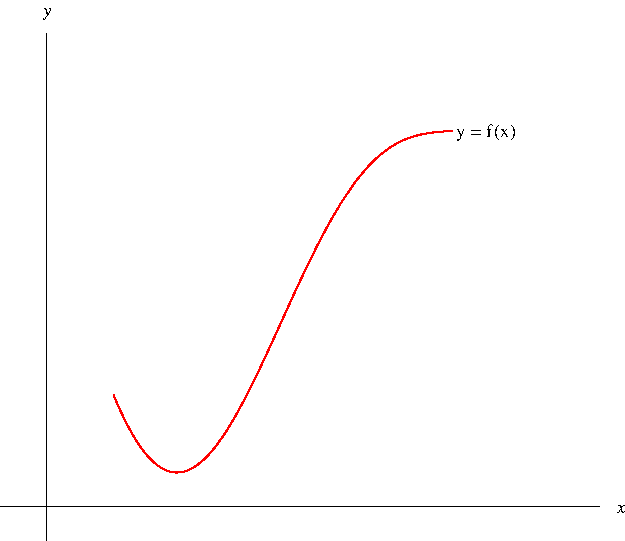
\includegraphics[height=5cm]{precalculus/pictures/01-01-function.pdf}
%}%
%\only<handout:1| 2>{%
%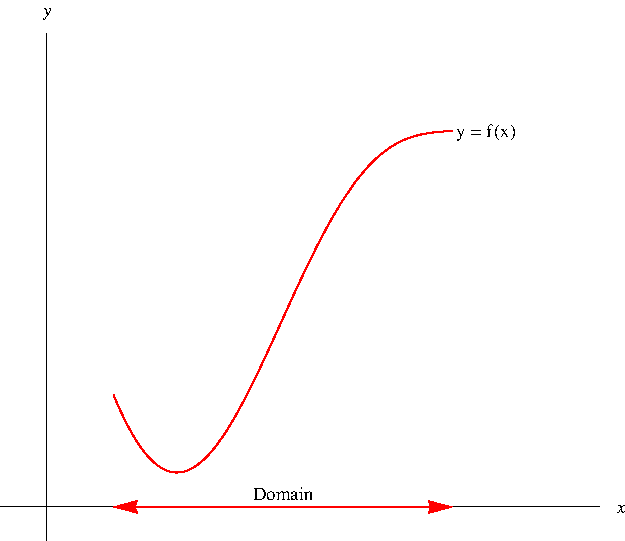
\includegraphics[height=5cm]{precalculus/pictures/01-01-domain.pdf}
%}%
%\only<handout:2| 3>{%
%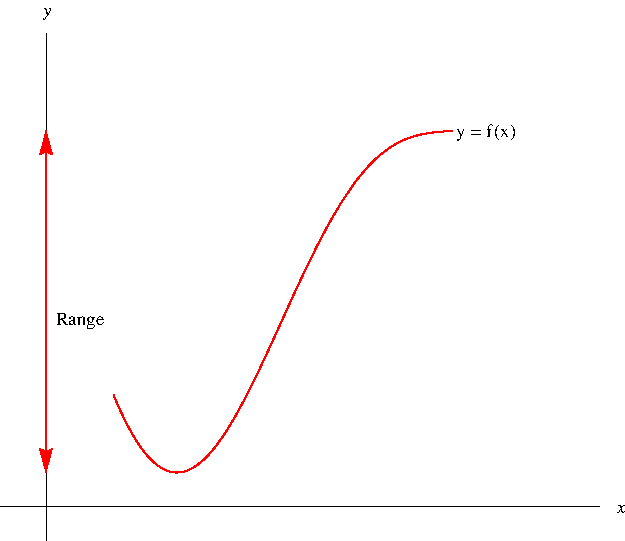
\includegraphics[height=5cm]{precalculus/pictures/01-01-range.pdf}
%}%
%\only<handout:3-| 4->{%
%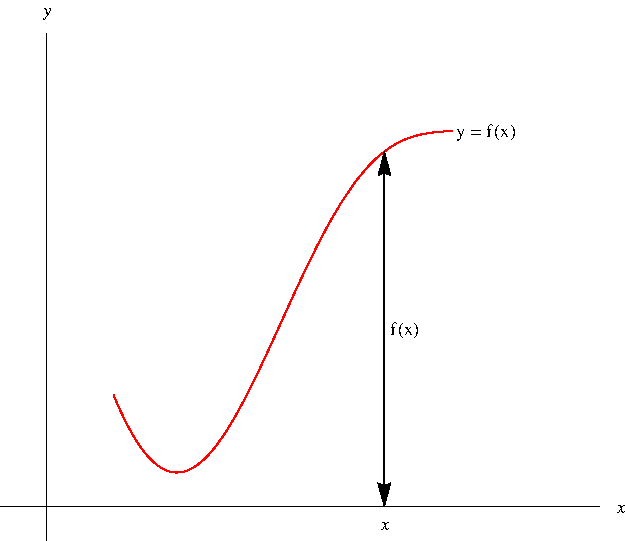
\includegraphics[height=5cm]{precalculus/pictures/01-01-fofx.pdf}
%}%

\begin{definition}[Function]
A function $f$ is a rule that assigns to each element $x$ in a set $D$ exactly one element, called $f(x)$, in a set $E$.
\end{definition}

\only<handout:3| 4>{
\begin{definition}[Range]
The set of all possible values taken by $f(x)$ as the element $x$ runs over elements of $D$ is called the range of $f$. 
\end{definition}
}

\only<handout:1| 2>{
\begin{definition}[Domain]
The set $D$ is called the domain. 
\end{definition}
}

\only<handout:2| 3>{
\begin{definition}[Co-domain]
The set $E$ is called the co-domain. 
\end{definition}
}

\only<handout:4| 5->{
\begin{definition}[Value of $f$ at $x$]
The number $f(x)$ is called the value of $f$ at $x$, and is read ``$f$ of $x$.''
\end{definition}
}

\uncover<4>{}
~\\~\\~\\~\\~\\~



\end{frame}
% end module function-def
\subsection{The Vertical Line Test}
% begin module vertical-line-test
\begin{frame}
\frametitle{The Vertical Line Test}
\begin{question}
Given a curve in the plane, is it the graph of a function or not?
\end{question}

\uncover<2->{The answer is as follows.
\begin{proposition}[The Vertical Line Test]
A curve in the plane is the graph of a function if and only if no vertical line intersects it more than once.
\end{proposition}
}

\begin{tabular}{ccc}
\psset{xunit=0.35cm, yunit=0.35cm}
\begin{pspicture}(-5, -5)(5,5) 
\psframe*[linecolor=white](-5,-5)(5,5) 
\psaxes[ticks=none, labels=none]{<->}(0,0)(-4.5,-4.5)(4.5,4.5)\tiny
%Function formula: sin{}(x) 
\psplot[linecolor=red, plotpoints=1000]{-5}{5}{x 57.29578 mul sin }
\end{pspicture}
%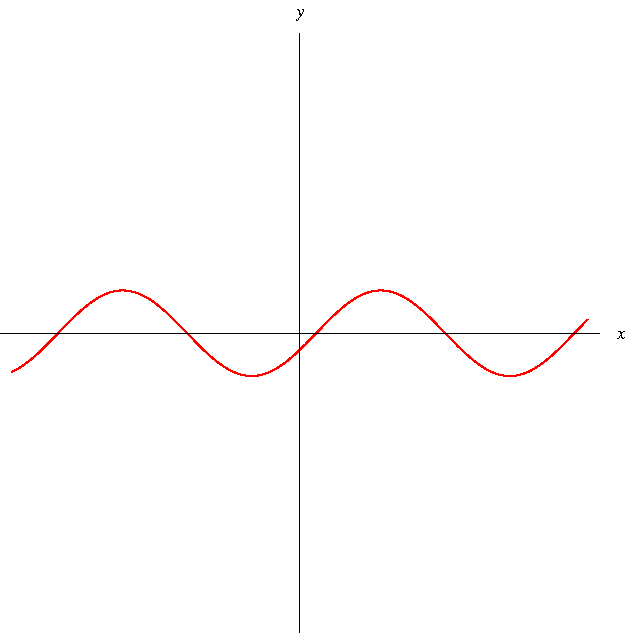
\includegraphics[height=3.8cm]{precalculus/pictures/01-02-vlt3.pdf} 
&%
\psset{xunit=0.35cm, yunit=0.35cm}
\begin{pspicture}(-5, -5)(5,5) \psframe*[linecolor=white](-5,-5)(5,5) 
\psaxes[ticks=none, labels=none]{<->}(0,0)(-4.5,-4.5)(4.5,4.5)\parametricplot[linecolor=red, plotpoints=1000]{0.05}{3}{t t 2.2 mul 57.29578 mul sin 1 add add t 57.29578 mul cos mul t t 2.2 mul 57.29578 mul sin 1 add add t 57.29578 mul sin mul}
\only<handout| 6->{%
\psline(1.7, -4.5)(1.7, 4.5)
}
\end{pspicture}
%\only<handout:0| -2>{%
%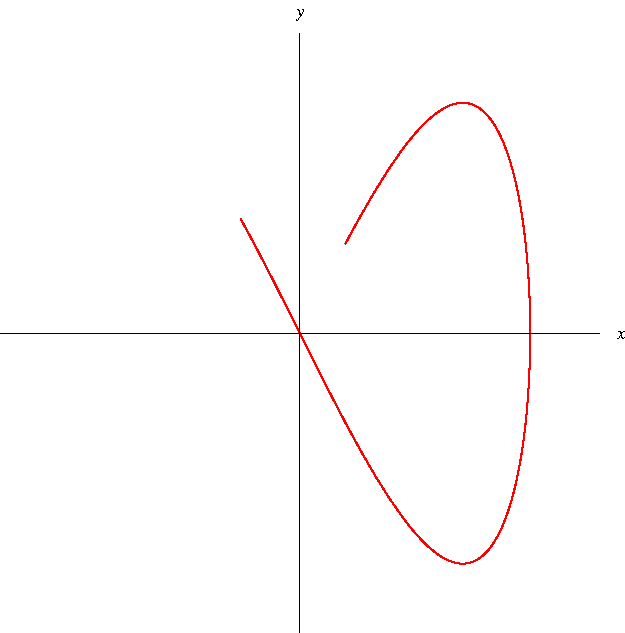
\includegraphics[height=3.8cm]{precalculus/pictures/01-02-vlt1a.pdf}%
%}%
%\only<handout| 3->{%
%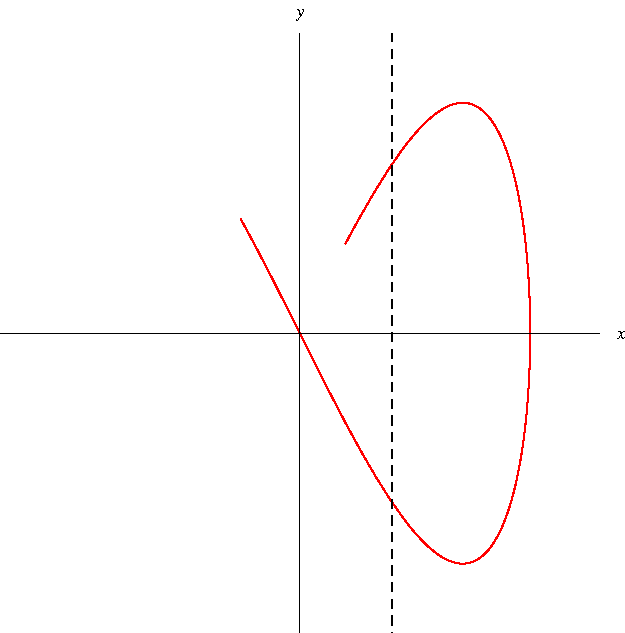
\includegraphics[height=3.8cm]{precalculus/pictures/01-02-vlt1b.pdf}%
%} 
&%
\psset{xunit=0.35cm, yunit=0.35cm}
\begin{pspicture}(-5, -5)(5,5) 
\psframe*[linecolor=white](-5,-5)(5,5) 
\psaxes[ticks=none, labels=none]{<->}(0,0)(-4.5,-4.5)(4.5,4.5)\tiny
%Function formula: 3/8+3/2 ((x)^{2})+1/4 (x)- ((x)^{3}) 
\psplot[linecolor=red, plotpoints=1000]{-0.5}{2}{x 3 exp -1 mul x 0.25 mul x 2 exp 1.5 mul 0.375 add add add } %Function formula: 1+1/2 (x) 
\psplot[linecolor=red, plotpoints=1000]{-4}{-0.5}{x 0.5 mul 1 add }
\end{pspicture} 
%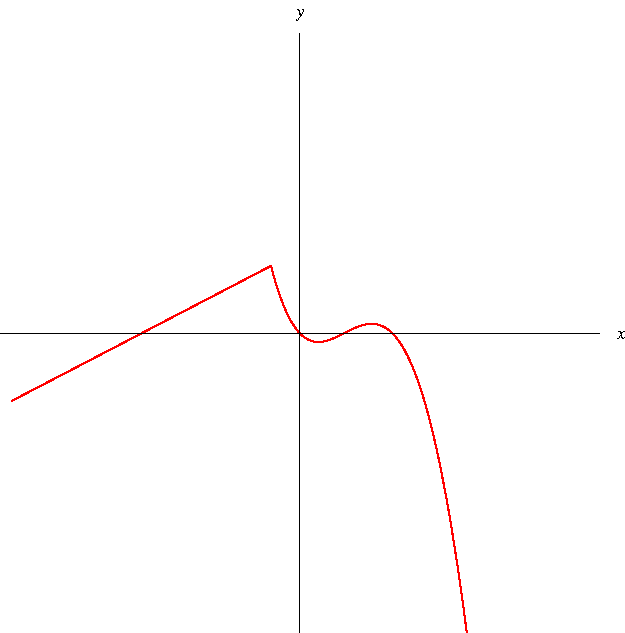
\includegraphics[height=3.8cm]{precalculus/pictures/01-02-vlt2.pdf} 
\\%
\fcAnswerUncoverNoH{1}{4}{Function} &
\fcAnswerUncoverNoH{1}{6}{Not a function}&
\fcAnswerUncoverNoH{1}{8}{Function}
\end{tabular}
\end{frame}
% end module vertical-line-test

\subsection{Piecewise Defined Functions}
% begin module function-piecewise
\begin{frame}
\frametitle{Piecewise Defined Functions}
\begin{definition}[Piecewise Defined Function]
A piecewise defined function is a function that is defined by different algebraic formulas on different subsets of its domain.
\end{definition}
\uncover<2->{
\begin{example}
\begin{columns}[t]
\column{.4\textwidth}
\ 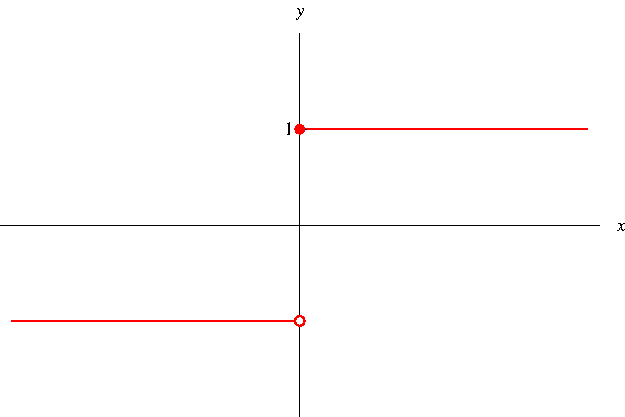
\includegraphics[height=3.5cm]{precalculus/pictures/01-01-piecewise.pdf}
\column{.5\textwidth}
\[
f(x) = \left\{ \begin{array}{rcc}
1 & \textrm{ if } & x \geq 0 \\
-1 & \textrm{ if } & x < 0 
\end{array}\right. 
\]

The filled red circle means $(0,1)$ is on the curve.  

The open circle means $(0, -1)$ is not on the curve.
\end{columns}
\end{example}
}
\end{frame}
% end module function-piecewise

% begin module absolute-value 
\begin{frame}
\begin{example}[Example 8, p. 18]
The absolute value $|a|$ of a number $a$ is defined to be
\[
|a| = \left\{ \begin{array}{ccccl}
\alert<handout:0| 2-3>{a} & \alert<handout:0| 3>{\textrm{if}} & \alert<handout:0| 3>{ a} & \alert<handout:0| 3>{\geq} & \alert<handout:0| 3>{0} \\
\alert<handout:0| 4-5>{-a} & \alert<handout:0| 5>{\textrm{if}} &  \alert<handout:0| 5>{a} & \alert<handout:0| 5>{<} & \alert<handout:0| 5>{0}. \end{array}\right.
\]

Sketch a graph of the function $f(x) = |x|$.

\begin{center}
\ \only<handout:0| 1>{%
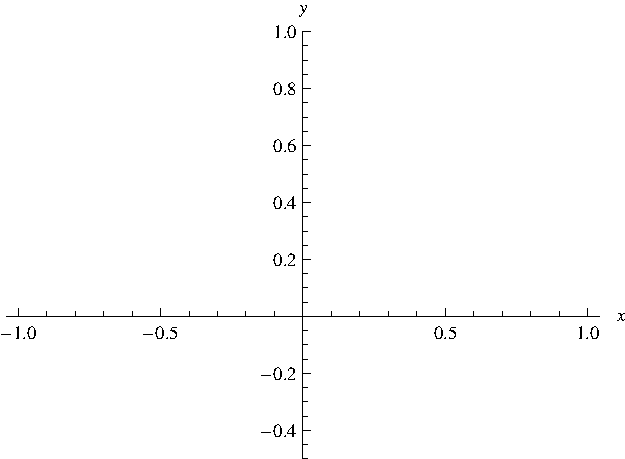
\includegraphics[height=4cm]{precalculus/pictures/01-01-ex-08a.pdf}%
}%
\only<handout:0| 2>{%
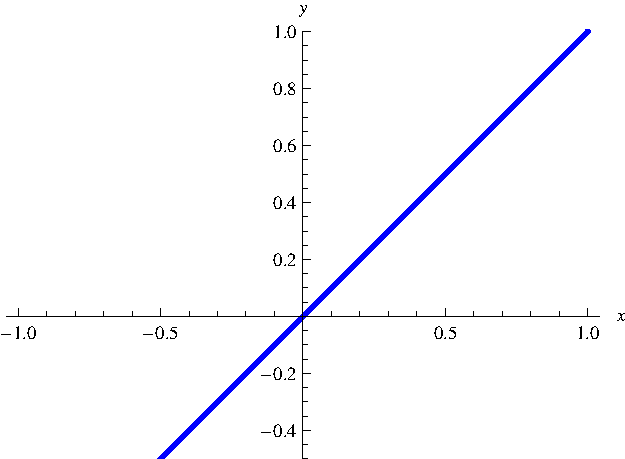
\includegraphics[height=4cm]{precalculus/pictures/01-01-ex-08b.pdf}%
}%
\only<handout:0| 3>{%
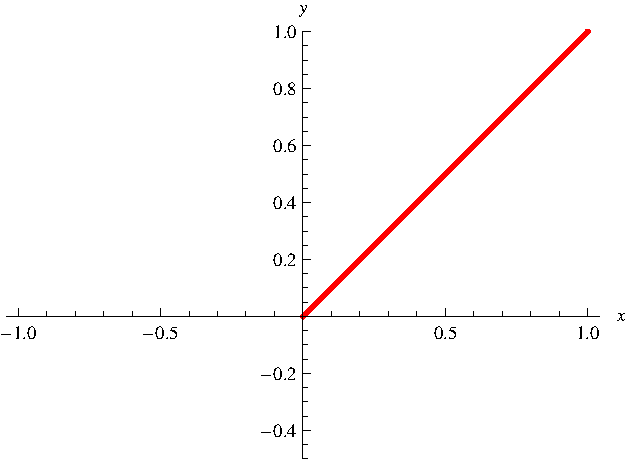
\includegraphics[height=4cm]{precalculus/pictures/01-01-ex-08c.pdf}%
}%
\only<handout:0| 4>{%
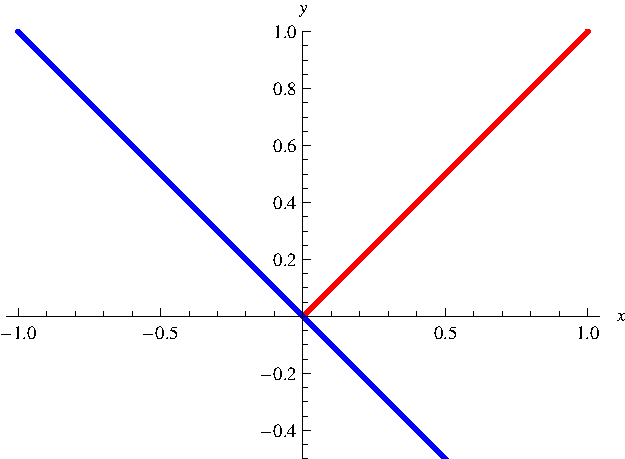
\includegraphics[height=4cm]{precalculus/pictures/01-01-ex-08d.pdf}%
}%
\only<handout:1-| 5>{%
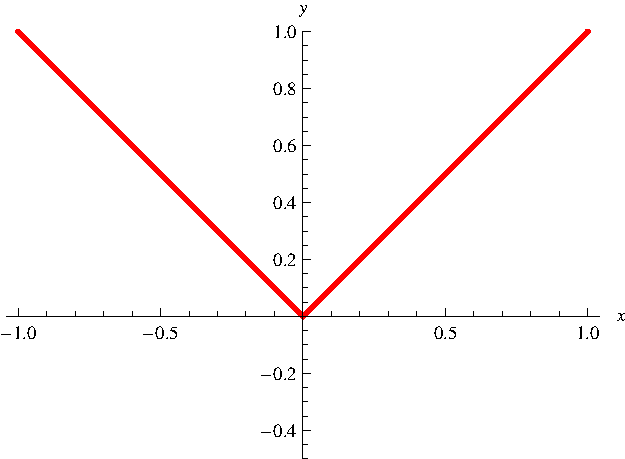
\includegraphics[height=4cm]{precalculus/pictures/01-01-ex-08e.pdf}%
}%
\end{center}
\end{example}
\end{frame}
% end module absolute-value 

% begin module piecewise-formula
\begin{frame}
\begin{example} %[Example 9, p. 18]
Find a formula for the function $f$ in the graph.

\psset{xunit=1.2cm, yunit=1.2cm}
\begin{pspicture}(-4, -0.5)(4,4) 
\tiny
\psframe*[linecolor=white](-5,-5)(5.2,5.2) 
\psaxes{<->}(0,0)(-0.5,-0.5)(5.2,2.2)
\psLabels{5.1}{2.2}
\psline[linecolor=red](0,0)(1,1)(2,0)(5,0)
\psHollowDot{5}{0}
\psFullDot{0}{0}
\only<4-5>{
\psline[linecolor=blue](-0.5, -0.5)(2,2)
}
\only<6-7>{
\psline[linecolor=blue](-0.2, 2.2)(2.5,-0.5)
}
\only<8-9>{
\psline[linecolor=blue](2, 0)(5,0)
}
\end{pspicture} 
%\ \only<1-3,10>{%
%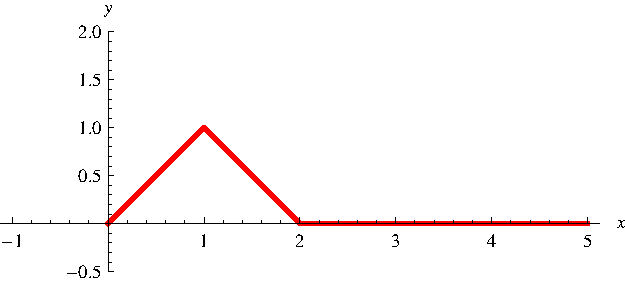
\includegraphics[height=4cm]{precalculus/pictures/01-01-ex-09a.pdf}%
%}%
%\only<handout:0| 4-5>{%
%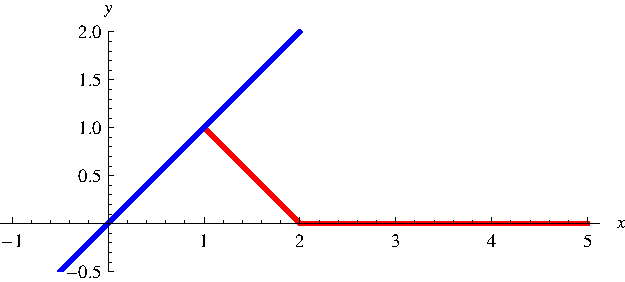
\includegraphics[height=4cm]{precalculus/pictures/01-01-ex-09b.pdf}%
%}%
%\only<handout:0| 6-7>{%
%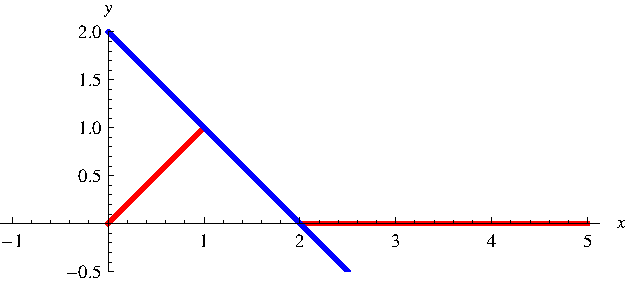
\includegraphics[height=4cm]{precalculus/pictures/01-01-ex-09c.pdf}%
%}%
%\only<handout:0| 8-9>{%
%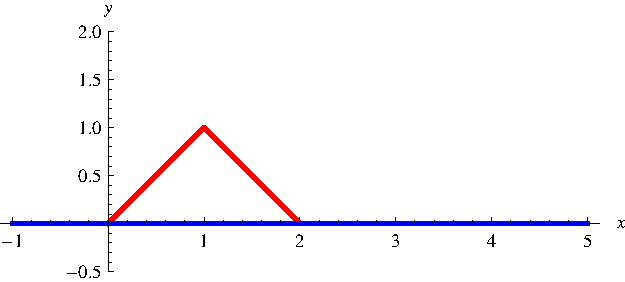
\includegraphics[height=4cm]{precalculus/pictures/01-01-ex-09d.pdf}%
%}%

\uncover<2->{
Different formulas on $[0, 1)$, $[1, 2)$, and $[2, 5)$. 
}

\uncover<3->{
\[
f(x) = \left\{ \begin{array}{ccccccl}
\uncover<5->{\alert<handout:0| 5>{x}} & \alert<handout:0| 4-5>{\textrm{if}} & \alert<handout:0| 4-5>{0} & \alert<handout:0| 4-5>{\leq} & \alert<handout:0| 4-5>{x} & \alert<handout:0| 4-5>{<} & \alert<handout:0| 4-5>{1} \\
\uncover<7->{\alert<handout:0| 7>{2 - x}} & \alert<handout:0| 6-7>{\textrm{if}} & \alert<handout:0| 6-7>{1} & \alert<handout:0| 6-7>{\leq} & \alert<handout:0| 6-7>{x} & \alert<handout:0| 6-7>{<} & \alert<handout:0| 6-7>{2} \\
\uncover<9->{\alert<handout:0| 9>{0}} & \alert<handout:0| 8-9>{\textrm{if}} & \alert<handout:0| 8-9>{2} & \alert<handout:0| 8-9>{\leq} & \alert<handout:0| 8-9>{x} & \alert<handout:0| 8-9>{<} & \alert<handout:0| 8-9>{5} \end{array}\right.
\]
}
\end{example}
\end{frame}
% end module piecewise-formula

% WARNING: The next two modules have the wrong pictures.
% begin module piecewise-ex1
\begin{frame}
\begin{example}
Sketch the function $f(x)  = |2x-3|$.
\begin{columns}
\column{.4\textwidth}
\psset{xunit=1.6cm, yunit=1.6cm}
\begin{pspicture}(-0.5, -0.5)(2.8,2.8)
\tiny
\psframe*[linecolor=white](-0.5,-0.5)(2.8,2.8)
\psaxes{<->}(0,0)(-0.5,-0.5)(2.75,2.5)
\fcLabels{2.75}{2.5}
\uncover<6->{
\psline[linecolor=red](1.5, 0)(2.75,2.5)
}
\uncover<7->{
\psline[linecolor=red](0.25,2.5)(1.5, 0)
}
\end{pspicture}
%\only<-5| handout:0>{%
%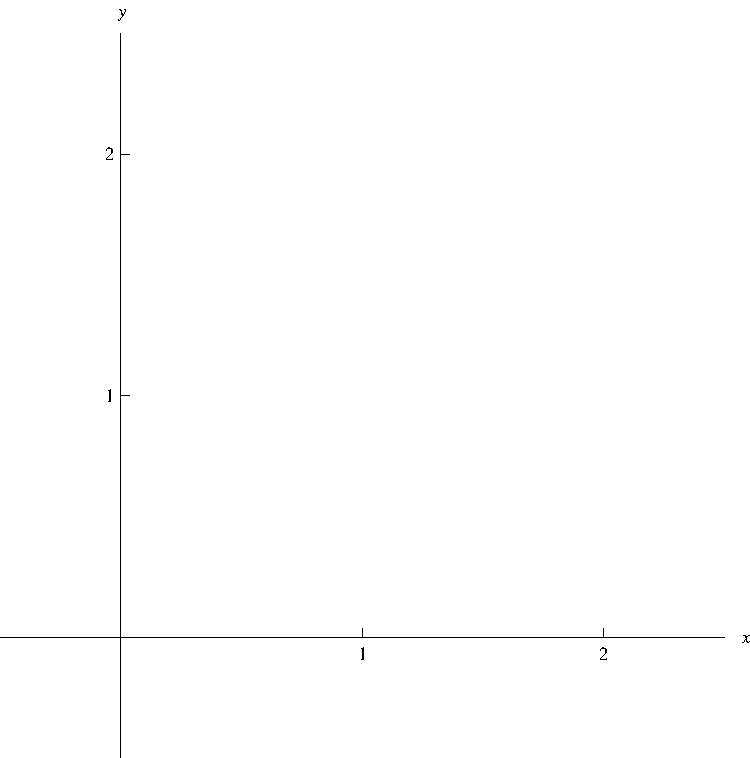
\includegraphics[width=4.5cm]{precalculus/pictures/piecewise-ex1-1.pdf}%
%}%
%\only<6| handout:0>{%
%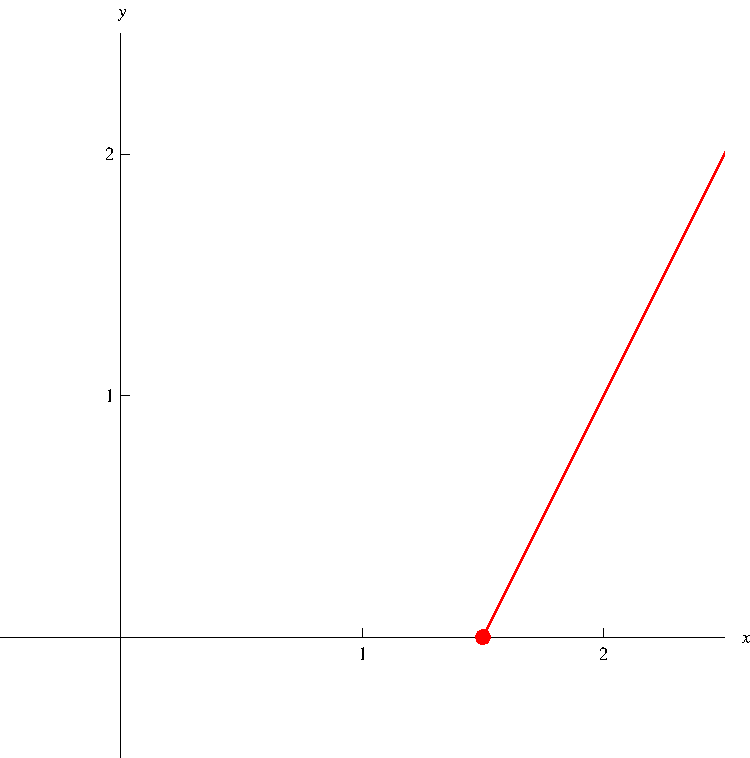
\includegraphics[width=4.5cm]{precalculus/pictures/piecewise-ex1-2.pdf}%
%}%
%\only<7-| handout:1>{%
%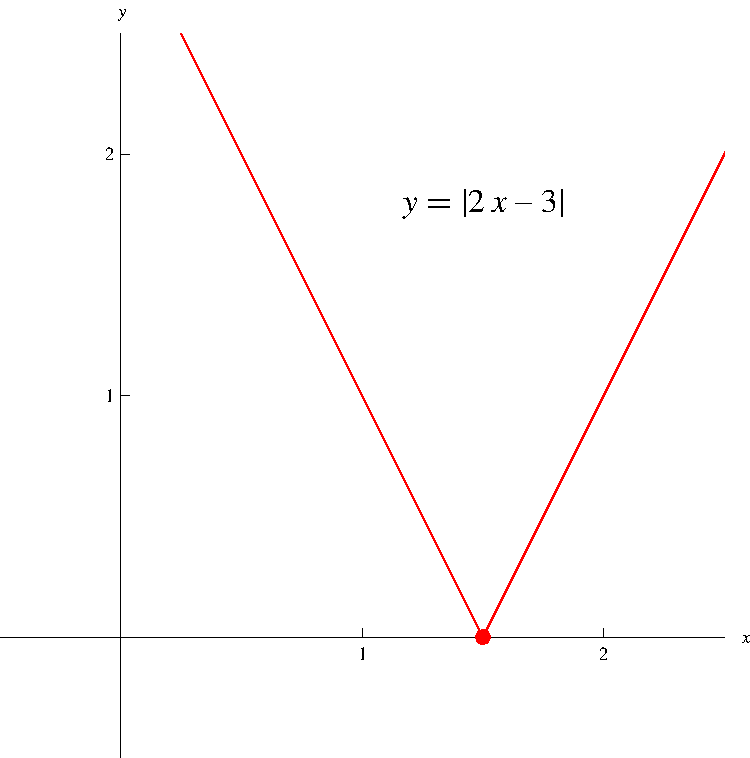
\includegraphics[width=4.5cm]{precalculus/pictures/piecewise-ex1-3.pdf}%
%}%
\column{.55\textwidth}
\abovedisplayskip=0pt
\belowdisplayskip=-15pt
\abovedisplayshortskip=0pt
\belowdisplayshortskip=0pt
\begin{align*}
\uncover<2->{%
|\alert<handout:0| 3>{x}| %
}%
& \uncover<2->{%
 = \begin{cases}
\alert<handout:0| 3>{x} & \text{if $\alert<handout:0| 3>{x} \geq 0$}\\
-\alert<handout:0| 3>{x} & \text{if $\alert<handout:0| 3>{x} < 0$}.\\
\end{cases}
}\\%
\uncover<3->{%
|\alert<handout:0| 3>{2x-3}| %
}%
& \uncover<3->{%
 = \begin{cases}
\alert<handout:0| 3>{2x-3} & \text{if $\alert<handout:0| 3>{2x-3} \geq 0$}\\
-(\alert<handout:0| 3>{2x-3}) & \text{if $\alert<handout:0| 3>{2x-3} < 0$}\\
\end{cases}
}\\%
& \uncover<4->{%
 = \begin{cases}
2x-3 & \text{if $2x \geq 3$}\\
-2x+3 & \text{if $2x < 3$}\\
\end{cases}
}\\%
& \uncover<5->{%
 = \begin{cases}
\alert<handout:0| 6>{2x-3} & \alert<handout:0| 6>{\text{if $x \geq 3/2$}}\\
\alert<handout:0| 7>{-2x+3} & \alert<handout:0| 7>{\text{if $x < 3/2$}}.\\
\end{cases}
}%
\end{align*}
\end{columns}
\end{example}
\end{frame}
% end module piecewise-ex1

% begin module piecewise-ex2
\begin{frame}
\begin{example}
Sketch the function $\displaystyle f(x)  = \frac{|4x+2|}{2x+1}$.
\begin{columns}
\column{.4\textwidth}
\psset{xunit=1cm, yunit=1cm}
\begin{pspicture}(-4, -0.5)(4,4) 
\tiny
\psframe*[linecolor=white](-5,-5)(5.2,5.2) 
\psaxes{<->}(0,0)(-3.2,-3.2)(2.2,3.2)
\psLabels{2.2}{3.2}
\uncover<9->{
\psline[linecolor=red](-0.5, 2)(2.2,2)
\psHollowDot{-0.5}{2}
}
\uncover<10->{
\psline[linecolor=red](-0.5,-2)(-3, -2)
\psHollowDot{-0.5}{-2}
}
\end{pspicture} 
%\only<-8| handout:0>{%
%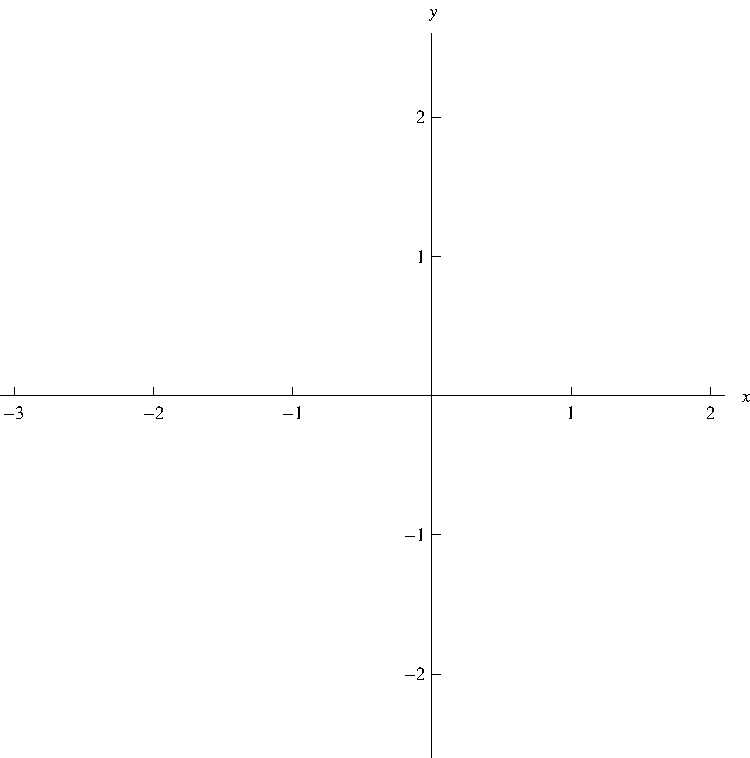
\includegraphics[width=4.5cm]{precalculus/pictures/piecewise-ex2-1.pdf}%
%}%
%\only<9| handout:0>{%
%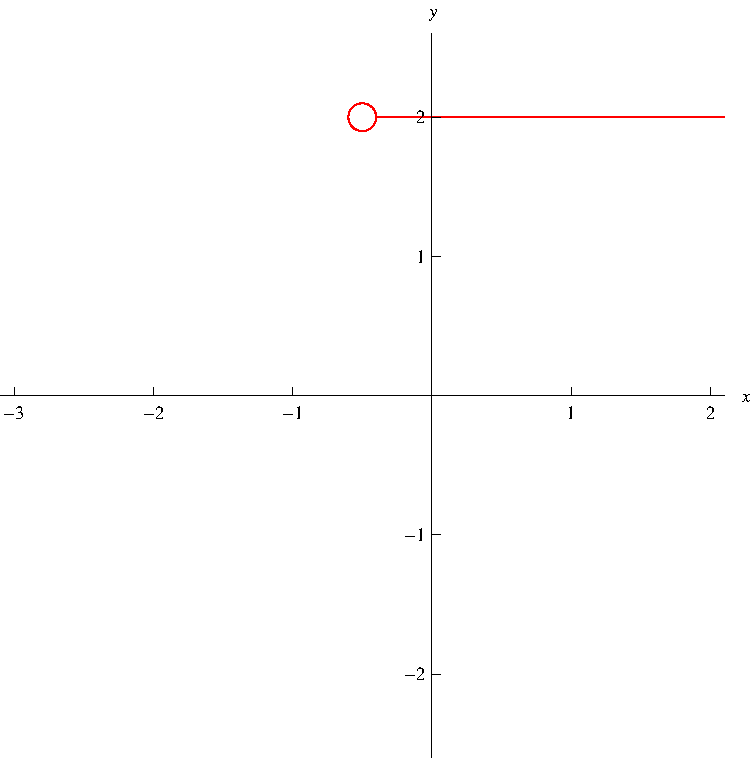
\includegraphics[width=4.5cm]{precalculus/pictures/piecewise-ex2-2.pdf}%
%}%
%\only<10-| handout:1>{%
%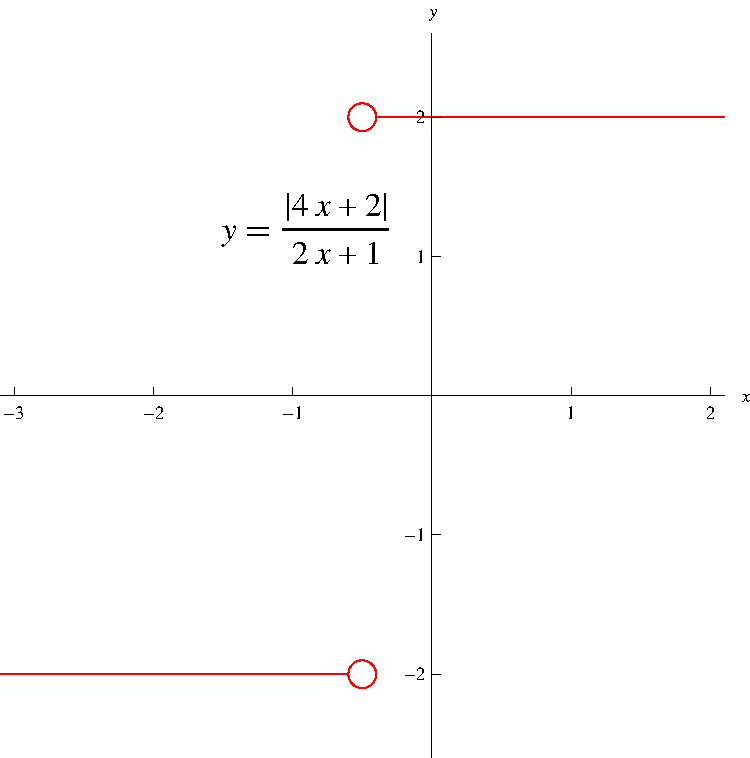
\includegraphics[width=4.5cm]{precalculus/pictures/piecewise-ex2-3.pdf}%
%}%
\column{.55\textwidth}
\abovedisplayskip=0pt
\belowdisplayskip=-15pt
\abovedisplayshortskip=0pt
\belowdisplayshortskip=0pt
\begin{align*}
\uncover<2->{%
|\alert<handout:0| 3>{x}| %
}%
& \uncover<2->{%
 = \begin{cases}
\alert<handout:0| 3>{x} & \text{if $\alert<handout:0| 3>{x} \geq 0$}\\
-\alert<handout:0| 3>{x} & \text{if $\alert<handout:0| 3>{x} < 0$}.\\
\end{cases}
}\\%
\uncover<3->{%
\frac{|\alert<handout:0| 3>{4x+2}|}{2x+1} %
}%
& \uncover<3->{%
 = \begin{cases}
\frac{\alert<handout:0| 3-5>{4x+2}}{2x+1} & \text{if $\alert<handout:0| 3>{4x+2} > 0$}\\
\frac{\alert<handout:0| 6-7>{-(\alert<handout:0| 3>{4x+2})}}{2x+1} & \text{if $\alert<handout:0| 3>{4x+2} < 0$}\\
\end{cases}
}\\%
& \uncover<4->{%
 = \begin{cases}
\frac{\uncover<5->{\alert<handout:0| 5>{2(2x+1)}}}{2x+1} & \text{if $4x > -2$}\\
\frac{\uncover<7->{\alert<handout:0| 7>{-2(2x+1)}}}{2x+1} & \text{if $4x < -2$}\\
\end{cases}
}\\%
& \uncover<8->{%
 = \begin{cases}
\alert<handout:0| 9>{2} & \alert<handout:0| 9>{\text{if $x > -1/2$}}\\
\alert<handout:0| 10>{-2} & \alert<handout:0| 10>{\text{if $x < -1/2$}}.\\
\end{cases}
}%
\end{align*}
\end{columns}
\end{example}
\end{frame}
% end module piecewise-ex2

\subsection{Symmetry}
% begin module even-and-odd
\begin{frame}
\frametitle{Symmetry}
\begin{definition}[Even and Odd Functions]
A function $f$ is called even if $f(-x) = f(x)$ for all $x$ in its domain.  A function $f$ is called odd if $f(-x) = -f(x)$ for all $x$ in its domain.
\end{definition}
\uncover<2->{
\begin{example}[$x^2$ is Even, $x^3$ is Odd]
The function $f(x) = x^2$ is even:
\uncover<3->{
\[
f(-x) = (-x)^2 = x^2 = f(x) .
\]
}
The function $g(x) = x^3$ is odd:
\uncover<4->{
\[
g(-x) = (-x)^3 = -x^3 = -g(x) .
\]
}
\end{example}
}
\end{frame}

\begin{frame}
\begin{definition}[Even and Odd Functions]
A function $f$ is called even if $f(-x) = f(x)$ for all $x$ in its domain.  A function $f$ is called odd if $f(-x) = -f(x)$ for all $x$ in its domain.
\end{definition}
\begin{example}[Example 11, p. 19]
Determine whether each of the following functions is even, odd, or neither even nor odd.

\begin{columns}[t]
\column{.33\textwidth}
\[
f(x) = x^5 + x
\]
\[
\begin{array}{r@{ \ }c@{ \ }l}
\uncover<2->{f(-x)} & \uncover<2->{=} & \uncover<3->{(-x)^5 + (-x)} \\
& \uncover<4->{=} & \uncover<4->{-x^5 - x} \\
& \uncover<5->{=} & \uncover<5->{-(x^5 + x)} \\
& \uncover<6->{=} & \uncover<6->{-f(x)} 
\end{array}
\]
\uncover<7->{
Therefore $f$ is odd.
}
\column{.33\textwidth}
\[
g(x) = 1 - x^4
\]
\[
\begin{array}{r@{ \ }c@{ \ }l}
\uncover<2->{g(-x)} & \uncover<2->{=} & \uncover<8->{1 - (-x)^4} \\
& \uncover<9->{=} & \uncover<9->{1 - x^4} \\
& \uncover<10->{=} & \uncover<10->{g(x)} 
\end{array}
\]
\uncover<11->{
Therefore $g$ is even.
}
\column{.33\textwidth}
\[
h(x) = 2x - 1
\]
\[
\begin{array}{r@{ \ }c@{ \ }l}
\uncover<2->{h(-x)} & \uncover<2->{=} & \uncover<12->{2(-x) - 1} \\
& \uncover<13->{=} & \uncover<13->{-2x - 1} \\
& \uncover<14->{\neq} & \uncover<14->{h(x), -h(x)}
\end{array}
\]
\uncover<15->{
Therefore $h$ is neither even nor odd.
}
\end{columns}
\end{example}
\end{frame}
% end module even-and-odd

\subsection{Increasing and Decreasing Functions}
% begin module increasing-decreasing
\begin{frame}
\frametitle{Increasing and Decreasing Functions}
\begin{definition}[Increasing and Decreasing Functions]
A function $f$ is called increasing on an interval $I$ if $f(x_1) < f(x_2)$ whenever $x_1 < x_2$  in $I$.  

It is called decreasing on the interval $I$ if $f(x_1) > f(x_2)$ whenever $x_1 < x_2$ in $I$.
\end{definition}
\uncover<2->{
\begin{example}[Increasing and Decreasing]
\begin{columns}[t]
\column{.6\textwidth}

\psset{xunit=3.4cm, yunit=3.4cm}
\begin{pspicture}(-1.1, -0.4)(1.15,0.7) 
\psframe*[linecolor=white](-1.1,-0.4)(1.15,0.7) 
\tiny
\psaxes[Dx=0.25, Dy=0.25]{<->}(0,0)(-1.1,-0.3)(1.1,0.6)
\psLabels{1.1}{0.6}
%Function formula: 7/40+13/10 ((x)^{3})-39/40 (x) 
\psplot[linecolor=red, plotpoints=1000]{-1}{1}{x -0.975 mul x 3 exp 1.3 mul 0.175 add add }
\uncover<3>{
\psplot[linecolor=blue, plotpoints=1000]{-1}{-0.5}{x -0.975 mul x 3 exp 1.3 mul 0.175 add add }
}
\uncover<4>{
\psplot[linecolor=blue, plotpoints=1000]{-0.5}{0.5}{x -0.975 mul x 3 exp 1.3 mul 0.175 add add }
}
\uncover<5>{
\psplot[linecolor=blue, plotpoints=1000]{0.5}{1}{x -0.975 mul x 3 exp 1.3 mul 0.175 add add }
}
\end{pspicture} 
%\ \only<-2>{%
%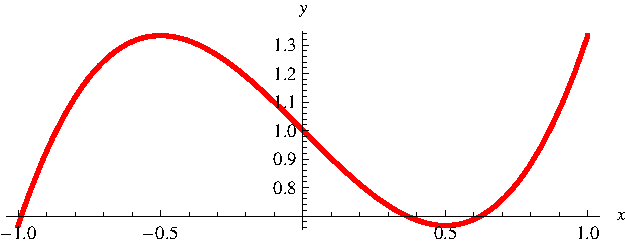
\includegraphics[height=2.8cm]{precalculus/pictures/01-01-inc-dec-a.pdf}%
%}%
%\only<handout:0| 3>{%
%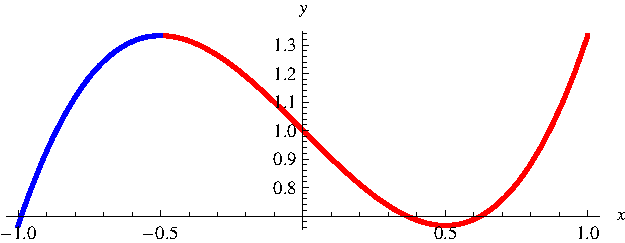
\includegraphics[height=2.8cm]{precalculus/pictures/01-01-inc-dec-b.pdf}%
%}%
%\only<handout:0| 4>{%
%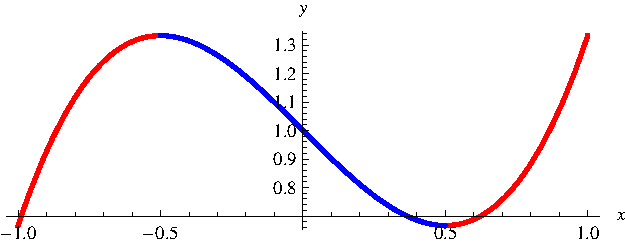
\includegraphics[height=2.8cm]{precalculus/pictures/01-01-inc-dec-c.pdf}%
%}%
%\only<handout:0| 5->{%
%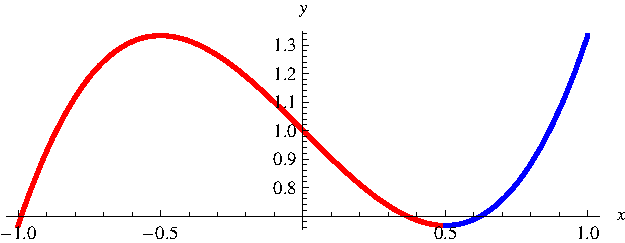
\includegraphics[height=2.8cm]{precalculus/pictures/01-01-inc-dec-d.pdf}%
%}%
\column{.4\textwidth}
\begin{itemize}
\item<3-| alert@3> \only<3>{\color{blue}} $f$ is increasing on $[-1, -\frac{1}{2}]$.
\item<4-| alert@4> \only<4>{\color{blue}} $f$ is decreasing on $[-\frac{1}{2}, \frac{1}{2}]$.
\item<5-| alert@5> \only<5>{\color{blue}} $f$ is increasing on $[\frac{1}{2}, 1]$.
\end{itemize}
\end{columns}
\end{example}
}
\end{frame}
% end module increasing-decreasing

\subsection{A Note on Domains of Functions}
% begin module domains
\begin{frame}
\frametitle{A Note on Domains of Functions}
If the domain of a function isn't specified, it is assumed to be all numbers $x$ for which the formula $f(x)$ is defined.  There are some restrictions to consider:
\begin{itemize}
\item<2->  Can't divide by $0$.
\item<3->  Can't take the even root of a negative number ($\sqrt{-1} , \sqrt[4]{-2053}, \sqrt[6]{-15} \ldots$ not allowed).
\item<4->  Can't take $\log x$ if $x \leq 0$.  
\end{itemize}
\end{frame}

\begin{frame}
\begin{example}[Two Functions and Their Domains]
Find the domains of the following two functions:
\begin{columns}
\column{.5\textwidth}
\[
f(x) = \alert<handout:0| 5>{\sqrt[4]{x-2}} + \sqrt[3]{6-x}
\]
\begin{itemize}
\item<2->  Any risk of dividing by $0$?  \uncover<3->{No.}
\item<4->  Any risk of taking the even root of a negative number? \uncover<5->{\alert<handout:0| 5>{Yes.}}
\item<6->  $x - 2$ can't be negative.
\end{itemize}
\begin{eqnarray*}
\uncover<7->{x - 2} & \uncover<7->{\geq} & \uncover<7->{0}\\
\uncover<8->{x} & \uncover<8->{\geq} & \uncover<8->{2}
\end{eqnarray*}
\uncover<9->{Domain is all real numbers bigger than or equal to $2$; that is, $[2,\infty )$.
}%
\column{.5\textwidth}
\[
g(x) = \frac{x^2 - 9}{\alert<handout:0| 11>{x^2 - x - 6}}
\]
\begin{itemize}
\item<10->  Any risk of dividing by $0$?  \uncover<11->{\alert<handout:0| 11>{Yes.}}
\item<12->  Any risk of taking the even root of a negative number? \uncover<13->{No.}
\item<14->  $x^2 - x - 6$ can't be $0$.
\end{itemize}
\abovedisplayskip=0pt
\belowdisplayskip=0pt
\abovedisplayshortskip=0pt
\belowdisplayshortskip=0pt
\begin{eqnarray*}
\uncover<15->{x^2 - x - 6} & \uncover<15->{\neq} & \uncover<15->{0}\\
\uncover<16->{(x - 3)(x + 2)} & \uncover<16->{\neq} & \uncover<16->{0}\\
\uncover<17->{x} & \uncover<17->{\neq} & \uncover<17->{3 \textrm{ or } -2}\\
\end{eqnarray*}
\uncover<18->{Domain is all real numbers except $3$ and $-2$; that is, \\ $(-\infty , -2)$ $\cup (-2,3)$ $\cup (3,\infty )$.
}%
\end{columns}
\end{example}
\end{frame}
% end module domains

\section{(1.2) A Catalog of Essential Functions}
\subsection{Linear Functions}
% begin module linear-functions
\begin{frame}
\frametitle{Linear Functions}
\begin{definition}[Linear Function]
A linear function is a function the graph of which is a line.  We can write any linear function in slope-intercept form:
\[
f(x) = mx + b.
\]
$m$ is called the slope, and $b$ is called the $y$-intercept.
\end{definition}
\end{frame}

\begin{frame}
\begin{columns}[c]
\column{.5\textwidth}

\psset{xunit=0.7cm, yunit=0.7cm}
\begin{pspicture}(-5, -5)(5,5) 
\psframe*[linecolor=white](-5,-5)(5,5) 
\tiny
\psaxes[ticks=none, labels=none]{<->}(0,0)(-2.5,-2.5)(5,2.5)
\psLabels{5}{2.5}
\psLabelXOne
\uncover<2>{
\psline[linecolor=red](-2.5, -1.5)(1.5, 2.5)
}
\uncover<3->{
\psline[linecolor=blue](-2.5, -1.5)(1.5, 2.5)
}
\uncover<2->{
\rput[l](1.5, 2){$y=x+1$}
}
\uncover<5->{
\psFullDot{0}{1}
\rput[r](-0.1, 1){\alert<5>{$(0,1)$}}
}

\uncover<3>{
\psline[linecolor=red](-2.5, 1.25)(5, -2.5)
}
\uncover<4->{
\psline[linecolor=blue](-2.5, 1.25)(5, -2.5)
}
\uncover<3->{
\rput[r](3.3, -2){$y=-0.5x$}
}
\uncover<6->{
\psFullDot{0}{0}
\rput[lb](0.1, 0.1){\alert<6>{$(0,0)$}}
}

\uncover<4>{
\psline[linecolor=red](-2.5,-1)(5, -1)
}
\uncover<5->{
\psline[linecolor=blue](-2.5, -1)(5, -1)
}
\uncover<4->{
\rput[t](4, -1.1){$y=-1$}
}
\uncover<7->{
\psFullDot{0}{-1}
\rput[lt](0.1, -1.1){\alert<7>{$(0,-1)$}}
}
\end{pspicture} 
%\ \only<handout:0| -2>{%
%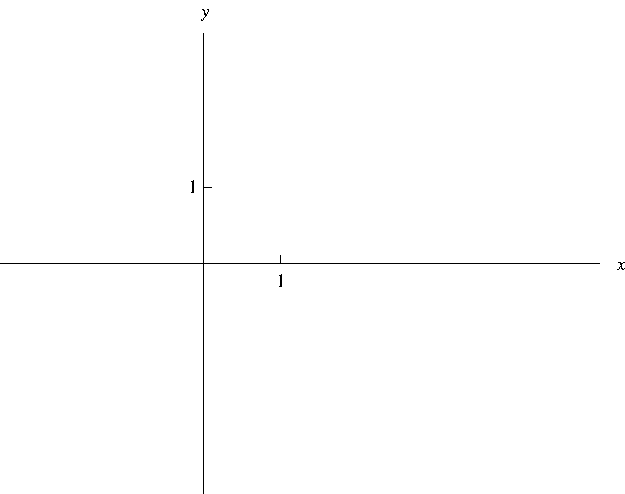
\includegraphics[height=4.5cm]{precalculus/pictures/01-02-linesa.pdf}%
%}%
%\only<handout:0| 3>{%
%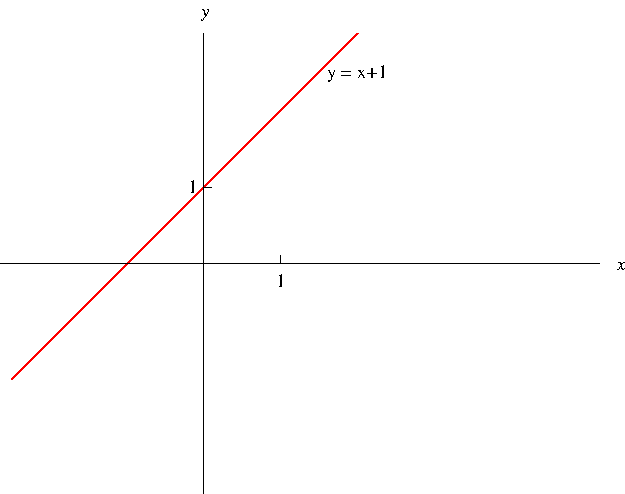
\includegraphics[height=4.5cm]{precalculus/pictures/01-02-linesb.pdf}%
%}%
%\only<handout:0| 4>{%
%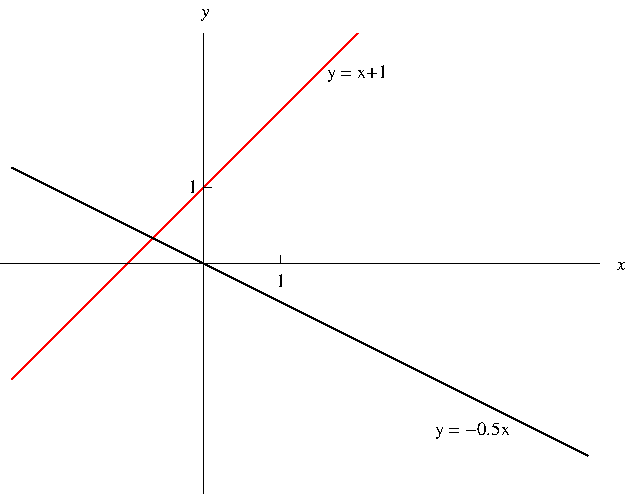
\includegraphics[height=4.5cm]{precalculus/pictures/01-02-linesc.pdf}%
%}%
%\only<handout:0| 5>{%
%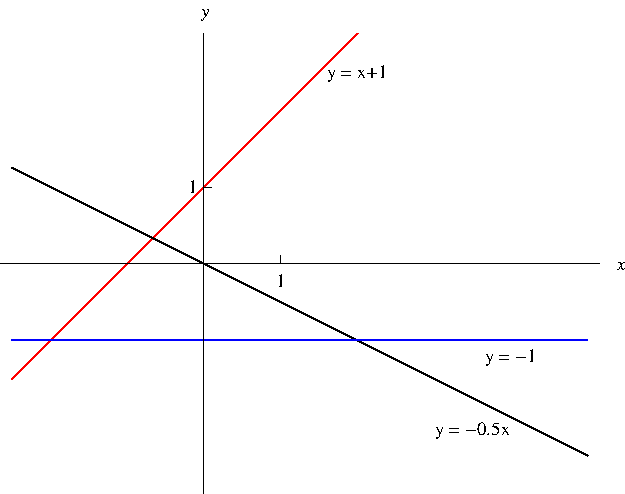
\includegraphics[height=4.5cm]{precalculus/pictures/01-02-linesd.pdf}%
%}%
%\only<handout:0| 6>{%
%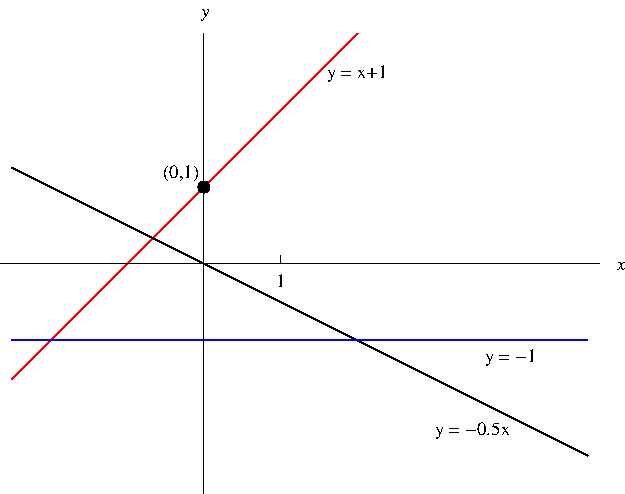
\includegraphics[height=4.5cm]{precalculus/pictures/01-02-linese.pdf}%
%}%
%\only<handout:0| 7>{%
%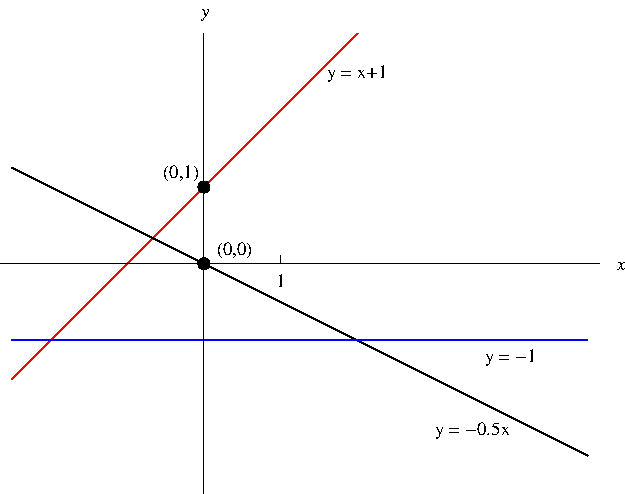
\includegraphics[height=4.5cm]{precalculus/pictures/01-02-linesf.pdf}%
%}%
%\only<8>{%
%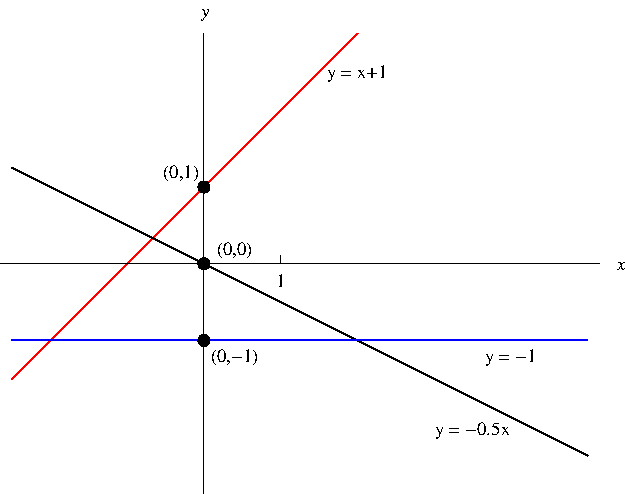
\includegraphics[height=4.5cm]{precalculus/pictures/01-02-linesg.pdf}%
%}%
\column[t]{.55\textwidth}
\begin{tabular}{|c|c|c|}
\hline
$f(x)$ & Direction & $y$-intercept \\
\hline
\uncover<1->{\alert<handout:0| 2>{$x + \alert<handout:0| 5>{1}$}} & 
\uncover<2->{\alert<handout:0| 2>{$\nearrow$}} & 
\uncover<5->{\alert<handout:0| 5>{1}} \\
\uncover<1->{\alert<handout:0| 3>{$-0.5x \uncover<6>{\alert<handout:0| 6>{+ 0}}$}} & 
\uncover<3->{\alert<handout:0| 3>{$\searrow$}} & 
\uncover<6->{\alert<handout:0| 6>{0}} \\
\uncover<1->{\alert<handout:0| 4,7>{$-1$}} & 
\uncover<4->{\alert<handout:0| 4>{$\rightarrow$}} & 
\uncover<7->{\alert<handout:0| 7>{-1}} \\
\hline
\end{tabular}
\end{columns}

\begin{itemize}
\item<2->  $m > 0$ means the graph of $f$ points up ($\nearrow$).
\item<3->  $m < 0$ means the graph of $f$ points down ($\searrow$).
\item<4->  $m = 0$ means the graph of $f$ is horizontal ($\rightarrow$).
\item<5->  $b$ tells us the height of the point where the graph hits the $y$-axis.
\end{itemize}
\end{frame}
% end module linear-functions

\subsection{Polynomials}
% begin module polynomials
\begin{frame}
\frametitle{Polynomials}
\begin{definition}[Polynomial Function]
A polynomial function is a function $f$ of the form
\[
f(x) = a_0 + a_1x + a_2x^2 + \cdots + a_{n - 1}x^{n-1} + a_nx^n ,
\]
where $n$ is a non-negative integer and $a_0, \ldots , a_n$ are real numbers, called the coefficients.

If the leading coefficient $a_n \neq 0$, then we say the degree of $f$ is $n$.
\end{definition}
\uncover<2->{
\[
\begin{array}{|c|c|c|c|c|c|}
\hline
f(x) &%
\alert<handout:0| 3-4,13-14,23-26,35-36>{\text{Polynomial?}} &%
\alert<handout:0| 5-6,15-16,27-28>{\text{Degree}} &%
\alert<handout:0| 7-8,17-18,29-30>{a_0} &%
\alert<handout:0| 9-10,19-20,31,32>{a_1} &%
\alert<handout:0| 11-12,21-22,33-34>{a_2} \\
\hline
\alert<handout:0| 3-12>{x^4-x+1} &%
\uncover<4->{\alert<handout:0| 4>{\text{Yes}}}&%
\uncover<6->{\alert<handout:0| 6>{4}}&%
\uncover<8->{\alert<handout:0| 8>{1}}&%
\uncover<10->{\alert<handout:0| 10>{-1}}&%
\uncover<12->{\alert<handout:0| 12>{0}}\\%
\alert<handout:0| 13-22>{6} &%
\uncover<14->{\alert<handout:0| 14>{\text{Yes}}}&%
\uncover<16->{\alert<handout:0| 16>{0}}&%
\uncover<18->{\alert<handout:0| 18>{6}}&%
\uncover<20->{\alert<handout:0| 20>{0}}&%
\uncover<22->{\alert<handout:0| 22>{0}}\\%
\alert<handout:0| 23>{3x^2 - \frac{1}{2}x + \alert<handout:0| 24>{\sqrt{x}}} &%
\uncover<24->{\alert<handout:0| 24>{\text{No}}}&%
&%
&%
&\\
\alert<handout:0| 25-34>{3x^2 - \frac{1}{2}x + \sqrt{2}} &%
\uncover<26->{\alert<handout:0| 26>{\text{Yes}}}&%
\uncover<28->{\alert<handout:0| 28>{2}}&%
\uncover<30->{\alert<handout:0| 30>{\sqrt{2}}}&%
\uncover<32->{\alert<handout:0| 32>{-\frac{1}{2}}}&%
\uncover<34->{\alert<handout:0| 34>{3}}\\%
\alert<handout:0| 35>{3x^2 - \frac{1}{2\alert<handout:0| 36>{x}} + \sqrt{2}} &%
\uncover<36->{\alert<handout:0| 36>{\text{No}}}&%
&%
&%
&\\
\hline
\end{array}
\]
}
\end{frame}


\begin{frame}
\begin{itemize}
\item<1->  Linear functions are polynomials.
\item<2->  So are quadratic functions.  Their graphs are parabolas.
\item<3->  And there are many more.
\end{itemize}
\only<handout:1| 1>{%
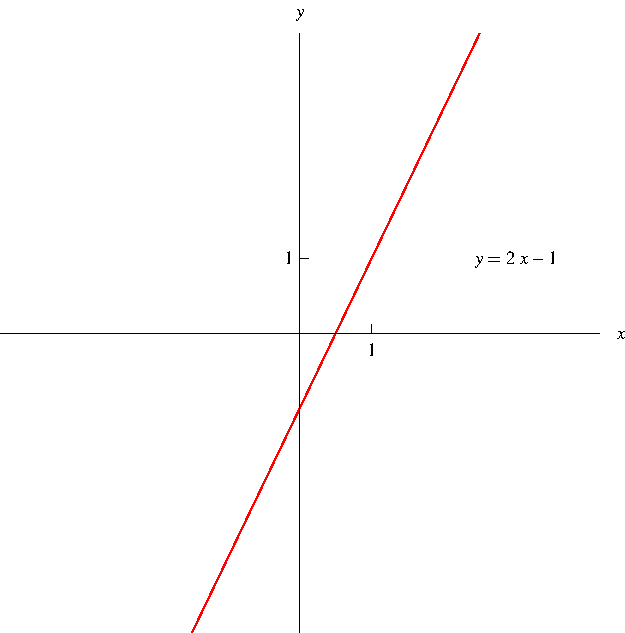
\includegraphics[height=6cm]{precalculus/pictures/01-02-line.pdf}%

Linear
}%
\only<handout:2| 2>{%
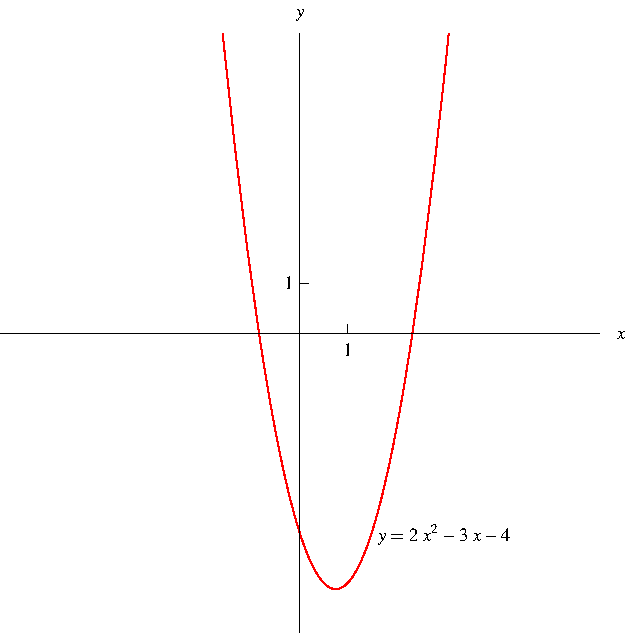
\includegraphics[height=6cm]{precalculus/pictures/01-02-parabola.pdf}%

Quadratic
}%
\only<handout:3| 3>{%
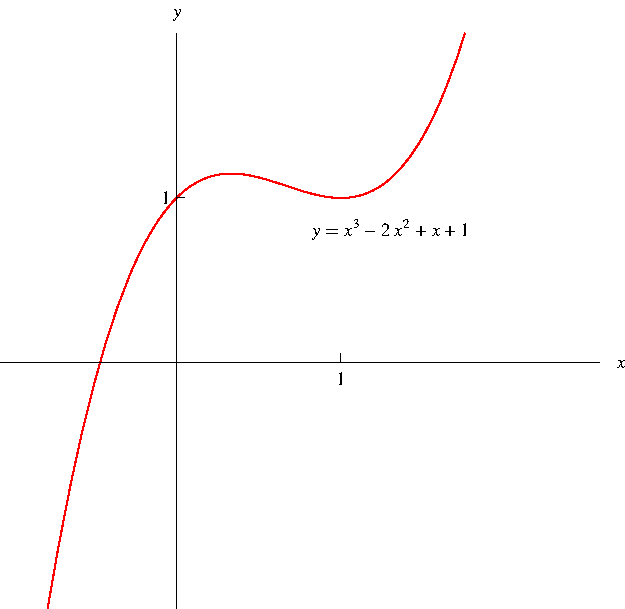
\includegraphics[height=6cm]{precalculus/pictures/01-02-polya.pdf}%

Cubic
}%
\only<handout:4| 4>{%
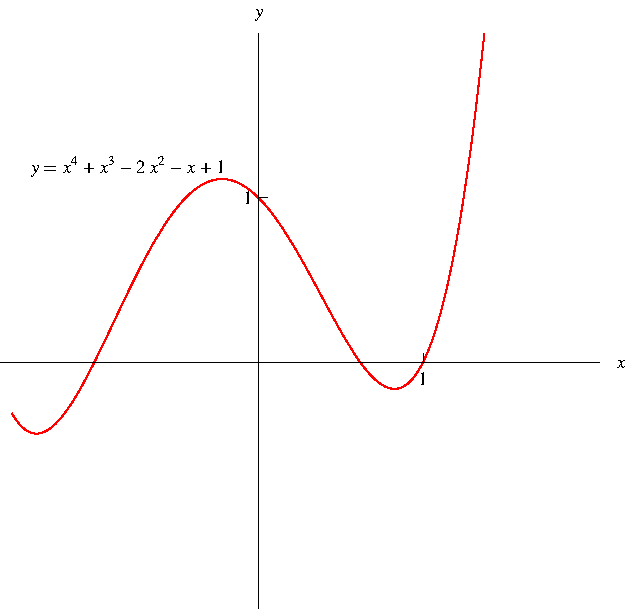
\includegraphics[height=6cm]{precalculus/pictures/01-02-polyb.pdf}%

Quartic
}%
\only<handout:5| 5>{%
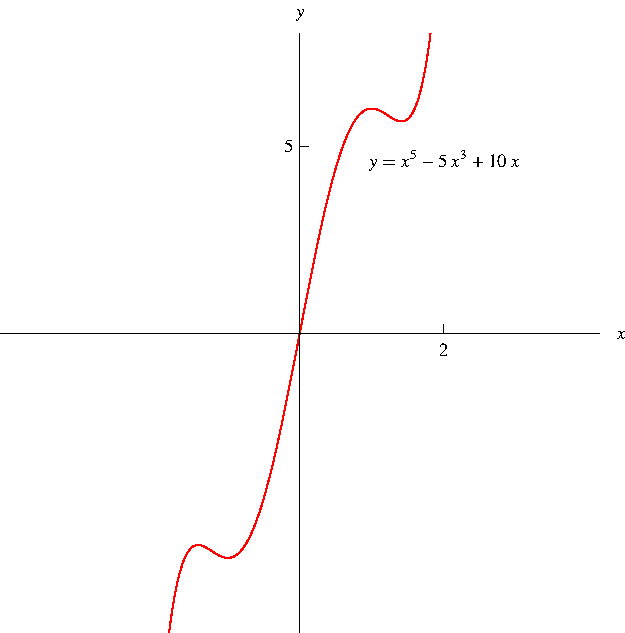
\includegraphics[height=6cm]{precalculus/pictures/01-02-polyc.pdf}%

Quintic
}
\end{frame}
% end module polynomials

% end lecture

% begin lecture
\lect{January 25, 2012}{Lecture  2}{2}
\section{(1.2) A Catalog of Essential Functions}
\subsection{Power Functions}
%Old Version from Greg. Greg, this slide is changed substantially, please take a look.
%% begin module power-functions-def
%\begin{frame}
%\frametitle{Power Functions}
%\begin{definition}[Power Function]
%A power function is a function of the form
%\[
%f(x) = x^a,
%\]
%where $a$ is a fixed real number.
%\end{definition}
%\uncover<2->{
%If $a$ is a positive integer like $1, 2, 3, \ldots$ then $x^a$ is a polynomial.

%\only<handout:-2| -2>{%
%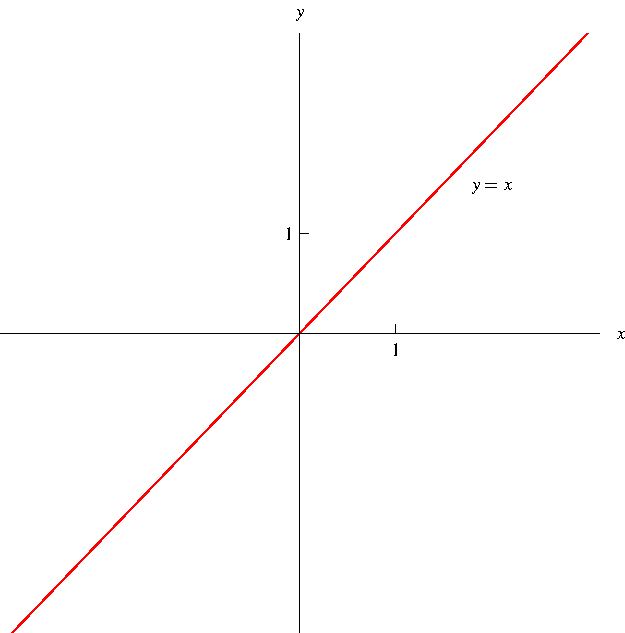
\includegraphics[height=4cm]{precalculus/pictures/01-02-x.pdf}%
%}%
%\only<handout:3| 3>{%
%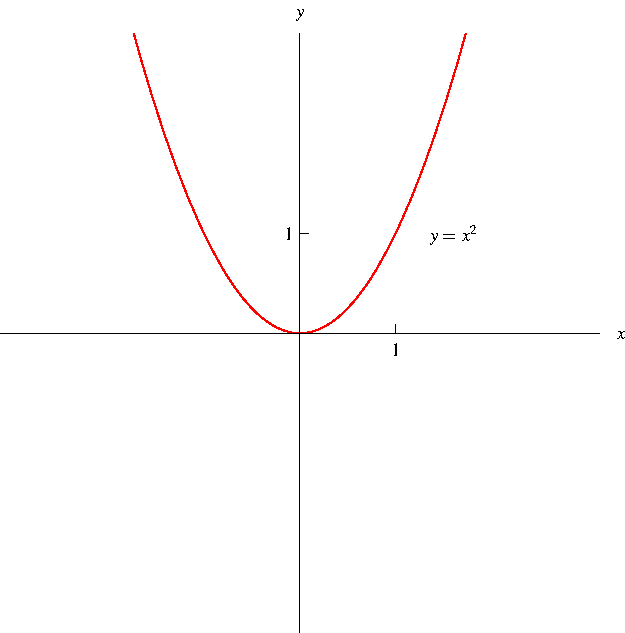
\includegraphics[height=4cm]{precalculus/pictures/01-02-xsquared.pdf}%
%}%
%\only<handout:4| 4>{%
%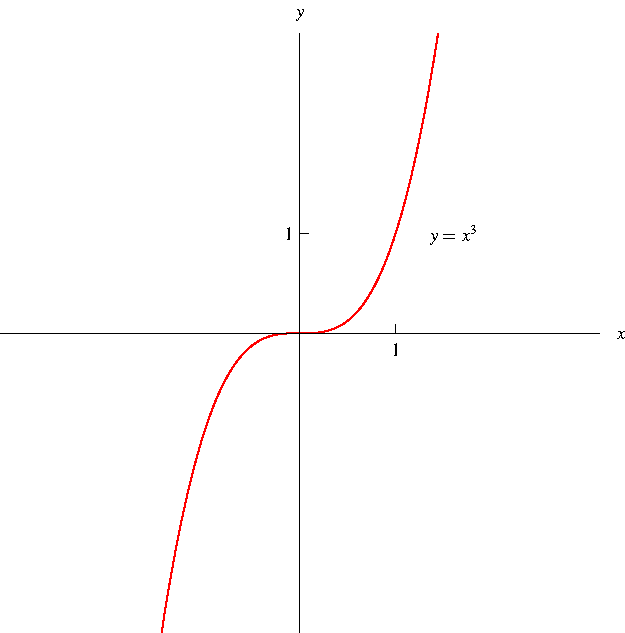
\includegraphics[height=4cm]{precalculus/pictures/01-02-xcubed.pdf}%
%}%
%\only<handout:5| 5>{%
%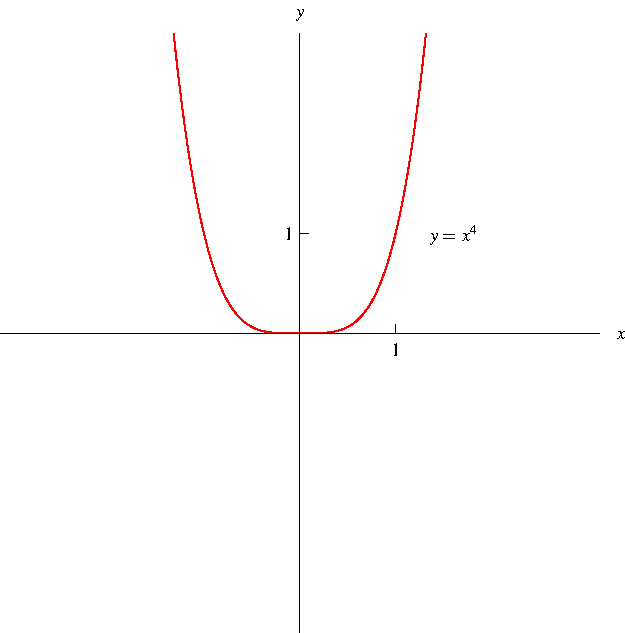
\includegraphics[height=4cm]{precalculus/pictures/01-02-xfourth.pdf}%
%}%
%\only<handout:6| 6>{%
%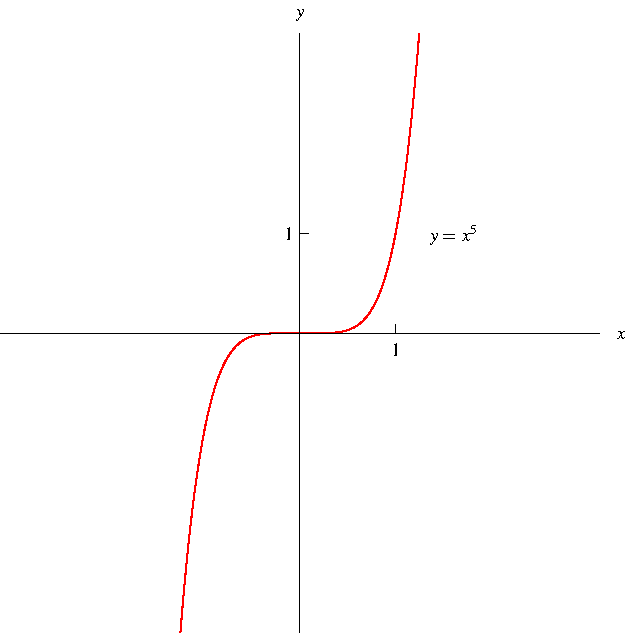
\includegraphics[height=4cm]{precalculus/pictures/01-02-xfifth.pdf}
%}%
%}%
%\end{frame}
%% end module power-functions-def

% begin module power-functions-def
\begin{frame}[t]
\frametitle{Power Functions}
\begin{definition}[Power Function]
Let $x>0$, $a$ - arbitrary real number. The power function is defined as
\[
f(x) \uncover<4->{\alertNoH{ 4}{=e^{a\ln x} } }= \alertNoH{2}{x}^{\alertNoH{3}{a}} \quad .
\]
\uncover<2->{$x$ = \alertNoH{2}{base}. } \uncover<3->{$a$ = \alertNoH{3}{exponent} or \alertNoH{3}{power}. }
\uncover<4->{\alertNoH{ 4}{First equality = one of ways to define for non-integer $a$ (we study $\ln x$, $e^x$ later). } }
\end{definition}
\begin{tabular}{@{}l}
\uncover<5->{
If $a$ - positive integer ($1, 2, 3, \ldots$) \\
then $x^a$ = polynomial function.
}\\
\uncover<5->{
$x^{n}    =\underbrace{x\dots x }_{n~\mathrm{times}}$ when $n$-integer. \\

$\begin{array}{rcl}
\alertNoH{12}{(x^{a})^b}&=&\fcAnswer{13}{x^{ab}}  \\
\alertNoH{14}{(xy)^b}   &=&\fcAnswer{15}{ x^by^b}\\
\alertNoH{16}{x^{a+b}}  &=&\fcAnswer{17}{x^ax^b } \\
\alertNoH{18}{x^{-a}}   &=&\fcAnswer{19}{\frac{1}{x^a}}
\end{array}
$\\
~\\~\\~\\~\\~\\~\\~\\
}
\end{tabular}
\uncover<6->{
\psset{xunit=0.38cm,yunit=0.38cm}
\begin{pspicture}(-5,-5)(5.4,5.2)
\psaxes[labels=none]{<->}(0,0)(-5,-5)(5,5)
\tiny
\rput[r](0,5){\tiny{$y$}}
\rput[l](5,0){\tiny{$x$}}
\only<handout:1|7>{
\psplot[linecolor=red]{-5}{5}{ x 1 exp }
\rput( 3, 1){$y=x^{\phantom{1}}$}
} %only
\only<handout:2|8>{
\psplot[linecolor=red]{-2.23}{2.23}{ x 2 exp }
\rput( 3, 1){$y=x^2$}
}
\only<handout:3|9>{
\psplot[linecolor=red]{-1.7}{1.7}{ x 3 exp }
\rput( 3, 1){$y=x^3$}
}
\only<handout:4|10>{
\psplot[linecolor=red]{-1.49}{1.49}{ x 4 exp }
\rput( 3, 1){$y=x^4$}
}
\only<handout:5|11->{
\psplot[linecolor=red]{-1.37}{1.37}{ x 5 exp }
\rput( 3, 1){$y=x^5$}
}
\end{pspicture}
\uncover<handout:5|11->{}
%\only<handout:-2| -2>{%
%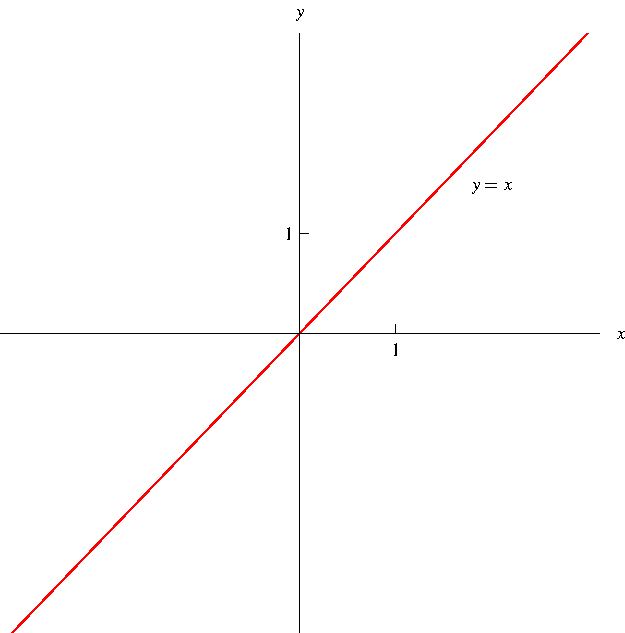
\includegraphics[height=4cm]{precalculus/pictures/01-02-x.pdf}%
%}%
%\only<handout:3| 3>{%
%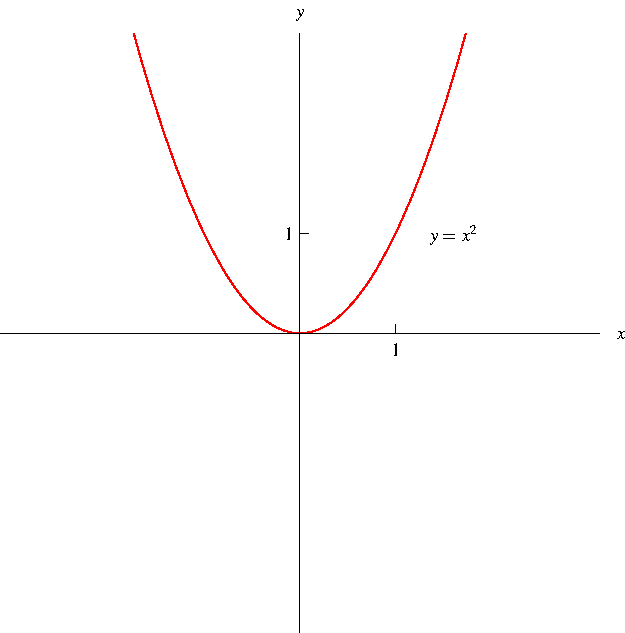
\includegraphics[height=4cm]{precalculus/pictures/01-02-xsquared.pdf}%
%}%
%\only<handout:4| 4>{%
%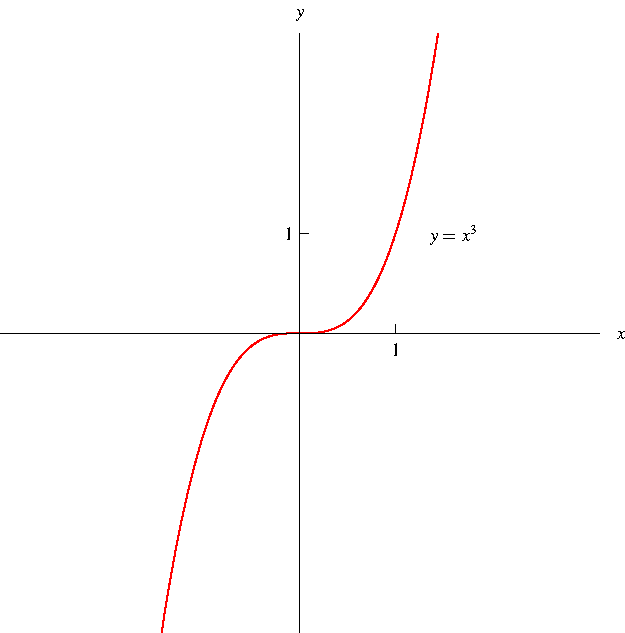
\includegraphics[height=4cm]{precalculus/pictures/01-02-xcubed.pdf}%
%}%
%\only<handout:5| 5>{%
%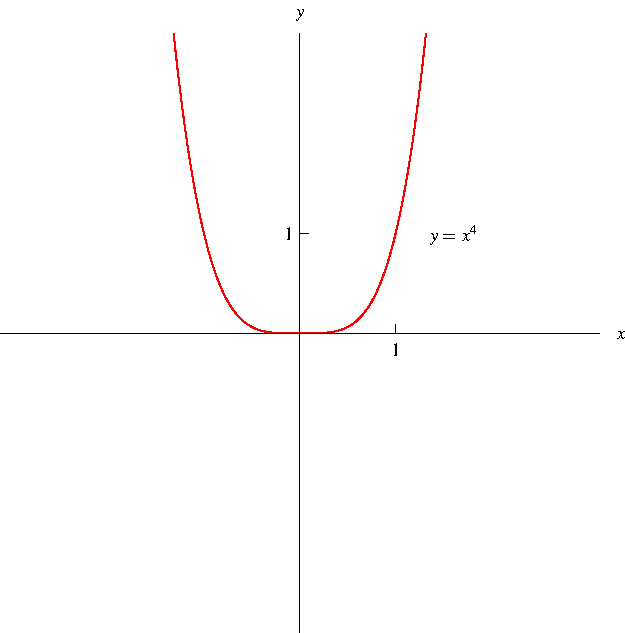
\includegraphics[height=4cm]{precalculus/pictures/01-02-xfourth.pdf}%
%}%
%\only<handout:6| 6>{%
%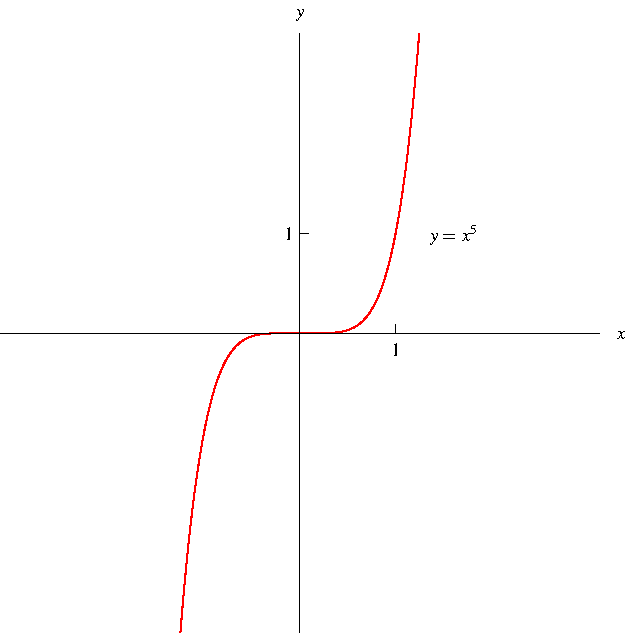
\includegraphics[height=4cm]{precalculus/pictures/01-02-xfifth.pdf}
%}%
}
\end{frame}
% end module power-functions-def

%Old Version from Greg. Greg, this slide is changed substantially, please take a look.
% begin module root-functions
%\begin{frame}
%\begin{itemize}
%\item<1->  If $n$ is a positive integer, the function $f(x) = x^{\frac{1}{n}} = \sqrt[n]{x}$ is called a root function.
%\item<2->  When $n = 2$, it is the square root function $f(x) = \sqrt{x}$.
%\item<3->  The square root is not defined for negative numbers, so its domain is $[0, \infty)$.
%\item<4->  Its graph is the top half of the parabola $x = y^2$.
%\item<5->  The graph of the cube root function $f(x) = \sqrt[3]{x}$ is similar to that of the square root, but it is defined everywhere.
%\end{itemize}
%\begin{tabular}{cc}
%\uncover<2->{%
%\includegraphics[height=3.5cm]{precalculus/pictures/01-02-sqrtx.pdf}%
%}%
%&%
%\uncover<5->{%
%\includegraphics[height=3.5cm]{precalculus/pictures/cube-root.pdf}%
%}%
%\end{tabular}
%\end{frame}
% end module root-functions

% begin module root-functions
\begin{frame}
\begin{itemize}
\item<1->  $n$ - positive integer, $f(x) = x^{\frac{1}{n}} = \sqrt[n]{x}$ = the $n^{th}$ root function. $\sqrt[n]{x}\geq 0$ for $x\geq 0$. 
\item<2->  For $n = 2$, we get the square root $\sqrt{x}$; for $n=3$ we get the cube root $\sqrt[3]{x}$, and so on. 
\item<3-> Let $x>0$. For $n=2m+1$-odd, we can extend the definition of $n^{th}$ root to negative numbers by $ \sqrt[2m+1]{-x}:= -\sqrt[2m+1]{x}$. 
\item<4-> In this course, even roots of negative numbers are not defined.
\item<5-> The graph of $\sqrt{x}$ is the top half of the parabola $x = y^2$. \uncover<6->{Similarly for $y=\sqrt[2m]{x}$, we graph top of $x=y^{2m}$.}
\item<7->  The graph of the cube root $f(x) = \sqrt[3]{x}$ is the graph of the polynomial $x=y^3$. \uncover<8->{Similarly for $y=\sqrt[2m+1]{x}$, we graph $x=y^{2m+1}$}.
\end{itemize}
\begin{tabular}{cc}
\uncover<5->{%
\psset{xunit=0.6cm,yunit=0.6cm}
\tiny
\begin{pspicture}(-3,-2)(3,2)
\psaxes[labels=none]{<->}(0,0)(-3,-2)(3,2)
\rput[r](0,2){{$y$}}
\rput[l](3,0){{$x$}}
\uncover<5>{
\psplot[linecolor=red]{0}{3}{ x 0.5 exp }
\rput( 3, 0.5){$y=\sqrt{x}$}
}
\uncover<6->{
\psplot[linecolor=red, plotpoints=300]{0}{3}{ x 0.25 exp }
\rput( 3, 0.5){$y=\sqrt[4]{x}$}
}
\end{pspicture}
%\uncover<2->{%
%\includegraphics[height=3.5cm]{precalculus/pictures/01-02-sqrtx.pdf}%
%}%
}%
&%
\uncover<7->{%
\psset{xunit=0.6cm,yunit=0.6cm}
\tiny
\begin{pspicture}(-3,-2)(3,2)
\psaxes[labels=none]{<->}(0,0)(-3,-2)(3,2)
\rput[r](0,2){\tiny{$y$}}
\rput[l](3,0){\tiny{$x$}}
\uncover<7>{
\psplot[linecolor=red, plotpoints=300]{-3}{0}{ x -1 mul 0.3333 exp -1 mul}
\psplot[linecolor=red, plotpoints=300]{0}{3}{ x         0.3333 exp }
\rput( 3, 0.5){$y=\sqrt[3]{x}$}
}
\uncover<8->{
\psplot[linecolor=red]{-3}{0}{ x -1 mul 0.2 exp -1 mul}
\psplot[linecolor=red]{0}{3}{ x         0.2 exp }
\rput( 3, 0.5){$y=\sqrt[5]{x}$}
}
\end{pspicture}
%\uncover<5->{%
%\includegraphics[height=3.5cm]{precalculus/pictures/cube-root.pdf}%
%}%
}%
\end{tabular}
\end{frame}
% end module root-functions
% begin module reciprocal-function
\begin{frame}
$f(x) = x^{-1} = \frac{1}{x}$ is called the reciprocal function.  Its graph has equation $y = \frac{1}{x}$, or $xy = 1$, and is an hyperbola with the coordinate axes as its asymptotes.
%\begin{center}%center does not work with well with pstricks and pgflayout.
\hfil\hfil\psset{xunit=0.6cm, yunit=0.6cm}
\begin{pspicture}(-5, -5)(5,5)
\psframe*[linecolor=white](-5,-5)(5,5)
\psaxes[ticks=none, labels=none]{<->}(0,0)(-5,-5)(5,5)\tiny
%Function formula: (1)/(x)
\rput(1,3){$y=\frac 1 x$}
\psplot[linecolor=red, plotpoints=1000]{0.2}{5}{1 x div } %Function formula: (1)/(x)
\rput(1,3){$y=\frac 1 x$}
\psplot[linecolor=red, plotpoints=1000]{-5}{-0.2}{1 x div }
\fcLabels{4.5}{4.5}
\end{pspicture}
%\includegraphics[height=5cm]{precalculus/pictures/reciprocal-function.pdf}%
%\end{center}
\end{frame}
% end module reciprocal-function

\subsection{Rational Functions}
% begin module rational-functions
\begin{frame}
\frametitle{Rational Functions}
\begin{definition}[Rational Function]
A rational function is a quotient of two polynomials; that is, a function of the form
\[
f(x) = \frac{g(x)}{h(x)},
\]
where $g$ and $h$ are polynomials.
\end{definition}
\begin{columns}[c]
\column{.4\textwidth}
\uncover<2->{
\psset{xunit=0.4cm, yunit=0.4cm}
\begin{pspicture}(-5, -5)(5,5)
\psframe*[linecolor=white](-5,-5)(5,5)
\psaxes[ticks=none, labels=none]{<->}(0,0)(-4.5,-4.5)(4.5,4.5)\tiny
%Function formula: \frac{x}{(x)^{2}-1}
\rput(2.5,-3){$y=\frac{x}{x^{2}-1}$}
\psplot[linecolor=red, plotpoints=1000]{1.11727}{4.5}{x -1 x 2 exp add div } %Function formula: \frac{x}{(x)^{2}-1}
\psplot[linecolor=red, plotpoints=1000]{-0.895043}{0.895043}{x -1 x 2 exp add div } %Function formula: \frac{x}{(x)^{2}-1}
\psplot[linecolor=red, plotpoints=1000]{-4.5}{-1.11727}{x -1 x 2 exp add div }
\fcLabels{4.5}{4.5}
\end{pspicture}
%\includegraphics[height=4cm]{precalculus/pictures/01-02-rational.pdf}%
}
\column{.6\textwidth}
\uncover<2->{
\begin{example}[$x/(x^2-1)$]
The function
\[
f(x) = \frac{x}{x^2-1}
\]
is a rational function.
\end{example}
}
\end{columns}
\end{frame}
% end module rational-functions

\subsection{Algebraic Functions}
%Old Version from Greg. Greg, this slide is changed substantially, please take a look.
%% begin module algebraic-functions
%\begin{frame}
%\frametitle{Algebraic Functions}
%\begin{definition}[Algebraic Function]
%An algebraic function is a function that can be constructed using algebraic operations (such as addition, subtraction, multiplication, division, and taking roots) starting from polynomials.
%\end{definition}
%\uncover<2->{
%Algebraic functions can look pretty funny.
%\begin{tabular}{ccc}
%\includegraphics[height=3.8cm]{precalculus/pictures/01-02-algebraic1.pdf}&%
%\includegraphics[height=3.8cm]{precalculus/pictures/01-02-algebraic2.pdf}&%
%\includegraphics[height=3.8cm]{precalculus/pictures/01-02-algebraic3.pdf}%
%\end{tabular}
%}
%\end{frame}
%% end module algebraic-functions


% begin module algebraic-functions
\begin{frame}
\frametitle{Algebraic Functions}
\begin{definition}[Algebraic Function]
A function in $x$ that can be constructed using $x$, constants, and finitely many of the operations $+, -, *, /,$ and $\sqrt[n]{~}$ is an algebraic function.

\uncover<2->{{\footnotesize Outside of Calculus I: function $f(x)$ = algebraic if it satisfies a polynomial equation with polynomial coefficients, i.e., $a_0(x) +a_1(x)f(x)+\dots +a_n(x) \left(f(x)\right)^n=0$ for some polynomials  $a_i(x)$.}}
\end{definition}
\uncover<3->{
Examples.

\begin{tabular}{ccc}
\psset{xunit=0.3cm, yunit=0.3cm}
\begin{pspicture}(-5, -5)(5,5) 
\tiny\psframe*[linecolor=white](-5,-5)(5,5) 
\psaxes[ticks=none, labels=none]{<->}(0,0)(-4.5,-4.5)(4.5,4.5)\tiny
%Function formula: - ((- (x))^{5/3})- ((- (x))^{2/3}) 
\psplot[linecolor=red, plotpoints=1000]{-2}{-0.001}{x -1 mul 0.666667 exp -1 mul x -1 mul 1.66667 exp -1 mul add } %Function formula: (x)^{5/3}- ((x)^{2/3}) 
\rput[t](1,-5){$y=(x-1)\sqrt[3]{x^2}$} 
\psplot[linecolor=red, plotpoints=1000]{0.001}{3}{x 0.666667 exp -1 mul x 1.66667 exp add }
\psLabels{4.5}{4.5}
\end{pspicture} 
%\includegraphics[height=3.8cm]{precalculus/pictures/01-02-algebraic1.pdf}
&%
\psset{xunit=0.3cm, yunit=0.3cm}
\begin{pspicture}(-5, -5)(5,5) 
\tiny\psframe*[linecolor=white](-5,-5)(5,5) 
\psaxes[ticks=none, labels=none]{<->}(0,0)(-4.5,-4.5)(4.5,4.5)\tiny
\psplot[linecolor=red, plotpoints=1000]{1}{5}{-1 x 2 exp add 0.5 exp x 2 exp mul -0.2 mul -1 x 2 exp add 0.5 exp x mul 0.8 mul add } %Function formula: 4/5 ((x) (((x)^{2}-1)^{1/2}))-1/5 (((x)^{2}) (((x)^{2}-1)^{1/2})) 
\rput[t](1,-5){$y=\frac15(4x-x^2)\sqrt{x^2-1}$} 
\psplot[linecolor=red, plotpoints=1000]{-2}{-1}{-1 x 2 exp add 0.5 exp x 2 exp mul -0.2 mul -1 x 2 exp add 0.5 exp x mul 0.8 mul add }
\psLabels{4.5}{4.5}
\end{pspicture} 
%\includegraphics[height=3.8cm]{precalculus/pictures/01-02-algebraic2.pdf}
&%
\psset{xunit=0.3cm, yunit=0.3cm}
\begin{pspicture}(-5, -5)(5,5) 
\tiny\psframe*[linecolor=white](-5,-5)(5,5) 
\psaxes[ticks=none, labels=none]{<->}(0,0)(-4.5,-4.5)(4.5,4.5)\tiny
%Function formula: - ((4- ((x)^{2}))^{1/2})+(x) ((4- ((x)^{2}))^{1/2}) 
\rput[t](1,-5){$y=(x-1)\sqrt{4-x^2}$} 
\psplot[linecolor=red, plotpoints=1000]{-2}{2}{x 2 exp -1 mul 4 add 0.5 exp x mul x 2 exp -1 mul 4 add 0.5 exp -1 mul add }
\psLabels{4.5}{4.5}
\end{pspicture} 
%\includegraphics[height=3.8cm]{precalculus/pictures/01-02-algebraic3.pdf}
%
\end{tabular}
}
\end{frame}
% end module algebraic-functions

\subsection{Transcendental Functions}
% begin module transcendental-functions
\begin{frame}
\frametitle{Transcendental Functions}
The set of transcendental functions includes several classes of functions.
\begin{itemize}
\item<2->  Trigonometric functions such as $\cos x, \sin x, \tan x,$ etc.
\item<3->  Exponential functions such as $2^x, \left( \frac{1}{2}\right)^x, 5^x, e^x$, etc.
\item<4->  Logarithmic functions such as $\log_2x, \log_{10}x, \ln x$, etc.
\item<5->  Many other functions that don't even have names.
\end{itemize}
\end{frame}
% end module transcendental-functions 

\section{(1.3) New Functions from Old Functions}
\subsection{Transformations of Functions}
% begin module transformations-shifts
\begin{frame}
\frametitle{Transformations of Functions}
\begin{columns}[c]
\column{.5\textwidth}

\psset{xunit=1cm, yunit=1cm}
\begin{pspicture}(-5, -5)(5,5) 
\tiny 
\psframe*[linecolor=white](-5,-5)(5,5) 
\psaxes[ticks=none, labels=none]{<->}(0,0)(-0.5,-0.5)(4.5,4.5)
\rput[t](4.5, -0.1){$x$}
\rput[r](-0.1, 4.5){$y$}
%Function formula: 10/3+1/3 ((-3+3 (x))^{3})-1/3 ((-3+3 (x))^{2})-1/3 (x) 

\only<handout:0| -2>{
\psplot[linecolor=red, plotpoints=1000]{1.65}{2.55}{x -0.333333 mul x 3 mul -6 add 2 exp -0.333333 mul x 3 mul -6 add 3 exp 0.333333 mul 2.66667 add add add }
\rput[b] (2.55, 2.40654){\alert<-2>{$y=f(x)$}}
}
\only<handout:0| 3->{
\psplot[linecolor=blue, plotpoints=1000]{1.65}{2.55}{x -0.333333 mul x 3 mul -6 add 2 exp -0.333333 mul x 3 mul -6 add 3 exp 0.333333 mul 2.66667 add add add }
\rput[b] (2.55, 2.40654){$y=f(x)$}
}

\only<handout:0| 3>{%
\psplot[linecolor=red, plotpoints=1000]{1.65}{2.55}{x -0.333333 mul x 3 mul -6 add 2 exp -0.333333 mul x 3 mul -6 add 3 exp 0.333333 mul 4.16667 add add add }
\rput[b](2.55, 3.90654){\alert<3>{$y=f(x)+c$}}
}
\only<handout:0| 4->{%
\psplot[linecolor=blue, plotpoints=1000]{1.65}{2.55}{x -0.333333 mul x 3 mul -6 add 2 exp -0.333333 mul x 3 mul -6 add 3 exp 0.333333 mul 4.16667 add add add }
\rput[b](2.55, 3.90654){$y=f(x)+c$}
}


\only<handout:0| 4>{%
\psplot[linecolor=red, plotpoints=1000]{1.65}{2.55}{x -0.333333 mul x 3 mul -6 add 2 exp -0.333333 mul x 3 mul -6 add 3 exp 0.333333 mul 1.16667 add add add }
\rput[b](2.55, 0.906542){$y=f(x)-c$}
}
\only<handout:0| 5->{%
\psplot[linecolor=blue, plotpoints=1000]{1.65}{2.55}{x -0.333333 mul x 3 mul -6 add 2 exp -0.333333 mul x 3 mul -6 add 3 exp 0.333333 mul 1.16667 add add add }
\rput[b](2.55, 0.906542){$y=f(x)-c$}
}

\only<handout:0| 5>{%
\psplot[linecolor=red, plotpoints=1000]{3.15}{4.05}{x -0.333333 mul x 3 mul -10.5 add 2 exp -0.333333 mul x 3 mul -10.5 add 3 exp 0.333333 mul 3.16667 add add add }
\rput[b](4.05, 2.40654){\alert<5>{$y=f(x-c)$}}
}
\only<handout:0| 6->{%
\psplot[linecolor=blue, plotpoints=1000]{3.15}{4.05}{x -0.333333 mul x 3 mul -10.5 add 2 exp -0.333333 mul x 3 mul -10.5 add 3 exp 0.333333 mul 3.16667 add add add }
\rput[b](4.05, 2.40654){$y=f(x-c)$}
}

\only<6>{%
\psplot[linecolor=red, plotpoints=1000]{0.15}{1.05}{x -0.333333 mul x 3 mul -1.5 add 2 exp -0.333333 mul x 3 mul -1.5 add 3 exp 0.333333 mul 2.16667 add add add }
\rput[b](1.05, 2.40654){\alert<6>{$y=f(x+c)$}}
}
\end{pspicture} 
%\ \only<handout:0| -2>{%
%\includegraphics[height=5cm]{precalculus/pictures/01-03-shifta.pdf}%
%}%
%\only<handout:0| 3>{%
%\includegraphics[height=5cm]{precalculus/pictures/01-03-shiftb.pdf}%
%}%
%\only<handout:0| 4>{%
%\includegraphics[height=5cm]{precalculus/pictures/01-03-shiftc.pdf}%
%}%
%\only<handout:0| 5>{%
%\includegraphics[height=5cm]{precalculus/pictures/01-03-shiftd.pdf}%
%}%
%\only<6>{%
%\includegraphics[height=5cm]{precalculus/pictures/01-03-shifte.pdf}%
%}%a
\column{.5\textwidth}
What happens if we add or subtract a positive constant $c$ in the equation of a function $f$?  What happens if we add or subtract $c$ from $x$ before applying the function $f$?
\end{columns}

\uncover<2->{
\begin{tabular}{|l|l|}
\hline
\alert<handout:0| 3>{$f(x)+c$} &%
\uncover<3->{\alert<handout:0| 3>{Shift the graph of $f(x)$ $c$ units up.}} \\%
\alert<handout:0| 4>{$f(x)-c$} &%
\uncover<4->{\alert<handout:0| 4>{Shift the graph of $f(x)$ $c$ units down.}} \\%
\alert<handout:0| 5>{$f(x-c)$} &%
\uncover<5->{\alert<handout:0| 5>{Shift the graph of $f(x)$ $c$ units right.}} \\%
\alert<handout:0| 6>{$f(x+c)$} &%
\uncover<6->{\alert<handout:0| 6>{Shift the graph of $f(x)$ $c$ units left.}}\\%
\hline
\end{tabular}
}
\end{frame}
% end module transformations-shifts
% begin module transformations-shifts-example
\begin{frame}
\begin{example}[Example 2, p. 39]
Draw a graph of the function $f(x) = x^2 + 6x + 10$.
\begin{columns}[c]
\column{.5\textwidth}
\ \only<handout:0| -6>{%
\includegraphics[height=5cm]{precalculus/pictures/01-03-parabolaa.pdf}%
}%
\only<handout:0| 7>{%
\includegraphics[height=5cm]{precalculus/pictures/01-03-parabolab.pdf}%
}%
\only<8->{%
\includegraphics[height=5cm]{precalculus/pictures/01-03-parabolac.pdf}%
}%
\column{.5\textwidth}
\uncover<2->{
Complete the square:
}
\begin{eqnarray*}
\uncover<3->{f(x)} & \uncover<3->{ = } & \uncover<3->{x^2 + 6x + 10} \\
& \uncover<4->{ = } & \uncover<4->{(x^2 + 6x \uncover<5->{\alert<handout:0| 5>{+ 9}}) + 10 \uncover<5->{\alert<handout:0| 5>{- 9}}} \\
 & \uncover<6->{ = } & \uncover<6->{(x + 3)^2 + 1} \\
\end{eqnarray*}
\end{columns}
\end{example}
\end{frame}
% end module transformations-shifts-example

% begin module transformations-magnifications
\begin{frame}
\begin{columns}[c]
\column{.5\textwidth}

\psset{xunit=0.7cm, yunit=0.7cm}
\begin{pspicture}(-4, -3.5)(4.5,5)
\tiny
\fcAxesStandard{-4}{-3.5}{4.5}{5}
%Function formula: 10/3+1/3 ((-3+3 (x))^{3})-1/3 ((-3+3 (x))^{2})-1/3 (x)
\only<handout:1| 1->{
\psplot[linecolor=red, plotpoints=1000]{1.65}{2.55}{x -0.333333 mul x 3 mul -6 add 2 exp -0.333333 mul x 3 mul -6 add 3 exp 0.333333 mul 2.66667 add add add }
\rput[b] (2.55, 2.40654){$y=f(x)$}
}
%\only<handout:0| 3->{
%\psplot[linecolor=blue, plotpoints=1000]{1.65}{2.55}{x -0.333333 mul x 3 mul %-6 add 2 exp -0.333333 mul x 3 mul -6 add 3 exp 0.333333 mul 2.66667 add add %add }
%\rput[b] (2.55, 2.40654){$y=f(x)$}
%}

\only<handout:0| 3>{
\psplot[linecolor=red, plotpoints=1000]{1.65}{2.55}{x -0.333333 mul x 3 mul -6 add 2 exp -0.333333 mul x 3 mul -6 add 3 exp 0.333333 mul 2.66667 add add add 2 mul}
\rput[b] (2.55, 4.80654){{$y=cf(x)$}}
}
\only<handout:1| 4->{
\psplot[linecolor=blue, plotpoints=1000]{1.65}{2.55}{x -0.333333 mul x 3 mul -6 add 2 exp -0.333333 mul x 3 mul -6 add 3 exp 0.333333 mul 2.66667 add add add 2 mul}
\rput[b] (2.55, 4.80654){$y=cf(x)$}
}

\only<handout:0| 4>{
\psplot[linecolor=red, plotpoints=1000]{1.65}{2.55}{x -0.333333 mul x 3 mul -6 add 2 exp -0.333333 mul x 3 mul -6 add 3 exp 0.333333 mul 2.66667 add add add 2 div}
\rput[b] (2.55, 0.40654){{$y=\frac{1}{c}f(x)$}}
}
\only<handout:1| 5->{
\psplot[linecolor=blue, plotpoints=1000]{1.65}{2.55}{x -0.333333 mul x 3 mul -6 add 2 exp -0.333333 mul x 3 mul -6 add 3 exp 0.333333 mul 2.66667 add add add 2 div}
\rput[b] (2.55, 0.40654){$y=\frac{1}{c}f(x)$}
}

\only<handout:0| 5>{
\psplot[linecolor=red, plotpoints=1000]{1.65}{2.55}{x -0.333333 mul x 3 mul -6 add 2 exp -0.333333 mul x 3 mul -6 add 3 exp 0.333333 mul 2.66667 add add add -1 mul}
\rput[t] (2.55, -2.40654){{$y=-f(x)$}}
}
\only<handout:1| 6->{
\psplot[linecolor=blue, plotpoints=1000]{1.65}{2.55}{x -0.333333 mul x 3 mul -6 add 2 exp -0.333333 mul x 3 mul -6 add 3 exp 0.333333 mul 2.66667 add add add -1 mul}
\rput[t] (2.55, -2.40654){$y=-f(x)$}
}

\only<handout:0| 6>{
%Function formula: 8/3+1/3 ((-6-3 (x))^{3})+1/3 (x)-1/3 ((-6-3 (x))^{2})
\psplot[linecolor=red, plotpoints=1000]{-2.55}{-1.65}{x -3 mul -6 add 2 exp -0.333333 mul x 0.333333 mul x -3 mul -6 add 3 exp 0.333333 mul 2.66667 add add add }
\rput[b] (-2.55, 2.40654){{$y=f(-x)$}}
}
\only<handout:1| 7->{
%Function formula: 8/3+1/3 ((-6-3 (x))^{3})+1/3 (x)-1/3 ((-6-3 (x))^{2})
\psplot[linecolor=blue, plotpoints=1000]{-2.55}{-1.65}{x -3 mul -6 add 2 exp -0.333333 mul x 0.333333 mul x -3 mul -6 add 3 exp 0.333333 mul 2.66667 add add add }
\rput[b] (-2.55, 2.40654){$y=f(-x)$}
}
\end{pspicture}
%\ \only<handout:0| -2>{%
%\includegraphics[height=5cm]{precalculus/pictures/01-03-maga.pdf}%
%}%
%\only<handout:0| 3>{%
%\includegraphics[height=5cm]{precalculus/pictures/01-03-magb.pdf}%
%}%
%\only<handout:0| 4>{%
%\includegraphics[height=5cm]{precalculus/pictures/01-03-magc.pdf}%
%}%
%\only<handout:0| 5>{%
%\includegraphics[height=5cm]{precalculus/pictures/01-03-magd.pdf}%
%}%
%\only<6>{%
%\includegraphics[height=5cm]{precalculus/pictures/01-03-mage.pdf}%
%}%

\column{.5\textwidth}
\alertNoH{3-4}{What happens if we multiply or divide by a constant $c > 1$ in the equation of a function $f$?}  \alertNoH{5}{What happens if we multiply $f$ by $-1$?}  \alertNoH{6}{What happens if we multiply $x$ by $-1$ before applying $f$?}
\end{columns}

\begin{tabular}{|l|l|}
\hline
\alert<handout:0| 3>{$cf(x)$} &%
\uncover<3->{\alert<handout:0| 3>{Stretch the graph of $f(x)$ vertically by a factor of $c$.}} \\%
\alert<handout:0| 4>{$(1/c)f(x)$} &%
\uncover<4->{\alert<handout:0| 4>{Compress the graph of $f(x)$ vertically by a factor of $c$.}} \\%
\alert<handout:0| 5>{$-f(x)$} &%
\uncover<5->{\alert<handout:0| 5>{Reflect the graph of $f(x)$ in the $x$-axis.}} \\%
\alert<handout:0| 6>{$f(-x)$} &%
\uncover<6->{\alert<handout:0| 6>{Reflect the graph of $f(x)$ in the $y$-axis.}}\\%
\hline
\end{tabular}
\uncover<7>{~} %this line is needed to avoid a latexing bug: without this line, the next slide will be messed up.

\end{frame}
% end module transformations-magnifications

% begin module transformations-horizontal-stretches
\begin{frame}\ %
\uncover<1->{}
\psset{xunit=1.4cm, yunit=1.4cm}
\begin{pspicture}(-0.6, -1.4)(6.2,1.4)
\tiny
\fcAxesStandard{-0.6}{-1.4}{6.2}{1.4}

%Function formula: sin{}(x)
\rput[t](4.71238898, -1.1){\alertNoH{1-2}{$y=sin{}(x)$}}

\uncover<1-2>{
\psplot[linecolor=red, plotpoints=1000]{-0.5}{6}{x 57.29578 mul sin }
}
\uncover<3->{
\psplot[linecolor=blue, plotpoints=1000]{-0.5}{6}{x 57.29578 mul sin }
}

\psline(1.570796327, -0.05)(1.570796327, 0.05)
\rput[t](1.570796327, -0.1) {$\frac{\pi}{2}$}

\psline(3.141592654, -0.05)(3.141592654, 0.05)
\rput[t](3.141592654, -0.1) {$\pi$}


\uncover<3->{
 %Function formula: sin{}(3/2 (x))
\uncover<3>{
\psplot[linecolor=red, plotpoints=1000]{-0.5}{6}{x 1.5 mul 57.29578 mul sin }
}
\uncover<4->{
\psplot[linecolor=blue, plotpoints=1000]{-0.5}{6}{x 1.5 mul 57.29578 mul sin }
}
\rput(3.141592654, -1.1){\alertNoH{3}{$y=\sin{}(cx)$}}

\psline(1.047197551, -0.05)(1.047197551, 0.05)
\rput[t](1.047197551, -0.1) {$\frac{\pi}{2c}$}

\psline(2.094395102, -0.05)(2.094395102, 0.05)
\rput[t](2.094395102, -0.1) {$\frac{\pi}{c}$}

}
\uncover<4->{
\rput[b](3.14,1.1){\alertNoH{4}{$y=\sin\left(\frac{x}{c}\right)$}}
\psplot[linecolor=red, plotpoints=1000]{-0.5}{6}{x 0.666667 mul 57.29578 mul sin }

\psline(2.35619449, -0.05)(2.35619449, 0.05)
\rput[t](2.35619449, -0.1) {$\frac{\pi c}{2}$}

\psline(4.71238898, -0.05)(4.71238898, 0.05)
\rput[t](4.71238898, -0.1) {$\pi c$}
}
\end{pspicture}
%\includegraphics[height=6cm]{precalculus/pictures/01-03-stretcha.pdf}%
%}%
%\only<handout:0| 3>{%
%\includegraphics[height=6cm]{precalculus/pictures/01-03-stretchb.pdf}%
%}%
%\only<4->{%
%\includegraphics[height=6cm]{precalculus/pictures/01-03-stretchc.pdf}%
%}%a

What happens if we multiply or divide $x$ by a constant $c > 1$ before applying $f$?

\uncover<2->{
\begin{tabular}{|l|l|}
\hline
\alert<handout:0| 3>{$f(cx)$} &%
\uncover<3->{\alert<handout:0| 3>{Compress the graph of $f(x)$ horizontally by a factor of $c$.}} \\%
\alert<handout:0| 4>{$f((1/c)x)$} &%
\uncover<4->{\alert<handout:0| 4>{Stretch the graph of $f(x)$ horizontally by a factor of $c$.}} \\%
\hline
\end{tabular}
}
\end{frame}
% end module transformations-horizontal-stretches

% begin module transformations-absolute-value
\begin{frame}
What happens when we take the absolute value of a function?
\uncover<2->{
\[
|f(x)| = \left\{ \begin{array}{rcc}
f(x) & \textrm{if} & f(x) \geq 0\\
-f(x) & \textrm{if} & f(x) < 0
\end{array}\right.
\]
}
\uncover<3->{%
This tells us how to draw the graph of $y = |f(x)|$: the part of the graph above the $x$-axis remains the same; the part below the $x$-axis is reflected about the $x$-axis.
}
\uncover<4->{
\begin{example}[Example 5, p. 41]
Draw the graph of the function $f(x) = |x^2 - 1|$.
\begin{columns}[c]
\column{.4\textwidth}
\ \only<handout:0| -4>{%
\includegraphics[height=4cm]{precalculus/pictures/01-03-ex5z.pdf}%
}%
\only<handout:0| 5>{%
\includegraphics[height=4cm]{precalculus/pictures/01-03-ex5a.pdf}%
}%
\only<handout:0| 6>{%
\includegraphics[height=4cm]{precalculus/pictures/01-03-ex5b.pdf}%
}%
\only<7->{%
\includegraphics[height=4cm]{precalculus/pictures/01-03-ex5c.pdf}%
}%
\column{.6\textwidth}
\begin{itemize}
\item<5->  Draw the graph of $f(x) = x^2 - 1$.
\item<6->  Identify the part(s) below the $x$-axis.
\item<7->  Flip those parts over the $x$-axis.
\end{itemize}
\end{columns}
\end{example}
}
\end{frame}
% end module transformations-absolute-value

\subsection{Combinations of Functions}
% begin module combinations-functions
\begin{frame}
\frametitle{Combinations of Functions}
Two functions $f$ and $g$ can be combined to form new functions $f+g$, $f-g$, $fg$, and $f/g$.  The sum and difference functions are defined by the formulas
\[
(f+g)(x) = f(x) + g(x), \qquad (f-g)(x) = f(x)-g(x).
\]
If $A$ is the domain of $f$ and $B$ is the domain of $g$, then the domain of $f+g$ and $f-g$ is $A\cap B$, the intersection of $A$ and $B$.

The product and quotient functions are defined by the formulas
\[
(fg)(x) = f(x)g(x), \qquad \left( \frac{f}{g}\right)(x) = \frac{f(x)}{g(x)}.
\]
These functions also have the domain $A\cap B$, with one exception: in the quotient function, we aren't allowed to divide by 0, so we must exclude those values of $x$ that make $g(x) = 0$.  We write this domain as
\[
\{ x\in A\cap B | \ g(x) \neq 0\} .
\]
\end{frame}
% end module combinations-functions

% begin module composition-functions
\begin{frame}
\begin{definition}[Composition of $f$ and $g$]
If $f$ and $g$ are two functions, then the composition of $f$ and $g$ is written $f\circ g$ and is defined by the formula
\[
(f\circ g)(x) = f(g(x)).
\]
\end{definition}

Imagine $f$ and $g$ as machines taking some input and producing some output. Then $f\circ g$ corresponds to attaching both machines end-to-end so that the output of $g$ becomes the input of $f$.

\psset{xunit=0.75cm, yunit=0.75cm}
\begin{pspicture}(-4, -2.5)(13,2.5) 
\footnotesize
\rput[r] (-3.1, 0){$x$}
\psline[linewidth=3pt]{->}(-3,0)(-2.25,0)

\rput(0.25,0){
\psMachine{$g$}{blue}
}
\rput (4, 0){$g(x)$}
\psline[linewidth=3pt]{->}(2.75,0)(3.5,0)
\psline[linewidth=3pt]{->}(4.5,0)(5.25,0)
\rput(7.75,0){
\psMachine{$f$}{red}
}
\rput (11.75, 0){$f(g(x))$}
\psline[linewidth=3pt]{->}(10.25,0)(11,0)
\end{pspicture} 
%\includegraphics[height=2cm]{precalculus/pictures/01-03-machines.pdf}%

\uncover<2->{
The domain of $f\circ g$ is the set of all numbers $x$ in the domain of $g$ such that $g(x)$ is in the domain of $f$.  If the domain of $f$ is $A$ and the domain of $g$ is $B$, we write this as
\[
\{ x\in B |\ g(x) \in A\} .
\]
}
\end{frame}
% end module composition-functions
% begin module composition-example
\begin{frame}
\begin{example}
Find $\alertNoH{2}{f\circ g},\alertNoH{14}{g\circ f}, \alertNoH{27}{g\circ g}$ and their domains, where \alertNoH{10,16}{$\alertNoH{5}{ f(} \alertNoH{6}{ x} \alertNoH{5}{) =}\only<handout:0|5> {\color{red}} \sqrt{\only<handout:0|5>{\color{black}} \alertNoH{6}{x}}$} and \alertNoH{4,29}{$\alertNoH{17,30}{ g(}\alertNoH{18,31}{ x} \alertNoH{17,30}{) = }\only<handout:0|17,30>{\color{red}} \sqrt{3 - \only<handout:0|17,30>{ \color{black}} \alertNoH{18,31}{x} }$}.

$
\begin{array}{rclll}
\only<handout:1|1-26>{%
\uncover<2->{\alertNoH{3}{ (\alertNoH{2}{f\circ g})(x)}} &\uncover<3->{ \alertNoH{3}{ =}} & \uncover<3->{\alertNoH{3}{ f(\alertNoH{4}{g(x)})}} \uncover<4->{ =\only<handout:0|5>{\color{red}} f\left( \only<handout:0|5>{ \color{black}}   \alertNoH{4,6}{\sqrt{3 - x}} \only<handout:0|5>{\color{red}} \right)} \uncover<5->{ = \only<handout:0|5>{ \color{red}}  \alertNoH{7}{\sqrt{ \only<handout:0|5>{ \color{black}} \alertNoH{6}{\sqrt{3-x}}}}} \uncover<7->{  \alertNoH{7}{= \sqrt[4]{\alertNoH{7,9}{ 3-x} }}}\\
\uncover<8->{\text{Domain: }}\\
\uncover<9->{\alertNoH{9}{\alertNoH{10}{3}-x}&\alertNoH{9}{\geq} & \alertNoH{9}{0}} \\ 
\uncover<10->{\alertNoH{11}{-}x&\alertNoH{11}{\geq} & \alertNoH{10}{ \alertNoH{11}{-} 3}}\\
\uncover<11->{\alertNoH{13}{x}&\alertNoH{11,13}{\leq}&\alertNoH{13}{ 3} }\\
\uncover<12->{\alertNoH{12,13}{x} &\alertNoH{12,13}{\in}& \fcAnswer{13}{(-\infty , 3].}}\\
\uncover<14->{\alertNoH{15}{ (\alertNoH{14}{g\circ f})(x)}}& \uncover<15->{ \alertNoH{15}{=} } & \uncover<15->{ \alertNoH{15}{ g(\alertNoH{16}{ f(x)})}}
\uncover<16->{ = \alertNoH{17}{g(}\alertNoH{16,18}{\sqrt{x}}\alertNoH{17}{)}} \uncover<17->{ = \only<handout:0|17>{\color{red}}  \sqrt{\alertNoH{21}{ 3 - \only<handout:0|17>{ \color{black}} \alertNoH{18}{\sqrt{\alertNoH{20}{x}} }} }}\\
\uncover<19->{\text{Domain}:}\\
\uncover<20->{\alertNoH{20,26}{x}&\alertNoH{20,26}{\geq} & \alertNoH{20,26}{0} }\\
\uncover<21->{\alertNoH{21}{\alertNoH{22}{ 3} - \sqrt{x}}& \alertNoH{21}{ \geq } & \alertNoH{21}{ 0} }\\
\uncover<22->{ \alertNoH{23}{-} \sqrt{x} &\alertNoH{23}{\geq }& \alertNoH{22}{ \alertNoH{23}{-}3 }}\\
\uncover<23->{\sqrt{x}&\alertNoH{23}{ \leq} & 3} \\
\uncover<24->{\alertNoH{26}{ x}& \alertNoH{26}{ \alertNoH{0}{\leq}} &\alertNoH{26}{ 9}}\\
\uncover<25->{ \alertNoH{25,26}{x}&\alertNoH{25,26}{\in}& \fcAnswer{26}{[0,9]}} \\
}%only<handout:1|1->  
\only<handout:2|27->{%
\uncover<27->{\alertNoH{28}{ (\alertNoH{27}{g\circ g})(x)}} & \uncover<28->{ \alertNoH{28} {=} } & \uncover<28->{\alertNoH{28}{ g( \alertNoH{29 }{ g(x)})}} \uncover<29->{ = \only<handout:0|30>{\color{red}}  g \left( \only<handout:0|30>{ \color{black}} \alertNoH{29}{\sqrt{3 - x}}  \only<handout:0|30>{\color{red}} \right)}  \uncover<30->{ \only<handout:0|30>{\color{red}} = \sqrt{\alertNoH{36}{ 3 - \only<handout:0|30>{\color{black}}\alertNoH{31}{\sqrt{\alertNoH{33}{3-x} } }}}}\\
\uncover<32->{\text{Domain}:}\\
\uncover<33->{\alertNoH{33}{\alertNoH{34} {3}-x} & \alertNoH{33}{\geq} &\alertNoH{33}{ 0}}\\
\uncover<34->{\alertNoH{35}{-}x&\alertNoH{35}{\geq} & \alertNoH{34}{ \alertNoH{35}{ - } 3}}\\ 
\uncover<35->{\alertNoH{43}{x}&\alertNoH{35,43}{\leq} &\alertNoH{43}{ 3}}\\ 
\uncover<36->{\alertNoH{36}{\alertNoH{37}{3}-\sqrt{3-x}}&\alertNoH{36}{\geq }&\alertNoH{36}{ 0}} \\
\uncover<37->{\alertNoH{38}{-}\sqrt{3-x}&\alertNoH{38}{\geq}& \alertNoH{37}{\alertNoH{38}{-} 3}}\\
\uncover<38->{\sqrt{3-x}&\alertNoH{38}{\leq}& 3} \\
\uncover<39->{\alertNoH{40}{3}-x&\alertNoH{0}{\leq} &\alertNoH{40}{ 9}}\\
\uncover<40->{\alertNoH{41}{-}x&\alertNoH{41}{\leq}& \alertNoH{40}{6}}\\
\uncover<41->{\alertNoH{43}{x}&\alertNoH{41,43}{\geq}& \alertNoH{43}{ \alertNoH{41}{-}6} }\\  
\uncover<42->{\alertNoH{42,43}{x}&\alertNoH{42,43}{\in}& \fcAnswer{43}{[-6 , 3].}}
}%only<handout:2|>
\end{array}
$

%\column{.2\textwidth}
%\begin{eqnarray*}
%& & f\circ f  \\
%& & \uncover<2->{(f\circ f)(x)}\\
%& \uncover<3->{ = } & \uncover<3->{f(\alert<handout:0| 4>{f(x)})}\\
%& \uncover<4->{ = } & \uncover<4->{\alert<handout:0| 5>{f(}\alert<handout:0| 4-5>{\sqrt{x}}\alert<handout:0| 5>{)}}\\
%& \uncover<5->{ = } & \uncover<5->{\alert<handout:0| 5>{\sqrt{\sqrt{x}}}}\\
%& \uncover<6->{ = } & \uncover<6->{\alert<handout:0| 5>{\sqrt[4]{x}}}\\
%\end{eqnarray*}
\end{example}

\vskip 10cm
\end{frame}
% end module composition-example

% end lecture

% begin lecture
\lect{January 30, 2012}{Lecture  3}{3}
\section{(Appendix C) Trigonometry}
\subsection{Angles}
% begin module angles
\begin{frame}
\frametitle{Angles}
Angles can be measured in degrees or radians (abbreviated as rad).  The angle of a complete rotation contains $360^\circ$, which is the same as $2\pi$ rad.  Therefore
\[
\pi \textrm{rad} = 180^\circ .
\]
\uncover<2->{
\[
1\textrm{ rad } = \left(\frac{180}{\pi}\right)^\circ \approx 57.3^\circ , \qquad 1^\circ = \frac{\pi}{180} \textrm{ rad } \approx 0.017 \textrm{ rad}.
\]
\uncover<3->{
The following table shows the correspondence between degrees and radians for some common angles.
\[
\begin{array}{|c@{ \ }|c@{ \ }|c@{ \ }|c@{ \ }|c@{ \ }|c@{ \ }|c@{ \ }|c@{ \ }|c@{ \ }|c@{ \ }|c@{ \ }|c@{ \ }|}
\hline
\textrm{Deg.} &
 0^\circ &
30^\circ &
45^\circ &
60^\circ &
90^\circ &
120^\circ &
135^\circ &
150^\circ &
180^\circ &
270^\circ &
360^\circ \\
\hline
\textrm{Rad.} &
0 &
\frac{ \pi}{6} &
\frac{ \pi}{4} &
\frac{ \pi}{3} &
\frac{ \pi}{2} &
\frac{2\pi}{3} &
\frac{3\pi}{4} &
\frac{5\pi}{6} &
\pi &
\frac{3\pi}{2} &
2\pi \\
\hline
\end{array}
\]
}
}
\end{frame}
% end module angles

\subsection{The Trigonometric Functions}
% begin module trig-functions
\begin{frame}
\frametitle{The Trigonometric Functions}
\[
\begin{array}{|cc|cc|}
\hline
\multicolumn{2}{|c|}{%
\psset{xunit=1cm,yunit=1cm}
\begin{pspicture}(0,0)(5,3)
\psline(0,0)(4.5,0) (4.5,3)(0,0)
\psline(4.2,0)(4.2, 0.3)(4.5,0.3)
\rput(0.8, 0.3){$\theta$}
\rput(2.7,0.2) {\tiny adjacent}
\rput(4,1.3) {\tiny opposite}
\rput (2,1.9){\tiny hypotenuse}
\psarc[linecolor=red](0,0){0.5}{0}{33.690067526}
\end{pspicture}
%\includegraphics[width=5cm]{trigonometry/pictures/app-d-ratiosa.pdf}%
}
&%
\multicolumn{2}{|c|}{%

\psset{xunit=1cm,yunit=1cm}
\begin{pspicture}(-4,-0.5)(1,4)
\psaxes[labels=none, ticks=none]{<->}(0,0)(-4,-0.5)(1,4)
\pscircle*(-3,2){0.07}
\psline(0,0)(-3,2)
\psarc[linecolor=red](0,0){0.5}{0}{146.3099}
\rput[br](-3.1, 2){$(x,y)$}
\rput[l](0.1, 0.7){$\theta$}
\rput[lb](-1.55, 1.1){$r$}
\psline[linestyle=dotted](-3, 2)(-3, 0)
\psline[linestyle=dotted](-3, 2)(0, 2)
\psline(-2.7, 0)(-2.7, 0.3)(-3, 0.3)
\psline(0, 1.7)(-0.3, 1.7)(-0.3, 2)
\end{pspicture}
%\includegraphics[width=5cm]{trigonometry/pictures/app-d-ratiosb.pdf}%
}\\%
\sin \theta = \frac{\textrm{opp}}{\textrm{hyp}} &
\csc \theta = \frac{\textrm{hyp}}{\textrm{opp}} &
\sin \theta = \frac{ y}{ r} &
\csc \theta = \frac{ r}{ y} \\
\cos \theta = \frac{\textrm{adj}}{\textrm{hyp}} &
\sec \theta = \frac{\textrm{hyp}}{\textrm{adj}} &
\cos \theta = \frac{ x}{ r} &
\sec \theta = \frac{ r}{ x} \\
\tan \theta = \frac{\textrm{opp}}{\textrm{adj}} &
\cot \theta = \frac{\textrm{adj}}{\textrm{opp}} &
\tan \theta = \frac{ y}{ x} &
\cot \theta = \frac{ x}{ y} \\
\hline
\multicolumn{2}{|c|}{\textrm{Acute angles}}&
\multicolumn{2}{|c|}{\textrm{Obtuse or negative angles}}\\
\hline
\end{array}
\]
\end{frame}
% end module trig-functions
% begin module trig-example
\begin{frame}
\begin{example}
\begin{columns}[c]
\column{.5\textwidth}

\psset{xunit=1.8cm,yunit=1.8cm}
\begin{pspicture}(-2.3,-0.5)(0.5,2.3)
\tiny
\fcAxesStandard{-2.3}{-0.5}{0.5}{2.2}

\psline[linecolor=blue](0,0)(-1,1.732)
\psline[linecolor=blue](0,0)(0.5,0)
\uncover<3->{
\psline[linestyle=dotted](-1,1.732)(-1, 0)
\psline[linestyle=dotted](-1,1.732)(0, 1.732)
}
\pscircle*(-1,1.732){0.07}

\rput[l](0.15, 0.35){$\frac{2\pi}{3}$}
\psarc[linecolor=red](0,0){0.5}{0}{120}
\uncover<2->{
\rput(-0.25, 0.15){$\frac{\pi}{3}$}
\psarc[linecolor=red](0,0){0.3}{120}{180}
}
\uncover<3->{
\rput[br](-1,1.732){$(-1,\sqrt{3})$}
\alert<5,7,11,13>{\rput[lb](-0.45, 0.85){$2$}}
\alert<5,9,11,15>{\rput[r](-1.1, 0.85){$\sqrt{3}$}}
\rput[t](-1, -0.05){$(\alert<7,9,13,15>{-1},0)$}
}
\end{pspicture}
%\ \only<handout:0| -1>{%
%\includegraphics[width=5cm]{trigonometry/pictures/app-d-ex3a.pdf}%%
%}%
%\only<handout:0| 2>{%
%\includegraphics[width=5cm]{trigonometry/pictures/app-d-ex3b.pdf}%%
%}%
%\only<3->{%
%\includegraphics[width=5cm]{trigonometry/pictures/app-d-ex3c.pdf}%%
%}%
\column{.5\textwidth}
Find the exact trigonometric ratios for $\theta = 2\pi /3=120^\circ$.
\end{columns}
\begin{align*}
\alert<handout:0| 4-5>{\sin \frac{2\pi}{3}} & \alert<handout:0| 4-5>{= \uncover<5->{\frac{\sqrt{3}}{2}}} &
\alert<handout:0| 6-7>{\cos \frac{2\pi}{3}} & \alert<handout:0| 6-7>{= \uncover<7->{-\frac{1}{2}}} &
\alert<handout:0| 8-9>{\tan \frac{2\pi}{3}} & \alert<handout:0| 8-9>{= \uncover<9->{\frac{\sqrt{3}}{-1}= -\sqrt{3}}} \\
\alert<handout:0| 10-11>{\csc \frac{2\pi}{3}} & \alert<handout:0| 10-11>{= \uncover<11->{\frac{2}{\sqrt{3}}}} &
\alert<handout:0| 12-13>{\sec \frac{2\pi}{3}} & \alert<handout:0| 12-13>{= \uncover<13->{-\frac{2}{1}=-2}} &
\alert<handout:0| 14-15>{\cot \frac{2\pi}{3}} & \alert<handout:0| 14-15>{= \uncover<15->{-\frac{1}{\sqrt{3}}}}
\end{align*}
\end{example}
\end{frame}
% end module trig-example

% begin module trig-functions-example2
\begin{frame}
\begin{example}
If $\cos \theta = \frac{2}{5}$ and $0 < \theta < \frac{\pi}{2} $, find the other five trigonometric functions of $\theta$.
\begin{columns}[c]
\column{.3\textwidth}

\psset{xunit=1cm,yunit=1cm}
\begin{pspicture}(-0.1,-0.5)(2.5,5.1)
\psframe*[linecolor=white, fillcolor=white](-0.1,-0.5)(4,5.1)
\rput[l](2,2.6){ $x={\sqrt{21}} $}
\rput[br](0.95,2.5){ $5$}
\rput[t](1, -0.1){$2$}
\uncover<2->{
\rput[l](2,2.6){ $x=\uncover<5->{\alertNoH{5,7,9,11,15}{\sqrt{21}}} $}
\rput[br](0.95,2.5){ \alertNoH{7,11,13}{$5$}}
\rput[t](1, -0.1){\alertNoH{9,13, 15}{$2$}}
}
\psline(0,0)(2,0)(2,5)(0,0)
\psline(1.8,0)(1.8,0.2)(2,0.2)
\psarc[linecolor=red](0,0){0.3}{0}{68.19859}
\rput(0.4,0.3){$\theta$}
\end{pspicture}
%\column{.3\textwidth}
%\ \only<handout:0| -1>{%
%\includegraphics[height=6cm]{trigonometry/pictures/app-d-ex4a.pdf}%
%}%
%\only<handout:0| 2-3>{%
%\includegraphics[height=6cm]{trigonometry/pictures/app-d-ex4b.pdf}%
%}%
%\only<4->{%
%\includegraphics[height=6cm]{trigonometry/pictures/app-d-ex4c.pdf}%
%}%
\column{.7\textwidth}
\begin{itemize}
\item<2->  Label the hypotenuse with length 5 and the adjacent side with length 2.
\item<3->  Pythagorean theorem: $x^2 +2^2 = 5^2$.
\item<4->  Therefore $x^2 = \fcAnswer{5}{21}$, so $x = \fcAnswer{5}{\sqrt{21}}$.
\end{itemize}
\[
\begin{array}{cc}
\alert<handout:0| 6-7>{%
\sin \theta = %
\fcAnswer{7}{%
\frac{\sqrt{21}}{5}%
}}&%
\alert<handout:0| 8-9>{%
\tan \theta = %
\fcAnswer{9}{%
\frac{\sqrt{21}}{2}%
}}\\%
& \\
\alert<handout:0| 10-11>{%
\csc \theta = %
\fcAnswer{11}{%
\frac{5}{\sqrt{21}}%
}}&%
\alert<handout:0| 12-13>{%
\sec \theta = %
\fcAnswer{13}{%
\frac{5}{2}%
}}\\%
& \\
\alert<handout:0| 14-15>{%
\cot \theta = %
\fcAnswer{15}{%
\frac{2}{\sqrt{21}}%
}}&%
\end{array}
\]
\end{columns}
\end{example}
\end{frame}
% end module trig-functions-example2

\subsection{Trigonometric Identities}
% begin module trig-identities
\begin{frame}
\frametitle{Trigonometric Identities}
\begin{definition}[Trigonometric Identity]
A trigonometric identity is a relationship among the trigonometric functions that is true for any value of the independent variable.
\end{definition}
\end{frame}

\newcommand{\trigIdentitiesPicture}{
\psset{xunit=1cm,yunit=1cm}
\begin{pspicture}(-4,-0.5)(1,4)
\tiny
\psaxes[labels=none, ticks=none]{<->}(0,0)(-4,-0.5)(1,4)
\fcFullDot{-3}{2}
\psline[linecolor=blue](0,0)(-3,2)
\psline[linecolor=blue](0,0)(1,0)
\psarc[linecolor=red](0,0){0.5}{0}{146.3099}
\rput[br](-3, 2){$(x,y)$}
\rput[l](0.1, 0.7){$\theta$}
\rput[lb](-1.55, 1.1){$r$}
\psline[linestyle=dotted](-3, 2)(-3, 0)
\psline[linestyle=dotted](-3, 2)(0, 2)
\psline(-2.7, 0)(-2.7, 0.3)(-3, 0.3)
\psline(0, 1.7)(-0.3, 1.7)(-0.3, 2)
\end{pspicture}
%\includegraphics[width=5cm]{trigonometry/pictures/app-d-ratiosb.pdf}%
}

\begin{frame}
\begin{columns}[c]
\column{.45\textwidth}
\trigIdentitiesPicture
\[
\begin{array}{cc}
\sin \theta = \frac{ y}{ r} &
\csc \theta = \frac{ r}{ y} \\
\cos \theta = \frac{ x}{ r} &
\sec \theta = \frac{ r}{ x} \\
\tan \theta = \frac{ y}{ x} &
\cot \theta = \frac{ x}{ y} \\
\end{array}
\]

\vspace{3cm}
\column{.5\textwidth}
\begin{itemize}
\item $\csc \theta = \frac{1}{\sin \theta}$
\item $\sec \theta = \frac{1}{\cos \theta}$
\item $\cot \theta = \frac{1}{\tan \theta}$
\item $\tan \theta = \frac{\sin \theta}{\cos \theta}$
\item $\cot \theta = \frac{\cos \theta}{\sin \theta}$
\end{itemize}
\end{columns}
\end{frame}


\begin{frame}
\begin{columns}[c]
\column{.45\textwidth}
\trigIdentitiesPicture
\[
\begin{array}{cc}
\sin \theta = \frac{ y}{ r} &
\csc \theta = \frac{ r}{ y} \\
\cos \theta = \frac{ x}{ r} &
\sec \theta = \frac{ r}{ x} \\
\tan \theta = \frac{ y}{ x} &
\cot \theta = \frac{ x}{ y} \\
\end{array}
\]

\vspace{3cm}
\column{.5\textwidth}
\begin{eqnarray*}
& & \uncover<2->{\sin^2 \theta + \cos^2 \theta}\\
& \uncover<3->{=} & \uncover<3->{\frac{y^2}{r^2} + \frac{x^2}{r^2}}\\
& \uncover<4->{=} & \uncover<4->{\frac{y^2+x^2}{r^2}}\\
& \uncover<5->{=} & \uncover<5->{\frac{r^2}{r^2}}\\
& \uncover<6->{=} & \uncover<6->{1}
\end{eqnarray*}
\uncover<7->{%
Therefore $\sin^2 \theta + \cos^2 \theta = 1$.%
}%
\end{columns}
\end{frame}


\begin{frame}
\begin{columns}[c]
\column{.45\textwidth}
\trigIdentitiesPicture
\[
\begin{array}{cc}
\sin \theta = \frac{ y}{ r} &
\csc \theta = \frac{ r}{ y} \\
\cos \theta = \frac{ x}{ r} &
\sec \theta = \frac{ r}{ x} \\
\tan \theta = \frac{ y}{ x} &
\cot \theta = \frac{ x}{ y} \\
\end{array}
\]

\vspace{3cm}
\column{.5\textwidth}
\begin{example}[$\tan^2 \theta + 1 = \sec^2 \theta$]
Prove the identity $\tan^2 \theta + 1 = \sec^2 \theta$.
\begin{eqnarray*}
\uncover<2->{\sin^2 \theta + \cos^2 \theta} & \uncover<2->{=} & \uncover<2->{1}\\
\uncover<3->{\frac{\sin^2 \theta}{\cos^2\theta} + \frac{\cos^2 \theta}{\cos^2\theta}} & \uncover<3->{=} & \uncover<3->{\frac{1}{\cos^2\theta}}\\
\uncover<4->{\tan^2 \theta + 1} & \uncover<4->{=} & \uncover<4->{\sec^2\theta}
\end{eqnarray*}
\end{example}
\end{columns}
\end{frame}

\begin{frame}[t]
The remaining identities are consequences of the addition formulas:
\[
\begin{array}{ccccc}
\sin (x + y) & = & \sin x\cos y & + & \cos x \sin y \\
\cos (x + y) & = & \cos x\cos y & - & \sin x \sin y 
\end{array}
\]
\uncover<2->{
Substitute $-y$ for $y$, and use the fact that $\sin(-y) = -\sin y$ and $\cos (-y) = \cos y$:
\[
\begin{array}{ccccc}
\sin (x - y) & = & \sin x\cos y & - & \cos x \sin y \\
\cos (x - y) & = & \cos x\cos y & + & \sin x \sin y 
\end{array}
\]
}
\end{frame}


\begin{frame}[t]
The remaining identities are consequences of the addition formulas:
\[
\begin{array}{ccccc}
\sin (x + y) & = & \sin x\cos y & + & \cos x \sin y \\
\cos (x + y) & = & \cos x\cos y & - & \sin x \sin y 
\end{array}
\]
\uncover<2->{
To get the double angle formulas, substitute $x$ for $y$:
\[
\begin{array}{rcl}
\sin (2x) & = & 2\sin x\cos x \\
\cos (2x) & = & \cos^2 x - \sin^2 x
\end{array}
\]
}
\uncover<3->{
Rewrite the second double angle formula in two ways, using $\cos^2 x = 1 - \sin^2 x$ and $\sin^2 x = 1 - \cos^2 x$:
\[
\begin{array}{rcl}
\cos (2x) & = & 2\cos^2 x  -1\\
\cos (2x) & = & 1 - 2\sin^2 x
\end{array}
\]
}
\uncover<4->{
To get the half-angle formulas, solve these equations for $\cos^2 x$ and $\sin^2 x$ respectively.
\[
\cos^2 x = \frac{1 + \cos(2x)}{2}, \qquad \sin^2 x = \frac{1 - \cos(2x)}{2} 
\]
}
\end{frame}


\begin{frame}[t]
The remaining identities are consequences of the addition formulas:
\[
\begin{array}{ccccc}
\sin (x + y) & = & \sin x\cos y & + & \cos x \sin y \\
\cos (x + y) & = & \cos x\cos y & - & \sin x \sin y 
\end{array}
\]
\uncover<2->{
Divide the first equation by the second, and then cancel $\cos x \cos y$ from the top and bottom:
\[
\begin{array}{rcl}
\tan (x + y)  & = & \frac{\tan x + \tan y}{1 - \tan x \tan y}
\end{array}
\]
}
\uncover<3->{
Do the same for the subtraction formulas:
\[
\begin{array}{rcl}
\tan (x - y)  & = & \frac{\tan x - \tan y}{1 + \tan x \tan y}
\end{array}
\]
}
\end{frame}
% end module trig-identities

% begin module trig-identities-example
\begin{frame}
\begin{example}
Find all values of $x$ in the interval $[0, 2\pi ]$ such that $\sin x = \sin 2x$.
\abovedisplayskip=0pt
\belowdisplayskip=0pt
\abovedisplayshortskip=0pt
\belowdisplayshortskip=0pt
\begin{align*}
\uncover<2->{\sin x} & \uncover<2->{=}  \uncover<2->{\sin 2x}\\
\uncover<3->{\sin x} & \uncover<3->{=}  \uncover<3->{2\sin x \cos x}\\
\uncover<4->{0} & \uncover<4->{=}  \uncover<4->{2\sin x \cos x - \sin x}\\
\uncover<5->{0} & \uncover<5->{=}  \uncover<5->{\sin x (2 \cos x - 1)}
\end{align*}
\abovedisplayskip=0pt
\belowdisplayskip=0pt
\abovedisplayshortskip=0pt
\belowdisplayshortskip=0pt
\begin{align*}
\uncover<6->{\sin x} & \uncover<6->{=}  \uncover<6->{0} & \uncover<6->{ 2\cos x - 1} & \uncover<6->{=}  \uncover<6->{0}\\
\uncover<7->{ x} & \uncover<7->{=}  \uncover<7->{0, \pi , 2\pi} & \uncover<8->{\cos x} & \uncover<8->{=}  \uncover<8->{\frac{1}{2}}\\
& & \uncover<9->{ x} & \uncover<9->{=}  \uncover<9->{\frac{\pi}{3}, \frac{5\pi}{3}}
\end{align*}
\uncover<10->{
Therefore the equation has five solutions: $0, \frac{\pi}{3} , \pi , \frac{5\pi}{3},$ and $2\pi$.
}
\end{example}
\end{frame}
% end module trig-identities-example

\subsection{Graphs of the Trigonometric Functions}
% I would like to put in a section here on how to draw sine and cosine.
% I could copy this from the textbook for the pre-calculus course.
% begin module trig-functions-graphs
\begin{frame}
\frametitle{Graphs of the Trigonometric Functions}
\begin{tabular}{cc}
\begin{tabular}{c}
\psset{xunit=0.6cm,yunit=0.6cm}
\begin{pspicture}(-5,-1.4)(10,1.4)
\tiny
\psaxes[labels=none, Dx=1.570796327, Dy=1] {<->}(0,0)(-4,-1.4)(10,1.4)
\psplot[linecolor=red, plotpoints=1000]{-4}{10}{x 57.295779513 mul sin}

\rput[t](-3.14, -0.3){$-\pi$}
\rput[t](-1.57, -0.3){$-\frac{\pi}{2}$}
\rput[t](1.57, -0.3){$\frac{\pi}{2}$}
\rput[t](3.14, -0.3){$\pi$}
\rput[t](4.71, -0.3){$\frac{3\pi}{2}$}
\rput[t](6.28, -0.3){$2\pi$}
\rput[t](7.85, -0.3){$\frac{5\pi}{2}$}
\rput[t](9.42, -0.3){$3\pi$}
\rput[bl](0.2,1){\tiny $1$}
\end{pspicture}
%\includegraphics[width=8cm]{trigonometry/pictures/app-d-sin.pdf}%

\end{tabular}
& $y = \sin x$\\
\begin{tabular}{c}
\psset{xunit=0.6cm,yunit=0.6cm}
\begin{pspicture}(-5,-1.4)(10,1.4)
\tiny
\psaxes[labels=none, Dx=1.570796327, Dy=1] {<->}(0,0)(-4,-1.4)(10,1.4)
\psplot[linecolor=red, plotpoints=1000]{-4}{10}{x 57.295779513 mul cos}

\rput[t](-3.14, -0.3){$-\pi$}
\rput[t](-1.57, -0.3){$-\frac{\pi}{2}$}
\rput[t](1.57, -0.3){$\frac{\pi}{2}$}
\rput[t](3.14, -0.3){$\pi$}
\rput[t](4.71, -0.3){$\frac{3\pi}{2}$}
\rput[t](6.28, -0.3){$2\pi$}
\rput[t](7.85, -0.3){$\frac{5\pi}{2}$}
\rput[t](9.42, -0.3){$3\pi$}
\rput[bl](0.2,1){\tiny $1$}
\end{pspicture}
%\includegraphics[width=8cm]{trigonometry/pictures/app-d-cos.pdf}%
\end{tabular}
& $y = \cos x$
\end{tabular}
\begin{itemize}
\item<2->  $\sin x$ has zeroes at $n\pi$ for all integers $n$.
\item<3->  $\cos x$ has zeroes at $\pi /2 + n\pi$ for all integers $n$.
\item<4->  $-1 \leq \sin x \leq 1$. 
\item<5->  $-1 \leq \cos x \leq 1$. 
\end{itemize}
\end{frame}


\begin{frame}
\begin{tabular}{cc}
\psset{xunit=0.35cm,yunit=0.35cm}
\begin{pspicture*}(-7,-10)(7,10)
\psaxes[labels=none, ticks=x, Dx=1.570796327] {<->}(0,0)(-5.5,-10)(5.5,10)
\tiny
\rput[lt](5.5,0){$x$}
\rput[lb](0.2,9){$y$}
%\rput[t](1,-0.1){1}
\psline[linecolor=gray](1,-0.1)(1,0.1) % x unit mark
\rput[lb](1.570796327,0.1){$\frac{\pi}2$}
\psline[linecolor=gray](1.570796327,-0.1)(1.570796327,0.1) % pi/2 unit mark
%\rput[br](0,1){1}
\psline[linecolor=gray](-0.1,1)(0.1,1) % y unit mark

\psplot[linecolor=red]{-1.57}{1.57}{ 180 x mul  3.1415 div tan} 
\psplot[linecolor=red]{-4.71}{-1.58}{ 180 x mul  3.1415 div tan} 
\psplot[linecolor=red]{1.58}{4.71}{ 180 x mul  3.1415 div tan} 

\psline[linestyle=dotted](-4.71238898,-10)(-4.71238898,10)
\psline[linestyle=dotted](-1.570796327,-10)(-1.570796327,10)
\psline[linestyle=dotted](1.570796327,-10)(1.570796327,10)
\psline[linestyle=dotted](4.71238898,-10)(4.71238898,10)
\end{pspicture*}
%\includegraphics[width=5.5cm]{trigonometry/pictures/app-d-tan.pdf}%

&%
\psset{xunit=0.35cm,yunit=0.35cm}
\begin{pspicture*}(-7,-10)(8,10)
\psaxes[labels=none, ticks=x, Dx=1.570796327] {<->}(0,0)(-7,-10)(7,10)
\tiny
\rput[lt](7,0){$x$}
\rput[lb](0.2,9){$y$}
%\rput[t](1,-0.1){1}
\psline[linecolor=gray](1,-0.1)(1,0.1) % x unit mark
\rput[rb](3.13,0.1){$\pi$}
\psline[linecolor=gray](1.570796327,-0.1)(1.570796327,0.1) % pi/2 unit mark
%\rput[br](0,1){1}
\psline[linecolor=gray](-0.1,1)(0.1,1) % y unit mark

\psplot[linecolor=red]{0.01}{3.14}{1 180 x mul  3.1415 div tan div} 
\psplot[linecolor=red]{3.15}{6.28}{1 180 x mul  3.1415 div tan div} 
\psplot[linecolor=red]{-3.14}{-0.01}{1 180 x mul  3.1415 div tan div} 
\psplot[linecolor=red]{-6.28}{-3.15}{1 180 x mul  3.1415 div tan div} 
%\psplot[linecolor=red]{-4.71}{-1.58}{ 180 x mul  3.1415 div cot} 
%\psplot[linecolor=red]{1.58}{4.71}{ 180 x mul  3.1415 div cot} 

\psline[linestyle=dotted](-6.283185307,-10)(-6.283185307,10)
\psline[linestyle=dotted](-3.141592654,-10)(-3.141592654,10)
\psline[linestyle=dotted](3.141592654,-10)(3.141592654,10)
\psline[linestyle=dotted](6.283185307,-10)(6.283185307,10)
\end{pspicture*}
%\includegraphics[width=5.5cm]{trigonometry/pictures/app-d-cot.pdf}%
\\%
$y = \tan x$ & $y = \cot x$\\
\end{tabular}
\end{frame}


\begin{frame}
\begin{tabular}{cc}
\psset{xunit=0.5cm,yunit=0.5cm}
\begin{pspicture}(-4.8,-7.1)(6.2,7.1)
\psaxes[labels=none, ticks=x, Dx=1.570796327] {<->}(0,0)(-3.2,-7)(6.2,7)
\psline(-0.15, 1)(0.15,1)
\psplot[linecolor=blue, linestyle=dashed, plotpoints=1000]{-3.2}{6}{x 57.295779513 mul sin}
\uncover<2->{
\psplot[linecolor=red, plotpoints=1000]{0.15}{2.991592654}{1 x 57.295779513 mul sin div}
\psplot[linecolor=red, plotpoints=1000]{-2.991592654}{-0.15}{1 x 57.295779513 mul sin div}
\psplot[linecolor=red, plotpoints=1000]{3.291592654}{6.133185307}{1 x 57.295779513 mul sin div}
}

\psline[linestyle=dotted](3.14159,-7)(3.14159,7)
\rput[t](-3.14, -0.3){\tiny$-\pi$}
\rput[t](-1.57, -0.3){\tiny$-\frac{\pi}{2}$}
\rput[t](1.57, -0.3){\tiny$\frac{\pi}{2}$}
\rput[t](3, -0.3){\tiny$\pi$}
\rput[t](4.71238898, -0.3){\tiny$\frac{3\pi}{2}$}

\rput[bl](0.2,1){$1$}
\end{pspicture}
%\only<handout:0| -1>{%
%\includegraphics[width=5.5cm]{trigonometry/pictures/app-d-csca.pdf}%
%}%
%\only<2->{%
%\includegraphics[width=5.5cm]{trigonometry/pictures/app-d-cscb.pdf}%
%}%

&%
\psset{xunit=0.5cm,yunit=0.5cm}
\begin{pspicture}(-4.7,-7.1)(6.1,4.8)
\psaxes[labels=none, ticks=x, Dx=1.570796327] {<->}(0,0)(-4.7,-7.1)(4.8,7.1)
\psline(-0.15, 1)(0.15,1)
\psplot[linecolor=blue, linestyle=dashed, plotpoints=1000]{-4.7}{4.7}{x 57.295779513 mul cos}
\uncover<3->{
\psplot[linecolor=red, plotpoints=1000]{-1.420796327}{1.420796327}{1 x 57.295779513 mul cos div}
\psplot[linecolor=red, plotpoints=1000]{1.720796327}{4.56238898}{1 x 57.295779513 mul cos div}
\psplot[linecolor=red, plotpoints=1000]{-4.56238898}{-1.720796327}{1 x 57.295779513 mul cos div}
}

\psline[linestyle=dotted](1.570796327,-7.1)(1.570796327,7.1)
\psline[linestyle=dotted](-1.570796327,-7.1)(-1.570796327,7.1)
\rput[t](-3.14, -0.3){\tiny$-\pi$}
\rput[t](-1.57, -0.3){\tiny$-\frac{\pi}{2}$}
\rput[t](1.57, -0.3){\tiny$\frac{\pi}{2}$}
\rput[t](3, -0.3){\tiny$\pi$}
\rput[t](4.71238898, -0.3){\tiny$\frac{3\pi}{2}$}

\rput[bl](0.2,1){$1$}
\end{pspicture}
%\only<handout:0| -2>{%
%\includegraphics[width=5.5cm]{trigonometry/pictures/app-d-seca.pdf}%
%}%
%\only<3->{%
%\includegraphics[width=5.5cm]{trigonometry/pictures/app-d-secb.pdf}%
%}%
\\%
$y = \csc x$  & $y = \sec x$\pause\pause\\
\end{tabular}
\end{frame}
% end module trig-functions-graphs

% end lecture

% begin lecture
\lect{February 1, 2012}{Lecture  4}{4}
\section{(1.5) Exponential Functions}
% begin module exponential-function-def
\begin{frame}
\frametitle{(1.5) Exponential Functions}
The function $f(x) = 2^x$ is called an exponential function because the variable $x$ is the exponent.
\begin{columns}[c]
\column{.5\textwidth}
\only<handout:0| -2>{%
\includegraphics[height=6cm]{exponential-functions/pictures/twoxa.pdf}%
}%
\only<handout:0| 3-4>{%
\includegraphics[height=6cm]{exponential-functions/pictures/twoxb.pdf}%
}%
\only<handout:0| 5-6>{%
\includegraphics[height=6cm]{exponential-functions/pictures/twoxc.pdf}%
}%
\only<handout:0| 7-8>{%
\includegraphics[height=6cm]{exponential-functions/pictures/twoxd.pdf}%
}%
\only<handout:0| 9-10>{%
\includegraphics[height=6cm]{exponential-functions/pictures/twoxe.pdf}%
}%
\only<handout:0| 11>{%
\includegraphics[height=6cm]{exponential-functions/pictures/twoxf.pdf}%
}%
\only<handout:1| 12->{%
\includegraphics[height=6cm]{exponential-functions/pictures/twoxg.pdf}%
}%
\column{.5\textwidth}
\[
\begin{array}{r|l}
x & y\\
\hline
\alert<handout:0| 2-3>{2} & \alert<handout:0| 3>{\uncover<3->{4}} \\
\alert<handout:0| 4-5>{1} & \alert<handout:0| 5>{\uncover<5->{2}} \\
\alert<handout:0| 6-7>{0} & \alert<handout:0| 7>{\uncover<7->{1}} \\
\alert<handout:0| 8-9>{-1} & \alert<handout:0| 9>{\uncover<9->{1/2}} \\
\alert<handout:0| 10-11>{-2} & \alert<handout:0| 11>{\uncover<11->{1/4}} 
\end{array}
\]
\uncover<13->{
\begin{definition}[Exponential Function]
In general, an exponential function is a function of the form $f(x) = a^x$, where $a$ is a positive constant.
\end{definition}
}
\end{columns}
\end{frame}
% end module exponential-function-def

% begin module exponential-function-graphs
\begin{frame}
\begin{center}
Graphs of various exponential functions.

\psset{xunit=2cm, yunit=2cm}
\begin{pspicture}(-5, -5)(5,5) 
\psframe*[linecolor=white](-5,-5)(5,5) 
\psaxes[labels=none]{<->}(0,0)(-2.1,-0.2)(2.1,3.5)
\uncover<1->{
\rput[r](1.8, 2.3){$y=2^x$}
%Function formula: 2^{x} 
\psplot[linecolor=red, plotpoints=1000]{-2}{1.584962501}{2 x exp }
}
\uncover<2->{
\rput[l](1.2, 3.1){$y=4^x$}
%Function formula: 4^{x} 
\psplot[linecolor=black, plotpoints=1000]{-2}{0.79248125}{4 x exp }
}
\uncover<3->{
\rput[b](0.4, 3.05){$y=10^x$}
%Function formula: 4^{x} 
\psplot[linecolor=blue, plotpoints=1000]{-2}{0.477121255}{10 x exp }
}
\uncover<4->{
\rput[l](1.15, 1.5){$y=1.5^x$}
%Function formula: 4^{x} 
\psplot[linecolor=green, plotpoints=1000]{-2}{2}{1.5 x exp }
}
\uncover<5->{
\rput[l](-1.9, 2){$y=0.5^x$}
%Function formula: 4^{x} 
\psplot[linecolor=purple, plotpoints=1000]{-1.584962501}{2}{0.5 x exp }
}
\uncover<6->{
\rput[l](-1.2, 3.1){$y=0.25^x$}
%Function formula: 4^{x} 
\psplot[linecolor=brown, plotpoints=1000]{-0.79248125}{2}{0.25 x exp }
}
\end{pspicture}
\pause\pause\pause\pause\pause
%\ \only<handout:0| -1>{%
%\includegraphics[height=6cm]{exponential-functions/pictures/07-02-manyexpa.pdf}%
%}%
%\only<handout:0| 2>{%
%\includegraphics[height=6cm]{exponential-functions/pictures/07-02-manyexpb.pdf}%
%}%
%\only<handout:0| 3>{%
%\includegraphics[height=6cm]{exponential-functions/pictures/07-02-manyexpc.pdf}%
%}%
%\only<handout:0| 4>{%
%\includegraphics[height=6cm]{exponential-functions/pictures/07-02-manyexpd.pdf}%
%}%
%\only<handout:0| 5>{%
%\includegraphics[height=6cm]{exponential-functions/pictures/07-02-manyexpe.pdf}%
%}%
%\only<6->{%
%\includegraphics[height=6cm]{exponential-functions/pictures/07-02-manyexpf.pdf}%
%}%

\end{center}
\end{frame}
% end module exponential-function-graphs

% begin module exponential-versus-polynomial
\begin{frame}
\begin{center}
\small
Graphical comparison of $y = 2^x$ with $y = x^2$. Axes have different scales.
\begin{tabular}{cc}
\uncover<1->{
\psset{xunit=0.8cm, yunit=0.1cm}
\begin{pspicture}(-5, -5)(5,5) 
\psframe*[linecolor=white](-5,-5)(5,5) 
\psaxes[ticks=x, labels=x]{<->}(0,0)(-1,-3)(5.01,60)
\psline(-0.1,40)(0.1, 40)
\rput[l](0.2, 40){$40$} 
\psline(-0.1,20)(0.1, 20)
\rput[l](0.2, 20){$20$} 
%Function formula: 2^{x} 
\psplot[linecolor=red, plotpoints=1000]{-0.5}{5}{2 x exp }
\psplot[linecolor=blue, plotpoints=1000]{-0.5}{5}{x 2 exp }
\end{pspicture}
%\includegraphics[height=5cm]{exponential-functions/pictures/07-02-expvspowera.pdf}%
}
&%
\uncover<2->{
\psset{xunit=0.25cm, yunit=0.05cm}
\begin{pspicture}(-5, -5)(5,5) 
\psframe*[linecolor=white](-5,-5)(5,5) 
\psaxes[ticks=x, Dx=4, labels=x]{<->}(0,0)(-1,-8)(16,120)
\psline(-0.4,100)(0.4, 100)
\rput[l](0.6, 100){$100$} 
%Function formula: 2^{x} 
\psplot[linecolor=red, plotpoints=1000]{-0.5}{7}{2 x exp }
\psplot[linecolor=blue, plotpoints=1000]{-0.5}{11.313708499}{x 2 exp }
\psline(-0.5, -3.5)(5, -3.5)(5, 32)(-0.5, 32)(-0.5, -3.5)
\rput[l](6, 10){Magnified region}
\end{pspicture}
%\includegraphics[height=5cm]{exponential-functions/pictures/07-02-expvspowerb.pdf}%
}
\end{tabular}
\end{center}
\end{frame}
% end module exponential-versus-polynomial
% begin module exponential-function-ex-sketch
\begin{frame}
\begin{example}
Draw the graph of the function $y = 2^{-x}-1$.
\only<handout:0| -1>{%
\includegraphics[height=7cm]{exponential-functions/pictures/07-02-ex1a.pdf}%
}%
\only<handout:0| 2>{%
\includegraphics[height=7cm]{exponential-functions/pictures/07-02-ex1b.pdf}%
}%
\only<handout:0| 3>{%
\includegraphics[height=7cm]{exponential-functions/pictures/07-02-ex1c.pdf}%
}%
\only<4->{%
\includegraphics[height=7cm]{exponential-functions/pictures/07-02-ex1d.pdf}%
}%
\end{example}
\end{frame}
% end module exponential-function-ex-sketch

\subsection{The Natural Exponential Function}
% begin module natural-exponential-intro
\begin{frame}
\frametitle{The Natural Exponential Function}
\begin{itemize}
\item  One base for an exponential function is especially useful.
\item<2->  It has a special property: its tangent line at $x = 0$ has slope $m=1$.
\item<3->  We call this number $e$, known as Euler's number or Napier's constant.
\item<4->  $e$ is a number between 2 and 3.  
\item<5-> In fact, $e = 1+1+\frac{1}{2!}+\frac{1}{3!} +\frac{1}{4!}+\dots\approx 2.71828$.  
\end{itemize}

\begin{columns}
\column{.3\textwidth}
\psset{xunit=1.3cm, yunit=1.3cm}
\begin{pspicture}(-1.4, -0.5)(1.4,2.6)
\psaxes[labels=none]{<->}(0,0)(-1.3, -0.5)(1.3,2.5)
\psplot[linecolor=red, plotpoints=1000]{-1.3}{1.3}{2 x exp}
\rput[r](-0.2, 1.1){\footnotesize $y=2^x$}
\rput[l](0.2, 0.8){\tiny $m\approx 0.693147$} 
\psline[linecolor=blue](-1.3,0.098908665)(1.3, 1.901091335)
\end{pspicture}
%\includegraphics[height=4cm]{exponential-functions/pictures/exp-tangent-two.pdf}%
\column{.3\textwidth}
\uncover<handout: 1|3->{%
\psset{xunit=1.3cm, yunit=1.3cm}
\begin{pspicture}(-1.4, -0.5)(1.4,2.6)
\psaxes[labels=none]{<->}(0,0)(-1.3, -0.5)(1.3,2.5)
\psplot[linecolor=red, plotpoints=1000]{-1.3}{0.901091335}{2.718281828 x exp}
\rput[r](-0.2, 1.1){\footnotesize $y=e^x$}
\rput[l](0.2, 0.8){\tiny $m=1$}
\psline[linecolor=blue](-1.3, -0.3)(1.3,2.3) 
\end{pspicture}
%\includegraphics[height=4cm]{exponential-functions/pictures/exp-tangent-e.pdf}%
}%
\column{.3\textwidth}
\psset{xunit=1.3cm, yunit=1.3cm}
\begin{pspicture}(-1.4, -0.5)(1.4,2.6)
\psaxes[labels=none]{<->}(0,0)(-1.3, -0.5)(1.3,2.5)
\psplot[linecolor=red, plotpoints=1000]{-1.3}{0.82020868}{3 x exp}
\rput[r](-0.2, 1.1){\footnotesize $y=3^x$}
\rput[l](0.2, 0.8){\tiny $m\approx 1.09861$} 
\psline[linecolor=blue](-1.3, -0.428195975)(1.3,2.428195975)
\end{pspicture}
%\includegraphics[height=4cm]{exponential-functions/pictures/exp-tangent-three.pdf}%
\end{columns}
\end{frame}
% end module natural-exponential-intro
\section{(1.6) Inverse Functions and Logarithms}
\subsection{One-to-one Functions}
% begin module one-to-one-def
\begin{frame}
\frametitle{One-to-one Functions}
\begin{definition}[One-to-one Function]
A function $f$ is a one-to-one function if it never takes on the same value twice; that is,
\[
f(x_1) \neq f(x_2) \ \text{whenever }  \ x_1 \neq x_2 .
\]
\end{definition}
\begin{columns}[c]
\column{.5\textwidth}
\psset{xunit=1.3cm, yunit=1.3cm}
\begin{pspicture}(-5, -5)(5,5) 
\psframe*[linecolor=white](-5,-5)(5,5) 
\psaxes[ticks=none, labels=none]{<->}(0,0)(-0.5,-0.5)(3.9,3)
%Function formula: -1/2*((-17/10+x)^{2})+9/5 
\psplot[linecolor=red, plotpoints=1000]{-0.5}{3.9}{1.8 x -1.7 add 2 exp -0.5 mul add }
\rput[b](1.7, 1.9) {\footnotesize $y=f(x)$}

\psFullDot{0.7}{1.3}
\rput[br](0.6, 1.4) {\footnotesize $(x_1, f(x_1))$}
\psFullDot{2.7}{1.3}
\rput[bl](2.8, 1.4) {\footnotesize $(x_2, f(x_2))$}

\psline(-0.5, 1.3)(3, 1.3)
\rput[t](1.7, 1.2) {\footnotesize $y=f(x_1)=f(x_2)$}

\psline(0.7, -0.1)(0.7, 0.1)
\rput[t](0.7, -0.2){\footnotesize $x_1$}
\psline(2.7, -0.1)(2.7, 0.1)
\rput[t](2.7, -0.2){\footnotesize $x_2$}

\end{pspicture} 
%\includegraphics[height=5cm]{inverse-functions/pictures/07-01-1-1def.pdf}%
%
\column{.5\textwidth}
$\leftarrow$ This function is not one-to-one.
\end{columns}
\end{frame}
% end module one-to-one-def

% begin module horizontal-line-test
\begin{frame}
Question: How can we tell from the graph of a function whether it is one-to-one or not?

Answer: Use the horizontal line test.

\begin{proof}[The Horizontal Line Test]
A function is one-to-one if and only if no horizontal line intersects it more than once.
\end{proof}

\begin{tabular}{cc}
\psset{xunit=0.7cm, yunit=0.7cm}
\begin{pspicture}(-5, -5)(5,5) 
\psframe*[linecolor=white](-5,-5)(5,5) 
\psaxes[ticks=none, labels=none]{<->}(0,0)(-3,-3)(3,3)
%Function formula: 1/2 (x)+1/2 
\psplot[linecolor=red, plotpoints=1000]{1}{2}{0.5 x 0.5 mul add } %Function formula: (x)^{3} 
\psplot[linecolor=red, plotpoints=1000]{-1}{1}{x 3 exp } %Function formula: 3/2 (x)+1/2 
\psplot[linecolor=red, plotpoints=1000]{-2}{-1}{0.5 x 1.5 mul add }
\end{pspicture} 
%\includegraphics[height=4cm]{inverse-functions/pictures/07-01-onetoone.pdf} 
 %\includegraphics[height=4cm]{inverse-functions/pictures/07-01-notonetoonea.pdf}%
&%
\uncover<handout:0| 2->{%
\psset{xunit=0.7cm, yunit=0.7cm}
\begin{pspicture}(-5, -5)(5,5) 
\psframe*[linecolor=white](-5,-5)(5,5) 
\psaxes[ticks=none, labels=none]{<->}(0,0)(-3,-3)(3,3)
 %Function formula: -2/5+((6/5+x)^{2}) ((x) (x))-6/25 ((6/5+x)^{2})- (((6/5+x)^{2}) (x)) 
 \psplot[linecolor=red, plotpoints=1000]{-2}{1.5}{x x 1.2 add 2 exp mul -1 mul x 1.2 add 2 exp -0.24 mul add x x mul x 1.2 add 2 exp mul add -0.4 add }
 \uncover<3->{
 \psline[linestyle=dashed](-3, 1)(3, 1)
 }
 \end{pspicture} 
}
\\
\uncover<2->{\alert<handout:0| 2>{One-to-one}} &
\uncover<3->{\alert<handout:0| 3>{Not one-to-one}}
\end{tabular}
\end{frame}
% end module horizontal-line-test

\subsection{The Definition of the Inverse of $f$}
% begin module inverse-function-def
\begin{frame}
\frametitle{The Definition of the Inverse of $f$}
\begin{definition}[$f^{-1}$]
Let $f$ be a one-to-one function with domain $A$ and range $B$.  Then the inverse of $f$ is the function $f^{-1}$ that has domain $B$ and range $A$ and is defined by
\[
f^{-1}(y) = x \qquad \Leftrightarrow \qquad f(x) = y 
\]
for all $y$ in $B$.
\end{definition}
\begin{columns}[T]
\column{.5\textwidth}
\uncover<2->{Note:}
\begin{itemize}
\item<3->  Only one-to-one functions have inverses.
\item<4->  $f^{-1}$ reverses the effect of $f$.
\item<5->  domain of $f^{-1} = $ range of $f$.
\item<5->  range of $f^{-1} = $ domain of $f$.
\end{itemize}
\column{.5\textwidth}
\uncover<6->{
\begin{example}[$f(x) = x^3$]
The inverse of $f(x) = x^3$ is $f^{-1}(x) = \sqrt[3]{x}$.  This is because if $y = x^3$, then
\[
f^{-1}(y) = \sqrt[3]{y} = \sqrt[3]{x^3} = x .
\]
\end{example}
}
\end{columns}
\end{frame}
% end module inverse-function-def

% begin module inverse-notation-warning
\begin{frame}
\uncover<1->{The inverse of $f$ is denoted as $f^{-1}$.} \uncover<2->{This notation is one of the most frequent causes of student confusion.} \uncover<3->{\alert<3>{\textbf{WARNING:}}}
\uncover<3->{
\[
f^{\alert<4>{-1}} \alert<4>{(x)}  \text{ does not mean } \left(f \alert<5>{(x)}\right)^{\alert<5>{-1}} = \frac{1}{f(x)}\quad .
\]
}
\uncover<4->{The notations are  \alert<4,5>{different:} the superscript $-1$ has \alert<4,5>{different positions}.}
\begin{itemize}
\item<6->  $f^{-1}$ is the compositional inverse of $f$.
\item<7->  $\frac{1}{f(x)}$ is the multiplicative inverse of $f(x)$.
\item<8->  $f^{2}(x)$ is an abbreviation for $(f(x))^2$,  $f^{3}(x)$ is an abbreviation of $(f(x))^3$, and so on.
\item<9->  \alert<10>{\alert<9>{However, } $f^{-1}(x)$ is not the abbreviation of $\left(f(x)\right)^{-1}$ and does not follow this pattern.}
\end{itemize}

\only<10>{ \begin{quotation}
No one blamed English language of being logical.
\end{quotation}
-Bjarne Stroustrup, creator of the programming language C++
}

\uncover<11->{
\[
f^{n}(x)= \left\{ \begin{array}{ll} \alert<11>{\text{stands for } \left(f(x)\right)^n} & \alert<11>{ \text{when } n=1,2,3,\dots} \\
\alert<12>{\text{stands for inverse of } f \text{ applied to }x} & \alert<12>{ \text{when } n=-1} \\
\alert<13>{\text{should be avoided } } & \alert<13>{ \text{when } n\neq -1, 1,2,3,\dots .}
\end{array} \right.
\]
}
\uncover<14->{ To reduce confusion, if possible, use $\frac{1}{f(x)}$ instead of $\left(f(x)\right)^{-1}$.}


\vspace{8cm}
\end{frame}
% end module inverse-notation-warning

% begin module inverse-function-equations
\begin{frame}
\[
\alert<handout:0| 4>{f^{-1}(y) = x} \qquad \Leftrightarrow \qquad \alert<handout:0| 3>{f(x) = y} .
\]
\uncover<2->{Therefore
\[
(f^{-1}\circ f)(x) = f^{-1}(\alert<handout:0| 3>{f(x)}) = \uncover<3->{\alert<handout:0| 4>{f^{-1}(\alert<handout:0| 3-4>{y})}} \uncover<4->{\alert<handout:0| 4>{ = x}.}
\]
}
\uncover<5->{
\psset{xunit=0.75cm, yunit=0.75cm}
\begin{pspicture}(-4, -2)(13,2)
\footnotesize
\rput[r] (-3.1, 0){$x$}
\psline[linewidth=3pt]{->}(-3,0)(-2.25,0)

\rput(0.25,0){
\fcMachine{$f$}{red}
}
\rput (4, 0){$f(x)$}
\psline[linewidth=3pt]{->}(2.75,0)(3.5,0)
\psline[linewidth=3pt]{->}(4.5,0)(5.25,0)
\rput(7.75,0){
\fcMachine{$f^{-1}$}{blue}
}
\rput[l](11.25, 0){$x$}
\psline[linewidth=3pt]{->}(10.25,0)(11,0)
\end{pspicture}
%\includegraphics[height=2cm]{inverse-functions/pictures/07-01-machinesb.pdf}%
}
\uncover<6->{
Switch the roles of $x$ and $y$:
\[
\alert<handout:0| 8>{f^{-1}(x) = y} \qquad \Leftrightarrow \qquad \alert<handout:0| 9>{f(y) = x} .
\]
}
\uncover<7->{Therefore
\[
(f\circ f^{-1})(x) = f(\alert<handout:0| 8>{f^{-1}(x)}) = \uncover<8->{\alert<handout:0| 9>{f(\alert<handout:0| 8-9>{y})}} \uncover<9->{\alert<handout:0| 9>{ = x}.}
\]
}
\uncover<10->{
\psset{xunit=0.75cm, yunit=0.75cm}
\begin{pspicture}(-4, -2.5)(13,2.5)
\footnotesize
\rput[r] (-3.1, 0){$x$}
\psline[linewidth=3pt]{->}(-3,0)(-2.25,0)

\rput(0.25,0){
\fcMachine{$f^{-1}$}{blue}
}
\rput (4, 0){ $f^{-1}(x)$}
\psline[linewidth=3pt]{->}(2.75,0)(3.4,0)
\psline[linewidth=3pt]{->}(4.7,0)(5.25,0)
\rput(7.75,0){
\fcMachine{$f$}{red}
}
\rput (11.75, 0){$x$}
\psline[linewidth=3pt]{->}(10.25,0)(11,0)
\end{pspicture}
%\includegraphics[height=2cm]{inverse-functions/pictures/07-01-machinesa.pdf}%
}
\end{frame}
% end module inverse-function-equations

% begin module inverse-function-solve-for
\begin{frame}
\frametitle{How to Find the Inverse of a One-to-one Function}
\begin{enumerate}
\item<1-| alert@3>  Write $y = f(x)$.
\item<1-| alert@4-5>  Solve this equation for $x$ in terms of $y$ (if possible).
\item<1-| alert@6>  Interchange $x$ and $y$.  The resulting equation is $y = f^{-1}(x)$. 
\end{enumerate}
\uncover<2->{
\begin{example}%[Example 4, p. 388]
If $f(x) = x^3 + 2$, find a formula for $f^{-1}(x)$.
\begin{align*}
\uncover<3->{y} & \uncover<3->{=}  \uncover<3->{x^3 + 2}\\
\uncover<4->{x^3} & \uncover<4->{=}  \uncover<4->{y - 2}\\
\uncover<5->{\alert<handout:0| 6>{x}} & \uncover<5->{=}  \uncover<5->{\sqrt[3]{\alert<handout:0| 6>{y} - 2}}\\% 
\uncover<6->{\alert<handout:0| 6>{y}} & \uncover<6->{=}  \uncover<6->{\sqrt[3]{\alert<handout:0| 6>{x} - 2}} \qquad \uncover<6->{\alert<handout:0| 6>{\text{(New equation.)}}}
\end{align*}
\uncover<7->{
Therefore $f^{-1}(x) = \sqrt[3]{x - 2}$.
}
\end{example}
}
\end{frame}
% end module inverse-function-solve-for

% begin module guess-and-check
\begin{frame}
\begin{example}[Guess and Check]
If $f(x) = 2x + \sin 2x + e^{x/2}$, find $f^{-1}(1)$.  
\begin{align*}
\uncover<2->{f\alert<handout:0| 2-3>{(\uncover<3-| handout:0>{0})}} & \uncover<2->{=}  \uncover<2->{2\alert<handout:0| 2-3>{(\uncover<3-| handout:0>{0})}  + \sin 2\alert<handout:0| 2-3>{(\uncover<3-| handout:0>{0})}  + e^{\alert<handout:0| 2-3>{(\uncover<3-| handout:0>{0})}/2} }\\ 
 & \uncover<2->{=}  \uncover<3-| handout:0>{0 + 0 + 1} \\
 & \uncover<2->{=}  \uncover<2->{1.} \\
\uncover<4->{\text{Therefore}\quad f^{-1}(1)} & \uncover<4->{=}  \uncover<4-| handout:0>{0.}
\end{align*}
\end{example}
\end{frame}
% end module guess-and-check

% begin module inverse-function-graph
\begin{frame}
\begin{tabular}{cc}
\psset{xunit=0.9cm, yunit=0.9cm}
\begin{pspicture}(-1.5,-1.5)(3.5,3.2)
\psaxes[ticks=none, labels=none]{<->}(0,0)(-1.5,-1.5)(3.4,3.1)
\fcLabels{3.4}{3.1}
\uncover<6->{
\psline(2.5, 1)(1, 2.5)
\psline(1.85, 1.65)(1.95, 1.75)(1.85, 1.85)
\psline(1.85, 1.85)(1.75, 1.95)(1.65, 1.85)

\psline(1.9875, 1.3125)(2.1875, 1.5125)
\psline(2.0625, 1.2375)(2.2625, 1.4375)
\psline(1.3125, 1.9875)(1.5125, 2.1875)
\psline(1.2375, 2.0625)(1.4375, 2.2625)

\psline[linecolor=blue](-1.35, -1.35)(2.8,2.8)
\rput[l](-1, -1.2){\footnotesize $y=x$}
}
\uncover<2->{
\fcFullDot{2.5}{1}
\rput[lt](2.6, 1.1){\footnotesize $(a,b)$}
}
\uncover<5->{
\fcFullDot{1}{2.5}
\rput[rb](0.9, 2.6){\footnotesize $(b,a)$}
}
\end{pspicture}
%\ \only<handout:0| -4>{%
%\includegraphics[height=4cm]{inverse-functions/pictures/07-01-reflecta.pdf}%
%}%
%\only<handout:0| 5>{%
%\includegraphics[height=4cm]{inverse-functions/pictures/07-01-reflectb.pdf}%
%}%
%\only<handout:1| 6->{%
%\includegraphics[height=4cm]{inverse-functions/pictures/07-01-reflectc.pdf}%
%}%
&%
\psset{xunit=0.9cm, yunit=0.9cm}
\begin{pspicture}(-1.55,-1.5)(3.5,3.2)
\psaxes[ticks=none, labels=none]{<->}(0,0)(-1.55,-1.5)(3.4,3.1)
\fcLabels{3.4}{3.1}
\uncover<7->{
\psline(0.75, 2.36359)(2.36359, 0.75)
\psline(1.65679, 1.65679)(1.55679, 1.75679)(1.45679, 1.65)
\psline(1.65679, 1.65679)(1.75679, 1.55679)(1.65679, 1.45679)
\fcFullDot{0.75}{2.36359}
\fcFullDot{2.36359}{0.75}

\psline[linecolor=blue](-1.35, -1.35)(2.8,2.8)
\rput[l](-1, -1.2){\footnotesize $y=x$}
\psplot[linecolor=red, plotpoints=1000]{-0.292893219}{3}{x 1 add ln  0.693147181 div 1 sub}
\rput[lb](0.9, 2.4){\footnotesize $y=f^{-1}(x)$}
%Function formula: 2^{1+x}-1
\psplot[linecolor=red, plotpoints=1000]{-1.5}{0.95}{-1 2 x 1 add exp add }
\psline[linecolor=blue](-1.4, -1.4)(2.9,2.9)
\rput[l](-1, -1.2){\footnotesize $y=x$}
\rput[tr](2.8, 0.4){\footnotesize $y=f(x)$}
}
\end{pspicture}
%\only<handout:0| -6>{%
%\includegraphics[height=4cm]{inverse-functions/pictures/07-01-reflect-functionb.pdf}%
%}%
%\only<handout:1| 7->{%
%\includegraphics[height=4cm]{inverse-functions/pictures/07-01-reflect-f unctiona.pdf}%
%}%
\end{tabular}

Interchanging $x$ and $y$ suggests relation between the graphs of $f^{-1}$ and $f$:
\begin{itemize}
\item<2->  Suppose $(a,b)$ is on the graph of $f$.
\item<3->  Then $f(a) = b$.
\item<4->  Then $f^{-1}(b) = a$.
\item<5->  Then $(b,a)$ is on the graph of $f^{-1}$.
\item<6->  $(b,a)$ is the reflection of $(a,b)$ in the line $y = x$.
\item<7->  Thus the graph of $f^{-1}$ is obtained by reflecting the graph of $f$ in the line $y = x$.
\end{itemize}
\end{frame}
% end module inverse-function-graph

% begin module inverse-function-ex5
\begin{frame}
\begin{example}%[Example 5, p. 388]
\begin{columns}[c]
\column{.5\textwidth}
\psset{xunit=0.5cm, yunit=0.5cm}
\begin{pspicture}(-5, -5)(5,5) 
\psframe*[linecolor=white](-5,-5)(5,5) 
\psaxes[ticks=none, labels=none]{<->}(0,0)(-4.5,-5)(4.5,5)
\psline(1, -0.1)(1, 0.1)
\rput[t](1, -0.2){\tiny$1$}
\psline(-1, -0.1)(-1, 0.1)
\psline(-0.1, 1)(0.1, 1)
\rput[br](-0.2, 1){\tiny$1$}
\psline(-0.1, -1)(0.1, -1)
\uncover<3>{
%Function formula: sqrt{}(- (x)) 
\psplot[linecolor=red, plotpoints=1000]{-4.5}{0}{x -1 mul sqrt }
\rput(-2, 2.2){\tiny$y=\sqrt{-x}$}
}
\uncover<4->{
%Function formula: sqrt{}(- (x)) 
\psplot[linecolor=gray, plotpoints=1000]{-4.5}{0}{x -1 mul sqrt }
\rput(-2, 2.2){\color{gray}\tiny$y=\sqrt{-x}$}
}
\uncover<2>{
 %Function formula: sqrt{}(x) 
\psplot[linecolor=red, plotpoints=1000]{0}{4.5}{x sqrt } 
\rput(2.4, 1){\tiny $y=\sqrt{x}$}
}
\uncover<3->{
 %Function formula: sqrt{}(x) 
\psplot[linecolor=gray, plotpoints=1000]{0}{4.5}{x sqrt } 
\rput(2.4, 1){\color{gray}\tiny $y=\sqrt{x}$}
}
\uncover<4>{
%Function formula: sqrt{}(- (x)-1) 
\psplot[linecolor=red, plotpoints=1000]{-4.5}{-1}{-1 x -1 mul add sqrt }
\rput[r](-2.3, 0.55){\tiny$y=f(x)$}
}
\uncover<5->{
%Function formula: sqrt{}(- (x)-1) 
\psplot[linecolor=gray, plotpoints=1000]{-4.5}{-1}{-1 x -1 mul add sqrt }
\rput[r](-2.3, 0.55){\color{gray}\tiny$y=f(x)$}
}

\uncover<5>{
%Function formula: - ((x)^{2})-1 
\psplot[linecolor=red, plotpoints=1000]{0}{2}{-1 x 2 exp -1 mul add } 
\rput[l](1.3, -2){\tiny$y=f^{-1}(x)$}
\psline[linecolor=blue, linestyle=dashed] (-4.5, -4.5)(4.5, 4.5)
\rput[tl](-3, -3.2){\tiny $y=x$}
}
\end{pspicture} 
%\ \only<handout:0| -1>{%
%\includegraphics[height=4.5cm]{inverse-functions/pictures/07-01-ex5a.pdf}%
%}%
%\only<handout:0| 2>{%
%\includegraphics[height=4.5cm]{inverse-functions/pictures/07-01-ex5b.pdf}%
%}%
%\only<handout:0| 3>{%
%\includegraphics[height=4.5cm]{inverse-functions/pictures/07-01-ex5c.pdf}%
%}%
%\only<handout:0| 4>{%
%\includegraphics[height=4.5cm]{inverse-functions/pictures/07-01-ex5d.pdf}%
%}%
%\only<handout:1| 5->{%
%\includegraphics[height=4.5cm]{inverse-functions/pictures/07-01-ex5e.pdf}%
%}%

\column{.5\textwidth}
Sketch the graph of $f(x) = \sqrt{-x - 1}$ and its inverse function.
\end{columns}
\begin{itemize}
\item<2->  First draw the graph of $y = \sqrt{x}$.
\item<3->  $y = \sqrt{-x}$ is the reflection of $y = \sqrt{x}$ in the $y$-axis.
\item<4->  $y = f(x) = \sqrt{-x - 1}$ is the shift of $y = \sqrt{-x}$ one unit to the left.
\item<5->  $y = f^{-1}(x)$ is the reflection of $y = f(x)$ across the line $y = x$.
\end{itemize}
\end{example}
\end{frame}
% end module inverse-function-ex5
\subsection{Logarithmic Functions}
% begin module logarithm-def
\begin{frame}
\frametitle{Logarithmic Functions}
\begin{columns}[c]
\column{.3\textwidth}
\psset{xunit=0.7cm, yunit=0.7cm}
\begin{pspicture}(-5, -5)(5,5) 
\psframe*[linecolor=white](-5,-5)(5,5) 
\psaxes[ticks=none, labels=none]{<->}(0,0)(-2,-2.1)(4.2, 4.2)
\psline(-0.1, 1)(0.1,1)
\rput[r](-0.2, 1){\footnotesize$1$}
\rput(0.9, 3){\footnotesize$y=a^x$}
%Function formula: 2^{x} 
\psplot[linecolor=red, plotpoints=1000]{-2}{2}{2 x exp }
\uncover<8->{
\psplot[linecolor=red, plotpoints=1000]{0.25}{4}{x ln 0.693147181 div }
\psline[linestyle=dashed, linecolor=blue](-1.9, -1.9)(4,4) 
\rput[tl](2, 0.7){\footnotesize$y=\log_ax$}
}
\end{pspicture} 
%\ \only<handout:0| -7>{%
%\includegraphics[height=4cm]{logarithms/pictures/07-03-logandexpa.pdf}%
%}%
%\only<8->{%
%\includegraphics[height=4cm]{logarithms/pictures/07-03-logandexpb.pdf}%
%}%
\column{.7\textwidth}
\begin{itemize}
\item  Suppose $a > 0$, $a\neq 1$.
\item<2->  Let $f(x) = a^x$.
\item<3->  Then $f$ is either increasing or decreasing.
\item<4->  Therefore $f$ is one-to-one.
\item<5->  Therefore $f$ has an inverse function, $f^{-1}$.
\item<7->  The graph shows $y = a^x$ for $a > 1$.
\item<8->  The graph of $y = \log_a x$ is the reflection of this in the line $y = x$.
\end{itemize}
\end{columns}
\uncover<6->{%
\begin{definition}[$\log_a x$]
The inverse function of $f(x) = a^x$ is called the logarithmic function with base $a$, and is written $\log_a x$.  It is defined by the formula
\[
\log_a x = y \qquad \Leftrightarrow \qquad a^y = x .
\]
\end{definition}
}%
\end{frame}
% end module logarithm-def

% begin module logarithm-def-ex1
\begin{frame}
If $x > 0$, then $\log_a x$ is the exponent to which the base $a$ must be raised to give $x$.
\begin{example}%[Example 1, p. 405]
Evaluate:
\begin{enumerate}
\item<1-| alert@2-3> $\log_3 81 =$ \uncover<3->{$4$ because $3^4 = 81$.}
\item<1-| alert@4-5> $\log_{25} 5 =$ \uncover<5->{$\frac{1}{2}$ because $25^{1/2} = 5$.}
\item<1-| alert@6-7> $\log_{10} 0.001 =$ \uncover<7->{$-3$ because $10^{-3} = 0.001$.}
\end{enumerate}
\end{example}
\end{frame}
% end module logarithm-def-ex1

% begin module log-and-exp
\begin{frame}
\begin{columns}[c]
\column{.6\textwidth}
\psset{xunit=1cm, yunit=1cm}
\begin{pspicture}(-5, -5)(5,5) 
\psframe*[linecolor=white](-5,-5)(5,5) 
\psaxes[ticks=none, labels=none]{<->}(0,0)(-2,-2.1)(4.2, 4.2)
\psline(-0.1, 1)(0.1,1)
\rput[r](-0.2, 1){\footnotesize$1$}
\rput(0.9, 3){\footnotesize$y=a^x$}
%Function formula: 2^{x} 
\psplot[linecolor=red, plotpoints=1000]{-2}{2}{2 x exp }
\psplot[linecolor=red, plotpoints=1000]{0.25}{4}{x ln 0.693147181 div }
\psline[linestyle=dashed, linecolor=blue](-1.9, -1.9)(4,4) 
\rput[tl](2, 0.7){\footnotesize$y=\log_ax$}
\rput[tl](-1, -1.1){\footnotesize$y=x$}
\end{pspicture} 
%\includegraphics[height=7cm]{logarithms/pictures/07-03-logandexpb.pdf}%
\column{.4\textwidth}
\begin{itemize}
\item  Suppose $a > 1$.
\item<2-| alert@3-4>  Domain of $a^x$: \uncover<4->{$\mathbb{R}$.}
\item<2-| alert@5-6>  Range of $a^x$: \uncover<6->{$(0, \infty )$.}
\item<2-| alert@7-8>  Domain of $\log_a x$: \uncover<8->{$(0, \infty )$.}
\item<2-| alert@9-10>  Range of $\log_a x$: \uncover<10->{$\mathbb{R}$.}
\item<11->  $\log_a (a^x) = x$ for $x\in \mathbb{R}$.
\item<11->  $a^{\log_a x} = x$ for $x > 0$.
%\item<12-| alert@13-14>  $\lim_{x\rightarrow \infty}\log_a x = \uncover<14->{\infty .}$
%\item<12-| alert@15-16>  $\lim_{x\rightarrow 0^+}\log_a x = \uncover<16->{-\infty .}$
\end{itemize}
\end{columns}
\end{frame}
% end module log-and-exp

% begin module logarithm-graphs
\begin{frame}
\begin{center}
Graphs of various logarithmic functions with $a > 1$
\psset{xunit=1cm, yunit=1cm}
\begin{pspicture}(-0.5,-4.5)(7.5,3.2)
\psaxes[ticks=none, labels=none]{<->}(0,0)(-0.5,-4.5)(7.5,3.2)
\psline(1,-0.1)(1,0.1)
%Function formula: ln(x)/ln(2)
\psplot[linecolor=red, plotpoints=1000]{0.044194174}{7.5}{x ln 0.693147181 div}
\rput[r](3, 1.8){\footnotesize $y=log_2 x$}
\uncover<2->{
%Function formula: ln{x}/ln(3) 
\psplot[linecolor=black, plotpoints=1000]{0.007127781}{7.5}{x ln 1.098612289 div}
\rput[l](3.6, 1.6 ){\footnotesize $y=log_3 x$}
}
\uncover<3->{
%Function formula: ln{x}/ln(5) 
\psplot[linecolor=blue, plotpoints=1000]{0.000715542}{7.5}{x ln 1.609437912 div}
\rput[l](3.7, 1.1){\footnotesize $y=log_5 x$}
}
\uncover<4->{
%Function formula: ln{x}/ln(5) 
\psplot[linecolor=green, plotpoints=1000]{0.000031623}{7.5}{x ln 2.302585093 div}
\rput[tl](3.6, 0.6){\footnotesize $y=log_{10} x$}
}
%\rput(6, 1){\color{red!1} .}
\end{pspicture} 
%\ \only<handout:0| -1>{%
%\includegraphics[height=6cm]{logarithms/pictures/07-03-manylogsa.pdf}%
%}%
%\only<handout:0| 2>{%
%\includegraphics[height=6cm]{logarithms/pictures/07-03-manylogsb.pdf}%
%}%
%\only<handout:0| 3>{%
%\includegraphics[height=6cm]{logarithms/pictures/07-03-manylogsc.pdf}%
%}%
%\only<4->{%
%\includegraphics[height=6cm]{logarithms/pictures/07-03-manylogsd.pdf}%
%}%
\pause\pause\pause
\end{center}
\end{frame}
% end module logarithm-graphs
% begin module logarithm-properties
\begin{frame}
\begin{theorem}[Properties of Logarithmic Functions]
If $a > 1$, the function $f(x) = \log_a x$ is a one-to-one, continuous, increasing function with domain $(0, \infty )$ and range $\mathbb{R}$.  If $x, y, a, b > 0$ and $r$ is any real number, then
\begin{enumerate}
\item  $\log_a (xy) = \log_a x + \log_a y$.
\item  $\log_a \left( \frac{x}{y}\right) = \log_a x - \log_a y$.
\item  $\log_a (x^r) = r\log_a x$.
\item  $\log_{a}(x)=\log_b x \log_{a} b=\frac{\log_b x}{\log_{b} a}=  \frac{\ln x}{\ln a}$.
\end{enumerate}
\end{theorem}

\end{frame}
% end module logarithm-properties

% begin module logarithm-properties-ex2
\begin{frame}
\begin{example}%[Example 2, p. 406]
Use the properties of logarithms to evaluate the following:
\begin{columns}[t]
\column{.5\textwidth}
\begin{align*}
& \invisible{=} \log_4 2 + \log_4 32 \\
&\uncover<2->{=}  \uncover<2->{\log_4 (2\cdot 32 )} \\
&\uncover<3->{=}  \uncover<3->{\log_4 (64)} \\
&\uncover<4->{=}  \uncover<4->{3} \\
& \uncover<4->{\text{(because $4^3 = 64$.)}}
\end{align*}
\column{.5\textwidth}
\begin{align*}
& \invisible{=} \log_2 80 - \log_2 5 \\
&\uncover<5->{=}  \uncover<5->{\log_2 \left( \frac{80}{5}\right) } \\
&\uncover<6->{=}  \uncover<6->{\log_2 (16)} \\
&\uncover<7->{=}  \uncover<7->{4} \\
& \uncover<7->{\text{(because $2^4 = 16$.)}}
\end{align*}
\end{columns}
\end{example}
\end{frame}
% end module logarithm-properties-ex2

\subsection{Natural Logarithms}
% begin module natural-logarithm-def
\begin{frame}
\frametitle{Natural Logarithms}
\begin{definition}[$\ln x$]
The logarithm with base $e$ is called the natural logarithm, and has a special notation:
\[
\log_e x = \ln x .
\]
\end{definition}
\begin{columns}[c]
\column{.5\textwidth}
\psset{xunit=0.6cm, yunit=0.6cm}
\begin{pspicture}(-4.2,-4.2)(4.2, 4.2)
\psframe*[linecolor=white](-4.2,-4.2)(4.2, 4.2)
\psaxes[ticks=none, labels=none]{<->}(0,0)(-4.2,-4.2)(4.2, 4.2)
\psline(-0.1, 1)(0.1,1)
\rput[r](-0.2, 1){\footnotesize$1$}
\psline(1, -0.1)(1,0.1)
\rput[t](1, -0.2){\footnotesize$1$}
\rput[l](1.3, 3.2){\footnotesize$y=e^x$}
%Function formula: 2^{x} 
\psplot[linecolor=red, plotpoints=1000]{-4}{1.386294361}{2.718281828 x exp }
\psplot[linecolor=red, plotpoints=1000]{0.018315639}{4}{x ln}
\psline[linestyle=dashed, linecolor=blue](-4, -4)(4,4) 
\rput[tl](2, 0.7){\footnotesize$y=\ln x$}
\rput[tl](-2, -2.3){\footnotesize$y=x$}
\end{pspicture} 
%\ \includegraphics[height=5cm]{logarithms/pictures/07-03-natlog.pdf}%
\column{.5\textwidth}
\begin{itemize}
\item<2->  $\ln x = y \qquad \Leftrightarrow \qquad e^y = x$ .
\item<3->  $\ln (e^x ) = x$ for $x\in \mathbb{R}$.
\item<4->  $e^{\ln x}  = x$ for $x > 0$.
\end{itemize}
\end{columns}
\end{frame}
% end module natural-logarithm-def

% begin module natural-logarithm-def-ex5
\begin{frame}
\begin{example}
Solve the equation.
\[\begin{array}{rclll}
\displaystyle e^{5-3x} & =&  10 \uncover<2->{&&\text{apply }\alertNoH{2}{\ln}}\\
\uncover<2-| handout:0>{\displaystyle  \alertNoH{2,3}{\ln} ({\alertNoH{3}{e}}^{5-3x}) & =&\displaystyle  \uncover<2-| handout:0>{\alertNoH{2}{\ln} 10} } \\
\uncover<3-| handout:0>{\displaystyle \alertNoH{4}{5-}3x} & \uncover<3->{=}& \displaystyle  \uncover<3-| handout:0>{\ln 10} \\
\displaystyle \uncover<4-| handout:0>{\alertNoH{5}{3}x} & \uncover<4->{=}& \displaystyle  \uncover<4-| handout:0>{\alertNoH{4}{5-}\ln 10} \\
\displaystyle \uncover<5->{x} & \uncover<5->{=}& \displaystyle \uncover<5-| handout:0>{\frac{5-\ln 10}{\alertNoH{5}{3}}} \\
\uncover<6->{\text{Calculator:}\quad x & \approx& 0.8991.}
\end{array}
\]
\end{example}
\end{frame}
% end module natural-logarithm-def-ex5

% begin module natural-logarithm-def-ex8
\begin{frame}
\begin{example}%[Example 8, p. 408]
Draw the graph of $y = \ln (x - 2) -1$.
\begin{columns}[c]
\column{.55\textwidth}
\psset{xunit=1cm, yunit=1cm}
\begin{pspicture}(-5, -5)(5,5) 
\psframe*[linecolor=white](-5,-5)(6,6) 
\psaxes[ticks=none, labels=none]{<->}(0,0)(-0.5,-3)(6,2.5)
\psLabelXOne
\psLabelYOne
\uncover<2>{
\psplot[linecolor=red, plotpoints=1000]{0.049787068}{6}{x ln}
\rput[lb](0.6, 0.8){\footnotesize $y=\ln(x)$}
}
\uncover<3->{
\psplot[linecolor=gray, plotpoints=1000]{0.049787068}{6}{x ln}
\rput[lb](0.6, 0.8){\color{gray}\footnotesize $y=\ln(x)$}
}
\uncover<3>{
\psplot[linecolor=red, plotpoints=1000]{2.049787068}{6}{x -2 add ln}
\rput[lb](4, 0.3){\footnotesize$y=\ln(x-2)$}
}
\uncover<4->{
\psplot[linecolor=gray, plotpoints=1000]{2.049787068}{6}{x -2 add ln}
\rput[lb](4, 0.3){\color{gray}\footnotesize$y=\ln(x-2)$}
}
\uncover<3->{
\psline[linestyle=dashed, linecolor=blue](2, -3)(2, 2.5)
\rput[l](2.1, 2){\footnotesize$x=2$}
}
\uncover<4->{
\psplot[linecolor=red, plotpoints=1000]{2.135335283}{6}{x -2 add ln -1 add}
\rput(4, -2.3){\footnotesize$y=\ln(x-2)-1$}
}

\end{pspicture} 
%\ \only<handout:0| -1>{%
%\includegraphics[height=6cm]{logarithms/pictures/07-03-ex8a.pdf}%
%}%
%\only<handout:0| 2>{%
%\includegraphics[height=6cm]{logarithms/pictures/07-03-ex8b.pdf}%
%}%
%\only<3->{%
%\includegraphics[height=6cm]{logarithms/pictures/07-03-ex8c.pdf}%
%}%
\column{.45\textwidth}
\begin{itemize}
\item<2-> Graph $y=\ln(x)$ assumed given.
\item<3-> $f(x-2)$ shifts graph $2$ units to the right.
\item<4-> $g(x)-1$ shifts graph $1$ unit down.
\end{itemize}
\end{columns}
\end{example}
\end{frame}
% end module natural-logarithm-def-ex8

% end lecture

% begin lecture
\lect{February 6, 2012}{Lecture  5}{5}
\section{(2.1) The Tangent and Velocity Problems}
\subsection{The Tangent Problem}
% begin module tangent-overview
\begin{frame}
\frametitle{The Tangent Problem}
\begin{columns}[c]
\column{.35\textwidth}
\uncover<4->{%
\psset{xunit=1cm,yunit=1cm}
\begin{pspicture}(-5,-1.4)(10,1.4)
\small
%Function formula: - ((1- ((x)^{2}))^{1/2}) 
\psplot[linecolor=red, plotpoints=1000]{-1}{1}{x 2 exp -1 mul 1 add 0.5 exp -1 mul } 
%Function formula: (1- ((x)^{2}))^{1/2} 
\psplot[linecolor=red, plotpoints=1000]{-1}{1}{x 2 exp -1 mul 1 add 0.5 exp }
\psFullDot{0.4}{0.916515139}
\psline[linecolor=blue](-0.5,1.309307341)(0.4,0.916515139 )(2.5,0) %(0,0)
\rput (2, 0.4){$t$}
\end{pspicture}
}
\uncover<5->
{
\psset{xunit=1cm, yunit=1cm}
\begin{pspicture}(-5, -5)(5,5) 
\small
\psframe*[linecolor=white](-5,-5)(5,5) 
%Function formula: 1/4 ((x)^{3})+1/4 ((x)^{2})-1/2 (x) 
\psplot[linecolor=red, plotpoints=1000]{-2}{2}{x -0.5 mul x 2 exp 0.25 mul x 3 exp 0.25 mul add add }
\psFullDot{-1}{0.5}

\uncover<6->{\psline[linecolor=black] (-1.25,-0.5)(-0.75, 1.5)
\rput[l](-1, -0.4){$l$}
}

\uncover<7->{\psFullDot{1}{0}
\psline[linecolor=blue] (2, -0.25)(-2, 0.75)
\rput[b](2, -0.2){$t$}
}
\psline[linecolor=red!1](-2.1,0)(-2.11,0)
\psline[linecolor=red!1](2.1,0)(2.11,0)
\psline[linecolor=red!1](0,-2.4)(0,-2.41)
\psline[linecolor=red!1](0,2.4)(0,2.41)
\end{pspicture} 
}
%\ \uncover<4->{%
%\includegraphics[height=3.5cm]{limits/pictures/02-01-tangenta.pdf}%
%}%

%\ \uncover<5->{%
%\only<handout:0| -5>{%
%\includegraphics[height=3.5cm]{limits/pictures/02-01-tangentb.pdf}%
%}%
%\only<handout:0| 6>{%
%\includegraphics[height=3.5cm]{limits/pictures/02-01-tangentc.pdf}%
%}%
%\only<7->{%
%\includegraphics[height=3.5cm]{limits/pictures/02-01-tangentd.pdf}%
%}%
%}%
\column{.65\textwidth}
\begin{itemize}
\item<2->  A tangent is a line that touches a curve.
\item<3->  Moreover, a tangent should have the same ``direction'' as the curve at the point of contact.
\item<4->  For a circle, a tangent is a line that intersects the circle at exactly one point.
\item<5->  For more general curves, this definition isn't good enough.
\item<6->  The line $l$ intersects the curve at exactly one point, but it doesn't look like a tangent.
\item<7->  The line $t$ does look like a tangent, but it intersects the curve at two points.
\end{itemize}
\end{columns}
\end{frame}
% end module tangent-overview

% begin module tangent-problem
\begin{frame}
\begin{columns}[c]
\column{.4\textwidth}
\psset{xunit=1cm, yunit=1cm}
\begin{pspicture}(-1.1,-0.6)(3.2,4.3)
\tiny
\fcAxesStandard{-1.05}{-0.52}{3.1}{4.2}
\fcXTickWithLabel{1}{$1$}
\fcYTickWithLabel{1}{$1$}
\rput(-0.35,0.6){$y=x^{2}$}
%Function formula: (x)^{2}
\psplot[linecolor=red, plotpoints=1000]{-1}{2}{x 2 exp }
\fcFullDot{1}{1}
\rput[lt](1.1,1){$P=(1,1)$}

\uncover<handout:1|-5>{
\psline[linecolor=blue]( 0.25,-0.5)(2.55 ,4.1)
}
\uncover<handout:2|7-8>{
\rput[lt](2.1,4){$Q=(2,4)$}
\fcFullDot{2}{4}
\psline[linecolor=blue]( 0.5,-0.5)(2.033333333 ,4.1)
\fcLabelNumberXYaxes{2}{4}
}
\uncover<handout:0|9-10>{
\rput[lt](1.6,2.25){$Q=(1.5,2.25)$}
\fcFullDot{1.5}{2.25}
\psline[linecolor=blue]( 0.4,-0.5)(2.24 ,4.1)
\fcLabelNumberXYaxes{1.5}{2.25}
}
\uncover<handout:0|11-12>{
\rput[lt](1.35,1.5625){$Q=(1.25,1.5625)$}
\fcFullDot{1.25}{1.5625}
\psline[linecolor=blue]( 0.333333333,-0.5)(2.377777778 ,4.1)
\fcXYTick{1.25}{1.5625}
}
\uncover<handout:0|13-16>{
\rput[lt](1.2,1.21){$Q=(1.1,1.21)$}
\fcFullDot{1.1}{1.21}
\psline[linecolor=blue]( 0.285714286,-0.5)(2.476190476 ,4.1)
\fcXYTick{1.1}{1.21}
}
\uncover<handout:0|17-18>{
\rput[lt](0.1,0){$Q=(0,0)$}
\fcFullDot{0}{0}
\psline[linecolor=blue]( -0.5,-0.5)( 2.95,2.95)
}
\uncover<handout:0|19-20>{
\rput[lt](0.6,0.25){$Q=(0.5,0.25)$}
\fcFullDot{0.5}{0.25}
\psline[linecolor=blue]( 0,-0.5)( 3.066666667,4.1)
\fcXYTick{0.5}{0.25}
}
\uncover<handout:0|21-22>{
\rput[lt](0.85,0.5625){$Q=(0.75,0.5625)$}
\fcFullDot{0.75}{0.5625}
\psline[linecolor=blue](0.142857143 ,-0.5)( 2.771428571,4.1)
\fcXYTick{0.75}{0.5625}
}
\uncover<handout:3|23->{
\rput[lt](1,0.81){$Q=(0.9,0.81)$}
\fcFullDot{0.9}{0.81}
\psline[linecolor=blue](0.210526316 ,-0.5)(2.631578947 ,4.1)
\fcXYTick{0.9}{0.81}
}
\end{pspicture}
%\ \only<handout:1| -5>{%
%\includegraphics[height=5cm]{limits/pictures/02-01-secanta.pdf}%
%}%
%\only<handout:0| 6>{%
%\includegraphics[height=5cm]{limits/pictures/02-01-secantb.pdf}%
%}%
%\only<handout:2| 7-8>{%
%\includegraphics[height=5cm]{limits/pictures/02-01-secantc.pdf}%
%}%
%\only<handout:0| 9-10>{%
%\includegraphics[height=5cm]{limits/pictures/02-01-secantd.pdf}%
%}%
%\only<handout:0| 11-12>{%
%\includegraphics[height=5cm]{limits/pictures/02-01-secante.pdf}%
%}%
%\only<handout:0| 13-16>{%
%\includegraphics[height=5cm]{limits/pictures/02-01-secantf.pdf}%
%}%
%\only<handout:0| 17-18>{%
%\includegraphics[height=5cm]{limits/pictures/02-01-secantg.pdf}%
%}%
%\only<handout:0| 19-20>{%
%\includegraphics[height=5cm]{limits/pictures/02-01-secanth.pdf}%
%}%
%\only<handout:0| 21-22>{%
%\includegraphics[height=5cm]{limits/pictures/02-01-secanti.pdf}%
%}%
%\only<handout:3| 23->{%
%\includegraphics[height=5cm]{limits/pictures/02-01-secantj.pdf}%
%}%
\[
\begin{array}{|r@{}c@{}l|r@{}c@{}l||r@{}c@{}l|r@{}c@{}l|}
\hline
\multicolumn{3}{|c|}{x} &
\multicolumn{3}{|c||}{m_{PQ}} &
\multicolumn{3}{|c|}{x} &
\multicolumn{3}{|c|}{m_{PQ}} \\
\hline
\alert<handout:2| 7-8>{2} & & &
\uncover<handout:2-| 8->{\alert<handout:2| 8>{3}} & & &
\alertNoH{ 17-18}{0} & & &
\uncover<handout:3| 18->{\alertNoH{ 18}{1}} & & \\
\alertNoH{ 9-10}{1} &
\alertNoH{ 9-10}{.} &
\alertNoH{ 9-10}{5} &
\uncover<handout:3| 10->{\alertNoH{ 10}{2}} &
\uncover<handout:3| 10->{\alertNoH{ 10}{.}} &
\uncover<handout:3| 10->{\alertNoH{ 10}{5}} &
\alertNoH{ 19-20}{0} &
\alertNoH{ 19-20}{.} &
\alertNoH{ 19-20}{5} &
\uncover<handout:3| 20->{\alertNoH{ 20}{1}} &
\uncover<handout:3| 20->{\alertNoH{ 20}{.}} &
\uncover<handout:3| 20->{\alertNoH{ 20}{5}} \\
\alertNoH{ 11-12}{1} &
\alertNoH{ 11-12}{.} &
\alertNoH{ 11-12}{25} &
\uncover<handout:3| 12->{\alertNoH{ 12}{2}} &
\uncover<handout:3| 12->{\alertNoH{ 12}{.}} &
\uncover<handout:3| 12->{\alertNoH{ 12}{25}} &
\alertNoH{ 21-22}{0} &
\alertNoH{ 21-22}{.} &
\alertNoH{ 21-22}{75} &
\uncover<handout:3| 22->{\alertNoH{ 22}{1}} &
\uncover<handout:3| 22->{\alertNoH{ 22}{.}} &
\uncover<handout:3| 22->{\alertNoH{ 22}{75}} \\
\alertNoH{ 13-14}{1} &
\alertNoH{ 13-14}{.} &
\alertNoH{ 13-14}{1} &
\uncover<handout:3| 14->{\alertNoH{ 14}{2}} &
\uncover<handout:3| 14->{\alertNoH{ 14}{.}} &
\uncover<handout:3| 14->{\alertNoH{ 14}{1}} &
\alert<handout:3| 23-24>{0} &
\alert<handout:3| 23-24>{.} &
\alert<handout:3| 23-24>{9} &
\uncover<handout:3| 24->{\alert<handout:3| 24>{1}} &
\uncover<handout:3| 24->{\alert<handout:3| 24>{.}} &
\uncover<handout:3| 24->{\alert<handout:3| 24>{9}} \\
\alertNoH{ 15-16}{1} &
\alertNoH{ 15-16}{.} &
\alertNoH{ 15-16}{01} &
\uncover<handout:3| 16->{\alertNoH{ 16}{2}} &
\uncover<handout:3| 16->{\alertNoH{ 16}{.}} &
\uncover<handout:3| 16->{\alertNoH{ 16}{01}} &
\alertNoH{ 25-26}{0} &
\alertNoH{ 25-26}{.} &
\alertNoH{ 25-26}{99} &
\uncover<handout:3| 26->{\alertNoH{ 26}{1}} &
\uncover<handout:3| 26->{\alertNoH{ 26}{.}} &
\uncover<handout:3| 26->{\alertNoH{ 26}{99}} \\
\hline
\end{array}
\]
\column{.6\textwidth}
\begin{itemize}
\item  Find the tangent to $y = x^2$ at $(1,1)$.
\item<2->  Tangent has equation $y - 1 = m(x - 1)$, where $m$ is its slope.
\item<3->  If we know the slope, we know the line.
\item<4->  If we know two points, we can find the slope. We know one point, $P$; we need another point.
\item<handout:2-| 5->  Choose a nearby point $Q = (x, x^2)$ on the parabola and find the slope $m_{PQ}$ of the secant line $PQ$.
\item<handout:3-| 27->  The closer $x$ is to $1$, the closer $m_{PQ}$ is to $2$.
\item<handout:3-| 28->  This suggests the slope of the tangent should be $2$.
\end{itemize}
\end{columns}
\end{frame}
% end module tangent-problem

% begin module tangent-def
\begin{frame}
\begin{columns}[c]
\column{.4\textwidth}
\  \includegraphics[height=5cm]{limits/pictures/02-01-secanta.pdf}%
\column{.6\textwidth}
We say that the slope of the tangent is the limit of the slope of the secants (limit will be defined later).  We write:
\[
\lim_{Q\rightarrow P} m_{PQ} = m, \qquad \lim_{x\rightarrow 1}\frac{x^2 - 1}{x - 1} = 2 .
\]
\uncover<2->{%
If the slope is indeed $2$, then the equation of the tangent is
\[
y - 1 = 2(x - 1), \qquad \text{ or }\qquad y = 2x - 1.
\]
}
\end{columns}
\end{frame}
% end module tangent-def

\section{(2.2) The Limit of a Function}
% begin module limit-def
\begin{frame}
\frametitle{The Limit of a Function}
\begin{definition}[The Limit of a Function]
We write
\[
\lim_{x\rightarrow a} f(x) = L
\]
and say ``the limit of $f(x)$, as $x$ approaches $a$, equals $L$,'' if we can make the values of $f(x)$ \alertNoH{3 }{arbitrarily close to $L$} \alertNoH{4}{by taking $x$ to be sufficiently close to $a$} (on either side of $a$) \alertNoH{5 }{but not equal to $a$}.

\uncover<2->{Equivalent formulation.  $\lim\limits_{x\to a} f(x)=L$  if \alertNoH{3 }{ for every $\varepsilon>0$}, \alertNoH{4 }{there exists $\delta>0$} such that \alertNoH{3 }{$|f (x) - L|< \varepsilon$} \alertNoH{4}{for all $x$ with} $\alertNoH{5}{0<} \alertNoH{4-5}{|x-a|} \alertNoH{4}{<\delta}$. }
\end{definition}
%\begin{center}
\hfil \hfil\psset{xunit=0.9cm, yunit=0.9cm}
\begin{pspicture}(-0.5,-0.5)(3,2.5)
\tiny
\psaxes[labels=none, ticks=none]{<->}(0,0)(-1,-0.5)(3,2.3)
\fcLabels{3}{2.3}
\rput[l](2.8,1.7){\tiny $y=f(x)$}

\psplot[linecolor=red]{-1}{3}{x x mul 4 div}

\fcXTickWithLabel{2}{$a$}
%\rput[b](2,0.1){\tiny $a$}
\fcYTickWithLabel{1}{$L$}
%\rput[l](0.1,1){\tiny $L$}
\fcFullDot{2}{1}
%\pscircle*(2,1){0.05}
%\pscircle*(2,0){0.05}
%\pscircle*(0,1){0.05}
\uncover<5>{
\fcHollowDot{2}{1}
\fcFullDot{2}{1.7}
}
\uncover<3->{
\psline[linestyle=dotted](-0.99,0.8)(3, 0.8)
\psline[linestyle=dotted](-0.99,1.2)(3, 1.2)
\psline[linecolor=blue]{<->}(-0.95,0.8)(-0.95,1.2)
\rput[r](-0.6, 1){ $2\varepsilon$}
}

\uncover<4->{
\psline[linestyle=dotted](1.84,-0.5)(1.84, 2.3)
\psline[linestyle=dotted](2.16,-0.5)(2.16, 2.3)
\psline[linecolor=blue]{<->}(1.84,2.3)(2.16,2.3)
\rput[t](2, 2.2){ $2\delta$}
}

\end{pspicture}
%\end{center}
\end{frame}
% end module limit-def

% begin module limit-ex1
\begin{frame}
\begin{example} %[Example 1, p. 96]
\begin{columns}[c]
\column{.5\textwidth}
\uncover<6->{
\psset{xunit=1.5cm,yunit=1.5cm}
\begin{pspicture}(-0.5,-0.5)(2,2.5)
\psframe*[linecolor=white](-0.5, -0.5)(2, 2.5)
\tiny
\psaxes[Dy=0.5, labels=none]{<->}(0,0)(-0.5,-0.5)(2,2.5)
\psYTickWithLabel{0.5}{$0.5$}
\psXTickWithLabel{1}{$1$}
\psplot[linecolor=red]{-0.5}{2}{1 1 x add div}
\psHollowDot{1}{0.5}
\end{pspicture}
}
\column{.5\textwidth}
\begin{itemize}
\item  Guess the value of $\lim_{x\rightarrow 1}\frac{x - 1}{x^2 - 1}$.
\item<2->  Notice that $\frac{x-1}{x^2-1}$ is not defined at $1$.  
\item<3->  It is defined for values of $x$ near $1$.
\item<5->  We guess that the limit is $0.5$. 
\item<6->  In this case, our guess is correct.
\end{itemize}
\end{columns}
\uncover<4->{
\[
\begin{array}{|r@{.}l|r@{.}l||r@{.}l|r@{.}l|}
\hline
\multicolumn{2}{|c|}{x} &
\multicolumn{2}{|c||}{f(x)} &
\multicolumn{2}{|c|}{x} &
\multicolumn{2}{|c|}{f(x)} \\
\hline
0 & 
5 & 
0 & 
666667 & 
1 & 
5 & 
0 & 
400000 \\ 
0 & 
9 & 
0 & 
526316 & 
1 & 
1 & 
0 & 
476190 \\ 
0 & 
99 & 
0 & 
502513 & 
1 & 
01 & 
0 & 
497512 \\ 
0 & 
999 & 
0 & 
500250 & 
1 & 
001 & 
0 & 
499750 \\ 
0 & 
9999 & 
0 & 
500025 & 
1 & 
0001 & 
0 & 
499975 \\ 
\hline
\end{array}
\]
}
\end{example}
\end{frame}
% end module limit-ex1

% begin module limit-ex3
\begin{frame}
\begin{example} %[Example 3, p. 98]
\begin{columns}[c]
\column{.5\textwidth}
\uncover<6->{
\psset{xunit=1.5cm,yunit=1.5cm}
\begin{pspicture}(-2,-0.5)(2.2,1.5)
\psframe*[linecolor=white](-2, -0.5)(2.2, 1.7)
\tiny
\psaxesStandard{-2}{-0.5}{2}{1.5}
\rput[br](-0.1,1.1){ $1$}
\psplot[linecolor=red]{-2}{2}{ x 57.295779513 mul sin x div}
\psHollowDot{0}{1}
\end{pspicture}
%\ \includegraphics[height=3cm]{limits/pictures/02-01-ex3.pdf}%
}
\column{.5\textwidth}
\begin{itemize}
\item  Guess the value of $\lim_{x\rightarrow 0}\frac{\sin x}{x}$.
\item<2->  Notice that $\frac{\sin x}{x}$ is not defined at $0$.  
\item<3->  It is defined for all other values of $x$ near $0$.
\item<5->  We guess that the limit is $1$. 
\item<6->  In this case, our guess is correct.
\end{itemize}
\end{columns}
\uncover<4->{
\[
\begin{array}{|r@{.}l|r@{.}l||r@{.}l|r@{.}l|}
\hline
\multicolumn{2}{|c|}{x} &
\multicolumn{2}{|c||}{f(x)} &
\multicolumn{2}{|c|}{x} &
\multicolumn{2}{|c|}{f(x)} \\
\hline
\pm 1 & 
0 & 
0 & 
841471 & 
\pm 0 & 
1 & 
0 & 
998334 \\ 
\pm 0 & 
5 & 
0 & 
958851 & 
\pm 0 & 
05 & 
0 & 
999583 \\ 
\pm 0 & 
4 & 
0 & 
973546 & 
\pm 0 & 
01 & 
0 & 
999983 \\ 
\pm 0 & 
3 & 
0 & 
985067 & 
\pm 0 & 
005 & 
0 & 
999995 \\ 
\pm 0 & 
2 & 
0 & 
993347 & 
\pm 0 & 
001 & 
0 & 
999999 \\ 
\hline
\end{array}
\]
}
\end{example}
\end{frame}
% end module limit-ex3

% begin module limit-ex4
\begin{frame}
\begin{example} %[Example 4, p. 98]
\begin{columns}[c]
\column{.4\textwidth}
\begin{itemize}
\item  Guess the value of $\lim_{x\rightarrow 0}\sin\frac{\pi}{x}$.
\item<2->  Notice that $\sin\frac{\pi}{x}$ doesn't exist at $0$.  
\item<3->  It does exist at values near $0$.
\item<5->  We guess that the limit is $0$. 
\item<6->  In this case, our guess is \alert<6>{wrong}.
\end{itemize}
\column{.6\textwidth}
\uncover<4->{
\[
\begin{array}{|r|c|r|c|}
\hline
x & f(x) & x & f(x) \\
\hline
1 & \sin \pi = 0 &
\frac{1}{2} & \sin 2\pi = 0 \\
\frac{1}{3} & \sin 3\pi = 0 &
\frac{1}{4} & \sin 4\pi = 0 \\
0.1 & \sin 10\pi = 0 &
0.01 & \sin 100\pi = 0 \\
\hline
\end{array}
\]
}

\uncover<6->{
\psset{xunit=1.1cm,yunit=1.1cm}
\begin{pspicture}(-3,-1.5)(3,1.5)
\psframe*[linecolor=white](-3, -1.5)(3.2, 1.7)
\psaxes[ticks=x, labels=none]{<->}(0,0)(-3,-1.5)(3,1.5)
\rput[b](0, 1.52){\tiny $y$}
\rput[l](3.02, 0){\tiny $x$}
\rput[t](1,-0.1){ $1$}
\psplot[linewidth=0.3pt, linecolor=red, plotpoints=10000]{-3}{-0.01}{3.14159 x div 57.295779513 mul sin}
\psplot[linewidth=0.3pt, linecolor=red, plotpoints=10000]{0.01}{3}{3.14159 x div 57.295779513 mul sin}
%\pscircle*[fillcolor=white, linecolor=red](0, 1){0.07}
%\pscircle*[fillcolor=white, linecolor=white](0, 1){0.04}

\end{pspicture}
%\ \includegraphics[height=4cm]{limits/pictures/02-01-ex4.pdf}%
}
\end{columns}
\end{example}
\end{frame}
% end module limit-ex4

\subsection{One-sided Limits}
% begin module limits-one-sided-ex6
\begin{frame}
\frametitle{One-sided Limits}
\begin{example}[Example 6, p. 99]
\begin{columns}[c]
\column{.5\textwidth}
The Heaviside function $H$ is defined by
\[
H(t) = \left\{ \begin{array}{lr}
0 & \textrm{ if } t < 0\\
1 & \textrm{ if } t \geq 0
\end{array}\right. .
\]
\psset{xunit=1.1cm,yunit=1.1cm}
\begin{pspicture}(-2.5,-1.5)(2.5,1.5)
\psframe*[linecolor=white](-2.5, -1.5)(2.7, 1.7)
\psaxes[ticks=x, labels=none]{<->}(0,0)(-2.5,-1.5)(2.5,1.5)
\rput[b](0, 1.52){\tiny $y$}
\rput[l](2.52, 0){\tiny $x$}
\rput[r](-0.1,1){ $1$}
\psline[linecolor=red, linewidth=1pt](-2.5,0)(0,0)
\psline[linecolor=red, linewidth=1pt](0,1)(2.5,1)

\pscircle*[fillcolor=white, linecolor=red](0, 1){0.07}
\pscircle*[fillcolor=white, linecolor=red](0, 0){0.07}
\pscircle*[fillcolor=white, linecolor=white](0, 0){0.04}

\end{pspicture}
%\ \includegraphics[height=2.5cm]{limits/pictures/02-02-ex6.pdf}%
\column{.5\textwidth}
\begin{itemize}
\item<2->  As $t$ approaches $0$ from the left, $H(t)$ approaches 0.
\item<3->  As $t$ approaches $0$ from the right, $H(t)$ approaches 1.
\item<4->  There is no single number that $H(t)$ approaches as $t$ approaches 0.
\item<5->  Therefore $\lim_{t\rightarrow 0} H(t)$ doesn't exist.
\end{itemize}
\end{columns}
\end{example}
\end{frame}
% end module limits-one-sided-ex6

% begin module limits-one-sided-def
\begin{frame}
\begin{definition}[\only<handout:1| -2>{Left}\only<handout:2| 3->{\alert<3>{Right}}-hand Limit\phantom{LRg} ]
We write
\[
\lim_{x\rightarrow a^{\only<handout:1| -2>{-}\only<handout:2| 3->{\alert<3>{+}}}\phantom{+} }f(x) = L \quad \quad \quad \mathrm{or} \quad \quad \quad  \lim\limits_{\substack{x\rightarrow a \\ x\only<handout:1| -2>{<}\only<handout:2| 3->{\alert<3>{>}}a
}}f(x)=L
\]
and say the \alt<handout:1| -2>{left}{\alert<3>{right}}-hand limit of $f(x)$ as $x$ approaches $a$ is equal to $L$ \\  if we can make the values of $f(x)$ arbitrarily close to $L$ by taking $x$ to be sufficiently close to and \only<handout:1| -2>{less}\only<handout:2| 3->{\alert<3>{greater}} than $a$. 
\end{definition}
\begin{columns}[c]
\column{.5\textwidth}
\psset{xunit=0.8cm, yunit=0.8cm}
\begin{pspicture}(-5, -5)(5,5) 
\psframe*[linecolor=white](-5,-5)(5,5) 
\psaxes[ticks=none, labels=none]{<->}(0,0)(-0.5,-0.55)(4.5,4.5)\tiny
%\psLabels{4.5}{4.5}
%Function formula: 4+1/6 ((x)^{3})-5/8 ((x)^{2})-3/4 (x) 
\psplot[linecolor=red, plotpoints=1000]{-0.49}{4}{x -0.75 mul x 2 exp -0.625 mul x 3 exp 0.166667 mul 4 add add add }
\rput[l] (1,3){$y=f(x)$}
\psline[linecolor=black](2.4,0)(2.4,0.904)
\rput[r](2.35, 0.45){$f(x)$}
\rput[t](2.4, -0.1){$x$}
\psline[linewidth=1pt]{->}(2.5, -0.15)(3.1,-0.15)
\psline[linecolor=black](3.2,0)(3.2,0.661333333)
\rput[l](3.25, 0.3){$L$}
\rput[t](3.2, -0.1){$a$}
\end{pspicture} 
%\ \includegraphics[height=4cm]{limits/pictures/02-02-leftlim.pdf}%
\column{.5\textwidth}
\uncover<handout:2| 3->{%
\psset{xunit=0.8cm, yunit=0.8cm}
\begin{pspicture}(-5, -5)(5,5) 
\psframe*[linecolor=white](-5,-5)(5,5) 
\psaxes[ticks=none, labels=none]{<->}(0,0)(-0.5,-0.5)(4.5,4.5)\tiny
%\psLabels{4.5}{4.5}
%Function formula: 3+1/9 ((x)^{3})-1/3 ((x)^{2})-1/2 (x) 
\psplot[linecolor=red, plotpoints=1000]{-0.49}{4}{x -0.5 mul x 2 exp -0.333333 mul x 3 exp 0.111111 mul 3 add add add }
\rput[l] (0.5,3){$y=f(x)$}
\psline[linecolor=black](2.2,0)(2.2,1.469777778)
\rput[l](2.25, 0.7){$f(x)$}
\rput[t](2.2, -0.1){$x$}
\psline[linewidth=1pt]{->}(2.1, -0.15)(1.5,-0.15)
\psline[linecolor=black](1.4,0)(1.4,1.951555556)
\rput[r](1.35, 0.9){$L$}
\rput[t](1.4, -0.1){$a$}
\end{pspicture}
%\ \includegraphics[height=4cm]{limits/pictures/02-02-rightlim.pdf}%
}%
\end{columns}
\uncover<handout:2| 2->{%
We can define a \alert<3>{right}-hand limit similarly.
}%
\end{frame}
% end module limits-one-sided-def
% begin module limits-ex7
\begin{frame}
By comparing the definitions, we can see that
\[
\lim_{x\rightarrow a} f(x) = L \ \text{ if and only if } \lim_{x\rightarrow a^-}f(x) = L \ \text{ and } \lim_{x\rightarrow a^+}f(x) = L .
\]
\begin{example} %[Example 7, p. 100]
\begin{columns}[c]
\column{.55\textwidth}
The graph of a function $g$ is shown to the right.  Use it to state the values (if they exist) of the following:
\begin{align*}
\alert<handout:0| 2-3>{\lim_{x\rightarrow 1^-}g(x)} & \alert<handout:0 |2-3>{=} \alert<handout:0 |3>{\uncover<3->{3}} &%
\alert<handout:0| 8-9>{\lim_{x\rightarrow 3^-}g(x)} & \alert<handout:0 |8-9>{=} \alert<handout:0 |9>{\uncover<9->{1}} \\%
\alert<handout:0| 4-5>{\lim_{x\rightarrow 1^+}g(x)} & \alert<handout:0 |4-5>{=} \alert<handout:0 |5>{\uncover<5->{3}} &%
\alert<handout:0| 10-11>{\lim_{x\rightarrow 3^+}g(x)} & \alert<handout:0 |10-11>{=} \alert<handout:0 |11>{\uncover<11->{2}} \\%
\alert<handout:0| 6-7>{\lim_{x\rightarrow 1}g(x)} & \alert<handout:0 |6-7>{=} \alert<handout:0 |7>{\uncover<7->{3}} &%
\alert<handout:0| 12-13>{\lim_{x\rightarrow 3}g(x)} & \alert<handout:0 |12-13>{=} %
 \uncover<13->{\alert<handout:0| 13>{\text{DNE}}} %
\end{align*}
\column{.45\textwidth}
\psset{xunit=0.9cm, yunit=0.9cm}
\begin{pspicture}(-5, -5)(5,5) 
\psframe*[linecolor=white](-5,-5)(5.3,5.4)
\tiny 
\psaxes{<->}(0,0)(-0.5,-0.5)(5.2,5)
\psLabels{5.2}{5}
%Function formula: 37/10+9/20 (x)+7/20 ((x)^{3})-3/2 ((x)^{2}) 
\psplot[linecolor=red, plotpoints=1000]{-0.5}{3}{x 2 exp -1.5 mul x 3 exp 0.35 mul x 0.45 mul 3.7 add add add }
%Function formula: 3/2+1/2 ((-4+x)^{2}) 
\psplot[linecolor=red, plotpoints=1000]{3}{5}{x -4 add 2 exp 0.5 mul 1.5 add }
\rput[lb](1.6,2.3){$y=g(x)$}
\psFullDot{1}{4}
\psHollowDot{1}{3}
\psHollowDot{3}{1}
\psHollowDot{3}{2}
\end{pspicture} 
% \includegraphics[height=5cm]{limits/pictures/02-02-ex7.pdf}%
\end{columns}
\end{example}
\end{frame}
% end module limits-ex7

\section{(2.3) Calculating Limits Using Limit Laws}
% begin module limit-laws
\begin{frame}
\frametitle{Calculating Limits Using Limit Laws}
\begin{theorem}[Limit Laws]
Suppose that $c$ is a constant and that the limits %
$\displaystyle \lim_{x\rightarrow a} f(x)$ and $\displaystyle \lim_{x\rightarrow a}g(x)$ %
exist. Then
\begin{enumerate}
\item<1-| alert@2>  $\displaystyle \lim_{x\rightarrow a}[f(x) + g(x)] = \lim_{x\rightarrow a} f(x) + \lim_{x\rightarrow a} g(x)$.
\item<1-| alert@3>  $\displaystyle \lim_{x\rightarrow a}[f(x) - g(x)] = \lim_{x\rightarrow a} f(x) - \lim_{x\rightarrow a} g(x)$.
\item<1-| alert@4>  $\displaystyle \lim_{x\rightarrow a}[cf(x)] = c\lim_{x\rightarrow a} f(x)$. 
\item<1-| alert@5>  $\displaystyle \lim_{x\rightarrow a}[f(x)g(x)] = \lim_{x\rightarrow a} f(x) \cdot \lim_{x\rightarrow a} g(x)$.
\item<1-| alert@6>  $\displaystyle \lim_{x\rightarrow a}\frac{f(x)}{g(x)} = \frac{\lim_{x\rightarrow a} f(x)}{\lim_{x\rightarrow a} g(x)}$ \ if \ $\displaystyle \lim_{x\rightarrow a}g(x) \neq 0$.
\end{enumerate}
\end{theorem}
\alert<2->{
\only<handout:0| -2>{\uncover<2>{
Sum Law
}}
\only<handout:0| 3>{Difference Law}
\only<handout:0| 4>{Constant Multiple Law}
\only<handout:0| 5>{Product Law}
\only<handout:0| 6->{Quotient Law}\invisible<1->{p}
}
\end{frame}


\begin{frame}
Here are some other useful limit laws:

\begin{enumerate}
\setcounter{enumi}{5}
\item<1-| alert@2> $\displaystyle \lim_{x\rightarrow a} [f(x)]^n = [\lim_{x\rightarrow a} f(x)]^n$
\item<1-| alert@4> $\displaystyle \lim_{x\rightarrow a} c = c$.
\item<1-| alert@4> $\displaystyle \lim_{x\rightarrow a} x = a$.
\item<1-| alert@4> $\displaystyle \lim_{x\rightarrow a} x^n = a^n$.
\item<1-| alert@4> $\displaystyle \lim_{x\rightarrow a} \sqrt[n]{x} = \sqrt[n]{a}$.
\item<1-| alert@3> $\displaystyle \lim_{x\rightarrow a} \sqrt[n]{f(x)} = \sqrt[n]{\lim_{x\rightarrow a}f(x)}$.
\end{enumerate}
\alert{
\only<handout:0| -2>{
\uncover<2>{
Power Law
}}
\only<handout:0| 3>{Root Law}
\only<handout:0| 4>{Direct Substitution}\invisible<1->{p}
}
\end{frame}
% end module limit-laws

% begin module limit-laws-ex2
\begin{frame}
\begin{example}[Example 2, p. 106]
Evaluate the limit and justify each step:
\begin{align*}
& \invisible{=} \lim_{x\to 5} (2x^2 - 3x \alert<handout:0| 2-3>{+} 4) & \\
& \uncover<2-> { = } %
\uncover<2->{\lim_{x\to 5}(2x^2 \alert<handout:0| 4-5>{-} 3x) \alert<handout:0| 2-3>{+} \lim_{x\to 5}4}%
& \invisible{=} \uncover<2->{\alert<handout:0| 2-3>{\text{Law \uncover<handout:0| 3->{1}}}}\\
& \uncover<4-> { = } %
\uncover<4->{\lim_{x\to 5}(\alert<handout:0| 6-7>{2}x^2) \alert<handout:0| 4-5>{-} \lim_{x\to 5}(\alert<handout:0| 6-7>{3}x) + \lim_{x\to 5}4}%
& \invisible{=} \uncover<4->{\alert<handout:0| 4-5>{\text{Law \uncover<handout:0| 5->{2}}}}\\
& \uncover<6-> { = } %
\uncover<6->{\alert<handout:0| 6-7>{2}\lim_{x\to 5}\alert<handout:0| 12-13>{x^2} - \alert<handout:0| 6-7>{3}\lim_{x\to 5}\alert<handout:0| 10-11>{x} + \lim_{x\to 5}\alert<handout:0| 8-9>{4}}%
& \invisible{=} \uncover<6->{\alert<handout:0| 6-7>{\text{Law \uncover<handout:0| 7->{3}}}}\\
& \uncover<8-> { = } %
\uncover<8->{2\cdot \alert<handout:0| 12-13>{5^2} - 3\cdot \alert<handout:0| 10-11>{5} + \alert<handout:0| 8-9>{4}}%
& \invisible{=} \uncover<8->{\alert<handout:0| 8-13>{\text{Laws \uncover<handout:0| 9->{7}\uncover<handout:0| 11->{, 8}\uncover<handout:0| 13->{, and 9}}}}\\
& \uncover<14->{= 39.} &%
\end{align*}
\end{example}
\end{frame}
% end module limit-laws-ex2

% end lecture

% begin lecture
\lect{February 8, 2012}{Lecture  6}{6}
\section{(2.3) Calculating Limits Using Limit Laws}
% begin module limit-laws-using-ex
\begin{frame}
\begin{example}[Limit Laws]
Evaluate the limit and justify each step:
\begin{align*}
& \invisible{=} \alert<handout:0| 2-3>{\lim_{x\to 3}} \frac{x+2}{\sqrt{x-1}(x+1)^2} & \\%
& \uncover<2-> { = } %
\uncover<2->{\frac{\alert<handout:0| 2-3>{\lim_{x\to 3}}(x+2)}{\alert<handout:0| 2-5>{\lim_{x\to 3}}\left( \sqrt{x-1}(x+1)^2\right)}}%
&  \uncover<2->{\alert<handout:0| 2-3>{\text{Law \uncover<handout:0| 3->{5}}}}\\
& \uncover<4-> { = } %
\uncover<4->{\frac{\lim_{x\to 3}(x+2)}{\alert<handout:0| 4-7>{\lim_{x\to 3}}\sqrt{x-1}\cdot \alert<handout:0| 4-5,8-9>{\lim_{x\to 3}}\left((x+1)^2\right)}}%
&  \uncover<4->{\alert<handout:0| 4-5>{\text{Law \uncover<handout:0| 5->{4}}}}\\
& \uncover<6-> { = } %
\uncover<6->{\frac{\alert<handout:0| 10-11>{\lim_{x\to 3}(x+2)}}{\sqrt{\alert<handout:0| 12-13>{\alert<handout:0| 6-7>{\lim_{x\to 3}}(x-1)}}\left(\alert<handout:0| 10-11>{\alert<handout:0| 8-9>{\lim_{x\to 3}}(x+1)}\right)^2}}%
&  \uncover<6->{\alert<handout:0| 6-9>{\text{Laws \uncover<handout:0| 7->{11}\uncover<handout:0| 9->{ and 6}}}}\\
& \uncover<10-> { = } %
\uncover<10->{\frac{\alert<handout:0| 10-11>{\alert<handout:0| 14-15>{\lim_{x\to 3}x} + \alert<handout:0| 16-17>{\lim_{x\to 3}2}}}{\sqrt{\alert<handout:0| 12-13>{\alert<handout:0| 14-15>{\lim_{x\to 3}x}-\alert<handout:0| 16-17>{\lim_{x\to 3}1}}}\left(\alert<handout:0| 10-11>{\alert<handout:0| 14-15>{\lim_{x\to 3}x}+\alert<handout:0| 16-17>{\lim_{x\to 3}1}}\right)^2}}%
&  \uncover<10->{\alert<handout:0| 10-13>{\text{Laws \uncover<handout:0| 11->{1}\uncover<handout:0| 13->{ and 2}}}}\\
& \uncover<14-> { = } %
\uncover<14->{\frac{\alert<handout:0| 14-15>{3} + \alert<handout:0| 16-17>{2}}{\sqrt{\alert<handout:0| 14-15>{3}-\alert<handout:0| 16-17>{1}}\left(\alert<handout:0| 14-15>{3}+\alert<handout:0| 16-17>{1}\right)^2}} \uncover<18->{ = \frac{5}{16\sqrt{2}}.}%
&  \uncover<14->{\alert<handout:0| 14-17>{\text{Laws \uncover<handout:0| 15->{8}\uncover<handout:0| 17->{ and 7}}}}
\end{align*}
\end{example}
\end{frame}
% end module limit-laws-using-ex

% begin module direct-substitution
\begin{frame}
\begin{theorem}[Direct Substitution]
Let $f$ be an algebraic function.  
Suppose that $f(a)$ is defined.  
Then $\displaystyle \lim_{x\to a}f(x) = f(a)$.
\end{theorem}
\end{frame}
% end module direct-substitution

% begin module direct-substitution-yes-ex
\begin{frame}
\begin{example}[%
Limit with Direct Substitution%
]%
\abovedisplayskip=0pt
\belowdisplayskip=-15pt
\abovedisplayshortskip=0pt
\belowdisplayshortskip=0pt
\begin{align*}
\text{Find}\quad \lim_{x\to 3}
\frac%
{x+2}%
{\sqrt{x-1}(x+1)^2}%
& \\%
\uncover<2->{%
\text{Plug in 3:}\quad%
\frac%
{\alertNoH{ 2-3}{(3)+2}}%
{\alertNoH{ 4-5}{\sqrt{(3)-1}((3)+1)^2}}%
}%
& \uncover<2->{%
= \frac%
{\uncover<3->{\alertNoH{ 3}{5}}}%
{\uncover<5->{\alertNoH{ 5}{16\sqrt{2}}}}%
}\\%
\uncover<6->{%
\text{Therefore}\quad \lim_{x\to 3}\frac{x+2}{\sqrt{x-1}(x+1)^2}%
}%
& \uncover<6->{%
= \frac{5}{16\sqrt{2}}.}%
\end{align*}
\end{example}
\end{frame}
% end module direct-substitution-yes-ex

% begin module direct-substitution-no-ex
\begin{frame}
\begin{example}[%
Limit in Which Direct Substitution Doesn't Work%
]%
\abovedisplayskip=0pt
\belowdisplayskip=-15pt
\abovedisplayshortskip=0pt
\belowdisplayshortskip=0pt
\begin{align*}
\text{Find}\quad \lim_{x\to 3}
\frac%
{x^3-3x^2+x-3}%
{x^2-7x+12}%
& \\%
\uncover<2->{%
\text{Plug in 3:}\quad%
\frac%
{\alertNoH{ 2-3}{(3)^3-3(3)^2+(3)-3}}%
{\alertNoH{ 4-5}{(3)^2-7(3)+12}}%
}%
& \uncover<2->{%
= \frac%
{\fcAnswer{3}{0}}%
{\fcAnswerUncover{2}{5}{0}}
}\\%
%
\uncover<6->{%
\intertext{Zero over zero is undefined, so we can't use direct substitution.}
}%
\end{align*}
\end{example}
\end{frame}
% end module direct-substitution-no-ex

% begin module limit-laws-fact
\begin{frame}
When computing a limit as $x$ approaches $a$, we don't care what happens when $x = a$.  This gives the following \alert{useful fact}:
\abovedisplayskip=0pt
\belowdisplayskip=-15pt
\abovedisplayshortskip=0pt
\belowdisplayshortskip=0pt
\begin{align*}
\text{If}\quad%
f(x) & = g(x)\\
\uncover<1->{%
\intertext{when $x\neq a$,}
}%
\text{then}\quad%
\lim_{x\to a} f(x) & = \lim_{x\to a} g(x),\\
\uncover<1->{%
\intertext{provided the limit exists.}
}%
\end{align*}
\uncover<1->{%
We can use this fact to find $\lim_{x\to a}f(x)$ when $f(a)$ has the form $\frac{0}{0}$.  
In such a case, we use algebra to find a function $g(x)$ that agrees with $f(x)$ at all points except $x = a$.  
Here are some common techniques. 
\begin{enumerate}
\item  Factoring.
\item  Using a conjugate radical. 
\item  Finding a common denominator.
\item<2-> \alert<2>{Using Taylor/Maclaurin series expansion. Studied in Calc II.} 
\end{enumerate}
}%
\end{frame}
% end module limit-laws-fact

% begin module limit-factoring-ex1
\begin{frame}
\limitfactor{3}{UU^3-3 UU^2+UU-3}{UU^2-7 UU+12}{UU^2+1}{UU-4}{(x-3)}{\frac{10}{-1}}{-10}
\end{frame}
% end module limit-factoring-ex1

% begin module limit-laws-ex6
\begin{frame}
\begin{example} %[Example 6, p. 108]
\abovedisplayskip=0pt
\belowdisplayskip=-15pt
\abovedisplayshortskip=0pt
\belowdisplayshortskip=0pt
\begin{align*}
\text{Find}\quad \lim_{t\to 0} \frac{\sqrt{t^2 + 9}-3}{t^2}%
& \\%
\uncover<2->{%
\text{Plug in 0:}\quad%
\frac%
{\alert<handout:0| 2-3>{\sqrt{(0)^2+9}-3}}%
{\alert<handout:0| 4-5>{(0)^2}}%
}%
& \uncover<2->{%
= \frac%
{\uncover<3->{\alert<handout:0| 3>{0}}}%
{\uncover<5->{\alert<handout:0| 5>{0}}}%
}\\%
\uncover<6->{%
\intertext{Zero over zero is undefined, so we can't use direct substitution.}
}%
\uncover<7->{%
\intertext{Use minus the conjugate radical:}%
}%
\uncover<7->{%
\lim_{t\to 0} \frac%
{\sqrt{t^2+9}-3}%
{t^2}%
}%
& \uncover<7->{%
= \lim_{t\to 0} \frac%
{\alert<handout:0| 7-10>{\sqrt{t^2+9}-3}}%
{t^2}%
\cdot \frac%
{\uncover<handout:0| 8->{\alert<handout:0| 8-10>{\sqrt{t^2+9}+3}}}%
{\uncover<handout:0| 8->{\alert<handout:0| 8>{\sqrt{t^2+9}+3}}}%
}\\%
& \uncover<9->{ = \lim_{t\to 0} \frac{\uncover<10->{\uncover<handout:0| 10->{\alert<handout:0| 10>{(t^2+9)-9}}}}{\uncover<handout:0| 9->{t^2(\sqrt{t^2+9}+3)}}}  \uncover<11->{ = \lim_{t\to 0} \frac{\uncover<handout:0| 11->{\alert<handout:0| 12>{t^2}}}{\uncover<handout:0| 11->{\alert<handout:0| 12>{t^2}(\sqrt{t^2+9}+3)}}}\\%
& \uncover<12->{ = \lim_{t\to 0} \frac{\uncover<handout:0| 12->{1}}{\uncover<handout:0| 12->{\sqrt{\alert<handout:0| 13>{t}^2+9}+3}}}\\%
\uncover<13->{%
\text{Plug in 0:}\quad%
}%
& \uncover<13->{ = }%
\uncover<handout:0| 13->{\frac{1}{\sqrt{(\alert<handout:0| 13>{0})^2+9}+3}} \uncover<handout:0| 14->{ = \frac{1}{6}.}
\end{align*}
\end{example}
\end{frame}
% end module limit-laws-ex6

% begin module limit-laws-ex4
\begin{frame}
\begin{example}
Find $\lim_{x\to 1} g(x)$, where
\[
g(x) = \left\{ \begin{array}{lcl}
x + 1 & \text{ if } & x\neq 1 \\
\pi & \text{ if } & x = 1
\end{array}\right.
\]
\uncover<2->{$g$ agrees with the function $f(x) = x + 1$ at every point except for $x = 1$.}
\uncover<3->{
\abovedisplayskip=0pt
\belowdisplayskip=0pt
\[
\lim_{x\to 1} g(x) = \alertNoH{3,4}{\lim_{x\to 1}(x + 1)=} \fcAnswer{4}{2.}
\]
}

\begin{center}
\begin{tabular}{cc}
\ \uncover<2->{%
\psset{xunit=0.60cm, yunit=0.60cm}
\begin{pspicture}(-0.5, -0.5)(5,6)
\tiny
\psframe*[linecolor=white](-0.5,-0.5)(5,6)
\psaxes[labels=none]{<->}(0,0)(-0.5,-0.5)(4.5,4.5)\psplot[linecolor=red, plotpoints=1000]{0}{5}{1 x add }
\fcHollowDot{1}{2}
\rput(2.5,1){$y=g(x)$}
\fcFullDot{1}{3.14159}
\end{pspicture}
%\includegraphics[height=3.5cm]{limits/pictures/02-03-ex4b.pdf}%
}%
&%
\ \uncover<2->{%
\psset{xunit=0.60cm, yunit=0.60cm}
\begin{pspicture}(-0.5, -0.5)(5,6)
\tiny
\psframe*[linecolor=white](-0.5,-0.5)(5,6)
\psaxes[labels=none]{<->}(0,0)(-0.5,-0.5)(4.5,4.5)\psplot[linecolor=red, plotpoints=1000]{0}{5}{1 x add }
\rput(2.5,1){$y=x+1$}
\end{pspicture}
%\includegraphics[height=3.5cm]{limits/pictures/02-03-ex4a.pdf}%
}%
\end{tabular}
\end{center}
\end{example}
\end{frame}
% end module limit-laws-ex4

% begin module limit-laws-ex5
\begin{frame}
\begin{example}[Limit with Factoring]%
\abovedisplayskip=0pt
\belowdisplayskip=-15pt
\abovedisplayshortskip=0pt
\belowdisplayshortskip=0pt
\begin{align*}
\text{Find}\quad \lim_{h\to 0}
\frac%
{(3+h)^2-9}%
{h}%
& \\%
\uncover<2->{%
\text{Plug in 0:}\quad%
\frac%
{\alertNoH{ 2-3}{(3+(0))^2-9}}%
{\alertNoH{ 4}{(0)}}
}%
& \uncover<2->{%
= \frac%
{\fcAnswerUncover{2}{3}{0}}%
{\fcAnswerUncover{2}{4}{0}}%
}\\%
\uncover<5->{%
\intertext{Zero over zero is undefined, so we can't use direct substitution.}
}%
\uncover<6->{%
\lim_{h\to 0}\frac{\alertNoH{6}{(3+h)^2}-9}{h}%
}%
& \uncover<6->{%
= \lim_{h\to 0}\frac{\alertNoH{6}{\alertNoH{7}{9} +6h+h^2}\alertNoH{7}{-9} }{h}%
}%
\uncover<7->{%
= \lim_{h\to 0}\frac{\alertNoH{ 8-9}{6h+h^2}}{h}%
}\\%
\uncover<8->{%
\text{Factor:}\quad%
}%
& \uncover<8->{%
 = \lim_{h\to 0} \frac%
{ \fcAnswer{9}{\fcCancel{10}{h}(6+h)}}%
{\fcCancel{10}{h}}%
}\\%
& \uncover<10->{%
 = \lim_{h\to 0} (6+\alertNoH{ 11}{h})%
}\\%
\uncover<11->{%
\text{Plug in 0:}\quad%
}%
& \uncover<11->{%
 = (6+(\alertNoH{ 11}{0}))%
}%
\uncover<12->{%
= 6.%
}%
\end{align*}
\end{example}
\end{frame}
% end module limit-laws-ex5

% begin module limits-piecewise
\begin{frame}
Recall:
\[
\lim_{x\rightarrow a}f(x) = L \qquad \text{if and only if} \qquad \lim_{x\rightarrow a^-}f(x) = L = \lim_{x\rightarrow a^+}f(x) .
\]

We can use this to find the limit of a piecewise defined function, or show that it doesn't exist.
\end{frame}
% end module limits-piecewise

% begin module limits-piecewise-ex9
\begin{frame}
\begin{example}
\begin{columns}
\column{0.3\textwidth}
\psset{xunit=0.25cm, yunit=0.25cm}
\begin{pspicture}(-1,-1)(8,5)
\tiny
\fcAxesStandard{-1}{-1}{8}{5}
\fcLabels{8}{5}
\fcXTickWithLabel{1}{$1$}
\fcYTickWithLabel{1}{$1$}
\uncover<8->{\psplot[linecolor=\fcColorGraph]{1.5}{4}{8 2 x mul sub}
\psplot[linecolor=\fcColorGraph]{4}{7.9}{x 4 sub sqrt}
\fcHollowDot{4}{0}
}
\end{pspicture}
\column{0.7\textwidth}
\[
f(x) = \left\{ \begin{array}{lcr}
\alertNoH{ 3}{\sqrt{x-4}} & \alertNoH{ 3}{\text{ if }} & \alertNoH{ 3}{x > 4} \\
\alertNoH{ 6}{8 - 2x} & \alertNoH{ 6}{\text{ if }} & \alertNoH{ 6}{x < 4}
\end{array}\right.
\]
Determine whether $\lim\limits_{x\rightarrow 4} f(x)$ exists.
\end{columns}
\[
\uncover<2->{\lim_{x\rightarrow 4^{\alertNoH{ 3}{+}}}f(x)} \uncover<3->{ = \lim_{x\rightarrow 4^{\alertNoH{ 3}{+}}}\alertNoH{ 3}{\sqrt{x-4}}} \uncover<4->{ = \sqrt{4 - 4} = 0}
\]
\[
\uncover<5->{\lim_{x\rightarrow 4^{\alertNoH{ 6}{-}}}f(x)} \uncover<6->{ = \lim_{x\rightarrow 4^{\alertNoH{ 6}{-}}}\alertNoH{ 6}{(8 - 2x)}} \uncover<7->{ = 8 - 2\cdot 4 = 0}
\]
\uncover<8->{
The left and right hand limits are equal.  Therefore the limit exists and
\[
\lim_{x\rightarrow 4} f(x) = 0.
\]
}
\end{example}
\end{frame}
% end module limits-piecewise-ex9

% begin module squeeze-theorem
\begin{frame}
\begin{theorem}
If $f(x) \leq g(x)$ when $x$ is near $a$ (except possibly at $a$) and the limits of $f$ and $g$ both exist as $x$ approaches $a$, then 
\[
\lim_{x\rightarrow a}f(x) \leq \lim_{x\rightarrow a} g(x).
\]
\end{theorem}
\begin{theorem}[The Squeeze Theorem]
Suppose $f(x) \leq g(x) \leq h(x)$ when $x$ is near $a$ (except possibly at $a$) and
\[
\lim_{x\rightarrow a} f(x) = \lim_{x\rightarrow a} h(x) = L
\]
Then
\[
\lim_{x\rightarrow a}g(x) = L.
\]
\end{theorem}
\end{frame}
% end module squeeze-theorem

% begin module squeeze-theorem-ex11
\begin{frame}
\begin{example}
Show that $\lim\limits_{x\rightarrow 0} x^2 \sin \left(\frac{8}{x}\right) = 0$.
\uncover<2->{
\[
\text{\alert{WRONG:}} \qquad \lim_{x\rightarrow 0}x^2 \sin \left(\frac{8}{x}\right) = \lim_{x\rightarrow 0}x^2 \cdot \lim_{x\rightarrow 0}\sin \left(\frac{8}{x}\right)
\]
Doesn't work because $\lim\limits_{x\rightarrow 0} \sin \left(\frac{8}{x}\right)$ doesn't exist.
}
\begin{columns}[c]
\column{.4\textwidth}
\uncover<6->{%
\psset{xunit=2cm, yunit=2cm}
\begin{pspicture}(-1, -1)(1,1) 
\psframe*[linecolor=white](-1,-1)(1,1) 
\pscurve[linestyle=dotted]{->}(0.35, 0.65)(0.4, 0.3)(0.9, 0.413590547)

\psaxes[labels=none]{<->}(0,0)(-1,-1)(1,1)
\psplot[linecolor=red, plotpoints=1000]{0.1}{1}{8 x div 57.29578 mul sin x 2 exp mul }
\psplot[linecolor=red, plotpoints=1000]{-1}{-0.1}{8 x div 57.29578 mul sin x 2 exp mul }
\psplot[linecolor=blue, plotpoints=1000]{-1}{1}{x 2 exp -1 mul }
\psplot[linecolor=blue, plotpoints=1000]{-1}{1}{x 2 exp }
\rput(0.35, 0.7){\tiny $y=x^2\sin \left(\frac{8}{x}\right)$}
\rput(-0.3, -0.5){\tiny $y=\pm x^2$}
\pscurve[linestyle=dotted]{->}(-0.3, -0.5)(-0.55, 0)(-0.6,0.36)
\pscurve[linestyle=dotted]{->}(-0.3, -0.5)(-0.4, -0.4)(-0.5,-0.25)
\end{pspicture}
%\includegraphics[height=4.5cm]{limits/pictures/02-03-ex11.pdf}%
}%
\column{.6\textwidth}
\uncover<3->{
\[
\begin{array}{rcccl}
-1 & \leq & \sin \left(\frac{8}{x}\right) & \leq & 1.\\
\uncover<4->{%
-x^2%
}&%
\uncover<4->{%
\leq %
}&%
\uncover<4->{%
x^2\sin \left(\frac{8}{x}\right)%
}&%
\uncover<4->{%
\leq %
}&%
\uncover<4->{%
x^2.%
}%
\end{array}
\]
}
\uncover<5->{
\[
\lim_{x\rightarrow 0} x^2 = 0 \qquad \text{and}\qquad  \lim_{x\rightarrow 0}(-x^2) = 0.
\]
}
\uncover<6->{
Therefore by the Squeeze Theorem
%Take $f(x) = -x^2, g(x) = x^2\sin \left(\frac{8}{x}\right)$, and $h(x) = x^2$. 
\belowdisplayskip=0pt
\abovedisplayskip=0pt
\[
\lim_{x\rightarrow 0}x^2\sin \left(\frac{8}{x}\right) = 0.
\]
}
\end{columns}

\end{example}
\end{frame}
% end module squeeze-theorem-ex11

\section{(2.4) Continuity}
% begin module continuous-def
\begin{frame}
\frametitle{Continuity}
\begin{definition}[Continuous at a Number]
A function $f$ is continuous at a number $a$ if
\[
\lim_{x\rightarrow a}f(x) = f(a) .
\]
\end{definition}
\begin{columns}[c]
\column{.5\textwidth}
\ \includegraphics[height=4.5cm]{continuity/pictures/02-05-continuous.pdf}%
\column{.5\textwidth}
\uncover<2->{
The definition requires three things if $f$ is continuous at $a$.
\begin{enumerate}
\item  $f(a)$ is defined (i.e., $a$ is in the domain of $f$).
\item  $\lim_{x\rightarrow a}f(x)$ exists.
\item  $\lim_{x\rightarrow a}f(x) = f(a)$.
\end{enumerate}
}
\end{columns}
\end{frame}
% end module continuous-def

% begin module discontinuous-def
\begin{frame}
\begin{definition}[Discontinuous at a Number]
If $f$ is defined near $a$, we say that $f$ is discontinuous at $a$ if $f$ is not continuous at $a$.
\end{definition}

\uncover<2->{
``$f$ is defined near $a$'' means that $f$ is defined on an open interval containing $a$, except perhaps at $a$ itself.
}

\uncover<3->{
Physical phenomena are usually continuous.
\begin{itemize}
\item  Displacement of a vehicle with respect to time.
\item  Velocity of a vehicle with respect to time.
\item  A person's height with respect to time.
\end{itemize}

Discontinuities sometimes occur when dealing with electric currents.
}
\end{frame}
% end module discontinuous-def

% begin module continuity-ex1
\begin{frame}
\begin{example} %[Example 1, p. 113]
The picture below shows a graph of a function $f$.  \alert<handout:0 |2-3>{At which numbers is $f$ either discontinuous or not defined?}  \alert<handout:0 |4->{Why?}
\begin{columns}[c]
\column{.5\textwidth}
\begin{pspicture}(-0.5, -1.5)(5,5.2) \psframe*[linecolor=white](-0.5,-1)(5,5.2) 
\psaxes[ticks=x, labels=x]{<->}(0,0)(-0.5,-0.5)(5,5)
\psplot[linecolor=red, plotpoints=1000]{2}{5}{x 4 exp -0.0454545 mul x 3 exp 0.0555556 mul add x -1 mul add x 2 exp add 0.5 add }
\psplot[linecolor=red, plotpoints=1000]{-0.5}{2}{x 2 exp x 3 exp -0.5 mul add 1 add }
\psHollowDot{1}{1.5}
\psFullDot{2}{1}
\psHollowDot{2}{2.217171717}
\psHollowDot{4}{4.419191919}
\psFullDot{4}{2}
\end{pspicture}
%\includegraphics[height=4.5cm]{continuity/pictures/02-05-ex1.pdf}%

\column{.5\textwidth}
\begin{itemize}
\item<3->  Not defined at $1$:
\item<4->  \alert<handout:0 |5-6>{$\lim\limits_{x\rightarrow 1}f(x)$ \uncover<6->{exists.}}
\item<4->  \alert<handout:0 |7-8>{$f(1)$ \uncover<8->{is not defined.}}
\item<3->  Discontinuous at $2$:
\item<4->  \alert<handout:0 |9-10>{$f(2)$ \uncover<10->{is defined.}}
\item<4->  \alert<handout:0 |11-12>{$\lim\limits_{x\rightarrow 2}f(x)$ \uncover<12->{doesn't exist.}}
\item<3->  Discontinuous at $4$:
\item<4->  \alert<handout:0 |13-14>{$f(4)$ \uncover<14->{is defined.}}
\item<4->  \alert<handout:0 |15-16>{$\lim\limits_{x\rightarrow 4}f(x)$ \uncover<16->{exists.}}
\item<17-| alert@17>  $\lim\limits_{x\rightarrow 4}f(x) \neq f(4)$.
\end{itemize}
\end{columns}
\end{example}
\end{frame}
% end module continuity-ex1

% begin module greatest-integer-function
\begin{frame}
\begin{definition}[Greatest Integer Function]
The \emph{greatest integer function} $\lfloor x\rfloor$ is defined as the largest integer that is less than or equal to $x$.
\end{definition}
In computer science this function is called the \emph{floor} function.
\begin{columns}[c]
\column{.5\textwidth}
\psset{xunit=1cm, yunit=1cm}
\begin{pspicture}(-1.5, -1.5)(3.8,3.8)
\psaxes[labels=x, ticks=x]{<->}(0,0)(-1.5,-1.5)(3.8,3.8)
\psline(-0.1,1)(0.1,1)
\rput[b](-0.25, 1){$1$}
\psline[linecolor=red](-1,-1)(0,-1)
\psFullDot{-1}{-1}
\psHollowDot{0}{-1}

\psline[linecolor=red](0,0)(1,0)
\psFullDot{0}{0}
\psHollowDot{1}{0}

\psline[linecolor=red](1,1)(2,1)
\psFullDot{1}{1}
\psHollowDot{2}{1}

\psline[linecolor=red](2,2)(3,2)
\psFullDot{2}{2}
\psHollowDot{3}{2}

\psline[linecolor=red](3,3)(3.8,3)
\psFullDot{3}{3}
%\psHollowDot{4}{3}
\end{pspicture}
%\ \includegraphics[height=4.5cm]{continuity/pictures/02-05-ex2d.pdf}%

\column{.5\textwidth}
\begin{align*}
\uncover<2->{%
\alert<handout:0| 2-3>{%
\lfloor 
4 
\rfloor
}}%
& \uncover<2->{%
\alert<handout:0| 2-3>{%
 = \uncover<handout:0| 3->{%
 4%
}}}\\%
\uncover<2->{%
\alert<handout:0| 4-5>{%
\lfloor 
4.8%
\rfloor
}}%
& \uncover<2->{%
\alert<handout:0| 4-5>{%
 = \uncover<handout:0| 5->{%
 4%
}}}\\%
\uncover<2->{%
\alert<handout:0| 6-7>{%
\lfloor 
\pi%
\rfloor
}}%
& \uncover<2->{%
\alert<handout:0| 6-7>{%
 = \uncover<handout:0| 7->{%
 3%
}}}\\%
\uncover<2->{%
\alert<handout:0| 8-9>{%
\lfloor 
\sqrt{2}%
\rfloor
}}%
& \uncover<2->{%
\alert<handout:0| 8-9>{%
 = \uncover<handout:0| 9->{%
 1%
}}}\\%
\uncover<2->{%
\alert<handout:0| 10-11>{%
\left\lfloor 
-\frac{1}{2}%
\right\rfloor %
}}%
& \uncover<2->{%
\alert<handout:0| 10-11>{%
 = \uncover<handout:0| 11->{%
-1%
}}}\\%
\uncover<2->{%
\alert<handout:0| 12-13>{%
\left\lfloor 
-\pi%
\right\rfloor %
}}%
& \uncover<2->{%
\alert<handout:0| 12-13>{%
 = \uncover<handout:0| 13->{%
-4%
}}}%
\end{align*}
\end{columns}
\end{frame}
% end module greatest-integer-function

% begin module continuity-ex2
\begin{frame}
\begin{example} %[Example 2a, p. 114]
Where is this function defined?
\begin{columns}[c]
\column{.4\textwidth}
\[
f(x) = \frac{x^2 - x - 2}{\alert<handout:0 |3>{x - 2}}
\]
\ \uncover<4->{
\psset{xunit=0.8cm, yunit=0.8cm}
\begin{pspicture}(-3, -2)(3,4)
 \psframe*[linecolor=white](-3,-2)(3,4) \psaxes[labels=none]{<->}(0,0)(-3,-2)(3,4)
 \psplot[linecolor=red, plotpoints=1000]{-3}{3}{x 1 add }
 \fcHollowDot{2}{3}
\end{pspicture} %
%\includegraphics[height=4.5cm]{continuity/pictures/02-05-ex2a.pdf}%
}
\column{.6\textwidth}
\begin{itemize}
\item<2-| alert@2-3>  $f(2)$ \uncover<3->{is not defined.}
%\item<4->  Discontinuous at 2. %Todor: I disagree: the function is not defined at 2, rather than discontinuous.
\item<4->  This is called a removable discontinuity because we could extend the definition of $f$ to $2$ to make $f$ defined and continuous at that point.
\end{itemize}
\end{columns}
\end{example}
\end{frame}


\begin{frame}
\begin{example} %[Example 2b, p. 114]
Where is this function discontinuous?
\begin{columns}[c]
\column{.4\textwidth}
\[
f(x) = \left\{ \begin{array}{lcl}
\frac{1}{\alert<handout:0 |6>{x^2}} & \text{ if } & x \neq 0 \\
\alert<handout:0 |4>{1} & \alert<handout:0 |4>{\text{ if }} & \alert<handout:0 |4>{x = 0} \\
\end{array}\right.
\]
\psset{xunit=0.8cm, yunit=0.8cm}
\begin{pspicture}(-3.1, -0.5)(5.1,3.1) \psframe*[linecolor=white](-3.1,-0.5)(3,5)
\psaxes[ticks=x, labels=none]{<->}(0,0)(-3,-0.5) (3,5)
\psplot[linecolor=red, plotpoints=1000]{0.447213595}{3}{1 x 2 exp div }
\psplot[linecolor=red, plotpoints=1000]{-3}{-0.447213595}{1 x 2 exp div}
\rput(2,2){$y=\frac{1}{x^2}$}
\fcFullDot{0}{1}
\end{pspicture} %
%\ \includegraphics[height=4.5cm]{continuity/pictures/02-05-ex2b.pdf}%
\column{.6\textwidth}
\begin{itemize}
\item<2-| alert@3-4>  $f(0)$ \uncover<4->{is defined ($f(0) = 1$).}
\item<2-| alert@5-6>  $\lim\limits_{x\rightarrow 0} f(x)$ \uncover<6->{doesn't exist ($\infty$).}
\item<7->  Discontinuous at 0.
\item<8->  This is called an infinite discontinuity.
\end{itemize}
\end{columns}
\end{example}
\end{frame}


\begin{frame}
\begin{example} %[Example 2c, p. 114]
Where is this function discontinuous?
\begin{columns}[c]
\column{.4\textwidth}
\[
f(x) = \left\{ \begin{array}{lcl}
\frac{x^2 - x - 2}{x-2} & \text{ if } & x \neq 2 \\
\alert<handout:0 |4>{1} & \alert<handout:0 |4>{\text{ if }} & \alert<handout:0 |4>{x = 2} \\
\end{array}\right.
\]
\psset{xunit=0.8cm, yunit=0.8cm}
\begin{pspicture}(-3, -2)(3,4)
\psframe*[linecolor=white](-3,-2)(3,4) \psaxes[labels=none]{<->}(0,0)(-3,-2)(3,4)
\psplot[linecolor=red, plotpoints=1000]{-3}{3}{x 1 add }
\fcHollowDot{2}{3}
\fcFullDot{2}{1}
\end{pspicture} %
%\ \includegraphics[height=4.5cm]{continuity/pictures/02-05-ex2c.pdf}%
\column{.6\textwidth}
\begin{itemize}
\item<2-| alert@3-4>  $f(2)$ \uncover<4->{is defined ($f(2) = 1$).}
\item<2-| alert@5-6>  $\lim\limits_{x\rightarrow 2} f(x)$ \uncover<6->{exists ($=3$).}
\item<7->  $\lim\limits_{x\rightarrow 2}f(x) \neq f(2)$.
\item<8->  Discontinuous at 2.
\item<9->  This is also called a removable discontinuity.
\end{itemize}
\end{columns}
\end{example}
\end{frame}


\begin{frame}
\begin{example} %[Example 2d, p. 114]
Where is this function discontinuous?
\begin{columns}[c]
\column{.4\textwidth}
\[
f(x) = \lfloor x\rfloor
\]
\ \psset{xunit=1cm, yunit=1cm}
\begin{pspicture}(-1.5, -1.5)(3.8,3.8)
\psframe*[linecolor=white](-1.5,-1.5)(3.8,3.8)
\psaxes[labels=x, ticks=x]{<->}(0,0)(-1.5,-1.5)(3.8,3.8)
\psline(-0.1,1)(0.1,1)
\rput[b](-0.25, 1){$1$}
\psline[linecolor=red](-1,-1)(0,-1)
\fcFullDot{-1}{-1}
\fcHollowDot{0}{-1}

\psline[linecolor=red](0,0)(1,0)
\fcFullDot{0}{0}
\fcHollowDot{1}{0}

\psline[linecolor=red](1,1)(2,1)
\fcFullDot{1}{1}
\fcHollowDot{2}{1}

\psline[linecolor=red](2,2)(3,2)
\fcFullDot{2}{2}
\fcHollowDot{3}{2}

\psline[linecolor=red](3,3)(3.8,3)
\fcFullDot{3}{3}
%\fcHollowDot{4}{3}
\end{pspicture}
%\ \includegraphics[height=4.5cm]{continuity/pictures/02-05-ex2d.pdf}%
\column{.6\textwidth}
\begin{itemize}
\item<2-| alert@3-4>  $f(1)$ \uncover<4->{exists ($f(1) = 1$).}
\item<2-| alert@5-6>  $\lim\limits_{x\rightarrow 1^+} f(x)$ \uncover<6->{$ = 1$.}
\item<2-| alert@7-8>  $\lim\limits_{x\rightarrow 1^-} f(x)$ \uncover<8->{$ = 0$.}
\item<2-| alert@9-10>  $\lim\limits_{x\rightarrow 1} f(x)$ \uncover<10->{doesn't exist.}
\item<11->  Discontinuous at 1.
\item<12->  Discontinuous at every integer $n$.
\item<13->  These are called jump discontinuities because the function ``jumps'' at these numbers (i.e., the left limit doesn't equal the right limit).
\end{itemize}
\end{columns}
\end{example}
\end{frame}
% end module continuity-ex2

% end lecture

% begin lecture
\lect{February 13, 2012}{Lecture  7}{7}
\section{(2.4) Continuity}
% begin module continuous-one-sided
\begin{frame}
\begin{definition}[Continuous from the Right or Left]
A function $f$ is continuous from the right at a number $a$ if
\[
\lim_{x\rightarrow a^+} f(x) = f(a)
\]
and $f$ is continuous from the left at $a$ if
\[
\lim_{x\rightarrow a^-} f(x) = f(a).
\]
\end{definition}
\end{frame}
% end module continuous-one-sided

% begin module continuity-ex3
\begin{frame}
\begin{example}
Consider $f(x) = \lfloor x\rfloor$, and pick any integer $n$.
\begin{columns}[c]
\column{.4\textwidth}
\psset{xunit=1cm, yunit=1cm}
\begin{pspicture}(-1.5, -1.5)(3.9,3.9)
\psframe*[linecolor=white](-1.5,-1.5)(3.9,3.9)
\psaxes[labels=x, ticks=x]{<->}(0,0)(-1.5,-1.5)(3.8,3.8)
\psline(-0.1,1)(0.1,1)
\rput[b](-0.25, 1){$1$}
\psline[linecolor=red](-1,-1)(0,-1)
\fcFullDot{-1}{-1}
\fcHollowDot{0}{-1}

\psline[linecolor=red](0,0)(1,0)
\fcFullDot{0}{0}
\fcHollowDot{1}{0}

\psline[linecolor=red](1,1)(2,1)
\fcFullDot{1}{1}
\fcHollowDot{2}{1}

\psline[linecolor=red](2,2)(3,2)
\fcFullDot{2}{2}
\fcHollowDot{3}{2}

\psline[linecolor=red](3,3)(3.8,3)
\fcFullDot{3}{3}
%\fcHollowDot{4}{3}
\end{pspicture} %
%\ \includegraphics[height=4.5cm]{continuity/pictures/02-05-ex2d.pdf}%
\column{.6\textwidth}
\begin{itemize}
\item<2-| alert@3-4>  $f(n) =  \fcAnswer{4}{n}$.
\item<2-| alert@5-6>  $\lim\limits_{x\rightarrow n^+} f(x) =\fcAnswerUncover{2}{6}{n}$.
\item<7->  Continuous from the right at $n$.
\item<2-| alert@8-9>  $\lim\limits_{x\rightarrow n^-} f(x) = \fcAnswerUncover{2}{9}{ n-1}$.
\item<10->  Discontinuous from the left at $n$.
\end{itemize}
\end{columns}
\end{example}
\end{frame}
% end module continuity-ex3

% begin module continuity-on-interval
\begin{frame}
\begin{definition}[Continuous on an Interval]
A function $f$ is continuous on an interval if it is continuous at every number in the interval.
\end{definition}
\begin{itemize}

\item<2-> If $f$ is defined at the \only<2>{\alert<2>{right}} \only<3->{\alert<3>{left}} endpoint of an interval, continuous means continuous from the \only<2>{\alert<2>{left}} \only<3->{\alert<3>{right}}. 
%\item<4->{\alert<4>{The preceding follows from the definition of continuity. As an exercise, you may try to reason why.}}
\item<4->{
Think of a function that is continuous on an interval as a function that has no breaks in its graph, and so can be drawn ``without lifting your pen''.
}
\end{itemize}


\end{frame}
% end module continuity-on-interval
% begin module continuity-laws
\begin{frame}
\begin{theorem}[Algebra of Continuous Functions]
If \alertNoH{2}{$f$ and $g$ are continuous at $a$} and $c$ is a constant, then the following functions are also continuous at $a$:
\belowdisplayskip=0pt
\abovedisplayskip=0pt
\begin{columns}[t]
\column{.3\textwidth}
\begin{enumerate}
\item<1-| alert@9>  $f+g$
\item  $f-g$
\end{enumerate}
\column{.3\textwidth}
\begin{enumerate}
\setcounter{enumi}{2}
\item  $cf$
\item  $fg$
\end{enumerate}
\column{.3\textwidth}
\begin{enumerate}
\setcounter{enumi}{4}
\item  $\frac{f}{g}$ if $g(a) \neq 0$.
\end{enumerate}
\end{columns}
\end{theorem}
\begin{proof}
\uncover<2->{
\belowdisplayskip=0pt
\abovedisplayskip=0pt
\[
\alertNoH{6}{\lim_{x\rightarrow a} f(x) = f(a)} \ \text{ and } \ \alertNoH{7}{\lim_{x\rightarrow a}g(x) = g(a)}.
\]
}
\belowdisplayskip=0pt
\abovedisplayskip=0pt
\begin{align*}
\uncover<3->{\alertNoH{9}{\lim_{x\rightarrow a} (f+g)(x)}}
& \uncover<4->{ = }
\uncover<4->{\lim_{x\rightarrow a}[f(x) + g(x)]}\\
& \uncover<5->{ = }
\uncover<5->{\alertNoH{6}{\lim_{x\rightarrow a}f(x)} + \alertNoH{7}{\lim_{x\rightarrow a}g(x)}} \qquad  \uncover<5->{\text{(by Law 1)}}\\
& \uncover<6->{ = }
\uncover<6->{\alertNoH{6}{f(a)} + \alertNoH{7}{g(a)}}  \uncover<8->{\alertNoH{9}{ = }} \uncover<8->{\alertNoH{9}{(f+g)(a)}}\\
\end{align*}
\uncover<9->{
This shows $f+g$ is continuous at $a$.
}
\uncover<10->{
The other parts are similar. \qedhere
}
\end{proof}
\end{frame}
% end module continuity-laws

% begin module continuous-functions-classes
\begin{frame}
\begin{theorem}[Classes of Continuous Functions]
The following types of functions are continuous at every number in their domains:

\begin{tabular}{ll}
polynomials & rational functions \\
root functions & trigonometric functions
\end{tabular}
\end{theorem}
\begin{theorem}[Compositions of Continuous Functions]
If $g$ is continuous at $a$ and $f$ is continuous at $g(a)$, then the composition function $f\circ g$ given by $(f\circ g)(x) = f(g(x))$ is continuous at $a$.
\end{theorem}
\end{frame}
% end module continuous-functions-classes

% begin module continuity-ex5
\begin{frame}
\begin{example} 
Find $\lim\limits_{x\rightarrow -2}\frac{x^3+2x^2-1}{ \alertNoH{4}{5 - 3x}}$.

\uncover<2->{
The function $\alertNoH{7}{f}( \alertNoH{8}{ x}) = \frac{\alertNoH{8}{ x}^3+2\alertNoH{8}{ x}^2-1}{\alertNoH{4}{5-3\alertNoH{8}{ x}}}$ is rational, so \alertNoH{7}{is continuous on its domain}.
}
\uncover<3->{Its domain is given by $\alertNoH{3,4}{x\neq} \fcAnswer{4}{\frac{5}{3}}$.}
\[
\begin{array}{rcl}
\displaystyle \uncover<5->{\lim\limits_{x\rightarrow -2} \frac{\alertNoH{8}{ x}^3 + 2\alertNoH{8}{ x}^2 - 1}{5-3\alertNoH{8}{ x}}}& \uncover<6->{ = }& \uncover<6->{ \lim \limits_{\alertNoH{7}{ x\rightarrow -2}}f(\alertNoH{7}{x})}\\
& \uncover<7->{ = }&\displaystyle  \uncover<7->{f(\alertNoH{7,8}{ -2})}\\
& \uncover<8->{ = }&\displaystyle \alertNoH{9,10}{  \uncover<8->{\frac{(\alertNoH{8}{ -2})^3 + 2(\alertNoH{8}{ -2})^2 - 1}{5 - 3(\alertNoH{8}{ -2})}}} \\
\uncover<9->{& \alertNoH{9,10}{ =} &\displaystyle  \fcAnswer{10}{-\frac{1}{11}}}
\end{array}
\]
\end{example}
\end{frame}
% end module continuity-ex5

% begin module continuity-ex8
\begin{frame}
\begin{example}%[Example 8, p. 103]
Where is the function $F(x) = \alertNoH{11}{\frac{1}{\alertNoH{9-11}{\alertNoH{7-11}{\sqrt{\alertNoH{5-11}{x^2+7}}} - 4}}}$ continuous?
\begin{itemize}
\item<2->  We can write $F$ as the composition of 4 functions:
\item<2->  $F = f\circ g\circ h\circ k$, or $F(x) = f(g(h(k(x))))$.
\item<3-| alert@4-5>  $k(x) = $ \uncover<5->{$x^2 + 7$.}
\item<3-| alert@6-7>  $h(u) = $ \uncover<7->{$\sqrt{u}$.}
\item<3-| alert@8-9>  $g(v) = $ \uncover<9->{$v - 4$.}
\item<3-| alert@10-11>  $f(w) = $ \uncover<11->{$\frac{1}{w}$.}
\item<12->  These functions are continuous on their domains, so $F$ is continuous on its domain.
\item<13->  Its domain is \uncover<14->{everything but $3$ and $-3$.}
\item<15->  Therefore $F$ is continuous on $(-\infty , -3 ) \cup (-3, 3) \cup (3, \infty )$.
\end{itemize}
\end{example}
\end{frame}
% end module continuity-ex8

% begin module IVT
\begin{frame}
\begin{theorem}[The Intermediate Value Theorem]
Suppose $f$ is continuous on the closed interval $[a,b]$ and \alertNoH{2,4,6,8}{let $N$ be any number between $f(a)$ and $f(b)$}, where $f(a) \neq f(b)$.  Then there \alertNoH{3,5,7,9}{exists a number $c$} in $(a,b)$ \alertNoH{3,5,7,9}{such that $f(c) = N$}.
\end{theorem}
\begin{center}

\begin{pspicture}(-1.5,-0.5)(6.2,4)
\psframe*[linecolor=white](-0.5,-0.5)(6.2,4) 
\psaxes[labels=none, ticks=none]{<->}(0,0)(-0.5, -0.5)(6.2,4)
\psplot[linecolor=red, plotpoints=1000]{1}{6}{x 4.42857 mul x x mul -1.42857 mul add x x mul x mul 0.142857 mul add -2.42857 add }

\psline[linestyle=dashed](1,0.714285714)(1,0)
\psline[linestyle=dashed](0,0.714285714)(1, 0.714285714)
\rput[t](1, -0.1){$a$}
\rput[r](-0.1,0.714285714){$f(a)$}

\psline[linestyle=dashed](6,3.571428571)(6,0)
\psline[linestyle=dashed](0,3.571428571)(6, 3.571428571)
\rput[t](6, -0.1){$b$}
\rput[r](-0.1,3.571428571){$f(b)$}


\only<handout:0|2-3>{
\rput[r](-0.1,3.073142857){\alert<2>{$N$}}
\psline(-0.05, 3.073142857)(0.05,3.073142857)
}
\only<handout:0|3>{
\psline[linecolor=blue, linestyle=dashed](5.8,3.073142857)(5.8,0)
\psline[linecolor=blue, linestyle=dashed](0,3.073142857)(5.8, 3.073142857)
\rput[t](5.8, -0.1){\alert<3>{$c$}}
}
\only<handout:0|4-5>{
\rput[r](-0.1,2.482142857){\alert<4>{$N$}}
\psline(-0.05, 2.482142857)(0.05,2.482142857)
}
\only<handout:0|5>{
\psline[linecolor=blue, linestyle=dashed](5.5,2.482142857)(5.5,0)
\psline[linecolor=blue, linestyle=dashed](0,2.482142857)(5.5, 2.482142857)
\rput[t](5.5, -0.1){\alert<5>{$c$}}
}
\only<handout:0|6-7>{
\rput[r](-0.1,2.182428571){\alert<6>{$N$}}
\psline(-0.05, 2.182428571)(0.05,2.182428571)
} %
\only<handout:0|7>{
\psline[linecolor=blue, linestyle=dashed](5.3,2.182428571)(5.3,0)
\psline[linecolor=blue, linestyle=dashed](0,2.182428571)(5.3, 2.182428571)
\rput[t](5.3, -0.1){\alert<7>{$c$}}
} %

\only<handout:0|8-9>{
\rput[r](-0.1,1.857142857){\alert<8>{$N$}}
\psline(-0.05, 1.857142857)(0.05,1.857142857)
}
\only<9>{
\psline[linecolor=blue, linestyle=dashed](0,1.857142857)(5,1.857142857)
\psline[linecolor=blue, linestyle=dashed](3,1.857142857)(3, 0)
\psline[linecolor=blue, linestyle=dashed](5,1.857142857)(5, 0)
\psline[linecolor=blue, linestyle=dashed](2,1.857142857)(2, 0)
\rput[t](2, -0.1){\alertNoH{9}{$c_1$}}
\rput[t](3, -0.1){\alertNoH{9}{$c_2$}}
\rput[t](5, -0.1){\alertNoH{9}{$c_3$}}
}
\end{pspicture}
%\ \only<handout:0| -1>{%
%\includegraphics[height=6cm]{continuity/pictures/02-05-ivta.pdf}%
%}%
%\only<handout:0| 2>{%
%\includegraphics[height=6cm]{continuity/pictures/02-05-ivtb.pdf}%
%}%
%\only<handout:0| 3>{%
%\includegraphics[height=6cm]{continuity/pictures/02-05-ivtc.pdf}%
%}%
%\only<handout:0| 4>{%
%\includegraphics[height=6cm]{continuity/pictures/02-05-ivtd.pdf}%
%}%
%\only<handout:0| 5>{%
%\includegraphics[height=6cm]{continuity/pictures/02-05-ivte.pdf}%
%}%
%\only<6>{%
%\includegraphics[height=6cm]{continuity/pictures/02-05-ivtf.pdf}%
%}%
%\only<handout:0| 7>{%
%\includegraphics[height=6cm]{continuity/pictures/02-05-ivtg.pdf}%
%}%
%\only<handout:0| 8->{%
%\includegraphics[height=6cm]{continuity/pictures/02-05-ivth.pdf}%
%}%
\end{center}
\end{frame}
% end module IVT

% begin module IVT-ex9
\begin{frame}
\begin{example} %[Example 9, p. 120]
Show that there is a root of the equation
\abovedisplayskip=0pt
\abovedisplayshortskip=0pt
\belowdisplayskip=0pt
\belowdisplayshortskip=0pt
\[
4x^3 - 6x^2 + 3x - 2 = 0
\]
between 1 and 2.

\begin{columns}[t]
\column{0.4\textwidth}
\begin{itemize}
\item<2->  Let $f(x) = 4x^3 - 6x^2 + 3x - 2$.
\item<3->  $f$ is continuous.  
\item<4->  Use the IVT with $a = 1$, $b = 2$, and $N = 0$.
\item<5->  $f(1) = -1$.
\item<6->  $f(2) = 12$.
\item<7->  $f(1) < 0 < f(2)$.  
\item<8-9>  Therefore there is a $c$ between $1$ and $2$ such that $f(c) = 0$.
\end{itemize}
\column{0.6\textwidth}
\begin{center}
\psset{xunit=2.3cm,yunit=.3cm}
\begin{pspicture}(-.8,-4.5)(2.2,14)
\psframe*[linecolor=white](-.8,-4.5)(2.2,14) 
\psaxes[labels=none, ticks=none]{<->}(0,0)(-.8, -4.5)(2.2,14)
\uncover<9->{%
\psplot[linecolor=red, plotpoints=1000]{-.4}{2.04}{x x mul x mul 4 mul x x mul -6 mul add x 3 mul add -2 add }%
}%

\rput[b](1, 0.5){$1$}
\psline(1,0.3)(1,-0.3)

\psline(2,0.3)(2,-0.3)
\rput[t](2,-0.5){$2$}

\uncover<5->{%
\pscircle*(1,-1){0.07}
\psline(-0.0375,-1)(0.0375,-1)
\rput[r](-0.04,-1){$f(1)=-1$}
\psline[linestyle=dashed](0,-1)(1,-1)
\psline[linestyle=dashed](1,-1)(1,0)
}%

\uncover<6->{%
\pscircle*(2,12){0.07}
\psline(-0.0375,12)(0.0375,12)
\rput[r](-0.04,12){$f(2)=12$}
\psline[linestyle=dashed](2,12)(2,0)
\psline[linestyle=dashed](0,12)(2,12)
}%

\uncover<9->{%
\psline(1.2211,0.3)(1.2211,-0.3)
\rput[b](1.2211, 0.5){$c$}
}%

\end{pspicture}
\end{center}
\end{columns}
\end{example}
\end{frame}
% end module IVT-ex9
% end lecture

% begin lecture
\lect{February 15, 2012}{Lecture  8}{8}
\section{(2.5) Limits Involving Infinity}
\subsection{Infinite Limits}
% begin module limits-infinite-ex8
\begin{frame}
\frametitle{Infinite Limits}
\begin{example}[Example 8, p. 72]
Find $\lim_{x\rightarrow 0} \frac{1}{x^2}$ if it exists.
\begin{columns}[c]
\column{.6\textwidth}
\ \includegraphics[height=3.7cm]{limits/pictures/02-02-xminustwo.pdf}%
\column{.4\textwidth}
\uncover<2->{
\belowdisplayskip=0pt
\[
\begin{array}{|r@{.}l|r|}
\hline
\multicolumn{2}{|c|}{x} &
\multicolumn{1}{|c|}{\frac{1}{x^2}} \\
\hline
\multicolumn{2}{|l|}{\pm 1}  %
& 1 \\
\pm 0 & 5 %
& 4 \\
\pm 0 & 2 %
& 25 \\
\pm 0 & 1 %
& 100 \\
\pm 0 & 05 %
& 400 \\
\pm 0 & 01 %
& 10,000 \\
\pm 0 & 001 %
& 1,000,000 \\
\hline
\end{array}
\]
}
\end{columns}
\begin{itemize}
\item<2->  As $x$ gets close to 0, so does $x^2$,  so $1/x^2$ gets large. 
\item<3->  $1/x^2$ can be made arbitrarily large by taking $x$ close enough to 0.
\item<4->  $f(x)$ doesn't approach a number, so $\lim_{x\rightarrow 0} 1/x^2$ doesn't exist.
\end{itemize}
\end{example}
\end{frame}
% end module limits-infinite-ex8

% begin module limits-infinite-def
\begin{frame}
\begin{definition}[Infinite Limit]
Let $f$ be a function defined on both sides of $a$, except perhaps at $a$.  Then
\[
\lim_{x\rightarrow a}f(x) = \infty 
\]
means the values of $f(x)$ can be made arbitrarily large by taking $x$ sufficiently close to $a$, but not equal to $a$.
\end{definition}
\begin{columns}[c]
\column{.4\textwidth}
\psset{xunit=0.15cm, yunit=0.15cm}
\begin{pspicture}(-5, -1)(15,15) 
\psframe*[linecolor=white](-5,-1)(5,5) 
\psaxes[labels=none, ticks=none]{<->}(0,0)(-10,-3)(25,15)
\psplot[linecolor=red, plotpoints=1000]{1.39}{25}{x 1 x -1 add 2 exp div mul 0.8 mul x x mul 1 x -1 add 2 exp div mul 1.05 mul add 1 x -1 add 2 exp div 0.15 mul add -2 add }
\psplot[linecolor=red, plotpoints=1000]{-10}{0.75}{x 1 x -1 add 2 exp div mul 0.8 mul x x mul 1 x -1 add 2 exp div mul 1.05 mul add 1 x -1 add 2 exp div 0.15 mul add -2 add }
\psline[linestyle=dotted](1, -7)(1, 20)
\rput[l](1.5,-5){$x=a$}
\rput(8,3.5){$y=f(x)$}
\end{pspicture}%
%\ \includegraphics[height=4cm]{limits/pictures/02-02-posinf.pdf}%
\column{.6\textwidth}
\begin{itemize}
\item<2->  Other notation: $f(x) \rightarrow \infty $ as $x\rightarrow a$.
\item<3->  In such cases, the limit does not exist.
\item<4->  $\infty$ is not a number.  The notation $\lim\limits_{x\rightarrow a}f(x) = \infty$ expresses the particular way in which the limit doesn't exist.
\end{itemize}
\end{columns}
\end{frame}




\begin{frame}
\begin{definition}[Infinite Limit]
Let $f$ be a function defined on both sides of $a$, except perhaps at $a$. Then
\[
\lim_{x\rightarrow a}f(x) = -\infty 
\]
means the values of $f(x)$ can be made arbitrarily negative by taking $x$ sufficiently close to $a$, but not equal to $a$.
\end{definition}
\begin{columns}[c]
\column{.4\textwidth}
\psset{xunit=0.15cm, yunit=0.15cm}
\begin{pspicture}(-5, -15)(15,5) 
\psframe*[linecolor=white](-5,-15)(15,5) 
\psaxes[labels=none, ticks=none]{<->}(0,0)(-10,-20)(15,3)
\psplot[linecolor=red, plotpoints=1000]{1.39}{25}{x 1 x -1 add 2 exp div mul 0.8 mul x x mul 1 x -1 add 2 exp div mul 1.05 mul add 1 x -1 add 2 exp div 0.15 mul add -2 add -1 mul}
\psplot[linecolor=red, plotpoints=1000]{-10}{0.75}{x 1 x -1 add 2 exp div mul 0.8 mul x x mul 1 x -1 add 2 exp div mul 1.05 mul add 1 x -1 add 2 exp div 0.15 mul add -2 add -1 mul}
\psline[linestyle=dotted](1, -20)(1, 7)
\rput[l](1.5,4.5){$x=a$}
\rput(8,-5){$y=f(x)$}
\end{pspicture}%
%\ \includegraphics[height=4cm]{limits/pictures/02-02-neginf.pdf}%
\column{.6\textwidth}
\begin{itemize}
\item<2->  Here, by ``arbitrarily negative'' we mean the number is negative with large absolute value.
\item<3->  In such cases, the limit does not exist.
\item<4->  $-\infty$ is not a number.  The notation $\lim\limits_{x\rightarrow a}f(x) = -\infty$  expresses the particular way in which the limit doesn't exist.
\end{itemize}
\end{columns}
\end{frame}


\begin{frame}
There are similar definitions for one-sided limits:
\begin{tabular}{ccp{3cm}}
\begin{tabular}[c]{c}
\psset{xunit=0.15cm, yunit=0.15cm}
\begin{pspicture}(-5, -5)(5,5) 
\psframe*[linecolor=white](-5,-5)(5,5) 
\psaxes[ticks=none, labels=none]{<->}(0,0)(-6,-3)(14,10)
\psplot[linecolor=red, plotpoints=1000]{-6}{6.65}{x x mul -0.6 mul x -0.9 mul add x x mul x mul 0.1 mul add 5.4 add x -7 add 2 exp div -2 add}
\psline[linestyle=dotted](7, -3)(7, 16.5)
\rput[tl](7.5, -1){$x=a$}
\end{pspicture} 
%\includegraphics[height=3.2cm]{limits/pictures/02-02-posleft.pdf}
\end{tabular} &%
\begin{tabular}[c]{c}
\psset{xunit=0.15cm, yunit=0.15cm}
\begin{pspicture}(-5, -5)(5,5) 
\psframe*[linecolor=white](-5,-5)(5,5) 
\psaxes[ticks=none, labels=none]{<->}(0,0)(-6,-10)(14,3)
\psplot[linecolor=red, plotpoints=1000]{-6}{6.65}{x x mul -0.6 mul x -0.9 mul add x x mul x mul 0.1 mul add 5.4 add x -7 add 2 exp div -2 add -1 mul}
\psline[linestyle=dotted](7, 3)(7, -16.5)
\rput[tl](7.5, -1){$x=a$}
\end{pspicture} 
%\includegraphics[height=3.2cm]{limits/pictures/02-02-negleft.pdf}
\end{tabular} &%
$x\rightarrow a^-$ means we only consider $x < a$.\\
$\lim_{x\rightarrow a^-}f(x) = \infty$  & $\lim_{x\rightarrow a^-} f(x) = -\infty$ & \\
\begin{tabular}[c]{c}
\psset{xunit=0.15cm, yunit=0.15cm}
\begin{pspicture}(-5, -5)(5,5) 
\psframe*[linecolor=white](-5,-5)(5,5) 
\psaxes[ticks=none, labels=none]{<->}(0,0)(-6,-3)(14,14)
\psplot[linecolor=red, plotpoints=1000]{1.6}{17}{-2 x x mul x mul 0.1 mul x 2.7 mul add x x mul 1.2 mul add x -1 add 2 exp div add }
\psline[linestyle=dotted](1, -5)(1, 19.5)
\rput[tl](1.5, -3){$x=a$}
\end{pspicture} 
%\includegraphics[height=3.2cm]{limits/pictures/02-02-posright.pdf}
\end{tabular} &%
\begin{tabular}[c]{c}
\begin{pspicture}(-5, -5)(5,5) 
\psset{xunit=0.15cm, yunit=0.15cm}
\psframe*[linecolor=white](-5,-5)(5,5) 
\psaxes[ticks=none, labels=none]{<->}(0,0)(-6,-14)(14,3)
\psplot[linecolor=red, plotpoints=1000]{1.6}{17}{-2 x x mul x mul 0.1 mul x 2.7 mul add x x mul 1.2 mul add x -1 add 2 exp div add -1 mul}
\psline[linestyle=dotted](1, 5)(1, -19.5)
\rput[tl](1.5, 3){$x=a$}
\end{pspicture} 
%\includegraphics[height=3.2cm]{limits/pictures/02-02-negright.pdf}
\end{tabular} &%
$x\rightarrow a^+$ means we only consider $x > a$.\\
$\lim_{x\rightarrow a^+}f(x) = \infty$  & $\lim_{x\rightarrow a^+} f(x) = -\infty$ & \\
\end{tabular}
\end{frame}
% end module limits-infinite-def

% begin module vertical-asymptote-def
\begin{frame}
\begin{definition}[Vertical Asymptote]
The line $x = a$ is called a vertical asymptote of the curve $y = f(x)$ if at least one of the following statements is true:
\[
\begin{array}{lll}
\displaystyle \lim_{x\rightarrow a}f(x) = \infty &
\displaystyle \lim_{x\rightarrow a^-}f(x) = \infty &
\displaystyle \lim_{x\rightarrow a^+}f(x) = \infty \\
\displaystyle \lim_{x\rightarrow a}f(x) = -\infty &
\displaystyle \lim_{x\rightarrow a^-}f(x) = -\infty &
\displaystyle \lim_{x\rightarrow a^+}f(x) = -\infty 
\end{array}
\]
\end{definition}
\hfil\hfil
\psset{xunit=0.5cm, yunit=0.5cm}
\begin{pspicture}(-4, -4)(4,4)
\tiny
\fcAxesStandard{-4}{-3.5}{4}{3.5}
\rput[l](-3.5,1){$y=\frac{x}{2(x-1)}$}
\pstVerb{5 dict begin}
\pstVerb{/theFun {x x 1 sub div 2 div} def}
\psplot[linecolor=red]{-4}{8 9 div}{theFun}
\psplot[linecolor=red]{8 7 div}{4}{theFun}
\psline[linestyle=dotted](1, -4)(1, 4)
\pstVerb{end}
\end{pspicture}
\psset{xunit=0.5cm, yunit=0.5cm}
\begin{pspicture}(-4, -4)(4,4)
\tiny
\fcAxesStandard{-4}{-3.5}{4}{3.5}
\rput[tl](-3.8,-1.5){$y=\frac{1}{(x-1)^2}-1$}
\pstVerb{5 dict begin}
\pstVerb{/theFun {1 x 1 sub dup mul div 1 sub} def}
\psplot[linecolor=red]{-4}{1 1 5 div 5 sqrt mul sub}{theFun}
\psplot[linecolor=red]{1 1 5 div 5 sqrt mul add}{4}{theFun}
\psline[linestyle=dotted](1, -4)(1, 4)
\pstVerb{end}
\end{pspicture}


\end{frame}
% end module vertical-asymptote-def

% begin module limits-ex9
\begin{frame}
\begin{example} %[Example 1, p. 126]
Find $\lim_{x\rightarrow 3^+} \frac{2x}{x-3}$ and $\lim_{x\rightarrow 3^-}\frac{2x}{x-3}$.
\begin{columns}[c]
\column{.42\textwidth}
\ \ \uncover<4->{
$\lim_{x\rightarrow 3^+}2x/(x-3) = \infty$.
}

\ \ \uncover<7->{
$\lim_{x\rightarrow 3^-}2x/(x-3) =-\infty$.
}

\uncover<8->{%
\psset{xunit=0.15cm, yunit=0.15cm}
\begin{pspicture}(-2, -5)(5,5) \psframe*[linecolor=white](-2,-9)(30,33) 
\psaxes[ticks=none, labels=none]{<->}(0,0)(-2,-4.5)(18,30)
\psplot[linecolor=red, plotpoints=1000]{3.2}{30}{x 2 mul x -3 add div }
\psplot[linecolor=red, plotpoints=1000]{-3}{2.6}{x 2 mul x -3 add div }
\psline(-0.3,5)(0.3,5)
\rput(-1, 5){$5$}
\psline[linestyle=dotted](3, -12)(3,33)
\rput(10, 10){$y=\frac{2x}{x-3}$}
\rput[lt](3, -4){$x=3$}
\end{pspicture} 
%\uncover<8->{%
%\ \ \includegraphics[height=5cm]{limits/pictures/02-02-ex9.pdf}%
%}%
}%
\column{.58\textwidth}
\begin{itemize}
\item<2->  If $x$ is near 3 but larger than 3, the denominator $x-3$ is a small positive number and $2x$ is close to 6.
\item<3->  So the quotient $2x/(x-3)$ is a large positive number.
\item<5->  If $x$ is near 3 but smaller than 3, the denominator $x-3$ is a negative number with small absolute value and $2x$ is close to 6.
\item<6->  So  $2x/(x-3)$ is a negative number with large absolute value.
\item<8->  $x = 3$ is a vertical asymptote for $f(x) = 2x/(x-3)$.
\end{itemize}
\end{columns}
\end{example}
\end{frame}
% end module limits-ex9

% begin module infinite-limit-rules
\begin{frame}
\[
\lim_{x\to a}f(x)
\]
If we plug in $a$ and get
\[
f(a) = \frac{\text{something different from $0$}}{0},
\]
then the limit will be DNE, $\infty$, or $-\infty$.

To determine what the answer is, this is what we do:
\begin{enumerate}
\item  Factor.
\item  Determine if each factor is positive or negative.
\item  An odd number of negative factors means the limit is $-\infty$.
\item  An even number of negative factors means the limit is $\infty$.
\item  For a two-sided limit, the answer is DNE unless the left limit and the right limit are either both $\infty$ or both $-\infty$.
\end{enumerate}
\end{frame}
% end module infinite-limit-rules

% begin module infinite-limit-ex1
\begin{frame}
\infinitelimit{1}{UU^2 - 3 UU}{UU^2 - 3 UU + 2}{-2}{x}{(x-3)}{(x-2)}{(x-1)}{++--++}
\end{frame}
% end module infinite-limit-ex1

% begin module infinite-limit-ex2
\begin{frame}
\infinitelimit{-1}{UU^2 + 5 UU + 6}{UU^3 + 2 UU^2 + UU}{2}{(x+2)}{(x+3)}{x}{(x+1)^2}{ ++-+-}
\end{frame}
% end module infinite-limit-ex2

% begin module infinite-limit-ln-tan
\begin{frame}
\begin{columns}
\column{.5\textwidth}

\psset{xunit=1cm, yunit=1cm}
\begin{pspicture}(-0.1,-3)(4.6,1.9)
\psaxes[ticks=none, labels=none]{<->}(0,0)(-0.1,-3)(4.5,1.8)
\psline(1,-0.1)(1,0.1)
\rput[tl](1, -0.15){$1$}
\rput[r](-0.15,1){$1$}
\psline(-0.1,1)(0.1,1)
\rput(3, 0.6){$y=\ln x$}
\psplot[linecolor=red, plotpoints=1000]{0.048}{5}{ x ln}
\end{pspicture}
%\includegraphics[width=5cm]{limits/pictures/graph-ln.pdf}


%\includegraphics[width=5cm]{limits/pictures/graph-ln.pdf}

\abovedisplayskip=0pt
\belowdisplayskip=-15pt
\abovedisplayshortskip=0pt
\belowdisplayshortskip=0pt
\begin{align*}
\alertNoH{ 2-3}{\lim_{x\to 0^+}\ln x} & \alertNoH{ 2-3}{=} \fcAnswer{3}{-\infty} \\
\end{align*}
\column{.5\textwidth}

\psset{xunit=0.25cm,yunit=0.25cm}
\begin{pspicture*}(-5.5,-10)(10.6,10.1)
\psaxes[labels=none, ticks=x, Dx=1.570796327] {<->}(0,0)(-5.5,-10)(5.5,10)
\rput[lt](5.5,0){$x$}
\rput[lb](0.2,9){$y$}
%\rput[t](1,-0.1){1}
\psline[linecolor=gray](1,-0.1)(1,0.1) % x unit mark
\rput[lb](1.570796327,0.1){$\frac{\pi}2$}
\psline[linecolor=gray](1.570796327,-0.1)(1.570796327,0.1) % pi/2 unit mark
%\rput[br](0,1){1}
\psline[linecolor=gray](-0.1,1)(0.1,1) % y unit mark

\psplot[linecolor=red]{-1.57}{1.57}{ 180 x mul  3.1415 div tan}
\psplot[linecolor=red]{-4.71}{-1.58}{ 180 x mul  3.1415 div tan}
\psplot[linecolor=red]{1.58}{4.71}{ 180 x mul  3.1415 div tan}

\psline[linestyle=dotted](-4.71238898,-10)(-4.71238898,10)
\psline[linestyle=dotted](-1.570796327,-10)(-1.570796327,10)
\psline[linestyle=dotted](1.570796327,-10)(1.570796327,10)
\psline[linestyle=dotted](4.71238898,-10)(4.71238898,10)
\rput[l](4.4,4){$y=\tan x$}
\end{pspicture*}
%\includegraphics[width=5cm]{limits/pictures/graph-tan.pdf}

\abovedisplayskip=0pt
\belowdisplayskip=-15pt
\abovedisplayshortskip=0pt
\belowdisplayshortskip=0pt
\begin{align*}
\alertNoH{ 8-9}{\lim_{x\to \frac{\pi}{2}^+}\tan x} & \alertNoH{ 8-9}{=} \fcAnswer{9}{-\infty} \\
\alertNoH{ 10-11}{\lim_{x\to \frac{\pi}{2}^-}\tan x} & \alertNoH{ 10-11}{=} \fcAnswer{11}{\infty} \\
\alertNoH{ 12-13}{\lim_{x\to \frac{\pi}{2}}\tan x} & \alertNoH{ 12-13}{=} \fcAnswer{13}{\text{DNE}} \\
\end{align*}
\end{columns}
\end{frame}
% end module infinite-limit-ln-tan

\subsection{Limits at Infinity; Horizontal Asymptotes}
% begin module limit-at-infinity-intro
\begin{frame}
\frametitle{Limits at Infinity; Horizontal Asymptotes}
\psset{xunit=0.85cm, yunit=0.85cm}
\begin{pspicture}(-7,-1.2)(7,1.6) \psaxes[ticks=none, labels=none]{<->}(0,0)(-6.5,-1.2)(6.5,1.5)
\psline(1,-0.1)(1, 0.1)
\rput[tl](1, -0.15){$1$}
\psplot[linecolor=red, plotpoints=1000]{-7}{7}{-1 x 2 exp add 1 x 2 exp add div }
\rput[tr](-1.1, -0.5){$y=\frac{x^2-1}{x^2+1}$}
\psline[linecolor=blue, linestyle=dashed](-7, 1)(7, 1)
\rput[lb] (0.5, 1.1){$y=1$}
\end{pspicture} 
%\includegraphics[width=12cm]{curve-sketching/pictures/04-04-intro.pdf}%
\begin{columns}[c]
\column{.3\textwidth}
\uncover<2->{%
\[
\begin{array}{|r|r@{}l|}
\hline
x & & \ \ f(x)\\
\hline
0 & - & 1\\
  \pm 1 &  & 0\\
  \pm 2 &  & 0.600000\\
  \pm 3 &  & 0.800000\\
  \pm 4 &  & 0.882353\\
  \pm 5 &  & 0.923077\\
 \pm 10 &  & 0.980198\\
%\pm 100 &  & 0.999800\\
\hline
\end{array}
\]
}%
\column{.7\textwidth}
\begin{itemize}
\item  Consider $f(x) = \frac{x^2-1}{x^2+1}$ as $x$ becomes large.
\item<2->  The values of $f(x)$ get closer and closer to $1$.
\item<3->  We express this by writing $\lim\limits_{x\to \infty} f(x) = 1$.
\item<4->  When $x$ is very negative, $f(x)$ is also near $1$.
\item<5->  We express this by writing $\lim\limits_{x\to -\infty} f(x) = 1$.
\end{itemize}
\end{columns}
\end{frame}
% end module limit-at-infinity-intro

% begin module limit-at-infinity-def
\begin{frame}[t]
\begin{definition}[Limit at Infinity]
Let $f$ be a function defined on some interval $(a,\infty )$.  Then
\[
\lim_{x\rightarrow\infty} f(x) = L
\]
means that the values of $f$ can be made arbitrarily close to $L$ by taking $x$ sufficiently large.
\end{definition}
\uncover<2->{%
\begin{columns}[c]
\column{.3\textwidth}

\psset{xunit=0.4cm, yunit=0.4cm}
\begin{pspicture}(-1, -1)(5,5) 
\psframe*[linecolor=white](-1,-1)(5,4) 
\psaxes[ticks=none, labels=none]{<->}(0,0)(-1,-1)(7,4.5)
%Function formula: (2 (x)+5)/(2 (x)+2) 
\psplot[linecolor=red, plotpoints=1000]{-0.5}{7}{5 x 2 mul add 2 x 2 mul add div }
\psline[linecolor=blue, linestyle=dashed](-1, 1)(7, 1)
\rput[tr](-0.5, 0.8){\tiny $y=L$}
\rput[bl](1.5, 2){\tiny $y=f(x)$}
\end{pspicture} 
%\includegraphics[width=4cm]{curve-sketching/pictures/04-04-asymptotesa.pdf}% 
\column{.3\textwidth}
\psset{xunit=0.15cm, yunit=0.15cm}
\begin{pspicture}(-5, -5)(5,5) 
\psframe*[linecolor=white](-5,-5)(5,5) 
\psaxes[ticks=none, labels=none]{<->}(0,0)(-2,-2)(20,12)
%Function formula:3+ (2 (x)+5)/(2 (x)+2)+(20)/(3 (x)+10) (\sin{}(x)) 
\psplot[linecolor=red, plotpoints=3000]{-0.8}{20}{x 57.29578 mul sin 20 10 x 3 mul add div mul 5 x 2 mul add 2 x 2 mul add div add  3 add}
\psline[linecolor=blue, linestyle=dashed](-2, 4)(20, 4)
\rput[tr](-0.5, 3.8){\tiny $y=L$}
\rput[bl](5, 6){\tiny $y=f(x)$}
\end{pspicture} 
%\includegraphics[width=4cm]{curve-sketching/pictures/04-04-asymptotesb.pdf}%
\column{.3\textwidth}
\psset{xunit=0.35cm, yunit=0.35cm}
\begin{pspicture}(-5, -5)(5,5) 
\psframe*[linecolor=white](-5,-5)(5,5) 
\psaxes[ticks=none, labels=none]{<->}(0,0)(-1.5,-1)(8,5)
%Function formula:1+ (x+(x)^{2}+1)/(6+5 (x)+(x)^{2}) 
\psplot[linecolor=red, plotpoints=1000]{-1.5}{8.5}{1 x 2 exp add x add x 2 exp x 5 mul add 6 add div 1 add}
\psline[linecolor=blue, linestyle=dashed](-1, 2)(8.5, 2)
\rput[bl](0.5, 2.2){\tiny $y=L$}
\rput[bl](5, 0.5){\tiny $y=f(x)$}
\end{pspicture} 
%\includegraphics[width=4cm]{curve-sketching/pictures/04-04-asymptotesc.pdf}%

\end{columns}
}%
\begin{itemize}
\item<2->  There are many ways that this can happen.
\item<3->  Other notation: $f(x)\to L$ as $x\to \infty$.
\item<4->  $\infty$ is not a number.
\end{itemize}
\end{frame}



\begin{frame}[t]
\begin{definition}[Limit at Minus Infinity]
Let $f$ be a function defined on some interval $(- \infty , b)$.  Then
\[
\lim_{x\rightarrow -\infty} f(x) = L
\]
means that the values of $f$ can be made arbitrarily close to $L$ by taking $x$ sufficiently large negative.
\end{definition}
\begin{columns}[c]
\column{.5\textwidth}

\psset{xunit=0.7cm, yunit=0.7cm}
\begin{pspicture}(-5, -5)(5,5) 
\psframe*[linecolor=white](-7,-1)(1,3.5) 
\psaxes[ticks=none, labels=none]{<->}(0,0)(-6.5,-1)(1,3.5)
\rput[br](-1, 2){$y=f(x)$}
%Function formula: 2+ (x^2-1)/(x^2+1) 
%Think cos x as a function of tan ()x/2)
\psplot[linecolor=red, plotpoints=1000]{-7}{1}{2 -1 x 2 exp 2 mul add 1 x 2 exp 2 mul add div -1 mul add }
\psline[linestyle=dashed, linecolor=blue](-7, 1)(1,1)
\rput[tr](-1, 0.8){$y=L$}
\end{pspicture}
%\includegraphics[width=6cm]{curve-sketching/pictures/04-04-negasymptotesa.pdf}%

\column{.5\textwidth}
\psset{xunit=0.7cm, yunit=0.7cm}
\begin{pspicture}(-5, -5)(5,5) 
\psframe*[linecolor=white](-7,-1)(1,3.5) 
\psaxes[ticks=none, labels=none]{<->}(0,0)(-6.5,-1)(1,3.5)
\rput[br](-3, 0.5){$y=f(x)$}
%Actual function formula: 1.5+2(4x)/(16x^2+1)
\psplot[linecolor=red, plotpoints=1000]{-7}{1}{1.5 x 8 mul 1 x 2 exp 16 mul add div add }
\psline[linestyle=dashed, linecolor=blue](-7, 1.5)(1,1.5)
\rput[br](-1, 1.6){$y=L$}
\end{pspicture}
%\includegraphics[width=6cm]{curve-sketching/pictures/04-04-negasymptotesb.pdf}%

\end{columns}
\end{frame}
% end module limit-at-infinity-def

% begin module horizontal-asymptote-def
\begin{frame}
\begin{definition}[Horizontal Asymptote]
The line $y = L$ is called a horizontal asymptote of $f$ if either
\[
\lim_{x\to \infty}f(x) = L \qquad \textrm{ or } \qquad \lim_{x\to - \infty} f(x) = L.
\]
\end{definition}
\begin{itemize}
\item<2->  For example, $y = 1$ is a horizontal asymptote for $f(x) = \frac{x^2-1}{x^2+1}$.%
\item<3->  Can a function have two horizontal asymptotes?  \alert<handout:0| 4>{\uncover<4->{Yes.}}%
\end{itemize}
\uncover<4->{%
\includegraphics[width=8cm]{curve-sketching/pictures/04-04-twoasymptote.pdf}%
}%
\end{frame}
% end module horizontal-asymptote-def

% begin module limit-at-infinity-ex2
\begin{frame}
\begin{example} %[Example 4, p. 129]
\begin{columns}[c]
\column{.5\textwidth} %
\psset{xunit=0.6cm, yunit=0.6cm}
\begin{pspicture}(-5,-4)(5.1,4.1)
\psframe*[linecolor=white](-5,-4.1)(5,4.1) 
\psaxes[ticks=none, labels=none]{<->}(0,0)(-5,-4)(5,4)
\uncover<4->{
\rput(2,2){$y=\frac{1}{x}$}
\psplot[linecolor=red, plotpoints=1000]{0.25}{5}{1 x div }
}
\uncover<5->{
\psplot[linecolor=red, plotpoints=1000]{-5}{-0.25}{1 x div }
}
\uncover<6->{
\psline[linecolor=blue](-5, 0)(5,0)
}
\end{pspicture} 
%\ \only<handout:0| -5>{%
%\includegraphics[width=5cm]{curve-sketching/pictures/04-04-ex2a.pdf}%
%}%
%\only<6->{%
%\includegraphics[width=5cm]{curve-sketching/pictures/04-04-ex2b.pdf}%
%}%

\uncover<2->{%
\abovedisplayskip=0pt
\belowdisplayskip=0pt
\[
\frac{1}{100}  =  0.01, \qquad  \frac{1}{10,000}  =  0.0001
\]
\abovedisplayskip=0pt
\belowdisplayskip=0pt
\[
\frac{1}{1,000,000}  =  0.000001
\]
}%
\column{.5\textwidth}
Find $\lim\limits_{x\to\infty} \frac{1}{x}$ and $\lim\limits_{x\to -\infty} \frac{1}{x}$.
\begin{itemize}
\item<2->  When $x$ is large, $\frac{1}{x}$ is small.
\item<3->  By taking $x$ large enough, we can make $\frac{1}{x}$ as small as we like.
\item<4->  Therefore $\lim\limits_{x\to \infty} \frac{1}{x} = 0$.
\item<5->  Similarly, $\lim\limits_{x\to -\infty}\frac{1}{x} = 0$.
\item<6->  $y = 0$ (the $x$-axis) is a horizontal asymptote for the curve $y = \frac{1}{x}$.
\end{itemize}
\end{columns}
\end{example}
\end{frame}
% end module limit-at-infinity-ex2

% begin module limit-at-infinity-power-function
\begin{frame}
We can generalize the previous example to other powers of $x$:
\begin{theorem}[Infinite Limits of $\frac{1}{x^r}$]
If $r > 0$ is a rational number, then
\[
\lim_{x\to\infty} \frac{1}{x^r} = 0.
\]
If $r > 0$ is a rational number such that $x^r$ is defined for all $x$, then
\[
\lim_{x\to - \infty} \frac{1}{x^r} = 0.
\]
\end{theorem}
\end{frame}
% end module limit-at-infinity-power-function

% begin module limit-at-infinity-ex3
\begin{frame}
\begin{example} %[Example 5, p. 130]
\begin{columns}[c]
\column{.45\textwidth}
Evaluate $\lim_{x\to \infty} \frac{3x^2-x-2}{5x^2+4x+1}$. %
\psset{xunit=0.55cm, yunit=0.55cm}
\begin{pspicture}(-5,-6.5)(5.1,2.1)
\psframe*[linecolor=white](-5,-6.5)(5.1,2.1)
\psaxes[ticks=none, labels=none]{<->}(0,0)(-5,-6.5)(5,2)
\fcLabelXOne

\uncover<21->{
\psline[linecolor=blue, linestyle=dashed](-5,0.6)(5, 0.6)
\rput[lb](1, 0.8) {\footnotesize$y=\frac{3}{5}=0.6$}
}

\uncover<23->{
%Function formula: (-2- (x)+3 ((x)^{2}))/(1+4 (x)+5 ((x)^{2}))
\psplot[linecolor=red, plotpoints=1000]{-4.95}{4.95}{x 2 exp 3 mul x -1 mul add -2 add x 2 exp 5 mul x 4 mul add 1 add div }
\rput[l](1, -2) {\footnotesize$y=\frac{3x^2-x-2}{5x^2+4x+1}$}
}
\end{pspicture}
%\ \only<handout:0| -20>{%
%\includegraphics[width=5cm]{curve-sketching/pictures/04-04-ex3a.pdf}%
%}%
%\only<handout:0| 21-22>{%
%\includegraphics[width=5cm]{curve-sketching/pictures/04-04-ex3b.pdf}%
%}%
%\only<23->{%
%\includegraphics[width=5cm]{curve-sketching/pictures/04-04-ex3c.pdf}%
%}%
\begin{itemize}
\item<22, 23->  A similar calculation shows that the limit as $x\to -\infty$ is also $\frac{3}{5}$.
\end{itemize}
\column{.55\textwidth}
\begin{itemize}
\item<2-| alert@2-3>  Standard approach: divide top and bottom by the highest power of $x$ in the denominator.
\end{itemize}
\abovedisplayskip=0pt
\belowdisplayskip=0pt
\begin{eqnarray*}
&&%
\lim_{x\to \infty} \frac{\alert<handout:0| 4-5>{3x^2-x-2}}{\alert<handout:0| 6-7>{5\alert<handout:0| 3>{x^2}+4x+1}}\uncover<3->{\alert<handout:0| 3>{\cdot \frac{\alert<handout:0| 4-5>{\frac{1}{x^2}}}{\alert<handout:0| 6-7>{\frac{1}{x^2}}}}}%
\\%
& \uncover<4->{ = } &%
\uncover<4->{%
\lim_{x\to \infty} \frac{\uncover<5->{\alert<handout:0| 5>{3 - \frac{1}{x} - \frac{2}{x^2}}}}{\uncover<7->{\alert<handout:0| 7>{5+\frac{4}{x} + \frac{1}{x^2}}}}%
}%
\\%
& \uncover<8->{ = } &%
\uncover<8->{%
\frac{\displaystyle \alert<handout:0| 9-10>{\lim_{x\to\infty}3} - \alert<handout:0| 11-12>{\lim_{x\to\infty}\frac{1}{x}} - \alert<handout:0| 13-14>{2\lim_{x\to\infty}\frac{1}{x^2}}}{\displaystyle \alert<handout:0| 15-16>{\lim_{x\to\infty}5} + \alert<handout:0| 17-18>{4\lim_{x\to\infty}\frac{1}{x}} + \alert<handout:0| 19-20>{\lim_{x\to\infty}\frac{1}{x^2}}}%
}%
\\%
& \uncover<9->{ = } &%
\uncover<9->{%
\frac{\uncover<10->{\alert<handout:0| 10>{3}} - \uncover<12->{\alert<handout:0| 12>{0}} - \uncover<14->{\alert<handout:0| 14>{0}}}{\uncover<16->{\alert<handout:0| 16>{5}} + \uncover<18->{\alert<handout:0| 18>{0}} + \uncover<20->{\alert<handout:0| 20>{0}}}%
}%
\uncover<21->{ = } %
\uncover<21->{%
\frac{3}{5}%
}%
\end{eqnarray*}
\end{columns}
\end{example}
\end{frame}
% end module limit-at-infinity-ex3

%% begin module limit-at-infinity-ex4
\begin{frame}
\begin{example} 
Find the horizontal and vertical asymptotes of $f(x) = \frac{\sqrt{3x^2+1}}{2x-3}$.
\begin{columns}[c]
\column{.35\textwidth}
\psset{xunit=0.45cm, yunit=0.45cm}
\begin{pspicture}(-5, -5)(5.1,5.1)
\psframe*[linecolor=white](-5,-5)(5.1,5.1)
\psaxes[ticks=none, labels=none]{<->}(0,0)(-5,-5)(5,5)\tiny
\fcLabels{5}{5}

\only<handout:1| 25->{ %
%Function formula: ((1+2 ((x)^{2}))^{1/2})/(-5+3 (x))
\psplot[linecolor=red, plotpoints=1000]{3 2 div 0.335 add}{5}{x x mul 3 mul 1 add sqrt 2 x mul 3 sub div }
\psplot[linecolor=red, plotpoints=1000]{-5}{3 2 div 0.245 sub}{x x mul 3 mul 1 add sqrt 2 x mul 3 sub div}
\rput[l](3,3){$y=f(x)$}
}

\only<handout:1| 24->{ %
\psline[linecolor=blue, linestyle=dashed](! 3 2 div -4.95)(! 3 2 div 4.95)
\rput[l](1.7, -2.5){$x=\frac{3}{2}$}
}

\only<handout:1| 18->{ %
\psline[linecolor=blue, linestyle=dashed](! -4.95 3 sqrt 2 div)(! 4.95 3 sqrt 2 div)
\rput[b](-3, 0.89){$\frac{\sqrt{3}}{2}$}
}
\only<handout:1| 22->{ %
\psline[linecolor=blue, linestyle=dashed](! -4.95 3 sqrt -2 div)(! 4.95 3 sqrt -2 div)
\rput[t](-3, -0.89){$-\frac{\sqrt{3}}{2}$}
}
\end{pspicture}
%\ \only<handout:0| -17>{%
%\includegraphics[width=4.5cm]{curve-sketching/pictures/04-04-ex4a.pdf}%
%}%
%\only<handout:0| 18-21>{%
%\includegraphics[width=4.5cm]{curve-sketching/pictures/04-04-ex4b.pdf}%
%}%
%\only<handout:0| 22-23>{%
%\includegraphics[width=4.5cm]{curve-sketching/pictures/04-04-ex4c.pdf}%
%}%
%\only<handout:0| 24>{%
%\includegraphics[width=4.5cm]{curve-sketching/pictures/04-04-ex4d.pdf}%
%}%
%\only<25->{%
%\includegraphics[width=4.5cm]{curve-sketching/pictures/04-04-ex4e.pdf}%
%}%
%\begin{itemize}

\uncover<4->{\alert<handout:0| 4>{If $x > 0$ then $x = \sqrt{x^2}$.}}

\uncover<20->{\alert<handout:0| 20>{If $x < 0$ then $x = -\sqrt{x^2}$.}}

\uncover<23->{\alert<handout:0| 23-24>{Vertical Asymptote: \uncover<24-25>{$x = \frac{3}{2}$.}}}
%\end{itemize}
\column{.65\textwidth}

\abovedisplayskip=0pt
\belowdisplayskip=0pt
\[
\begin{array}{l}
\uncover<2->{%
\displaystyle \lim_{x\to \infty} \frac{\sqrt{3x^2+1}}{2\alert<handout:0| 3>{x}-3}\uncover<3->{\alert<handout:0| 3>{\cdot \frac{\alert<handout:0| 4>{\frac{1}{x}}}{\frac{1}{x}}}}%
}%
%\\%
%& \uncover<4->{ = } &%
\uncover<4->{%
\displaystyle = \lim_{x\to \infty} \frac{\sqrt{\alert<handout:0| 5-6>{3x^2+1}}}{\alert<handout:0| 7-8>{2x-3}}\cdot \frac{\alert<handout:0| 4-6>{ \frac{1}{ \sqrt{x^2}} }}{\alert<handout:0| 7-8>{\frac{1}{x}}}%
}%
\\%
%& \uncover<8->{ = } &%
\uncover<5->{%
\displaystyle = \lim_{x\to \infty} \frac{\sqrt{\alert<handout:0| 5-6>{\uncover<6->{3+\frac{1}{x^2}}}}}{\alert<handout:0| 7-8>{\uncover<8->{2- \frac{3}{x}}}}%
}%
\uncover<9->{%
\displaystyle = \frac{\sqrt{\displaystyle \alert<handout:0| 10-11>{ \lim_{x\to\infty}3} + \alert<handout:0| 12-13>{ \lim_{x\to\infty}\frac{1}{x^2}}}}{\displaystyle \alert<handout:0| 14-15>{\lim_{x\to\infty}2} - \alert<handout:0| 16-17>{3 \lim_{x\to\infty}\frac{1}{x}}}%
}%
\\%
%& \uncover<9->{ = } &%
\uncover<10->{%
\displaystyle = \frac{\sqrt{\uncover<11->{\alert<handout:0| 11>{3}} + \uncover<13->{\alert<handout:0| 13>{0} } } }{ \uncover<15->{\alert<handout:0| 15>{2}} - \uncover<17->{ \alert<handout:0| 17>{0}}}%
}%
\uncover<18->{%
 = \frac{\sqrt{3}}{2}%
}%
\end{array}
\]

\abovedisplayskip=0pt
\belowdisplayskip=0pt
\[
\begin{array}{l}
\uncover<2->{%
\displaystyle \lim_{x\to -\infty} \frac{\sqrt{3x^2+1}}{2 \alert<handout:0| 19>{x}-3 }\uncover<19->{\alert<handout:0| 19>{\cdot \frac{\alert<handout:0| 20>{ \frac{1}{ x}} }{\frac{1}{x}}}}%
}%
\uncover<20->{%
\displaystyle = \lim_{x\to -\infty} \frac{\sqrt{3x^2 +1}}{ 2x- 3}\cdot \frac{\alert<handout:0| 20>{\frac{-1}{\sqrt{x^2}}}}{\frac{1}{x}}%
}%
\\%
\uncover<21->{%
\displaystyle = \lim_{x\to -\infty} -\frac{\sqrt{3+\frac{1 }{x^2}}}{2 -\frac{3}{x}}%
}%
\uncover<22->{%
\displaystyle = -\frac{\sqrt{3}}{2}
}%
\end{array}
\]

\end{columns}
\end{example}
\end{frame}
% end module limit-at-infinity-ex4

% begin module limit-at-infinity-ex5
\begin{frame}
\begin{example} %[Example 6, p. 131]
\begin{columns}[c]
\column{.45\textwidth}
Evaluate $\lim_{x\to \infty} \sqrt{x^2+1}-x$.

\psset{xunit=0.7cm, yunit=0.7cm}
\begin{pspicture}(-5, -5)(5,5) 
\psframe*[linecolor=white](-5,-5)(6,5) 
\psaxes[ticks=none, labels=none]{<->}(0,0)(-2,-0.5)(6,4.5)
\psLabelXOne
\psLabelYOne
%Function formula: - (x)+sqrt{}((x)^{2}+1) 
\uncover<9->{
\psplot[linecolor=red, plotpoints=1000]{-1.95}{5.95}{1 x 2 exp add sqrt x -1 mul add }
\rput[lb](1,1){\footnotesize $y=\sqrt{x^2+1}-x$}
\psline[linecolor=blue](-1.95, 0)(5.95, 0)
}
\end{pspicture} 
%\ \only<handout:0| -8>{%
%\includegraphics[width=5cm]{curve-sketching/pictures/04-04-ex5a.pdf}%
%}%
%\only<9->{%
%\includegraphics[width=5cm]{curve-sketching/pictures/04-04-ex5b.pdf}%
%}%
\begin{itemize}
\item<2->  $\sqrt{x^2+1}\to \infty$ and $x\to \infty$ as $x\to \infty$.
\item<2->  It isn't clear what happens to the difference.
\item<7-| alert@7>  Divide top \& bottom by $x$.
\end{itemize}
\column{.55\textwidth}
\begin{itemize}
\item<3-| alert@3-4>  Standard approach: multiply top and bottom by conjugate radical.
\end{itemize}
\abovedisplayskip=0pt
\belowdisplayskip=0pt
\begin{eqnarray*}
&&%
\uncover<2->{%
\lim_{x\to \infty} \left( \sqrt{x^2+1}-x\right) \uncover<4->{\alert<handout:0| 4>{\frac{\sqrt{x^2+1}+x}{\sqrt{x^2+1}+x}}}%
}%
\\%
&&%
\uncover<5->{%
 = \lim_{x\to \infty} \frac{(x^2+1)-x^2}{\sqrt{x^2+1}+x}%
}%
\\%
&&%
\uncover<6->{%
 = \lim_{x\to \infty} \frac{1}{\sqrt{x^2+1}+x}\uncover<7->{\alert<handout:0| 7>{\cdot \frac{\frac{1}{x}}{\frac{1}{x}}}}%
}%
\\%
&&%
\uncover<8->{%
 = \lim_{x\to \infty} \frac{\frac{1}{x}}{\sqrt{1+\frac{1}{x^2}}+1}%
}%
\\%
&&%
\uncover<9->{%
 = \frac{0}{\sqrt{1+0}+1} = 0%
}%
\end{eqnarray*}
\end{columns}
\end{example}
\end{frame}
% end module limit-at-infinity-ex5

\subsection{Infinite Limits at Infinity}
% begin module infinite-limit-at-infinity-def
\begin{frame}
\frametitle{Infinite Limits at Infinity}
We write
\[
\lim_{x\rightarrow \infty}f(x) = \infty
\]
to mean that $f(x)$ becomes large as $x$ becomes large.  We attach similar meaning to
\[
\lim_{x\to\infty}f(x) = -\infty , \qquad \lim_{x\to - \infty}f(x) = \infty, \qquad \lim_{x\to - \infty} = -\infty
\]
\end{frame}
% end module infinite-limit-at-infinity-def

% begin module infinite-limit-at-infinity-ex8
\begin{frame}
\begin{example}%[Example 8, p. 236]
\begin{columns}[c]
\column{.5\textwidth}
\psset{xunit=0.8cm, yunit=0.8cm}
\begin{pspicture}(-3.2,-3.5)(3.2,3.7)
\psframe*[linecolor=white](-3.2,-3.5)(3.2,3.7)
\psaxes[ticks=none, labels=none]{<->}(0,0)(-3,-3.5)(3,3.5)
\fcLabelXOne
\fcLabelYOne
%Function formula: (x)^{3}
\psplot[linecolor=red, plotpoints=1000]{-1.5}{1.5}{x 3 exp }
\rput[l] (1.5, 1){\footnotesize $y=x^3$}
\end{pspicture}
%\includegraphics[width=5cm]{curve-sketching/pictures/01-02-xcubed.pdf}
\uncover<2->{%
\abovedisplayskip=0pt
\belowdisplayskip=0pt
\[
10^3  =  1000, \qquad  100^3  =  1,000,000,
\]
\abovedisplayskip=0pt
\belowdisplayskip=0pt
\[
1000^3 = 1,000,000,000
\]
}%
\column{.5\textwidth}
Find $\lim_{x\to\infty} x^3$ and $\lim_{x\to -\infty} x^3$.
\begin{itemize}
\item<2->  When $x$ is large, so is $x^3$.
\item<3->  By taking $x$ large enough, we can make $x^3$ as large as we like.
\item<4->  Therefore $\lim_{x\to \infty} x^3 = \infty$.
\item<5->  Similarly, $\lim_{x\to -\infty} x^3 = -\infty$.
\end{itemize}
\end{columns}
\end{example}
\end{frame}
% end module infinite-limit-at-infinity-ex8

% begin module infinite-limit-at-infinity-ex9
\begin{frame}
\begin{example} %[Example 9, p. 132]
Find $\lim_{x\rightarrow \infty}(x^2-x)$.
\begin{itemize}
\item<2-| alert@2->  WRONG: $\lim_{x\to\infty} (x^2-x) = \lim_{x\to\infty}x^2-\lim_{x\to\infty} x = \infty-\infty = 0$.
\item<3->  We can't use the limit laws in this way with $\infty$ because $\infty$ isn't a number.
\item<4->  Instead: $\lim_{x\to \infty} (x^2-x) = \lim_{x\to\infty}x(x-1) = \infty$.
\item<5->  This is because $x$ and $x-1$ both become arbitrarily large as $x\to\infty$.
\end{itemize}
\end{example}
\end{frame}
% end module infinite-limit-at-infinity-ex9

% begin module infinite-limit-at-infinity-ex11
\begin{frame}
\vskip -0.1cm
\begin{example}
Find the limits as $x\to \infty$ and $x\to -\infty$ of 

\hfil \hfil $y = \frac{1}{24}(x-2)^4(x+1)^3(x-1)$.
%\begin{columns}[c]
%\column{.5\textwidth}

\hfil \hfil \psset{xunit=1.7cm, yunit=1.7cm}
\begin{pspicture}(-1.7,-1.1)(3.05, 1.205)
\psframe*[linecolor=white](-1.7,-1.1)(3.05, 1.205)
\psaxes[ticks=x, labels=x]{<->}(0,0)(-1.7,-1.1)(3, 1.2)
%\fcLabelXOne
\fcLabelYOne
\uncover<9-16>
{\psline[linewidth=2pt, linecolor=blue]{->}(2.2, 0.2)(2.3, 0.8)}
\uncover<16>{
\psline[linewidth=2pt, linecolor=blue]{->}(-1.1, 0.2)(-1.2, 0.8)
}
\uncover<17->{
%Function formula: -1/24 (((-2+x)^{4}) ((1+x)^{3}))+1/24 (((-2+x)^{4}) (((1+x)^{3}) (x)))
\psplot[linecolor=red, plotpoints=1000]{-1.43}{2.73}{x x 1 add 3 exp mul x -2 add 4 exp mul 0.0416667 mul x 1 add 3 exp x -2 add 4 exp mul -0.0416667 mul add }
}
\end{pspicture}
%\ \only<handout:0| -8>{%
%\includegraphics[width=7cm]{curve-sketching/pictures/04-04-ex11a.pdf}%
%}%
%\only<handout:0| 9-15>{%
%\includegraphics[width=7cm]{curve-sketching/pictures/04-04-ex11b.pdf}%
%}%
%\only<handout:0| 16>{%
%\includegraphics[width=7cm]{curve-sketching/pictures/04-04-ex11c.pdf}%
%}%
%\only<17->{%
%\includegraphics[width=7cm]{curve-sketching/pictures/04-04-ex11d.pdf}%
%}%

\uncover<2->{%
\hfil \hfil $
\begin{array}{c@{}c@{}c@{}ccr}
\displaystyle \lim_{x\to \infty}&%
\frac{1}{24}\alert<handout:0| 3-4>{(x-2)^4}&%
\alert<handout:0| 5-6>{(x+1)^3}&%
\alert<handout:0| 7-8>{(x-1)}&%
 = &%
\uncover<9->{\alert<handout:0| 9>{\infty}}%
\\%
&%
\uncover<4->{\alert<handout:0| 4,9>{+}}&%
\uncover<6->{\alert<handout:0| 6,9>{+}}&%
\uncover<8->{\alert<handout:0| 8,9>{+}}&%
&\\%
&&&&&\\%
\displaystyle \lim_{x\to -\infty}&%
\frac{1}{24}\alert<handout:0| 10-11>{(x-2)^4}&%
\alert<handout:0| 12-13>{(x+1)^3}&%
\alert<handout:0| 14-15>{(x-1)}&%
 = &%
\uncover<16->{\alert<handout:0| 16>{\infty}}%
\\%
&%
\uncover<11->{\alert<handout:0| 11,16>{+}}&%
\uncover<13->{\alert<handout:0| 13,16>{-}}&%
\uncover<15, 16, 17->{\alert<handout:0| 15,16>{-}}&%
&%
\end{array}
$
}%
\vskip -0.1cm
%\end{columns}
\end{example}
\end{frame}
% end module infinite-limit-at-infinity-ex11

% end lecture

% begin lecture
\lect{February 22, 2012}{Lecture  9}{9}
\section{(2.6) Derivatives and Rates of Change}
\subsection{Tangents}
% begin module tangents-reminder
\begin{frame}
\frametitle{Tangents}
\begin{center}
\psset{xunit=0.8cm, yunit=0.8cm}
\begin{pspicture}(-2.7, -0.7)(2.7,6.4)
\tiny
\fcLabelXOne
\fcLabelYOne
\rput[l](0.2, 3.5){$y=x^2$}
\psaxes[ticks=none, labels=none]{<->}(0,0)(-1,-0.5)(2.5,4.5)
%Function formula: (x)^{2}
\psplot[linecolor=red, plotpoints=1000]{-1}{2.5}{x 2 exp }
\psline[linecolor=blue](0.25, -0.5)(2.5,4)
\fcFullDot{1}{1}
\rput[lt](1.1, 0.9){$P=(1,1)$}
\end{pspicture}
%\includegraphics[height=5cm]{derivatives/pictures/02-01-secanta.pdf}%
\end{center}
\begin{itemize}
\item<2->  Recall that in preceding lectures we tried to find the tangent line to the curve $y = x^2$ at the point $P = (1,1)$.
\item<3->  This problem motivated us to study limits.
\end{itemize}
\end{frame}


\begin{frame}
\begin{columns}[c]
\column{.45\textwidth}
\psset{xunit=0.8cm, yunit=0.8cm}
\begin{pspicture}(-1,-1.5)(5.4,4.6)
\psaxes[ticks=none, labels=none]{<->}(0,0)(-1,-1.5)(5.4,4.6)
%Function formula: -11/8+5/18 ((x) ((x) (x)))-1/81 ((x) ((x) ((x) (x))))-73/36 ((x) (x))+43/8 (x)
\psplot[linecolor=red, plotpoints=1000]{0}{5}{x 5.375 mul x x mul -2.02778 mul add x x mul x mul x mul -0.0123457 mul add x x mul x mul 0.277778 mul add -1.375 add }

\uncover<1,11->{
\psline[linecolor=blue](0, -0.935185185)(1.531304348, 4.5)
\fcFullDot{0.5}{0.839506173}
}

\rput[rb] (0.6,0.92){\tiny$P=(a, f(a))$}
\rput[t](0.5, -0.1){\tiny$a$}
\psline(0.5,0.1)(0.5,0)
\uncover<2-10>{
\psline[linestyle=dashed](0.5, 0)(0.5, 0.839506173)
}

\uncover<10>{
\psline[linecolor=blue](0, -0.558641975)(1.809050773, 4.5)
\fcFullDot{1}{2.237654321}
\psline[linestyle=dashed](1, 0)(1, 2.237654321)
\psline(0.5, 0.839506173)(1,0.839506173) (1, 2.237654321)
\rput[t](1, -0.1){\tiny$x$}
\rput[l](1.1, 1.5){\tiny$f(x)-f(a)$}
\rput[t](0.75, 0.82){\tiny$x-a$}
\rput[b](1, 4){\tiny $Q=(x,f(x))$}
\psline[linestyle=dotted]{->}(1,3.9)(1, 2.237654321)
}

\uncover<9>{
\psline[linecolor=blue](0, -0.240741)(2.19429, 4.5)
\fcFullDot{1.5}{3}
\psline[linestyle=dashed](1.5, 0)(1.5, 3)
\psline(0.5, 0.839506173)(1.5,0.839506173) (1.5, 3)
\rput[t](1.5, -0.1){\tiny$x$}
\rput[l](1.6, 1.9){\tiny$f(x)-f(a)$}
\rput[t](1, 0.82){\tiny$x-a$}
\rput[b](1.5, 4){\tiny $Q=(x,f(x))$}
\psline[linestyle=dotted]{->}(1.5,3.9)(1.5, 3)
}

\uncover<8>{
\psline[linecolor=blue](0, 0.0231481)(2.74197, 4.5)
\fcFullDot{2}{3.28858}
\psline[linestyle=dashed](2, 0)(2, 3.28858)
\psline(0.5, 0.82)(2,0.839506173) (2, 3.28858)
\rput[t](2, -0.1){\tiny$x$}
\rput[l](2.1, 2){\tiny$f(x)-f(a)$}
\rput[t](1.25, 0.82){\tiny$x-a$}
\rput[b](2, 4){\tiny $Q=(x,f(x))$}
\psline[linestyle=dotted]{->}(2,3.9)(2, 3.28858)
}

\uncover<7>{
\psline[linecolor=blue](0, 0.237654)(3.54103, 4.5)
\fcFullDot{2.5}{3.24691}
\psline[linestyle=dashed](2.5, 0)(2.5, 3.24691)
\psline(0.5, 0.839506173)(2.5,0.839506173) (2.5, 3.24691)
\rput[t](2.5, -0.1){\tiny$x$}
\rput[l](2.6, 2){\tiny$f(x)-f(a)$}
\rput[t](1.5, 0.82){\tiny$x-a$}
\rput[b](2.5, 4){\tiny $Q=(x,f(x))$}
\psline[linestyle=dotted]{->}(2.5,3.9)(2.5, 3.24691)
}

\uncover<6>{
\psline[linecolor=blue](0, 0.407407)(4.73571, 4.5)
\fcFullDot{3}{3}
\psline[linestyle=dashed](3, 0)(3, 3)
\psline(0.5, 0.839506173)(3,0.839506173) (3, 3)
\rput[t](3, -0.1){\tiny$x$}
\rput[l](3.1, 1.9){\tiny$f(x)-f(a)$}
\rput[t](1.75, 0.82){\tiny$x-a$}
\rput[b](3, 4){\tiny $Q=(x,f(x))$}
\psline[linestyle=dotted]{->}(3,3.9)(3, 3)
}

\uncover<5>{
\psline[linecolor=blue](0, 0.537037)(5, 3.56173)
\fcFullDot{3.5}{2.65432}
\psline[linestyle=dashed](3.5, 0)(3.5, 2.65432)
\psline(0.5, 0.839506173)(3.5,0.839506173) (3.5, 2.65432)
\rput[t](3.5, -0.1){\tiny$x$}
\rput[l](3.6, 1.7){\tiny$f(x)-f(a)$}
\rput[t](2, 0.82){\tiny$x-a$}
\rput[b](3.5, 4){\tiny $Q=(x,f(x))$}
\psline[linestyle=dotted]{->}(3.5,3.9)(3.5, 2.65432)
}

\uncover<2-4>{
\psline[linecolor=blue](0, 0.631173)(5, 2.71451)
\fcFullDot{4}{2.29784}
\psline[linestyle=dashed](4, 0)(4, 2.29784)
\psline(0.5, 0.839506173)(4,0.839506173) (4, 2.29784)
\rput[t](4, -0.1){\tiny$x$}
\rput[l](4.1, 1.5){\tiny$f(x)-f(a)$}
\rput[t](2.25, 0.82){\tiny$x-a$}
\rput[b](4, 4){\tiny $Q=(x,f(x))$}
\psline[linestyle=dotted]{->}(4,3.9)(4, 2.29784)
}
\end{pspicture}
%\ \only<handout:0| -1,11->{%
%\includegraphics[height=4.5cm]{derivatives/pictures/03-01-tangent.pdf}%
%}%
%\only<2-4>{%
%\includegraphics[height=4.5cm]{derivatives/pictures/03-01-secanta.pdf}%
%}%
%\only<handout:0| 5>{%
%\includegraphics[height=4.5cm]{derivatives/pictures/03-01-secantb.pdf}%
%}%
%\only<handout:0| 6>{%
%\includegraphics[height=4.5cm]{derivatives/pictures/03-01-secantc.pdf}%
%}%
%\only<handout:0| 7>{%
%\includegraphics[height=4.5cm]{derivatives/pictures/03-01-secantd.pdf}%
%}%
%\only<handout:0| 8>{%
%\includegraphics[height=4.5cm]{derivatives/pictures/03-01-secante.pdf}%
%}%
%\only<handout:0| 9>{%
%\includegraphics[height=4.5cm]{derivatives/pictures/03-01-secantf.pdf}%
%}%
%\only<handout:0| 10>{%
%\includegraphics[height=4.5cm]{derivatives/pictures/03-01-secantg.pdf}%
%}%

\column{.55\textwidth}
\begin{itemize}
\item<1->  How to find the tangent line to the curve $y = f(x)$ at $P = (a, f(a))$?
\item<2->  Consider nearby point $Q = (x, f(x))$.
\item<3->  Compute slope of secant line $PQ$: $m_{PQ} = \frac{f(x)-f(a)}{x-a}$.
\item<4->  Let $Q$ approach $P$ as $x$ approaches $a$.
\end{itemize}
\end{columns}
\uncover<11->{%
\small
\begin{definition}[Non-vertical tangent line]
Let $P = (a, f(a))$. Suppose the limit $\displaystyle m=\lim_{x\rightarrow a}\frac{f(x) - f(a)}{x-a}$
exists. Define the \alert<11>{tangent to $y=f(x)$ at $P$} to be \alert<12>{the line passing through $P$ with slope $m$}\uncover<12->{, in other words, \alert<12>{the line with equation}} \uncover<13->{$\alert<13>{y-f(a)=m(x-a) }$.}
\end{definition}
\uncover<14>{
\textbf{Note. } If the limit does not exist, we give no definition of a tangent line.
}
}%
\end{frame}
% end module tangents-reminder

% begin module tangents-ex1
\begin{frame}
\begin{example} %[Example 1, p. 136]
Find an equation for the tangent line to the parabola $y = x^2$ at the point $P = (1,1)$.

\begin{columns}[c]
\column{.4\textwidth}
\psset{xunit=0.8cm, yunit=0.8cm}
\begin{pspicture}(-1,-0.5)(2.6,6.4)
\psframe*[linecolor=white](-1,-0.5)(2.6,6.4)
\psaxes[ticks=none, labels=none]{<->}(0,0)(-1,-0.5)(2.5,4.5)
\tiny
\psLabelXOne
\psLabelYOne
\rput[l](0.2, 3.5){$y=x^2$}
%Function formula: (x)^{2} 
\psplot[linecolor=red, plotpoints=1000]{-1}{2.5}{x 2 exp }
\psline[linecolor=blue](0.25, -0.5)(2.5,4)
\psFullDotBlack{1}{1}
\rput[lt](1.1, 0.9){$P=(1,1)$}
\end{pspicture}
%\ \uncover<9->{%
%\includegraphics[height=4.5cm]{derivatives/pictures/02-01-secanta.pdf}%
%}%
\column{.6\textwidth}
\uncover<2->{%
Here $a = 1$ and $f(x) = x^2$.
}%
\abovedisplayskip=0pt
\belowdisplayskip=0pt
\abovedisplayshortskip=0pt
\belowdisplayshortskip=0pt
\begin{align*}
\uncover<3->{m} & \uncover<3->{ = }  \uncover<3->{\lim_{x\rightarrow 1} \frac{f(x)-f(1)}{x-1}}\\
& \uncover<4->{ = }  %
\uncover<4->{\lim_{x\rightarrow 1}\frac{x^2 - 1}{x-1}}\\
& \uncover<5->{ = }  %
\uncover<5->{\lim_{x\rightarrow 1}\frac{(x - 1)(x+1)}{x-1}}\\
& \uncover<6->{ = }  %
\uncover<6->{\lim_{x\rightarrow 1}(x+1)}\uncover<7->{ = 1 + 1 = 2}
\end{align*}
\uncover<8->{
Point-slope form: $y - 1 = 2(x - 1)$, or $y = 2x - 1$.
}
\end{columns}
\end{example}
\end{frame}
% end module tangents-ex1

% begin module tangents-alternative-form
\begin{frame}
\begin{columns}[c]
\column{.4\textwidth}
\ \only<handout:0| -1,12->{%
\includegraphics[height=4.5cm]{derivatives/pictures/03-01-tangent.pdf}%
}%
\only<handout:1| 2>{%
\includegraphics[height=4.5cm]{derivatives/pictures/03-01-secanta.pdf}%
}%
\only<handout:2-| 3-5>{%
\includegraphics[height=4.5cm]{derivatives/pictures/03-01-secantha.pdf}%
}%
\only<handout:0| 6>{%
\includegraphics[height=4.5cm]{derivatives/pictures/03-01-secanthb.pdf}%
}%
\only<handout:0| 7>{%
\includegraphics[height=4.5cm]{derivatives/pictures/03-01-secanthc.pdf}%
}%
\only<handout:0| 8>{%
\includegraphics[height=4.5cm]{derivatives/pictures/03-01-secanthd.pdf}%
}%
\only<handout:0| 9>{%
\includegraphics[height=4.5cm]{derivatives/pictures/03-01-secanthe.pdf}%
}%
\only<handout:0| 10>{%
\includegraphics[height=4.5cm]{derivatives/pictures/03-01-secanthf.pdf}%
}%
\only<handout:0| 11>{%
\includegraphics[height=4.5cm]{derivatives/pictures/03-01-secanthg.pdf}%
}%
\column{.6\textwidth}
\begin{itemize}
\item<1->  There is another expression for the slope of the tangent line.
\item<2->  Our definition involves letting $x$ tend to $a$.
\item<handout:2-| 3->  Instead, think in terms of $h = x - a$.
\item<handout:2-| 4->  Then $x = a+h$ and the slope of the secant line $PQ$ is $m_{PQ} = \frac{f(a+h)-f(a)}{h}$.
\item<handout:2-| 5->  We still view the slope as a limit, only now in terms of the quantity $h$.
\end{itemize}
\end{columns}

\uncover<handout:2-| 12->{%
Alternative formula:
\[
m = \lim_{h\rightarrow 0}\frac{f(a+h) - f(a)}{h}.
\]
}%
\end{frame}
% end module tangents-alternative-form

% begin module tangents-ex2
\begin{frame}
\begin{example}[Example 2, p. 136]
\begin{columns}[c]
\column{.55\textwidth}
Find an equation for the tangent line to the hyperbola $y = 3/x$ at the point $(3,1)$.

\ \only<handout:0| -8>{%
\includegraphics[height=4cm]{derivatives/pictures/03-01-ex2a.pdf}%
}%
\only<9->{%
\includegraphics[height=4cm]{derivatives/pictures/03-01-ex2b.pdf}%
}%

\uncover<9->{
Point-slope form: $y - 1 = -\frac{1}{3}(x - 3)$, or $x + 3y - 6 = 0$.
}
\column{.45\textwidth}
\uncover<2->{%
Here $a = 3$ and $f(x) = 3/x$.
}%
\abovedisplayskip=0pt
\belowdisplayskip=-15pt
\abovedisplayshortskip=0pt
\belowdisplayshortskip=0pt
\begin{align*}
\uncover<3->{m} & \uncover<3->{ = }  \uncover<3->{\lim_{h\rightarrow 0} \frac{f(3+ h)-f(3)}{h}}\\
& \uncover<4->{ = }  %
\uncover<4->{\lim_{h\rightarrow 0}\frac{\frac{3}{3+h} - 1}{h}}\\
& \uncover<5->{ = }  %
\uncover<5->{\lim_{h\rightarrow 0}\frac{\frac{3-(3+h)}{3+h}}{h}}\\
& \uncover<6->{ = }  %
\uncover<6->{\lim_{h\rightarrow 0}\frac{-h}{h(3+h)}}\\
& \uncover<7->{ = }  %
\uncover<7->{\lim_{h\rightarrow 0}-\frac{1}{3+h}}\uncover<9->{ = -\frac{1}{3}}
\end{align*}
\end{columns}
\end{example}
\end{frame}
% end module tangents-ex2

% begin module tangent-line-polynomial
\begin{frame}
\begin{example}[Tangent line to a polynomial]
Find an equation for the tangent line to the parabola $y = x^2 +2x + 1$ at the point $P = (\alertNoH{3,13}{2}, \alertNoH{6,12}{9})$.

\begin{columns}[c]
\column{.4\textwidth}
\psset{xunit=0.5cm, yunit=0.5cm}
\begin{pspicture}(-3.5,-0.5)(3.2,12.1)
\tiny
\fcAxesStandard{-3.2}{-0.5}{3.2}{12.1}
\fcXTickWithLabel{2}{$2$}
\fcYTickWithLabel{9}{$9$}
%Function formula: 1+2 (x)+(x)^{2}
\psplot[linecolor=red, plotpoints=1000]{-2.6}{2.44}{x 2 exp x 2 mul add 1 add }
\fcFullDot{2}{9}
\uncover<15->{
\psline[linecolor=blue](0.416666667,-0.5)(2.5,12)
\rput[l](1, 1){$y=6x-3$}
}
\rput[l](-3.3, 5) {\tiny$y=x^2+2x+1$}
\end{pspicture}
%\only<-7>{%
%\includegraphics[width=4.0cm]{derivatives/pictures/tangent-line-polynomiala.pdf}%
%}%
%\only<8->{%
%\includegraphics[width=4.0cm]{derivatives/pictures/tangent-line-polynomialb.pdf}%
%}%
\column{.6\textwidth}
\uncover<2->{%
Here \alertNoH{ 2-3}{$a = \fcAnswer{3}{2}$} and $f(x) = x^2 + 2x +1$.
}%
\abovedisplayskip=0pt
\belowdisplayskip=0pt
\abovedisplayshortskip=0pt
\belowdisplayshortskip=0pt
\begin{align*}
\uncover<2->{\alertNoH{14}{m}} & \uncover<3->{ = }  %
\uncover<2->{\lim_{x\rightarrow \fcAnswer{3}{2}} \frac{\alertNoH{4}{f(x)}-\alertNoH{5,6}{f(\fcAnswer{3}{2})}}{x-\fcAnswer{3}{2}}}\\
& \uncover<4->{ = }  %
\uncover<4->{\lim_{x\rightarrow 2}\frac{ \alertNoH{4}{(x^2+ 2 x +\alertNoH{7}{1})} \alertNoH{7}{- \fcAnswerUncover{4}{6}{9}}}{x-2} }\\
& \uncover<7->{ = }  %
\uncover<7->{\lim_{x\rightarrow 2}\frac{\alertNoH{8,9}{ x^2+ 2 x \alertNoH{7}{- 8}}}{x-2}}\\
& \uncover<8->{ = }  %
\uncover<8->{\lim_{x\rightarrow 2}\frac{\fcCancel{10}{(\fcAnswer{9}{x - 2})}(\fcAnswer{9}{x+4})}{\fcCancel{10}{x-2}}}\\
& \uncover<10->{ = }  %
\uncover<10->{\lim_{x\rightarrow 2} (x+4)} \uncover<11->{\alertNoH{14}{= 6}.}\\
\end{align*}
\uncover<12->{
The tangent line: $y-\alertNoH{12}{9} = \alertNoH{14}{6}(x- \alertNoH{13}{2})$\alertNoH{15}{, or finally $y=6x-3$}.
}
\end{columns}
\end{example}
\end{frame}
% end module tangent-line-polynomial

\subsection{Velocities}
% begin module velocity-ex3
\begin{frame}
\frametitle{Velocities}
\begin{example} 
Suppose a ball is dropped from the upper deck of the CN Tower, 450m above the ground.  What is the velocity of the ball after 5 seconds?
\end{example}
\begin{itemize}
\item<2->  We need to know what ``instantaneous'' velocity is.
\item<3->  Let $f(x)$ denote the displacement of an object at time $x$.
%\item<4->  The slope of the secant from $(a, f(a))$ to $(x, f(x))$ is the average velocity over the interval $[a, x]$.
%\item<5->  The slope of the tangent line at $a$ is the instantaneous velocity at the time $a$.
\end{itemize}
\begin{center}
\begin{columns}[c]
\column{.4\textwidth}
\ \uncover<4->{%

\psset{xunit=0.5cm, yunit=0.5cm}
\begin{pspicture}(-1,-1.5)(5.4,4.6)
\psframe*[linecolor=white](-1,-1.5)(5.4,4.6)
\psaxes[ticks=none, labels=none]{<->}(0,0)(-1,-1.5)(5.4,4.6)
%Function formula: -11/8+5/18 ((x) ((x) (x)))-1/81 ((x) ((x) ((x) (x))))-73/36 ((x) (x))+43/8 (x)
\psplot[linecolor=red, plotpoints=1000]{0}{5}{x 5.375 mul x x mul -2.02778 mul add x x mul x mul x mul -0.0123457 mul add x x mul x mul 0.277778 mul add -1.375 add }

\fcFullDotBlack{0.5}{0.839506173}

\rput[rb] (0.6,0.92){\tiny$P=(a, f(a))$}
\rput[t](0.5, -0.1){\tiny$a$}
\psline(0.5,0.1)(0.5,0)

\psline[linestyle=dashed](0.5, 0)(0.5, 0.839506173)

\psline[linecolor=blue](0, 0.631173)(5, 2.71451)
\fcFullDotBlack{4}{2.29784}
\psline[linestyle=dashed](4, 0)(4, 2.29784)
\psline(0.5, 0.839506173)(4,0.839506173) (4, 2.29784)
\rput[t](4, -0.1){\tiny$x$}
\rput[l](4.1, 1.5){\tiny$f(x)-f(a)$}
\rput[t](2.25, 0.82){\tiny$x-a$}
\rput[b](4, 4){\tiny $Q=(x,f(x))$}
\psline[linestyle=dotted]{->}(4,3.9)(4, 2.29784)
\end{pspicture}
%\includegraphics[height=3.5cm]{derivatives/pictures/03-01-secanta.pdf}%

Slope of secant\\ $ = $ average velocity
}%
\column{.4\textwidth}
\ \uncover<5->{%
\psset{xunit=0.5cm, yunit=0.5cm}
\begin{pspicture}(-1,-1.5)(5.4,4.6)
\psframe*[linecolor=white](-1,-1.5)(5.4,4.6)
\psaxes[ticks=none, labels=none]{<->}(0,0)(-1,-1.5)(5.4,4.6)
%Function formula: -11/8+5/18 ((x) ((x) (x)))-1/81 ((x) ((x) ((x) (x))))-73/36 ((x) (x))+43/8 (x)
\psplot[linecolor=red, plotpoints=1000]{0}{5}{x 5.375 mul x x mul -2.02778 mul add x x mul x mul x mul -0.0123457 mul add x x mul x mul 0.277778 mul add -1.375 add }

\psline[linecolor=blue](0, -0.935185185)(1.531304348, 4.5)
\fcFullDotBlack{0.5}{0.839506173}

\rput[rb] (0.6,0.92){\tiny$P=(a, f(a))$}
\rput[t](0.5, -0.1){\tiny$a$}
\psline(0.5,0.1)(0.5,0)
\end{pspicture}
%\includegraphics[height=3.5cm]{derivatives/pictures/03-01-tangent.pdf}%

Slope of tangent\\ $ = $ instantaneous velocity
}%
\end{columns}
\end{center}
\end{frame}

\begin{frame}
\begin{example} %[Example 3, p. 137]
Suppose a ball is dropped from the upper deck of the CN Tower, 450m above the ground.  What is the velocity of the ball after 5 seconds?
\begin{itemize}
\item<2->  The distance $f(x)$ (in meters) that the ball has fallen at time $x$ (in seconds) follows Galileo's law: $f(x) = 4.9x^2$.
\item<3->  Let $v(a)$ be its velocity at time $a$.
\end{itemize}
\abovedisplayskip=0pt
\belowdisplayskip=0pt
\begin{align*}
\uncover<4->{%
v(a)
}%
& \uncover<4->{ = } %
\uncover<4->{%
\lim_{h\rightarrow 0}\frac{f(a+h)-f(a)}{h}
}  \uncover<5->{ = } \uncover<5->{%
\lim_{h\rightarrow 0}\frac{4.9(a+h)^2-4.9a^2}{h}
}\\%
& \uncover<6->{ = } %
\uncover<6->{%
\lim_{h\rightarrow 0}\frac{4.9(a^2+2ah+h^2)-4.9a^2}{h}
}\\%
& \uncover<7->{ = } %
\uncover<7->{%
\lim_{h\rightarrow 0}\frac{4.9(2ah+h^2)}{h}
}\\%
& \uncover<8->{ = } %
\uncover<8->{%
\lim_{h\rightarrow 0}4.9(2a+h)
}%
\uncover<9->{%
 = 9.8a
}%
\end{align*}
\uncover<10->{%
Therefore the velocity after 5s is $v(5) = 9.8(5) = 49$m/s.
}%
\end{example}
\end{frame}
% end module velocity-ex3

\subsection{Derivatives}
% begin module derivative-def
\begin{frame}
\frametitle{Derivatives}
Limits of the type
\[
\lim_{h\rightarrow 0}\frac{f(a+h)-f(a)}{h}
\]
arise when we calculate the rate of change in any natural phenomenon.  These have a special name and notation:
\uncover<2->{%
\begin{definition}[Derivative]
The derivative of a function $f$ at a number $a$, denoted by $f'(a)$, is
\[
f'(a) = \lim_{h\rightarrow 0}\frac{f(a+h)-f(a)}{h}
\]
if the limit exists.
\end{definition}
}%

\uncover<3->{%
Alternative formula:
\[
f'(a) = \lim_{x\rightarrow a}\frac{f(x)-f(a)}{x-a}
\]
}%
\end{frame}
% end module derivative-def

% begin module derivatives-ex4
\begin{frame}
\begin{example} %[Example 4, p. 138]
Find the derivative of the function $f(x) = x^2 -8x + 9$ at the number $a$.
\abovedisplayskip=0pt
\belowdisplayskip=-15pt
\abovedisplayshortskip=0pt
\belowdisplayshortskip=0pt
\begin{align*}
\uncover<2->{f'(a)} & \uncover<2->{=}  %
\uncover<3->{\lim_{h\rightarrow 0}\frac{f(a+h)-f(a)}{h}}\\
 & \uncover<4->{=}  %
\uncover<4->{\lim_{h\rightarrow 0}\frac{[(a+h)^2-8(a+h)+9]-[a^2-8a+9]}{h}}\\
 & \uncover<5->{=}  %
\uncover<5->{\lim_{h\rightarrow 0}\frac{[a^2 + 2ah + h^2-8a-8h+9]-[a^2-8a+9]}{h}}\\
 & \uncover<6->{=}  %
\uncover<6->{\lim_{h\rightarrow 0}\frac{2ah + h^2-8h}{h}}\\
 & \uncover<7->{=}  %
\uncover<7->{\lim_{h\rightarrow 0}\frac{h(2a + h-8)}{h}}\\
 & \uncover<8->{=}  %
\uncover<8->{\lim_{h\rightarrow 0}(2a + h-8)} \uncover<9->{ = 2a-8.}
\end{align*}
\end{example}
\end{frame}
% end module derivatives-ex4

% begin module derivatives-ex5
\begin{frame}
\begin{example} %[Example 5, p. 139]
Find an equation for the tangent line to the parabola $y = x^2 - 8x + 9$ at the point $P = (3,-6)$.

\begin{columns}[c]
\column{.4\textwidth}
\psset{xunit=0.3cm, yunit=0.3cm}
\begin{pspicture}(-5, -5)(5,5) 
\psframe*[linecolor=white](-5,-10)(20,15) 
\psaxes[ticks=none, labels=none]{<->}(0,0)(-4.5,-8.5)(8.4,9.5)
%Function formula: 9-8 (x)+(x)^{2} 
\psplot[linecolor=red, plotpoints=1000]{-0.2}{8.2}{x 2 exp x -8 mul add 9 add }
\rput(4, 9){\tiny$y=x^2-8x+9$}
\psFullDotBlack{3}{-6}
\rput[bl](2.8, -5.3){\tiny $(3, -6)$}
\uncover<6->{
\psline[linecolor=blue](-4.5, 9)(4, -8)
\rput[l](-4, 1){\tiny$y=-2x$}
}
\end{pspicture} 
%\ \only<handout:0| -5>{%
%\includegraphics[height=5cm]{derivatives/pictures/03-01-ex5a.pdf}%
%}%
%\only<6->{%
%\includegraphics[height=5cm]{derivatives/pictures/03-01-ex5b.pdf}%
%}%
\column{.6\textwidth}
\begin{itemize}
\item<2->  The slope of the tangent is the derivative $f'(3)$.
\item<3->  From Example%Example 4, p. 138
, $f'(a) = 2a-8$.
\item<4->  Therefore $f'(3) = 2\cdot 3 - 8 = -2$.
\item<5->  Point-slope form: $y - (-6) = -2(x-3)$.
\item<6->  Slope $y$-intercept form: $y = -2x$.
\end{itemize}
\end{columns}
\end{example}
\end{frame}
% end module derivatives-ex5
\section{(2.7) The Derivative as a Function}
% begin module derivatives-as-function
\begin{frame}
\frametitle{The Derivative as a Function}
\[
f'(a) = \lim_{h\rightarrow 0}\frac{f(a+h)-f(a)}{h}
\]
\begin{itemize}
\item<2-> Change the point of view by  letting the number $a$ vary.
\item<3-> Replace $a$ with the variable $x$ to get:
\[
f'(x) = \lim_{h\rightarrow 0}\frac{f(x+h)-f(x)}{h}.
\]
\item<4-> $f'$ is regarded a function in its own right, called the derivative of $f$.
\item<5-> The domain of $f'$ is $\{ x | f'(x)$ exists $\}$.  
\item<6-> The domain of $f'$ may be smaller than the domain of $f$.
\end{itemize}
\end{frame}
% end module derivatives-as-function

% begin module derivatives-as-function-ex1
\begin{frame}
\begin{example} %[Example 1, p. 124]
The graph of a function $f$ appears below.  Use it to sketch the graph of the derivative $f'$.
\begin{columns}[c]
\column{.5\textwidth}
\psset{xunit=1cm, yunit=1cm}
\begin{pspicture}(-0.4,-1.5)(6.1,1.5)
\psframe*[linecolor=white](-0.4,-1.5)(6.1,1.5)
\tiny
\psaxes{<->}(0,0)(-0.1,-1.5)(6,1.5)
%Function formula: 1- ((x) ((x) (x)))-5 (x)+1/12 ((x) ((x) ((x) (x))))+23/6 ((x) (x)) 
\psplot[linecolor=red, plotpoints=1000]{0}{6}{x x mul 3.83333 mul x x mul x mul x mul 0.0833333 mul add x -5 mul add x x mul x mul -1 mul add 1 add } 
\uncover<4->{
\psline[linecolor=blue](0.5, -1.083333333)(1.5, -1.083333333)
\pscircle*[fillcolor=white, linecolor=blue](1, -1.083333333){0.07}
\rput[t](1, -1.2){\tiny $m=0$}
}

\uncover<6->{
\psline[linecolor=blue](2.5, 0.25)(3.5, 0.25)
\pscircle*[fillcolor=white, linecolor=blue](3, 0.25){0.07}
\rput[b](3, 0.4){\tiny $m=0$}
}

\uncover<8->{
\psline[linecolor=blue](4.5, -1.083333333)(5.5, -1.083333333)
\pscircle*[fillcolor=white, linecolor=blue](5, -1.083333333){0.07}
\rput[t](5, -1.2){\tiny $m=0$}
}
\uncover<11->{
\psline[linecolor=blue](1.646446609, -0.686886724)(2.353553391, 0.020220057) (2.353553391,-0.686886724)(1.646446609, -0.686886724)
\pscircle*[fillcolor=white, linecolor=blue](2, -0.333333333){0.07}
\rput[t](2, -0.8){\tiny $m=1$}
}
\uncover<14->{
\psline[linecolor=blue](4.353553391, -0.686886724)(3.646446609, 0.020220057) (3.646446609,-0.686886724)(4.353553391, -0.686886724)
\pscircle*[fillcolor=white, linecolor=blue](4, -0.333333333){0.07}
\rput[t](4, -0.8){\tiny $m=1$}
}
\end{pspicture}
%\ \only<handout:0| -3>{%
%\includegraphics[height=2.9cm]{derivatives/pictures/03-02-ex1fa.pdf}%
%}%
%\only<handout:0| 4-5>{%
%\includegraphics[height=2.9cm]{derivatives/pictures/03-02-ex1fb.pdf}%
%}%
%\only<handout:0| 6-7>{%
%\includegraphics[height=2.9cm]{derivatives/pictures/03-02-ex1fc.pdf}%
%}%
%\only<handout:0| 8-10>{%
%\includegraphics[height=2.9cm]{derivatives/pictures/03-02-ex1fd.pdf}%
%}%
%\only<handout:0| 11-13>{%
%\includegraphics[height=2.9cm]{derivatives/pictures/03-02-ex1fe.pdf}%
%}%
%\only<14->{%
%\includegraphics[height=2.9cm]{derivatives/pictures/03-02-ex1ff.pdf}%
%}%
%\ \only<handout:0| -4>{%
%\includegraphics[height=2.9cm]{derivatives/pictures/03-02-ex1fprimea.pdf}%
%}%
%\only<handout:0| 5-6>{%
%\includegraphics[height=2.9cm]{derivatives/pictures/03-02-ex1fprimeb.pdf}%
%}%
%\only<handout:0| 7-8>{%
%\includegraphics[height=2.9cm]{derivatives/pictures/03-02-ex1fprimec.pdf}%
%}%
%\only<handout:0| 9-11>{%
%\includegraphics[height=2.9cm]{derivatives/pictures/03-02-ex1fprimed.pdf}%
%}%
%\only<handout:0| 12-14>{%
%\includegraphics[height=2.9cm]{derivatives/pictures/03-02-ex1fprimee.pdf}%
%}%
%\only<handout:0| 15-17>{%
%\includegraphics[height=2.9cm]{derivatives/pictures/03-02-ex1fprimef.pdf}%
%}%
%\only<18->{%
%\includegraphics[height=2.9cm]{derivatives/pictures/03-02-ex1fprimeg.pdf}%
%}%



\psset{xunit=1cm, yunit=1cm}
\begin{pspicture}(-0.4,-2)(6.1,2)
\psframe*[linecolor=white](-0.4,-2)(6.1,2)
\tiny
\psaxes{<->}(0,0)(-0.1,-2)(6,2)
%Function formula: -5-3 ((x) (x))+23/3 (x)+1/3 ((x) ((x) (x))) 
\uncover<18->{
\psplot[linecolor=blue, plotpoints=1000]{0.5}{5.5}{x x mul x mul 0.333333 mul x 7.66667 mul add x x mul -3 mul add -5 add }
}
\uncover<5->{
\pscircle*[fillcolor=white, linecolor=blue](1, 0){0.07}
}
\uncover<7->{
\pscircle*[fillcolor=white, linecolor=blue](3, 0){0.07}
}
\uncover<9->{
\pscircle*[fillcolor=white, linecolor=blue](5, 0){0.07}
}
\uncover<12->{
\pscircle*[fillcolor=white, linecolor=blue](2, 1){0.07}
}
\uncover<15->{
\pscircle*[fillcolor=white, linecolor=blue](4, -1){0.07}
}
\end{pspicture}  
\column{.5\textwidth}
\begin{itemize}
\item<2->  Find the points where the tangent is horizontal ($m = 0$).
\item<3->  That is where $f'$ is $0$.
\item<10->  Where the slope of the tangent to $f$ is $1$, $f'$ is $1$.
\item<13->  Where the slope of the tangent to $f$ is $-1$, $f'$ is $-1$.
\item<16->  Where the slope of the curve is negative, $f'$ is negative.
\item<17-18>  Where the slope of the curve is positive, $f'$ is positive.
\end{itemize}
\end{columns}
\end{example}
\end{frame}
% end module derivatives-as-function-ex1

% begin module derivatives-as-function-ex2
\begin{frame}
\begin{example} %[Example 3, p. 148]
If $f(x) = x^3-x$, find the formula for $f'(x)$.
\begin{columns}[c]
\column{.25\textwidth}
\psset{xunit=0.7cm, yunit=0.7cm}
\begin{pspicture}(-5, -5)(5,5) 
\psframe*[linecolor=white](-5,-5)(5,5) 
\psaxes[ticks=none, labels=none]{<->}(0,0)(-2,-2.5)(2,2.5)
%Function formula: - (x)+(x)^{3} 
\psplot[linecolor=red, plotpoints=1000]{-1.5}{1.5}{x 3 exp x -1 mul add }
\tiny
\psLabelXOne
\psLabelYOne
\rput[l](-1.3, 0.6){$y=f(x)$}
\end{pspicture} 
%\ \includegraphics[height=3cm]{derivatives/pictures/03-02-ex2a.pdf}%
%\ \only<handout:0| -7>{%
%\includegraphics[height=3cm]{derivatives/pictures/03-02-ex2b.pdf}%
%}%
%\only<8->{%
%\includegraphics[height=3cm]{derivatives/pictures/03-02-ex2c.pdf}%
%}%

\psset{xunit=0.7cm, yunit=0.7cm}
\begin{pspicture}(-5, -5)(5,5) 
\psframe*[linecolor=white](-5,-5)(5,5) 
\psaxes[ticks=none, labels=none]{<->}(0,0)(-2,-2.5)(2,2.5)
\tiny
\psLabelXOne
\psLabelYOne
%Function formula: 3 ((x)^{2})-1 
\uncover<8->{
\psplot[linecolor=blue, plotpoints=1000]{-1}{1}{-1 x 2 exp 3 mul add }
\rput[l](-1.3, -1.5){$y=f(x)$}
}
\end{pspicture} 
\column{.75\textwidth}
\begin{align*}
&\uncover<2->{f'(x)}\\%
 & \uncover<2->{ = } %
\uncover<2->{\lim_{h\rightarrow 0} \frac{f(x+h)-f(x)}{h}}\\%
 & \uncover<3->{ = } %
\uncover<3->{\lim_{h\rightarrow 0} \frac{[(x+h)^3 - (x+h)]-[x^3-x]}{h}}\\%
 & \uncover<4->{ = } %
\uncover<4->{\lim_{h\rightarrow 0} \frac{x^3 + 3x^2h+3xh^2+h^3-x-h-x^3+x}{h}}\\%
 & \uncover<5->{ = } %
\uncover<5->{\lim_{h\rightarrow 0} \frac{3x^2h+3xh^2+h^3-h}{h}}\\%
 & \uncover<6->{ = } %
\uncover<6->{\lim_{h\rightarrow 0} (3x^2+3xh+h^2-1)}\\%
 & \uncover<7->{ = } %
\uncover<7,8->{3x^2-1}%
\end{align*}
\end{columns}
\end{example}
\end{frame}
% end module derivatives-as-function-ex2

\subsection{Other Notations}
% begin module derivative-notations
\begin{frame}
\frametitle{Other Notations}
If we use the traditional notation $y = f(x)$ to indicate that the independent variable is $x$ and the dependent variable is $y$, then some common alternative notations for the derivative are as follows:
\[
f'(x) = y' = \frac{\diff y}{\diff x} = \frac{\diff f}{\diff x} = \frac{\diff}{\diff x} f(x) = Df(x) = D_x f(x)
\]
The symbols $D$ and $\diff/\diff x$ are called differentiation operators because they indicate the operation of differentiation, which is the process of calculating the derivative.

$\diff y/\diff x$ is called Leibniz notation, and should not be seen as a ratio; it just means the same as $f'(x)$.  

If we want to indicate the value of the derivative $\diff y/\diff x$ in Leibniz notation at a point $a$, we write
\[
\left. \frac{\diff y}{\diff x}\right|_a \qquad \textrm{or}\qquad \left. \frac{\diff y}{\diff x}\right]_a
\]
\end{frame}
% end module derivative-notations

% end lecture

% begin lecture
\lect{February 27, 2012}{Lecture 10}{10}
\section{(2.7) The Derivative as a Function}
\subsection{Differentiability}
% begin module differentiable-def
\begin{frame}
\begin{definition}[Differentiable]
A function $f$ is differentiable at $a$ if $f'(a)$ exists.  It is differentiable on the open interval $(a,b)$ [or $(a,\infty)$ or $(-\infty ,b)$ or $(-\infty , \infty )$] if it is differentiable at every number in the interval.
\end{definition}
\end{frame}
% end module differentiable-def

% begin module differentiable-ex5
\begin{frame}
\begin{example}[Example 5, p. 127]
Where is the function $f(x) = |x|$ differentiable?
\begin{columns}[c]
\column{.25\textwidth}
\ \includegraphics[height=3cm]{derivatives/pictures/03-02-ex5a.pdf}%

\ \only<handout:-2| -30>{%
\includegraphics[height=3cm]{derivatives/pictures/03-02-ex5b.pdf}%
}%
\only<handout:3| 31->{%
\includegraphics[height=3cm]{derivatives/pictures/03-02-ex5c.pdf}%
}%
\column{.75\textwidth}
\only<handout:1| -10>{%
\begin{itemize}
\item<2->  Suppose $x > 0$.
\item<3-| alert@7>  Then $|x| = x$.
\item<4->  Pick $h$ small so that $x + h > 0$.
\item<5-| alert@7>  Then $|x + h| = x+h$.
\end{itemize}
\abovedisplayskip=0pt
\belowdisplayskip=0pt
\begin{eqnarray*}
\uncover<6->{f'(x)}%
 & \uncover<6->{ = } &%
\uncover<6->{\lim_{h\rightarrow 0} \frac{|x+h|-|x|}{h}}\\%
 & \uncover<7->{ = } &%
\uncover<7->{\lim_{h\rightarrow 0} \frac{(x+h)-x}{h}}\\%
 & \uncover<8->{ = } &%
\uncover<8->{\lim_{h\rightarrow 0} \frac{h}{h}}\uncover<9->{ = 1}\\%
\end{eqnarray*}
\uncover<10->{%
Therefore $f$ is differentiable for any $x > 0$.
}%
}%

\only<handout:2| 11-19>{%
\begin{itemize}
\item<11->  Suppose $x < 0$.
\item<12-| alert@16>  Then $|x| = -x$.
\item<13->  Pick $h$ small so that $x + h < 0$.
\item<14-| alert@16>  Then $|x + h| = -(x+h)$.
\end{itemize}
\abovedisplayskip=0pt
\belowdisplayskip=0pt
\begin{eqnarray*}
\uncover<15->{f'(x)}%
 & \uncover<15->{ = } &%
\uncover<15->{\lim_{h\rightarrow 0} \frac{|x+h|-|x|}{h}}\\%
 & \uncover<16->{ = } &%
\uncover<16->{\lim_{h\rightarrow 0} \frac{-(x+h)+x}{h}}\\%
 & \uncover<17->{ = } &%
\uncover<17->{\lim_{h\rightarrow 0} \frac{-h}{h}}\uncover<18->{ = -1}\\%
\end{eqnarray*}
\uncover<19->{%
Therefore $f$ is differentiable for any $x < 0$.
}%
}%


\only<handout:3| 20->{%
If $f'(0)$ exists, then 
\[
f'(0) = \lim_{h\rightarrow 0}\frac{f(0+h) - f(0)}{h} = \lim_{h\rightarrow 0} \frac{|0+h| - |0|}{h}.
\]
\uncover<21->{%
Does this limit exist?
}%
\abovedisplayskip=0pt
\belowdisplayskip=0pt
\[
\uncover<22->{%
\lim_{h\rightarrow 0^{\alert<handout:0| 24>{+}}}\frac{|0+h|-|0|}{h}
}%
\uncover<23->{%
 = \lim_{h\rightarrow 0^{\alert<handout:0| 24>{+}}}\frac{\alert<handout:0| 24>{|h|}}{h}
}%
\uncover<24->{%
 = \lim_{h\rightarrow 0^{\alert<handout:0| 24>{+}}}\frac{\alert<handout:0| 24>{h}}{h}
}%
\uncover<25->{%
 = 1
}%
\]
\abovedisplayskip=0pt
\belowdisplayskip=0pt
\[
\uncover<26->{%
\lim_{h\rightarrow 0^{\alert<handout:0| 28>{-}}}\frac{|0+h|-|0|}{h}
}%
\uncover<27->{%
 = \lim_{h\rightarrow 0^{\alert<handout:0| 28>{-}}}\frac{\alert<handout:0| 28>{|h|}}{h}
}%
\uncover<28->{%
 = \lim_{h\rightarrow 0^{\alert<handout:0| 28>{-}}}\frac{\alert<handout:0| 28>{-h}}{h}
}%
\uncover<29->{%
 = -1
}%
\]
\uncover<30->{%
Therefore $f$ is not differentiable at $0$.
}%
\uncover<31->{%
\abovedisplayskip=0pt
\belowdisplayskip=0pt
\[
f'(x) = \left\{ \begin{array}{rl}
1 & \textrm{ if } x > 0\\
-1 & \textrm{ if } x < 0\\
\end{array}\right.
\]
}%
}%
\end{columns}
\end{example}
\end{frame}
% end module differentiable-ex5

% begin module differentiable-implies-continuous
\begin{frame}
\begin{theorem}[Differentiability Implies Continuity]
If \alert<handout:0| 6>{$f$ is differentiable at $a$}, then $f$ is continuous at $a$.
\end{theorem}
\begin{proof}
\begin{align*}
\uncover<2->{\lim_{x\rightarrow a}f(x)}%
 &\uncover<2->{ = }  %
\uncover<2->{\lim_{x\rightarrow a}f(a) + \lim_{x\rightarrow a}[f(x) - f(a)]}\\%
 &\uncover<3->{ = }  %
\uncover<3->{\lim_{x\rightarrow a}f(a) + \lim_{x\rightarrow a}\frac{f(x) - f(a)}{x-a} (x-a)}\\%
 &\uncover<4->{ = }  %
\uncover<4->{\lim_{x\rightarrow a}f(a) + \alert<handout:0| 6>{\lim_{x\rightarrow a}\frac{f(x) - f(a)}{x-a}}\cdot \alert<handout:0| 7>{\lim_{x\rightarrow a}(x-a)}}\\%
 &\uncover<5->{ = }  %
\uncover<5->{\alert<handout:0| 8>{\lim_{x\rightarrow a}f(a)} + \alert<handout:0| 6>{f'(a)} \cdot \alert<handout:0| 7>{0}}\\%
 &\uncover<8->{ = }  %
\uncover<8->{\alert<handout:0| 8>{f(a)}}%
\end{align*}
\uncover<9->{%
Therefore $f$ is continuous at $a$. \qedhere
}%
\end{proof}
\end{frame}
% end module differentiable-implies-continuous

\subsection{How Can a Function Fail to be Differentiable?}
% begin module differentiable-counterexamples
\begin{frame}
\frametitle{How Can a Function Fail to be Differentiable?}
\begin{columns}[c]
\column{.3\textwidth}
\
\psset{xunit=1cm, yunit=1cm}
\begin{pspicture}(-5, -5)(5,5) 
\psframe*[linecolor=white](-5,-5)(5,5) 
\psaxes[ticks=none, labels=none]{<->}(0,0)(-0.5,-0.5)(3,2.5)
%Function formula: - (x)+5/2 
\psplot[linecolor=red, plotpoints=1000]{1}{3}{2.5 x -1 mul add } %Function formula: (x)^{2}+1/2 
\psplot[linecolor=red, plotpoints=1000]{-0.2}{1}{0.5 x 2 exp add }
\psline(1,0)(1,0.1) 
\rput[t](1,-0.1){$a$}
\end{pspicture} 
%\includegraphics[height=3cm]{derivatives/pictures/03-02-noprimea.pdf}%

\uncover<2->{%
corner
}%
\column{.3\textwidth}
\ 
\begin{pspicture}(-5, -5)(5,5) 
\psframe*[linecolor=white](-5,-5)(5,5) 
\psaxes[ticks=none, labels=none]{<->}(0,0)(-0.5,-0.5)(3,2.5)
%Function formula: 1/2+1/2 (x)-1/2 ((x)^{2})+1/8 ((x)^{3}) 
\psplot[linecolor=red, plotpoints=1000]{1}{3}{x 3 exp 0.125 mul x 2 exp -0.5 mul add x 0.5 mul add 0.5 add } %Function formula: x- ((x)^{2})+2 
\psplot[linecolor=red, plotpoints=1000]{-0.2}{1}{2 x 2 exp -1 mul add x add }
\psHollowDot{1}{2}
\psFullDot{1}{0.625}
\psline(1,0)(1,0.1) 
\rput[t](1,-0.1){$a$}
\end{pspicture} 
%\includegraphics[height=3cm]{derivatives/pictures/03-02-noprimeb.pdf}%
\uncover<3->{%
discontinuity 
}%
\column{.3\textwidth}
\ 
\begin{pspicture}(-5, -5)(5,5) 
\psframe*[linecolor=white](-5,-5)(5,5) 
\psaxes[ticks=none, labels=none]{<->}(0,0)(-0.5,-0.5)(3,2.5)
%Function formula: (-1+x)^{1/3}+1 
\psplot[linecolor=red, plotpoints=1000]{1.00000001}{2.5}{1 x -1 add 0.333333 exp add } %Function formula: - ((- (x)+1)^{1/3})+1 
\psplot[linecolor=red, plotpoints=1000]{0}{0.99999999}{1 1 x -1 mul add 0.333333 exp -1 mul add }
\psline(1,0)(1,0.1) 
\rput[t](1,-0.1){$a$}
\uncover<4>{\psline[linecolor=blue](1,0.2)(1,2.4) }
\end{pspicture} 
%\ \only<handout:0| -3>{%
%\includegraphics[height=3cm]{derivatives/pictures/03-02-noprimec.pdf}%
%}%
%\only<4->{%
%\includegraphics[height=3cm]{derivatives/pictures/03-02-noprimed.pdf}%
%}%
\uncover<4->{%
vertical tangent 
}%
\end{columns}
\end{frame}
% end module differentiable-counterexamples
\subsection{Higher Derivatives}
% begin module higher-derivatives
\begin{frame}
\frametitle{Higher Derivatives}
If $f$ is a differentiable function, then $f'$ is also a function, so $f'$ might have a derivative of its own, denoted by $(f')' = f''$.  This new function $f''$ is called the second derivative of $f$.

In Leibniz notation, the second derivative of $y = f(x)$ is written
\[
\frac{\diff}{\diff x}\left( \frac{\diff y}{\diff x}\right) = \frac{\diff^2 y}{\diff x^2}.
\]

\uncover<2->{%
We can interpret $f''(x)$ as a rate of change of a rate of change.  The most familiar example is acceleration, which is the instantaneous rate of change of velocity with respect to time.
}%

\uncover<3->{%
The third derivative of $f$ is the derivative of the second derivative, and is written $f'''$.
}%

\uncover<4->{%
The fourth derivative is denoted by $f^{(4)}$, and for $n > 3$ the $n$th derivative is denoted by $f^{(n)}$.
}%
\end{frame}
% end module higher-derivatives

% begin module higher-derivatives-ex6
\begin{frame}
\begin{example}[Example 6, p. 130]
If $f(x) = x^3-x$, find $f''(x)$.
\begin{columns}[c]
\column{.4\textwidth}
\ \only<handout:0| 1>{%
\includegraphics[height=4.5cm]{derivatives/pictures/03-02-ex6a.pdf}%
}%
\only<handout:0| 2-7>{%
\includegraphics[height=4.5cm]{derivatives/pictures/03-02-ex6b.pdf}%
}%
\only<8->{%
\includegraphics[height=4.5cm]{derivatives/pictures/03-02-ex6c.pdf}%
}%
\column{.6\textwidth}
\uncover<2->{%
In Example 2 we found that the first derivative is $f'(x) = 3x^2 - 1$.
}%
\abovedisplayskip=0pt
\belowdisplayskip=0pt
\begin{eqnarray*}
& & \uncover<3->{f''(x)}\\%
 & \uncover<3->{ = } & %
\uncover<3->{\lim_{h\rightarrow 0}\frac{f'(x+h)-f'(x)}{h}}\\%
 & \uncover<4->{ = } & %
\uncover<4->{\lim_{h\rightarrow 0}\frac{[3(x+h)^2-1]-[3x^2-1]}{h}}\\%
 & \uncover<5->{ = } & %
\uncover<5->{\lim_{h\rightarrow 0}\frac{3x^2 + 6xh + 3h^2 -1 - 3x^2 +1}{h}}\\%
 & \uncover<6->{ = } & %
\uncover<6->{\lim_{h\rightarrow 0}\frac{6xh + 3h^2}{h}}\\%
 & \uncover<7->{ = } & %
\uncover<7->{\lim_{h\rightarrow 0}(6x + 3h)}\uncover<8->{ = 6x}\\%
\end{eqnarray*}
\end{columns}
\end{example}
\end{frame}
% end module higher-derivatives-ex6

\section{(2.8) How Derivatives Affect the Shape of a Graph}
\subsection{What Does $f'$ Say About $f$?}
% begin module first-derivative-up-down
\begin{frame}
\frametitle{What Does $f'$ Say About $f$?}
\begin{columns}[c]
\column{.4\textwidth}
\psset{xunit=1.2cm, yunit=1.2cm}
\begin{pspicture}(-0.5,-0.5)(3.3,2.6)
\psframe*[linecolor=white](-0.5,-0.5)(3.3,2.6)
\tiny
\psaxes[ticks=none, labels=none]{<->}(0,0)(-0.5,-0.5)(3.3,2.6)
\fcLabels{3.3}{2.6}
%Function formula: -5/2-2 ((x) (x))+6 (x)
\psplot[linecolor=red, plotpoints=1000]{0.381966011}{2.618033989}{x 6 mul x x mul -2 mul add -2.5 add }
%Function formula: -2 (x)+11/2
\psplot[linecolor=blue, plotpoints=1000]{1.7}{2.3}{5.5 x -2 mul add } %Function formula: 2 (x)-1/2
\psplot[linecolor=blue, plotpoints=1000]{0.7}{1.3}{-0.5 x 2 mul add }
\psline[linestyle=dashed](1.5, 2)(1.5, 0)
\tiny
\rput[t](1.5, -0.1){$c$}
\rput[l](0.1, 1.6) {$f'(x)>0$}
\rput[r](2.9, 1.6) {$f'(x)<0$}
\end{pspicture}
%\includegraphics[height=4cm]{curve-sketching/pictures/04-03-firstderiva.pdf}%
\column{.6\textwidth}
\begin{itemize}
\item  Consider the graph on the left.
\item  $f'(x) > 0$ to the left of $c$ and $f'(x) < 0$ to the right of $c$.
\item  $f$ is increasing to the left of $c$ and decreasing to the right of $c$.
\item<2->  This property holds more generally:
\end{itemize}
\end{columns}
\uncover<2->{Increasing/Decreasing Test}
\begin{enumerate}
\item<2->  If $f'(x) > 0$ on an interval, then $f$ is increasing on that interval.
\item<2->  If $f'(x) < 0$ on an interval, then $f$ is decreasing on that interval.
\end{enumerate}
\end{frame}
% end module first-derivative-up-down

\subsection{What Does $f''$ Say About $f$?}
% begin module concavity-def
\begin{frame}
\frametitle{What Does $f''$ Say About $f$?}
$f$ and $g$ are both increasing on $(a,b)$, but ``bend'' in different directions.
\begin{columns}[c]
\column{.5\textwidth}
\psset{xunit=0.6cm, yunit=0.6cm}
\begin{pspicture}(-1,-1)(4,3.8)
\psframe*[linecolor=white](-1,-1)(4,3.8)
\psaxes[ticks=none, labels=none]{<->}(0,0)(-1,-1)(4,3.8)
%Function formula: 1/2+1/4 ((-1+x)^{2})+1/4 (x) =1/4x^{2}-1/4x +3/4
\psplot[linecolor=red, plotpoints=1000]{-1}{4}{x 0.25 mul x -1 add 2 exp 0.25 mul add 0.5 add }
\tiny
\rput(1, 2){$y=f(x)$}
\psXTickWithLabel{0.5}{$a$} 
\psXTickWithLabel{3.7}{$b$} 

\uncover<3>{ %point: x=0.3
%Function formula: -1/10 (x)+291/400 
\psplot[linecolor=blue, plotpoints=1000]{-0.5}{4}{0.7275 x -0.1 mul add }
}
\uncover<4->{%point: x=0.3
%Function formula: -1/10 (x)+291/400 
\psplot[linecolor=blue, plotpoints=1000]{0}{0.6}{0.7275 x -0.1 mul add } 
}
\uncover<3->{
\psFullDot{0.3}{0.6975}
}

\uncover<4>{ %point x=1.3
%Function formula: 2/5 (x)+131/400 
\psplot[linecolor=blue, plotpoints=1000]{-0.5}{4}{0.3275 x 0.4 mul add } 
}
\uncover<5->{ %point x=1.3
%Function formula: 2/5 (x)+131/400 
\psplot[linecolor=blue, plotpoints=1000]{1}{1.6}{0.3275 x 0.4 mul add } 
}
\uncover<4->{
\psFullDot{1.3}{0.8475}
}

\uncover<5>{ %point x=2.3
%Function formula: 9/10 (x)-229/400 
\psplot[linecolor=blue, plotpoints=1000]{0.080555556}{4}{-0.5725 x 0.9 mul add } 
}
\uncover<6->{ %point x=2.3
%Function formula: 9/10 (x)-229/400 
\psplot[linecolor=blue, plotpoints=1000]{2}{2.6}{-0.5725 x 0.9 mul add } 
}
\uncover<5->{
\psFullDot{2.3}{1.4975}
}

\uncover<6>{ %point x=3.3
%Function formula: 7/5 (x)-789/400 
\psplot[linecolor=blue, plotpoints=1000]{1.051785714}{4}{-1.9725 x 1.4 mul add } 
}
\uncover<7->{  %point x=3.3
%Function formula: 7/5 (x)-789/400 
\psplot[linecolor=blue, plotpoints=1000]{3}{3.6}{-1.9725 x 1.4 mul add } 
}
\uncover<6->{
\psFullDot{3.3}{2.6475}
}
\uncover<9>{
\psline[linecolor=blue](-1, 1.25) (1.6, 0.99)
}
\uncover<10->{
\psline[linecolor=blue!30](-1, 1.25) (1.6, 0.99)
}
\uncover<10>{
\psline[linecolor=blue](0, 0.75) (2.6, 1.79)
}
\uncover<11->{
\psline[linecolor=blue!30](0, 0.75) (2.6, 1.79)
}
\uncover<11>{
\psline[linecolor=blue](1, 0.75) (3.6, 3.09)
}
\uncover<12->{
\psline[linecolor=blue!30](1, 0.75) (3.6, 3.09)
}

\rput[t](2,-0.5) {\uncover<6->{Concave up}}
\end{pspicture} 
%\ \only<handout:0| -2>{%
%\includegraphics[height=3.5cm]{curve-sketching/pictures/04-03-concaveupa.pdf}%
%}%
%\only<handout:0| 3>{%
%\includegraphics[height=3.5cm]{curve-sketching/pictures/04-03-concaveupb.pdf}%
%}%
%\only<handout:0| 4>{%
%\includegraphics[height=3.5cm]{curve-sketching/pictures/04-03-concaveupc.pdf}%
%}%
%\only<handout:0| 5>{%
%\includegraphics[height=3.5cm]{curve-sketching/pictures/04-03-concaveupd.pdf}%
%}%
%\only<6->{%
%\includegraphics[height=3.5cm]{curve-sketching/pictures/04-03-concaveupe.pdf}%
%}%


\column{.5\textwidth}
\psset{xunit=0.6cm, yunit=0.6cm}
\begin{pspicture}(-1,-1)(4,3.8)
\psframe*[linecolor=white](-1,-1)(4,3.8)
\psaxes[ticks=none, labels=none]{<->}(0,0)(-1,-1)(4,3.8)
\tiny
\rput[l](2.5, 0.7){$y=g(x)$}
%Function formula: -1/4x^{2}+5/4x +1/2=11/4-1/4 (-3+x)^{2}-1/4 x 
\psplot[linecolor=red, plotpoints=1000]{-1}{4}{x -0.25 mul x -3 add 2 exp -0.25 mul add 2.75 add }
\psXTickWithLabel{0.3}{$a$} 
\psXTickWithLabel{2.5}{$b$} 


\uncover<3>{
%Function formula: 11/10 (x)+209/400 
\psplot[linecolor=blue, plotpoints=1000]{-0.5}{2.979}{0.5225 x 1.1 mul add }
}
\uncover<4->{ 
%Function formula: 11/10 (x)+209/400 
\psplot[linecolor=blue, plotpoints=1000]{0}{0.6}{0.5225 x 1.1 mul add } 
}
\uncover<3->{
\psFullDot{0.3}{0.8525}
}
\uncover<4>{
%Function formula: 3/5 (x)+369/400 
\psplot[linecolor=blue, plotpoints=1000]{-0.5}{4}{0.9225 x 0.6 mul add } 
}
\uncover<5->{
%Function formula: 3/5 (x)+369/400 
\psplot[linecolor=blue, plotpoints=1000]{1}{1.6}{0.9225 x 0.6 mul add } 
}
\uncover<4->{
\psFullDot{1.3}{1.7025}
}

\uncover<5>{
%Function formula: 1/10 (x)+729/400 
\psplot[linecolor=blue, plotpoints=1000]{-0.5}{4}{1.8225 x 0.1 mul add } 
}
\uncover<6->{
%Function formula: 1/10 (x)+729/400 
\psplot[linecolor=blue, plotpoints=1000]{2}{2.6}{1.8225 x 0.1 mul add } 
}
\uncover<5->{
\psFullDot{2.3}{2.0525}
}
\uncover<6>{
%Function formula: -2/5 (x)+1289/400 
\psplot[linecolor=blue, plotpoints=1000]{-0.5}{4}{3.2225 x -0.4 mul add } 
}
\uncover<7->{
%Function formula: -2/5 (x)+1289/400 
\psplot[linecolor=blue, plotpoints=1000]{3}{3.6}{3.2225 x -0.4 mul add } 
}
\uncover<6->{
\psFullDot{3.3}{1.9025}
}
\rput[t](2,-0.5) {\uncover<6->{Concave down}}
\uncover<9>{
\psline[linecolor=blue] (-1, -1) (1.6, 1.86)
}
\uncover<10->{
\psline[linecolor=blue!30] (-1, -1) (1.6, 1.86)
}
\uncover<10>{
\psline[linecolor=blue] (0, 0.5) (2.6, 2.06)
}
\uncover<11->{
\psline[linecolor=blue!30] (0, 0.5) (2.6, 2.06)
}
\uncover<11>{
\psline[linecolor=blue] (1, 1.5) (3.6, 1.76)
}
\uncover<12->{
\psline[linecolor=blue!30] (1, 1.5) (3.6, 1.76)
}

\end{pspicture} 
%\ \only<handout:0| -2>{%
%\includegraphics[height=3.5cm]{curve-sketching/pictures/04-03-concavedowna.pdf}%
%}%
%\only<handout:0| 3>{%
%\includegraphics[height=3.5cm]{curve-sketching/pictures/04-03-concavedownb.pdf}%
%}%
%\only<handout:0| 4>{%
%\includegraphics[height=3.5cm]{curve-sketching/pictures/04-03-concavedownc.pdf}%
%}%
%\only<handout:0| 5>{%
%\includegraphics[height=3.5cm]{curve-sketching/pictures/04-03-concavedownd.pdf}%
%}%
%\only<6->{%
%\includegraphics[height=3.5cm]{curve-sketching/pictures/04-03-concavedowne.pdf}%
%}%
\end{columns}
\uncover<8-12>{%
\begin{definition}[Concave Up/Concave Down, most general definition]
A function is called concave up/down if the line segment between any two points on its graph lies above/below the graph.
\end{definition}
}%
\uncover<2->{
\begin{theorem}[Can be taken as a definition]
Let $f$ be a differentiable function on an interval $I$. Then $f$ is
concave up (on $I$) if its graph lies above all of its tangents (on $I$), and $f$ is concave down (on $I$) if its graph lies below all of its tangents (on $I$).
\end{theorem}
}
\end{frame}
% end module concavity-def

% begin module second-derivative-concavity
\begin{frame}
\begin{columns}[c]
\column{.5\textwidth}
\
\psset{xunit=0.9cm, yunit=0.9cm}
\begin{pspicture}(-5, -5)(5,5) 
\psframe*[linecolor=white](-5,-5)(5,5) 
\psaxes[ticks=none, labels=none]{<->}(0,0)(-0.5,-0.5)(4,3.8)
%Function formula: 1/2+1/4 ((-1+x)^{2})+1/4 (x) 
\psplot[linecolor=red, plotpoints=1000]{-0.5}{4}{x 0.25 mul x -1 add 2 exp 0.25 mul add 0.5 add }

\rput(1, 2){$y=f(x)$}
%Function formula: -1/10 (x)+291/400 
\psplot[linecolor=blue, plotpoints=1000]{0}{0.6}{0.7275 x -0.1 mul add }
\psFullDot{0.3}{0.6975}

%Function formula: 2/5 (x)+131/400 
\psplot[linecolor=blue, plotpoints=1000]{1}{1.6}{0.3275 x 0.4 mul add } 
\psFullDot{1.3}{0.8475}

%Function formula: 9/10 (x)-229/400 
\psplot[linecolor=blue, plotpoints=1000]{2}{2.6}{-0.5725 x 0.9 mul add } 
\psFullDot{2.3}{1.4975}

%Function formula: 7/5 (x)-789/400 
\psplot[linecolor=blue, plotpoints=1000]{3}{3.6}{-1.9725 x 1.4 mul add } 
\psFullDot{3.3}{2.6475}
\end{pspicture} 
%\includegraphics[height=3.5cm]{curve-sketching/pictures/04-03-concaveupe.pdf}%
\column{.5\textwidth}
\
\psset{xunit=0.9cm, yunit=0.9cm}
\begin{pspicture}(-5, -5)(5,5) 
\psframe*[linecolor=white](-5,-5)(5,5) 
\psaxes[ticks=none, labels=none]{<->}(0,0)(-0.5,-0.5)(4,3.8)

\rput(2, 1){$y=g(x)$}
%Function formula: 11/4-1/4 ((-3+x)^{2})-1/4 (x) 
\psplot[linecolor=red, plotpoints=1000]{-0.5}{4}{x -0.25 mul x -3 add 2 exp -0.25 mul add 2.75 add }

%Function formula: 11/10 (x)+209/400 
\psplot[linecolor=blue, plotpoints=1000]{0}{0.6}{0.5225 x 1.1 mul add } 
\psFullDot{0.3}{0.8525}
%Function formula: 3/5 (x)+369/400 
\psplot[linecolor=blue, plotpoints=1000]{1}{1.6}{0.9225 x 0.6 mul add }
\psFullDot{1.3}{1.7025}
%Function formula: 1/10 (x)+729/400 
\psplot[linecolor=blue, plotpoints=1000]{2}{2.6}{1.8225 x 0.1 mul add 
}
\psFullDot{2.3}{2.0525}
%Function formula: -2/5 (x)+1289/400 
\psplot[linecolor=blue, plotpoints=1000]{3}{3.6}{3.2225 x -0.4 mul add }
\psFullDot{3.3}{1.9025}
\end{pspicture} 
%\includegraphics[height=3.5cm]{curve-sketching/pictures/04-03-concavedowne.pdf}%
\end{columns}
\begin{itemize}
\item  In the graph of $f$ the slopes of the tangent lines increase as we move from left to right.
\item<2->  This means $f'$ is an increasing function.
\item<3->  This means $f''$ is positive on $(a,b)$.
\item<4->  Similarly $g''$ is negative on $(a,b)$.
\end{itemize}
\uncover<5->{%
Concavity Test
\begin{enumerate}
\item  If $f''(x) > 0$ for all $x$ in $I$, then the graph of $f$ is concave up on $I$.
\item  If $f''(x) < 0$ for all $x$ in $I$, then the graph of $f$ is concave down on $I$.
\end{enumerate}
}%
\end{frame}
% end module second-derivative-concavity
% begin module inflection-point-def
\begin{frame}
\begin{definition}[Inflection Point]
A point $P$ on a curve $y = f(x)$ is called an inflection point if $f$ is continuous at $P$ and the curve changes from concave up to concave down or from concave down to concave up at $P$.
\end{definition}
\uncover<2->{%
Another way of saying this is that $P$ is an inflection point if $f''$ changes signs at $P$.
}%
\end{frame}
% end module inflection-point-def

\section{(3.1) Differentiation Formulas}
% begin module differentiation-formulas-constant
\begin{frame}
\frametitle{Differentiation Formulas}
Let $c$ be a constant and consider the constant function $f(x) = c$.  Let us calculate the derivative of $f$:
\uncover<2->{%
\[
f'(x) = \lim_{h\rightarrow 0} \frac{f(x+h) - f(x)}{h} = \lim_{h\rightarrow 0}\frac{c -c}{h} = \lim_{h\rightarrow 0} 0 = 0.
\]
}%
\uncover<3->{%
\begin{theorem}[Derivative of a Constant Function]
\[
\frac{\diff}{\diff x} (c) = 0
\]
\end{theorem}
}%
\end{frame}
% end module differentiation-formulas-constant

\subsection{Power Functions}
% begin module differentiation-formulas-square-cube
\begin{frame}
\frametitle{Power Functions}
Now consider functions of the form $f(x) = x^n$, where $n$ is a positive integer.  For $f(x) = x$, the graph is the line $y = x$, which has slope $1$.  So
\[
\frac{\diff}{\diff x} (x) = 1.
\]

\uncover<2->{%
What about $n = 2$ and $n = 3$?
}%
\vskip -0.1 cm
\begin{columns}[t]
\column{.4\textwidth}
\abovedisplayskip=0pt
\belowdisplayskip=0pt
\begin{align*}
& \invisible{ = } \uncover<2->{\frac{\diff}{\diff x} (x^2)}\\
& \uncover<3->{ = }  %
\uncover<3->{\lim_{h\rightarrow 0}\frac{\alertNoH{ 4}{(x+h)^2} - x^2}{h}}\\
& \uncover<4->{ = }  %
\uncover<4->{\lim_{h\rightarrow 0}\frac{\alertNoH{ 4}{ \fcCancel{ 5}{x^2} + 2x\alertNoH{5}{h} + {\alertNoH{5}{h}}^2}  -\fcCancel{ 5}{ x^2}}{h}}\\
& \uncover<5->{ = }  %
\uncover<5->{\lim_{h\rightarrow 0}\frac{\fcCancel{6}{ \alertNoH{5}{h}}(2x + h)}{\fcCancel{6}{h}}}\\
& \uncover<6->{ = }  %
\alertNoH{ 7-8}{\uncover<6->{\lim_{h\rightarrow 0}(2x + h)}\uncover<7->{ = \fcAnswer{8}{2x.}}}
\end{align*}
\column{.6\textwidth}
\abovedisplayskip=0pt
\belowdisplayskip=0pt
\begin{align*}
& \invisible{ = } \uncover<2->{\frac{\diff}{\diff x} (x^3)}\\
& \uncover<9->{ = }  %
\uncover<9->{\lim_{h\rightarrow 0}\frac{\alertNoH{ 10}{(x+h)^3} - x^3}{h}}\\
& \uncover<10->{ = }  %
\uncover<10->{\lim_{h\rightarrow 0}\frac{\alertNoH{ 10}{\fcCancel{ 11}{x^3} + 3x^2\alertNoH{11}{ h} + 3x{\alertNoH{11}{h}}^2 + {\alertNoH{11}{h}}^3}  - \fcCancel{ 11}{x^3}}{h}}\\
& \uncover<11->{ = }  %
\uncover<11->{\lim_{h\rightarrow 0}\frac{\fcCancel{12}{\alertNoH{11}{h}}(3x^2 + 3xh + h^2)}{\fcCancel{12}{h}}}\\
& \uncover<12->{ = }  %
\alertNoH{ 13-14}{\uncover<12->{\lim_{h\rightarrow 0}(3x^2 + 3xh + h^2)}\uncover<13->{ = \uncover<14->{3x^2.}}}
\end{align*}
\end{columns}
\end{frame}
% end module differentiation-formulas-square-cube

% begin module differentiation-formulas-power
\begin{frame}
\begin{theorem}[The Power Rule]
\abovedisplayskip=0pt
\belowdisplayskip=0pt
\[
\text{If $n$ is a positive integer, then}\qquad \frac{\diff}{\diff x} (x^n) = nx^{n - 1}.
\]
\belowdisplayskip=0pt
\end{theorem}
\begin{proof}
\abovedisplayskip=0pt
\belowdisplayskip=-15pt
\abovedisplayshortskip=0pt
\belowdisplayshortskip=0pt
\begin{align*}
\uncover<2->{%
\intertext{Use this formula (which you can verify):}
}%
\uncover<2->{%
\alertNoH{ 6}{x^n - a^n} %
}%
 & \uncover<2->{%
\alertNoH{ 6}{= (x-a)(x^{n-1} + x^{n-2}a + \cdots + xa^{n-2} + a^{n-1})}.
}\\%
\uncover<3->{%
\intertext{Let $f(x) = x^n$.  Then}
}%
\uncover<3->{f'(a)} & \uncover<3->{ = }  %
\uncover<4->{\lim_{x\rightarrow a}\frac{f(x) - f(a)}{x-a}} \uncover<5->{ = } \uncover<5->{\lim_{x\rightarrow a}\frac{\alertNoH{ 6}{x^n - a^n}}{x-a}}\\
& \uncover<6->{ = }  %
\uncover<6->{\lim_{x\rightarrow a}\frac{\alertNoH{ 6}{\fcCancel{ 7}{(x-a)}(x^{n-1} + x^{n-2}a + \cdots + xa^{n-2} + a^{n-1})}}{\fcCancel{ 7}{x-a}}}\\
& \uncover<7->{ = }  %
\uncover<7->{\lim_{\alertNoH{ 8}{x\rightarrow a}}(\alertNoH{ 8}{x^{n-1}} + \alertNoH{ 8}{x^{n-2}}a + \cdots + \alertNoH{ 8}{x}a^{n-2} + a^{n-1})}\\
& \uncover<8->{ = }  %
\uncover<8->{\alertNoH{ 8}{a^{n-1}} + \alertNoH{ 8}{a^{n-2}}a + \cdots + \alertNoH{ 8}{a}a^{n-2} + a^{n-1}} \uncover<9->{ = na^{n-1}.\qedhere}
\end{align*}
\end{proof}
\end{frame}
% end module differentiation-formulas-power

% begin module differentiation-formulas-ex1
\begin{frame}
\begin{example}[Power Rule]
\abovedisplayskip=0pt
\belowdisplayskip=-15pt
\abovedisplayshortskip=0pt
\belowdisplayshortskip=0pt
\begin{align*}
\text{If}\quad f(x) & = x^5, %
 & \text{If}\quad y & = x^{1000},\\
\text{Then}\quad \alert<handout:0| 2-3>{f'(x)}%
 & \alert<handout:0| 2-3>{ = \uncover<3->{5x^4.}} %
 & \text{Then}\quad \alert<handout:0| 4-5>{y'}%
 & \alert<handout:0| 4-5>{ = \uncover<5->{1000x^{999}.}}\\
 & & & \\
 & & & \\
\text{If}\quad u & = t^{22}, %
 & \alert<handout:0| 8-9>{\frac{\diff}{\diff r}(r^3)}%
 & \alert<handout:0| 8-9>{ = \uncover<9->{3r^2.}}\\
\text{Then}\quad \alert<handout:0| 6-7>{\frac{\diff u}{\diff t}}%
 & \alert<handout:0| 6-7>{ = \uncover<7->{22t^{21}.}} & & 
\end{align*}
\end{example}
\end{frame}
% end module differentiation-formulas-ex1

% end lecture

% begin lecture
\lect{February 29, 2012}{Lecture 11}{11}
\section{(3.1) Differentiation Formulas}
\subsection{General Power Functions}
% begin module arbitrary-exponents
\begin{frame}
\begin{theorem}[The Power Rule (General Version)]
If $n$ is any real number, then
\[
\frac{\diff}{\diff x} (x^n) = nx^{n-1}.
\]
\end{theorem}
\end{frame}
% end module arbitrary-exponents

% begin module negative-exponents-ex1
\begin{frame}
\begin{example}[Power Rule, negative exponent]
\abovedisplayskip=0pt
\belowdisplayskip=-15pt
\abovedisplayshortskip=0pt
\belowdisplayshortskip=0pt
\begin{align*}
\text{Differentiate}\quad y & = \frac{1}{x}.\\%
\uncover<2->{%
y %
}%
& \uncover<2->{%
 = x^{-1}.
}\\%
\uncover<3->{%
\text{Power Rule:}\quad %
\alert<handout:0| 3-4>{\frac{\diff y}{\diff x}} %
}%
& \uncover<3->{%
\alert<handout:0| 3-4>{ = \uncover<4->{(-1)x^{-2}}}
}\\%
& \uncover<5->{%
 =  -\frac{1}{x^2}.%
}%
\end{align*}
\end{example}
\end{frame}
% end module negative-exponents-ex1

% begin module tangent-line-power-rule
\begin{frame}
\begin{example}[Calculating the tangent line using the Power Rule]
Find an equation for the tangent line to the parabola $y = \sqrt[3]{x}$ at the point $P = (1,1)$.

\begin{columns}[c]
\column{.4\textwidth}
\only<handout:0| -6>{%
\includegraphics[width=4.5cm]{derivatives/pictures/tangent-line-power-rulea.pdf}%
}%
\only<7->{%
\includegraphics[width=4.5cm]{derivatives/pictures/tangent-line-power-ruleb.pdf}%
}%
\column{.6\textwidth}
\uncover<2->{%
Here $a = 1$ and $f(x) = \sqrt[3]{x}=x^{\frac{1}{3}}$.
}%
\abovedisplayskip=0pt
\belowdisplayskip=0pt
\abovedisplayshortskip=0pt
\belowdisplayshortskip=0pt

\begin{align*}
\uncover<3->{f'(x)} & \uncover<3->{ = } %
\uncover<3->{\frac{1}{3}x^{\frac{1}{3} - 1} }\\
&\uncover<4->{=} %
\uncover<4->{ \frac{1}{3}x^{\frac{-2}{3} } } \\
&\uncover<5->{ =  } %
\uncover<5->{ \frac{1}{3\sqrt[3]{x^2}}.}\\
\uncover<6->{f'(1)} & \uncover<6->{ =  } %
\uncover<6->{\frac{1}{3}.} \\
\end{align*}
\uncover<7->{
Point-slope form: $y - 1 = \frac{1}{3}(x - 1)$, or $y = \frac{1}{3}x  +\frac{2}{3}$.
}
\end{columns}
\end{example}
\end{frame}
% end module tangent-line-power-rule

%% begin module fractional-exponents-ex1
\begin{frame}
\begin{example}[Power Rule, Fractional Exponent]
\abovedisplayskip=0pt
\belowdisplayskip=-15pt
\abovedisplayshortskip=0pt
\belowdisplayshortskip=0pt
\begin{align*}
\text{Differentiate}\quad y & = \sqrt[6]{x^5}.\\%
\uncover<2->{%
y %
}%
& \uncover<2->{%
 = x^{\frac{5}{6}}.
}\\%
\uncover<3->{%
\text{Power Rule:}\quad %
\alert<handout:0| 3-4>{\frac{\diff y}{\diff x}} %
}%
& \uncover<3->{%
\alert<handout:0| 3-4>{ = \uncover<4->{\frac{5 x^{-\frac{1}{6}}}{6} }}
}\\%
& \uncover<5->{%
\alert<handout:0| 5>{=  \frac{5}{6\sqrt[6]{x}}.}%
}%
\end{align*}
\end{example}
\end{frame}
% end module fractional-exponents-ex1

\subsection{The Constant Multiple Rule}
% begin module differentiation-laws-constant
\begin{frame}
\begin{theorem}[The Constant Multiple Rule]
If $c$ is a constant and $f$ is a differentiable function, then
\abovedisplayskip=0pt
\belowdisplayskip=0pt
\[
\frac{\diff}{\diff x} [cf(x)] = c\frac{\diff}{\diff x}f(x).
\]
\end{theorem}
\begin{proof}
\abovedisplayskip=0pt
\belowdisplayskip=-15pt
\abovedisplayshortskip=0pt
\belowdisplayshortskip=0pt
\begin{align*}
\uncover<2->{%
\text{Let}\quad \alert<handout:0| 4>{g(x)} %
}%
 & \uncover<2->{%
 \alert<handout:0| 4>{= cf(x)}.  %
}\\%
\uncover<3->{%
\text{Then}\quad g'(x)%
}%
 & \uncover<3->{%
 = \lim_{h\rightarrow 0}\frac{g(x+h)-g(x)}{h}%
}\\%
 & \uncover<4->{%
 = \lim_{h\rightarrow 0}\frac{cf(x+h)-cf(x)}{h}%
}\\%
 & \uncover<5->{%
 = \lim_{h\rightarrow 0}\frac{\alert<handout:0| 6>{c}(f(x+h)-f(x))}{h}%
}\\%
\uncover<6->{%
\text{Limit Law 3:}\quad %
}%
 & \uncover<6->{%
 = \alert<handout:0| 6>{c}\alert<handout:0| 7-8>{\lim_{h\rightarrow 0}\frac{f(x+h)-f(x)}{h}}%
}\\%
 & \uncover<7->{%
 = c\alert<handout:0| 7-8>{\uncover<8->{f'(x).}}%
}%
\uncover<8->{\qedhere}
\end{align*}
\end{proof}
\end{frame}
% end module differentiation-laws-constant

% begin module constant-multiple-rule-ex1
\begin{frame}
\constantmultiple{y}{\frac{2x^5}{7}}{\frac{2}{7}}{x^5}{5x^4}{\frac{10x^4}{7}}{Power Rule}
\end{frame}
% end module constant-multiple-rule-ex1

% begin module constant-multiple-rule-ex2
\begin{frame}
\constantmultiple{u}{-x}{-1}{x}{1}{-1}{Power Rule}
\end{frame}
% end module constant-multiple-rule-ex2

% begin module negative-exponents-ex2
\begin{frame}
\constantmultiple{t}{\frac{2\pi}{x^4}}{2\pi}{x^{-4}}{-4x^{-5}}{-\frac{8\pi}{x^5}}{Power Rule, Negative Exponent}
\end{frame}
% end module negative-exponents-ex2

\subsection{The Sum and Difference Rules}
% begin module differentiation-laws-sum
\begin{frame}
\begin{theorem}[The Sum Rule]
If $f$ and $g$ are both differentiable, then
\abovedisplayskip=0pt
\belowdisplayskip=0pt
\[
\frac{\diff}{\diff x} [f(x) + g(x)] = \frac{\diff}{\diff x} f(x) + \frac{\diff}{\diff x}g(x).
\]
\end{theorem}
\begin{proof}
\abovedisplayskip=0pt
\belowdisplayskip=-15pt
\abovedisplayshortskip=0pt
\belowdisplayshortskip=0pt
\begin{align*}
\uncover<2->{%
\text{Let}\quad \alertNoH{ 4}{F(x)}
}%
 &  \uncover<2->{%
\alertNoH{ 4}{= f(x) + g(x)}.%
}\\%
\uncover<3->{%
\text{Then}\quad F'(x)%
}%
 & \uncover<3->{%
 = \lim_{h\rightarrow 0}\frac{F(x+h)-F(x)}{h}%
}\\%
& \uncover<4->{%
 = \lim_{h\rightarrow 0}\frac{[\alertNoH{ 6}{f(x+h)}+\alertNoH{ 7}{g(x+h)}]-[\alertNoH{ 6}{f(x)}+\alertNoH{ 7}{g(x)}]}{h}%
}\\%
& \uncover<5->{%
 = \lim_{h\rightarrow 0}\left[ \frac{\alertNoH{ 6}{f(x+h) - f(x)}}{h} + \frac{\alertNoH{ 7}{g(x+h)-\alertNoH{ 7}{g(x)}}}{h}\right]%
}\\%
\uncover<8->{%
\text{Limit Law 1:}\quad %
}%
& \uncover<8->{%
 = \alertNoH{9}{ \lim_{h\rightarrow 0} \frac{f(x+h) - f(x)}{h}} + \alertNoH{10}{\lim_{h\rightarrow 0}\frac{g(x+h)-g(x)}{h}}%
}\\%
& \uncover<9->{%
 =\alertNoH{9}{ f'(x)} +\alertNoH{10}{g'(x)}.%
}\uncover<9->{\qedhere}
\end{align*}
\end{proof}
\end{frame}
% end module differentiation-laws-sum

% begin module differentiation-laws-difference
\begin{frame}
The Sum Rule can be extended to any number of summands.  For instance, using the theorem twice, we get
\[
(f+g+h)' = [(f+g)+h]' = (f+g)' + h' = f'+g'+h' .
\]

\uncover<2->{%
By writing $f - g$ as $f + (-1)g$ and applying the Sum Rule and the Constant Multiple Rule, we get
\begin{theorem}[The Difference Rule]
If $f$ and $g$ are both differentiable, then
\[
\frac{\diff}{\diff x} [f(x)-g(x)] = \frac{\diff}{\diff x}f(x) - \frac{\diff}{\diff x} g(x).
\]
\end{theorem}
}%
\end{frame}
% end module differentiation-laws-difference

% begin module differentiation-laws-polynomial
\begin{frame}
The \alertNoH{ 4}{Constant Multiple Rule}, the \alertNoH{ 3}{Sum Rule}, the \alertNoH{ 3}{Difference Rule}, and the \alertNoH{ 5-14}{Power Rule} can be combined to differentiate any polynomial.
\begin{example}[Derivative of a Polynomial]
\begin{align*}
\text{If}\quad y  & = x^{16} + 2\sqrt{3}x^7 - 4x^3 + \frac{x}{8} - 5,\\%
\uncover<1->{%
\text{Then}\quad \frac{\diff y}{\diff x}%
}%
& = \uncover<2->{%
 \frac{\diff}{\diff x}\left( x^{16} + 2\sqrt{3}x^7 - 4x^3 + \frac{x}{8} - 5 \right) %
}\\%
& \uncover<3->{%
 = \frac{\diff}{\diff x}\left( x^{16}\right)%
 + \frac{\diff}{\diff x}\left(\alertNoH{4}{ 2\sqrt{3}} x^7 \right)%
 - \frac{\diff}{\diff x}\left(\alertNoH{4}{ 4}x^3 \right)%
 + \frac{\diff}{\diff x}\left( \frac{x}{\alertNoH{4}{8} } \right)%
 - \frac{\diff}{\diff x}\left( 5 \right) %
}\\%
& \uncover<4->{%
 = \alertNoH{ 5-6}{\frac{\diff}{\diff x}\left( x^{16}\right)}%
 + \alertNoH{4}{ 2\sqrt{3}} \alertNoH{ 7-8}{\frac{\diff}{\diff x}\left( x^7 \right)} -\alertNoH{4}{ 4}\alertNoH{ 9-10}{\frac{\diff}{\diff x}\left( x^3 \right)}  + \alertNoH{4} {\frac{1}{8}} \alertNoH{ 11-12}{\frac{\diff}{\diff x}\left( x \right)} - \alertNoH{ 13-14}{\frac{\diff}{\diff x}\left( 5 \right)} %
}\\%
& \uncover<5->{%
 = \alertNoH{ 5-6}{(\fcAnswerUncover{5}{6}{16x^{15}})}%
 + 2\sqrt{3}\alertNoH{ 7-8}{\left( \fcAnswerUncover{5}{8}{7x^6} \right)}%
 - 4\alertNoH{ 9-10}{\left( \fcAnswerUncover{5}{10}{3x^2} \right)}%
 + \frac{1}{8}\alertNoH{ 11-12}{\left( \fcAnswerUncover{5}{12}{1} \right)}%
 - \alertNoH{ 13-14}{\left( \fcAnswerUncover{5}{14}{0} \right)} %
}\\%
& \uncover<15->{%
 = 16x^{15} + 14\sqrt{3}x^6 - 12x^2 + \frac{1}{8}.
}%
\end{align*}
\end{example}
\end{frame}
% end module differentiation-laws-polynomial

% begin module sum-rule-with-algebra
\begin{frame}
\begin{example}[Difference Rule, Negative Fractional Exponents]
\abovedisplayskip=0pt
\belowdisplayskip=0pt
\abovedisplayshortskip=0pt
\belowdisplayshortskip=0pt
\begin{align*}
\text{Differentiate}\quad v & = \frac{3\sqrt{x} - \sqrt[3]{x}}{x}.\\%
\uncover<2->{%
v %
}%
& \uncover<2->{%
 = 3 \alert<handout:0| 3-4>{\frac{\sqrt{x}}{x}} - \alert<handout:0| 5-6>{\frac{\sqrt[3]{x}}{x}}
}\\%
\uncover<3->{%
v %
}%
& \uncover<3->{%
 = 3 \alert<handout:0| 3-4>{\uncover<4->{x^{-1/2}}} - \alert<handout:0| 5-6>{\uncover<6->{x^{-2/3}.}}
}\\%
\uncover<7->{%
\text{Difference Rule:}\quad %
\frac{\diff v}{\diff x} %
}%
& \uncover<7->{%
 = \frac{\diff}{\diff x}(\alert<handout:0| 8>{3}x^{-1/2}) - \frac{\diff}{\diff x}(x^{-2/3})
}\\%
\uncover<8->{%
\text{Constant Multiple Rule:}\quad %
}%
& \uncover<8->{%
 = \alert<handout:0| 8>{3}\alert<handout:0| 9-10>{\frac{\diff}{\diff x}(x^{-1/2})} - \alert<handout:0| 11-12>{\frac{\diff}{\diff x}(x^{-2/3})}
}\\%
\uncover<9->{%
\text{Power Rule:}\quad %
}%
& \uncover<9->{%
 = 3\alert<handout:0| 9-10>{\left( \uncover<10->{-\frac{1}{2}x^{-3/2}}\right)} - \alert<handout:0| 11-12>{\left( \uncover<12->{-\frac{2}{3}x^{-5/3}} \right)}
}\\%
& \uncover<13->{%
 = \frac{2}{3}x^{-5/3} - \frac{3}{2}x^{-3/2}.
}%
\end{align*}
\end{example}
\end{frame}
% end module sum-rule-with-algebra

\subsection{Derivatives of Exponential Functions}
% begin module exponential-function-derivative
\begin{frame}
\frametitle{Derivatives of Exponential Functions}
Compute the derivative of $f(x) = a^x$ using the definition:
\begin{eqnarray*}
\uncover<2->{f'(x) = \lim_{h\rightarrow 0} \frac{f(x+h)-f(x)}{h}} & \uncover<3->{=} & \uncover<3->{\lim_{h\rightarrow 0} \frac{a^{x+h}-a^x}{h}}\\
 & \uncover<4->{=} & \uncover<4->{\lim_{h\rightarrow 0} \frac{a^x a^h-a^x}{h}}\\
 & \uncover<5->{=} & \uncover<5->{\lim_{h\rightarrow 0} \frac{a^x (a^h- 1)}{h}}\\
 & \uncover<6->{=} & \uncover<6->{a^x \lim_{h\rightarrow 0} \frac{a^h- 1}{h}}\\
\end{eqnarray*}
\uncover<7->{%
Note that the limit is the value of the derivative at 0; that is,
\[
f'(0) = \lim_{h\rightarrow 0}\frac{a^h-1}{h} .
\]
}%
\end{frame}


\begin{frame}
We have shown that, if $f(x) = a^x$ is differentiable at 0, then it is differentiable everywhere, and
\[
f'(x) = f'(0)a^x .
\]
\uncover<2->{
It is a fact that, for all positive $a$, the limit $\lim_{h\rightarrow 0}\frac{a^h - 1}{h}$ exists (we will not prove this).  Approximations for $a = 2$ and $a = 3$ appear below.
\[
\lim_{h\rightarrow 0}\frac{2^h - 1}{h} \approx 0.693147, \qquad %
\lim_{h\rightarrow 0}\frac{3^h - 1}{h} \approx 1.098612.
\]
}
\uncover<3->{
Then the derivative of $f(x) = a^x$ exists for all positive $a$.  Approximations for $a = 2$ and $a = 3$ appear below.
\[
\frac{\diff }{\diff x}(2^x) \approx (0.69)2^x, \qquad %
\frac{\diff }{\diff x}(3^x) \approx (1.10)3^x.
\]
}
\end{frame}
% end module exponential-function-derivative

% begin module e-def
\begin{frame}
\[
\text{If}\quad  f(x) = a^x, \quad \text{then}\quad f'(x) = f'(0)a^x .
\]
The formula above is simplest when $f'(0) = 1$.  Since $\lim\limits_{h\rightarrow 0}\frac{2^h-1}{h}\approx 0.69$ and $\lim\limits_{h\rightarrow 0}\frac{3^h-1}{h}\approx 1.10$, we expect there is a number $a$ between 2 and 3 such that $\lim\limits_{h\rightarrow 0}\frac{a^h-1}{h} = 1$.  
\uncover<2->{
\begin{definition}[$e$]
$e$ is the number such that $\lim\limits_{h\rightarrow 0}\frac{e^h-1}{h} = 1$.
\end{definition}
}

\begin{columns}
\column{.3\textwidth}
\psset{xunit=1.1cm, yunit=1.1cm}
\begin{pspicture}(-1.3, -0.5)(1.4,2.5) 
\psframe*[linecolor=white](-1.3,-0.5)(1.5,2.5) 
\psaxes[labels=none]{<->}(0,0)(-1.3, -0.5)(1.3,2.5)
\psplot[linecolor=red, plotpoints=1000]{-1.3}{1.3}{2 x exp}
\rput[r](-0.2, 1.1){\footnotesize $y=2^x$}
\rput[l](0.2, 0.8){\tiny $m\approx 0.693147$} 
\psline[linecolor=blue](-1.3,0.098908665)(1.3, 1.901091335)
\end{pspicture}
%\includegraphics[height=4cm]{exponential-functions/pictures/exp-tangent-two.pdf}%
\column{.3\textwidth}
\uncover<handout: 1|3->{%
\psset{xunit=1.1cm, yunit=1.1cm}
\begin{pspicture}(-1.3, -0.5)(1.4,2.6) 
\psframe*[linecolor=white](-1.3,-0.5)(1.4,2.6) 
\psaxes[labels=none]{<->}(0,0)(-1.3, -0.5)(1.3,2.5)
\psplot[linecolor=red, plotpoints=1000] {-1.3}{0.901091335}{2.718281828 x exp}
\rput[r](-0.2, 1.1){\footnotesize $y=e^x$}
\rput[l](0.2, 0.8){\tiny $m=1$}
\psline[linecolor=blue](-1.3, -0.3)(1.3,2.3) 
\end{pspicture}
%\includegraphics[height=4cm]{exponential-functions/pictures/exp-tangent-e.pdf}%
}%
\column{.3\textwidth}
\psset{xunit=1.1cm, yunit=1.1cm}
\begin{pspicture}(-1.3, -0.5)(1.4,2.6) 
\psframe*[linecolor=white](-1.3,-0.5)(1.4,2.6) 
\psaxes[labels=none]{<->}(0,0)(-1.3, -0.5)(1.3,2.5)
\psplot[linecolor=red, plotpoints=1000]{-1.3}{0.82020868}{3 x exp}
\rput[r](-0.2, 1.1){\footnotesize $y=3^x$}
\rput[l](0.2, 0.8){\tiny $m\approx 1.09861$} 
\psline[linecolor=blue](-1.3, -0.428195975)(1.3,2.428195975)
\end{pspicture}
%\includegraphics[height=4cm]{exponential-functions/pictures/exp-tangent-three.pdf}%
\end{columns}
\end{frame}
% end module e-def

% begin module natural-exponential-def
\begin{frame}
\begin{definition}[Natural Exponential Function]
$e^x$ is called the natural exponential function.  Its derivative is
\[
\frac{\diff}{\diff x} \left(e^x\right) = e^x .
\]
\end{definition}
\end{frame}
% end module natural-exponential-def

% begin module derivative-e-plus-polynomial
\begin{frame}
\begin{example}[Derivative of a Polynomial and the Natural Exponential Function]
\abovedisplayskip=0pt
\belowdisplayskip=-15pt
\abovedisplayshortskip=0pt
\belowdisplayshortskip=0pt
\begin{align*}
\text{Differentiate}\quad y & = e^x+x^7.\\
\uncover<2->{\frac{\diff y}{\diff x} & = \alertNoH{3-4}{\frac{\diff}{\diff x}(e^x)} + \alertNoH{5-6}{\frac{\diff}{\diff x}(x^7)}}\\
& \uncover<3->{= \fcAnswer{4}{\alertNoH{4}{e^x}}  + \fcAnswerUncover{3}{6}{\alertNoH{6}{7x^6}.}}
\end{align*}
\end{example}
\end{frame}
% end module derivative-e-plus-polynomial

% end lecture

% begin lecture
\lect{March 5, 2012}{Lecture 12}{12}
\section{(3.2) The Product and Quotient Rules}
\subsection{The Product Rule}
% begin module not-product-rule
\begin{frame}
Now we need a formula for the derivative of the product of two functions.  One might guess that the derivative of a product is the product of the derivatives; however, this is wrong.
\uncover<2->{%
\begin{example}[Not the Product Rule]
Let $f(x) = x$ and $g(x) = x^2$.
\abovedisplayskip=0pt
\belowdisplayskip=0pt
\abovedisplayshortskip=0pt
\belowdisplayshortskip=0pt
\begin{align*}
  \alert<handout:0| 3-4>{f'(x)} & \alert<handout:0| 3-4>{ = \uncover<4->{1.}}  %
& \alert<handout:0| 9-10>{(fg)(x)} & \alert<handout:0| 9-10>{ = \uncover<10->{x^3.}}\\%
  \alert<handout:0| 5-6>{g'(x)} & \alert<handout:0| 5-6>{ = \uncover<6->{2x.}}  %
& \alert<handout:0| 11-12>{(fg)'(x)} & \alert<handout:0| 11-12>{ = \uncover<12->{3x^2.}}\\%
  \alert<handout:0| 7-8>{f'(x)g'(x)} & \alert<handout:0| 7-8>{ = \uncover<8->{2x.}}  %
&  & %
\end{align*}
\uncover<13->{%
Therefore $f'(x)g'(x) \neq (fg)'(x)$.%
}%
\end{example}
}%
\uncover<14->{%
The correct formula is called the Product Rule.
}%
\end{frame}
% end module not-product-rule

% begin module product-rule
\begin{frame}
\begin{theorem}[The Product Rule]
If \alertNoH{13,19}{$f$} and \alertNoH{15}{$g$} are both \alertNoH{13,15,19}{differentiable}, then
\abovedisplayskip=0pt
\belowdisplayskip=0pt
\[
\alertNoH{20}{ \left(f(x)g(x)\right)' =f'(x) g(x)+ f(x) g'(x)}  .
\]
\end{theorem}
\begin{proof}
\uncover<2->{Let $\alertNoH{ 4,20}{F(x) = f(x)g(x)}$.  Then}
\abovedisplayskip=0pt
\belowdisplayskip=-15pt
\abovedisplayshortskip=0pt
\belowdisplayshortskip=0pt
$
\begin{array}{@{}r@{}c@{}l@{}}
\displaystyle \uncover<2->{\alertNoH{20}{F'(x)}  &  = &\displaystyle \uncover<3->{ \lim_{h \rightarrow 0}\frac{F(x+h)-F(x)}{h}}  \uncover<4->{ = \lim_{ h \rightarrow 0}\frac{f(x+h)g(x+h) - f(x)g(x)}{h}}} \\
\uncover<5->{&  = & \displaystyle \lim_{h\rightarrow 0}\frac{\alertNoH{6}{ f(x + h) }\alertNoH{7}{ g(x+h)} \alertNoH{ 5}{\alertNoH{7}{-} \alertNoH{6}{f ( x+ h )}\alertNoH{7}{g(x)} + \alertNoH{9}{f(x+h)}\alertNoH{8}{ g(x)}} \alertNoH{9}{- f(x)}\alertNoH{8}{g(x)}}{\alertNoH{10}{h}}} \\
\uncover<6->{&  = &\displaystyle \lim_{h\rightarrow 0}\left( \alertNoH{6}{ f(x+h)} \frac{\alertNoH{7}{g (x+h)- g(x)}}{\alertNoH{10}{h}} + \alertNoH{8}{g(x)}\frac{\alertNoH{9}{f(x+h)- f(x)}}{\alertNoH{10}{h}}\right)}\\
\uncover<11->{&  = &\displaystyle \alertNoH{ 12-13}{\lim_{h\rightarrow 0}f(x+h)} \alertNoH{ 14-15}{\cdot \lim_{h\rightarrow 0}\frac{g(x+h) - g(x)}{h}}}\\
&&\displaystyle \uncover<11->{ + \alertNoH{ 16-17}{\lim_{h\rightarrow 0}g(x)}\alertNoH{ 18-19}{\cdot\lim_{h\rightarrow 0}\frac{f(x+h)- f(x)}{h}} } %
\alertNoH{20}{ \uncover<12->{ =   \fcAnswerUncover{12}{13}{f (x) }\fcAnswerUncover{12}{ 15}{g'(x)}  + \fcAnswerUncover{12}{ 17}{g(x)} \fcAnswerUncover{12}{ 19}{f'(x) .} }}  \uncover<20->{\!\!\!\mbox{\qedhere}}
\end{array}
$
\end{proof}
\end{frame}
% end module product-rule

% begin module product-rule-e-polynomial
\begin{frame}
\productrulefofx{x^3}{e^x}{3x^2}{e^x}{e^x\left(x^3+3x^2\right)}{polynomial times the Natural Exponential Function}
\end{frame}
% end module product-rule-e-polynomial

\subsection{The Quotient Rule}
% begin module quotient-rule
\begin{frame}
The proof of the Quotient Rule uses a trick similar to the one in the proof of the Product Rule.  
\begin{theorem}[The Quotient Rule]
If $f$ and $g$ are differentiable, then
\[
\frac{\diff}{\diff x} \left[ \frac{f(x)}{g(x)}\right] = \frac{g(x)\frac{\diff}{\diff x} [f(x)] - f(x) \frac{\diff}{\diff x}[g(x)]}{[g(x)]^2}
\]
\end{theorem}
\end{frame}
% end module quotient-rule

% begin module quotient-rule-rational
\begin{frame}
\quotientruley{x^5+2x}{-x^6+2}{5x^4+2}{-6x^5}{\frac{(-5x^{10}-2x^6+10x^4+4)-(-6x^{10}-12x^6)}{(-x^6+2)^2}%
}{\frac{x^{10}+10x^6+10x^4+4}{(-x^6+2)^2}%
}{rational function}
\end{frame}
% end module quotient-rule-rational

\section{(3.3) Derivatives of Trigonometric Functions}
% begin module derivative-sine-graph
\begin{frame}
\frametitle{Derivatives of Trigonometric Functions}
\psset{xunit=0.8cm, yunit=0.8cm}
\begin{pspicture}(-7.1, -1.5)(7.1,1.5)
\tiny
\psframe*[linecolor=white](-7.1,-1.3)(7.1,1.3)
\fcAxesStandard{-7}{-1.5}{7}{1.5}
%Function formula: sin{}(x)
\psplot[linecolor=red, plotpoints=1000]{-7}{7}{x 57.29578 mul sin }
\fcLabelYOne
\rput(4.2,1){$y=f(x)=sin{}(x)$}
\fcXTickWithLabel{1.570796327}{$\frac{\pi}{2}$}
\fcXTickWithLabel{3.141592654}{$\pi$}
\fcXTickWithLabel{4.71238898}{$\frac{3\pi}{2}$}
\fcXTickWithLabel{6.283185307}{$\pi$}
\fcXTickWithLabel{-1.570796327}{$-\frac{\pi}{2}$}
\fcXTickWithLabel{-3.141592654}{$-\pi$}
\fcXTickWithLabel{-4.71238898}{$-\frac{3\pi}{2}$}
\fcXTickWithLabel{-6.283185307}{$-\pi$}

\uncover<handout:0|2->{
\fcFullDot{-4.71238898}{1}
\psline[linewidth=1pt, linecolor=blue](-5.4238898,1)(-4.01238898,1)
}
\uncover<handout:0|4->{
\fcFullDot{-3.141592654}{0}
\psline[linewidth=1pt, linecolor=blue](-3.6365674,0.494974747)(-2.646617907,-0.494974747)
}
\uncover<handout:0|6->{
\fcFullDot{-1.570796327}{-1}
\psline[linewidth=1pt, linecolor=blue](-2.270796327,-1)(-0.870796327,-1)
}
\uncover<handout:0|8->{
\fcFullDot{0}{0}
\psline[linewidth=1pt, linecolor=blue](-0.494974747,-0.494974747)(0.494974747,0.494974747)
}
\uncover<handout:0|10->{
\fcFullDot{1.570796327}{1}
\psline[linewidth=1pt, linecolor=blue](2.270796327,1)(0.870796327,1)
}
\uncover<handout:0|12->{
\fcFullDot{3.141592654}{0}
\psline[linewidth=1pt, linecolor=blue](3.6365674,-0.494974747)(2.646617907,0.494974747)
}
\uncover<handout:0|14->{
\fcFullDot{4.71238898}{-1}
\psline[linewidth=1pt, linecolor=blue](5.4238898,-1)(4.01238898,-1)
}
\end{pspicture}

\psset{xunit=0.8cm, yunit=0.8cm}
\begin{pspicture}(-7.1, -1.5)(7.1,1.5)
\tiny
\psframe*[linecolor=white](-7.1,-1.3)(7.1,1.3)
\fcAxesStandard{-7}{-1.5}{7}{1.5}
\fcLabelYOne
\rput(3.141592654,1){$y=f'(x)$}

%\fcXTickWithLabel{1.570796327}{$\frac{\pi}{2}$}
%\fcXTickWithLabel{3.141592654}{$\pi$}
%\fcXTickWithLabel{4.71238898}{$\frac{3\pi}{2}$}
%\fcXTickWithLabel{6.283185307}{$\pi$}
%\fcXTickWithLabel{-1.570796327}{$-\frac{\pi}{2}$}
%\fcXTickWithLabel{-3.141592654}{$-\pi$}
%\fcXTickWithLabel{-4.71238898}{$-\frac{3\pi}{2}$}
%\fcXTickWithLabel{-6.283185307}{$-\pi$}

\uncover<handout:0|3->{
\fcFullDotBlue{-4.71238898}{0}
}
\uncover<handout:0|5->{
\fcFullDotBlue{-3.141592654}{-1}
}
\uncover<handout:0|7->{
\fcFullDotBlue{-1.570796327}{0}
}
\uncover<handout:0|9->{
\fcFullDotBlue{0}{1}
}
\uncover<handout:0|11->{
\fcFullDotBlue{1.570796327}{0}
}
\uncover<handout:0|13->{
\fcFullDotBlue{3.141592654}{-1}
}
\uncover<handout:0|15->{
\fcFullDotBlue{4.71238898}{0}
}
\uncover<handout:0|17->{
%Function formula: cos{}(x)
\psplot[linecolor=blue, plotpoints=1000]{-7}{7}{x 57.29578 mul cos }
}
%placeholders
\psdot[linecolor=white](-6.95, 1.35)
\psdot[linecolor=white]( 6.95,-1.35)
\end{pspicture}

What is the derivative of $f(x) = \sin x$?  \uncover<16,17->{It looks like $\cos x$.}
\end{frame}
% end module derivative-sine-graph

% begin module derivative-sine
\begin{frame}
\begin{align*}
\text{Let}\quad f(x) & = \sin x. \\
\text{Then}\quad f'(x) & =  %
\uncover<2->{%
\lim_{h\rightarrow 0}\frac{f(x+h)-f(x)}{h}%
}%
\uncover<3->{%
 = \lim_{h\rightarrow 0}\frac{\alert<handout:0| 4>{\sin (x+h)}-\sin x}{h}%
}\\%
& \uncover<4->{ = }  %
\uncover<4->{%
\lim_{h\rightarrow 0}\frac{\alert<handout:0| 4>{\sin x \cos h + \cos x \sin h} - \sin x}{h}%
}\\%
& \uncover<5->{ = }  %
\uncover<5->{%
\lim_{h\rightarrow 0}\left[ \frac{\sin x \cos h - \sin x}{h} + \frac{\cos x \sin h}{h}\right] %
}\\%
& \uncover<6->{ = }  %
\uncover<6->{%
\lim_{h\rightarrow 0}\left[ \sin x\left( \frac{\cos h - 1}{h}\right) + \cos x\left( \frac{\sin h}{h}\right) \right] %
}\\%
& \uncover<7->{ = }  %
\uncover<7->{%
\alert<handout:0| 8-9>{\lim_{h\rightarrow 0} \sin x}\cdot \alert<handout:0| 12>{\lim_{h\rightarrow 0} \frac{\cos h - 1}{h}} + \alert<handout:0| 10-11>{\lim_{h\rightarrow 0}\cos x}\cdot \alert<handout:0| 12>{\lim_{h\rightarrow 0}  \frac{\sin h}{h}}  %
}\\%
& \uncover<8->{ = }  %
\uncover<8->{%
\alert<handout:0| 8-9>{\uncover<9->{\sin x}}\cdot \alert<handout:0| 12>{\lim_{h\rightarrow 0} \frac{\cos h - 1}{h}} + \alert<handout:0| 10-11>{\uncover<11->{\cos x}}\cdot \alert<handout:0| 12>{\lim_{h\rightarrow 0}  \frac{\sin h}{h}}  %
}%
\end{align*}
\uncover<12->{%
We need to do more work to find the other two limits.

\uncover<13->{
From Example 3, p. 98, we think $ \lim_{h\rightarrow 0}\frac{\sin h}{h}$  is  1.}
}%
\end{frame}


\begin{frame}
\begin{columns}[c]
\column{.6\textwidth}
\[
\text{Claim:}\quad \lim_{\theta \rightarrow 0}\frac{\sin \theta }{\theta} = 1
\]
First suppose $0 < \theta < \frac{\pi}{2}$.  Then we can write $\sin \theta$ using ratios of side lengths of a triangle.
\column{.4\textwidth}
\ \only<handout:0| -3>{%
\includegraphics[width=4.5cm]{derivatives-trig/pictures/03-04-proofa.pdf}%
}%
\only<handout:0| 4-9>{%
\includegraphics[width=4.5cm]{derivatives-trig/pictures/03-04-proofb.pdf}%
}%
\only<handout:0| 10>{%
\includegraphics[width=4.5cm]{derivatives-trig/pictures/03-04-proofc.pdf}%
}%
\only<11->{%
\includegraphics[width=4.5cm]{derivatives-trig/pictures/03-04-proofd.pdf}%
}%
\end{columns}
\[
\uncover<2->{%
\alert<handout:0| 2-3>{%
\sin \theta = \uncover<3->{|BC|} %
}%
}%
\uncover<4->{%
 < |AB|%
}%
\uncover<5->{%
 < \alert<handout:0| 6-7>{\text{arc} AB \uncover<6->{ = } \uncover<7->{\theta}}%
}%
\]
\uncover<8->{%
Therefore $\alert<handout:0| 18>{\frac{\sin \theta}{\theta} < 1}$.%
}%
\abovedisplayskip=0pt
\belowdisplayskip=0pt
\begin{align*}
\uncover<9->{%
\theta = \text{arc} AB %
}%
& \uncover<10->{ < }  %
\uncover<10->{%
|AD| + \alert<handout:0| 11>{|DB|}%
}  \uncover<11->{ < }  \uncover<11->{%
|AD| + \alert<handout:0| 11>{|DE|}%
}\\%
& \uncover<12->{ = }  %
\uncover<12->{%
|AE|%
}%
\uncover<13->{%
 = |OA| \tan \theta
}  \uncover<14->{ = }  \uncover<14->{%
\tan \theta%
}%
\end{align*}
\uncover<15->{%
Therefore $\theta < \tan \theta = \frac{\sin \theta}{\cos \theta}$, so $\alert<handout:0| 17>{\cos \theta < \frac{\sin \theta}{\theta}}$.
}%

\uncover<16->{%
\abovedisplayskip=0pt
\belowdisplayskip=0pt
\[
\alert<handout:0| 17>{\cos \theta < }%
\alert<handout:0| 17-18>{\frac{\sin \theta}{\theta}}%
\alert<handout:0| 18>{ < 1}%
\]
\uncover<19->{%
\alert<handout:0| 20-21>{$\lim_{\theta\rightarrow 0}\cos \theta = \uncover<21->{1}$} and \alert<handout:0| 22-23>{$\lim_{\theta\rightarrow 0} 1 = \uncover<23->{1}$}\uncover<23->{, so by the Squeeze Theorem $\lim_{\theta \rightarrow 0^+}\frac{\sin \theta}{\theta} = 1$.}  \uncover<24->{$\frac{\sin \theta}{\theta}$ is even, so the left limit is also 1.}
}%
}%
\end{frame}

\begin{frame}
\abovedisplayskip=0pt
\belowdisplayskip=0pt
\abovedisplayshortskip=0pt
\belowdisplayshortskip=0pt
\begin{align*}
\text{Let}\quad f(x) & = \sin x. \\
\text{Then}\quad f'(x) & =  %
\uncover<1->{%
\alert<handout:0| 2-3>{\lim_{h\rightarrow 0} \sin x}\cdot \alert<handout:0| 4-5>{\lim_{h\rightarrow 0} \frac{\cos h - 1}{h}} + \alert<handout:0| 6-7>{\lim_{h\rightarrow 0}\cos x}\cdot \alert<handout:0| 8-9>{\lim_{h\rightarrow 0}  \frac{\sin h}{h}}  %
}\\%
& \uncover<2->{ = }  %
\uncover<2->{%
\uncover<3->{\alert<handout:0| 3>{ \sin x}} \uncover<5->{\cdot\alert<handout:0| 5,10>{\lim_{h\rightarrow 0} \frac{\cos h - 1}{h}}} \uncover<7->{+ \alert<handout:0| 7>{\cos x}} \uncover<9->{\cdot\alert<handout:0| 9>{1}}  %
}%
\uncover<10->{%
\intertext{We need to find}%
}%
\uncover<10->{%
\lim_{h\rightarrow 0}\frac{\cos h - 1}{h}%
}%
& \uncover<11->{ = }  %
\uncover<11->{%
\lim_{h\rightarrow 0}\left( \frac{\cos h - 1}{h} \cdot \frac{\cos h + 1}{\cos h + 1}\right)%
}  \uncover<12->{ = } \uncover<12->{%
\lim_{h\rightarrow 0} \frac{\alert<handout:0| 13>{\cos^2 h - 1}}{h(\cos  h + 1)}%
}\\%
& \uncover<13->{ = }  %
\uncover<13->{%
\lim_{h\rightarrow 0} \frac{\alert<handout:0| 13>{-\sin^2 h}}{h(\cos  h + 1)}%
}  \uncover<14->{ = } \uncover<14->{%
-\lim_{h\rightarrow 0} \left( \frac{\sin h}{h}\cdot \frac{\sin h}{\cos h + 1}\right)%
}\\%
& \uncover<15->{ = }  %
\uncover<15->{%
-\alert<handout:0| 16>{\lim_{h\rightarrow 0}  \frac{\sin h}{h}}\cdot\lim_{h\rightarrow 0} \frac{\sin h}{\cos h + 1}%
}  \uncover<16->{ = } \uncover<16->{%
-\alert<handout:0| 16>{1}\cdot \left( \frac{0}{1+1}\right)%
}  \uncover<17->{ = } \uncover<17->{%
0
}%
\end{align*}

\uncover<18->{%
\begin{theorem}[The Derivative of $\sin x$]
\[
\frac{\diff}{\diff x} \sin x = \cos x
\]
\end{theorem}
}%
\end{frame}
% end module derivative-sine

% begin module derivatives-trig-ex1
\begin{frame}
\productrulefofx{x^2}{\sin x}{2x}{\cos x}{x^2\cos x + 2x\sin x}{Example 1, p. 151}
\end{frame}
% end module derivatives-trig-ex1

% begin module quotient-rule-e-sin
\begin{frame}
\quotientruley{e^x}{2+\sin x}{e^x}{\cos x}{\frac{2e^x+e^x\sin x-e^x \cos x}{(2+\sin x)^2}%
}{\frac{e^x(2+\sin x - \cos x)}{(2+ \sin x)^2}%
}{ Natural Exponential Function and Sine}
\end{frame}
% end module quotient-rule-e-sin

% begin module trig-limit-ex
\begin{frame}
\begin{example}[Trigonometric limit]
\abovedisplayskip=0pt
\belowdisplayskip=0pt
\abovedisplayshortskip=0pt
\belowdisplayshortskip=0pt
\begin{align*}
\text{Find}\quad \lim_{x\to 0} \frac{2x}{\sin 9x}
& \uncover<2->{%
= \lim_{x\to 0} \frac{2x}{\sin 9x} \cdot \frac{9}{9}%
}\\%
& \uncover<3->{ = }  %
\uncover<3->{%
\lim_{x\to 0} \frac{2}{9} \cdot \alert<handout:0| 4>{\frac{9x}{\sin 9x}} %
}\\%
& \uncover<4->{ = }  %
\uncover<4->{%
\lim_{x\to 0} \frac{2}{9} \cdot \alert<handout:0| 4>{\frac{1}{\frac{\sin \alert<handout:0| 5>{9x}}{\alert<handout:0| 5>{9x}}}} %
}%
 \uncover<5->{ = }  %
\uncover<5->{%
\lim_{\alert<handout:0| 6-7>{\theta\to \uncover<7->{0}}} \frac{2}{9} \cdot \frac{1}{\frac{\sin \alert<handout:0| 5>{\theta}}{\alert<handout:0| 5>{\theta}}}. %
}\\%
\uncover<5->{%
\text{Let}\quad \alert<handout:0| 5>{\theta} %
}%
& \uncover<5->{%
\alert<handout:0| 5>{ = 9x.}%
}\\%
\uncover<6->{%
\text{As}\quad x \to 0, \quad \alert<handout:0| 6-7>{\theta} %
}%
& \uncover<6->{%
\alert<handout:0| 6-7>{ \to \uncover<7->{0.}}%
}\\%
\uncover<8->{%
\text{Then}\quad \lim_{x\to 0} \frac{2x}{\sin 9x} %
}%
& \uncover<8->{ = }  %
\uncover<8->{%
\frac{2}{9} \cdot \frac{1}{\alert<handout:0| 9-10>{\lim\limits_{\theta\to 0}\frac{\sin \theta}{\theta}}} %
}\\%
& \uncover<9->{ = }  %
\uncover<9->{%
\frac{2}{9} \cdot \frac{1}{\alert<handout:0| 10>{\uncover<10->{1}}} %
}%
\uncover<11->{%
 = \frac{2}{9}. %
}%
\end{align*}
\end{example}
\end{frame}
% end module trig-limit-ex

% begin module derivative-cosine
\begin{frame}
The same techniques we used to find the derivative of $\sin x$ can also be used to find the derivative of $\cos x$.
\begin{theorem}[The Derivative of $\cos x$]
\[
\frac{\diff}{\diff x} \cos x = -\sin x
\]
\end{theorem}
\end{frame}
% end module derivative-cosine

% begin module produce-rule-x-cos
\begin{frame}
\productrulefofx{x}{\cos x}{1}{-\sin x}{-x\sin x + \cos x}{with Cosine}
\end{frame}
% end module produce-rule-x-cos

% begin module derivative-tangent
\begin{frame}[t]
\begin{theorem}[The Derivative of Tangent]
\[
\frac{\diff}{\diff x}(\tan x) = \sec^2 x.
\]
\end{theorem}
\begin{proof}
\abovedisplayskip=0pt
\belowdisplayskip=-15pt
\abovedisplayshortskip=0pt
\belowdisplayshortskip=0pt
\begin{align*}
\uncover<2->{%
\text{Let}\quad y = \alert<handout:0| 2-3>{\tan x} %
}%
& \uncover<2->{\alert<handout:0| 2-3>{ = \uncover<3->{\frac{\sin x}{\cos x}.}}%
}\\%
\uncover<4->{%
\text{Quotient Rule:}%
}%
&\\%
\uncover<4->{%
\frac{\diff y}{\diff x}%
}%
& \uncover<4->{%
 = \frac%
{\left( \cos x \right) \alert<handout:0| 5-6>{\frac{\diff}{\diff x}\left( \sin x \right)} - \left( \sin x \right) \alert<handout:0| 7-8>{\frac{\diff}{\diff x}\left( \cos x \right)}}%
{\left( \cos x\right)^2}%
}\\%
& \uncover<5->{%
 = \frac%
{\left( \cos x \right) \alert<handout:0| 5-6>{\left(\uncover<6->{ \cos x }\right)} - \left( \sin x \right) \alert<handout:0| 7-8>{\left( \uncover<8->{-\sin x} \right)}}%
{ \cos^2x}%
}\\%
& \uncover<9->{%
 = \frac{\alert<handout:0| 10-11>{\cos^2 x + \sin^2 x}}{\cos^2 x}%
}%
 \uncover<10->{%
 = \frac{\alert<handout:0| 10-11>{\uncover<11->{1}}}{\cos^2 x}%
}\\%
& \uncover<12->{%
 = \sec^2 x.%
}%
\end{align*}
\end{proof}
\end{frame}
% end module derivative-tangent

% end lecture

% begin lecture
\lect{March 7, 2012}{Lecture 13}{13}
\section{(3.3) Derivatives of Trigonometric Functions}
% begin module derivatives-trig-list
\begin{frame}
Derivatives of Trigonometric Functions
\[
\begin{array}{l@{\qquad}l}
\frac{\diff}{\diff x}(\sin x) = \cos x & %
\frac{\diff}{\diff x}(\csc x) = -\csc x\cot x \\ %
& \\
\frac{\diff}{\diff x}(\cos x) = -\sin x & %
\frac{\diff}{\diff x}(\sec x) = \sec x\tan x \\ %
& \\
\frac{\diff}{\diff x}(\tan x) = \sec^2 x & %
\frac{\diff}{\diff x}(\cot x) = -\csc^2 x \\ %
\end{array}
\]
\end{frame}
% end module derivatives-trig-list

% begin module derivatives-trig-ex2
\begin{frame}
\quotientruley{\sec x}{1 + \tan x}{\sec x\tan x}{\sec^2 x}{\frac{\sec x(\tan x +  \alertNoH{ 8-9}{\tan^2 x - \sec^2 x})}{(1+\tan x)^2}%
}{\frac{\sec x (\tan x +\fcAnswer{9}{ (-1)})}{(1+\tan x)^2} \uncover<10->{=\frac{\sec x (\tan x -1)}{(1+\tan x)^2}}%
}{Trig}
\end{frame}
% end module derivatives-trig-ex2

% begin module product-rule-twice-poly-e-trig
\begin{frame}
\begin{example}[Using the Product Rule twice]
\abovedisplayskip=0pt
\belowdisplayskip=0pt
\abovedisplayshortskip=0pt
\belowdisplayshortskip=0pt
\begin{align*}
\shortintertext{Differentiate:}
y &= \theta e^\theta (\tan \theta + \sec \theta).%
\shortintertext{\uncover<2->{Product Rule:}}
\uncover<2->{y' &=  \theta e^\theta \alert<handout:0|3-4>{ \frac{\diff}{\diff \theta}(\tan \theta + \sec \theta)}+ \alert<handout:0|5-6>{\frac{\diff}{\diff \theta}(\theta e^\theta )}(\tan \theta + \sec \theta)} \\%
\shortintertext{\alert<6>{\uncover<6->{Product Rule:}}}
\uncover<3->{&= \theta e^\theta \alert<handout:0|3-4>{(\uncover<4->{\sec^2 \theta + \tan \theta \sec \theta})} + \alert<handout:0|5-6>{( \uncover<6->{\theta \alert<handout:0|7-8>{\frac{\diff}{\diff \theta}(e^\theta)} +\alert<handout:0|9-10>{\frac{\diff}{\diff \theta}(\theta)}e^\theta})}(\tan \theta + \sec \theta)}\\
\uncover<7->{&= \theta e^\theta(\sec^2 \theta + \tan \theta \sec \theta) +  (\theta \alert<handout:0|7-8>{(\uncover<8->{e^\theta})}+\alert<handout:0|9-10>{(\uncover<10->{1})}e^\theta)(\tan \theta + \sec \theta)}\\
\uncover<11->{&=  \theta e^\theta \sec \theta(\sec\theta + \tan \theta)+e^\theta( \theta +1)(\tan \theta + \sec \theta)}\\
\uncover<12->{&=(\theta\sec\theta+\theta+1)e^\theta(\tan\theta+\sec\theta).}
\end{align*}
\end{example}
\end{frame}
% end module product-rule-twice-poly-e-trig
% begin module derivatives-trig-ex4
\begin{frame}
\begin{example}
Find the 27th derivative of $f(x) = \cos x$.
\uncover<2->{%
\abovedisplayskip=0pt
\belowdisplayskip=0pt
\abovedisplayshortskip=0pt
\belowdisplayshortskip=0pt
\begin{align*}
\alert<handout:0| 3-4>{f'(x)} & \alert<handout:0| 3-4>{ = }  \alert<handout:0| 3-4>{\uncover<4->{-\sin x}}\\
\alert<handout:0| 5-6>{f''(x)} & \alert<handout:0| 5-6>{ = }  \alert<handout:0| 5-6>{\uncover<6->{-\cos x}}\\
\alert<handout:0| 7-8>{f'''(x)} & \alert<handout:0| 7-8>{ = }  \alert<handout:0| 7-8>{\uncover<8->{\sin x}}\\
\alert<handout:0| 9-10>{f^{(4)}(x)} & \alert<handout:0| 9-10>{ = }  \alert<handout:0| 9-10>{\uncover<10->{\cos x}}\\
\alert<handout:0| 11-12>{f^{(5)}(x)} & \alert<handout:0| 11-12>{ = }  \alert<handout:0| 11-12>{\uncover<12->{-\sin x}}
\end{align*}
}%
\begin{itemize}
\item<13->  The derivatives repeat in a cycle of length 4.
\item<14-| alert@14-15>  $f^{(24)}(x) = \uncover<15->{\cos x}$.
\item<16->  Differentiate three more times: \alert<handout:0| 16-17>{$f^{(27)}(x) = \uncover<17->{\sin x}$}.
\end{itemize}
\end{example}
\end{frame}
% end module derivatives-trig-ex4

\section{(3.4) The Chain Rule}
% begin module chain-rule-intro
\begin{frame}
\frametitle{(3.5) The Chain Rule}
\begin{itemize}
\item  What is the derivative of $F(x) = \sqrt{x^2 + 1}$?
\item<2->  The formulas we learned in 3.3 don't tell us how to solve this.
\item<3->  $F$ is a composite function $f\circ g$:
\item<3-| alert@4-5,9,11-12>  $y = f(u) = \uncover<5->{\sqrt{u}}$.
\item<3-| alert@6-8,13-14>  $u = g(x) = \uncover<7->{x^2+1}$.
\item<3->  Then $y = F(x) = f(\alert<handout:0| 8>{g(x)}) = \uncover<8->{\alert<handout:0| 9>{f(\alert<handout:0| 8>{x^2+1}) =}}  \uncover<9->{\alert<handout:0| 9>{\sqrt{x^2+1}}.}$
\item<10->  We know the derivatives of $f$ and $g$:
\item<10-| alert@11-12>  $f'(u) = \uncover<12->{\frac{1}{2}u^{-1/2}}$.
\item<10-| alert@13-14>  $g'(x) = \uncover<14->{2x}$.
\item<15->  It would be nice if we could find the derivative of $F$ in terms of the derivatives of $y$ and $u$.
\item<16->  It turns out that the derivative of the composition $f\circ g$ is the product of the derivative of $f$ and the derivative of $g$.
\item<17->  This important fact is called the Chain Rule.
\end{itemize}
\end{frame}
% end module chain-rule-intro

% begin module chain-rule-statement
\begin{frame}
The Chain Rule

If $g$ is differentiable at $x$ and $f$ is differentiable at $g(x)$, then the composite function $F = f\circ g$ defined by $F(x) = f(g(x))$ is differentiable at $x$ and $F'$ is given by the product
\[
F'(x) = f'(g(x))\cdot g'(x)
\]
In Leibniz notation, if $y = f(u)$ and $u = g(x)$ are both differentiable functions, then
\[
\frac{\diff y}{\diff x} = \frac{\diff y}{\diff u} \frac{\diff u}{\diff x}
\]

\uncover<2->{%
We will not prove this in class, but a proof can be found on p. 204 of the textbook.
}%
\end{frame}
% end module chain-rule-statement

% begin module chain-rule-ex1
\begin{frame}
\chainrulefofx{\sqrt{x^2+1}}{x^2+1}{\sqrt{x}}{\frac{1}{2\sqrt{UU}}}{2x}{\frac{x}{\sqrt{UU}}}{}
\end{frame}
% end module chain-rule-ex1

%% begin module  chain-rule-sqrt-sin
\begin{frame}
\chainrulefofx{ \sqrt{\sin x+2}}{\sin x + 2}{\sqrt{x}}{\frac{1}{2\sqrt{UU}}}{\cos x}{\frac{\cos x}{2\sqrt{UU}}}{square root of a trigonometric function}
\end{frame}
% end module chain-rule-sqrt-sin

% begin module chain-rule-cos-poly.tex
\begin{frame}
\chainruley{\cos x^3}{x^3}{\cos u}{-\sin UU}{3x^2}{-3x^2 \sin UU}{0}
\end{frame}
% end module chain-rule-cos-poly.tex
% begin module chain-rule-poly-cos.tex
\begin{frame}
\chainruley{\cos^3 x}{\cos x}{u^3}{3 UU^2}{-\sin x}{-3\sin x (UU)^2}{0}
\end{frame}
% end module chain-rule-poly-cos.tex
% begin module chain-rule-power-rule
\begin{frame}
\begin{itemize}
\item  In the example $y = \cos^3 x$, the outer function was a power function: $y = u^3$.
\item<2->  The derivative was $\frac{\diff y}{\diff x} = 3u^2 \frac{\diff u}{\diff x} = (3\cos^2 x) (-\sin x)$.  
\item<3->  We can generalize this:
\end{itemize}

\uncover<3->{%
The Power Rule Combined with the Chain Rule

If $n$ is any real number and $u = h(x)$ is differentiable, then
\[
\frac{\diff}{\diff x} (u^n) = nu^{n-1} \frac{\diff u}{\diff x}
\]
Alternatively,
\[
\frac{\diff}{\diff x}[h(x)]^n = n [h(x)]^{n-1} \cdot h'(x)
\]
}%
\end{frame}
% end module chain-rule-power-rule

% begin module chain-rule-ex3
\begin{frame}
\[
\frac{\diff}{\diff x}(u^n) = nu^{n-1}\frac{\diff u}{\diff x}
\]
\chainruley{(x^3-1)^{100}}{x^3-1}{u^{100}}{100UU^{99}}{3x^2}{300x^2(UU)^{99}}{Example 3, p. 200}
\end{frame}
% end module chain-rule-ex3

%\input{../../modules/chain-rule/chain-rule-polynomial}
% begin module chain-rule-ex4
\begin{frame}
\[
\frac{\diff}{\diff x}[g(x)]^n = n[g(x)]^{n-1}\cdot g'(x)
\]
\chainrulefofx{\frac{1}{\sqrt[3]{x^2+x+1}}}{x^2+x+1}{x^{-1/3}}{-\frac{1}{3}(UU)^{-4/3}}{2x+1}{-\frac{2x+1}{3}(UU)^{-4/3}}{Example 4, p. 159}
\end{frame}
% end module chain-rule-ex4

%% begin module chain-rule-power-rule
\begin{frame}
\begin{itemize}
\item  In the example $y = \cos^3 x$, the outer function was a power function: $y = u^3$.
\item<2->  The derivative was $\frac{\diff y}{\diff x} = 3u^2 \frac{\diff u}{\diff x} = (3\cos^2 x) (-\sin x)$.  
\item<3->  We can generalize this:
\end{itemize}

\uncover<3->{%
The Power Rule Combined with the Chain Rule

If $n$ is any real number and $u = h(x)$ is differentiable, then
\[
\frac{\diff}{\diff x} (u^n) = nu^{n-1} \frac{\diff u}{\diff x}
\]
Alternatively,
\[
\frac{\diff}{\diff x}[h(x)]^n = n [h(x)]^{n-1} \cdot h'(x)
\]
}%
\end{frame}
% end module chain-rule-power-rule

% begin module chain-rule-ex5
\begin{frame}
\begin{example}[Example 5, p. 201]
Find the derivative of
\[
g(t) = \left( \frac{t-2}{2t+1}\right)^9.
\]
\abovedisplayskip=0pt
\belowdisplayskip=0pt
\abovedisplayshortskip=0pt
\belowdisplayshortskip=0pt
\begin{align*}
&  \uncover<2->{\text{Power Rule and Chain Rule:}}\\%
\uncover<2->{%
g'(t)%
}%
& \uncover<2->{ = } %
\uncover<2->{%
9\left( \frac{t-2}{2t+1}\right)^8 \alert<handout:0| 3-4>{\frac{\diff}{\diff t}\left( \frac{t-2}{2t+1}\right)}%
}\\%
&  \uncover<3->{\text{Quotient Rule:}}\\%
& \uncover<3->{ = } %
\uncover<3->{%
9\left( \frac{t-2}{2t+1}\right)^8 \alert<handout:0| 3-4>{\frac{(2t+1)\alert<handout:0| 5-6>{\frac{\diff}{\diff t}(t-2)}-(t-2)\alert<handout:0| 7-8>{\frac{\diff}{\diff t}(2t+1)}}{(2t+1)^2}}%
}\\%
& \uncover<5->{ = } %
\uncover<5->{%
9\left( \frac{t-2}{2t+1}\right)^8 \frac{(2t+1)\cdot \alert<handout:0| 5-6>{\uncover<6->{1}}-(t-2)\cdot \alert<handout:0| 7-8>{\uncover<8->{2}}}{(2t+1)^2}%
}\\%
& \uncover<9->{ = } %
\uncover<9->{%
9\left( \frac{t-2}{2t+1}\right)^8 \frac{2t+1-2t+4}{(2t+1)^2}%
}  \uncover<10->{ = } \uncover<10->{%
\frac{45(t-2)^8}{(2t+1)^{10}}%
}%
\end{align*}
\end{example}
\end{frame}
% end module chain-rule-ex5

% begin module chain-rule-ex6
\begin{frame}
\begin{example}[Example 6, p. 201]
Find the derivative of $y = (2x+1)^5(x^3-x+1)^4$.
\abovedisplayskip=0pt
\belowdisplayskip=0pt
\abovedisplayshortskip=0pt
\belowdisplayshortskip=0pt
\begin{align*}
&  \uncover<2->{\text{Product Rule:}}\\%
\uncover<2->{%
y'%
}%
& \uncover<2->{ = } %
\uncover<2->{%
(2x+1)^5\alert<handout:0| 3-4>{\frac{\diff}{\diff x}(x^3-x+1)^4}+(x^3-x+1)^4\alert<handout:0| 5-6>{\frac{\diff}{\diff x}(2x+1)^5}%
}\\%
&  \uncover<3->{\text{Chain Rule:}}\\%
& \uncover<3->{ = } %
\uncover<3->{%
(2x+1)^5\alert<handout:0| 3-4>{\uncover<4->{4(x^3-x+1)^3\alert<handout:0| 7-8>{\frac{\diff}{\diff x}(x^3-x+1)}}}%
}\\%
&  \qquad \uncover<3->{+(x^3-x+1)^4\alert<handout:0| 5-6>{\uncover<6->{5(2x+1)^4\alert<handout:0| 9-10>{\frac{\diff}{\diff x}(2x+1)}}}%
}\\%
& \uncover<7->{ = } %
\uncover<7->{%
4(2x+1)^5(x^3-x+1)^3\alert<handout:0| 7-8>{(\uncover<8->{3x^2-1})} +5(x^3-x+1)^4(2x+1)^4\alert<handout:0| 9-10>{\uncover<10->{2}}%
}\\%
& \uncover<11->{\text{Common factor $2(2x+1)^4(x^3-x+1)^3$:}}\\%
& \uncover<11->{ = } %
\uncover<11->{%
2(2x+1)^4(x^3-x+1)^3(17x^3+6x^2-9x+3)%
}%
\end{align*}
\end{example}
\end{frame}
% end module chain-rule-ex6

% begin module chain-rule-general-exponential.tex
\begin{frame}
\begin{example}[Chain Rule, general exponential function]
\abovedisplayskip=0pt
\belowdisplayskip=0pt
\abovedisplayshortskip=0pt
\belowdisplayshortskip=0pt
\begin{align*}
\text{Differentiate}\quad y & = \alert<handout:0|2-3>{2}^x.\\
\uncover<2->{y} & \uncover<2->{= \alert<handout:0|2-3>{( e^{\uncover<3->{\ln 2}} )}^x}\\
\uncover<4->{y} & \uncover<4->{= e^{x\ln 2}.}\\
\uncover<5->{\text{Let} \quad \alert<handout:0|5-6>{\alert<handout:0|13-14>{\alert<handout:0|11-12>{u}}} &\alert<handout:0|5-6>{\alert<handout:0|11-14>{=}} \uncover<6-| handout:0>{\alert<handout:0|6>{\alert<handout:0|11-12>{\alert<handout:0|13-14>{ x\ln 2.}}}}} \\
\uncover<7->{\text{Then} \quad \alert<handout:0|9-10>{y} &\alert<handout:0|9-10>{= \uncover<7-| handout:0>{e^u.}}} \\
\uncover<8->{\text{Chain Rule:}\quad \frac{\diff y}{\diff x} &= \alert<handout:0|9-10>{ \frac{\diff y}{\diff u}}\alert<handout:0|11-12>{ \frac{\diff u}{\diff x}}}\\
\uncover<9->{&= \alert<handout:0|9-10>{(\uncover<10-| handout:0>{e^{\alert<handout:0|13-14>{u}}})}\alert<handout:0|11-12>{(\uncover<12-| handout:0>{\ln 2})} }\\
\uncover<13->{ &=} \uncover<13-| handout:0>{(e^{\alert<handout:0|13-14>{(\uncover<14->{x\ln2})}})(\ln 2)}\\
\uncover<15->{& =} \uncover<15-| handout:0>{(e^{\ln 2})^x(\ln 2)}\\
\uncover<16->{& =} \uncover<16-| handout:0>{2^x\ln 2.} 
\end{align*}
\end{example}
\end{frame}
% begin module chain-rule-general-exponential.tex

% begin module general-exponential-derivative
\begin{frame}
\begin{theorem}[The Derivative of $a^x$]
\[
\frac{\diff}{\diff x} (a^x) = a^x \ln a .
\]
\end{theorem}
\end{frame}
% end module general-exponential-derivative

% begin module chain-rule-extra-links
\begin{frame}
\begin{itemize}
\item  We can add more ``links'' when we use the Chain Rule.
\item<2-| alert@3>  $y = f(u)$
\item<2-| alert@4>  $u = g(x)$
\item<2-| alert@4>  $x = h(t)$
\item<3->  Use the Chain Rule twice:
\end{itemize}
\[
\uncover<3->{%
\alert<handout:0| 3>{\frac{\diff y}{\diff t} = \frac{\diff y}{\diff u}\alert<handout:0| 4>{\frac{\diff u}{\diff t}}}%
}%
\uncover<4->{%
 = \frac{\diff y}{\diff u}\alert<handout:0| 4>{\frac{\diff u}{\diff x}\frac{\diff x}{\diff t}}%
}%
\]
\end{frame}
% end module chain-rule-extra-links

% begin module chain-rule-twice-ex1
\begin{frame}
\chainruletwice%
{\sin\sqrt{10^x+1}}%
{\cos\sqrt{10^x+1}}%
{\sqrt{10^x+1}}%
{\frac{1}{2\sqrt{10^x+1}}}%
{10^x+1}%
{10^x\ln 10}%
{}%
{\frac{(\ln 10)10^x\cos \sqrt{10^x+1}}{2\sqrt{10^x+1}}}%
{}%
\end{frame}
% end module chain-rule-twice-ex1

% begin module chain-rule-twice-ex2
\begin{frame}
\chainruletwice%
{ e^{\tan \left(\pi x\right)}}%
{e^{\tan \left(\pi x\right)}}%
{\tan\left(\pi x\right)}%
{\sec^2 \left(\pi x\right)}%
{\pi x}%
{\pi}%
{}%
{\pi e^{\tan \left(\pi x\right)}\sec^2 \left(\pi x\right)}%
{}%
\end{frame}
% end module chain-rule-twice-ex2

% end lecture

% begin lecture
\lect{March 19, 2012}{Lecture 14}{14}
\section{(3.5) Implicit Differentiation}
% begin module implicit-differentiation-intro
\begin{frame}
\frametitle{Implicit Differentiation}
\begin{itemize}
\item  So far, we have seen functions with formulas that express one varable explicitly in terms of the other.
\item<2->  $y = \sqrt{x^3+1}$, $y = x\sin x$, etc.
\item<3->  Some functions are given implicitly by a relation between $x$ and $y$.
\item<4->  $x^2 + y^2 = 1$ isn't the equation of any one function.
\item<5->  Implicitly it gives two functions: \uncover<6->{$\alertNoH{6}{y = \sqrt{1-x^2}}$ and} \uncover<7->{\alertNoH{7}{$ y = -\sqrt{1-x^2}$}.}
\item<8->  How do we differentiate these functions?
\item<9->  Differentiate both sides with respect to $x$, and then solve for $y'$.
\end{itemize}
%\begin{center}
\hfil \hfil \psset{xunit=1.5cm, yunit=1.5cm}
\begin{pspicture}(-1.8, -1.15)(1.8,1.25)
\tiny
\psaxes[ticks=none, labels=none]{<->}(0,0)(-1.7,-1.15)(1.7,1.2)
\fcLabels{1.7}{1.2}
\uncover<4,5,6,8->{
\psplot[linecolor=\fcColorGraph, plotpoints=1000]{-1}{1}{x 2 exp -1 mul 1 add sqrt }
}
\uncover<7| handout:0>{
\psplot[linestyle=dashed, linecolor=gray!50, plotpoints=1000]{-1}{1}{x 2 exp -1 mul 1 add sqrt }
}
\uncover<4,5,7,8->{
\psplot[linecolor=\fcColorGraph, plotpoints=1000]{-1}{1}{x 2 exp -1 mul 1 add sqrt -1 mul }
}
\uncover<6| handout:0>{
\psplot[linestyle=dashed, linecolor=gray!50, plotpoints=1000]{-1}{1}{x 2 exp -1 mul 1 add sqrt -1 mul }
}
\uncover<6-| handout:0>{\rput[l](0.5,1){$y=\sqrt{1- x^{2}}$} }
\uncover<7-| handout:0>{\rput[l](0.5,-1){$y=- \sqrt{1- x^{2}}$} }
\end{pspicture}
%\end{center}
\end{frame}
% end module implicit-differentiation-intro

% begin module implicit-tangent-line
\abovedisplayskip=0pt
\belowdisplayskip=0pt
\abovedisplayshortskip=0pt
\belowdisplayshortskip=0pt
\begin{frame}
\begin{example}
Find an equation of the tangent line to $(x-1)^2 + (y+2)^2 = 25$ at $(-2,2)$.
\begin{columns}
\column{1.2in}
\begin{center}
\only<handout:0|-15>{\includegraphics[height=3cm]{implicit-differentiation/pictures/implicit-tangent-linea.jpg}}
\only<16->{\includegraphics[height=3cm]{implicit-differentiation/pictures/implicit-tangent-lineb.jpg}}
\end{center}
\begin{align*}
\uncover<15->{&\text{Plug in} \ (-2,2):}\\
\uncover<15->{&\frac{\diff y}{\diff x}  = \frac{1+2}{4} = \frac{3}{4}}\\
\uncover<16->{&\text{Point-slope form:}\\
&y-2 = \frac{3}{4} (x+2)}
\end{align*}
\column{3in}
\abovedisplayskip=0pt
\belowdisplayskip=0pt
\abovedisplayshortskip=0pt
\belowdisplayshortskip=0pt
\begin{align*}
\uncover<2->{\text{Find} \ \frac{\diff y}{\diff x}, \ \text{given} \ (x-1)^2 \ + (y+2)^2 & = 25:} \\
\uncover<3->{\alert<handout:0|3-4>{\frac{\diff}{\diff x}\left((x-1)^2\right)} + \alert<handout:0|5-6>{\frac{\diff}{\diff x}\left((y+2)^2\right)}   &= \alert<handout:0|7-8>{\frac{\diff}{\diff x}(25)}}\\
\uncover<3->{\uncover<4->{\alert<handout:0|4>{2(x-1)\alert<handout:0|9>{\frac{\diff}{\diff x}(x-1)}}} +\uncover<6->{\alert<handout:0|6>{ 2(y+2)\alert<handout:0|11-12>{\frac{\diff}{\diff x}(y+2) }}}  &= \uncover<8->{\alert<handout:0|8>{0}}}\\
\uncover<9->{2(x-1)\alert<handout:0|9-10> {(\uncover<10->{1})}+ 2(y+2)\alert<handout:0|11-12>{\left( \uncover<12->{\frac{\diff y}{\diff x}} \right)}  & = 0}\\
\uncover<13->{2(y+2)\left( \frac{\diff y}{\diff x} \right) & = -2(x-1)}\\
\uncover<14->{\frac{\diff y}{\diff x} &=  \frac{1-x}{y+2}}
\end{align*}
\end{columns}
\end{example}
\end{frame}
% end module implicit-tangent-line
% begin module implicit-differentiation-ex3
\begin{frame}
\begin{example}[Example 3, p. 168]
\abovedisplayskip=0pt
\belowdisplayskip=-15pt
\abovedisplayshortskip=0pt
\belowdisplayshortskip=0pt
\begin{align*}
\text{Find $y'$ if }\sin (x+y) & = y^2\cos x.\\
\uncover<2->{%
\alert<handout:0| 3-4>{\frac{\diff}{\diff x} (\sin (x+y))}%
}%
& \uncover<2->{ = } %
\uncover<2->{%
\alert<handout:0| 5-6>{\frac{\diff}{\diff x} (y^2\cos x)}%
}\\%
\uncover<4->{%
\alert<handout:0| 3-4>{(\cos(x+y))\alert<handout:0| 7-8>{\frac{\diff}{\diff x}(x+y)}}%
}%
& \uncover<3->{ = } %
\uncover<6->{%
\alert<handout:0| 5-6>{(y^2)\alert<handout:0| 9-10>{\frac{\diff}{\diff x}(\cos x)} + (\cos x) \alert<handout:0| 11-12>{\frac{\diff}{\diff x}(y^2)}}%
}\\%
\uncover<7->{%
(\cos(x+y))\alert<handout:0| 7-8>{\left(\uncover<8->{1+y'}\right)}%
}%
& \uncover<7->{ = } %
\uncover<7->{%
(y^2)\alert<handout:0| 9-10>{(\uncover<10->{-\sin x})} + (\cos x) \alert<handout:0| 11-12>{(\uncover<12->{2yy'})}%
}\\%
\uncover<13->{%
\cos(x+y) + y'\cos(x+y)%
}%
& \uncover<13->{ = %
-y^2\sin x +2yy'\cos x%
}\\%
\uncover<14->{%
\alert<handout:0| 15>{y'}\cos(x+y) - 2y\alert<handout:0| 15>{y'}\cos x%
}%
& \uncover<14->{ = %
-y^2\sin x -\cos(x+y)%
}\\%
\uncover<15->{%
\text{Factor:}\quad%
\alert<handout:0| 15>{y'}(\cos(x+y) - 2y\cos x)%
}%
& \uncover<15->{ = %
-y^2\sin x -\cos(x+y)%
}\\%
\uncover<16->{%
y'%
}%
& \uncover<16->{ = } %
\uncover<16->{%
\frac{-y^2\sin x - \cos(x+y)}{\cos (x+y) - 2y\cos x}.%
}%
\end{align*}
\end{example}
\end{frame}
% end module implicit-differentiation-ex3

%% begin module implicit-trig
\begin{frame}
\begin{example}[Implicit Differentiation]
\abovedisplayskip=0pt
\belowdisplayskip=-15pt
\abovedisplayshortskip=0pt
\belowdisplayshortskip=0pt
\begin{align*}
\text{Find $y'$ if } \tan xy &= x^2-y^2.\\
\uncover<2->{\alert<handout:0|3-4>{\frac{\diff}{\diff x}(\tan xy)}&= \alert<handout:0|5-6>{ \frac{\diff}{\diff x}(x^2-y^2)}}\\
\uncover<3->{\alert<handout:0|4>{\uncover<4->{(\sec^2xy)\alert<handout:0|7-8>{\frac{\diff}{\diff x}(xy)}}} & = \uncover<6->{\alert<handout:0|6>{ 2x-2yy'}}}\\
\uncover<7->{\alert<handout:0|7-8>{\left(\uncover<8->{y\alert<handout:0|9-10>{\frac{\diff}{\diff x}(x)}+x\alert<handout:0|11-12>{\frac{\diff}{\diff x}(y)}}\right)}\sec^2 xy &= 2x -2yy'}\\
\uncover<9->{\left(y\alert<handout:0|9-10>{(\uncover<10->{1})}+x\alert<handout:0|11-12>{(\uncover<12->{y'})}\right)\sec^2 xy &= 2x -2yy'}\\
\uncover<13->{y\sec^2xy+xy' \sec^2xy &= 2x -2yy'}\\
\uncover<14->{xy' \sec^2xy+2yy'&=2x-y\sec^2xy}\\
\uncover<15->{y'(x\sec^2xy+2y) &= 2x-y\sec^2xy}\\
\uncover<16->{y'&=\frac{2x-y\sec^2xy}{x\sec^2xy+2y}.}
\end{align*}
\end{example}
\end{frame}
% end module implicit-trig

% begin module implicit-differentiation-ex4
\begin{frame}
\begin{example}
%\uncover<2->{Differentiate implicitly:}%
\abovedisplayskip=0pt
\belowdisplayskip=0pt
\abovedisplayshortskip=0pt
\belowdisplayshortskip=0pt
\begin{align*}
\text{Find $y''$ if } \alert<handout:0| 14>{x^4 + y^4} & \alert<handout:0| 14>{ = 16}. \\
\uncover<2->{%
4x^3 + 4y^3y'%
}%
& \uncover<2->{ = } %
\uncover<2->{%
0%
}\\%
\uncover<3->{%
\alert<handout:0| 10>{y'}%
}%
& \uncover<3->{ \alert<handout:0| 10>{=} } %
\uncover<3->{%
\alert<handout:0| 10>{-\frac{x^3}{y^3}}.%
}\\%
\uncover<4->{%
y''%
}%
& \uncover<4->{ = } %
\uncover<4->{%
\frac{\diff}{\diff x}\left( -\frac{x^3}{y^3}\right)%
}  \uncover<5->{ = } %
\uncover<5->{%
- \frac{y^3 \alert<handout:0| 6-7>{\frac{\diff}{\diff x}(x^3)} - x^3\alert<handout:0| 8-9>{\frac{\diff}{\diff x}(y^3)}}{(y^3)^2}%
}\\%
& \uncover<6->{ = } %
\uncover<6->{%
- \frac{y^3 (\alert<handout:0| 6-7>{\uncover<7->{3x^2}}) - x^3(\alert<handout:0| 8-9>{\uncover<9->{3y^2\alert<handout:0| 10>{y'}}})}{y^6}%
} \uncover<10->{ = }%
\uncover<10->{%
- \frac{3x^2y^3  - 3x^3y^2\alert<handout:0| 10>{\left( -\frac{x^3}{y^3}\right)}}{y^6}%
}\\%
& \uncover<11->{ = } %
\uncover<11->{%
- \frac{3x^2(y^3+\frac{x^4}{y})}{y^6}%
} \uncover<12->{ = }%
\uncover<12->{%
- \frac{3x^2\left( \frac{y^4+x^4}{\alert<handout:0| 13>{y}}\right)}{\alert<handout:0| 13>{y^6}}%
}\\%
& \uncover<13->{ = } %
\uncover<13->{%
- \frac{3x^2(\alert<handout:0| 14>{y^4+x^4})}{\alert<handout:0| 13>{y^7}}%
}  \uncover<14->{ = }%
\uncover<14->{%
- \frac{3x^2(\alert<handout:0| 14>{16})}{y^7}%
} \uncover<15->{ = }%
\uncover<15->{%
-48 \frac{x^2}{y^7}.%
}%
\end{align*}
\end{example}
\end{frame}
% end module implicit-differentiation-ex4

%\input{../../modules/implicit-differentiation/implicit-second-derivative}
%\section{(3.6) Inverse Trigonometric Functions}
%% begin module arcsin-def
\begin{frame}
\frametitle{Inverse Trigonometric Functions}
\psset{xunit=0.6cm,yunit=0.6cm}
\begin{pspicture}(-5,-1.4)(10,1.4)
\tiny
\psaxes[labels=none, Dx=1.570796327, Dy=1] {<->}(0,0)(-4,-1.8)(10,1.8)

\uncover<1-2| handout:0>{\psplot[linecolor=red, plotpoints=1000]{-4}{10}{x 57.295779513 mul sin}}
\uncover<2| handout:0>{\psline(-4,0.6)(10,0.6 )}

\uncover<3>{\psplot[linecolor=red, plotpoints=1000]{-1.570796327}{1.570796327}{x 57.295779513 mul sin}
\rput[bl](3, 1){\alert<3>{$y=\sin x, -\frac{\pi}{2}\leq x\leq \frac{\pi}{2}$} }
}
\uncover<4-| handout:0>{\psplot[linecolor=gray, plotpoints=1000]{-1.570796327}{1.570796327}{x 57.295779513 mul sin}
\rput[bl](3, 1){\color{gray}{$y=\sin x, -\frac{\pi}{2}\leq x\leq \frac{\pi}{2}$} }
}

\uncover<4-| handout:0>{\psplot[linecolor=red, plotpoints=1000]{-1}{1}{x ASIN}
\rput[r](-1.5, -1){\alert<4>{$y=\Arcsin x$} }

}

\rput[t](-3.14, -0.3){$-\pi$}
\rput[t](-1.57, -0.3){$-\frac{\pi}{2}$}
\rput[t](1.57, -0.3){$\frac{\pi}{2}$}
\rput[t](3.14, -0.3){$\pi$}
\rput[t](4.71, -0.3){$\frac{3\pi}{2}$}
\rput[t](6.28, -0.3){$2\pi$}
\rput[t](7.85, -0.3){$\frac{5\pi}{2}$}
\rput[t](9.42, -0.3){$3\pi$}
\rput[bl](0.2,1){\tiny $1$}
\end{pspicture}
\begin{columns}[c]
\column{.65\textwidth}
\begin{itemize}
\item<2->  $\sin x$ isn't one-to-one.
\item<3->  It is if we restrict the domain to $\left[-\frac{\pi}{2}, \frac{\pi}{2}\right]$.
\item<4->  Then it has an inverse function.
\item<4->  We call it $\arcsin$ or $\sin^{-1}$.
\item<6->  $\Arcsin x = y \Leftrightarrow \sin y = x$ and $-\frac{\pi} {2} \leq y \leq \frac{\pi}{2}$.
\end{itemize}
\column{.35\textwidth}
\psset{xunit=1cm,yunit=1cm}
\uncover<5->{
\begin{pspicture}(-1.5,-2)(1.7,2)
\tiny
\psaxes[ticks=none, labels=none]{<->}(0,0)(-1.5,-2)(1.5,2)
\fcLabels{1.5}{2}
\fcLabelXOne
\psline(-1, -0.1)(-1,0.1)
\rput[t](-1,  -0.1){$-1$}

\psline(-0.1, 1.570796327)(0.1,1.570796327)
\rput[r](-0.1,  1.570796327){$\frac{\pi}{2}$}
\psline(-0.1, -1.570796327)(0.1,-1.570796327)
\rput[r](-0.1,  -1.570796327){$-\frac{\pi}{2}$}

\psplot[linecolor=red, plotpoints=1000]{-1}{1}{x ASIN}
\rput[rb](-0.05, 0.2){\alert<4>{$y=\Arcsin x$} }
\fcFullDot{1}{1.570796327}
\fcFullDot{-1}{-1.570796327}
\end{pspicture}
}
%\uncover<5->{%
%\includegraphics[height=4cm]{inverse-trig/pictures/07-06-arcsine.pdf}%
%}%

\end{columns}
\end{frame}
% end module arcsin-def

%% begin module arcsin-ex1
\begin{frame}
\begin{example} %[Example 1, p. 217]
\begin{columns}[t]
\column{.4\textwidth}
\[
\text{Find } \ \Arcsin \left( \frac{1}{2}\right)
\]
\begin{itemize}
\item<2->  $\sin (\uncover<2-| handout:0>{\frac{\pi}{ 6}}) = \frac{1}{2}$.
\item<3->  $-\frac{\pi}{2} \leq \uncover<3-| handout:0>{\frac{\pi}{6}} \leq \frac{\pi}{2}$.
\item<4->  Therefore $\Arcsin \left( \frac{1}{2}\right) = \uncover<3-| handout:0>{\frac{\pi}{6}}$.
\end{itemize}
\column{.6\textwidth}
\[
\text{Find } \ \tan \left( \Arcsin \left( \frac{1}{3}\right) \right)
\]
\begin{itemize}
\item<5->  Let $\theta = \Arcsin (1/3)$, so $\sin \theta = 1/3$.
\item<6->  Draw a right triangle with opposite side $1$ and hypotenuse $3$.
\item<7->  \alert<handout:0| 7-8>{Length of adjacent side $ = \uncover<8-| handout:0>{\sqrt{3^2-1^2} = \sqrt{8} = 2\sqrt{2}.}$}
\item<9->  Then \alert<handout:0| 9-10>{$\tan (\Arcsin \frac13) = \uncover<10-| handout:0>{\frac{1}{2\sqrt{2}}.}$}
\end{itemize}

\psset{xunit=1.8cm, yunit=1.8cm}
\begin{pspicture}(-0.2, -0.35)(3.2,1.05)
\psframe*[linecolor=white](-0.2, -0.35)(3.3,1.05)
\psline[linecolor=red!1](2.828427125, 1)(2.828427125, 1.01)
\psline[linecolor=red!1](0, -0.35)(0.001, -0.35)
\uncover<5->{\psline(0,0)(2.828427125, 0)(2.828427125, 1)(0,0)
\psline(2.828427125, 0.1)(2.728427125, 0.1)(2.728427125,0)
\rput[b](1.41, 0.55){$3$}
\rput[l](2.87, 0.5){$1$}
\rput(0.55, 0.1){$\theta$}
\fcAngle{0}{0.339837}{0.4}{}
}
\uncover<7>{\rput[t](1.41, -0.1){\alert<7| handout:0>{?}} }
\uncover<8-| handout:0>{\rput[t](1.41, -0.1){\alert<8>{$2\sqrt{2}$}} }

\end{pspicture}


\end{columns}
\end{example}
\end{frame}
% end module arcsin-ex1

%% begin module arcsin-derivative
\begin{frame}
\begin{theorem}[The Derivative of $\sin^{-1} x$]
\[
\frac{\diff}{\diff x} \left( \sin^{-1} x\right) = \frac{1}{\sqrt{1-x^2}} \qquad -1 < x < 1.
\]
\end{theorem}
\begin{proof}
\begin{itemize}
\item  $\sin$ is differentiable, so $\sin^{-1}$ is too.
\item<2->  Let $y = \sin^{-1} x$.  Then $\alert<handout:0| 3,7>{\sin y = x}$ and $\alert<handout:0| 8>{-\pi /2 \leq y \leq \pi /2}$.
\item<3->  Differentiate implicitly with respect to $x$:
\item<4->  $\cos y \frac{\diff y}{\diff x} = 1$.
\item<5->  $ \frac{\diff y}{\diff x} = \frac{1}{\cos y}$.
\item<6->  \uncover<8->{\alert<handout:0| 8>{$\cos y \geq 0$}, so} $\alert<handout:0| 11>{\cos y =} \only<handout:0| -8>{\alert<handout:0| 8>{\pm}}\sqrt{1 - \alert<handout:0| 7>{\sin^2 y}} \uncover<7->{ = \only<handout:0| -8>{\alert<handout:0| 8>{\pm}}\alert<handout:0| 11>{\sqrt{1-\alert<handout:0| 7>{x^2}}}.}$
\item<10->  $ \frac{\diff y}{\diff x} = \frac{1}{\alert<handout:0| 11>{\cos y}} \uncover<11->{ = \frac{1}{\alert<handout:0| 11>{\sqrt{1-x^2}}}.\qedhere}$
\end{itemize}
\end{proof}
\end{frame}
% end module arcsin-derivative

%% begin module arcsin-properties
\begin{frame}
Important facts about $\Arcsin$:
\begin{columns}[c]
\column{.5\textwidth}
%\ \includegraphics[height=6cm]{inverse-trig/pictures/07-06-arcsine.pdf}%
\psset{xunit=2cm,yunit=2cm}
\begin{pspicture}(-5,-1.4)(10,1.4)
\tiny
\psaxes[ticks=none, labels=none]{<->}(0,0)(-1.5,-2)(1.5,2)
\psLabels{1.5}{2}
\psLabelXOne
\psline(-1, -0.1)(-1,0.1)
\rput[t](-1,  -0.1){$-1$}

\psline(-0.1, 1.570796327)(0.1,1.570796327)
\rput[r](-0.1,  1.570796327){$\frac{\pi}{2}$}
\psline(-0.1, -1.570796327)(0.1,-1.570796327)
\rput[r](-0.1,  -1.570796327){$-\frac{\pi}{2}$}

\psplot[linecolor=red, plotpoints=1000]{-1}{1}{x ASIN}
\rput[rb](-0.05, 0.2){$y=\Arcsin x$} 
\psFullDot{1}{1.570796327}
\psFullDot{-1}{-1.570796327}
\uncover<3>{\psline[linecolor=red, linewidth=2pt]{<->}(-1,0)(1,0) }
\uncover<5>{\psline[linecolor=red, linewidth=2pt]{<->}(0,-1.570796327)(0,1.570796327) }

\end{pspicture}
\column{.5\textwidth}
\begin{enumerate}
\item  \alert<handout:0| 2-3>{Domain: \uncover<3->{$[-1, 1]$.}}
\item  \alert<handout:0| 4-5>{Range: \uncover<5->{$[-\pi /2, \pi /2]$.}}
\item  $\Arcsin x = y \Leftrightarrow \sin y = x$ and $-\pi /2 \leq y \leq \pi /2$.
\item  $\Arcsin (\sin x) = x$ for $-\pi /2 \leq x \leq \pi /2$.
\item  $\sin (\Arcsin x) = x$ for $-1 \leq x \leq 1$.
\item  $\frac{\diff}{\diff x} (\Arcsin x) = \frac{1}{\sqrt{1-x^2}}$.
\end{enumerate}
\end{columns}
\end{frame}
% end module arcsin-properties


%% begin module arccos-def
\begin{frame}
%\ \only<handout:0| -1>{%
%\includegraphics[width=12cm]{inverse-trig/pictures/07-06-arccosa.pdf}%
%}%
%\only<2>{%
%\includegraphics[width=12cm]{inverse-trig/pictures/07-06-arccosb.pdf}%
%}%
%\only<handout:0| 3->{%
%\includegraphics[width=12cm]{inverse-trig/pictures/07-06-arccosc.pdf}%
%}%
\psset{xunit=0.6cm,yunit=0.6cm}
\begin{pspicture}(-5,-1.4)(10,1.4)
\tiny
\psaxes[labels=none, ticks=x, Dx=1.570796327, Dy=1] {<->}(0,0)(-4.1,-1.4)(10,3.4)
\psLabels{10}{3.4}
\uncover<1>{\psplot[linecolor=red, plotpoints=1000]{-4}{10}{x 57.295779513 mul cos}
\rput[t](3.5, 1){$y=\cos x$}
}
\uncover<2>{\psplot[linecolor=red, plotpoints=1000]{0}{3.141592654}{x 57.295779513 mul cos}
\rput[t](3.5, 1){$y=\cos x, \quad 0\leq x\leq \pi$}
}
\uncover<3->{\psplot[linecolor=gray, plotpoints=1000]{0}{3.141592654}{x 57.295779513 mul cos}
\rput[t](3.5, 1){\color{gray}$y=\cos x, \quad 0\leq x\leq \pi$}

\psplot[linecolor=red, plotpoints=1000]{-1}{1}{x ACOS}
\psline(-0.1,3.141592654)(0.1,3.141592654)
\rput[l](0.15,3.141592654){$\pi$}
\psline(-1,-0.1)(-1,0.1)
\rput[t](-1,-0.1){$-1$}
\psline(1,-0.1)(1,0.1)
\rput[t](1,-0.1){$1$}
\rput[r](-0.6, 0.4){$y=\Arccos x$}
}

\rput[t](-3.14, -0.3){$-\pi$}
\rput[t](-1.57, -0.3){$-\frac{\pi}{2}$}
\rput[t](1.57, -0.3){$\frac{\pi}{2}$}
\rput[t](3.14, -0.3){$\pi$}
\rput[t](4.71, -0.3){$\frac{3\pi}{2}$}
\rput[t](6.28, -0.3){$2\pi$}
\rput[t](7.85, -0.3){$\frac{5\pi}{2}$}
\rput[t](9.42, -0.3){$3\pi$}
\rput[br](-0.2,1){\tiny $1$}

\end{pspicture}

\begin{columns}[c]
\column{.65\textwidth}
\begin{itemize}
\item<1->  Same for $\cos x$.
\item<2->  Restrict the domain to $[0, \pi ]$.
\item<3->  The inverse is called $\arccos$ or $\cos^{-1}$.
\item<5->  $\Arccos (x) = y \Leftrightarrow \cos y = x$ and $0 \leq y \leq \pi$.
\end{itemize}
\column{.35\textwidth}
\uncover<4->{%
%\uncover<4->{%
%\includegraphics[height=4cm]{inverse-trig/pictures/07-06-arccosd.pdf}%
%}%
\psset{xunit=1.2cm,yunit=1.2cm}
\begin{pspicture}(-5,-1.4)(10,1.4)
\tiny
\psaxes[labels=none, ticks=none] {<->}(0,0)(-2,-0.5)(1.6,3.7)
\psLabels{1.6}{3.7}
\psplot[linecolor=red, plotpoints=1000]{-1}{1}{x ACOS}
\psline(-0.1,3.141592654)(0.1,3.141592654)
\rput[l](0.15,3.141592654){$\pi$}
\psline(-1,-0.1)(-1,0.1)
\rput[t](-1,-0.1){$-1$}
\psline(1,-0.1)(1,0.1)
\rput[t](1,-0.1){$1$}
\rput[r](-0.6, 2){$y=\Arccos x$}
\end{pspicture}
}%
\end{columns}
\end{frame}
% end module arccos-def


%% begin module arccos-properties
\begin{frame}
Important facts about $\Arccos$:
\begin{columns}[c]
\column{.5\textwidth}
\ \includegraphics[height=6cm]{inverse-trig/pictures/07-06-arccosd.pdf}%
\column{.5\textwidth}
\begin{enumerate}
\item  \alert<handout:0| 2-3>{Domain: \uncover<3->{$[-1, 1]$.}}
\item  \alert<handout:0| 4-5>{Range: \uncover<5->{$[0, \pi ]$.}}
\item  $\Arccos x = y \Leftrightarrow \cos y = x$ and $0 \leq y \leq \pi$.
\item  $\Arccos (\cos x) = x$ for $0 \leq x \leq \pi$.
\item  $\cos (\Arccos x) = x$ for $-1 \leq x \leq 1$.
\item  $\frac{\diff}{\diff x} (\cos^{-1} x) = -\frac{1}{\sqrt{1-x^2}}$.  \uncover<6->{(The proof is similar to the proof of the formula for the derivative of $\sin^{-1} x$.)}
\end{enumerate}
\end{columns}
\end{frame}
% end module arccos-properties

%% begin module arctan-def
\begin{frame}
\begin{columns}[c]
\column{.5\textwidth}
\psset{xunit=0.6cm, yunit=0.6cm}
\begin{pspicture}(-3.9, -3.8)(5.2,3.8)
\psframe*[linecolor=white](-3.9,3.8)(5.2,3.8)
\tiny
\fcAxesStandard{-3.85}{-3.7}{5.2}{3.7}
%Function formula: \frac{\sin{}x}{\cos{}x}
\uncover<handout:0|1>{\psplot[linecolor=\fcColorGraph, plotpoints=1000]{-3.8}{-1.841592654}{x 57.29578 mul tan }}
\uncover<handout:0|1-2>{\psplot[linecolor=\fcColorGraph, plotpoints=1000]{-1.3}{1.3}{x 57.29578 mul tan }}
\uncover<3->{\psplot[linecolor=gray, plotpoints=1000]{-1.3}{1.3}{x 57.29578 mul tan }}
\uncover<handout:0|1>{\psplot[linecolor=\fcColorGraph, plotpoints=1000]{1.841592654}{4.441592654}{x 57.29578 mul tan }}
\uncover<handout:1|3>{\psline[linecolor=blue, linestyle=dashed](-3.65, -3.65)(3.65, 3.65)}
\uncover<handout:0|3>{\psplot[linecolor=\fcColorGraph, plotpoints=1000]{-3.602102448}{3.602102448}{x ATAN }}
\uncover<4->{\psplot[linecolor=\fcColorGraph, plotpoints=1000]{-3.8}{5.15}{x ATAN }}
\uncover<handout:0|1-2>{
\psline[linestyle=dashed](1.570796327, -3.7)(1.570796327, 3.7)
\psline[linestyle=dashed](-1.570796327, -3.7)(-1.570796327, 3.7)
}
\uncover<handout:1|3->{
%\psline[linecolor=gray!20, linestyle=dashed](1.570796327, -3.7)(1.570796327, 3.7)
%\psline[linecolor=gray!20, linestyle=dashed](-1.570796327, -3.7)(-1.570796327, 3.7)
\psline[linestyle=dashed](-3.7, 1.570796327)(5, 1.570796327)
\psline[linestyle=dashed](-3.7, -1.570796327)(5, -1.570796327)
}
\uncover<handout:0|1>{\psline[linestyle=dashed](4.71238898, -3.7)(4.71238898, 3.7)}
\uncover<3->{
\psline(1.570796327, -0.1)(1.570796327, 0.1)
\psline(-1.570796327, -0.1)(-1.570796327, 0.1)
}
\rput[tr](1.5,-0.1){$\frac{\pi}{2}$}
\rput[tr](-1.7,-0.1){$-\frac{\pi}{2}$}
\uncover<handout:0|1>{
\fcXTickWithLabel{3.141592654}{$\pi$}
\fcXTickWithLabel{-3.141592654}{$-\pi$}
}
\uncover<handout:0|1>{\rput[tr](4.65,-0.1){$\frac{3\pi}{2}$}}
\fcYTickWithLabel{1}{$1$}
\fcYTickWithLabel{-1}{$-1$}
\rput[l](1.6, 2.1){ $\begin{array}{l} y=\tan x\uncover<2->{,}\\ \uncover<2->{-\frac{\pi}{2}\leq x\leq\frac{\pi}{2} }\end{array}$
}
\end{pspicture}

%\ \only<handout:0| -1>{%
%\includegraphics[width=5cm]{inverse-trig/pictures/07-06-arctana.pdf}%
%}%
%\only<handout:1| 2>{%
%\includegraphics[width=5cm]{inverse-trig/pictures/07-06-arctanb.pdf}%
%}%
%\only<handout:2| 3->{%
%\includegraphics[width=5cm]{inverse-trig/pictures/07-06-arctanc.pdf}%
%}%
\column{.5\textwidth}
\begin{itemize}
\item<1->  $\tan x$ isn't one-to-one.
\item<2->  Restrict the domain to $(-\frac{\pi}2, \frac{\pi}2)$.
\item<3->  The inverse is called $\tan^{-1}$ or $\arctan$.
\item<4->  $\Arctan x = y \Leftrightarrow \tan y = x$ and $-\frac{\pi}2 < y < \frac{\pi}2$.
\item<5->  \alert<handout:0| 5-6>{Domain of $\Arctan$: \uncover<6-| handout:0>{$(-\infty,\infty)$.}}
\item<5->  \alert<handout:0| 7-8>{Range of $\Arctan$: \uncover<8-| handout:0>{$(-\frac{\pi}2, \frac{\pi}2 )$.}}
\item<9->  \alert<handout:0| 9-10>{$\displaystyle \lim_{x\rightarrow \infty} \Arctan x = \uncover<10-| handout:0>{\frac{\pi}2.}$}
\item<9->  \alert<handout:0| 11-12>{$\displaystyle \lim_{x\rightarrow - \infty} \Arctan x = \uncover<12-| handout:0>{- \frac{\pi}2.}$}
\end{itemize}
\end{columns}
\end{frame}
% end module arctan-def

%% begin module arctan-ex3
\begin{frame}
\begin{example}[Example 3, p. 457]
Simplify the expression $\cos (\tan^{-1} x)$.
\begin{itemize}
\item<2->  Let $y = \tan^{-1} x$, so $\tan y = x$.
\item<3->  Draw a right triangle with opposite $x$ and adjacent $1$.
\item<4->  \alert<handout:0| 4-5>{Length of hypotenuse $ = \uncover<5->{\sqrt{1^2+x^2}.}$}
\item<6->  Then \alert<handout:0| 6-7>{$\cos (\tan^{-1}x) = \uncover<7->{1/\sqrt{1+x^2}.}$}
\end{itemize}
\ \only<handout:0| -2>{%
\includegraphics[width=5cm]{inverse-trig/pictures/07-06-ex3a.pdf}%
}%
\only<handout:0| 3-4>{%
\includegraphics[width=5cm]{inverse-trig/pictures/07-06-ex3b.pdf}%
}%
\only<5->{%
\includegraphics[width=5cm]{inverse-trig/pictures/07-06-ex3c.pdf}%
}%
\end{example}
\end{frame}
% end module arctan-ex3

%% begin module arctan-ex4
\begin{frame}
\begin{example}
Evaluate 
\[
\lim_{x\rightarrow 2^+} \arctan \left( \frac{1}{x-2}\right) .
\]
\uncover<2->{
\[
\frac{1}{x-2} \rightarrow \infty \qquad \text{ as } \qquad x\rightarrow 2^+.
\]
}
\uncover<3->{
Therefore 
\[
\alert<handout:0| 3-4>{\lim_{x\rightarrow 2^+} \arctan \left( \frac{1}{x-2}\right) = \uncover<4-| handout:0>{\frac{\pi}{2}.}}
\]
}
\end{example}
\end{frame}
% end module arctan-ex4

%% begin module arctan-derivative
\begin{frame}
\begin{theorem}[The Derivative of $\Arctan x$]
\[
\frac{\diff}{\diff x} (\Arctan x) = \frac{1}{1 + x^2}.
\]
\end{theorem}
\begin{proof}
\abovedisplayskip=0pt
\belowdisplayskip=-15pt
\abovedisplayshortskip=0pt
\belowdisplayshortskip=0pt
\begin{align*}
\uncover<2->{%
\text{Let}\quad y %
}%
& \uncover<2->{%
 = \Arctan x.
}\\%
\uncover<2->{%
\text{Then}\quad \alertNoH{ 3-4,10}{\tan y} %
}%
& \uncover<2->{%
 \alertNoH{ 10}{=}  \alertNoH{ 5-6,10}{x.} %
}\\%
\uncover<3->{%
\text{Differentiate implicitly:}\quad \fcAnswer{4}{\sec^2 y \cdot y'} %
}%
& \uncover<3->{ = \fcAnswerUncover{3}{6}{1}} \\%
\uncover<7->{y'}%
& \uncover<7->{%
 = \frac{1}{\alertNoH{ 8-9}{\sec^2 y}} %
}\\%
& \uncover<8->{ = \frac{1}{\fcAnswer{9}{1+\alertNoH{ 10}{\tan^2 y}}}}\\%
& \uncover<10->{ = \frac{1}{1+\alertNoH{ 10}{x^2}}. \qedhere}%
\end{align*}
\end{proof}
\end{frame}
% end module arctan-derivative

%% begin module inverse-trig-summary
\begin{frame}[t]
The remaining inverse trigonometric functions aren't used as often:
\[
\begin{array}{llcrcl}
y = \Arccsc x &%
(|x| \geq 1) &%
\alert<0>{\Leftrightarrow}&%
\csc y = x &%
\text{ and } &%
y\in \left(0,\frac{\pi}{2}\right] \cup \left(\pi , \frac{3\pi}{2} \right] \\%
\alert<2>{y = \Arcsec x }&%
\alert<2>{(|x| \geq 1) }&%
\alert<2>{\Leftrightarrow}&%
\alert<2>{\sec y = x }&%
\alert<2>{\text{ and } }&%
\alert<2>{y\in  \left[0,\frac{\pi}{2}\right) \cup \left[\pi , \frac{3\pi}{2}\right) }\\%
y = \Arccot x &%
(|x| \in \mathbb{R}) &%
\alert<0>{\Leftrightarrow}&%
\cot y = x &%
\text{ and } &%
y\in (0,\pi )
\end{array}
\]
\end{frame}
\begin{frame}
We will however make use of $\Arcsec x$: we discuss in detail its domain. 
\[
\begin{array}{llcrcl}
\alert<1>{y = \Arcsec x }&%
\alert<1>{(|x| \geq 1) }&%
\alert<1>{\Leftrightarrow }&%
\alert<1>{\sec y = x }&%
\alert<1>{\text{ and } }&%
\alert<1>{y\in\only<1-6>{\alert<1-6>{\textbf{?}}} \uncover<7->{\alert<7>{ \left[0,\frac{\pi}{2}\right) \cup \left[\pi , \frac{3\pi}{2}\right) }}}
\end{array}
\]

\begin{columns}
\column{0.43\textwidth}
\psset{xunit=0.5cm, yunit=0.5cm}
\begin{pspicture}(-5.2, -5.2)(5.2,5.2) 
\tiny 
\psaxesStandard{-5.15}{-5.15}{5.15}{5.15}

\uncover<1-7>{
\psline[linestyle=dashed](-1.570796327,-5 )(-1.570796327,5)
\psline[linestyle=dashed](1.570796327,-5 )(1.570796327,5)
\psline[linestyle=dashed](4.71238898,-5 )(4.71238898,5)
}
\uncover<10->{
\psline[linestyle=dashed](-5,-1.570796327)(5,-1.570796327)
\psline[linestyle=dashed](-5,1.570796327)(5,1.570796327)
\psline[linestyle=dashed](-5,4.71238898)(5,4.71238898)
}

\psXTickWithLabel{-1.570796327}{$-\frac{\pi}{2}$}
\psXTickWithLabel{1}{$1$}
\psXTick{1.570796327}
\rput[tl](1.6,-0.1){$\frac{\pi}{2}$}
\psXTickWithLabel{3.141592654}{$\pi$}
\psXTick{4.71238898}
\rput[tr](4.65,-0.1){$\frac{3\pi}{2}$}
\psYTickWithLabel{1}{$1$}
\psYTickWithLabel{1.570796327}{$\frac{\pi}{2}$}
\psYTickWithLabel{3.141592654}{$\pi$}
\psYTickWithLabel{4.71238898}{$\frac{3\pi}{2}$}

\uncover<2->{
\rput[l](1.6,4.5){$y=\sec x$}
}
\uncover<9->{
\rput[br](4.9,1.5){$y=\Arcsec x$}
}
\uncover<2-3>{%
%Function formula: 1/\cos{}x 
\psplot[linecolor=\psColorGraph, plotpoints=1000]{-4.511031}{-1.772154}{x 57.29578 mul cos -1 exp }
}%
\uncover<4->{%
%Function formula: 1/\cos{}x 
\psplot[linecolor=gray!10, plotpoints=1000]{-4.511031}{-1.772154}{x 57.29578 mul cos -1 exp }
}%
\uncover<2-4,6>{%
%Function formula: 1/\cos{}x 
\psplot[linecolor=\psColorGraph, plotpoints=1000]{-1.369438}{0}{x 57.29578 mul cos -1 exp }
}%uncover
\uncover<5,7->{%
%Function formula: 1/\cos{}x 
\psplot[linecolor=gray!40, plotpoints=1000]{-1.369438}{0}{x 57.29578 mul cos -1 exp }
}%
\uncover<2->{%
%Function formula: 1/\cos{}x 
\psplot[linecolor=\psColorGraph, plotpoints=1000]{0}{1.369438}{x 57.29578 mul cos -1 exp }
}%
\uncover<2-3>{
%Function formula: 1/\cos{}x 
\psplot[linecolor=\psColorGraph, plotpoints=1000]{1.772154}{3.141592654}{x 57.29578 mul cos -1 exp }
}%
\uncover<4->{
%Function formula: 1/\cos{}x 
\psplot[linecolor=gray!40, plotpoints=1000]{1.772154}{3.141592654}{x 57.29578 mul cos -1 exp }
}%
\uncover<2-3,5,7->{
%Function formula: 1/\cos{}x 
\psplot[linecolor=\psColorGraph, plotpoints=1000]{3.141592654}{4.511031}{x 57.29578 mul cos -1 exp }
}%uncover
\uncover<4,6>{
%Function formula: 1/\cos{}x 
\psplot[linecolor=gray!40, plotpoints=1000]{3.141592654}{4.511031}{x 57.29578 mul cos -1 exp }
}%uncover
\uncover<8->{%
\psline[linestyle=dashed, linecolor=\psColorTangent](-4.9,-4.9)(4.9,4.9)
}
\uncover<9->{
%Function formula: - \arccos{}(x^{-1})+2 \pi 
\psplot[linecolor=\psColorGraph, plotpoints=1000]{-5}{-1.00001}{ 3.141592654 2 mul x -1 exp ACOS -1 mul add }
%Function formula: \arccos{}(x^{-1}) 
\psplot[linecolor=gray!40, plotpoints=1000]{-5}{-1.00001}{x -1 exp ACOS }
%Function formula: \arccos{}(x^{-1}) 
\psplot[linecolor=\psColorGraph, plotpoints=1000]{1.00001}{5}{x -1 exp ACOS }
%Function formula: -\arccos{}(x^{-1}) 
\psplot[linecolor=gray!40, plotpoints=1000]{1.00001}{5}{x -1 exp ACOS -1 mul}
}
\end{pspicture} 
%\ \only<handout:0| -1>{%
%\includegraphics[width=5cm]{inverse-trig/pictures/07-06-seca.pdf}%
%}%
%\only<2->{%
%\includegraphics[width=5cm]{inverse-trig/pictures/07-06-secb.pdf}%
%}%
\column{0.57\textwidth}
\begin{itemize} 
\item<2-> \noindent Plot $\sec x$. 
\item<3-> Restrict domain to make one-to-one: Two common choices: \alert<4>{$x\in \left(-\frac{\pi}{2}, \frac{\pi}{2} \right) $} and \alert<5>{$x\in \left(0, \frac{\pi}{2} \right) \cup \left(\pi,\frac{3\pi}{2} \right) $}. 

\item<6-> $x\in \left(-\frac{\pi}{2}, \frac{\pi}{2} \right) $ is good because the domain is a single interval. \textbf{NOT our choice.}

\item<7,8,9,10-> $x\in \left(0, \frac{\pi}{2} \right) \cup \left(\pi,\frac{3\pi}{2} \right) $ is  good because $\tan x$ is positive on both intervals, resulting in easier differentiation and integration formulas. \textbf{Our choice.} 

\end{itemize}
\end{columns}

\end{frame}

\begin{frame}
Table of derivatives of inverse trigonometric functions: 
\begin{align*}
\frac{\diff}{\diff x} (\Arcsin x) & = %
\frac{1}{\sqrt{1-x^2}} &%
\frac{\diff}{\diff x} (\Arccsc x) & = %
-\frac{1}{x\sqrt{x^2-1}} \\%
\frac{\diff}{\diff x} (\Arccos x) & = %
-\frac{1}{\sqrt{1-x^2}} &%
\frac{\diff}{\diff x} (\Arcsec x) & = %
\frac{1}{x\sqrt{x^2-1}} \\%
\frac{\diff}{\diff x} (\Arctan x) & = %
\frac{1}{1+x^2} &%
\frac{\diff}{\diff x} (\Arccot x) & = %
-\frac{1}{1+x^2} %
\end{align*}
\end{frame}
% end module inverse-trig-summary

%% begin module arcsin-ex5
\begin{frame}
\chainruley{\frac{1}{\Arcsin x}}{\Arcsin x}{u^{-1}}{-UU^{-2}}{\frac{1}{\sqrt{1-x^2}}}{-\frac{1}{(UU)^2\sqrt{1-x^2}}}{0}
\end{frame}
% end module arcsin-ex5

\section{(3.7) Derivatives of Logarithmic Functions}
% begin module general-log-derivative-implicit
\begin{frame}
\frametitle{Derivatives of Logarithmic Functions}
\begin{theorem}[The Derivative of $\log_a x$]
\[
\frac{\diff}{\diff x} (\log_a x) = \frac{1}{x\ln a} .
\]
\end{theorem}
\begin{proof}
\abovedisplayskip=0pt
\belowdisplayskip=0pt
\abovedisplayshortskip=0pt
\belowdisplayshortskip=0pt
\begin{align*}
\uncover<2->{%
\text{Let } y %
}%
& \uncover<2->{%
 = \log_a x. %
}\\%
\uncover<3->{%
\text{Then } \alert<handout:0| 4-5,9>{a^y} %
}%
& \uncover<3->{%
 \alert<handout:0| 9>{=} \alert<handout:0| 6-7,9>{x}. %
}\\%
\uncover<4->{%
\text{Differentiate implicitly:}\quad \alert<handout:0| 4-5>{\uncover<5->{a^y (\ln a) y'}} %
}%
& \uncover<4->{%
 = \alert<handout:0| 6-7>{\uncover<7->{1}} %
}\\%
\uncover<8->{%
y' %
}%
& \uncover<8->{%
 = \frac{1}{\alert<handout:0| 9>{a^y}\ln a} %
}\\%
& \uncover<9->{%
 = \frac{1}{\alert<handout:0| 9>{x}\ln a}. %
}%
\end{align*}
\end{proof}
\end{frame}
% end module general-log-derivative-implicit

% begin module general-log-derivative-ex.tex
\begin{frame}
\chainrulefofx{\log_3(5^{x}+1)}{5^x+1}{\log_3 x}{\frac{1}{ UU \ln 3}}{5^x \ln 5 }{\frac{5^x \ln 5}{(UU) \ln 3}}{0}
\end{frame}
% end module general-log-derivative-ex.tex
% begin module natural-log-derivative-from-general
\begin{frame}
\begin{theorem}[The Derivative of $\log_a x$]
\[
\frac{\diff}{\diff x} (\log_a x) = \frac{1}{x\ln a} .
\]
\end{theorem}

$\ln x = \log_e x$, so plug in $a = e$ to find the derivative of $\ln x$.
\begin{align*}
\frac{\diff}{\diff x}(\ln x) & = \frac{1}{x\alert<handout:0| 2-3>{\ln e}} \\
 & \uncover<2->{= \frac{1}{x\alert<handout:0| 2-3>{(\uncover<3->{1})}}}\\
 & \uncover<4->{= \frac{1}{x}.}
\end{align*}
\uncover<5->{%
\begin{theorem}[The Derivative of $\ln x$]
\[
\frac{\diff}{\diff x} (\ln x) = \frac{1}{x}.
\]
\end{theorem}
}%
\end{frame}
% end module natural-log-derivative-from-general

% begin module natural-log-derivative-ex-simplify.tex
\begin{frame}
\begin{example}[Chain Rule, Natural Logarithm]
\abovedisplayskip=0pt
\belowdisplayskip=0pt
\abovedisplayshortskip=0pt
\belowdisplayshortskip=0pt
\begin{align*}
\text{Differentiate}\quad y &= \ln (e^x \sec x).\\
\uncover<2->{ y&= \alert<handout:0|3-4>{\ln e^x} + \ln \sec x}\\
\uncover<3->{ &=\uncover<4->{\alert<handout:0|4>{\alert<handout:0|5-6>{ x}}} + \ln \sec x.}\\
\uncover<5->{\frac{\diff y}{\diff x} & =\uncover<6->{\alert<handout:0|6>{1} }+ \uncover<7->{ \alert<handout:0|7>{\alert<handout:0|11>{\frac{\diff}{\diff x} (\ln \sec x)}}}}\\
\uncover<8->{\alert<handout:0|8-9>{\text{Let} \ \ \alert<handout:0|14-15>{u} }&  \alert<handout:0|8-9>{\alert<handout:0|14-15>{= \uncover<9->{ \sec x.}}}}\\
\uncover<10->{\text{Then} \ \ \ln \sec x & = { \ln u}.}\\
\uncover<11->{\text{Chain Rule:} \quad \frac{\diff y}{\diff x} & = 1+  \alert<handout:0|11>{\alert<handout:0|12-13>{\frac{\diff}{\diff u}(\ln u)} \alert<handout:0|14-15>{\frac{\diff u}{\diff x}}}}\\
\uncover<12->{& = 1+ \alert<handout:0|12-13>{\left( \uncover<13->{\frac{1}{u}} \right)} \alert<handout:0|14-15>{(\uncover<15->{\sec x \tan x} )} }\\
\uncover<16->{& = 1+ \frac{1}{\sec x}\sec x \tan x} \\
\uncover<17->{& = 1+ \tan x.}
\end{align*}
\end{example}
\end{frame}
% begin module natural-log-derivative-ex-simplify.tex
% begin module natural-logarithm-derivative-ex7
\begin{frame}
\begin{example}[Example 6, p. 223]
\abovedisplayskip=0pt
\belowdisplayskip=0pt
\abovedisplayshortskip=0pt
\belowdisplayshortskip=0pt
\begin{align*}
\text{Find $f'(x)$ if } f(x) & = \ln |x|.\\
\uncover<2->{%
f(x) %
}% 
& \uncover<2->{
 = \left\{ \begin{array}{lr}
\alert<handout:0| 3-4>{\ln x} & \text{ if } x > 0 \\
\alert<handout:0| 5-6>{\ln (-x)} & \text{ if } x < 0 \\
\end{array}\right. .
}\\%
\uncover<3->{%
f'(x) %
}%
& \uncover<3->{
 = \left\{ \begin{array}{lr}
\alert<handout:0| 3-4>{\uncover<4->{\frac{1}{x}}} & \text{ if } x > 0 \\
\alert<handout:0| 5-6>{\uncover<6->{\frac{1}{-x}(-1)}} & \text{ if } x < 0 \\
\end{array}\right.
}\\%
& \uncover<7->{
 = \left\{ \begin{array}{lr}
\frac{1}{x} & \text{ if } x > 0 \\
\frac{1}{x} & \text{ if } x < 0 \\
\end{array}\right.
}\\%
& \uncover<8->{%
 = \frac{1}{x} \text{ if } x \neq 0.
}%
\end{align*}
\end{example}
\end{frame}
% end module natural-logarithm-derivative-ex7

\subsection{Logarithmic Differentiation}
% begin module logarithmic-differentiation-ex.tex
\begin{frame}
\begin{example}[Logarithmic Differentiation]
\abovedisplayskip=0pt
\belowdisplayskip=0pt
\abovedisplayshortskip=0pt
\belowdisplayshortskip=0pt

\begin{align*}
\text{Differentiate} \quad \alert<handout:0|13>{y} &\alert<handout:0|13>{= \frac{(x-1)^{5/3} \sin^3 x}{\sqrt{e^x + 1}}}.\\
\intertext{\uncover<2->{Take the natural logarithm of both sides:}}
\uncover<2->{\ln y &= \ln  \frac{(x-1)^{5/3} \sin^3 x}{\sqrt{e^x + 1}} }\\
\uncover<3->{ \ln y &=(5/3) \ln(x-1) +3\ln \left( \sin x\right)-(1/2)\ln\left(e^x + 1\right).}\\
\uncover<4->{\alert<handout:0|4-5>{\frac {\diff y}{\diff x} (\ln y)} &= \alert<handout:0|6-11>{ \frac{\diff}{\diff x}} \left[ \alert<handout:0|6-7>{ (5/3) \ln(x-1)} +\alert<handout:0|8-9>{3\ln \left( \sin x\right)}-\alert<handout:0|10-11>{(1/2)\ln\left(e^x + 1\right)}\right]}\\
\uncover<4->{ \alert<handout:0|4-5>{\left[ \uncover<5->{\frac{1}{y} \left(\frac {\diff y}{\diff x}\right)}\right]} &= \alert<handout:0|6-7>{ \left[\uncover<7->{ \frac{5}{3}\left(\frac{1}{x-1} \right)}  \right] }+ \alert<handout:0|8-9>{ \left[ \uncover<9->{ \frac{3\cos x}{\sin x}} \right] }- \alert<handout:0|10-11>{\left[\uncover<11->{ \frac{1}{2} \left(\frac{e^x}{e^x+1}  \right)} \right]}}\\
 \uncover<12->{\frac {\diff y}{\diff x} &=  \left( \frac{5}{3(x-1)}  + 3\cot x -\frac{e^x}{2(e^x+1)} \right)\alert<handout:0|13>{y}}\\
 \uncover<13->{& = \left( \frac{5}{3(x-1)}  + 3\cot x -\frac{e^x}{2(e^x+1)} \right) \alert<handout:0|13>{\frac{(x-1)^{5/3} \sin^3 x}{\sqrt{e^x + 1}}}.}
\end{align*}

\end{example}
\end{frame}
% begin module logarithmic-differentiation-ex.tex
% end lecture

% begin lecture
\lect{March 21, 2012}{Lecture 15}{15}
\section{(3.7) Derivatives of Logarithmic Functions}
\subsection{Logarithmic Differentiation}
% begin module logarithmic-differentiation
\begin{frame}
Steps in Logarithmic Differentiation
\begin{enumerate}
\item  Take natural logarithms of both sides of an equation $y = f(x)$ and use the properties of logarithms to simplify.
\item  Differentiate implicitly with respect to $x$.
\item  Solve the resulting equation for $y'$.
\end{enumerate}
Note: If $f(x) < 0$, then $\ln (f(x))$ is not defined, but we can write $|y| = |f(x)|$ and use the result of example 6, p. 223.
\end{frame}
% end module logarithmic-differentiation

% begin module logarithmic-differentiation-ex-base-and-power1
\begin{frame}
\logdiffbaseandexp{(3x+1)}{\ln x}{\frac{1}{3x+1}\cdot 3}{\frac{1}{x}}{\frac{3\ln x}{3x+1} + \frac{\ln (3x+1)}{x}}
\end{frame}
% end module logarithmic-differentiation-ex-base-and-power1

% begin module logarithmic-differentiation-ex-base-and-power2
\begin{frame}
\logdiffbaseandexp{x}{\tan x}{\frac{1}{x}}{\sec^2 x}{\frac{\tan x}{x} + (\ln x)\sec^2 x}
\end{frame}
% end module logarithmic-differentiation-ex-base-and-power2

\subsection{The Number $e$ as a Limit}
% begin module e-limit
\begin{frame}
\begin{theorem}[The Number $e$ as a Limit]
\[
e = \lim_{x\rightarrow 0} (1 + x)^{\frac{1}{x}} = \lim_{y\to \infty} \left(1+\frac{1}{y}\right)^y.
\]
\end{theorem}
\begin{proof}
\uncover<2->{Let $f(x) = \ln x$.  }%
\uncover<3->{Then $f'(x) = \frac{1}{x}$, so $f'(1) = 1$.}%
\abovedisplayskip=0pt
\belowdisplayskip=0pt
\abovedisplayshortskip=0pt
\belowdisplayshortskip=0pt
\begin{align*}
\uncover<4->{\alertNoH{ 10}{1} = f'(1)} & \uncover<4->{=} %
\uncover<4->{\lim_{h\rightarrow 0}\frac{f(1+h)-f(1)}{h}}%
\uncover<5->{ = \lim_{x\rightarrow 0}\frac{f(1+x)-f(1)}{x}}\\%
& \uncover<6->{=}  %
\uncover<6->{\lim_{x\rightarrow 0}\frac{\ln (1+x)-\ln (1)}{x}}%
\uncover<7->{ = \lim_{x\rightarrow 0}\frac{1}{x}\ln (1 + x)}\\%
& \uncover<8->{\alertNoH{ 10}{=}}  %
\uncover<8->{\alertNoH{ 10}{\lim_{x\rightarrow 0}\ln (1+x)^{\frac{1}{x}}}.}
\end{align*}
\uncover<9->{Then use the fact that \alertNoH{ 11}{the exponential function is continuous}:}
\[
\uncover<9->{e = e^{\alertNoH{ 10}{1}} =}%
\uncover<10->{\alertNoH{ 11}{e^{\alertNoH{ 10}{\lim\limits_{x\rightarrow 0}\ln (1+x)^{\frac{1}{x}}}} =}}%
\uncover<11->{\alertNoH{ 11}{\lim\limits_{x\rightarrow 0}e^{\ln (1+x)^{\frac{1}{x}}}} =}%
\uncover<12->{\lim\limits_{x\rightarrow 0} (1+x)^{\frac{1}{x}}.}\qedhere
\]
\end{proof}
\end{frame}
% end module e-limit

% WARNING:  This is pretty skimpy.
\section{(3.9) Linear Approximations and Differentials}
% begin module differentials-intro
\begin{frame}
\frametitle{(3.9)  Linear Approximations and Differentials}
\begin{itemize}
\item  Main idea: A curve is very close to its tangent line at the point of tangency.
\item  We can use the tangent line at $(a,f(a))$ as an approximation to the curve $y = f(x)$.
\item  This approximation works well as long as $x$ is near $a$.
\end{itemize}
\begin{center}
\includegraphics[height=4cm]{differentials/pictures/03-09-linapprox.pdf}%
\end{center}
\end{frame}
% end module differentials-intro

% begin module linearization-def
\begin{frame}
\begin{definition}[Linearization of $f$ at $a$]
The linear function whose graph is the tangent line at $(a,f(a))$ is called the linearization of $f$ at $a$.  Its equation is
\[
L(x) = f(a) + f'(a)(x-a).
\]
\end{definition}
\begin{definition}[Linear Approximation of $f$ at $a$]
The approximation
\[
f(x) \approx f(a) + f'(a)(x-a)
\]
is called the linear approximation of $f$ at $a$.
\end{definition}
\end{frame}
% end module linearization-def

% begin module linearization-ex1
\begin{frame}
\begin{example}[Example 1, p. 189]
Find the linearization of the function $f(x) = \sqrt{x+3}$ at $a = 1$ and use it to approximate the numbers $\sqrt{3.98}$ and $\sqrt{4.05}$.  Are these approximations overestimates or underestimates?
\begin{columns}[c]
\column{.5\textwidth}
\begin{itemize}
\item<2-| alert@3-4>  $f'(x) = \uncover<4->{\frac{1}{2\sqrt{x+3}}.}$
\item<2-| alert@5-6,10>  $f(1) = \uncover<6->{\sqrt{1+3} = 2.}$
\item<2-| alert@7-8,11>  $f'(1) = \uncover<8->{\frac{1}{2\sqrt{1+3}} = \frac{1}{4}.}$
\item<2-| alert@9-11>  Linearization: 
\end{itemize}
\abovedisplayskip=0pt
\belowdisplayskip=0pt
\begin{eqnarray*}
\uncover<9->{%
\alert<handout:0| 9-11>{%
L(x)
}}%
& \uncover<9->{%
\alert<handout:0| 9-11>{%
 = }}&%
\uncover<9->{%
\alert<handout:0| 9-11>{%
\uncover<10->{2} + \uncover<11->{\frac{1}{4}}(x-1)
}}\\%
& \uncover<12->{ = }&%
\uncover<12->{%
\frac{7}{4} + \frac{x}{4}%
}%
\end{eqnarray*}
\column{.5\textwidth}
\ \only<handout:0| -11>{%
\includegraphics[width=6cm]{differentials/pictures/03-09-ex1a.pdf}%
}%
\only<12->{%
\includegraphics[width=6cm]{differentials/pictures/03-09-ex1b.pdf}%
}%

\uncover<18->{%
The linearization is above the curve, so these are overestimates.%
}%
\end{columns}
\begin{itemize}
\item<13-| alert@14-15>  $\sqrt{3.98} = f(0.98) \approx \uncover<15->{\frac{7}{4} + \frac{0.98}{4} = 1.995.}$
\item<13-| alert@16-17>  $\sqrt{4.05} = f(1.05) \approx \uncover<17->{\frac{7}{4} + \frac{1.05}{4} = 2.0125.}$
\end{itemize}
\end{example}
\end{frame}
% end module linearization-ex1

\subsection{Differentials}
% begin module differential-def
\begin{frame}
\frametitle{Differentials}
\begin{itemize}
\item  Sometimes the ideas of linear approximation are expressed using differentials.
\item  Let $y = f(x)$, where $f$ is differentiable.
\item  You are already familiar with the variable $\Delta y$ (the ``rise''), which depends on $x$ and $\Delta x$ (the ``run''), according to
\[
\Delta y = f(x + \Delta x) - f(x)
\]
\item  In differential notation, we name the ``run'' $\diff x = \Delta x$.  This is an independent variable, much like $x$ itself.
\item  $\diff y$ is a dependent variable that depends on $x$ and $\diff x$.
\item  It measures the ``rise'' for the linear approximation $L(x)$:
\end{itemize}
\begin{align*}
\uncover<1->{%
\diff y%
}%
& \uncover<1->{ = } %
\uncover<1->{%
L(x+\diff x) - L(x)%
}%
%\\%
%& \uncover<2->{ = } &%
%\uncover<2->{%
%[f(x) + f'(x)(x+\diff x - x)] - [f(x) + f'(x)(x-x)]%
%}\\%
%& \uncover<2->{ = } &%
%\uncover<2->{%
%f'(x)\diff x%
%}\\%
\end{align*}
\end{frame}


\begin{frame}
\begin{center}%
\ \only<handout:1| -2>{%
\includegraphics[width=7cm]{differentials/pictures/03-09-differentiala.pdf}%
}%
\only<handout:2| 3->{%
\includegraphics[width=7cm]{differentials/pictures/03-09-differentialb.pdf}%
}%

\begin{tabular}{|l|c|c|}
\hline
Function & \alert<handout:1| 2>{$f$} & \alert<handout:2| 3>{$L$}\\
\hline
Run & \alert<handout:1| 2>{$\Delta x$} & \alert<handout:2| 3>{$\diff x$}\\
Rise & \alert<handout:1| 2>{$\Delta y$} & \alert<handout:2| 3>{$\diff y$}\\
Formula & \alert<handout:1| 2>{$\Delta y = f(x+\Delta x) - f(x)$} & \alert<handout:2| 3>{$\diff y = L(x+\diff x) - L(x)$}\\
\hline
\end{tabular}
\end{center}%

\uncover<4->{%
Easier formula: $\diff y = f'(x)\diff x$.
}%
\end{frame}
% end module differential-def

% begin module differentials-ex3
\begin{frame}
\begin{example}%[Example 3, p. 192]
Compute $\Delta y$ and $\Delta L= f'(x) \Delta x$ if $y = f(x) = x^3 + x^2 - 2x + 1$ and $x$ changes from $2$ to $2.05$.
\begin{itemize}
\item<2-| alert@3-4>  $f(2) =$ $\uncover<4->{2^3+2^2-2(2)+1 = 9.}$
\item<2-| alert@5-6>  $f(2.05) =$ $\uncover<6->{(2.05)^3+(2.05)^2-2(2.05)+1 = 9.717625.}$
\item<2-| alert@7-8>  $\Delta y =$ $\uncover<8->{f(2.05) - f(2) = 9.717625 - 9 = 0.717625.}$
\item<9-| alert@10-11>  $f'(x) = $ $\uncover<11->{3x^2 + 2x -2.}$
\item<9->  $\diff y = \alert<handout:0| 11>{f'(x)}\diff x = $ $\uncover<11->{\alert<handout:0| 11>{(3x^2+2x-2)}\diff x.}$
\item<12->  When $x = 2$ and $\Delta x = 0.05$, we have:
\item<12-| alert@13-14>  $\Delta L = \uncover<13->{(3(2)^2 + 2(2) - 2)(0.05) =} \uncover<14->{0.7.}$
\item<15->  Therefore $\Delta L y = 0.7$, an approximation of $\Delta y = 0.717625$.
\end{itemize}
\end{example}
\end{frame}
% end module differentials-ex3

% end lecture

% begin lecture
\lect{March 26, 2012}{Lecture 16}{16}
\section{(4.1) Related Rates}
% begin module related-rates-intro
\begin{frame}
\frametitle{Related Rates}
\begin{itemize}
\item  Suppose we are pumping a balloon with air.
\item  The balloon's volume is increasing.
\item  The balloon's radius is increasing.
\item  The rates of increase of these quantities are related to one another.
\item<2->  It is easier to measure the rate of increase of volume.
\item<3->  In a related rates problem, we compute the rate of change of one quantity in terms of the rate of change of another (which may be more easily measured).
\item<4->  Procedure:
\begin{enumerate}
\item<4->  Find an equation relating the two quantities.
\item<4->  Use the Chain Rule to differentiate both sides with respect to time.
\end{enumerate}
\end{itemize}
\end{frame}
% end module related-rates-intro

% begin module related-rates-ex1
\begin{frame}
\begin{example}
Air is being pumped into a balloon such that \alert<handout:0| 5>{its volume changes at a rate of 100 cm$^3$/s}.  \alert<handout:0| 7>{How fast is the radius of the balloon increasing when the diameter is 50 cm?}
\begin{columns}[c]
\column{.5\textwidth}
\begin{itemize}
\item<2->  Let $V$ denote the balloon's volume.
\item<2->  Let $r$ denote its radius.
\item<3-| alert@4-5,16>  Given: $\uncover<5->{\frac{\diff V}{\diff t} = 100}$ \uncover<5->{cm$^3$/s.}
\item<3-| alert@6-7,15> Unknown: \uncover<7->{$\frac{\diff r}{\diff t}$ \alert<handout:0| 16>{when $r = 25$ cm}.}
\end{itemize}
\begin{enumerate}
\item<8-| alert@9-10>  Find an equation relating the two quantities.
\item<8->  \alert<handout:0| 12>{Use the Chain Rule} to \alert<handout:0| 11>{differentiate both sides}.
\end{enumerate}
%\begin{itemize}
%\item<18->  Therefore the radius of the balloon is increasing at a rate of $1/(25\pi )$ cm/s.
%\end{itemize}
\column{.5\textwidth}
\abovedisplayskip=0pt
\belowdisplayskip=0pt
\abovedisplayshortskip=0pt
\belowdisplayshortskip=0pt
\begin{align*}
\uncover<10->{%
\alert<handout:0| 10>{V}%
}%
& \uncover<10->{\alert<handout:0| 10>{ = }} %
\uncover<10->{%
\alert<handout:0| 10>{\frac{4}{3}\pi r^3}%
}\\%
\uncover<11->{%
\frac{\diff V}{\diff t}%
}%
& \uncover<11->{ = } %
\uncover<11->{%
\alert<handout:0| 12>{\frac{\diff}{\diff t}\left( \frac{4}{3}\pi r^3\right)}%
}\\%
\uncover<12->{%
\frac{\diff V}{\diff t}%
}%
& \uncover<12->{ = } %
\uncover<12->{%
\alert<handout:0| 12>{\alert<handout:0| 13-14>{\frac{\diff}{\diff r}\left( \frac{4}{3}\pi r^3\right)}\frac{\diff r}{\diff t}}%
}\\%
\uncover<13->{%
\frac{\diff V}{\diff t}%
}%
& \uncover<13->{ = } %
\uncover<13->{%
\alert<handout:0| 14>{\uncover<14->{ 4\pi r^2}}\frac{\diff r}{\diff t}%
}\\%
\uncover<15->{%
\frac{\diff r}{\diff t}%
}%
& \uncover<15->{ = } %
\uncover<15->{%
\frac{1}{4\pi \alert<handout:0| 16>{r}^2}\alert<handout:0| 16>{\frac{\diff V}{\diff t}}%
}\\%
\uncover<16->{%
\frac{\diff r}{\diff t}%
}%
& \uncover<16->{ = } %
\uncover<16->{%
\frac{1}{4\pi (\alert<handout:0| 16>{25})^2}\alert<handout:0| 16>{100} \uncover<17->{ = \frac{1}{25\pi}}%
}%
\end{align*}
\end{columns}
%\uncover<17->{%
%Therefore the $r$ is increasing at a rate of $1/(25\pi )$ cm/s when $r = 25$ cm.
%}%
\end{example}
\end{frame}
% end module related-rates-ex1

% begin module related-rates-ex2
\begin{frame}
\begin{example}[Example 2, p. 257]
A ladder 10 ft long rests against a vertical wall.  If \alert<handout:0| 5>{the bottom of the ladder slides away from the wall at a rate of 1 ft/s}, \alert<handout:0| 7>{how fast is the top of the ladder sliding down the wall when the bottom is 6 ft from the wall?}
\begin{columns}[c]
\column{.5\textwidth}
\begin{itemize}
\item<2->  Let $y$ be the distance from the top to the ground.
\item<2->  Let $x$ be the distance from the bottom to the wall.
\item<3-| alert@4-5,15>  Given: $\uncover<5->{\frac{\diff x}{\diff t} = 1}$ \uncover<5->{ft/s.}
\item<3-| alert@6-7> Unknown: \uncover<7->{$\frac{\diff y}{\diff t}$ \alert<handout:0| 17>{when $x = 6$ ft}.}
\item<19-| alert@19>  Pythagorean Theorem: $y = 8$.
\end{itemize}
\begin{enumerate}
\item<8-| alert@9-10>  Find an equation relating the two quantities.
\item<8-| alert@11>  Use the Chain Rule to differentiate both sides.
\end{enumerate}

\column{.5\textwidth}
\abovedisplayskip=0pt
\belowdisplayskip=0pt
\abovedisplayshortskip=0pt
\belowdisplayshortskip=0pt
\begin{align*}
\uncover<10->{%
\alert<handout:0| 10>{x^2+y^2}%
}%
& \uncover<10->{\alert<handout:0| 10>{ = }} %
\uncover<10->{%
\alert<handout:0| 10>{100}%
}\\%
\uncover<11->{%
2x\frac{\diff x}{\diff t} + 2y\frac{\diff y}{\diff t}%
}%
& \uncover<11->{ = } %
\uncover<11->{%
0%
}\\%
\uncover<12->{%
\frac{\diff y}{\diff t}%
}%
& \uncover<12->{ = } %
\uncover<12->{%
-\frac{\alert<handout:0| 16-17>{x}}{\alert<handout:0| 18-19>{y}}\alert<handout:0| 14-15>{\frac{\diff x}{\diff t}}%
}\\%
\uncover<13->{%
\frac{\diff y}{\diff t}%
}%
& \uncover<13->{ = } %
\uncover<13->{%
-\frac{\alert<handout:0| 17>{\uncover<17->{6}}}{\alert<handout:0| 19>{\uncover<19->{8}}}\cdot\alert<handout:0| 14-15>{\uncover<15->{ 1}}%
}\\%
& \uncover<20->{ = } %
\uncover<20->{%
-3/4 \textrm{ ft/s.}%
}%
\end{align*}
\uncover<21->{%
Therefore the top of the ladder is falling at a rate of $3/4$ ft/s.
}%
\end{columns}
\end{example}
\end{frame}
% end module related-rates-ex2

\section{(4.2) Maximum and Minimum Values}
% begin module max-min-intro
\begin{frame}
\frametitle{Maximum and Minimum Values}
Many real-world problems involve optimization (finding the best possible way of doing something).  Examples include
\begin{itemize}
\item  What shape of can minimizes manufacturing costs?
\item  What is the maximum acceleration of a space shuttle?
\item  What is the maximum load an elevator can carry?
\item  What shape of car minimizes wind resistance?
\end{itemize}
Questions like these can be reduced to finding maximum or minimum values of a function.
\end{frame}
% end module max-min-intro

% begin module max-min-def
\begin{frame}[t]
\begin{columns}[c]
\column{.5\textwidth}

\psset{xunit=0.8cm, yunit=0.8cm}
\begin{pspicture}(-5, -5)(5,5) 
\psframe*[linecolor=white](-5,-5)(5,5) 
\psaxes[ticks=none, labels=none]{<->}(0,0)(-0.5,-0.5)(5,4.5)
%Function formula: 657/250+2/3 ((-1/2+x)^{2}) 
\psplot[linecolor=red, plotpoints=1000]{0}{1.2}{x -0.5 add 2 exp 0.666667 mul 2.628 add } %Function formula: -6 (x)-2/3 ((-1+x)^{3})+10+4 ((-1+x)^{2}) 
\psplot[linecolor=red, plotpoints=1000]{1.2}{4.5}{x -1 add 2 exp 4 mul 10 add x -1 add 3 exp -0.666667 mul add x -6 mul add }
\tiny
\only<handout:0|12,13,14>{%
\psFullDot{0.5}{2.628}
\psline[linestyle=dashed](0.5, 2.628)(0.5,0)
}
\psline(0.5,-0.1)(0.5,0.1)
\rput[t](0.5,-0.15){$a$}

\only<handout:0|8,9,10>{%
\psFullDot{1.2}{2.95467}
\psline[linestyle=dashed](1.2, 2.95467)(1.2,0)
}
\psline(1.2,-0.1)(1.2,0.1)
\rput[t](1.2,-0.15){$b$}

\only<handout:0 | 10>{ %
\psFullDot{0}{2.79467}
}

\only<handout:0| 5,13,14>{%
\psFullDot{2}{1.33333}
\psline[linestyle=dashed](2,1.33333)(2,0)
}
\psline(2,-0.1)(2,0.1)
\rput[t](2,-0.15){$c$}

\only<handout:0| 3, 9,10>{%
\psFullDot{4}{4}
\psline[linestyle=dashed](4,4)(4,0)
}
\psline(4,-0.1)(4,0.1)
\rput[t](4,-0.15){$d$}

\only<handout:0| 14>{%
\psFullDot{4.5}{3.41667}
\psline[linestyle=dashed](4.5,3.41667)(4.5,0)
}
\psline(4.5,-0.1)(4.5,0.1)
\rput[t](4.5,-0.15){$e$}
\end{pspicture} 
%\ \only<-2,4,6-7,10>{%
%\includegraphics[width=5.5cm]{maxima-minima/pictures/04-01-minmaxa.pdf}%
%}%
%\only<handout:0| 3,9>{%
%\includegraphics[width=5.5cm]{maxima-minima/pictures/04-01-minmaxe.pdf}%
%}%
%\only<handout:0| 5,12>{%
%\includegraphics[width=5.5cm]{maxima-minima/pictures/04-01-minmaxd.pdf}%
%}%
%\only<handout:0| 8>{%
%\includegraphics[width=5.5cm]{maxima-minima/pictures/04-01-minmaxc.pdf}%
%}%
%\only<handout:0| 11>{%
%\includegraphics[width=5.5cm]{maxima-minima/pictures/04-01-minmaxb.pdf}%
%}%

\column{.5\textwidth}
\begin{itemize}
\item<2-| alert@2-3>  Absolute maximum at \uncover<3->{$d$}.
\item<2-| alert@4-5>  Absolute minimum at \uncover<5->{$c$}.
\item<7-| handout:2| alert@7-9>  Local maximum at \uncover<8->{$b$,} \uncover<9->{$d$} \uncover<10->{and $0$.}
\item<7-| handout:2| alert@11-12>  Local minimum at \uncover<12->{$a$,} \uncover<13->{ $c$ and }  \uncover<14->{$e$.}
\end{itemize}
\end{columns}
\only<handout:1| -5>{%
\begin{definition}[Absolute Maximum or Minimum]
A function $f$ has an absolute maximum (or global maximum) at $c$ if $f(c) \geq f(x)$ for all $x$ in the domain of $f$.  The number $f(c)$ is called the maximum value of $f$.

Likewise, $f$ has an absolute minimum at $c$ if $f(c) \leq f(x)$ for all $x$ in the domain of $f$.  $f(c)$ is called the minimum value of $f$.

Maximum and minimum values of $f$ are called extreme values.
\end{definition}
}%
\only<handout:2| 6->{%
\begin{definition}[Local Maximum or Minimum]
A function $f$ has a local maximum at $c$ if there exists an open interval containing $c$ such that $f(c) \geq f(x)$ for all $x$ in that interval.  Similarly, $f$ has a local minimum at $c$ if there exists an open interval containing $c$ such that $f(c) \leq f(x)$ for all $x$ in that interval.
\end{definition}
}%
\end{frame}
% end module max-min-def

% begin module max-min-ex1
\begin{frame}
\begin{example}[Example 1, p. 263]
The function $f$ takes on its maximum value (local maximum and absolute maximum) of $1$ infinitely many times, since $\cos 2n \pi = 1$ for any integer $n$.

Likewise, it takes on its minimum value of $-1$ infinitely many times, because $\cos (2n+1)\pi = -1$ for all integers $n$.

\includegraphics[width=12cm]{maxima-minima/pictures/app-d-cos.pdf}%
\end{example}
\end{frame}
% end module max-min-ex1

% begin module max-min-ex2
\begin{frame}
\begin{example} %[Example 2, p. 263]
Consider the function $y = x^2$.
\begin{columns}[c]
\column{.5\textwidth}
\psset{xunit=1cm, yunit=1cm}
\begin{pspicture}(-5, -5)(5,5) 
\tiny
\psframe*[linecolor=white](-5,-5)(5,5) 
\psaxes[ticks=none, labels=none]{<->}(0,0)(-3,-0.5)(3,4)
%Function formula: x^{2} 
\rput(1,3){$y=x^{2}$} 
\psplot[linecolor=red, plotpoints=1000]{-2}{2}{x 2 exp }
\psLabelXOne
\psLabelYOne
\end{pspicture} 
%\ \includegraphics[width=6cm]{maxima-minima/pictures/01-02-xsquared.pdf}%
\column{.5\textwidth}
\begin{itemize}
\item<1-| alert@2-3>  Absolute maximum: \uncover<3->{None}
\item<1-| alert@4-5>  Absolute minimum: \uncover<5->{at 0}
\item<1-| alert@6-7>  Local maximum: \uncover<7->{None}
\item<1-| alert@8-9>  Local minimum: \uncover<9->{at 0}
\end{itemize}
\end{columns}
\end{example}
\end{frame}
% end module max-min-ex2
% begin module max-min-ex3
\begin{frame}
\begin{example}[Example 3, p. 263]
Consider the function $y = x^3$.
\begin{columns}[c]
\column{.5\textwidth}
\ \includegraphics[width=6cm]{maxima-minima/pictures/01-02-xcubed.pdf}%
\column{.5\textwidth}
\begin{itemize}
\item<1-| alert@2-3>  Absolute maximum: \uncover<3->{None}
\item<1-| alert@4-5>  Absolute minimum: \uncover<5->{None}
\item<1-| alert@6-7>  Local maximum: \uncover<7->{None}
\item<1-| alert@8-9>  Local minimum: \uncover<9->{None}
\end{itemize}
\end{columns}
\end{example}
\end{frame}
% end module max-min-ex3

\subsection{The Extreme Value Theorem}
% begin module EVT-intro
\begin{frame}
\frametitle{The Extreme Value Theorem}
Recall that some functions (such as $y = \cos x$) have extreme values, while other functions (such as $y = x^3$) do not.  The next theorem, which we will not prove, gives a condition under which $f$ must have extreme values.
\end{frame}
% end module EVT-intro

% begin module EVT-statement
\begin{frame}[t]
\begin{theorem}[The Extreme Value Theorem]
If $f$ is continuous on a closed interval $[a,b]$, then $f$ attains its absolute maximum value $f(c)$ and its absolute minimum value $f(d)$ at some numbers $c$ and $d$ in $[a,b]$.
\end{theorem}
\begin{columns}[c]
\column{.3\textwidth}
\ \uncover<2->{%
\psset{xunit=0.6cm, yunit=0.6cm}
\begin{pspicture}(-5, -5)(5,5) 
\psframe*[linecolor=white](-5,-5)(5,5) 
\psaxes[ticks=none, labels=none]{<->}(0,0)(-0.5,-0.8)(5.2,3.2)\tiny
\psLabels{5.2}{3.2}
%Function formula: (-3/4+1/2 (x))^{2}+1 
\psplot[linecolor=red, plotpoints=1000]{0.5}{4}{1 x 0.5 mul -0.75 add 2 exp add }
\psFullDot{0.5}{1.25}
\psFullDot{4}{2.5625}
\psline[linestyle=dashed](1.5,0)(1.5,1)
\psline[linestyle=dashed](4,0)(4,2.5625)
\psXTick{0.5}
\rput[t](0.5, -0.2){$a$}
\psXTick{1.5}
\rput[t](1.5, -0.2){$d$}
\psXTick{4}
\rput[t](4, -0.2){$c=b$}
\end{pspicture} 
%\includegraphics[width=4cm]{maxima-minima/pictures/04-01-evtb.pdf}%
}%
\column{.3\textwidth}
\psset{xunit=0.6cm, yunit=0.6cm}
\begin{pspicture}(-5, -5)(5,5) 
\psframe*[linecolor=white](-5,-5)(5,5) 
\psaxes[ticks=none, labels=none]{<->}(0,0)(-0.5,-0.8)(5.2,3.2)\tiny
\psLabels{5.2}{3.2}
%Function formula: 1/2+3 (x)+1/6 ((x)^{3})-11/8 ((x)^{2}) 
\psplot[linecolor=red, plotpoints=1000]{0.5}{4.8}{x 2 exp -1.375 mul x 3 exp 0.166667 mul x 3 mul 0.5 add add add }
\psFullDot{0.5}{1.67708}
\psFullDot{4.8}{1.652}
\psline[linestyle=dashed](1.5,0)(1.5,2.46875)
\psline[linestyle=dashed](4,0)(4,1.16667)
\psXTick{0.5}
\rput[t](0.5, -0.2){$a$}
\psXTick{1.5}
\rput[t](1.5, -0.2){$c$}
\psXTick{4}
\rput[t](4, -0.2){$d$}
\psXTick{4.8}
\rput[t](4.8, -0.2){$b$}
\end{pspicture} 
%\ \includegraphics[width=4cm]{maxima-minima/pictures/04-01-evta.pdf}%
\column{.3\textwidth}
\ \uncover<3->{%
\psset{xunit=0.6cm, yunit=0.6cm}
\begin{pspicture}(-5, -5)(5,5) 
\psframe*[linecolor=white](-5,-5)(5,5) 
\psaxes[ticks=none, labels=none]{<->}(0,0)(-0.5,-0.8)(5.2,3.2)\tiny
\psLabels{5.2}{3.2}
%Function formula: -3/2+10 (x)+5/2 ((x)^{3})-1/4 ((x)^{4})-33/4 ((x)^{2}) 
\psplot[linecolor=red, plotpoints=1000]{0.5}{4.5}{x 2 exp -8.25 mul x 4 exp -0.25 mul x 3 exp 2.5 mul x 10 mul -1.5 add add add add }
\psline[linestyle=dashed](1,0)(1,2.5)
\psline[linestyle=dashed](2.5,0)(2.5,1.23438)
\psline[linestyle=dashed](4,0)(4,2.5)

\psFullDot{0.5}{1.73438}
\psXTick{0.5}
\rput[t](0.5, -0.2){$a$}

\psXTick{1}
\rput[t](1, -0.2){$c_1$}

\psXTick{4}
\rput[t](4, -0.2){$c_2$}

\psXTick{2.5}
\rput[t](2.5, -0.2){$d$}

\psXTick{4.5}
\psFullDot{4.5}{1.73438}
\rput[t](4.5, -0.2){$b$}
\end{pspicture} 
%\includegraphics[width=4cm]{maxima-minima/pictures/04-01-evtc.pdf}%
}%
\end{columns}
\begin{itemize}
\item<2-| alert@2>  Extreme values might happen at endpoints.
\item<3-| alert@3>  Extreme values might happen twice.
\end{itemize}
\end{frame}
% end module EVT-statement

% begin module EVT-hypotheses
\begin{frame}[t]
\begin{theorem}[The Extreme Value Theorem]
If \alert<3-4>{$f$ is continuous} on a \alert<5-6>{closed interval $[a,b]$}, then $f$ attains its maximum and minimum value, each at least once.
\end{theorem}
\begin{columns}[c]
\column{.5\textwidth}
\ \uncover<3->{%
\psset{xunit=0.7cm, yunit=0.7cm}
\begin{pspicture}(-5, -5)(5,5) 
\psframe*[linecolor=white](-5,-5)(5,5) 
\psaxes[ticks=none, labels=none]{<->}(0,0)(-0.5,-1.5)(7,4)\tiny
\psLabels{7}{4}
\psXTick{1}
\rput[t](1, -0.2){$a$}
\psXTick{6}
\rput[t](6, -0.2){$b$}
\psFullDot{1}{2.75}
\psFullDot{6}{2}
\psHollowDot{4}{-1}
\psFullDot{4}{1}
%Function formula: 2- ((-3+1/2 (x))^{2}) 
\psplot[linecolor=red, plotpoints=1000]{4}{6}{x 0.5 mul -3 add 2 exp -1 mul 2 add } %Function formula: 3- ((1/2 (x))^{2}) 
\psplot[linecolor=red, plotpoints=1000]{1}{4}{x 0.5 mul 2 exp -1 mul 3 add }
\end{pspicture} 
%\includegraphics[width=6cm]{maxima-minima/pictures/04-01-evtcounterb.pdf}%
}%
\column{.5\textwidth}
\ \uncover<5->{%
\psset{xunit=0.7cm, yunit=0.7cm}
\begin{pspicture}(-5, -5)(5,5) 
\psframe*[linecolor=white](-5,-5)(5,5) 
\psaxes[ticks=none, labels=none]{<->}(0,0)(-0.5,-1.5)(7,4)\tiny
\psLabels{7}{4}
\psXTick{1}
\rput[t](1, -0.2){$a$}
\psXTick{6}
\rput[t](6, -0.2){$b$}
\psHollowDot{1}{0.447214}
\psline[linestyle=dashed](6, 0)(6,4)
%Function formula: (1)/((6- (x))^{1/2}) 
\psplot[linecolor=red, plotpoints=1000]{1}{5.93}{1 x -1 mul 6 add 0.5 exp div }
\end{pspicture} 
%\includegraphics[width=6cm]{maxima-minima/pictures/04-01-evtcountera.pdf}%
}%
\end{columns}
\begin{itemize}
\item  Do we need all of the hypotheses of the theorem?
\item<2-| alert@3-4>  Do we need $f$ to be continuous?  \uncover<4->{Yes.}
\item<2-| alert@5-6>  Do we need the interval to be closed?  \uncover<6->{Yes.}
\end{itemize}
\end{frame}
% end module EVT-hypotheses

% end lecture

% begin lecture
\lect{March 28, 2012}{Lecture 17}{17}
\section{(4.2) Maximum and Minimum Values}
\subsection{Fermat's Theorem}
% begin module fermats-theorem
\begin{frame}
\frametitle{Fermat's Theorem}
The next theorem gives a condition that can help to find local maxima and minima.
\end{frame}

\begin{frame}[t]
\begin{theorem}[Fermat's Theorem]
Let $f$ be a function defined in an open interval around $c$ and such that  \alertNoH{ 11,18}{$f'(c)$ exists}. If $f$ has a local maximum or minimum at $c$, then $f'(c) = 0$.
\end{theorem}
\begin{proof}
\begin{itemize}
\item<2->  We prove the theorem only when $f$ has a local maximum at $c$.
\item<3->  This means that $f(x) \leq f(c)$ for all $x$ close to $c$.
\item<4->  If $|h|$ is sufficiently small,  then \uncover<4->{%
$f(c + h) - f(c) \leq 0$.
}%
\item<5->  Suppose $h$ is positive, and divide both sides by $h$:
\abovedisplayskip=0pt
\belowdisplayskip=0pt
\[
\uncover<11->{%
\alertNoH{ 11}{\alertNoH{ 19}{f'(c)} = \lim_{h\to 0}} %
\alertNoH{ 11}{\frac{f(c + h) - f(c)}{h}= } %
}%
\uncover<7->{%
\alertNoH{ 7,10-11}{\lim_{h\to 0^+}} %
}%
\uncover<6->{%
\alertNoH{ 10-11}{\frac{f(c + h) - f(c)}{h}} \alertNoH{ 19}{\leq} %
}%
\uncover<7->{%
\alertNoH{ 7-9}{\lim_{h\to 0^+}} %
}%
\uncover<6->{%
\alertNoH{ 8-9}{0} %
}%
\uncover<9->{%
\alertNoH{ 8-9}{= \alertNoH{ 19}{0}} %
}%
\]
\item<12->  Suppose \alertNoH{ 13}{$h$ is negative}, and divide both sides by $h$:
\abovedisplayskip=0pt
\belowdisplayskip=0pt
\[
\uncover<18->{%
\alertNoH{ 18}{\alertNoH{ 20}{f'(c)} = \lim_{h\to 0}} %
\alertNoH{ 18}{\frac{f(c + h) - f(c)}{h}= } %
}%
\uncover<14->{%
\alertNoH{ 14,17-18}{\lim_{h\to 0^-}} %
}%
\uncover<12->{%
\alertNoH{ 17-18}{\frac{f(c + h) - f(c)}{h}} \alertNoH{ 13,20}{\geq} %
}%
\uncover<14->{%
\alertNoH{ 14-16}{\lim_{h\to 0^-}} %
}%
\uncover<12->{%
\alertNoH{ 15-16}{0} %
}%
\uncover<16->{%
\alertNoH{ 16}{= \alertNoH{ 20}{0}} %
}%
\]
\item<19->  Therefore \alertNoH{ 19}{$f'(c) \leq 0$} \uncover<20->{and \alertNoH{ 20}{$f'(c) \geq 0$}}\uncover<21>{, so \alertNoH{ 21}{$f'(c) = 0$}.}\qedhere
\end{itemize}
\end{proof}
\end{frame}


\begin{frame}[t]
\begin{theorem}[Fermat's Theorem]
Let $f$ be a function defined in an open interval around $c$ and such that $f'(c)$ exists. If $f$ has a local maximum or minimum at $c$, then $f'(c) = 0$.
\end{theorem}
\begin{center}
\psset{xunit=1cm, yunit=1cm}
\begin{pspicture}(-0.5,-0.5)(5.5,4.5)
\tiny
\psframe*[linecolor=white](-0.5,-0.5)(5.5,4.5)
\psaxes[ticks=none, labels=none]{<->}(0,0)(-0.5,-0.5)(5.5,4.5)
%Function formula: -1/2 ((x)^{2})+1/15 ((x)^{3})+5/2+9/20 (x)
\psplot[linecolor=red, plotpoints=1000]{0}{5.5}{x 0.45 mul 2.5 add x 3 exp 0.0666667 mul add x 2 exp -0.5 mul add }
\fcFullDotBlue{0.5}{2.60833}
\rput[b](0.5, 2.80833){$(c,f(c)) $}
\psline[linecolor=blue](0.1,2.60833)(0.9,2.60833)
\psline[linestyle=dashed](0.5, 0)(0.5, 2.60833)
\psline(0.5, -0.1)(0.5, 0.1)
\rput[t](0.5, -0.2){$c$}

\fcFullDotBlue{4.5}{0.475}
\rput[b](4.5, 0.675){$(d,f(d)) $}
\psline[linecolor=blue](4.1,0.475)(4.9,0.475)
\psline[linestyle=dashed](4.5, 0.475)(4.5, 0)
\psline(4.5, -0.1)(4.5, 0.1)
\rput[t](4.5, -0.2){$d$}

\end{pspicture}
%\includegraphics[width=10cm]{maxima-minima/pictures/04-01-ferm.pdf}%
\end{center}
\end{frame}
% end module fermats-theorem

% begin module fermats-theorem-does-not-say
\begin{frame}[t]
\begin{theorem}[Fermat's Theorem]
If $f$ has a local maximum or minimum at $c$, and if $f'(c)$ exists, then $f'(c) = 0$.
\end{theorem}
What does Fermat's Theorem not say?
\uncover<2->{%
\begin{example}[Example 3, p. 263]
\begin{columns}[c]
\column{.4\textwidth}
\ \includegraphics[width=3cm]{maxima-minima/pictures/01-02-xcubed.pdf}%
\column{.6\textwidth}
\begin{itemize}
\item<2->  Let $f(x) = x^3$.
\item<3-| alert@4-5>  Then $f'(x) = \uncover<5->{3x^2.}$
\item<3-| alert@6-7>  $f'(x) = 0$ when $x = \uncover<7->{0.}$
\item<8->  But $f$ has no local maximum or minimum at 0!
\end{itemize}
\end{columns}
\end{example}
}%

\uncover<9->{Fermat's Theorem does not say ``if $f'(c) = 0$, then $f$ has a local maximum or a local minimum at $c$.''}
\end{frame}



\begin{frame}[t]
\begin{theorem}[Fermat's Theorem]
If $f$ has a local maximum or minimum at $c$, and if $f'(c)$ exists, then $f'(c) = 0$.
\end{theorem}
What does Fermat's Theorem not say?
\uncover<2->{%
\begin{example}[Figure 12, p. 265]
\begin{columns}[c]
\column{.45\textwidth}
\ \includegraphics[width=6cm]{maxima-minima/pictures/04-01-abs.pdf}%
\column{.55\textwidth}
\begin{itemize}
\item<2->  Let $f(x) = |x|$.
\item<3-| alert@3-4>  Then $f$ has a local minimum at \uncover<4->{$0$.}
\item<5->  But $f'(0)$ doesn't exist!
\end{itemize}
\end{columns}
\end{example}
}%

\uncover<6->{Fermat's Theorem does not say ``if $f$ has a local maximum or minimum at $c$, then $f'(c)$ exists.''}
\end{frame}
% end module fermats-theorem-does-not-say

% end lecture

% begin lecture
\lect{April 2, 2012}{Lecture 18}{18}
\section{(4.2) Maximum and Minimum Values}
\subsection{Fermat's Theorem}
% begin module critical-numbers-def
\begin{frame}
Fermat's Theorem and Example 6 suggest that we should look at three types of points to find local maxima and minima:
\begin{enumerate}
\item  Points $c$ for which $f'(c) = 0$.
\item  Points $c$ for which $f'(c)$ doesn't exist.
\item  Points $c$ at end of intervals where $f$ is defined. Here, we need also that $f$ be defined at $c$.
\end{enumerate}
\uncover<2->{%
\begin{definition}[Critical Number]
A critical number of a function $f$ is a number $c$ in the domain of $f$ such that either $f'(c) = 0$ or $f'(c)$ doesn't exist.
\end{definition}
}%
\uncover<3->{%
Fermat's Theorem says that if $f$ has a local maximum or minimum at $c$, and $c$ is not an endpoint, then $c$ is a critical number for $f$.
}%
\end{frame}
% end module critical-numbers-def

% begin module critical-numbers-ex
\begin{frame}
\begin{example}
Find the critical numbers of $f(x) = \alert<handout:0| 16>{x^{1/4}}(4-x^2)$.
\begin{columns}[c]
\column{.5\textwidth}
\begin{eqnarray*}
\uncover<2->{%
f(x)%
}%
& \uncover<2->{ = } &%
\uncover<2->{%
x^{1/4}(4-x^2)%
}\\%
& \uncover<2->{ = } &%
\uncover<2->{%
 4x^{1/4} - x^{9/4}%
}\\%
\uncover<3->{%
\textrm{so}\ \ f'(x) %
}%
& \uncover<3->{ = } &%
\uncover<3->{%
x^{-3/4} - \frac{9}{4} x^{5/4}%
}\\%
& \uncover<4->{ = } &%
\uncover<4->{%
\frac{1}{x^{3/4}} - \frac{9}{4} x^{5/4}%\uncover<5->{\alert<handout:0| 5>{\cdot \frac{x^{3/4}}{x^{3/4}}}}%
}\\%
& \uncover<5->{ = } &%
\uncover<5->{%
\frac{4-9 x^2}{4\alert<handout:0| 13>{x^{3/4}}}%
}%
\end{eqnarray*}
\column{.5\textwidth}
\begin{eqnarray*}
\uncover<6->{\textrm{Set}\ \ f'(x)}%
& \uncover<6->{ = } &%
\uncover<6->{0}\\%
\uncover<7->{%
\frac{4-9 x^2}{4x^{3/4}}%
}%
& \uncover<7->{ = } &%
\uncover<7->{%
0 %
}\\%
\uncover<8->{%
4-9 x^2%
}%
& \uncover<8->{ = } &%
\uncover<8->{%
0 %
}\\%
\uncover<9->{%
\left( 2- 3x\right) \left( 2 + 3 x\right) %
}%
& \uncover<9->{ = } &%
\uncover<9->{%
0 %
}\\%
\uncover<10->{%
\alert<handout:0| 15>{x} %
}%
& \uncover<10->{ \alert<handout:0| 15>{=} } &%
\uncover<10->{%
\alert<handout:0| 15>{\pm \frac{2}{3}} %
}%
\end{eqnarray*}
\end{columns}
\begin{itemize}
\item<11->  Critical numbers occur:
\begin{enumerate}
\item<11-| alert@12-13>  Where $f'(x)$ isn't defined: \uncover<13->{$0$.}
\item<11-| alert@14-15>  Where $f'(x) = 0$: \uncover<15->{$\frac{2}{3}$ and \alert<handout:0| 16>{$-\frac{2}{3}$}.}
\end{enumerate}
\item<16-| alert@16>  $f$ isn't defined at $-\frac{2}{3}$!  \uncover<17->{  Therefore the critical numbers are $0$ and $\frac{2}{3}$.}
\end{itemize}
\end{example}
\end{frame}
% end module critical-numbers-ex

\subsection{The Closed Interval Method}
% begin module closed-interval-method
\begin{frame}
\frametitle{The Closed Interval Method}

We know from the Extreme Value Theorem that a continuous function attains its absolute maximum and minimum on a closed interval $[a,b]$.  The maximum might be a local maximum, or it might occur at an endpoint.  The minimum might be a local minimum, or it might occur at an endpoint.

\uncover<2->{%
To find the absolute maximum and minimum values of a continuous function $f$ on a closed interval $[a,b]$:
\begin{enumerate}
\item  Find the values of $f$ at the critical numbers of $f$ in $[a,b]$.
\item  Find the values of $f$ at the endpoints $a$ and $b$.
\item  The largest of the values from steps 1 and 2 is the absolute maximum value; the smallest of the values from steps 1 and 2 is the absolute minimum value.
\end{enumerate}
}%
\end{frame}
% end module closed-interval-method

% begin module closed-interval-method-ex
\begin{frame}
\begin{example}
Find the maximum and minimum values of the function $f(x) = -x^3 +2x^2+4x-5$ on the interval $\alertNoH{ 9}{[1,3]}$.
\begin{columns}[c]
\column{.4\textwidth}
\psset{xunit=0.7cm, yunit=0.7cm}
\begin{pspicture}(-1,-4.5)(4.7,4.7)
\tiny
\psframe*[linecolor=white](-1,-4.5)(4.7,4.7)
\psaxes{<->}(0,0)(-0.5,-4.5)(4.5,4.5)
%Function formula: - ((x)^{3})+2 ((x)^{2})-5+4 (x)
\uncover<11->{
\fcFullDot{1}{0}
\rput[br] (1, 0.1){$(1,0)$}
}
\uncover<13->{
\fcFullDot{2}{3}
\rput[b] (2, 3.1){$(2,3)$}
}
\uncover<15->{
\fcFullDot{3}{-2}
\rput[bl] (3, -1.9){$(3,-2)$}
}
\uncover<16->{
\rput[t](2,-3){$y=- x^{3}+2 x^{2}+4 x-5$}
\psplot[linecolor=red, plotpoints=1000]{1}{3}{x 4 mul -5 add x 2 exp 2 mul add x 3 exp -1 mul add }
}
\end{pspicture}
%\ \only<handout:0| -10>{%
%\includegraphics[width=5cm]{maxima-minima/pictures/04-01-ex8a.pdf}%
%}%
%\only<handout:0| 11-12>{%
%\includegraphics[width=5cm]{maxima-minima/pictures/04-01-ex8b.pdf}%
%}%
%\only<handout:0| 13-14>{%
%\includegraphics[width=5cm]{maxima-minima/pictures/04-01-ex8c.pdf}%
%}%
%\only<handout:0| 15>{%
%\includegraphics[width=5cm]{maxima-minima/pictures/04-01-ex8d.pdf}%
%}%
%\only<16->{%
%\includegraphics[width=5cm]{maxima-minima/pictures/04-01-ex8e.pdf}%
%}%
\column{.6\textwidth}
\abovedisplayskip=0pt
\belowdisplayskip=0pt
\abovedisplayshortskip=0pt
\belowdisplayshortskip=0pt
\begin{align*}
\uncover<2->{%
f'(x) %
}%
& \uncover<2->{ = } %
\uncover<2->{%
-3x^2 + 4x + 4%
}\\%
& \uncover<3->{ = } %
\uncover<3->{%
(-3x-2)(x-2)%
}%
\end{align*}
\uncover<4->{%
If $f'(x) = 0$, $x = -\frac{2}{3} \  \text{ or } \ \alertNoH{ 7}{2}$.
}%

\uncover<5->{Need to check:}
\begin{enumerate}
\item<5-| alert@6-7>  The critical numbers of $f$ in $[a,b]$.
\item<5-| alert@8-9>  The endpoints $a$ and $b$.
\end{enumerate}
\[
\uncover<5->{%
\begin{array}{r|r}
x & f(x)\\
\hline
\uncover<9->{%
\alertNoH{ 9-11}{1}
} &%
\fcAnswer{ 11}{0}
\\%
\uncover<7->{%
\alertNoH{ 7,12-13}{2}
} &%
\fcAnswer{13}{%
\alertNoH{ 7,12-13}{3}
} \\%
\uncover<9->{%
\alertNoH{ 9,14-15}{3}
} &%
\fcAnswer{15}{%
\alertNoH{ 7,14-15}{-2}
} \\%
\end{array}
}%
\]
\end{columns}
\uncover<17->{%
\alertNoH{ 17-18}{Maximum on $[1,3]$: \uncover<18->{$3$.}}  \alertNoH{ 19-20}{Minimum on $[1,3]$: \uncover<20->{$-2$.}}
}%
\end{example}
\end{frame}
% end module closed-interval-method-ex

\section{(4.3) Derivatives and the Shapes of Curves}
% begin module MVT-intro
\begin{frame}
\frametitle{The Mean Value Theorem}
\begin{itemize}
\item The first derivative test, the results on concavity and curve sketching, as well as the (soon to be covered) topics of linear approximation and integration depend on an important theorem.
\item This is the Mean Value Theorem.
\item We will give a complete proof of the Mean Value Theorem.
\item We start with a prerequisite result called Rolle's Theorem.
\end{itemize}
\end{frame}
% end module MVT-intro

% begin module rolles-theorem
\begin{frame}[t]
\begin{theorem}[Rolle's Theorem]
Let $f$ be a function that satisfies the following three conditions:
\begin{itemize}
\item  $f$ is continuous on the closed interval $[a,b]$.
\item  $f$ is differentiable on the open interval $(a,b)$.
\item  $f(a) = f(b)$.
\end{itemize}
Then there is a number $c$ in $(a,b)$ such that $f'(c) = 0$.
\end{theorem}
\begin{columns}[c]
\column{.3\textwidth}
\uncover<3->{%
\ \only<handout:1| -3>{%

\psset{xunit=0.7cm, yunit=0.7cm}
\begin{pspicture}(-0.7, -0.8)(5,2.5)
\psframe*[linecolor=white](-0.7, -0.8)(5,2.5)
\psaxes[ticks=none, labels=none]{<->}(0,0)(-0.5,-0.5)(4.5,2.5)
\psline[linecolor=red](0.5, 1.5)(4, 1.5)
\psline[linestyle=dashed](1, 0)(1, 1.5)
\psline[linestyle=dashed](3.5, 0)(3.5, 1.5)
\fcFullDot{0.5}{1.5}
\fcFullDot{4}{1.5}
\tiny
\rput[t](0.5, -0.1){$a$}
\rput[t](1, -0.1){$c_1$}
\rput[t](3.5, -0.1){$c_2$}
\rput[t](4, -0.1){$b$}
\psline(0.5, 0)(0.5, 0.1)
\psline(4, 0)(4, 0.1)
\end{pspicture}
%\includegraphics[height=2.2cm]{maxima-minima/pictures/04-02-rollesa.pdf}%
}%
}%
\only<handout:2-3| 4->{%
\psset{xunit=0.7cm, yunit=0.7cm}
\begin{pspicture}(-0.7, -0.8)(5,2.5)
\psframe*[linecolor=white](-0.7, -0.8)(5,2.5)
\psaxes[ticks=none, labels=none]{<->}(0,0)(-0.5,-0.5)(5,2.5)
\fcFullDot{0.5}{1.61458}
\fcFullDot{4.6711646096}{1.61458}
\tiny
\rput[t](0.5, -0.1){$a$}
\rput[t](1, -0.1){$c_1$}
\rput[t](3.5, -0.1){$c_2$}
\rput[t](4.6711646096, -0.1){$b$}
\psline(0.5, 0)(0.5, 0.1)
\psline(4.6711646096, 0)(4.6711646096, 0.1)
%Function formula: -9/8 ((x)^{2})+1/6 ((x)^{3})+1+7/4 (x)
\psplot[linecolor=red, plotpoints=1000]{0.5}{4.6711646096}{x 1.75 mul 1 add x 3 exp 0.166667 mul add x 2 exp -1.125 mul add }
\psline[linestyle=dashed](1, 0)(1, 1.79167)
\psline[linestyle=dashed](3.5, 0)(3.5, 0.489583)
\fcFullDotBlue{1}{1.79167}
\psline[linecolor=blue]( 0.5, 1.79167)(1.5, 1.79167)
\fcFullDotBlue{3.5}{0.489583}
\psline[linecolor=blue]( 3,0.489583)(4, 0.489583)
\end{pspicture}
%\includegraphics[height=2.2cm]{maxima-minima/pictures/04-02-rollesc.pdf}%
}%

\uncover<handout:2| 4->{%
\only<handout:-2| -4>{%
\psset{xunit=0.7cm, yunit=0.7cm}
\begin{pspicture}(-0.7, -0.8)(5,2.5)
\psframe*[linecolor=white](-0.7, -0.8)(5,2.5)
\psaxes[ticks=none, labels=none]{<->}(0,0)(-0.5,-0.5)(5,2.5)
\fcFullDot{0.5}{1.77083}
\fcFullDot{4.67116}{1.77083}
\tiny
\rput[t](0.5, -0.1){$a$}
\rput[t](4.67116, -0.1){$b$}
\psline(0.5, 0)(0.5, 0.1)
\psline(4.67116, 0)(4.67116, 0.1)
%Function formula: -1/12 ((3932720999/20855823048+6495190525/10427911524 (x))^{3})+1/8 ((3932720999/20855823048+6495190525/10427911524 (x))^{2})+66500190143/41711646096+6495190525/20855823048 (x)
\psplot[linecolor=red, plotpoints=1000]{0.5}{4.67116}{x 0.311433 mul 1.59428 add x 0.622866 mul 0.188567 add 2 exp 0.125 mul add x 0.622866 mul 0.188567 add 3 exp -0.0833333 mul add }
\rput[t](2.90822, -0.1){$c$}
\psline[linestyle=dashed](2.90822, 0)(2.90822, 2.33333)
\fcFullDotBlue{2.90822}{ 2.33333}
\psline[linecolor=blue]( 2.40822, 2.33333)(3.40822,  2.33333)
\end{pspicture}
%\includegraphics[height=2.2cm]{maxima-minima/pictures/04-02-rollesb.pdf}%
}%
}%
\only<handout:3| 5->{%
\psset{xunit=0.7cm, yunit=0.7cm}
\begin{pspicture}(-0.7, -0.8)(5,2.5)
\psframe*[linecolor=white](-0.7, -0.8)(5,2.5)
\psaxes[ticks=none, labels=none]{<->}(0,0)(-0.5,-0.5)(5,2.5)
\fcFullDot{0.5}{2.31944}
\fcFullDot{4.67116}{2.31944}
\tiny
\rput[t](0.5, -0.1){$a$}
\rput[t](4.67116, -0.1){$b$}
\psline(0.5, 0)(0.5, 0.1)
\psline(4.67116, 0)(4.67116, 0.1)
%Function formula: -10405359841/11250000000 (x)-1/12 ((x)^{2})+62905359841/22500000000+1/18 ((x)^{3})
\psplot[linecolor=red, plotpoints=1000]{0.5}{4.67116}{x 3 exp 0.0555556 mul 2.79579 add x 2 exp -0.0833333 mul add x -0.924921 mul add }
\rput[t](2.90822, -0.1){$c$}
\psline[linestyle=dashed](2.90822, 0)(2.90822,0.767607)
\fcFullDotBlue{2.90822}{ 0.767607}
\psline[linecolor=blue]( 2.40822, 0.767607)(3.40822, 0.767607)
\end{pspicture}
%\includegraphics[height=2.2cm]{maxima-minima/pictures/04-02-rollesd.pdf}%
}%
\column{.6\textwidth}
\uncover<2->{%
The proof breaks down into three cases:
\begin{enumerate}
\item<1-| alert@3>  \alert<handout:1| 0>{$f$ is a horizontal line.}
\item<1-| alert@4>  \alert<handout:2| 0>{$f(x) > f(a)$ for some $x$ in $(a,b)$.}
\item<1-| alert@5>  \alert<handout:3| 0>{$f(x) < f(a)$ for some $x$ in $(a,b)$.}
\end{enumerate}
}%
\end{columns}

\vspace{2cm} %guarantees top alignment of slide
\end{frame}


\begin{frame}[t]
\begin{theorem}[Rolle's Theorem]
Let $f$ be a function that satisfies the following three conditions:
\begin{itemize}
\item  $f$ is continuous on the closed interval $[a,b]$.
\item  $f$ is differentiable on the open interval $(a,b)$.
\item  $f(a) = f(b)$.
\end{itemize}
Then there is a number $c$ in $(a,b)$ such that $f'(c) = 0$.
\end{theorem}
\begin{proof}
\begin{columns}[c]
\column{.3\textwidth}
\psset{xunit=0.7cm, yunit=0.7cm}
\begin{pspicture}(-0.7, -0.8)(5,2.5)
\psframe*[linecolor=white](-0.7, -0.8)(5,2.5)
\psaxes[ticks=none, labels=none]{<->}(0,0)(-0.5,-0.5)(4.5,2.5)
\psline[linecolor=red](0.5, 1.5)(4, 1.5)
\psline[linestyle=dashed](1, 0)(1, 1.5)
\psline[linestyle=dashed](3.5, 0)(3.5, 1.5)
\fcFullDot{0.5}{1.5}
\fcFullDot{4}{1.5}
\tiny
\rput[t](0.5, -0.1){$a$}
\rput[t](1, -0.1){$c_1$}
\rput[t](3.5, -0.1){$c_2$}
\rput[t](4, -0.1){$b$}
\psline(0.5, 0)(0.5, 0.1)
\psline(4, 0)(4, 0.1)
\end{pspicture}
%\includegraphics[height=2.5cm]{maxima-minima/pictures/04-02-rollesa.pdf}%
\column{.6\textwidth}
\begin{enumerate}
\item  $f$ is a horizontal line.
\end{enumerate}
\begin{itemize}
\item<2->  Then \alertNoH{ 2-3}{$f'(x) = \uncover<3->{0.}$}
\item<4->  Therefore we can take $c$ to be any number in $(a,b)$. \qedhere
\end{itemize}
\end{columns}
\end{proof}

\vspace{2cm} %guarantees top alignment of slide
\end{frame}


\begin{frame}[t]
\begin{theorem}[Rolle's Theorem]
Let $f$ be a function that satisfies the following three conditions:
\begin{itemize}
\item  $f$ is continuous on the closed interval $[a,b]$.
\item<1-| alert@4>  $f$ is differentiable on the open interval $(a,b)$.
\item<1-| alert@3>  $f(a) = f(b)$.
\end{itemize}
Then there is a number $c$ in $(a,b)$ such that $f'(c) = 0$.
\end{theorem}
\begin{proof}
\begin{columns}[c]
\column{.3\textwidth}
\psset{xunit=0.7cm, yunit=0.7cm}
\begin{pspicture}(-0.7, -0.8)(5,2.5)
\psframe*[linecolor=white](-0.7, -0.8)(5,2.5)
\psaxes[ticks=none, labels=none]{<->}(0,0)(-0.5,-0.5)(5,2.5)
\fcFullDot{0.5}{1.77083}
\fcFullDot{4.67116}{1.77083}
\tiny
\rput[t](0.5, -0.1){$a$}
\rput[t](4.67116, -0.1){$b$}
\psline(0.5, 0)(0.5, 0.1)
\psline(4.67116, 0)(4.67116, 0.1)
%Function formula: -1/12 ((3932720999/20855823048+6495190525/10427911524 (x))^{3})+1/8 ((3932720999/20855823048+6495190525/10427911524 (x))^{2})+66500190143/41711646096+6495190525/20855823048 (x)
\psplot[linecolor=red, plotpoints=1000]{0.5}{4.67116}{x 0.311433 mul 1.59428 add x 0.622866 mul 0.188567 add 2 exp 0.125 mul add x 0.622866 mul 0.188567 add 3 exp -0.0833333 mul add }
\rput[t](2.90822, -0.1){$c$}
\psline[linestyle=dashed](2.90822, 0)(2.90822, 2.33333)
\fcFullDotBlue{2.90822}{ 2.33333}
\psline[linecolor=blue]( 2.40822, 2.33333)(3.40822,  2.33333)
\end{pspicture}
%\includegraphics[height=2.5cm]{maxima-minima/pictures/04-02-rollesb.pdf}%
\column{.6\textwidth}
\begin{enumerate}
\setcounter{enumi}{1}
\item  $f(x) > f(a)$ for some $x$ in $(a,b)$.
\end{enumerate}
\begin{itemize}
\item<2->  By the Extreme Value Theorem, $f$ has a maximum in $[a,b]$.
\item<3->  Since $f(x) > f(a)$, this value is attained at some $c$ in $(a,b)$.
\item<4->  \alertNoH{ 4}{Fermat's Theorem}: $f'(c) = 0$.\qedhere
\end{itemize}
\end{columns}
\end{proof}

\vspace{2cm} %guarantees top alignment of slide
\end{frame}



\begin{frame}[t]
\begin{theorem}[Rolle's Theorem]
Let $f$ be a function that satisfies the following three conditions:
\begin{itemize}
\item  $f$ is continuous on the closed interval $[a,b]$.
\item<1-| alert@4>  $f$ is differentiable on the open interval $(a,b)$.
\item<1-| alert@3>  $f(a) = f(b)$.
\end{itemize}
Then there is a number $c$ in $(a,b)$ such that $f'(c) = 0$.
\end{theorem}
\begin{proof}
\begin{columns}[c]
\column{.3\textwidth}
\psset{xunit=0.7cm, yunit=0.7cm}
\begin{pspicture}(-0.7, -0.8)(5,2.5)
\psframe*[linecolor=white](-0.7, -0.8)(5,2.5)
\psaxes[ticks=none, labels=none]{<->}(0,0)(-0.5,-0.5)(5,2.5)
\fcFullDot{0.5}{2.31944}
\fcFullDot{4.67116}{2.31944}
\tiny
\rput[t](0.5, -0.1){$a$}
\rput[t](4.67116, -0.1){$b$}
\psline(0.5, 0)(0.5, 0.1)
\psline(4.67116, 0)(4.67116, 0.1)
%Function formula: -10405359841/11250000000 (x)-1/12 ((x)^{2})+62905359841/22500000000+1/18 ((x)^{3})
\psplot[linecolor=red, plotpoints=1000]{0.5}{4.67116}{x 3 exp 0.0555556 mul 2.79579 add x 2 exp -0.0833333 mul add x -0.924921 mul add }
\rput[t](2.90822, -0.1){$c$}
\psline[linestyle=dashed](2.90822, 0)(2.90822,0.767607)
\fcFullDotBlue{2.90822}{ 0.767607}
\psline[linecolor=blue]( 2.40822, 0.767607)(3.40822, 0.767607)
\end{pspicture}
%\includegraphics[height=2.5cm]{maxima-minima/pictures/04-02-rollesd.pdf}%
\column{.6\textwidth}
\begin{enumerate}
\setcounter{enumi}{2}
\item  $f(x) < f(a)$ for some $x$ in $(a,b)$.
\end{enumerate}
\begin{itemize}
\item<2->  By the Extreme Value Theorem, $f$ has a minimum in $[a,b]$.
\item<3->  Since $f(x) < f(a)$, this value is attained at some $c$ in $(a,b)$.
\item<4->  \alertNoH{ 4}{Fermat's Theorem}: $f'(c) = 0$.\qedhere
\end{itemize}
\end{columns}
\end{proof}

\vspace{2cm} %guarantees top alignment of slide
\end{frame}
% end module rolles-theorem

% end lecture

% begin lecture
\lect{April 4, 2012}{Lecture 19}{19}
\section{(4.3) Derivatives and the Shapes of Curves}
% begin module rolles-theorem-ex
\begin{frame}
\begin{example}
Prove that the function $f(x) = x^3 + 4x - 4$ has exactly one real root.
\begin{itemize}
\item<2->  First show that it has a real root:
\item<2-| alert@3-4>  $f(0) =\fcAnswerUncover{2}{4}{-4}$.
\item<2-| alert@5-6>  $f(1) =\fcAnswerUncover{2}{6}{1}$.
\item<7->  Therefore by the Intermediate Value Theorem $f$ has a root somewhere between $0$ and $1$.
\item<8->  Now suppose that it has more than one root and use Rolle's Theorem to get a contradiction.
\item<9->  Suppose it has two real roots $a$ and $b$.  Then $f(a) = 0 = f(b)$.
\item<10->  $f$ is a polynomial, so it is continuous and differentiable everywhere.
\item<11->  By Rolle's Theorem, there is a $c$ in $(a,b)$ such that \alertNoH{15}{$f'(c) = 0$}.
\item<12-| alert@12-13>  $f'(x) = \fcAnswer{13}{3x^2 + 4}$.
\item<14->  Therefore \alertNoH{15}{$f'(x)$ is always positive}.
\item<15-| alert@15>  Contradiction.
\end{itemize}
\end{example}
\end{frame}
% end module rolles-theorem-ex

% begin module MVT-meaning
\begin{frame}[t]
\begin{theorem}[The Mean Value Theorem]
Let $f$ be a function that is continuous on $[a,b]$ and differentiable on $(a,b)$.
Then there is a number $c$ in $(a,b)$ such that $f'(c) = \frac{f(b)-f(a)}{b-a}$.
\end{theorem}
\begin{columns}[c]
\column{.5\textwidth}
\only<handout:1|2-5>{%
\psset{xunit=1cm, yunit=1cm}
\begin{pspicture}(-5, -5)(5,5)
\psframe*[linecolor=white](-5,-5)(5,5)
\psaxes[ticks=none, labels=none]{<->}(0,0)(-0.5,-0.5)(5.1,4)\tiny
\fcLabels{5.1}{4}
%Function formula: 2-1/3 ((-2+x)^{2})
\psplot[linecolor=\fcColorGraph, plotpoints=1000]{1}{4}{x -2 add 2 exp -0.333333 mul 2 add }
%Function formula: 2-1/3 (x)
\psplot[linecolor=\fcColorTangent, plotpoints=1000]{0.3}{4.5}{x -0.333333 mul 2 add }
\uncover<5->{
%Function formula: 11/4-1/3 (x)
\psplot[linecolor=\fcColorTangent, plotpoints=1000]{0.3}{4.5}{x -0.333333 mul 2.75 add }
\fcFullDot{2.5}{1.916666667}
\psline[linestyle=dashed](2.5, 0)(2.5,1.916666667)
\rput[b](2.5,2.016666667){$(c,f(c))$}
\fcXTick{2.5}
\rput[t](2.5, -0.2){$c$}
}
\fcFullDot{1}{1.666666667}
\rput[tr](1,1.566666667){$(a,f(a))$}
\fcXTick{1}
\rput[t](1, -0.2){$a$}

\fcFullDot{4}{0.666666667}
\rput[tl](4,0.566666667){$(b,f(b))$}
\fcXTick{4}
\rput[t](4, -0.2){$b$}
\end{pspicture}

%\includegraphics[height=4cm]{maxima-minima/pictures/04-02-mvta.pdf}%
%\includegraphics[height=4cm]{maxima-minima/pictures/04-02-mvtb.pdf}%
}%
\only<handout:2| 6->{%
\psset{xunit=1cm, yunit=1cm}
\begin{pspicture}(-5, -5)(5,5)
\psframe*[linecolor=white](-5,-5)(5,5)
\psaxes[ticks=none, labels=none]{<->}(0,0)(-0.5,-0.5)(5.1,4)\tiny
\fcLabels{5.1}{4}

\fcFullDot{0.6}{0.708}
\fcXTick{0.6}
\rput[t](0.6,-0.2){$a$}
\rput[t] (0.6, 0.5){$(a, f(a))$}

\fcFullDot{4.4}{3.292}
\fcXTick{4.4}
\rput[t](4.4,-0.2){$b$}
\rput[b] (4.2, 3.5){$(b, f(b))$}


\fcFullDot{1.403034489}{2.57408}
\fcXTick{1.403034489}
\psline[linestyle=dashed](1.403034489,0)(1.403034489,2.57408)
\rput[t](1.403034489,-0.2){$c_1$}
\rput[b] (1.403034489, 2.87408){$(c_1, f(c_1))$}

\fcFullDot{3.596965511}{1.42592}
\fcXTick{3.596965511}
\psline[linestyle=dashed](3.596965511,0)(3.596965511,1.42592)
\rput[t](3.596965511,-0.2){$c_2$}
\rput[lt] (3.696965511, 1.42){$(c_2, f(c_2))$}

%Function formula: -3+33/4 (x)+1/2 ((x)^{3})-15/4 ((x)^{2})
\psplot[linecolor=\fcColorGraph, plotpoints=1000]{0.6}{4.4}{x 2 exp -3.75 mul x 3 exp 0.5 mul x 8.25 mul -3 add add add }
%Function formula: -25500413687/25000000000+17/25 (x)
\psplot[linecolor=\fcColorTangent, plotpoints=1000]{1.6}{5}{x 0.68 mul -1.02002 add } %Function formula: 40500413687/25000000000+17/25 (x)
\psplot[linecolor=\fcColorTangent, plotpoints=1000]{-0.25}{3}{x 0.68 mul 1.62002 add } %Function formula: 3/10+17/25 (x)
\psplot[linecolor=\fcColorTangent, plotpoints=1000]{-0.25}{5}{x 0.68 mul 0.3 add }
\end{pspicture}
%\includegraphics[height=4cm]{maxima-minima/pictures/04-02-mvtc.pdf}%
}%
\column{.5\textwidth}
\begin{itemize}
\item<2->  Consider the secant line from $(a, f(a))$ to $(b, f(b))$.
\item<2-| alert@3-4>  Slope: $m = $ \uncover<4->{$\frac{f(b)-f(a)}{b-a}$.}
\item<5->  The Mean Value Theorem says that there exists a number $c$ in $(a,b)$ such that the slope of the tangent at $c$ equals $m$.
\item<handout:2| 6->  More than one number is allowed.
\end{itemize}
\end{columns}

\vspace{2cm} %guarantees top alignment of slide
\end{frame}
% end module MVT-meaning

% begin module MVT-proof
\begin{frame}[t]
\begin{theorem}[The Mean Value Theorem]
Let $f$ be a function that is \alertNoH{ 8}{continuous on $[a,b]$} and \alertNoH{ 9}{differentiable on $(a,b)$}.
Then there is a number $c$ in $(a,b)$ such that $f'(c) = \frac{f(b)-f(a)}{b-a}$.
\end{theorem}

\begin{proof}
\begin{itemize}
\item<2->  Let $L$ be the secant line from $\alertNoH{ 5}{(a,f(a))}$ to $(b,f(b))$.
\item<2-| alert@3-4>  $L(x) =  \fcAnswerUncover{2}{ 5}{f(a)} \uncover<3->{+} \fcAnswerUncover{2}{4}{\alertNoH{ 19}{ \frac{f(b)-f(a) }{b-a}}}\uncover<3->{(x-\fcAnswer{5}{a}).}$
\item<6->  Consider the function $(f - L)(x) = f(x) - f(a) - \frac{f(b)-f(a)}{b-a}(x-a)$.
\item<7-| alert@8-9>  $L$ is linear, so it's continuous and differentiable everywhere.
\item<8->  \alertNoH{ 8}{$f-L$ is continuous on $[a,b]$} \uncover<9->{\alertNoH{ 9}{and differentiable on $(a,b)$.}}
\item<10-| alert@11-12>  $(f-L)(a) =$ \uncover<12->{$f(a) - f(a) - \frac{f(b)-f(a)}{b-a}(a-a) = 0$.}
\item<10-| alert@13-14>  $(f-L)(b) =$ \uncover<14->{$f(b) - f(a) - \frac{f(b)-f(a)}{b-a}(b-a) = 0$.}
\item<15->  Rolle's Theorem: There exists $c$ in $(a,b)$ such that
\abovedisplayskip=0pt
\belowdisplayskip=0pt
$
\uncover<15->{%
0 = (f-L)'(c) = \alertNoH{ 16-17}{f'(c)} - \alertNoH{ 18-19}{L'(c)} = %
}%
\uncover<17->{%
\alertNoH{ 17}{f'(c)}%
}%
\uncover<16->{%
 - %
}%
\uncover<19->{%
\alertNoH{ 19}{\frac{f(b)-f(a)}{b-a}}%
} \qedhere %
$
\end{itemize}
\end{proof}

\vspace{2cm} %guarantees top alignment of slide
\end{frame}
% end module MVT-proof

% begin module MVT-corollary1
\begin{frame}
\begin{theorem}
If \alertNoH{ 3,7}{$f'(x) = 0$ for all $x$ in an interval $(a,b)$}, then $f$ is constant on $(a,b)$.
\end{theorem}
\begin{proof}
\begin{itemize}
\item<2-| alert@9>  Let $x_1$ and $x_2$ be any numbers in $(a,b)$ with $x_1 < x_2$.
\item<3->  $f$ is differentiable on $(a,b)$.
\item<4->  Therefore $f$ is differentiable on $(x_1, x_2)$ and continuous on $[x_1, x_2]$.
\item<5->  Mean Value Theorem: There exists $c$ in $(x_1, x_2)$ such that
\end{itemize}
\abovedisplayskip=0pt
\belowdisplayskip=0pt
\abovedisplayshortskip=0pt
\belowdisplayshortskip=0pt
\begin{align*}
\uncover<5->{%
f'(c) & = \frac{f(x_2)-f(x_1)}{\alertNoH{6}{x_2-x_1}}%
}\\%
\uncover<6->{% 
\alertNoH{ 7}{f'(c)}(\alertNoH{6}{x_2-x_1})& =  f( x_2) -f(x_1)%
}\\%
\uncover<7->{%
\alertNoH{ 7}{0}%
}%
& \uncover<7->{ = } %
\uncover<7->{%
f(x_2)-\alertNoH{8}{f(x_1)}%
}\\%
\uncover<8->{%
\alertNoH{8, 9}{f(x_1)}%
}%
& \uncover<8->{\alertNoH{ 9}{ = }} %
\uncover<8->{%
\alertNoH{ 9}{f(x_2)}%
}%
\end{align*}
\uncover<9->{%
Therefore $f$ is constant on $(a,b)$.\qedhere
}%
\end{proof}
\end{frame}
% end module MVT-corollary1

% begin module MVT-corollary2
\begin{frame}
\begin{corollary}
If $f'(x) = g'(x)$ for all $x$ in an interval $(a,b)$, then $f-g$ is constant on $(a,b)$; that is, $f(x) = g(x) + c$ where $c$ is constant.
\end{corollary}
\begin{proof}
\begin{itemize}
\item<2->  Let $F(x) = f(x) - g(x)$.
\item<3->  Then $F'(x) = f'(x) - g'(x) = 0$ for all $x$ in $(a,b)$.
\item<4->  By the previous theorem, $F$ is constant, so $f - g$ is constant.\qedhere
\end{itemize}
\end{proof}
\end{frame}
% end module MVT-corollary2

\subsection{What Does $f'$ Say About $f$?}
% begin module first-derivative-up-down
\begin{frame}
\frametitle{What Does $f'$ Say About $f$?}
\begin{columns}[c]
\column{.4\textwidth}
\psset{xunit=1.2cm, yunit=1.2cm}
\begin{pspicture}(-0.5,-0.5)(3.3,2.6)
\psframe*[linecolor=white](-0.5,-0.5)(3.3,2.6)
\tiny
\psaxes[ticks=none, labels=none]{<->}(0,0)(-0.5,-0.5)(3.3,2.6)
\fcLabels{3.3}{2.6}
%Function formula: -5/2-2 ((x) (x))+6 (x)
\psplot[linecolor=red, plotpoints=1000]{0.381966011}{2.618033989}{x 6 mul x x mul -2 mul add -2.5 add }
%Function formula: -2 (x)+11/2
\psplot[linecolor=blue, plotpoints=1000]{1.7}{2.3}{5.5 x -2 mul add } %Function formula: 2 (x)-1/2
\psplot[linecolor=blue, plotpoints=1000]{0.7}{1.3}{-0.5 x 2 mul add }
\psline[linestyle=dashed](1.5, 2)(1.5, 0)
\tiny
\rput[t](1.5, -0.1){$c$}
\rput[l](0.1, 1.6) {$f'(x)>0$}
\rput[r](2.9, 1.6) {$f'(x)<0$}
\end{pspicture}
%\includegraphics[height=4cm]{curve-sketching/pictures/04-03-firstderiva.pdf}%
\column{.6\textwidth}
\begin{itemize}
\item  Consider the graph on the left.
\item  $f'(x) > 0$ to the left of $c$ and $f'(x) < 0$ to the right of $c$.
\item  $f$ is increasing to the left of $c$ and decreasing to the right of $c$.
\item<2->  This property holds more generally:
\end{itemize}
\end{columns}
\uncover<2->{Increasing/Decreasing Test}
\begin{enumerate}
\item<2->  If $f'(x) > 0$ on an interval, then $f$ is increasing on that interval.
\item<2->  If $f'(x) < 0$ on an interval, then $f$ is decreasing on that interval.
\end{enumerate}
\end{frame}
% end module first-derivative-up-down

% begin module first-derivative-up-down-ex
\begin{frame}
\begin{example}
Find where the function $f(x) = 3x^4 + 8x^3 - 18 x^2 + 6$ is increasing and where it is decreasing.
%\abovedisplayskip=0pt
%\belowdisplayskip=0pt
\[
\uncover<2->{%
\alertNoH{ 2-3}{f'(x) =}
}%
\uncover<3->{%
\alertNoH{ 2-3}{12x^3 + 24x^2 - 36x} =%
}%
\uncover<4->{%
12x\alertNoH{ 5-6}{(x^2+2x-3)} =%
}%
\uncover<5->{%
\alertNoH{ 9-10}{12x}%\alertNoH{ 5-6}{(x^2+2x-3)} =%
}%
\uncover<5->{%
\alertNoH{ 5-6}{\alertNoH{ 8-9}{(\uncover<6->{x+3})}\alertNoH{ 10-11}{(\uncover<6->{x-1})}}%
}%
\]
\uncover<7->{$f'(x)$ equals zero for $x=-3, 0, 1$. Therefore the important intervals are

\begin{pspicture}(-6, -0.5)(6,1)
%\psframe*[linecolor=white](-6, -0.5)(6,1)
\psline[linecolor=red!1](6,1)(5.999,1)
\rput[b](-4.5,0.5){%
\uncover<8->{%
\alertNoH{ 8}{$(-\infty , -3)$}
}%
}%
\rput[b](-1.5,0.5){
\uncover<9->{%
\alertNoH{ 9}{$ (-3 , 0)$}
}%
}
\rput[b](0.5,0.5){
\uncover<10->{%
\alertNoH{ 9}{$(0 , 1)$}
}%
}
\rput[b](3.5,0.5){
\uncover<11->{%
\alertNoH{ 9}{$(1, \infty ) $}
}%
}
\psline[arrows=<->](-6, 0)(6,0)
\fcXTickWithLabel{-3}{$-3$}
\fcXTickWithLabel{0}{$0$}
\fcXTickWithLabel{1}{$1$}
\uncover<8->{%
\pscurve[arrows=->, linecolor=red](-3, 0)(-3.1, 0.4)(-3.2, 0.4)(-6,0.4)
}
\uncover<9->{%
\pscurve[arrows, linecolor=red](-3, 0)(-2.9, 0.4)(-2.8, 0.4)(-0.2, 0.4)(-0.1,0.4)(0,0)
}
\uncover<10->{%
\pscurve[arrows, linecolor=red](0, 0)(0.1, 0.4)(0.2, 0.4)(0.8, 0.4)(0.9,0.4)(1,0)
}
\uncover<11->{%
\pscurve[arrows=->, linecolor=red](1, 0)(1.1, 0.4)(1.2, 0.4)(6,0.4)
}
\uncover<45->{
\rput[b](-4.5,0.05){\alertNoH{45}{$\searrow $}}
}
\uncover<45->{
\rput[b](-1.5,0.05){\alertNoH{45}{$\nearrow $}}
}
\uncover<45->{
\rput[b](0.5,0.05){\alertNoH{45}{$\searrow $}}
}
\uncover<45->{
\rput[b](3.5,0.05){\alertNoH{45}{$\nearrow $}}
}
\end{pspicture}
}
\uncover<12->{%
\begin{center}
\begin{tabular}{|c|c|c|c||c|c|}
\hline
\textrm{Interval} &%
\alertNoH{ 13-14,21-22,29-30,37-38}{$12x$} &%
\alertNoH{ 15-16,23-24,31-32,39-40}{$x+3$} &%
\alertNoH{ 17-18,25-26,33-34,41-42}{$x-1$} &%
\alertNoH{ 19-20,27-28,35-36,43-44}{$f'(x)$} &%
\alertNoH{ 45}{$f$}\\%
\hline
\alertNoH{ 13-20}{$(-\infty , -3)$} &%
\alertNoH{ 13-14}{\uncover<14->{%
$-$%
}}&%
\alertNoH{ 15-16}{\uncover<16->{%
$-$%
}}&%
\alertNoH{ 17-18}{\uncover<18->{%
$-$%
}}&%
\alertNoH{ 19-20}{\uncover<20->{%
$-$%
}}&%
\alertNoH{ 19-45}{\uncover<45->{%
decreasing%
}}\\%
\alertNoH{ 21-28}{$(-3, 0)$} &%
\alertNoH{ 21-22}{\uncover<22->{%
$-$%
}}&%
\alertNoH{ 23-24}{\uncover<24->{%
$+$%
}}&%
\alertNoH{ 25-26}{\uncover<26->{%
$-$%
}}&%
\alertNoH{ 27-28}{\uncover<28->{%
$+$%
}}&%
\alertNoH{ 19-45}{\uncover<45->{%
increasing%
}}\\%
\alertNoH{ 29-36}{$(0, 1)$} &%
\alertNoH{ 29-30}{\uncover<30->{%
$+$%
}}&%
\alertNoH{ 31-32}{\uncover<32->{%
$+$%
}}&%
\alertNoH{ 33-34}{\uncover<34->{%
$-$%
}}&%
\alertNoH{ 35-36}{\uncover<36->{%
$-$%
}}&%
\alertNoH{ 19-45}{\uncover<45->{%
decreasing%
}}\\%
\alertNoH{ 37-44}{$(1, \infty )$} &%
\alertNoH{ 37-38}{\uncover<38->{%
$+$%
}}&%
\alertNoH{ 39-40}{\uncover<40->{%
$+$%
}}&%
\alertNoH{ 41-42}{\uncover<42->{%
$+$%
}}&%
\alertNoH{ 43-44}{\uncover<44->{%
$+$%
}}&%
\alertNoH{ 19-45}{\uncover<45->{%
increasing%
}}\\%
\hline
\end{tabular}
\end{center}
}%
\end{example}
\end{frame}
% end module first-derivative-up-down-ex

% begin module first-derivative-test
\begin{frame}
\begin{itemize}
\item  Recall that if $f$ has a local maximum at $c$, then $c$ must be a critical number for $f$, but if $c$ is a critical number for $f$, it is not necessarily a local maximum.
\item<2->  In the first picture, \alert<2>{$f'(x) > 0$ to the left of $c$} and \alert<2>{$f'(x) < 0$ to the right} of $c$.
\item<3->  In other words, $f'(x)$ changes sign at $c$.
\item<4->  In the second picture, \alert<4>{$f'(x) > 0$ to the left} of $c$ and \alert<4>{$f'(x) > 0$ to the right} of $c$.  $f'(x)$ doesn't change sign at $c$.
\item<5->  In the first picture there's a local maximum, but not in the second.
\item<6->  This suggests a way of testing for local maxima/minima.
\end{itemize}
\begin{columns}[c]
\column{.5\textwidth}
\psset{xunit=1.2cm, yunit=1.2cm}
\begin{pspicture}(-5, -5)(5,5) 
\psframe*[linecolor=white](-5,-5)(5,5) 
\tiny
\psaxes[ticks=none, labels=none]{<->}(0,0)(-0.5,-0.5)(3.3,2.6)
\psLabels{3.3}{2.6}
%Function formula: -5/2-2 ((x) (x))+6 (x) 
\psplot[linecolor=red, plotpoints=1000]{0.39}{2.61}{x 6 mul x x mul -2 mul add -2.5 add }
%Function formula: -2 (x)+11/2 
\psplot[linecolor=\psColorTangent, plotpoints=1000]{1.7}{2.3}{5.5 x -2 mul add } %Function formula: 2 (x)-1/2 
\psplot[linecolor=\psColorTangent, plotpoints=1000]{0.7}{1.3}{-0.5 x 2 mul add } 
\psline[linecolor=\psColorTangent](1.3,2)(1.7,2)
\psline[linestyle=dashed](1.5, 2)(1.5, 0)
\tiny
\rput[t](1.5, -0.1){$c$}
\rput[l](0.1, 1.6) {\alert<2>{$f'(x)>0$}}
\rput[r](2.9, 1.6) {\alert<2>{$f'(x)<0$}}
\end{pspicture} 

%\ %\includegraphics[height=3cm]{curve-sketching/pictures/04-03-firstderiva.pdf}%
\column{.5\textwidth}
\psset{xunit=1.2cm, yunit=1.2cm}
\begin{pspicture}(-0.5, -5)(2.9,5) 
\psframe*[linecolor=white](-0.5,-5)(2.9,5) 
\tiny 
\psaxes[ticks=none, labels=none]{<->}(0,0)(-0.5,-0.5)(3.3,2.6)
\psLabels{3.3}{2.6}
%Function formula: (-17/10+x)^{3}+1/2 
\psplot[linecolor=\psColorGraph, plotpoints=1000] {0.73} {2.9} {0.5 x -1.7 add 3 exp add }
%\psFullDot{1}{0.157}
%\psFullDot{2.4}{0.843}
%Function formula: -1313/1000+147/100 (x) 
\psplot[linecolor=\psColorTangent, plotpoints=1000] {0.65} {1.35} {x 1.47 mul -1.313 add }
%Function formula: -537/200+147/100 (x) 
\psplot[linecolor=\psColorTangent, plotpoints=1000] {2.05} {2.75} {x 1.47 mul -2.685 add }
\psline[linecolor=\psColorTangent](1.35,0.492)(2.05,0.492)
\psline[linestyle=dashed](1.7, 0)(1.7, 0.492)
\rput[t](1.7, -0.1){$c$}
\rput(0.5,0.6){\alert<4>{$f'(x)>0$}}
\rput(2.8,0.6){\alert<4>{$f'(x)>0$}}
\end{pspicture} 

%\ %\includegraphics[height=3cm]{curve-sketching/pictures/04-03-firstderivc.pdf}%
\end{columns}
\end{frame}



\begin{frame}
The First Derivative Test

Suppose that $c$ is a critical number of a continuous function $f$.
\begin{enumerate}
\item<1-| alert@2>  \alert<handout:1| 0>{If $f'$ changes from positive to negative at $c$, then $f$ has a local maximum at $c$.}
\item<1-| alert@3>  \alert<handout:2| 0>{If $f'$ changes from negative to positive at $c$, then $f$ has a local minimum at $c$.}
\item<1-| alert@4>  \alert<handout:3| 0>{If $f'$ doesn't change signs at $c$, then $f$ has no local maximum or minimum at $c$.}
\end{enumerate}
\begin{columns}[c]
\column{.5\textwidth}
\psset{xunit=1.2cm, yunit=1.2cm}
\begin{pspicture}(-5, -5)(5,5) 
\psframe*[linecolor=white](-5,-5)(5,5) 
\tiny
\psaxes[ticks=none, labels=none]{<->}(0,0)(-0.5,-0.5)(3.3,2.6)
\psLabels{3.3}{2.6}
%Function formula: -5/2-2 ((x) (x))+6 (x) 
\uncover<2>{
\psplot[linecolor=red, plotpoints=1000]{0.39}{2.61}{x 6 mul x x mul -2 mul add -2.5 add }
%Function formula: -2 (x)+11/2 
\psplot[linecolor=\psColorTangent, plotpoints=1000]{1.7}{2.3}{5.5 x -2 mul add } %Function formula: 2 (x)-1/2 
\psplot[linecolor=\psColorTangent, plotpoints=1000]{0.7}{1.3}{-0.5 x 2 mul add } 
\psline[linestyle=dashed](1.5, 2)(1.5, 0)
\tiny
\rput[t](1.5, -0.1){$c$}
\rput[l](0.1, 1.6) {\alert<2>{$f'(x)>0$}}
\rput[r](2.9, 1.6) {\alert<2>{$f'(x)<0$}}
}
\uncover<3>{
%Function formula: 1/2+2 ((-3/2+x)^{2}) 
\psplot[linecolor=\psColorGraph, plotpoints=1000]{0.5}{2.5}{x -1.5 add 2 exp 2 mul 0.5 add }
%Function formula: -3+2 (x) 
\psplot[linecolor=\psColorTangent, plotpoints=1000]{1.7}{2.3}{x 2 mul -3 add }
%Function formula: 3-2 (x) 
\psplot[linecolor=\psColorTangent, plotpoints=1000]{0.7}{1.3}{x -2 mul 3 add }
\psline[linestyle=dashed](1.5, 0.5)(1.5, 0)
\tiny
\rput[t](1.5, -0.1){$c$}
\rput[l](0.1, 0.8) {\alert<3>{$f'(x)<0$}}
\rput[r](2.9, 0.8) {\alert<3>{$f'(x)>0$}}
}
\uncover<4->{
%Function formula: (-17/10+x)^{3}+1/2 
\psplot[linecolor=\psColorGraph, plotpoints=1000] {0.73} {2.9} {0.5 x -1.7 add 3 exp add }
%\psFullDot{1}{0.157}
%\psFullDot{2.4}{0.843}
%Function formula: -1313/1000+147/100 (x) 
\psplot[linecolor=\psColorTangent, plotpoints=1000] {0.65} {1.35} {x 1.47 mul -1.313 add }
%Function formula: -537/200+147/100 (x) 
\psplot[linecolor=\psColorTangent, plotpoints=1000] {2.05} {2.75} {x 1.47 mul -2.685 add }
\psline[linecolor=\psColorTangent](1.35,0.492)(2.05,0.492)
\psline[linestyle=dashed](1.7, 0)(1.7, 0.492)
\rput[t](1.7, -0.1){$c$}
\rput(0.5,0.6){\alert<4>{$f'(x)>0$}}
\rput(2.8,0.6){\alert<4>{$f'(x)>0$}}
}
\end{pspicture} 

%\ \only<handout:1| -2>{%
%\uncover<2>{%
%\includegraphics[height=4cm]{curve-sketching/pictures/04-03-firstderiva.pdf}%
%}
%}%
%\only<handout:2| 3>{%
%\uncover<3>{%
%\includegraphics[height=4cm]{curve-sketching/pictures/04-03-firstderivb.pdf}%
%}}%
%\only<handout:3| 4->{%
%\uncover<4->{%
%\includegraphics[height=4cm]{curve-sketching/pictures/04-03-firstderivc.pdf}%
%} }%
\column{.5\textwidth}
\psset{xunit=1.2cm, yunit=1.2cm}
\begin{pspicture}(-0.5, -5)(2.9,5) 
\psframe*[linecolor=white](-0.5,-5)(2.9,5) 
\tiny 
\psaxes[ticks=none, labels=none]{<->}(0,0)(-0.5,-0.5)(3.3,2.6)
\psLabels{3.3}{2.6}
\uncover<4>{
%Function formula: 1/2- ((-17/10+x)^{3}) 
\psplot[linecolor=\psColorGraph, plotpoints=1000]{0.5}{2.65}{x -1.7 add 3 exp -1 mul 0.5 add }
%Function formula: 737/200-147/100 (x) 
\psplot[linecolor=\psColorTangent, plotpoints=1000]{2.1}{2.7}{x -1.47 mul 3.685 add }
%Function formula: 2313/1000-147/100 (x) 
\psplot[linecolor=\psColorTangent, plotpoints=1000]{0.7}{1.3}{x -1.47 mul 2.313 add }
\psline[linecolor=\psColorTangent](1.35,0.492)(2.05,0.492)
\psline[linestyle=dashed](1.7, 0)(1.7, 0.5)
\rput[t](1.7, -0.1){$c$}
\rput(0.5,0.6){\alert<4>{$f'(x)<0$}}
\rput(2.8,0.6){\alert<4>{$f'(x)<0$}}
}
\end{pspicture} 
%\uncover<handout:3| 4->{%
%\includegraphics[height=4cm]{curve-sketching/pictures/04-03-firstderivd.pdf}%
%}%
\end{columns}
\end{frame}
% end module first-derivative-test

\subsection{What Does $f''$ Say About $f$?}
% begin module concavity-def
\begin{frame}
\frametitle{What Does $f''$ Say About $f$?}
$f$ and $g$ are both increasing on $(a,b)$, but ``bend'' in different directions.
\begin{columns}[c]
\column{.5\textwidth}
\psset{xunit=0.6cm, yunit=0.6cm}
\begin{pspicture}(-1,-1)(4,3.8)
\psframe*[linecolor=white](-1,-1)(4,3.8)
\psaxes[ticks=none, labels=none]{<->}(0,0)(-1,-1)(4,3.8)
%Function formula: 1/2+1/4 ((-1+x)^{2})+1/4 (x) =1/4x^{2}-1/4x +3/4
\psplot[linecolor=red, plotpoints=1000]{-1}{4}{x 0.25 mul x -1 add 2 exp 0.25 mul add 0.5 add }
\tiny
\rput(1, 2){$y=f(x)$}
\psXTickWithLabel{0.5}{$a$} 
\psXTickWithLabel{3.7}{$b$} 

\uncover<3>{ %point: x=0.3
%Function formula: -1/10 (x)+291/400 
\psplot[linecolor=blue, plotpoints=1000]{-0.5}{4}{0.7275 x -0.1 mul add }
}
\uncover<4->{%point: x=0.3
%Function formula: -1/10 (x)+291/400 
\psplot[linecolor=blue, plotpoints=1000]{0}{0.6}{0.7275 x -0.1 mul add } 
}
\uncover<3->{
\psFullDot{0.3}{0.6975}
}

\uncover<4>{ %point x=1.3
%Function formula: 2/5 (x)+131/400 
\psplot[linecolor=blue, plotpoints=1000]{-0.5}{4}{0.3275 x 0.4 mul add } 
}
\uncover<5->{ %point x=1.3
%Function formula: 2/5 (x)+131/400 
\psplot[linecolor=blue, plotpoints=1000]{1}{1.6}{0.3275 x 0.4 mul add } 
}
\uncover<4->{
\psFullDot{1.3}{0.8475}
}

\uncover<5>{ %point x=2.3
%Function formula: 9/10 (x)-229/400 
\psplot[linecolor=blue, plotpoints=1000]{0.080555556}{4}{-0.5725 x 0.9 mul add } 
}
\uncover<6->{ %point x=2.3
%Function formula: 9/10 (x)-229/400 
\psplot[linecolor=blue, plotpoints=1000]{2}{2.6}{-0.5725 x 0.9 mul add } 
}
\uncover<5->{
\psFullDot{2.3}{1.4975}
}

\uncover<6>{ %point x=3.3
%Function formula: 7/5 (x)-789/400 
\psplot[linecolor=blue, plotpoints=1000]{1.051785714}{4}{-1.9725 x 1.4 mul add } 
}
\uncover<7->{  %point x=3.3
%Function formula: 7/5 (x)-789/400 
\psplot[linecolor=blue, plotpoints=1000]{3}{3.6}{-1.9725 x 1.4 mul add } 
}
\uncover<6->{
\psFullDot{3.3}{2.6475}
}
\uncover<9>{
\psline[linecolor=blue](-1, 1.25) (1.6, 0.99)
}
\uncover<10->{
\psline[linecolor=blue!30](-1, 1.25) (1.6, 0.99)
}
\uncover<10>{
\psline[linecolor=blue](0, 0.75) (2.6, 1.79)
}
\uncover<11->{
\psline[linecolor=blue!30](0, 0.75) (2.6, 1.79)
}
\uncover<11>{
\psline[linecolor=blue](1, 0.75) (3.6, 3.09)
}
\uncover<12->{
\psline[linecolor=blue!30](1, 0.75) (3.6, 3.09)
}

\rput[t](2,-0.5) {\uncover<6->{Concave up}}
\end{pspicture} 
%\ \only<handout:0| -2>{%
%\includegraphics[height=3.5cm]{curve-sketching/pictures/04-03-concaveupa.pdf}%
%}%
%\only<handout:0| 3>{%
%\includegraphics[height=3.5cm]{curve-sketching/pictures/04-03-concaveupb.pdf}%
%}%
%\only<handout:0| 4>{%
%\includegraphics[height=3.5cm]{curve-sketching/pictures/04-03-concaveupc.pdf}%
%}%
%\only<handout:0| 5>{%
%\includegraphics[height=3.5cm]{curve-sketching/pictures/04-03-concaveupd.pdf}%
%}%
%\only<6->{%
%\includegraphics[height=3.5cm]{curve-sketching/pictures/04-03-concaveupe.pdf}%
%}%


\column{.5\textwidth}
\psset{xunit=0.6cm, yunit=0.6cm}
\begin{pspicture}(-1,-1)(4,3.8)
\psframe*[linecolor=white](-1,-1)(4,3.8)
\psaxes[ticks=none, labels=none]{<->}(0,0)(-1,-1)(4,3.8)
\tiny
\rput[l](2.5, 0.7){$y=g(x)$}
%Function formula: -1/4x^{2}+5/4x +1/2=11/4-1/4 (-3+x)^{2}-1/4 x 
\psplot[linecolor=red, plotpoints=1000]{-1}{4}{x -0.25 mul x -3 add 2 exp -0.25 mul add 2.75 add }
\psXTickWithLabel{0.3}{$a$} 
\psXTickWithLabel{2.5}{$b$} 


\uncover<3>{
%Function formula: 11/10 (x)+209/400 
\psplot[linecolor=blue, plotpoints=1000]{-0.5}{2.979}{0.5225 x 1.1 mul add }
}
\uncover<4->{ 
%Function formula: 11/10 (x)+209/400 
\psplot[linecolor=blue, plotpoints=1000]{0}{0.6}{0.5225 x 1.1 mul add } 
}
\uncover<3->{
\psFullDot{0.3}{0.8525}
}
\uncover<4>{
%Function formula: 3/5 (x)+369/400 
\psplot[linecolor=blue, plotpoints=1000]{-0.5}{4}{0.9225 x 0.6 mul add } 
}
\uncover<5->{
%Function formula: 3/5 (x)+369/400 
\psplot[linecolor=blue, plotpoints=1000]{1}{1.6}{0.9225 x 0.6 mul add } 
}
\uncover<4->{
\psFullDot{1.3}{1.7025}
}

\uncover<5>{
%Function formula: 1/10 (x)+729/400 
\psplot[linecolor=blue, plotpoints=1000]{-0.5}{4}{1.8225 x 0.1 mul add } 
}
\uncover<6->{
%Function formula: 1/10 (x)+729/400 
\psplot[linecolor=blue, plotpoints=1000]{2}{2.6}{1.8225 x 0.1 mul add } 
}
\uncover<5->{
\psFullDot{2.3}{2.0525}
}
\uncover<6>{
%Function formula: -2/5 (x)+1289/400 
\psplot[linecolor=blue, plotpoints=1000]{-0.5}{4}{3.2225 x -0.4 mul add } 
}
\uncover<7->{
%Function formula: -2/5 (x)+1289/400 
\psplot[linecolor=blue, plotpoints=1000]{3}{3.6}{3.2225 x -0.4 mul add } 
}
\uncover<6->{
\psFullDot{3.3}{1.9025}
}
\rput[t](2,-0.5) {\uncover<6->{Concave down}}
\uncover<9>{
\psline[linecolor=blue] (-1, -1) (1.6, 1.86)
}
\uncover<10->{
\psline[linecolor=blue!30] (-1, -1) (1.6, 1.86)
}
\uncover<10>{
\psline[linecolor=blue] (0, 0.5) (2.6, 2.06)
}
\uncover<11->{
\psline[linecolor=blue!30] (0, 0.5) (2.6, 2.06)
}
\uncover<11>{
\psline[linecolor=blue] (1, 1.5) (3.6, 1.76)
}
\uncover<12->{
\psline[linecolor=blue!30] (1, 1.5) (3.6, 1.76)
}

\end{pspicture} 
%\ \only<handout:0| -2>{%
%\includegraphics[height=3.5cm]{curve-sketching/pictures/04-03-concavedowna.pdf}%
%}%
%\only<handout:0| 3>{%
%\includegraphics[height=3.5cm]{curve-sketching/pictures/04-03-concavedownb.pdf}%
%}%
%\only<handout:0| 4>{%
%\includegraphics[height=3.5cm]{curve-sketching/pictures/04-03-concavedownc.pdf}%
%}%
%\only<handout:0| 5>{%
%\includegraphics[height=3.5cm]{curve-sketching/pictures/04-03-concavedownd.pdf}%
%}%
%\only<6->{%
%\includegraphics[height=3.5cm]{curve-sketching/pictures/04-03-concavedowne.pdf}%
%}%
\end{columns}
\uncover<8-12>{%
\begin{definition}[Concave Up/Concave Down, most general definition]
A function is called concave up/down if the line segment between any two points on its graph lies above/below the graph.
\end{definition}
}%
\uncover<2->{
\begin{theorem}[Can be taken as a definition]
Let $f$ be a differentiable function on an interval $I$. Then $f$ is
concave up (on $I$) if its graph lies above all of its tangents (on $I$), and $f$ is concave down (on $I$) if its graph lies below all of its tangents (on $I$).
\end{theorem}
}
\end{frame}
% end module concavity-def

% begin module second-derivative-concavity
\begin{frame}
\begin{columns}[c]
\column{.5\textwidth}
\
\psset{xunit=0.9cm, yunit=0.9cm}
\begin{pspicture}(-5, -5)(5,5) 
\psframe*[linecolor=white](-5,-5)(5,5) 
\psaxes[ticks=none, labels=none]{<->}(0,0)(-0.5,-0.5)(4,3.8)
%Function formula: 1/2+1/4 ((-1+x)^{2})+1/4 (x) 
\psplot[linecolor=red, plotpoints=1000]{-0.5}{4}{x 0.25 mul x -1 add 2 exp 0.25 mul add 0.5 add }

\rput(1, 2){$y=f(x)$}
%Function formula: -1/10 (x)+291/400 
\psplot[linecolor=blue, plotpoints=1000]{0}{0.6}{0.7275 x -0.1 mul add }
\psFullDot{0.3}{0.6975}

%Function formula: 2/5 (x)+131/400 
\psplot[linecolor=blue, plotpoints=1000]{1}{1.6}{0.3275 x 0.4 mul add } 
\psFullDot{1.3}{0.8475}

%Function formula: 9/10 (x)-229/400 
\psplot[linecolor=blue, plotpoints=1000]{2}{2.6}{-0.5725 x 0.9 mul add } 
\psFullDot{2.3}{1.4975}

%Function formula: 7/5 (x)-789/400 
\psplot[linecolor=blue, plotpoints=1000]{3}{3.6}{-1.9725 x 1.4 mul add } 
\psFullDot{3.3}{2.6475}
\end{pspicture} 
%\includegraphics[height=3.5cm]{curve-sketching/pictures/04-03-concaveupe.pdf}%
\column{.5\textwidth}
\
\psset{xunit=0.9cm, yunit=0.9cm}
\begin{pspicture}(-5, -5)(5,5) 
\psframe*[linecolor=white](-5,-5)(5,5) 
\psaxes[ticks=none, labels=none]{<->}(0,0)(-0.5,-0.5)(4,3.8)

\rput(2, 1){$y=g(x)$}
%Function formula: 11/4-1/4 ((-3+x)^{2})-1/4 (x) 
\psplot[linecolor=red, plotpoints=1000]{-0.5}{4}{x -0.25 mul x -3 add 2 exp -0.25 mul add 2.75 add }

%Function formula: 11/10 (x)+209/400 
\psplot[linecolor=blue, plotpoints=1000]{0}{0.6}{0.5225 x 1.1 mul add } 
\psFullDot{0.3}{0.8525}
%Function formula: 3/5 (x)+369/400 
\psplot[linecolor=blue, plotpoints=1000]{1}{1.6}{0.9225 x 0.6 mul add }
\psFullDot{1.3}{1.7025}
%Function formula: 1/10 (x)+729/400 
\psplot[linecolor=blue, plotpoints=1000]{2}{2.6}{1.8225 x 0.1 mul add 
}
\psFullDot{2.3}{2.0525}
%Function formula: -2/5 (x)+1289/400 
\psplot[linecolor=blue, plotpoints=1000]{3}{3.6}{3.2225 x -0.4 mul add }
\psFullDot{3.3}{1.9025}
\end{pspicture} 
%\includegraphics[height=3.5cm]{curve-sketching/pictures/04-03-concavedowne.pdf}%
\end{columns}
\begin{itemize}
\item  In the graph of $f$ the slopes of the tangent lines increase as we move from left to right.
\item<2->  This means $f'$ is an increasing function.
\item<3->  This means $f''$ is positive on $(a,b)$.
\item<4->  Similarly $g''$ is negative on $(a,b)$.
\end{itemize}
\uncover<5->{%
Concavity Test
\begin{enumerate}
\item  If $f''(x) > 0$ for all $x$ in $I$, then the graph of $f$ is concave up on $I$.
\item  If $f''(x) < 0$ for all $x$ in $I$, then the graph of $f$ is concave down on $I$.
\end{enumerate}
}%
\end{frame}
% end module second-derivative-concavity
% begin module inflection-point-def
\begin{frame}
\begin{definition}[Inflection Point]
A point $P$ on a curve $y = f(x)$ is called an inflection point if $f$ is continuous at $P$ and the curve changes from concave up to concave down or from concave down to concave up at $P$.
\end{definition}
\uncover<2->{%
Another way of saying this is that $P$ is an inflection point if $f''$ changes signs at $P$.
}%
\end{frame}
% end module inflection-point-def

% end lecture

% begin lecture
\lect{April 9, 2012}{Lecture 20}{20}
\section{(4.3) Derivatives and the Shapes of Curves}
\subsection{What Does $f''$ Say About $f$?}
% begin module second-derivative-test
\begin{frame}
This gives us a new way of checking if critical points are local maxima or local minima:

\vspace{.3in}

The Second Derivative Test

Suppose $f''$ is exists near $c$.
\begin{enumerate}
\item  If $f'(c) = 0$ and $f''(c) > 0$, then $f$ has a local minimum at $c$.
\item  If $f'(c) = 0$ and $f''(c) < 0$, then $f$ has a local maximum at $c$.
\end{enumerate}
\uncover<2->{%
\begin{columns}[c]
\column{.3\textwidth}
\psset{xunit=1cm, yunit=1cm}
\begin{pspicture}(-0.5,-0.5)(3.4,2.7)
\tiny
\psaxes[ticks=none, labels=none]{<->}(0,0)(-0.5,-0.5)(3.3,2.6)
\fcLabels{3.3}{2.6}
%Function formula: -5/2-2 ((x) (x))+6 (x)
\psplot[linecolor=red, plotpoints=1000]{0.381966011}{2.618033989}{x 6 mul x x mul -2 mul add -2.5 add }
\psline[linestyle=dashed](1.5, 2)(1.5, 0)
\fcFullDot{1.5}{2}
\psline[linecolor=\fcColorTangent](-0.1,2)(2.9,2)
\tiny
\rput[t](1.5, -0.1){$c$}
\end{pspicture}

%\ \includegraphics[height=3.5cm]{curve-sketching/pictures/04-03-secondderiv.pdf}%
\column{.7\textwidth}
\begin{itemize}
\item  $f'(c) = 0$, so $f$ has a horizontal tangent at $c$.
\item  $f''(c) < 0$, so $f$ is concave down near $c$.
\item  This means $f$ lies below its horizontal tangent.
\item  This means $f(c)$ is a local maximum.
\end{itemize}
\end{columns}
}%
\end{frame}
% end module second-derivative-test

% begin module curve-sketching-ex6
\begin{frame}
\begin{example}
Discuss the curve $y = \alert<handout:0| 19-20,39-42>{f(x)}$ \alert<handout:0| 19-20,39-42>{$= x^4 - 4x^3$} with respect to \alert<handout:0| 28-35>{concavity}, \alert<handout:0| 36-42>{points of inflection}, and \alert<handout:0| 10-27>{local maxima and minima}.  \alert<handout:0| 43->{Sketch the curve.}
\begin{columns}[c]
\column{.42\textwidth}
\psset{xunit=0.8cm, yunit=0.1cm}
\begin{pspicture}(-1.2,-32)(4.4,10)
\psframe*[linecolor=white](-1.2,-32)(4.4,10)
\tiny
\psaxes[ticks=none, labels=none]{<->}(0,0)(-1.2,-30)(4.3,9)
\fcLabels{4.3}{9}
\fcYTickWithLabel{-10}{$-10$}
\fcYTickWithLabel{-20}{$-20$}
\fcYTickWithLabel{-30}{$-30$}
\psline(1, -0.8)(1,0.8)
\psline(2, -0.8)(2,0.8)
\psline(3, -0.8)(3,0.8)
\rput[t](1, -1.6){$1$}
\rput[t](2, -1.6){$2$}
\rput[t](3, -1.6){$3$}

%Function formula: (x)^{4}-4 ((x)^{3})
\rput(2,5){$y=x^{4}-4 x^{3}$}
\uncover<44->{
\psplot[linecolor=\fcColorGraph, plotpoints=1000] {-1.1} {0} {x 3 exp -4 mul x 4 exp add }
}
\uncover<46->{
\psplot[linecolor=\fcColorGraph, plotpoints=1000] {0} {2} {x 3 exp -4 mul x 4 exp add }
}
\uncover<48->{
\psplot[linecolor=\fcColorGraph, plotpoints=1000] {2} {4.1} {x 3 exp -4 mul x 4 exp add }
}
\uncover<20->{
\fcFullDot{3}{-27}
\rput[tr](2.8, -27.5){$(3, -27)$}
}
\uncover<40->{\fcFullDot{0}{0}
\fcFullDot{0}{0}
\rput[tr](-0.2, -0.5){$(0, 0)$}
}
\uncover<42->{
\fcFullDot{2}{-16}
\rput[tr](1.8, -16.5){$(2, -16)$}
}
\end{pspicture}

%\ \only<handout:0| -19>{%
%\includegraphics[height=4.5cm]{curve-sketching/pictures/04-03-ex6a.pdf}%
%}%
%\only<handout:0| 20-39>{%
%\includegraphics[height=4.5cm]{curve-sketching/pictures/04-03-ex6b.pdf}%
%}%
%\only<handout:0| 40-41>{%
%\includegraphics[height=4.5cm]{curve-sketching/pictures/04-03-ex6c.pdf}%
%}%
%\only<handout:0| 42-43>{%
%\includegraphics[height=4.5cm]{curve-sketching/pictures/04-03-ex6d.pdf}%
%}%
%\only<handout:0| 44-45>{%
%\includegraphics[height=4.5cm]{curve-sketching/pictures/04-03-ex6e.pdf}%
%}%
%\only<handout:0| 46-47>{%
%\includegraphics[height=4.5cm]{curve-sketching/pictures/04-03-ex6f.pdf}%
%}%
%\only<48->{%
%\includegraphics[height=4.5cm]{curve-sketching/pictures/04-03-ex6g.pdf}%
%}%

\vspace{.1in}

\uncover<28->{%
\ \ \ \begin{tabular}{|@{\ }r@{\ }|@{\ }c@{\ }|@{\ }l@{\ }|}
\hline
Interval & $f''(x)$ & \alert<handout:0| 35,43-48>{Concave}\\
\hline
\alert<handout:0| 29-30,37,43-44>{$(-\infty , 0)$} &%
\uncover<30->{\alert<handout:0| 30,37>{$+$}} &%
\uncover<35->{\alert<handout:0| 35,43-44>{up}}\\
\alert<handout:0| 31-32,37-38,45-46>{$(0, 2)$} &%
\uncover<32->{\alert<handout:0| 32,37-38>{$-$}} &%
\uncover<35->{\alert<handout:0| 35,45-46>{down}}\\
\alert<handout:0| 33-34,38,47-48>{$(2, \infty )$} &%
\uncover<34->{\alert<handout:0| 34,38>{$+$}} &%
\uncover<35->{\alert<handout:0| 35,47-48>{up}}\\
\hline
\end{tabular}
}%
\column{.58\textwidth}
\begin{itemize}
\item<2-| alert@2-3,23-26>  $f'(x) = $ \alert<handout:0| 4-5>{\uncover<3->{$4x^3 - 12x^2$} \uncover<4->{$ = $}\uncover<5->{$4\alert<handout:0| 11>{x^2}\alert<handout:0| 12>{(x-3)}$.}}
\item<2-| alert@6-7,29-34>  \alert<handout:0| 13-16>{$f''(x) = $} \alert<handout:0| 8-9>{\uncover<7->{\alert<handout:0| 13-16>{$12x^2 - 24x$}} \uncover<8->{$ = $} \uncover<9->{$12x(x-2)$.}}
\item<10->  Critical numbers: \uncover<11->{\alert<handout:0| 11,21-22>{$0$}} and \uncover<12->{\alert<handout:0| 12,17-18>{$3$}.}
\item<13->  \alert<handout:0| 13-14,21-22>{$f''(0) = \uncover<14->{0}$} and \alert<handout:0| 15-18>{$f''(3) =$ \uncover<16->{$36 > 0$.}}
\item<17->  Second Derivative Test:
\item<17-| alert@17-18>  \alert<handout:0| 47-48>{Local \uncover<18->{minimum} at $3$.}  \alert<handout:0| 19-20>{\uncover<19->{$f(3) =$ \uncover<20->{$-27$.}}}
\item<22-| alert@22>  No information about $0$.
\item<23->  First Derivative Test:
\item<23->  \alert<handout:0| 23-24>{$f'$ is \uncover<24->{$-$} on $(-\infty , 0)$} \alert<handout:0| 25-26>{and \uncover<26->{$-$} on $(0, 3)$}.
\item<27->  No local max or min at $0$.
\item<36->  Inflection points: \alert<handout:0| 39-40>{$\uncover<39->{(}\uncover<37->{\alert<handout:0| 37>{0}}\uncover<39->{,\uncover<40->{0})}$} and \alert<handout:0| 41-42>{$\uncover<39->{(}\uncover<38->{\alert<handout:0| 38>{2}}\uncover<39->{,\uncover<42->{-16})}$}
\end{itemize}
\end{columns}
\end{example}
\end{frame}
% end module curve-sketching-ex6

% begin module natural-exponential-ex7
\begin{frame}
\begin{example} %[Example 6, p. 277]
\begin{columns}[c]
\column{.4\textwidth}

\psset{xunit=0.5cm, yunit=0.5cm}
\begin{pspicture}(-5,-1)(5.5,10)
\psframe*[linecolor=white](-5,-1)(5.5,10)
\tiny
\psaxes[ticks=none, labels=none]{<->}(0,0)(-5,-1)(5,9.4)
\fcLabels{5}{9.4}
\fcXTickWithLabel{1}{$1$}
\fcXTickWithLabel{-1}{$-1$}
%Function formula: (e)^{(1)/(x)}
\uncover<6-20>{
\psplot[arrows=->, linecolor=\fcColorGraph, plotpoints=1000] {0.45} {0.55} {2.718281828 1 x div exp }
}
\uncover<20->{
\fcFullDot{-0.5}{0.135335283}
}
\uncover<10-20>{
\psplot[arrows=->, linecolor=\fcColorGraph, plotpoints=1000] {3.5} {5} {2.718281828 1 x div exp }
}
\uncover<21->{
\psplot[linecolor=\fcColorGraph, plotpoints=1000] {-5} {-0.01} {2.718281828 1 x div exp }
\psplot[linecolor=\fcColorGraph, plotpoints=1000] {0.45} {5} {2.718281828 1 x div exp }
\rput(2.3,3){$y=e^{\frac1x}$}
}
\uncover<10-20>{\psplot[arrows=->, linecolor=\fcColorGraph, plotpoints=1000] {-4.95} {-4} {2.718281828 1 x div exp }
}
\uncover<8-20>{
\psplot[linecolor=\fcColorGraph, plotpoints=1000] {-1.4} {-0.7} {2.718281828 1 x div exp }
\psplot[arrows=>-, linecolor=\fcColorGraph, plotpoints=1000] {-0.7} {-0.01} {2.718281828 1 x div exp }
}
\uncover<10->{
\psline[linecolor=\fcColorTangent, linestyle=dashed] (-4.95,1) (5,1)
\rput[t](4,0.9){$y=1$}
}
\end{pspicture}

%\ \only<handout:0| -5>{%
%\includegraphics[height=5cm]{exponential-functions/pictures/07-02-ex7a.pdf}%
%}%
%\only<handout:0| 6-7>{%
%\includegraphics[height=5cm]{exponential-functions/pictures/07-02-ex7b.pdf}%
%}%
%\only<handout:0| 8-9>{%
%\includegraphics[height=5cm]{exponential-functions/pictures/07-02-ex7c.pdf}%
%}%
%\only<handout:0| 10-20>{%
%\includegraphics[height=5cm]{exponential-functions/pictures/07-02-ex7e.pdf}%
%}%
%\only<21->{%
%\includegraphics[height=5cm]{exponential-functions/pictures/07-02-ex7f.pdf}%
%}%
\column{.6\textwidth}
\qquad Draw the graph of $f(x) = e^{1/x}$.
\begin{itemize}
\item<2->  $f(x)$ is always positive.
\item<3->  Domain: everything but 0.
\item<4->  Check for vertical asymptote at 0.
\item<4->  $\displaystyle t = 1/x: \lim_{x\rightarrow 0^+} e^{1/x} \uncover<5->{ = \lim_{t\rightarrow\infty}e^t} \uncover<6->{ = \infty .}$
\item<4->  $\displaystyle t = 1/x: \lim_{x\rightarrow 0^-} e^{1/x} \uncover<7->{ = \lim_{t\rightarrow -\infty}e^t} \uncover<8->{ = 0.}$
\item<9->  As $x\rightarrow \pm \infty$, $1/x \rightarrow 0$.
\item<10->  Therefore $\lim_{x\rightarrow \pm \infty} e^{1/x} = 1$
\item<10->  $y = 1$ is a horizontal asymptote.
\end{itemize}
\end{columns}
\abovedisplayskip=0pt
\belowdisplayskip=0pt
\abovedisplayshortskip=0pt
\belowdisplayshortskip=0pt
\begin{align*}
\uncover<11->{f'(x) } & \uncover<11->{ = e^{1/x}\alertNoH{ 12-13}{(1/x)'}} \uncover<12->{ = e^{1/x}\alertNoH{ 12-13}{( \uncover<13->{-x^{-2}} )}} \uncover<14->{ = \alertNoH{ 17-18}{-e^{1/x}/x^2}.} \\
\uncover<15->{f''(x)} & \uncover<15->{ = -\frac{(x^2) ( - e^{1/x}/x^2) - (e^{1/x})(2x)}{x^4}} \uncover<16->{ = \alertNoH{ 19-20}{\frac{e^{1/x}(1+2x)}{x^4}}.}
\end{align*}
\alertNoH{ 18}{\uncover<18->{Always decreasing.}}  \alertNoH{ 20}{\uncover<20,21->{Inflection point: $(-1/2, e^{-2})$.}}
\end{example}
\end{frame}
% end module natural-exponential-ex7

\section{(4.6) Optimization Problems}
% begin module optimization-intro
\begin{frame}
\frametitle{Optimization Problems}
The methods we have learned for finding extreme values of functions have applications to real life.  

The basic steps are always the same:
\begin{enumerate}
\item  Draw a picture of the problem.
\item  Assign variable names to all of the quantities involved.
\item  Find a formula that expresses the desired quantity in terms of the other quantities.
\item  If the desired quantity has been expressed as a function of more than one variable, use formulas to eliminate all but one of these variables.
\item  Now use calculus to find the maximum (or minimum) value of the desired quantity.
\end{enumerate}
\end{frame}
% end module optimization-intro

% begin module optimization-ex1
\begin{frame}
\begin{example}
\alert<handout:0| 10>{A farmer has 2400 ft of fencing} and wants to fence off a rectangular field that borders a straight river.  He doesn't need to put fencing along the river.  What are the dimensions of the field with the largest area?
\begin{columns}[c]
\column{.5\textwidth}
\psset{xunit=0.7cm, yunit=0.7cm}
\begin{pspicture}(-3.1,-2.1)(3.1,2.7)
\psframe*[linecolor=white](-3.1,-2.1)(3.1,2.7) 
\psdot[linecolor=red!1](0, 2.6)
\tiny
%Function formula: 1/20 (\sin{}(x)) 
\psplot[linecolor=blue, plotpoints=1000]{-3}{3}{x 57.29578 mul sin 0.05 mul } 
%Function formula: -1+1/20 (\sin{}(2+6/5*(x))) 
\psplot[linecolor=blue, plotpoints=1000]{-3}{3}{x 1.2 mul 2 add 57.29578 mul sin 0.05 mul -1 add }
\uncover<handout:0|2>{
\psline[linecolor=red](-2, 0)(-2, 0.4)(2, 0.4)(2, 0)
\rput[r] (-2.2, 0.2){$200$}
\rput[l] (2.2, 0.2){$200$}
\rput[b] (0, 0.6){$2000$}
} 
\uncover<handout:0|3>{
\psline[linecolor=red](-1.8, 0)(-1.8, 0.6)(1.8, 0.6)(1.8, 0)
\rput[r] (-2, 0.3){$300$}
\rput[l] (2, 0.3){$300$}
\rput[b] (0, 0.8){$1800$}
} 
\uncover<handout:0|4>{
\psline[linecolor=red](-1.4, 0)(-1.4, 1)(1.4, 1)(1.4, 0)
\rput[r] (-1.6, 0.5){$500$}
\rput[l] (1.6, 0.5){$500$}
\rput[b] (0, 1.2){$1400$}
} 
\uncover<5>{
\psline[linecolor=red](-1.2, 0)(-1.2, 1.2)(1.2, 1.2)(1.2, 0)
\rput[r] (-1.4, 0.6){$600$}
\rput[l] (1.4, 0.6){$600$}
\rput[b] (0, 1.4){$1200$}
} 
\uncover<handout:0|6>{
\psline[linecolor=red](-0.8, 0)(-0.8, 1.6)(0.8, 1.6)(0.8, 0)
\rput[r] (-1, 0.8){$800$}
\rput[l] (1, 0.8){$800$}
\rput[b] (0, 1.8){$800$}
} 
\uncover<handout:0|7>{
\psline[linecolor=red](-0.6, 0)(-0.6, 1.8)(0.6, 1.8)(0.6, 0)
\rput[r] (-0.8, 0.9){$900$}
\rput[l] (0.8, 0.9){$900$}
\rput[b] (0, 2){$600$}
} 
\uncover<handout:0|8>{
\psline[linecolor=red](-0.2, 0)(-0.2, 2.2)(0.2, 2.2)(0.2, 0)
\rput[r] (-0.4, 1.1){$1100$}
\rput[l] (0.4, 1.1){$1100$}
\rput[b] (0, 2.4){$200$}
} 
\uncover<handout:0|9->{
\psline[linecolor=red](-1.4, 0)(-1.4, 1)(1.4, 1)(1.4, 0)
\rput[r] (-1.6, 0.5){$x$}
\rput[l] (1.6, 0.5){$x$}
\rput[b] (0, 1.2){$y$}
} 
\end{pspicture}
%\ \only<handout:0| -2>{%
%\uncover<2>{%
%\includegraphics[width=5cm]{optimization/pictures/04-07-ex1a.pdf}%
%}}%
%\only<handout:0| 3>{%
%\includegraphics[width=5cm]{optimization/pictures/04-07-ex1b.pdf}%
%}%
%\only<handout:0| 4>{%
%\includegraphics[width=5cm]{optimization/pictures/04-07-ex1c.pdf}%
%}%
%\only<handout:0| 5>{%
%\includegraphics[width=5cm]{optimization/pictures/04-07-ex1d.pdf}%
%}%
%\only<handout:0| 6>{%
%\includegraphics[width=5cm]{optimization/pictures/04-07-ex1e.pdf}%
%}%
%\only<handout:0| 7>{%
%\includegraphics[width=5cm]{optimization/pictures/04-07-ex1f.pdf}%
%}%
%\only<handout:0| 8>{%
%\includegraphics[width=5cm]{optimization/pictures/04-07-ex1g.pdf}%
%}%
%\only<9->{%
%\includegraphics[width=5cm]{optimization/pictures/04-07-ex1h.pdf}%
%}%

\uncover<2->{%
Area $ = %
\only<9->{%
A = xy
}%
\only<handout:0| -8>{%
\only<handout:0| -2>{200}%
\only<handout:0| 3>{300}%
\only<handout:0| 4>{500}%
\only<handout:0| 5>{600}%
\only<handout:0| 6>{800}%
\only<handout:0| 7>{900}%
\only<handout:0| 8>{1100}%
\cdot%
 \only<handout:0| -2>{2000} %
\only<handout:0| 3>{1800}%
\only<handout:0| 4>{1400}%
\only<handout:0| 5>{1200}%
\only<handout:0| 6>{800}%
\only<handout:0| 7>{600}%
\only<handout:0| 8>{200}%
= %
\only<handout:0| -2>{400,000}%
\only<handout:0| 3,7>{540,000}%
\only<handout:0| 4>{700,000}%
\only<handout:0| 5>{720,000}%
\only<handout:0| 6>{640,000}%
\only<handout:0| 8>{220,000}%
}$\only<handout:0| -8>{ft$^2$}
}%
\uncover<20->{%
\abovedisplayskip=0pt
\belowdisplayskip=0pt
\[
\begin{array}{r|r}
x & A(x)\\
\hline
\alert<handout:0| 21-22>{0} & \alert<handout:0| 22>{\uncover<22->{0}}\\
\alert<handout:0| 23-24,27>{600} & \alert<handout:0| 24,27>{\uncover<24->{720,000}}\\
\alert<handout:0| 25-26>{1200} & \uncover<26->{\alert<handout:0| 26>{0}}
\end{array}
\]
}%
\column{.5\textwidth}
\uncover<9->{%
Let $x$ and $y$ denote the depth and width of the rectangle (in feet).  Let $A$ be its area.%
}%
\abovedisplayskip=0pt
\belowdisplayskip=0pt
\abovedisplayshortskip=0pt
\belowdisplayshortskip=0pt
\begin{align*}
\uncover<10->{2x + y} & \uncover<10->{=}  \uncover<10->{2400}\\
\uncover<11->{\alert<handout:0| 13>{y}} & \uncover<11->{\alert<handout:0| 13>{=}}  \uncover<11->{\alert<handout:0| 13>{2400 - 2x}}\\
\uncover<12->{A} & \uncover<12->{=}  \uncover<12->{x\alert<handout:0| 13>{y}} \uncover<13->{=  x(\alert<handout:0| 13>{2400-2x})}\\
& \uncover<14->{=}  \uncover<14->{2400x - 2x^2}%
\end{align*}
\uncover<15->{Notice that $0\leq x \leq 1200$.}

\uncover<16->{%
Maximize the function $A(x)$:
\[
\alert<handout:0| 16-17>{A'(x) = \uncover<17->{2400 - 4x}}%
\]
}%
\uncover<18->{%
Critical number: \alert<handout:0| 18-19>{$x = $ \uncover<19->{$600$.}} 
}%
\end{columns}
\uncover<27->{%
Therefore the maximum area occurs when $x = 600$ft and $y = 1200$ft.
}%
\end{example}
\end{frame}
% end module optimization-ex1
% begin module optimization-ex5
\begin{frame}
\begin{example} %[Example 5, p. 303]
Find the largest possible area of a rectangle inscribed in a semicircle of radius $r$.
\begin{columns}[c]
\column{.5\textwidth}
\psset{xunit=1.8cm, yunit=1.8cm}
\begin{pspicture}(0,0)(1,1)
\psframe*[linecolor=white](-5,-5)(5,5) 
\tiny
\psaxes[ticks=none, labels=none]{<->}(0,0)(-1.5,-0.5)(1.5,1.3)
%Function formula: sqrt{}(1- ((x)^{2})) 
\psplot[linecolor=black, plotpoints=1000]{-1}{1}{x 2 exp -1 mul 1 add sqrt }
\rput[t](1,-0.1){$r$}
\rput[t](-1,-0.1){$-r$}

\uncover<10->{
\psline[linecolor=red](-0.866025404, 0.5,)(0.866025404, 0.5)
\psline[linecolor=red](-0.866025404, 0)(-0.866025404, 0.5)(0.866025404, 0.5)(0.866025404, 0)
\psline{<-}(-0.866025404, 0.4)(0.1, 0.4) 
\rput(0.25, 0.4){$2x$}
\psline{->}(0.4,0.4) (0.866025404, 0.4)
\psFullDot{0.866025404}{0.5}
\rput[bl](0.866025404,0.6){$(x,y)$}
}
\uncover<2>{
\psline[linecolor=red](-0.9, 0) (-0.9, 0.43589) (0.9, 0.43589) (0.9, 0)
}
\uncover<3>{
\psline[linecolor=red](-0.8, 0) (-0.8, 0.6) (0.8, 0.6) (0.8, 0)
}
\uncover<4>{
\psline[linecolor=red](-0.7, 0) (-0.7, 0.714143) (0.7, 0.714143) (0.7, 0)
}
\uncover<5>{
\psline[linecolor=red](-0.6, 0) (-0.6, 0.8) (0.6, 0.8) (0.6, 0)
}
\uncover<6>{
\psline[linecolor=red](-0.5, 0) (-0.5, 0.866025) (0.5, 0.866025) (0.5, 0)
}
\uncover<7>{
\psline[linecolor=red](-0.4, 0) (-0.4, 0.916515) (0.4, 0.916515) (0.4, 0)
}
\uncover<8>{
\psline[linecolor=red](-0.3, 0) (-0.3, 0.953939) (0.3, 0.953939) (0.3, 0)
}
\uncover<9>{
\psline[linecolor=red](-0.2, 0) (-0.2, 0.979796) (0.2, 0.979796) (0.2, 0)
}
\end{pspicture}
%\ \only<handout:0| -2>{%
%\uncover<2>{%
%\includegraphics[width=5cm]{optimization/pictures/04-07-ex5a.pdf}%
%}}%
%\only<handout:0| 3>{%
%\includegraphics[width=5cm]{optimization/pictures/04-07-ex5b.pdf}%
%}%
%\only<handout:0| 4>{%
%\includegraphics[width=5cm]{optimization/pictures/04-07-ex5c.pdf}%
%}%
%\only<handout:0| 5>{%
%\includegraphics[width=5cm]{optimization/pictures/04-07-ex5d.pdf}%
%}%
%\only<handout:0| 6>{%
%\includegraphics[width=5cm]{optimization/pictures/04-07-ex5e.pdf}%
%}%
%\only<handout:0| 7>{%
%\includegraphics[width=5cm]{optimization/pictures/04-07-ex5f.pdf}%
%}%
%\only<handout:0| 8>{%
%\includegraphics[width=5cm]{optimization/pictures/04-07-ex5g.pdf}%
%}%
%\only<handout:0| 9>{%
%\includegraphics[width=5cm]{optimization/pictures/04-07-ex5h.pdf}%
%}%
%\only<10->{%
%\includegraphics[width=5cm]{optimization/pictures/04-07-ex5i.pdf}%
%}%
\uncover<12->{To eliminate $y$, use the fact that $(x,y)$ lies on the semicircle.}%
\abovedisplayskip=0pt
\belowdisplayskip=0pt
\abovedisplayshortskip=0pt
\belowdisplayshortskip=0pt
\begin{align*}
\uncover<12->{y^2} & \uncover<12->{=}  \uncover<12->{r^2-x^2}\\
\uncover<13->{\alert<handout:0| 15>{y}} & \uncover<13->{\alert<handout:0| 15>{=}}  \uncover<13->{\alert<handout:0| 15>{\sqrt{r^2-x^2}}}%
\end{align*}
%\uncover<20->{%
%\abovedisplayskip=0pt
%\belowdisplayskip=0pt
%\[
%\begin{array}{r|r}
%x & A(x)\\
%\hline
%\alert<handout:0| 21-22>{0} & \alert<handout:0| 22>{\uncover<22->{0}}\\
%\alert<handout:0| 23-24,27>{600} & \alert<handout:0| 24,27>{\uncover<24->{720,000}}\\
%\alert<handout:0| 25-26>{2400} & \uncover<26->{\alert<handout:0| 26>{0}}
%\end{array}
%\]
%}%
\column{.5\textwidth}
\uncover<10->{%
Let the semicircle have center at the origin.  Let $(x,y)$ be the coordinates of the top right corner of the rectangle.  Let $A$ be its area.
}%

\uncover<14->{Notice that $0\leq x \leq r$.}
\abovedisplayskip=0pt
\belowdisplayskip=0pt
\abovedisplayshortskip=0pt
\belowdisplayshortskip=0pt
\begin{align*}
\uncover<11->{A} & \uncover<11->{=}  \uncover<11->{2x\alert<handout:0| 15>{y}}  \uncover<15->{=}  \uncover<15->{2x\alert<handout:0| 15>{\sqrt{r^2-x^2}}}\\
\uncover<16->{\alert<handout:0| 16-17>{A'}} & \uncover<16->{\alert<handout:0| 16-17>{=}}  \uncover<17->{\alert<handout:0| 17>{2\sqrt{r^2-x^2} - \frac{2x^2}{\sqrt{r^2-x^2}}}}\\
& \uncover<18->{=}  \uncover<18->{\frac{2(r^2-2x^2)}{\sqrt{r^2-x^2}}}
\end{align*}

\uncover<19->{%
Critical number: \alert<handout:0| 19-20>{$x = $ \uncover<20->{$\frac{r}{\sqrt{2}}$.}} 
}%
\end{columns}
\uncover<21->{%
There is a local max. here because $A(0) = 0 = A(r)$.  Therefore the maximum area is $A(\frac{r}{\sqrt{2}}) = $ $ 2\frac{r}{\sqrt{2}}\sqrt{r^2 - \frac{r^2}{2}} = r^2$, achieved for $x=y=\frac{r}{\sqrt{2}}$
}%
\end{example}
\end{frame}
% end module optimization-ex5
% end lecture

% begin lecture
\lect{April 11, 2012}{Lecture 21}{21}
\section{(4.7) Newton's Method}
% begin module newtons-method-intro
\begin{frame}
\frametitle{(4.8) Newton's Method}
Find the roots of these equations:
\begin{columns}[t]
\column{.4\textwidth}
\begin{eqnarray*}
\uncover<1->{%
x^3-5x^2-6x%
}%
& \uncover<1->{ = } &%
\uncover<1->{%
0%
}\\%
\uncover<2->{%
x(x-6)(x+1)%
}%
& \uncover<2->{ = } &%
\uncover<2->{%
0%
}%
\end{eqnarray*}
\begin{itemize}
\item<3->  Roots: $x = 0, -1,$ or $6$.
\item<4->  No problem.
\end{itemize}
\column{.6\textwidth}
\begin{eqnarray*}
\uncover<1->{%
48x(1+x)^{60} - (1+x)^{60}+1%
}%
& \uncover<1->{ = } &%
\uncover<1->{%
0%
}%
\end{eqnarray*}
\begin{itemize}
\item<5->  Problem.
\item<6->  Plug it into a computer algebra system.  The non-zero root is about $0.0076$.
\item<7->  How does the computer find the root?
\item<8->  Probably using Newton's Method.
\end{itemize}
\end{columns}
\end{frame}
% end module newtons-method-intro

% begin module newtons-method-def
\begin{frame}
Goal: find a root $r$ of $f(x)$.
\begin{columns}[c]
\column{.45\textwidth}
\psset{xunit=1cm, yunit=1cm}
\begin{pspicture}(-5, -5)(5,5) 
\psframe*[linecolor=white](-5,-5)(5,5) 
\psaxes[ticks=none, labels=none]{<->}(0,0)(-0.5,-0.5)(4.5,4)\tiny
\psLabels{4.5}{4}
%Function formula: (1/2 (x))^{2}-3/10 
\rput[r](2.8,2){$y=f(x)$} 
\psplot[linecolor=red, plotpoints=1000]{0}{4}{-0.3 x 0.5 mul 2 exp add }
\psXTick{1.095445115}
\rput[b](1.095445115, 0.2){$r$} 

\uncover<2->{\psLabelOnXaxis{4}{\alert<2>{$x_1$}}} %x_1:=4; f{}x_1:=3.7;
\uncover<3-5,10-16>{
\psline[linestyle=dashed](4,0)(4,3.7)
\psFullDot{4}{3.7}
%Function formula: -43/10+2 (x) 
\psplot[linecolor=\psColorTangent, plotpoints=1000]{2}{4}{x 2 mul -4.3 add }
}

\uncover<4->{\psLabelOnXaxis{2.15}{\alert<4,16>{$x_2$}}} %x_2:=43/20; f{}x_2:=0.855625;

\uncover<6-7,17-23>{
\psline[linestyle=dashed](2.15,0)(2.15,0.855625)
\psFullDot{2.15}{0.855625}
%Function formula: -2329/1600+43/40 (x) 
\psplot[linecolor=\psColorTangent, plotpoints=1000]{1.1}{4}{x 1.075 mul -1.45562 add } 
}

\uncover<7->{\psLabelOnXaxis{1.354069767}{\alert<7,23>{$x_3$}}} %x_3:=1354069767/1000000000; f{}x_3:=0.158376;
\uncover<8>{
\psline[linestyle=dashed](1.354069767,0)(1.354069767,0.158376)
\psFullDot{1.354069767}{0.158376}
%Function formula: -3033504933903434289/4000000000000000000+1354069767/2000000000 (x) 
\psplot[linecolor=\psColorTangent, plotpoints=1000]{0.7}{4}{x 0.677035 mul -0.758376 add }
}
\uncover<8->{
\psLabelOnXaxis{1.120143514}{\alert<8>{$x_4$}}
} %x_4:=1011168311301144763/902713178000000000

\end{pspicture} 

%\ \only<handout:0| -2>{%
%\includegraphics[height=4cm]{newtons-method/pictures/04-08-newtona.pdf}%
%}%
%\only<handout:0| 3-5,10-16>{%
%\includegraphics[height=4cm]{newtons-method/pictures/04-08-newtonb.pdf}%
%}%
%\only<handout:0| 6-7,17-22>{%
%\includegraphics[height=4cm]{newtons-method/pictures/04-08-newtonc.pdf}%
%}%
%\only<handout:0| 8>{%
%\includegraphics[height=4cm]{newtons-method/pictures/04-08-newtond.pdf}%
%}%
%\only<9,23->{%
%\includegraphics[height=4cm]{newtons-method/pictures/04-08-newtone.pdf}%
%}%

\column{.55\textwidth}

\begin{itemize}
\item<2->  Pick a number $x_1$.
\item<3-| alert@10-12>  Find the tangent to $f$ at $(x_1, f(x_1))$.
\item<4-| alert@13-15>  Call the $x$-intercept of this line $x_2$.
\item<5->  Repeat the process using $x_2$. %in the place of $x_1$:
\item<6-| alert@17-19>  Find the tangent to $f$ at $(x_2, f(x_2))$.
\item<7->  \alert<20-23>{Call the $x$-intercept of this line $x_3$}, \uncover<8->{ \alert<8,24>{and so on.}}
\end{itemize}
\end{columns}

\begin{columns}[c]
\column{.55\textwidth}
\abovedisplayskip=0pt
\belowdisplayskip=-15pt
\begin{align*}
\uncover<10-15,17-22>{\text{Equation:}}\quad
\uncover<10-15,17-22>{y - \uncover<12-15,19-22>{\alert<handout:0| 12,19>{f(x_{\only<handout:0| -15>{1}\only<handout:0| 16->{2}})}}} & \uncover<10-15,17-22>{=}  \uncover<11-15,18-22>{\alert<handout:0| 11,18>{f'(x_{\only<handout:0| -15>{1}\only<handout:0| 16->{2}})}}\uncover<10-15,17-22>{(x-\uncover<12-15,19-22>{\alert<handout:0| 12,19>{x_{\only<handout:0| -15>{1}\only<handout:0| 16->{2}}}})}\\
\uncover<13-15,20-22>{\text{$x$-intercept:}}\quad
\uncover<13-15,20-22>{\alert<handout:0| 13,20>{0} - f(x_{\only<handout:0| -15>{1}\only<handout:0| 16->{2}})} & \uncover<13-15,20-22>{=}  \uncover<13-15,20-22>{f'(x_{\only<handout:0| -15>{1}\only<handout:0| 16->{2}})(\alert<handout:0| 13,20>{x_{\only<handout:0| -15>{2}\only<handout:0| 16->{3}}}-x_{\only<handout:0| -15>{1}\only<handout:0| 16->{2}})}\\
\uncover<14-15,21-22>{f'(x_{\only<handout:0| -15>{1}\only<handout:0| 16->{2}})x_{\only<handout:0| -15>{1}\only<handout:0| 16->{2}} - f(x_{\only<handout:0| -15>{1}\only<handout:0| 16->{2}})} & \uncover<14-15,21-22>{=}  \uncover<14-15,21-22>{f'(x_{\only<handout:0| -15>{1}\only<handout:0| 16->{2}})x_{\only<handout:0| -15>{2}\only<handout:0| 16->{3}}}\\
\uncover<15,22>{x_{\only<handout:0| -15>{2}\only<handout:0| 16->{3}}} & \uncover<15,22>{=}  \uncover<15,22>{x_{\only<handout:0| -15>{1}\only<handout:0| 16->{2}} - \frac{f(x_{\only<handout:0| -15>{1}\only<handout:0| 16->{2}})}{f'(x_{\only<handout:0| -15>{1}\only<handout:0| 16->{2}})}}
\end{align*}
\column{.45\textwidth}
\[
\uncover<16->{\alert<16>{
x_2 = x_1 - \frac{f(x_1)}{f'(x_1)}%
}}%
\]
\[
\uncover<23->{\alert<23>{
x_3 = x_2 - \frac{f(x_2)}{f'(x_2)}%
}}%
\]
\[
\uncover<24,25->{\alert<24>{
x_{n+1} = x_n - \frac{f(x_n)}{f'(x_n)}%
}}%
\]
\end{columns}
\end{frame}
% end module newtons-method-def

% begin module newtons-method-convergence
\begin{frame}
\begin{itemize}
\item  Newton's Method gives us a sequence $x_1, x_2, x_3, \ldots$ of approximations to a root $r$ of a function $f(x)$.
\item  If the $n$th approximation is $x_n$ and $f'(x_n)\neq 0$, then the $(n+1)$st approximation is
\[
x_{n+1} = x_n - \frac{f(x_n)}{f'(x_n)}
\]
\item  If the numbers $x_n$ become closer and closer to $r$ as $n$ becomes large, we say that the sequence converges to $r$.
\item  The sequence does not always converge.
\end{itemize}
\end{frame}
% end module newtons-method-convergence

% begin module newtons-method-ex1
\begin{frame}
\newtonsmethod{2}{x^3-2x-5 = 0}{UU^3-2UU-5}{3UU^2-2}{2.1}{2.0946}{0}{Example 1, p. 270}
\end{frame}
% end module newtons-method-ex1

% begin module newtons-method-ex-findpoly2
\begin{frame}
\newtonsmethod{5}{}{UU^2-28}{2UU}{5.3}{5609/1060}{Starting with $x_1 = 5$, use two steps of Newton's Method to approximate $\sqrt{28}$.}{0}
\end{frame}
% end module newtons-method-ex1-findpoly2

\section{(4.8) Antiderivatives}
% begin module antiderivative-def
\begin{frame}
\frametitle{Antiderivatives}
\begin{definition}[Antiderivative]
A function $F$ is called an antiderivative of $f$ on an interval $I$ if $F'(x) = f(x)$ for all $x$ in $I$.
\end{definition}
\end{frame}
% end module antiderivative-def

% begin module antiderivatives-ex
\begin{frame}
\begin{example}
\begin{itemize}
\item  Let $f(x) = x^2$.
\item<2-> Use the Power Rule to find an antiderivative of $f$:
\item<2-> If \alert<handout:0| 3-4>{$F(x) = \uncover<4->{\frac{1}{3}x^3}$}, then $F'(x) = x^2 = f(x)$.
\item<5-> Is this the only one?
\item<6-> No.  If $G(x) = \frac{1}{3}x^3 + 1$, then $G'(x) = x^2 = f(x)$.
\item<7-> $\frac{1}{3}x^3 + 2$ will also work.
\item<8-> Any function of the form $H(x) = \frac{1}{3}x^3 + C$, where $C$ is a constant, is an antiderivative of $f$.
\end{itemize}
\end{example}
\end{frame}
% end module antiderivatives-ex

% begin module antiderivatives-constant
\begin{frame}
\begin{theorem}
If $F$ is an antiderivative of $f$ on an interval $I$, then an arbitrary antiderivative of $f$ on $I$ is of the form
\[
F(x) + C
\]
where $C$ is an arbitrary constant.
\end{theorem}
\end{frame}
% end module antiderivatives-constant

% begin module antiderivatives-ex1
\begin{frame}
\begin{example}
Find all antiderivatives of each of the following functions.
\begin{columns}[c]
\column{.5\textwidth}
\[
f(x) = \sin x%
\]
\begin{itemize}
\item<2->  If \alert<handout:0| 3-4>{$F(x) = \uncover<4->{-\cos x}$}, then $F'(x) = \sin x$.
\item<5->  Therefore antiderivative is of the form $G(x) = -\cos x + C$.
\end{itemize}
\column{.5\textwidth}
\[
f(x) = x^n, n\geq 0%
\]
\begin{itemize}
\item<6->  If \alert<handout:0| 7-8>{$F(x) = \uncover<8->{\frac{x^{n+1}}{n+1}}$}, then $F'(x) = x^n$.
\item<9->  Therefore any antiderivative is of the form $G(x) = \frac{x^{n+1}}{n+1} + C$.
\end{itemize}
\end{columns}
\end{example}
\end{frame}


\begin{frame}
\begin{example}
Find the most general antiderivative of $\displaystyle f(x) = \frac{1}{x}$.%
\begin{itemize}
\item<2-> If \alert<handout:0| 3-4>{$F(x) = \uncover<4->{\ln |x|}$}, then $\displaystyle F'(x) = \frac{1}{x}$.
\item<5->  This is valid for any interval on which $\displaystyle \frac{1}{x}$ is defined.
\item<6-| alert@6-7>  $\displaystyle \frac{1}{x}$ is defined \uncover<7->{everywhere except at $0$.}
\item<8->  The most general answer needs two different constants, one for $(-\infty , 0)$ and one for $(0, \infty )$.
\end{itemize}
\uncover<9->{%
\[
G(x) = \left\{ \begin{array}{lll}
\ln |x| + C_1 & \textrm{if} & x > 0\\
\ln |x| + C_2 & \textrm{if} & x < 0
\end{array}\right.
\]
}%
\end{example}
\end{frame}
% end module antiderivatives-ex1

% begin module antiderivatives-formulas
\begin{frame}
Every differentiation formula gives rise to an antidifferentiation formula.  Suppose $F' = f$ and $G' = g$.

\begin{center}
\begin{tabular}{|l|l|}
\hline
Function & Particular Antiderivative\\
\hline
\alert<handout:0| 2-3>{$cf(x)$} &%
\alert<handout:0| 3>{\uncover<3->{$cF(x)$}} \\%
\alert<handout:0| 4-5>{$f(x)+g(x)$} &%
\alert<handout:0| 5>{\uncover<5->{$F(x)+G(x)$}} \\%
\alert<handout:0| 6-7>{$x^n (n\neq -1)$} &%
\alert<handout:0| 7>{\uncover<7->{$\displaystyle \frac{x^{n+1}}{n+1}$}} \\%
\alert<handout:0| 8-9>{$\displaystyle \frac{1}{x}$} &%
\alert<handout:0| 9>{\uncover<9->{$\ln |x|$}} \\%
\alert<handout:0| 10-11>{$e^x$} &%
\alert<handout:0| 11>{\uncover<11->{$e^x$}} \\%
\alert<handout:0| 12-13>{$\cos x$} &%
\alert<handout:0| 13>{\uncover<13->{$\sin x$}} \\%
\alert<handout:0| 14-15>{$\sin x$} &%
\alert<handout:0| 15>{\uncover<15->{$-\cos x$}} \\%
\alert<handout:0| 16-17>{$\sec^2 x$} &%
\alert<handout:0| 17>{\uncover<17->{$\tan x$}} \\%
\alert<handout:0| 18-19>{$\sec x\tan x$} &%
\alert<handout:0| 19>{\uncover<19->{$\sec x$}} \\%
\hline
\end{tabular}
\end{center}
\end{frame}
% end module antiderivatives-formulas

% begin module antiderivatives-ex2
\begin{frame}
\begin{example}[Example 2, p. 319]
Find all functions $g$ such that
\abovedisplayskip=0pt
\belowdisplayskip=0pt
\[
g'(x) = 4\sin x + \frac{2x^5 - \sqrt{x}}{x}.
\]
\uncover<2->{Rewrite:
\abovedisplayskip=0pt
\belowdisplayskip=0pt
\[
g'(x) = 4\sin x + 2\frac{x^5}{x} - \frac{\sqrt{x}}{x} = 4\sin x + 2x^4 - \frac{1}{\sqrt{x}}%
\]
}%
\uncover<3->{Find the antiderivative:}%
\abovedisplayskip=0pt
\belowdisplayskip=0pt
\begin{align*}
\uncover<3->{%
g'(x)%
}%
& \uncover<3->{ = } %
\uncover<3->{%
4\alert<handout:0| 4-5>{\sin x} + 2\alert<handout:0| 6-7>{x^4} - \alert<handout:0| 8-9>{\frac{1}{\sqrt{x}}}%
}\\%
\uncover<3->{%
g(x)%
}%
& \uncover<3->{ = } %
\uncover<3->{%
4\alert<handout:0| 4-5>{\uncover<5->{(-\cos x)}} + 2\alert<handout:0| 6-7>{\uncover<7->{\frac{x^5}{5}}} - \alert<handout:0| 8-9>{\uncover<9->{\frac{x^{1/2}}{\frac{1}{2}}}} \uncover<10->{\alert<handout:0| 10>{+C}}%
}\\%
& \uncover<11->{ = } %
\uncover<11->{%
-4\cos x + \frac{2}{5} x^5 - 2\sqrt{x} + C%
}%
\end{align*}
\end{example}
\end{frame}
% end module antiderivatives-ex2

% begin module antiderivatives-ex-initial-value
\begin{frame}
\begin{example}
Find $f$ if $f'(x) = \frac{1}{x\sqrt{x}}$ for $x > 0$, and $f(1) = 1$.
\begin{columns}[c]
\column{.4\textwidth}
\begin{eqnarray*}
\uncover<2->{%
f'(x)%
}%
& \uncover<2->{ = } &%
\uncover<2->{%
\frac{1}{x\sqrt{x}} = x^{-3/2}%
}\\%
\uncover<3->{%
\alert<handout:0| 3-4>{f(x)}%
}%
& \uncover<3->{\alert<handout:0| 3-4>{ = }} &%
\uncover<4->{%
\alert<handout:0| 4>{\frac{x^{-1/2}}{-\frac{1}{2}}} \uncover<5->{\alert<handout:0| 5>{+C}}%
}\\%
& \uncover<6->{\alert<handout:0| 3-4>{ = }} &%
\uncover<6->{%
-\frac{2}{\sqrt{x}} +C%
}%
\end{eqnarray*}
\column{.6\textwidth}
\uncover<7->{To find $C$, use the fact that $f(1) = 1$.}%
\begin{eqnarray*}
\uncover<7->{%
f(1)%
}%
& \uncover<7->{ = } &%
\uncover<7->{%
1%
}\\%
\uncover<8->{%
-\frac{2}{\sqrt{1}} +C%
}%
& \uncover<8->{ = } &%
\uncover<8->{%
1%
}\\%
\uncover<9->{%
C%
}%
& \uncover<9->{ = } &%
\uncover<9->{%
3%
}%
\end{eqnarray*}
\end{columns}

\uncover<10->{Therefore
\[
f(x) = -\frac{2}{\sqrt{x}}+3.
\]
}%
\end{example}
\end{frame}
% end module antiderivatives-ex-initial-value

% end lecture

% begin lecture
\lect{April 18, 2012}{Lecture 22}{22}
\section{(4.8) Antiderivatives}
\subsection{Rectilinear Motion}
% begin module rectilinear-motion-intro
\begin{frame}
\frametitle{Rectilinear Motion}
\begin{itemize}
\item  Suppose a particle is moving in a straight line, with position function $s(t)$.
\item<2->  Its velocity is \alert<handout:0| 2-3,7>{$v(t) =$ \uncover<3->{$s'(t)$.}}
\item<4->  Its acceleration is \alert<handout:0| 4-5,9>{$a(t) =$ \uncover<5->{$v'(t)$.}}
\item<6-| alert@6-7>  Position is the antiderivative of \uncover<7->{velocity.}
\item<6-| alert@8-9>  Velocity is the antiderivative of \uncover<9->{acceleration.}
\item<10->  If we know the acceleration and the initial values $s(0)$ and $v(0)$ for position and velocity, then we can find $s(t)$ by antidifferentiating twice.
\end{itemize}
\end{frame}
% end module rectilinear-motion-intro

% begin module rectilinear-motion-ex7
\begin{frame}
\alert<handout:0| 3>{An object near the Earth is subject to a gravitational force that produces a downward acceleration of $32$ ft/s$^2$ (or $9.8$ m/s$^2$).}
\begin{example}
\alert<handout:0| 7>{A ball is thrown upward with a speed of $48$ ft/s} \alert<handout:0| 14>{from the edge of a cliff 432 ft above the ground}.  Find its height above the ground $t$ seconds later.
\begin{columns}[c]
\column{.4\textwidth}
\begin{align*}
\uncover<2->{%
v'(t)%
}%
& \uncover<2->{ = } %
\uncover<2->{%
\alert<handout:0| 3>{a(t) \uncover<3->{ = -32}}%
}\\%
\uncover<4->{%
\alert<handout:0| 4-5>{v(t)}%
}%
& \uncover<4->{\alert<handout:0| 4-5>{ = }} %
\uncover<2->{%
\alert<handout:0| 4-5>{\uncover<5->{-32t}} \uncover<6->{\alert<handout:0| 6,9>{+C}}%
}\\%
& \uncover<9->{\alert<handout:0| 4-5>{ = }} %
\uncover<9->{%
-32t \alert<handout:0| 9>{+ 48}%
}\\%
&  \\%
\uncover<10->{%
s'(t)%
}%
& \uncover<10->{ = } %
\uncover<10->{%
-32t + 48%
}\\%
\uncover<11->{%
\alert<handout:0| 11-12>{s(t)}%
}%
& \uncover<11->{\alert<handout:0| 11-12>{ = }} %
\uncover<12->{%
\alert<handout:0| 12>{\uncover<12->{-16t^2+48t}} \uncover<13->{\alert<handout:0| 13,16>{+D}}%
}\\%
& \uncover<16->{\alert<handout:0| 11-12>{ = }} %
\uncover<16->{%
-16t^2 + 48t \alert<handout:0| 16>{+ 432}%
}\\%
\end{align*}
\column{.6\textwidth}
\uncover<7->{To find $C$, use the fact that \alert<handout:0| 7>{$v(0) = 48$}.}%
\begin{align*}
\uncover<7->{%
v(0)%
}%
& \uncover<7->{ = } %
\uncover<7->{%
48%
}\\%
\uncover<8->{%
-32\cdot 0 + C
}%
& \uncover<8->{ = } %
\uncover<8->{%
48%
}\\%
\uncover<9->{%
\alert<handout:0| 9>{C}%
}%
& \uncover<9->{\alert<handout:0| 9>{ = }} %
\uncover<9->{%
\alert<handout:0| 9>{48}%
}%
\end{align*}

\uncover<14->{To find $D$, use the fact that \alert<handout:0| 14>{$s(0) = 432$}.}%
\begin{align*}
\uncover<14->{%
s(0)%
}%
& \uncover<14->{ = } %
\uncover<14->{%
432%
}\\%
\uncover<15->{%
-16\cdot 0^2 + 48\cdot 0 + D%
}%
& \uncover<15->{ = } %
\uncover<15->{%
432%
}\\%
\uncover<16->{%
\alert<handout:0| 16>{D}%
}%
& \uncover<16->{\alert<handout:0| 16>{ = }} %
\uncover<16->{%
\alert<handout:0| 16>{432}%
}%
\end{align*}
\end{columns}
\end{example}
\end{frame}
% end module rectilinear-motion-ex7

\section{(5.1) Areas and Distances}
\subsection{The Area Problem}
% begin module areas-intro


\begin{frame}
\frametitle{The Area Problem}
\begin{itemize}
\item  How can we find the area under $y = x^2$ between $x = 0$ and $x = 1$?
\item<handout:2-| 2->  We can approximate it using rectangles.
\item<handout:2-| 3->  Divide $[0,1]$ into three strips of width $\frac{1}{3}$, and draw rectangles in those strips, the heights of which are the same as the height of the function at the right end of that strip.
\item<handout:3-| 4->  Four strips gives a better approximation. \uncover<handout:0| 5->{Five is even better.}
\item<handout:6-| 11-19>  We could use the left endpoints to find the heights instead.
\end{itemize}
\begin{center}
\psset{xunit=2cm, yunit=2cm}
\begin{pspicture}(-0.15,-0.15)(1.45,1.45)
\psline{linecolor=red!1}(0, -0.3)(0, -0.31)
\psframe*[linecolor=white](-0.15,-0.15)(1.45,1.45)
\tiny
\psline(-0.05, 1)(0.05,1)
\rput[r] (-0.07,1){$1$}
%Function formula: x^{2}
\rput(0.9,1.3){$y=x^{2}$}
\uncover<handout:2|3,12>{
%approximation 1/3
\psline*[linecolor=\fcColorAreaUnderGraph, linewidth=0.1pt](0.333333, 0)(0.333333, 0.111111)(0, 0.111111)(0, 0)(0.666667, 0)(0.666667, 0.444444)(0.333333, 0.444444)(0.333333, 0)(1, 0)(1, 1)(0.666667, 1)(0.666667, 0)
\psline[linecolor=blue, linewidth=0.1pt](0.333333, 0)(0.333333, 0.111111)(0, 0.111111)(0, 0)(0.666667, 0)(0.666667, 0.444444)(0.333333, 0.444444)(0.333333, 0)(1, 0)(1, 1)(0.666667, 1)(0.666667, 0)
\rput[t](0.333333,-0.03){$\frac{1}{3}$}\rput[t](0.666667,-0.03){$\frac{2}{3}$}\rput[t](1,-0.03){$1$}
}
\uncover<handout:3,6|4,13>{
%approximation 1/4
\psline*[linecolor=\fcColorAreaUnderGraph, linewidth=0.1pt](0.25, 0)(0.25, 0.0625)(0, 0.0625)(0, 0)(0.5, 0)(0.5, 0.25)(0.25, 0.25)(0.25, 0)(0.75, 0)(0.75, 0.5625)(0.5, 0.5625)(0.5, 0)(1, 0)(1, 1)(0.75, 1)(0.75, 0)
\psline[linecolor=blue, linewidth=0.1pt](0.25, 0)(0.25, 0.0625)(0, 0.0625)(0, 0)(0.5, 0)(0.5, 0.25)(0.25, 0.25)(0.25, 0)(0.75, 0)(0.75, 0.5625)(0.5, 0.5625)(0.5, 0)(1, 0)(1, 1)(0.75, 1)(0.75, 0)
\rput[t](0.25,-0.03){$\frac{1}{4}$}\rput[t](0.5,-0.03){$\frac{1}{2}$}\rput[t](0.75,-0.03){$\frac{3}{4}$}\rput[t](1,-0.03){$1$}
}
\uncover<handout:0|5,14>{
%approximation 1/5
\psline*[linecolor=\fcColorAreaUnderGraph, linewidth=0.1pt](0.2, 0)(0.2, 0.04)(0, 0.04)(0, 0)(0.4, 0)(0.4, 0.16)(0.2, 0.16)(0.2, 0)(0.6, 0)(0.6, 0.36)(0.4, 0.36)(0.4, 0)(0.8, 0)(0.8, 0.64)(0.6, 0.64)(0.6, 0)(1, 0)(1, 1)(0.8, 1)(0.8, 0)
\psline[linecolor=blue, linewidth=0.1pt](0.2, 0)(0.2, 0.04)(0, 0.04)(0, 0)(0.4, 0)(0.4, 0.16)(0.2, 0.16)(0.2, 0)(0.6, 0)(0.6, 0.36)(0.4, 0.36)(0.4, 0)(0.8, 0)(0.8, 0.64)(0.6, 0.64)(0.6, 0)(1, 0)(1, 1)(0.8, 1)(0.8, 0)
\rput[t](0.2,-0.03){$\frac{1}{5}$}\rput[t](0.4,-0.03){$\frac{2}{5}$}\rput[t](0.6,-0.03){$\frac{3}{5}$}\rput[t](0.8,-0.03){$\frac{4}{5}$}\rput[t](1,-0.03){$1$}
}
\uncover<handout:0|6,15>{
%approximation 1/8
\psline*[linecolor=\fcColorAreaUnderGraph, linewidth=0.1pt](0.125, 0)(0.125, 0.015625)(0, 0.015625)(0, 0)(0.25, 0)(0.25, 0.0625)(0.125, 0.0625)(0.125, 0)(0.375, 0)(0.375, 0.140625)(0.25, 0.140625)(0.25, 0)(0.5, 0)(0.5, 0.25)(0.375, 0.25)(0.375, 0)(0.625, 0)(0.625, 0.390625)(0.5, 0.390625)(0.5, 0)(0.75, 0)(0.75, 0.5625)(0.625, 0.5625)(0.625, 0)(0.875, 0)(0.875, 0.765625)(0.75, 0.765625)(0.75, 0)(1, 0)(1, 1)(0.875, 1)(0.875, 0)
\psline[linecolor=blue, linewidth=0.1pt](0.125, 0)(0.125, 0.015625)(0, 0.015625)(0, 0)(0.25, 0)(0.25, 0.0625)(0.125, 0.0625)(0.125, 0)(0.375, 0)(0.375, 0.140625)(0.25, 0.140625)(0.25, 0)(0.5, 0)(0.5, 0.25)(0.375, 0.25)(0.375, 0)(0.625, 0)(0.625, 0.390625)(0.5, 0.390625)(0.5, 0)(0.75, 0)(0.75, 0.5625)(0.625, 0.5625)(0.625, 0)(0.875, 0)(0.875, 0.765625)(0.75, 0.765625)(0.75, 0)(1, 0)(1, 1)(0.875, 1)(0.875, 0)
\rput[t](0.125,-0.03){$\frac{1}{8}$}\rput[t](0.25,-0.03){$\frac{1}{4}$}\rput[t](0.375,-0.03){$\frac{3}{8}$}\rput[t](0.5,-0.03){$\frac{1}{2}$}\rput[t](0.625,-0.03){$\frac{5}{8}$}\rput[t](0.75,-0.03){$\frac{3}{4}$}\rput[t](0.875,-0.03){$\frac{7}{8}$}\rput[t](1,-0.03){$1$}
}
\uncover<handout:4|7,16>{
%approximation 1/10
\psline*[linecolor=\fcColorAreaUnderGraph, linewidth=0.1pt](0.1, 0)(0.1, 0.01)(0, 0.01)(0, 0)(0.2, 0)(0.2, 0.04)(0.1, 0.04)(0.1, 0)(0.3, 0)(0.3, 0.09)(0.2, 0.09)(0.2, 0)(0.4, 0)(0.4, 0.16)(0.3, 0.16)(0.3, 0)(0.5, 0)(0.5, 0.25)(0.4, 0.25)(0.4, 0)(0.6, 0)(0.6, 0.36)(0.5, 0.36)(0.5, 0)(0.7, 0)(0.7, 0.49)(0.6, 0.49)(0.6, 0)(0.8, 0)(0.8, 0.64)(0.7, 0.64)(0.7, 0)(0.9, 0)(0.9, 0.81)(0.8, 0.81)(0.8, 0)(1, 0)(1, 1)(0.9, 1)(0.9, 0)
\psline[linecolor=blue, linewidth=0.1pt](0.1, 0)(0.1, 0.01)(0, 0.01)(0, 0)(0.2, 0)(0.2, 0.04)(0.1, 0.04)(0.1, 0)(0.3, 0)(0.3, 0.09)(0.2, 0.09)(0.2, 0)(0.4, 0)(0.4, 0.16)(0.3, 0.16)(0.3, 0)(0.5, 0)(0.5, 0.25)(0.4, 0.25)(0.4, 0)(0.6, 0)(0.6, 0.36)(0.5, 0.36)(0.5, 0)(0.7, 0)(0.7, 0.49)(0.6, 0.49)(0.6, 0)(0.8, 0)(0.8, 0.64)(0.7, 0.64)(0.7, 0)(0.9, 0)(0.9, 0.81)(0.8, 0.81)(0.8, 0)(1, 0)(1, 1)(0.9, 1)(0.9, 0)
\rput[t](0.1,-0.03){$\frac{1}{10}$}\rput[t](0.2,-0.03){$\frac{1}{5}$}\rput[t](0.3,-0.03){$\frac{3}{10}$}\rput[t](0.4,-0.03){$\frac{2}{5}$}\rput[t](0.5,-0.03){$\frac{1}{2}$}\rput[t](0.6,-0.03){$\frac{3}{5}$}\rput[t](0.7,-0.03){$\frac{7}{10}$}\rput[t](0.8,-0.03){$\frac{4}{5}$}\rput[t](0.9,-0.03){$\frac{9}{10}$}\rput[t](1,-0.03){$1$}
}
\uncover<handout:0|8,17>{
%approximation 1/20
\psline*[linecolor=\fcColorAreaUnderGraph, linewidth=0.1pt](0.05, 0)(0.05, 0.0025)(0, 0.0025)(0, 0)(0.1, 0)(0.1, 0.01)(0.05, 0.01)(0.05, 0)(0.15, 0)(0.15, 0.0225)(0.1, 0.0225)(0.1, 0)(0.2, 0)(0.2, 0.04)(0.15, 0.04)(0.15, 0)(0.25, 0)(0.25, 0.0625)(0.2, 0.0625)(0.2, 0)(0.3, 0)(0.3, 0.09)(0.25, 0.09)(0.25, 0)(0.35, 0)(0.35, 0.1225)(0.3, 0.1225)(0.3, 0)(0.4, 0)(0.4, 0.16)(0.35, 0.16)(0.35, 0)(0.45, 0)(0.45, 0.2025)(0.4, 0.2025)(0.4, 0)(0.5, 0)(0.5, 0.25)(0.45, 0.25)(0.45, 0)(0.55, 0)(0.55, 0.3025)(0.5, 0.3025)(0.5, 0)(0.6, 0)(0.6, 0.36)(0.55, 0.36)(0.55, 0)(0.65, 0)(0.65, 0.4225)(0.6, 0.4225)(0.6, 0)(0.7, 0)(0.7, 0.49)(0.65, 0.49)(0.65, 0)(0.75, 0)(0.75, 0.5625)(0.7, 0.5625)(0.7, 0)(0.8, 0)(0.8, 0.64)(0.75, 0.64)(0.75, 0)(0.85, 0)(0.85, 0.7225)(0.8, 0.7225)(0.8, 0)(0.9, 0)(0.9, 0.81)(0.85, 0.81)(0.85, 0)(0.95, 0)(0.95, 0.9025)(0.9, 0.9025)(0.9, 0)(1, 0)(1, 1)(0.95, 1)(0.95, 0)
\psline[linecolor=blue, linewidth=0.1pt](0.05, 0)(0.05, 0.0025)(0, 0.0025)(0, 0)(0.1, 0)(0.1, 0.01)(0.05, 0.01)(0.05, 0)(0.15, 0)(0.15, 0.0225)(0.1, 0.0225)(0.1, 0)(0.2, 0)(0.2, 0.04)(0.15, 0.04)(0.15, 0)(0.25, 0)(0.25, 0.0625)(0.2, 0.0625)(0.2, 0)(0.3, 0)(0.3, 0.09)(0.25, 0.09)(0.25, 0)(0.35, 0)(0.35, 0.1225)(0.3, 0.1225)(0.3, 0)(0.4, 0)(0.4, 0.16)(0.35, 0.16)(0.35, 0)(0.45, 0)(0.45, 0.2025)(0.4, 0.2025)(0.4, 0)(0.5, 0)(0.5, 0.25)(0.45, 0.25)(0.45, 0)(0.55, 0)(0.55, 0.3025)(0.5, 0.3025)(0.5, 0)(0.6, 0)(0.6, 0.36)(0.55, 0.36)(0.55, 0)(0.65, 0)(0.65, 0.4225)(0.6, 0.4225)(0.6, 0)(0.7, 0)(0.7, 0.49)(0.65, 0.49)(0.65, 0)(0.75, 0)(0.75, 0.5625)(0.7, 0.5625)(0.7, 0)(0.8, 0)(0.8, 0.64)(0.75, 0.64)(0.75, 0)(0.85, 0)(0.85, 0.7225)(0.8, 0.7225)(0.8, 0)(0.9, 0)(0.9, 0.81)(0.85, 0.81)(0.85, 0)(0.95, 0)(0.95, 0.9025)(0.9, 0.9025)(0.9, 0)(1, 0)(1, 1)(0.95, 1)(0.95, 0)
}
\uncover<handout:5|9,18>{
%approximation 1/30
\psline*[linecolor=\fcColorAreaUnderGraph, linewidth=0.1pt](0.0333333, 0)(0.0333333, 0.00111111)(0, 0.00111111)(0, 0)(0.0666667, 0)(0.0666667, 0.00444444)(0.0333333, 0.00444444)(0.0333333, 0)(0.1, 0)(0.1, 0.01)(0.0666667, 0.01)(0.0666667, 0)(0.133333, 0)(0.133333, 0.0177778)(0.1, 0.0177778)(0.1, 0)(0.166667, 0)(0.166667, 0.0277778)(0.133333, 0.0277778)(0.133333, 0)(0.2, 0)(0.2, 0.04)(0.166667, 0.04)(0.166667, 0)(0.233333, 0)(0.233333, 0.0544444)(0.2, 0.0544444)(0.2, 0)(0.266667, 0)(0.266667, 0.0711111)(0.233333, 0.0711111)(0.233333, 0)(0.3, 0)(0.3, 0.09)(0.266667, 0.09)(0.266667, 0)(0.333333, 0)(0.333333, 0.111111)(0.3, 0.111111)(0.3, 0)(0.366667, 0)(0.366667, 0.134444)(0.333333, 0.134444)(0.333333, 0)(0.4, 0)(0.4, 0.16)(0.366667, 0.16)(0.366667, 0)(0.433333, 0)(0.433333, 0.187778)(0.4, 0.187778)(0.4, 0)(0.466667, 0)(0.466667, 0.217778)(0.433333, 0.217778)(0.433333, 0)(0.5, 0)(0.5, 0.25)(0.466667, 0.25)(0.466667, 0)(0.533333, 0)(0.533333, 0.284444)(0.5, 0.284444)(0.5, 0)(0.566667, 0)(0.566667, 0.321111)(0.533333, 0.321111)(0.533333, 0)(0.6, 0)(0.6, 0.36)(0.566667, 0.36)(0.566667, 0)(0.633333, 0)(0.633333, 0.401111)(0.6, 0.401111)(0.6, 0)(0.666667, 0)(0.666667, 0.444444)(0.633333, 0.444444)(0.633333, 0)(0.7, 0)(0.7, 0.49)(0.666667, 0.49)(0.666667, 0)(0.733333, 0)(0.733333, 0.537778)(0.7, 0.537778)(0.7, 0)(0.766667, 0)(0.766667, 0.587778)(0.733333, 0.587778)(0.733333, 0)(0.8, 0)(0.8, 0.64)(0.766667, 0.64)(0.766667, 0)(0.833333, 0)(0.833333, 0.694444)(0.8, 0.694444)(0.8, 0)(0.866667, 0)(0.866667, 0.751111)(0.833333, 0.751111)(0.833333, 0)(0.9, 0)(0.9, 0.81)(0.866667, 0.81)(0.866667, 0)(0.933333, 0)(0.933333, 0.871111)(0.9, 0.871111)(0.9, 0)(0.966667, 0)(0.966667, 0.934444)(0.933333, 0.934444)(0.933333, 0)(1, 0)(1, 1)(0.966667, 1)(0.966667, 0)
\psline[linecolor=blue, linewidth=0.1pt](0.0333333, 0)(0.0333333, 0.00111111)(0, 0.00111111)(0, 0)(0.0666667, 0)(0.0666667, 0.00444444)(0.0333333, 0.00444444)(0.0333333, 0)(0.1, 0)(0.1, 0.01)(0.0666667, 0.01)(0.0666667, 0)(0.133333, 0)(0.133333, 0.0177778)(0.1, 0.0177778)(0.1, 0)(0.166667, 0)(0.166667, 0.0277778)(0.133333, 0.0277778)(0.133333, 0)(0.2, 0)(0.2, 0.04)(0.166667, 0.04)(0.166667, 0)(0.233333, 0)(0.233333, 0.0544444)(0.2, 0.0544444)(0.2, 0)(0.266667, 0)(0.266667, 0.0711111)(0.233333, 0.0711111)(0.233333, 0)(0.3, 0)(0.3, 0.09)(0.266667, 0.09)(0.266667, 0)(0.333333, 0)(0.333333, 0.111111)(0.3, 0.111111)(0.3, 0)(0.366667, 0)(0.366667, 0.134444)(0.333333, 0.134444)(0.333333, 0)(0.4, 0)(0.4, 0.16)(0.366667, 0.16)(0.366667, 0)(0.433333, 0)(0.433333, 0.187778)(0.4, 0.187778)(0.4, 0)(0.466667, 0)(0.466667, 0.217778)(0.433333, 0.217778)(0.433333, 0)(0.5, 0)(0.5, 0.25)(0.466667, 0.25)(0.466667, 0)(0.533333, 0)(0.533333, 0.284444)(0.5, 0.284444)(0.5, 0)(0.566667, 0)(0.566667, 0.321111)(0.533333, 0.321111)(0.533333, 0)(0.6, 0)(0.6, 0.36)(0.566667, 0.36)(0.566667, 0)(0.633333, 0)(0.633333, 0.401111)(0.6, 0.401111)(0.6, 0)(0.666667, 0)(0.666667, 0.444444)(0.633333, 0.444444)(0.633333, 0)(0.7, 0)(0.7, 0.49)(0.666667, 0.49)(0.666667, 0)(0.733333, 0)(0.733333, 0.537778)(0.7, 0.537778)(0.7, 0)(0.766667, 0)(0.766667, 0.587778)(0.733333, 0.587778)(0.733333, 0)(0.8, 0)(0.8, 0.64)(0.766667, 0.64)(0.766667, 0)(0.833333, 0)(0.833333, 0.694444)(0.8, 0.694444)(0.8, 0)(0.866667, 0)(0.866667, 0.751111)(0.833333, 0.751111)(0.833333, 0)(0.9, 0)(0.9, 0.81)(0.866667, 0.81)(0.866667, 0)(0.933333, 0)(0.933333, 0.871111)(0.9, 0.871111)(0.9, 0)(0.966667, 0)(0.966667, 0.934444)(0.933333, 0.934444)(0.933333, 0)(1, 0)(1, 1)(0.966667, 1)(0.966667, 0)
}
\uncover<handout:0|10,19>{
%approximation 1/40
\psline*[linecolor=\fcColorAreaUnderGraph, linewidth=0.1pt](0.025, 0)(0.025, 0.000625)(0, 0.000625)(0, 0)(0.05, 0)(0.05, 0.0025)(0.025, 0.0025)(0.025, 0)(0.075, 0)(0.075, 0.005625)(0.05, 0.005625)(0.05, 0)(0.1, 0)(0.1, 0.01)(0.075, 0.01)(0.075, 0)(0.125, 0)(0.125, 0.015625)(0.1, 0.015625)(0.1, 0)(0.15, 0)(0.15, 0.0225)(0.125, 0.0225)(0.125, 0)(0.175, 0)(0.175, 0.030625)(0.15, 0.030625)(0.15, 0)(0.2, 0)(0.2, 0.04)(0.175, 0.04)(0.175, 0)(0.225, 0)(0.225, 0.050625)(0.2, 0.050625)(0.2, 0)(0.25, 0)(0.25, 0.0625)(0.225, 0.0625)(0.225, 0)(0.275, 0)(0.275, 0.075625)(0.25, 0.075625)(0.25, 0)(0.3, 0)(0.3, 0.09)(0.275, 0.09)(0.275, 0)(0.325, 0)(0.325, 0.105625)(0.3, 0.105625)(0.3, 0)(0.35, 0)(0.35, 0.1225)(0.325, 0.1225)(0.325, 0)(0.375, 0)(0.375, 0.140625)(0.35, 0.140625)(0.35, 0)(0.4, 0)(0.4, 0.16)(0.375, 0.16)(0.375, 0)(0.425, 0)(0.425, 0.180625)(0.4, 0.180625)(0.4, 0)(0.45, 0)(0.45, 0.2025)(0.425, 0.2025)(0.425, 0)(0.475, 0)(0.475, 0.225625)(0.45, 0.225625)(0.45, 0)(0.5, 0)(0.5, 0.25)(0.475, 0.25)(0.475, 0)(0.525, 0)(0.525, 0.275625)(0.5, 0.275625)(0.5, 0)(0.55, 0)(0.55, 0.3025)(0.525, 0.3025)(0.525, 0)(0.575, 0)(0.575, 0.330625)(0.55, 0.330625)(0.55, 0)(0.6, 0)(0.6, 0.36)(0.575, 0.36)(0.575, 0)(0.625, 0)(0.625, 0.390625)(0.6, 0.390625)(0.6, 0)(0.65, 0)(0.65, 0.4225)(0.625, 0.4225)(0.625, 0)(0.675, 0)(0.675, 0.455625)(0.65, 0.455625)(0.65, 0)(0.7, 0)(0.7, 0.49)(0.675, 0.49)(0.675, 0)(0.725, 0)(0.725, 0.525625)(0.7, 0.525625)(0.7, 0)(0.75, 0)(0.75, 0.5625)(0.725, 0.5625)(0.725, 0)(0.775, 0)(0.775, 0.600625)(0.75, 0.600625)(0.75, 0)(0.8, 0)(0.8, 0.64)(0.775, 0.64)(0.775, 0)(0.825, 0)(0.825, 0.680625)(0.8, 0.680625)(0.8, 0)(0.85, 0)(0.85, 0.7225)(0.825, 0.7225)(0.825, 0)(0.875, 0)(0.875, 0.765625)(0.85, 0.765625)(0.85, 0)(0.9, 0)(0.9, 0.81)(0.875, 0.81)(0.875, 0)(0.925, 0)(0.925, 0.855625)(0.9, 0.855625)(0.9, 0)(0.95, 0)(0.95, 0.9025)(0.925, 0.9025)(0.925, 0)(0.975, 0)(0.975, 0.950625)(0.95, 0.950625)(0.95, 0)(1, 0)(1, 1)(0.975, 1)(0.975, 0)
\psline[linecolor=blue, linewidth=0.1pt](0.025, 0)(0.025, 0.000625)(0, 0.000625)(0, 0)(0.05, 0)(0.05, 0.0025)(0.025, 0.0025)(0.025, 0)(0.075, 0)(0.075, 0.005625)(0.05, 0.005625)(0.05, 0)(0.1, 0)(0.1, 0.01)(0.075, 0.01)(0.075, 0)(0.125, 0)(0.125, 0.015625)(0.1, 0.015625)(0.1, 0)(0.15, 0)(0.15, 0.0225)(0.125, 0.0225)(0.125, 0)(0.175, 0)(0.175, 0.030625)(0.15, 0.030625)(0.15, 0)(0.2, 0)(0.2, 0.04)(0.175, 0.04)(0.175, 0)(0.225, 0)(0.225, 0.050625)(0.2, 0.050625)(0.2, 0)(0.25, 0)(0.25, 0.0625)(0.225, 0.0625)(0.225, 0)(0.275, 0)(0.275, 0.075625)(0.25, 0.075625)(0.25, 0)(0.3, 0)(0.3, 0.09)(0.275, 0.09)(0.275, 0)(0.325, 0)(0.325, 0.105625)(0.3, 0.105625)(0.3, 0)(0.35, 0)(0.35, 0.1225)(0.325, 0.1225)(0.325, 0)(0.375, 0)(0.375, 0.140625)(0.35, 0.140625)(0.35, 0)(0.4, 0)(0.4, 0.16)(0.375, 0.16)(0.375, 0)(0.425, 0)(0.425, 0.180625)(0.4, 0.180625)(0.4, 0)(0.45, 0)(0.45, 0.2025)(0.425, 0.2025)(0.425, 0)(0.475, 0)(0.475, 0.225625)(0.45, 0.225625)(0.45, 0)(0.5, 0)(0.5, 0.25)(0.475, 0.25)(0.475, 0)(0.525, 0)(0.525, 0.275625)(0.5, 0.275625)(0.5, 0)(0.55, 0)(0.55, 0.3025)(0.525, 0.3025)(0.525, 0)(0.575, 0)(0.575, 0.330625)(0.55, 0.330625)(0.55, 0)(0.6, 0)(0.6, 0.36)(0.575, 0.36)(0.575, 0)(0.625, 0)(0.625, 0.390625)(0.6, 0.390625)(0.6, 0)(0.65, 0)(0.65, 0.4225)(0.625, 0.4225)(0.625, 0)(0.675, 0)(0.675, 0.455625)(0.65, 0.455625)(0.65, 0)(0.7, 0)(0.7, 0.49)(0.675, 0.49)(0.675, 0)(0.725, 0)(0.725, 0.525625)(0.7, 0.525625)(0.7, 0)(0.75, 0)(0.75, 0.5625)(0.725, 0.5625)(0.725, 0)(0.775, 0)(0.775, 0.600625)(0.75, 0.600625)(0.75, 0)(0.8, 0)(0.8, 0.64)(0.775, 0.64)(0.775, 0)(0.825, 0)(0.825, 0.680625)(0.8, 0.680625)(0.8, 0)(0.85, 0)(0.85, 0.7225)(0.825, 0.7225)(0.825, 0)(0.875, 0)(0.875, 0.765625)(0.85, 0.765625)(0.85, 0)(0.9, 0)(0.9, 0.81)(0.875, 0.81)(0.875, 0)(0.925, 0)(0.925, 0.855625)(0.9, 0.855625)(0.9, 0)(0.95, 0)(0.95, 0.9025)(0.925, 0.9025)(0.925, 0)(0.975, 0)(0.975, 0.950625)(0.95, 0.950625)(0.95, 0)(1, 0)(1, 1)(0.975, 1)(0.975, 0)
}
\uncover<handout:1|1,2, 11>{
\pscustom*[linecolor=\fcColorAreaUnderGraph, linewidth=0.1pt]{\psplot[linecolor=red, plotpoints=1000]{0}{1}{x 2 exp }\psline(1,1)(1,0)}
}
\psaxes[ticks=none, labels=none]{<->}(0,0)(-0.1,-0.1)(1.4,1.4)
\psplot[linecolor=red, plotpoints=1000]{0}{1.15}{x 2 exp }
\end{pspicture}
\
\uncover<handout:6|11->{
\psset{xunit=2cm, yunit=2cm}
\begin{pspicture}(-0.15,-0.15)(1.45,1.45)
\psline{linecolor=red!1}(0, -0.3)(0, -0.031)
\psframe*[linecolor=white](-0.15,-0.15)(1.45,1.45)
\tiny
%Function formula: x^{2}
\rput(0.9,1.3){$y=x^{2}$}
\uncover<handout:0|12>{
%approximation 1/3
\psline*[linecolor=\fcColorAreaUnderGraph, linewidth=0.1pt](0, 0)(0, 0)(0.333333, 0)(0.333333, 0)(0.333333, 0)(0.333333, 0.111111)(0.666667, 0.111111)(0.666667, 0)(0.666667, 0)(0.666667, 0.444444)(1, 0.444444)(1, 0)
\psline[linecolor=blue, linewidth=0.1pt](0, 0)(0, 0)(0.333333, 0)(0.333333, 0)(0.333333, 0)(0.333333, 0.111111)(0.666667, 0.111111)(0.666667, 0)(0.666667, 0)(0.666667, 0.444444)(1, 0.444444)(1, 0)
\rput[t](0,-0.03){$0$}\rput[t](0.333333,-0.03){$\frac{1}{3}$}\rput[t](0.666667,-0.03){$\frac{2}{3}$}\rput[t](1,-0.03){$1$}
}
\uncover<handout:6|13>{
%approximation 1/4
\psline*[linecolor=\fcColorAreaUnderGraph, linewidth=0.1pt](0, 0)(0, 0)(0.25, 0)(0.25, 0)(0.25, 0)(0.25, 0.0625)(0.5, 0.0625)(0.5, 0)(0.5, 0)(0.5, 0.25)(0.75, 0.25)(0.75, 0)(0.75, 0)(0.75, 0.5625)(1, 0.5625)(1, 0)
\psline[linecolor=blue, linewidth=0.1pt](0, 0)(0, 0)(0.25, 0)(0.25, 0)(0.25, 0)(0.25, 0.0625)(0.5, 0.0625)(0.5, 0)(0.5, 0)(0.5, 0.25)(0.75, 0.25)(0.75, 0)(0.75, 0)(0.75, 0.5625)(1, 0.5625)(1, 0)
\rput[t](0,-0.03){$0$}\rput[t](0.25,-0.03){$\frac{1}{4}$}\rput[t](0.5,-0.03){$\frac{1}{2}$}\rput[t](0.75,-0.03){$\frac{3}{4}$}\rput[t](1,-0.03){$1$}
}
\uncover<handout:0|14>{
%approximation 1/5
\psline*[linecolor=\fcColorAreaUnderGraph, linewidth=0.1pt](0, 0)(0, 0)(0.2, 0)(0.2, 0)(0.2, 0)(0.2, 0.04)(0.4, 0.04)(0.4, 0)(0.4, 0)(0.4, 0.16)(0.6, 0.16)(0.6, 0)(0.6, 0)(0.6, 0.36)(0.8, 0.36)(0.8, 0)(0.8, 0)(0.8, 0.64)(1, 0.64)(1, 0)
\psline[linecolor=blue, linewidth=0.1pt](0, 0)(0, 0)(0.2, 0)(0.2, 0)(0.2, 0)(0.2, 0.04)(0.4, 0.04)(0.4, 0)(0.4, 0)(0.4, 0.16)(0.6, 0.16)(0.6, 0)(0.6, 0)(0.6, 0.36)(0.8, 0.36)(0.8, 0)(0.8, 0)(0.8, 0.64)(1, 0.64)(1, 0)
\rput[t](0,-0.03){$0$}\rput[t](0.2,-0.03){$\frac{1}{5}$}\rput[t](0.4,-0.03){$\frac{2}{5}$}\rput[t](0.6,-0.03){$\frac{3}{5}$}\rput[t](0.8,-0.03){$\frac{4}{5}$}\rput[t](1,-0.03){$1$}
}
\uncover<handout:0|15>{
%approximation 1/8
\psline*[linecolor=\fcColorAreaUnderGraph, linewidth=0.1pt](0, 0)(0, 0)(0.125, 0)(0.125, 0)(0.125, 0)(0.125, 0.015625)(0.25, 0.015625)(0.25, 0)(0.25, 0)(0.25, 0.0625)(0.375, 0.0625)(0.375, 0)(0.375, 0)(0.375, 0.140625)(0.5, 0.140625)(0.5, 0)(0.5, 0)(0.5, 0.25)(0.625, 0.25)(0.625, 0)(0.625, 0)(0.625, 0.390625)(0.75, 0.390625)(0.75, 0)(0.75, 0)(0.75, 0.5625)(0.875, 0.5625)(0.875, 0)(0.875, 0)(0.875, 0.765625)(1, 0.765625)(1, 0)
\psline[linecolor=blue, linewidth=0.1pt](0, 0)(0, 0)(0.125, 0)(0.125, 0)(0.125, 0)(0.125, 0.015625)(0.25, 0.015625)(0.25, 0)(0.25, 0)(0.25, 0.0625)(0.375, 0.0625)(0.375, 0)(0.375, 0)(0.375, 0.140625)(0.5, 0.140625)(0.5, 0)(0.5, 0)(0.5, 0.25)(0.625, 0.25)(0.625, 0)(0.625, 0)(0.625, 0.390625)(0.75, 0.390625)(0.75, 0)(0.75, 0)(0.75, 0.5625)(0.875, 0.5625)(0.875, 0)(0.875, 0)(0.875, 0.765625)(1, 0.765625)(1, 0)
\rput[t](0,-0.03){$0$}\rput[t](0.125,-0.03){$\frac{1}{8}$}\rput[t](0.25,-0.03){$\frac{1}{4}$}\rput[t](0.375,-0.03){$\frac{3}{8}$}\rput[t](0.5,-0.03){$\frac{1}{2}$}\rput[t](0.625,-0.03){$\frac{5}{8}$}\rput[t](0.75,-0.03){$\frac{3}{4}$}\rput[t](0.875,-0.03){$\frac{7}{8}$}\rput[t](1,-0.03){$1$}
}
\uncover<handout:0|16>{
%approximation 1/10
\psline*[linecolor=\fcColorAreaUnderGraph, linewidth=0.1pt](0, 0)(0, 0)(0.1, 0)(0.1, 0)(0.1, 0)(0.1, 0.01)(0.2, 0.01)(0.2, 0)(0.2, 0)(0.2, 0.04)(0.3, 0.04)(0.3, 0)(0.3, 0)(0.3, 0.09)(0.4, 0.09)(0.4, 0)(0.4, 0)(0.4, 0.16)(0.5, 0.16)(0.5, 0)(0.5, 0)(0.5, 0.25)(0.6, 0.25)(0.6, 0)(0.6, 0)(0.6, 0.36)(0.7, 0.36)(0.7, 0)(0.7, 0)(0.7, 0.49)(0.8, 0.49)(0.8, 0)(0.8, 0)(0.8, 0.64)(0.9, 0.64)(0.9, 0)(0.9, 0)(0.9, 0.81)(1, 0.81)(1, 0)
\psline[linecolor=blue, linewidth=0.1pt](0, 0)(0, 0)(0.1, 0)(0.1, 0)(0.1, 0)(0.1, 0.01)(0.2, 0.01)(0.2, 0)(0.2, 0)(0.2, 0.04)(0.3, 0.04)(0.3, 0)(0.3, 0)(0.3, 0.09)(0.4, 0.09)(0.4, 0)(0.4, 0)(0.4, 0.16)(0.5, 0.16)(0.5, 0)(0.5, 0)(0.5, 0.25)(0.6, 0.25)(0.6, 0)(0.6, 0)(0.6, 0.36)(0.7, 0.36)(0.7, 0)(0.7, 0)(0.7, 0.49)(0.8, 0.49)(0.8, 0)(0.8, 0)(0.8, 0.64)(0.9, 0.64)(0.9, 0)(0.9, 0)(0.9, 0.81)(1, 0.81)(1, 0)
\rput[t](0,-0.03){$0$}\rput[t](0.1,-0.03){$\frac{1}{10}$}\rput[t](0.2,-0.03){$\frac{1}{5}$}\rput[t](0.3,-0.03){$\frac{3}{10}$}\rput[t](0.4,-0.03){$\frac{2}{5}$}\rput[t](0.5,-0.03){$\frac{1}{2}$}\rput[t](0.6,-0.03){$\frac{3}{5}$}\rput[t](0.7,-0.03){$\frac{7}{10}$}\rput[t](0.8,-0.03){$\frac{4}{5}$}\rput[t](0.9,-0.03){$\frac{9}{10}$}\rput[t](1,-0.03){$1$}
}
\uncover<handout:0|17>{
%approximation 1/20
\psline*[linecolor=\fcColorAreaUnderGraph, linewidth=0.1pt](0, 0)(0, 0)(0.05, 0)(0.05, 0)(0.05, 0)(0.05, 0.0025)(0.1, 0.0025)(0.1, 0)(0.1, 0)(0.1, 0.01)(0.15, 0.01)(0.15, 0)(0.15, 0)(0.15, 0.0225)(0.2, 0.0225)(0.2, 0)(0.2, 0)(0.2, 0.04)(0.25, 0.04)(0.25, 0)(0.25, 0)(0.25, 0.0625)(0.3, 0.0625)(0.3, 0)(0.3, 0)(0.3, 0.09)(0.35, 0.09)(0.35, 0)(0.35, 0)(0.35, 0.1225)(0.4, 0.1225)(0.4, 0)(0.4, 0)(0.4, 0.16)(0.45, 0.16)(0.45, 0)(0.45, 0)(0.45, 0.2025)(0.5, 0.2025)(0.5, 0)(0.5, 0)(0.5, 0.25)(0.55, 0.25)(0.55, 0)(0.55, 0)(0.55, 0.3025)(0.6, 0.3025)(0.6, 0)(0.6, 0)(0.6, 0.36)(0.65, 0.36)(0.65, 0)(0.65, 0)(0.65, 0.4225)(0.7, 0.4225)(0.7, 0)(0.7, 0)(0.7, 0.49)(0.75, 0.49)(0.75, 0)(0.75, 0)(0.75, 0.5625)(0.8, 0.5625)(0.8, 0)(0.8, 0)(0.8, 0.64)(0.85, 0.64)(0.85, 0)(0.85, 0)(0.85, 0.7225)(0.9, 0.7225)(0.9, 0)(0.9, 0)(0.9, 0.81)(0.95, 0.81)(0.95, 0)(0.95, 0)(0.95, 0.9025)(1, 0.9025)(1, 0)
\psline[linecolor=blue, linewidth=0.1pt](0, 0)(0, 0)(0.05, 0)(0.05, 0)(0.05, 0)(0.05, 0.0025)(0.1, 0.0025)(0.1, 0)(0.1, 0)(0.1, 0.01)(0.15, 0.01)(0.15, 0)(0.15, 0)(0.15, 0.0225)(0.2, 0.0225)(0.2, 0)(0.2, 0)(0.2, 0.04)(0.25, 0.04)(0.25, 0)(0.25, 0)(0.25, 0.0625)(0.3, 0.0625)(0.3, 0)(0.3, 0)(0.3, 0.09)(0.35, 0.09)(0.35, 0)(0.35, 0)(0.35, 0.1225)(0.4, 0.1225)(0.4, 0)(0.4, 0)(0.4, 0.16)(0.45, 0.16)(0.45, 0)(0.45, 0)(0.45, 0.2025)(0.5, 0.2025)(0.5, 0)(0.5, 0)(0.5, 0.25)(0.55, 0.25)(0.55, 0)(0.55, 0)(0.55, 0.3025)(0.6, 0.3025)(0.6, 0)(0.6, 0)(0.6, 0.36)(0.65, 0.36)(0.65, 0)(0.65, 0)(0.65, 0.4225)(0.7, 0.4225)(0.7, 0)(0.7, 0)(0.7, 0.49)(0.75, 0.49)(0.75, 0)(0.75, 0)(0.75, 0.5625)(0.8, 0.5625)(0.8, 0)(0.8, 0)(0.8, 0.64)(0.85, 0.64)(0.85, 0)(0.85, 0)(0.85, 0.7225)(0.9, 0.7225)(0.9, 0)(0.9, 0)(0.9, 0.81)(0.95, 0.81)(0.95, 0)(0.95, 0)(0.95, 0.9025)(1, 0.9025)(1, 0)
}
\uncover<handout:0|18>{
%approximation 1/30
\psline*[linecolor=\fcColorAreaUnderGraph, linewidth=0.1pt](0, 0)(0, 0)(0.0333333, 0)(0.0333333, 0)(0.0333333, 0)(0.0333333, 0.00111111)(0.0666667, 0.00111111)(0.0666667, 0)(0.0666667, 0)(0.0666667, 0.00444444)(0.1, 0.00444444)(0.1, 0)(0.1, 0)(0.1, 0.01)(0.133333, 0.01)(0.133333, 0)(0.133333, 0)(0.133333, 0.0177778)(0.166667, 0.0177778)(0.166667, 0)(0.166667, 0)(0.166667, 0.0277778)(0.2, 0.0277778)(0.2, 0)(0.2, 0)(0.2, 0.04)(0.233333, 0.04)(0.233333, 0)(0.233333, 0)(0.233333, 0.0544444)(0.266667, 0.0544444)(0.266667, 0)(0.266667, 0)(0.266667, 0.0711111)(0.3, 0.0711111)(0.3, 0)(0.3, 0)(0.3, 0.09)(0.333333, 0.09)(0.333333, 0)(0.333333, 0)(0.333333, 0.111111)(0.366667, 0.111111)(0.366667, 0)(0.366667, 0)(0.366667, 0.134444)(0.4, 0.134444)(0.4, 0)(0.4, 0)(0.4, 0.16)(0.433333, 0.16)(0.433333, 0)(0.433333, 0)(0.433333, 0.187778)(0.466667, 0.187778)(0.466667, 0)(0.466667, 0)(0.466667, 0.217778)(0.5, 0.217778)(0.5, 0)(0.5, 0)(0.5, 0.25)(0.533333, 0.25)(0.533333, 0)(0.533333, 0)(0.533333, 0.284444)(0.566667, 0.284444)(0.566667, 0)(0.566667, 0)(0.566667, 0.321111)(0.6, 0.321111)(0.6, 0)(0.6, 0)(0.6, 0.36)(0.633333, 0.36)(0.633333, 0)(0.633333, 0)(0.633333, 0.401111)(0.666667, 0.401111)(0.666667, 0)(0.666667, 0)(0.666667, 0.444444)(0.7, 0.444444)(0.7, 0)(0.7, 0)(0.7, 0.49)(0.733333, 0.49)(0.733333, 0)(0.733333, 0)(0.733333, 0.537778)(0.766667, 0.537778)(0.766667, 0)(0.766667, 0)(0.766667, 0.587778)(0.8, 0.587778)(0.8, 0)(0.8, 0)(0.8, 0.64)(0.833333, 0.64)(0.833333, 0)(0.833333, 0)(0.833333, 0.694444)(0.866667, 0.694444)(0.866667, 0)(0.866667, 0)(0.866667, 0.751111)(0.9, 0.751111)(0.9, 0)(0.9, 0)(0.9, 0.81)(0.933333, 0.81)(0.933333, 0)(0.933333, 0)(0.933333, 0.871111)(0.966667, 0.871111)(0.966667, 0)(0.966667, 0)(0.966667, 0.934444)(1, 0.934444)(1, 0)
\psline[linecolor=blue, linewidth=0.1pt](0, 0)(0, 0)(0.0333333, 0)(0.0333333, 0)(0.0333333, 0)(0.0333333, 0.00111111)(0.0666667, 0.00111111)(0.0666667, 0)(0.0666667, 0)(0.0666667, 0.00444444)(0.1, 0.00444444)(0.1, 0)(0.1, 0)(0.1, 0.01)(0.133333, 0.01)(0.133333, 0)(0.133333, 0)(0.133333, 0.0177778)(0.166667, 0.0177778)(0.166667, 0)(0.166667, 0)(0.166667, 0.0277778)(0.2, 0.0277778)(0.2, 0)(0.2, 0)(0.2, 0.04)(0.233333, 0.04)(0.233333, 0)(0.233333, 0)(0.233333, 0.0544444)(0.266667, 0.0544444)(0.266667, 0)(0.266667, 0)(0.266667, 0.0711111)(0.3, 0.0711111)(0.3, 0)(0.3, 0)(0.3, 0.09)(0.333333, 0.09)(0.333333, 0)(0.333333, 0)(0.333333, 0.111111)(0.366667, 0.111111)(0.366667, 0)(0.366667, 0)(0.366667, 0.134444)(0.4, 0.134444)(0.4, 0)(0.4, 0)(0.4, 0.16)(0.433333, 0.16)(0.433333, 0)(0.433333, 0)(0.433333, 0.187778)(0.466667, 0.187778)(0.466667, 0)(0.466667, 0)(0.466667, 0.217778)(0.5, 0.217778)(0.5, 0)(0.5, 0)(0.5, 0.25)(0.533333, 0.25)(0.533333, 0)(0.533333, 0)(0.533333, 0.284444)(0.566667, 0.284444)(0.566667, 0)(0.566667, 0)(0.566667, 0.321111)(0.6, 0.321111)(0.6, 0)(0.6, 0)(0.6, 0.36)(0.633333, 0.36)(0.633333, 0)(0.633333, 0)(0.633333, 0.401111)(0.666667, 0.401111)(0.666667, 0)(0.666667, 0)(0.666667, 0.444444)(0.7, 0.444444)(0.7, 0)(0.7, 0)(0.7, 0.49)(0.733333, 0.49)(0.733333, 0)(0.733333, 0)(0.733333, 0.537778)(0.766667, 0.537778)(0.766667, 0)(0.766667, 0)(0.766667, 0.587778)(0.8, 0.587778)(0.8, 0)(0.8, 0)(0.8, 0.64)(0.833333, 0.64)(0.833333, 0)(0.833333, 0)(0.833333, 0.694444)(0.866667, 0.694444)(0.866667, 0)(0.866667, 0)(0.866667, 0.751111)(0.9, 0.751111)(0.9, 0)(0.9, 0)(0.9, 0.81)(0.933333, 0.81)(0.933333, 0)(0.933333, 0)(0.933333, 0.871111)(0.966667, 0.871111)(0.966667, 0)(0.966667, 0)(0.966667, 0.934444)(1, 0.934444)(1, 0)
}
\uncover<handout:0|19>{
%approximation 1/40
\psline*[linecolor=\fcColorAreaUnderGraph, linewidth=0.1pt](0, 0)(0, 0)(0.025, 0)(0.025, 0)(0.025, 0)(0.025, 0.000625)(0.05, 0.000625)(0.05, 0)(0.05, 0)(0.05, 0.0025)(0.075, 0.0025)(0.075, 0)(0.075, 0)(0.075, 0.005625)(0.1, 0.005625)(0.1, 0)(0.1, 0)(0.1, 0.01)(0.125, 0.01)(0.125, 0)(0.125, 0)(0.125, 0.015625)(0.15, 0.015625)(0.15, 0)(0.15, 0)(0.15, 0.0225)(0.175, 0.0225)(0.175, 0)(0.175, 0)(0.175, 0.030625)(0.2, 0.030625)(0.2, 0)(0.2, 0)(0.2, 0.04)(0.225, 0.04)(0.225, 0)(0.225, 0)(0.225, 0.050625)(0.25, 0.050625)(0.25, 0)(0.25, 0)(0.25, 0.0625)(0.275, 0.0625)(0.275, 0)(0.275, 0)(0.275, 0.075625)(0.3, 0.075625)(0.3, 0)(0.3, 0)(0.3, 0.09)(0.325, 0.09)(0.325, 0)(0.325, 0)(0.325, 0.105625)(0.35, 0.105625)(0.35, 0)(0.35, 0)(0.35, 0.1225)(0.375, 0.1225)(0.375, 0)(0.375, 0)(0.375, 0.140625)(0.4, 0.140625)(0.4, 0)(0.4, 0)(0.4, 0.16)(0.425, 0.16)(0.425, 0)(0.425, 0)(0.425, 0.180625)(0.45, 0.180625)(0.45, 0)(0.45, 0)(0.45, 0.2025)(0.475, 0.2025)(0.475, 0)(0.475, 0)(0.475, 0.225625)(0.5, 0.225625)(0.5, 0)(0.5, 0)(0.5, 0.25)(0.525, 0.25)(0.525, 0)(0.525, 0)(0.525, 0.275625)(0.55, 0.275625)(0.55, 0)(0.55, 0)(0.55, 0.3025)(0.575, 0.3025)(0.575, 0)(0.575, 0)(0.575, 0.330625)(0.6, 0.330625)(0.6, 0)(0.6, 0)(0.6, 0.36)(0.625, 0.36)(0.625, 0)(0.625, 0)(0.625, 0.390625)(0.65, 0.390625)(0.65, 0)(0.65, 0)(0.65, 0.4225)(0.675, 0.4225)(0.675, 0)(0.675, 0)(0.675, 0.455625)(0.7, 0.455625)(0.7, 0)(0.7, 0)(0.7, 0.49)(0.725, 0.49)(0.725, 0)(0.725, 0)(0.725, 0.525625)(0.75, 0.525625)(0.75, 0)(0.75, 0)(0.75, 0.5625)(0.775, 0.5625)(0.775, 0)(0.775, 0)(0.775, 0.600625)(0.8, 0.600625)(0.8, 0)(0.8, 0)(0.8, 0.64)(0.825, 0.64)(0.825, 0)(0.825, 0)(0.825, 0.680625)(0.85, 0.680625)(0.85, 0)(0.85, 0)(0.85, 0.7225)(0.875, 0.7225)(0.875, 0)(0.875, 0)(0.875, 0.765625)(0.9, 0.765625)(0.9, 0)(0.9, 0)(0.9, 0.81)(0.925, 0.81)(0.925, 0)(0.925, 0)(0.925, 0.855625)(0.95, 0.855625)(0.95, 0)(0.95, 0)(0.95, 0.9025)(0.975, 0.9025)(0.975, 0)(0.975, 0)(0.975, 0.950625)(1, 0.950625)(1, 0)
\psline[linecolor=blue, linewidth=0.1pt](0, 0)(0, 0)(0.025, 0)(0.025, 0)(0.025, 0)(0.025, 0.000625)(0.05, 0.000625)(0.05, 0)(0.05, 0)(0.05, 0.0025)(0.075, 0.0025)(0.075, 0)(0.075, 0)(0.075, 0.005625)(0.1, 0.005625)(0.1, 0)(0.1, 0)(0.1, 0.01)(0.125, 0.01)(0.125, 0)(0.125, 0)(0.125, 0.015625)(0.15, 0.015625)(0.15, 0)(0.15, 0)(0.15, 0.0225)(0.175, 0.0225)(0.175, 0)(0.175, 0)(0.175, 0.030625)(0.2, 0.030625)(0.2, 0)(0.2, 0)(0.2, 0.04)(0.225, 0.04)(0.225, 0)(0.225, 0)(0.225, 0.050625)(0.25, 0.050625)(0.25, 0)(0.25, 0)(0.25, 0.0625)(0.275, 0.0625)(0.275, 0)(0.275, 0)(0.275, 0.075625)(0.3, 0.075625)(0.3, 0)(0.3, 0)(0.3, 0.09)(0.325, 0.09)(0.325, 0)(0.325, 0)(0.325, 0.105625)(0.35, 0.105625)(0.35, 0)(0.35, 0)(0.35, 0.1225)(0.375, 0.1225)(0.375, 0)(0.375, 0)(0.375, 0.140625)(0.4, 0.140625)(0.4, 0)(0.4, 0)(0.4, 0.16)(0.425, 0.16)(0.425, 0)(0.425, 0)(0.425, 0.180625)(0.45, 0.180625)(0.45, 0)(0.45, 0)(0.45, 0.2025)(0.475, 0.2025)(0.475, 0)(0.475, 0)(0.475, 0.225625)(0.5, 0.225625)(0.5, 0)(0.5, 0)(0.5, 0.25)(0.525, 0.25)(0.525, 0)(0.525, 0)(0.525, 0.275625)(0.55, 0.275625)(0.55, 0)(0.55, 0)(0.55, 0.3025)(0.575, 0.3025)(0.575, 0)(0.575, 0)(0.575, 0.330625)(0.6, 0.330625)(0.6, 0)(0.6, 0)(0.6, 0.36)(0.625, 0.36)(0.625, 0)(0.625, 0)(0.625, 0.390625)(0.65, 0.390625)(0.65, 0)(0.65, 0)(0.65, 0.4225)(0.675, 0.4225)(0.675, 0)(0.675, 0)(0.675, 0.455625)(0.7, 0.455625)(0.7, 0)(0.7, 0)(0.7, 0.49)(0.725, 0.49)(0.725, 0)(0.725, 0)(0.725, 0.525625)(0.75, 0.525625)(0.75, 0)(0.75, 0)(0.75, 0.5625)(0.775, 0.5625)(0.775, 0)(0.775, 0)(0.775, 0.600625)(0.8, 0.600625)(0.8, 0)(0.8, 0)(0.8, 0.64)(0.825, 0.64)(0.825, 0)(0.825, 0)(0.825, 0.680625)(0.85, 0.680625)(0.85, 0)(0.85, 0)(0.85, 0.7225)(0.875, 0.7225)(0.875, 0)(0.875, 0)(0.875, 0.765625)(0.9, 0.765625)(0.9, 0)(0.9, 0)(0.9, 0.81)(0.925, 0.81)(0.925, 0)(0.925, 0)(0.925, 0.855625)(0.95, 0.855625)(0.95, 0)(0.95, 0)(0.95, 0.9025)(0.975, 0.9025)(0.975, 0)(0.975, 0)(0.975, 0.950625)(1, 0.950625)(1, 0)
}
\uncover<handout:0|11>{
\pscustom*[linecolor=\fcColorAreaUnderGraph, linewidth=0.1pt]{\psplot[linecolor=red, plotpoints=1000]{0}{1}{x 2 exp }\psline(1,1)(1,0)}
}

\psaxes[ticks=none, labels=none]{<->}(0,0)(-0.1,-0.1)(1.4,1.4)
\psplot[linecolor=red, plotpoints=1000]{0}{1.15}{x 2 exp }
\end{pspicture}
}
%\ \uncover<handout:6-| 12>{\only<handout:-5| -12>{%
%\includegraphics[height=4cm]{integration/pictures/05-01-xsquaredarea.pdf}%
%}}%
%\only<handout:6| 13>{%
%\includegraphics[height=4cm]{integration/pictures/05-01-lefta.pdf}%
%}%
%\only<handout:0| 14>{%
%\includegraphics[height=4cm]{integration/pictures/05-01-leftb.pdf}%
%}%
%\only<handout:0| 15>{%
%\includegraphics[height=4cm]{integration/pictures/05-01-leftc.pdf}%
%}%
%\only<handout:0| 16>{%
%\includegraphics[height=4cm]{integration/pictures/05-01-leftd.pdf}%
%}%
%\only<handout:0| 17>{%
%\includegraphics[height=4cm]{integration/pictures/05-01-lefte.pdf}%
%}%
%\only<handout:0| 18>{%
%\includegraphics[height=4cm]{integration/pictures/05-01-leftf.pdf}%
%}%
%\only<handout:0| 19>{%
%\includegraphics[height=4cm]{integration/pictures/05-01-leftg.pdf}%
%}%
%\only<handout:7| 20->{%
%\includegraphics[height=4cm]{integration/pictures/05-01-lefth.pdf}%
%}%
%\ \only<handout:1| -2>{%
%\includegraphics[height=4cm]{integration/pictures/05-01-xsquaredarea.pdf}%
%}%
%\only<handout:2| 3>{%
%\includegraphics[height=4cm]{integration/pictures/05-01-righta.pdf}%
%}%
%\only<handout:3| 4>{%
%\includegraphics[height=4cm]{integration/pictures/05-01-rightb.pdf}%
%}%
%\only<handout:0| 5>{%
%\includegraphics[height=4cm]{integration/pictures/05-01-rightc.pdf}%
%}%
%\only<handout:4| 6>{%
%\includegraphics[height=4cm]{integration/pictures/05-01-rightd.pdf}%
%}%
%\only<handout:0| 7>{%
%\includegraphics[height=4cm]{integration/pictures/05-01-righte.pdf}%
%}%
%\only<handout:0| 8>{%
%\includegraphics[height=4cm]{integration/pictures/05-01-rightf.pdf}%
%}%
%\only<handout:0| 9>{%
%\includegraphics[height=4cm]{integration/pictures/05-01-rightg.pdf}%
%}%
%\only<handout:5-| 10->{%
%\includegraphics[height=4cm]{integration/pictures/05-01-righth.pdf}%
%}%
\end{center}
\end{frame}
% end module areas-intro

% begin module areas-ex1
\begin{frame}
\begin{example}
Find the sum of the areas of the four approximating rectangles obtained using right endpoints.
\begin{columns}[c]
\column{.5\textwidth}
\begin{itemize}
\item<2->  Let $R_4$ denote the sum of the areas of the rectangles.
\item<3-| alert@3-4>  Each rectangle has width \uncover<4->{$\frac{1}{4}$.}
\item<5-| alert@5-6>  The heights are \uncover<6->{$\left( \frac{1}{4}\right)^2, \left( \frac{1}{2}\right)^2, \left(\frac{3}{4}\right)^2$, and $1^2$.}
\item<handout:2-| 9->  A similar calculation works for $L_4$, the sum of the areas of the left endpoint rectangles.
\end{itemize}
\column{.5\textwidth}
\only<handout:1| -8>{%
\psset{xunit=3cm, yunit=3cm}
\begin{pspicture}(-5, -5)(5,5)
\psframe*[linecolor=white](-5,-5)(5,5)
\psaxes[ticks=none, labels=none]{<->}(0,0)(-0.3,-0.3)(1.2,1.2)
\tiny
\psline*[linecolor=\fcColorAreaUnderGraph, linewidth=0.1pt](0.25, 0)(0.25, 0.0625)(0, 0.0625)(0, 0)(0.5, 0)(0.5, 0.25)(0.25, 0.25)(0.25, 0)(0.75, 0)(0.75, 0.5625)(0.5, 0.5625)(0.5, 0)(1, 0)(1, 1)(0.75, 1)(0.75, 0)
\psline[linecolor=blue, linewidth=0.1pt](0.25, 0)(0.25, 0.0625)(0, 0.0625)(0, 0)(0.5, 0)(0.5, 0.25)(0.25, 0.25)(0.25, 0)(0.75, 0)(0.75, 0.5625)(0.5, 0.5625)(0.5, 0)(1, 0)(1, 1)(0.75, 1)(0.75, 0)
\rput[t](0.25,-0.03){$\frac{1}{4}$}\rput[t](0.5,-0.03){$\frac{1}{2}$}\rput[t](0.75,-0.03){$\frac{3}{4}$}\rput[t](1,-0.03){$1$}
%Function formula: (x)^{2}
\rput[t](0.5,1){$y=x^{2}$}
\psplot[linecolor=red, plotpoints=1000]{0}{1}{x 2 exp }
\end{pspicture}
%\includegraphics[height=4.5cm]{integration/pictures/05-01-rightb.pdf}%
}%
\only<handout:2| 9->{%
\psset{xunit=3cm, yunit=3cm}
\begin{pspicture}(-5, -5)(5,5)
\psframe*[linecolor=white](-5,-5)(5,5)
\psaxes[ticks=none, labels=none]{<->}(0,0)(-0.3,-0.3)(1.2,1.2)
\tiny
\psline*[linecolor=\fcColorAreaUnderGraph, linewidth=0.1pt](0, 0)(0, 0)(0.25, 0)(0.25, 0)(0.25, 0)(0.25, 0.0625)(0.5, 0.0625)(0.5, 0)(0.5, 0)(0.5, 0.25)(0.75, 0.25)(0.75, 0)(0.75, 0)(0.75, 0.5625)(1, 0.5625)(1, 0)
\psline[linecolor=blue, linewidth=0.1pt](0, 0)(0, 0)(0.25, 0)(0.25, 0)(0.25, 0)(0.25, 0.0625)(0.5, 0.0625)(0.5, 0)(0.5, 0)(0.5, 0.25)(0.75, 0.25)(0.75, 0)(0.75, 0)(0.75, 0.5625)(1, 0.5625)(1, 0)
\rput[t](0.25,-0.03){$\frac{1}{4}$}\rput[t](0.5,-0.03){$\frac{1}{2}$}\rput[t](0.75,-0.03){$\frac{3}{4}$}\rput[t](1,-0.03){$1$}
%Function formula: (x)^{2}
\rput[t](0.5,1){$y=x^{2}$}
\psplot[linecolor=red, plotpoints=1000]{0}{1}{x 2 exp }
\end{pspicture}
%\includegraphics[height=4.5cm]{integration/pictures/05-01-leftb.pdf}%
}%
\end{columns}
\uncover<7->{%
\abovedisplayskip=0pt
\belowdisplayskip=0pt
\[
R_4 = \frac{1}{4}\cdot \left(\frac{1}{4}\right)^2%
 + \frac{1}{4}\cdot \left(\frac{1}{2}\right)^2%
 + \frac{1}{4}\cdot \left(\frac{3}{4}\right)^2%
 + \frac{1}{4}\cdot \left( 1\right)^2%
\uncover<8->{ = \frac{15}{32} = 0.46875}%
\]
}%
\uncover<handout:2-| 9->{%
\abovedisplayskip=0pt
\belowdisplayskip=0pt
\[
L_4 = \frac{1}{4}\cdot \left( 0\right)^2%
 + \frac{1}{4}\cdot \left(\frac{1}{4}\right)^2%
 + \frac{1}{4}\cdot \left(\frac{1}{2}\right)^2%
 + \frac{1}{4}\cdot \left( \frac{3}{4}\right)^2%
\uncover<8->{ = \frac{7}{32} = 0.21875}%
\]
}%
\vspace{-.1in}
\end{example}
\end{frame}
% end module areas-ex1

% begin module areas-ex2
\begin{frame}
\begin{example}
For the region $S$ underneath the parabola $y = x^2$ from $0$ to $1$, show that the area under the approximating rectangles approaches $\frac{1}{3}$, that is,
\begin{columns}[c]
\column{.6\textwidth}
\abovedisplayskip=0pt
\belowdisplayskip=0pt
\[
\lim_{n\to\infty}R_n = \frac{1}{3}.
\]
\begin{itemize}
\item<9-| alert@9-10>  Each rectangle has width $\fcAnswer{10}{\frac{1}{n}}$.
\item<9-| alert@11-12>  The heights are $ \fcAnswerUncover{9}{12}{\left( \frac{1}{n}\right)^2}, \fcAnswerUncover{9}{12}{\left( \frac{2}{n}\right)^2},$ $\ldots ,$ $\fcAnswerUncover{9}{12}{\left( \frac{n}{n}\right)^2}$.
\item<15->  New formula:
\item<15-| alert@15-17>  $1^2 + 2^2 + 3^2 + \cdots + n^2 $ $ =\fcAnswer{16}{ \frac{n(n+1)(2n+1)}{6}}$.
\end{itemize}
\column{.4\textwidth}
\psset{xunit=2cm, yunit=2cm}
\begin{pspicture}(-5, -5)(5,5)
\psline{linecolor=red!1}(0, -0.3)(0, -0.31)
\psframe*[linecolor=white](-5,-5)(5,5)
\tiny
%Function formula: x^{2}
\rput(0.9,1.3){$y=x^{2}$}
\uncover<handout:0|2>{
%approximation 1/3
\psline*[linecolor=\fcColorAreaUnderGraph, linewidth=0.1pt](0.333333, 0)(0.333333, 0.111111)(0, 0.111111)(0, 0)(0.666667, 0)(0.666667, 0.444444)(0.333333, 0.444444)(0.333333, 0)(1, 0)(1, 1)(0.666667, 1)(0.666667, 0)
\psline[linecolor=blue, linewidth=0.1pt](0.333333, 0)(0.333333, 0.111111)(0, 0.111111)(0, 0)(0.666667, 0)(0.666667, 0.444444)(0.333333, 0.444444)(0.333333, 0)(1, 0)(1, 1)(0.666667, 1)(0.666667, 0)
\rput[t](0.333333,-0.03){$\frac{1}{3}$}\rput[t](0.666667,-0.03){$\frac{2}{3}$}\rput[t](1,-0.03){$1$}
}
\uncover<handout:0|3>{
%approximation 1/4
\psline*[linecolor=\fcColorAreaUnderGraph, linewidth=0.1pt](0.25, 0)(0.25, 0.0625)(0, 0.0625)(0, 0)(0.5, 0)(0.5, 0.25)(0.25, 0.25)(0.25, 0)(0.75, 0)(0.75, 0.5625)(0.5, 0.5625)(0.5, 0)(1, 0)(1, 1)(0.75, 1)(0.75, 0)
\psline[linecolor=blue, linewidth=0.1pt](0.25, 0)(0.25, 0.0625)(0, 0.0625)(0, 0)(0.5, 0)(0.5, 0.25)(0.25, 0.25)(0.25, 0)(0.75, 0)(0.75, 0.5625)(0.5, 0.5625)(0.5, 0)(1, 0)(1, 1)(0.75, 1)(0.75, 0)
\rput[t](0.25,-0.03){$\frac{1}{4}$}\rput[t](0.5,-0.03){$\frac{1}{2}$}\rput[t](0.75,-0.03){$\frac{3}{4}$}\rput[t](1,-0.03){$1$}
}
\uncover<handout:0|4>{
%approximation 1/5
\psline*[linecolor=\fcColorAreaUnderGraph, linewidth=0.1pt](0.2, 0)(0.2, 0.04)(0, 0.04)(0, 0)(0.4, 0)(0.4, 0.16)(0.2, 0.16)(0.2, 0)(0.6, 0)(0.6, 0.36)(0.4, 0.36)(0.4, 0)(0.8, 0)(0.8, 0.64)(0.6, 0.64)(0.6, 0)(1, 0)(1, 1)(0.8, 1)(0.8, 0)
\psline[linecolor=blue, linewidth=0.1pt](0.2, 0)(0.2, 0.04)(0, 0.04)(0, 0)(0.4, 0)(0.4, 0.16)(0.2, 0.16)(0.2, 0)(0.6, 0)(0.6, 0.36)(0.4, 0.36)(0.4, 0)(0.8, 0)(0.8, 0.64)(0.6, 0.64)(0.6, 0)(1, 0)(1, 1)(0.8, 1)(0.8, 0)
\rput[t](0.2,-0.03){$\frac{1}{5}$}\rput[t](0.4,-0.03){$\frac{2}{5}$}\rput[t](0.6,-0.03){$\frac{3}{5}$}\rput[t](0.8,-0.03){$\frac{4}{5}$}\rput[t](1,-0.03){$1$}
}
\uncover<handout:0|5>{
%approximation 1/8
\psline*[linecolor=\fcColorAreaUnderGraph, linewidth=0.1pt](0.125, 0)(0.125, 0.015625)(0, 0.015625)(0, 0)(0.25, 0)(0.25, 0.0625)(0.125, 0.0625)(0.125, 0)(0.375, 0)(0.375, 0.140625)(0.25, 0.140625)(0.25, 0)(0.5, 0)(0.5, 0.25)(0.375, 0.25)(0.375, 0)(0.625, 0)(0.625, 0.390625)(0.5, 0.390625)(0.5, 0)(0.75, 0)(0.75, 0.5625)(0.625, 0.5625)(0.625, 0)(0.875, 0)(0.875, 0.765625)(0.75, 0.765625)(0.75, 0)(1, 0)(1, 1)(0.875, 1)(0.875, 0)
\psline[linecolor=blue, linewidth=0.1pt](0.125, 0)(0.125, 0.015625)(0, 0.015625)(0, 0)(0.25, 0)(0.25, 0.0625)(0.125, 0.0625)(0.125, 0)(0.375, 0)(0.375, 0.140625)(0.25, 0.140625)(0.25, 0)(0.5, 0)(0.5, 0.25)(0.375, 0.25)(0.375, 0)(0.625, 0)(0.625, 0.390625)(0.5, 0.390625)(0.5, 0)(0.75, 0)(0.75, 0.5625)(0.625, 0.5625)(0.625, 0)(0.875, 0)(0.875, 0.765625)(0.75, 0.765625)(0.75, 0)(1, 0)(1, 1)(0.875, 1)(0.875, 0)
\rput[t](0.125,-0.03){$\frac{1}{8}$}\rput[t](0.25,-0.03){$\frac{1}{4}$}\rput[t](0.375,-0.03){$\frac{3}{8}$}\rput[t](0.5,-0.03){$\frac{1}{2}$}\rput[t](0.625,-0.03){$\frac{5}{8}$}\rput[t](0.75,-0.03){$\frac{3}{4}$}\rput[t](0.875,-0.03){$\frac{7}{8}$}\rput[t](1,-0.03){$1$}
}
\uncover<handout:1|6>{
%approximation 1/10
\psline*[linecolor=\fcColorAreaUnderGraph, linewidth=0.1pt](0.1, 0)(0.1, 0.01)(0, 0.01)(0, 0)(0.2, 0)(0.2, 0.04)(0.1, 0.04)(0.1, 0)(0.3, 0)(0.3, 0.09)(0.2, 0.09)(0.2, 0)(0.4, 0)(0.4, 0.16)(0.3, 0.16)(0.3, 0)(0.5, 0)(0.5, 0.25)(0.4, 0.25)(0.4, 0)(0.6, 0)(0.6, 0.36)(0.5, 0.36)(0.5, 0)(0.7, 0)(0.7, 0.49)(0.6, 0.49)(0.6, 0)(0.8, 0)(0.8, 0.64)(0.7, 0.64)(0.7, 0)(0.9, 0)(0.9, 0.81)(0.8, 0.81)(0.8, 0)(1, 0)(1, 1)(0.9, 1)(0.9, 0)
\psline[linecolor=blue, linewidth=0.1pt](0.1, 0)(0.1, 0.01)(0, 0.01)(0, 0)(0.2, 0)(0.2, 0.04)(0.1, 0.04)(0.1, 0)(0.3, 0)(0.3, 0.09)(0.2, 0.09)(0.2, 0)(0.4, 0)(0.4, 0.16)(0.3, 0.16)(0.3, 0)(0.5, 0)(0.5, 0.25)(0.4, 0.25)(0.4, 0)(0.6, 0)(0.6, 0.36)(0.5, 0.36)(0.5, 0)(0.7, 0)(0.7, 0.49)(0.6, 0.49)(0.6, 0)(0.8, 0)(0.8, 0.64)(0.7, 0.64)(0.7, 0)(0.9, 0)(0.9, 0.81)(0.8, 0.81)(0.8, 0)(1, 0)(1, 1)(0.9, 1)(0.9, 0)
\rput[t](0.1,-0.03){$\frac{1}{10}$}\rput[t](0.2,-0.03){$\frac{1}{5}$}\rput[t](0.3,-0.03){$\frac{3}{10}$}\rput[t](0.4,-0.03){$\frac{2}{5}$}\rput[t](0.5,-0.03){$\frac{1}{2}$}\rput[t](0.6,-0.03){$\frac{3}{5}$}\rput[t](0.7,-0.03){$\frac{7}{10}$}\rput[t](0.8,-0.03){$\frac{4}{5}$}\rput[t](0.9,-0.03){$\frac{9}{10}$}\rput[t](1,-0.03){$1$}
}
\uncover<handout:0|7>{
%approximation 1/20
\psline*[linecolor=\fcColorAreaUnderGraph, linewidth=0.1pt](0.05, 0)(0.05, 0.0025)(0, 0.0025)(0, 0)(0.1, 0)(0.1, 0.01)(0.05, 0.01)(0.05, 0)(0.15, 0)(0.15, 0.0225)(0.1, 0.0225)(0.1, 0)(0.2, 0)(0.2, 0.04)(0.15, 0.04)(0.15, 0)(0.25, 0)(0.25, 0.0625)(0.2, 0.0625)(0.2, 0)(0.3, 0)(0.3, 0.09)(0.25, 0.09)(0.25, 0)(0.35, 0)(0.35, 0.1225)(0.3, 0.1225)(0.3, 0)(0.4, 0)(0.4, 0.16)(0.35, 0.16)(0.35, 0)(0.45, 0)(0.45, 0.2025)(0.4, 0.2025)(0.4, 0)(0.5, 0)(0.5, 0.25)(0.45, 0.25)(0.45, 0)(0.55, 0)(0.55, 0.3025)(0.5, 0.3025)(0.5, 0)(0.6, 0)(0.6, 0.36)(0.55, 0.36)(0.55, 0)(0.65, 0)(0.65, 0.4225)(0.6, 0.4225)(0.6, 0)(0.7, 0)(0.7, 0.49)(0.65, 0.49)(0.65, 0)(0.75, 0)(0.75, 0.5625)(0.7, 0.5625)(0.7, 0)(0.8, 0)(0.8, 0.64)(0.75, 0.64)(0.75, 0)(0.85, 0)(0.85, 0.7225)(0.8, 0.7225)(0.8, 0)(0.9, 0)(0.9, 0.81)(0.85, 0.81)(0.85, 0)(0.95, 0)(0.95, 0.9025)(0.9, 0.9025)(0.9, 0)(1, 0)(1, 1)(0.95, 1)(0.95, 0)
\psline[linecolor=blue, linewidth=0.1pt](0.05, 0)(0.05, 0.0025)(0, 0.0025)(0, 0)(0.1, 0)(0.1, 0.01)(0.05, 0.01)(0.05, 0)(0.15, 0)(0.15, 0.0225)(0.1, 0.0225)(0.1, 0)(0.2, 0)(0.2, 0.04)(0.15, 0.04)(0.15, 0)(0.25, 0)(0.25, 0.0625)(0.2, 0.0625)(0.2, 0)(0.3, 0)(0.3, 0.09)(0.25, 0.09)(0.25, 0)(0.35, 0)(0.35, 0.1225)(0.3, 0.1225)(0.3, 0)(0.4, 0)(0.4, 0.16)(0.35, 0.16)(0.35, 0)(0.45, 0)(0.45, 0.2025)(0.4, 0.2025)(0.4, 0)(0.5, 0)(0.5, 0.25)(0.45, 0.25)(0.45, 0)(0.55, 0)(0.55, 0.3025)(0.5, 0.3025)(0.5, 0)(0.6, 0)(0.6, 0.36)(0.55, 0.36)(0.55, 0)(0.65, 0)(0.65, 0.4225)(0.6, 0.4225)(0.6, 0)(0.7, 0)(0.7, 0.49)(0.65, 0.49)(0.65, 0)(0.75, 0)(0.75, 0.5625)(0.7, 0.5625)(0.7, 0)(0.8, 0)(0.8, 0.64)(0.75, 0.64)(0.75, 0)(0.85, 0)(0.85, 0.7225)(0.8, 0.7225)(0.8, 0)(0.9, 0)(0.9, 0.81)(0.85, 0.81)(0.85, 0)(0.95, 0)(0.95, 0.9025)(0.9, 0.9025)(0.9, 0)(1, 0)(1, 1)(0.95, 1)(0.95, 0)
}
\uncover<handout:0|8>{
%approximation 1/30
\psline*[linecolor=\fcColorAreaUnderGraph, linewidth=0.1pt](0.0333333, 0)(0.0333333, 0.00111111)(0, 0.00111111)(0, 0)(0.0666667, 0)(0.0666667, 0.00444444)(0.0333333, 0.00444444)(0.0333333, 0)(0.1, 0)(0.1, 0.01)(0.0666667, 0.01)(0.0666667, 0)(0.133333, 0)(0.133333, 0.0177778)(0.1, 0.0177778)(0.1, 0)(0.166667, 0)(0.166667, 0.0277778)(0.133333, 0.0277778)(0.133333, 0)(0.2, 0)(0.2, 0.04)(0.166667, 0.04)(0.166667, 0)(0.233333, 0)(0.233333, 0.0544444)(0.2, 0.0544444)(0.2, 0)(0.266667, 0)(0.266667, 0.0711111)(0.233333, 0.0711111)(0.233333, 0)(0.3, 0)(0.3, 0.09)(0.266667, 0.09)(0.266667, 0)(0.333333, 0)(0.333333, 0.111111)(0.3, 0.111111)(0.3, 0)(0.366667, 0)(0.366667, 0.134444)(0.333333, 0.134444)(0.333333, 0)(0.4, 0)(0.4, 0.16)(0.366667, 0.16)(0.366667, 0)(0.433333, 0)(0.433333, 0.187778)(0.4, 0.187778)(0.4, 0)(0.466667, 0)(0.466667, 0.217778)(0.433333, 0.217778)(0.433333, 0)(0.5, 0)(0.5, 0.25)(0.466667, 0.25)(0.466667, 0)(0.533333, 0)(0.533333, 0.284444)(0.5, 0.284444)(0.5, 0)(0.566667, 0)(0.566667, 0.321111)(0.533333, 0.321111)(0.533333, 0)(0.6, 0)(0.6, 0.36)(0.566667, 0.36)(0.566667, 0)(0.633333, 0)(0.633333, 0.401111)(0.6, 0.401111)(0.6, 0)(0.666667, 0)(0.666667, 0.444444)(0.633333, 0.444444)(0.633333, 0)(0.7, 0)(0.7, 0.49)(0.666667, 0.49)(0.666667, 0)(0.733333, 0)(0.733333, 0.537778)(0.7, 0.537778)(0.7, 0)(0.766667, 0)(0.766667, 0.587778)(0.733333, 0.587778)(0.733333, 0)(0.8, 0)(0.8, 0.64)(0.766667, 0.64)(0.766667, 0)(0.833333, 0)(0.833333, 0.694444)(0.8, 0.694444)(0.8, 0)(0.866667, 0)(0.866667, 0.751111)(0.833333, 0.751111)(0.833333, 0)(0.9, 0)(0.9, 0.81)(0.866667, 0.81)(0.866667, 0)(0.933333, 0)(0.933333, 0.871111)(0.9, 0.871111)(0.9, 0)(0.966667, 0)(0.966667, 0.934444)(0.933333, 0.934444)(0.933333, 0)(1, 0)(1, 1)(0.966667, 1)(0.966667, 0)
\psline[linecolor=blue, linewidth=0.1pt](0.0333333, 0)(0.0333333, 0.00111111)(0, 0.00111111)(0, 0)(0.0666667, 0)(0.0666667, 0.00444444)(0.0333333, 0.00444444)(0.0333333, 0)(0.1, 0)(0.1, 0.01)(0.0666667, 0.01)(0.0666667, 0)(0.133333, 0)(0.133333, 0.0177778)(0.1, 0.0177778)(0.1, 0)(0.166667, 0)(0.166667, 0.0277778)(0.133333, 0.0277778)(0.133333, 0)(0.2, 0)(0.2, 0.04)(0.166667, 0.04)(0.166667, 0)(0.233333, 0)(0.233333, 0.0544444)(0.2, 0.0544444)(0.2, 0)(0.266667, 0)(0.266667, 0.0711111)(0.233333, 0.0711111)(0.233333, 0)(0.3, 0)(0.3, 0.09)(0.266667, 0.09)(0.266667, 0)(0.333333, 0)(0.333333, 0.111111)(0.3, 0.111111)(0.3, 0)(0.366667, 0)(0.366667, 0.134444)(0.333333, 0.134444)(0.333333, 0)(0.4, 0)(0.4, 0.16)(0.366667, 0.16)(0.366667, 0)(0.433333, 0)(0.433333, 0.187778)(0.4, 0.187778)(0.4, 0)(0.466667, 0)(0.466667, 0.217778)(0.433333, 0.217778)(0.433333, 0)(0.5, 0)(0.5, 0.25)(0.466667, 0.25)(0.466667, 0)(0.533333, 0)(0.533333, 0.284444)(0.5, 0.284444)(0.5, 0)(0.566667, 0)(0.566667, 0.321111)(0.533333, 0.321111)(0.533333, 0)(0.6, 0)(0.6, 0.36)(0.566667, 0.36)(0.566667, 0)(0.633333, 0)(0.633333, 0.401111)(0.6, 0.401111)(0.6, 0)(0.666667, 0)(0.666667, 0.444444)(0.633333, 0.444444)(0.633333, 0)(0.7, 0)(0.7, 0.49)(0.666667, 0.49)(0.666667, 0)(0.733333, 0)(0.733333, 0.537778)(0.7, 0.537778)(0.7, 0)(0.766667, 0)(0.766667, 0.587778)(0.733333, 0.587778)(0.733333, 0)(0.8, 0)(0.8, 0.64)(0.766667, 0.64)(0.766667, 0)(0.833333, 0)(0.833333, 0.694444)(0.8, 0.694444)(0.8, 0)(0.866667, 0)(0.866667, 0.751111)(0.833333, 0.751111)(0.833333, 0)(0.9, 0)(0.9, 0.81)(0.866667, 0.81)(0.866667, 0)(0.933333, 0)(0.933333, 0.871111)(0.9, 0.871111)(0.9, 0)(0.966667, 0)(0.966667, 0.934444)(0.933333, 0.934444)(0.933333, 0)(1, 0)(1, 1)(0.966667, 1)(0.966667, 0)
}
\uncover<handout:0|9->{
%approximation 1/40
\psline*[linecolor=\fcColorAreaUnderGraph, linewidth=0.1pt](0.025, 0)(0.025, 0.000625)(0, 0.000625)(0, 0)(0.05, 0)(0.05, 0.0025)(0.025, 0.0025)(0.025, 0)(0.075, 0)(0.075, 0.005625)(0.05, 0.005625)(0.05, 0)(0.1, 0)(0.1, 0.01)(0.075, 0.01)(0.075, 0)(0.125, 0)(0.125, 0.015625)(0.1, 0.015625)(0.1, 0)(0.15, 0)(0.15, 0.0225)(0.125, 0.0225)(0.125, 0)(0.175, 0)(0.175, 0.030625)(0.15, 0.030625)(0.15, 0)(0.2, 0)(0.2, 0.04)(0.175, 0.04)(0.175, 0)(0.225, 0)(0.225, 0.050625)(0.2, 0.050625)(0.2, 0)(0.25, 0)(0.25, 0.0625)(0.225, 0.0625)(0.225, 0)(0.275, 0)(0.275, 0.075625)(0.25, 0.075625)(0.25, 0)(0.3, 0)(0.3, 0.09)(0.275, 0.09)(0.275, 0)(0.325, 0)(0.325, 0.105625)(0.3, 0.105625)(0.3, 0)(0.35, 0)(0.35, 0.1225)(0.325, 0.1225)(0.325, 0)(0.375, 0)(0.375, 0.140625)(0.35, 0.140625)(0.35, 0)(0.4, 0)(0.4, 0.16)(0.375, 0.16)(0.375, 0)(0.425, 0)(0.425, 0.180625)(0.4, 0.180625)(0.4, 0)(0.45, 0)(0.45, 0.2025)(0.425, 0.2025)(0.425, 0)(0.475, 0)(0.475, 0.225625)(0.45, 0.225625)(0.45, 0)(0.5, 0)(0.5, 0.25)(0.475, 0.25)(0.475, 0)(0.525, 0)(0.525, 0.275625)(0.5, 0.275625)(0.5, 0)(0.55, 0)(0.55, 0.3025)(0.525, 0.3025)(0.525, 0)(0.575, 0)(0.575, 0.330625)(0.55, 0.330625)(0.55, 0)(0.6, 0)(0.6, 0.36)(0.575, 0.36)(0.575, 0)(0.625, 0)(0.625, 0.390625)(0.6, 0.390625)(0.6, 0)(0.65, 0)(0.65, 0.4225)(0.625, 0.4225)(0.625, 0)(0.675, 0)(0.675, 0.455625)(0.65, 0.455625)(0.65, 0)(0.7, 0)(0.7, 0.49)(0.675, 0.49)(0.675, 0)(0.725, 0)(0.725, 0.525625)(0.7, 0.525625)(0.7, 0)(0.75, 0)(0.75, 0.5625)(0.725, 0.5625)(0.725, 0)(0.775, 0)(0.775, 0.600625)(0.75, 0.600625)(0.75, 0)(0.8, 0)(0.8, 0.64)(0.775, 0.64)(0.775, 0)(0.825, 0)(0.825, 0.680625)(0.8, 0.680625)(0.8, 0)(0.85, 0)(0.85, 0.7225)(0.825, 0.7225)(0.825, 0)(0.875, 0)(0.875, 0.765625)(0.85, 0.765625)(0.85, 0)(0.9, 0)(0.9, 0.81)(0.875, 0.81)(0.875, 0)(0.925, 0)(0.925, 0.855625)(0.9, 0.855625)(0.9, 0)(0.95, 0)(0.95, 0.9025)(0.925, 0.9025)(0.925, 0)(0.975, 0)(0.975, 0.950625)(0.95, 0.950625)(0.95, 0)(1, 0)(1, 1)(0.975, 1)(0.975, 0)
\psline[linecolor=blue, linewidth=0.1pt](0.025, 0)(0.025, 0.000625)(0, 0.000625)(0, 0)(0.05, 0)(0.05, 0.0025)(0.025, 0.0025)(0.025, 0)(0.075, 0)(0.075, 0.005625)(0.05, 0.005625)(0.05, 0)(0.1, 0)(0.1, 0.01)(0.075, 0.01)(0.075, 0)(0.125, 0)(0.125, 0.015625)(0.1, 0.015625)(0.1, 0)(0.15, 0)(0.15, 0.0225)(0.125, 0.0225)(0.125, 0)(0.175, 0)(0.175, 0.030625)(0.15, 0.030625)(0.15, 0)(0.2, 0)(0.2, 0.04)(0.175, 0.04)(0.175, 0)(0.225, 0)(0.225, 0.050625)(0.2, 0.050625)(0.2, 0)(0.25, 0)(0.25, 0.0625)(0.225, 0.0625)(0.225, 0)(0.275, 0)(0.275, 0.075625)(0.25, 0.075625)(0.25, 0)(0.3, 0)(0.3, 0.09)(0.275, 0.09)(0.275, 0)(0.325, 0)(0.325, 0.105625)(0.3, 0.105625)(0.3, 0)(0.35, 0)(0.35, 0.1225)(0.325, 0.1225)(0.325, 0)(0.375, 0)(0.375, 0.140625)(0.35, 0.140625)(0.35, 0)(0.4, 0)(0.4, 0.16)(0.375, 0.16)(0.375, 0)(0.425, 0)(0.425, 0.180625)(0.4, 0.180625)(0.4, 0)(0.45, 0)(0.45, 0.2025)(0.425, 0.2025)(0.425, 0)(0.475, 0)(0.475, 0.225625)(0.45, 0.225625)(0.45, 0)(0.5, 0)(0.5, 0.25)(0.475, 0.25)(0.475, 0)(0.525, 0)(0.525, 0.275625)(0.5, 0.275625)(0.5, 0)(0.55, 0)(0.55, 0.3025)(0.525, 0.3025)(0.525, 0)(0.575, 0)(0.575, 0.330625)(0.55, 0.330625)(0.55, 0)(0.6, 0)(0.6, 0.36)(0.575, 0.36)(0.575, 0)(0.625, 0)(0.625, 0.390625)(0.6, 0.390625)(0.6, 0)(0.65, 0)(0.65, 0.4225)(0.625, 0.4225)(0.625, 0)(0.675, 0)(0.675, 0.455625)(0.65, 0.455625)(0.65, 0)(0.7, 0)(0.7, 0.49)(0.675, 0.49)(0.675, 0)(0.725, 0)(0.725, 0.525625)(0.7, 0.525625)(0.7, 0)(0.75, 0)(0.75, 0.5625)(0.725, 0.5625)(0.725, 0)(0.775, 0)(0.775, 0.600625)(0.75, 0.600625)(0.75, 0)(0.8, 0)(0.8, 0.64)(0.775, 0.64)(0.775, 0)(0.825, 0)(0.825, 0.680625)(0.8, 0.680625)(0.8, 0)(0.85, 0)(0.85, 0.7225)(0.825, 0.7225)(0.825, 0)(0.875, 0)(0.875, 0.765625)(0.85, 0.765625)(0.85, 0)(0.9, 0)(0.9, 0.81)(0.875, 0.81)(0.875, 0)(0.925, 0)(0.925, 0.855625)(0.9, 0.855625)(0.9, 0)(0.95, 0)(0.95, 0.9025)(0.925, 0.9025)(0.925, 0)(0.975, 0)(0.975, 0.950625)(0.95, 0.950625)(0.95, 0)(1, 0)(1, 1)(0.975, 1)(0.975, 0)
}
\psaxes[ticks=none, labels=none]{<->}(0,0)(-0.1,-0.1)(1.4,1.4)
\psplot[linecolor=red, plotpoints=1000]{0}{1.15}{x 2 exp }
\end{pspicture}
%\only<handout:0| -1>{%
%\includegraphics[height=4.5cm]{integration/pictures/05-01-righta.pdf}%
%}%
%\only<handout:0| 2>{%
%\includegraphics[height=4.5cm]{integration/pictures/05-01-rightb.pdf}%
%}%
%\only<handout:0| 3>{%
%\includegraphics[height=4.5cm]{integration/pictures/05-01-rightc.pdf}%
%}%
%\only<handout:0| 4>{%
%\includegraphics[height=4.5cm]{integration/pictures/05-01-rightd.pdf}%
%}%
%\only<handout:0| 5>{%
%\includegraphics[height=4.5cm]{integration/pictures/05-01-righte.pdf}%
%}%
%\only<handout:0| 6>{%
%\includegraphics[height=4.5cm]{integration/pictures/05-01-rightf.pdf}%
%}%
%\only<handout:1-| 7>{%
%\includegraphics[height=4.5cm]{integration/pictures/05-01-rightg.pdf}%
%}%
%\only<handout:0| 8->{%
%\includegraphics[height=4.5cm]{integration/pictures/05-01-righth.pdf}%
%}%
\end{columns}
\abovedisplayskip=0pt
\belowdisplayskip=0pt
\[
\begin{array}{l}
\uncover<13->{%
\displaystyle R_n  =  \frac{1}{n} \left(\frac{1}{n}\right)^2%
 + \frac{1}{n} \left(\frac{2}{n}\right)^2%
 + \cdots%
 + \frac{1}{n} \left( \frac{n}{n}\right)^2%
}%
\uncover<14->{%
 = \frac{1}{n^3} \alertNoH{ 15-17}{\left( 1^2 + 2^2 + \cdots + n^2\right)}%
}%
\\%
\uncover<17->{%
\displaystyle \lim_{n\to\infty}R_n  =  \lim_{n\to\infty}\frac{1}{n^3}%
 \alertNoH{ 17}{\frac{n(n+1)(2n+1)}{6}}%
}%
\uncover<18->{%
 = \lim_{n\to\infty} \frac{1}{\alertNoH{ 19}{6}} \left( 1 + \frac{1}{n}\right)\left( \alertNoH{ 19}{2} + \frac{1}{n}\right)%
}%
\uncover<19->{%
 = \alertNoH{ 19}{\frac{1}{3}}%
}%
\end{array}
\]
\end{example}
\end{frame}
% end module areas-ex2

% begin module area-def
\begin{frame}
Estimate the area under the curve $y = f(x)$ between $a$ and $b$.
\begin{columns}
\column{.55\textwidth}
\psset{xunit=3cm, yunit=3cm}
\begin{pspicture}(-5, -5)(5,5)
\psframe*[linecolor=white](-5,-5)(5,5)
\tiny

\uncover<handout:1|1>{
\psline*[linecolor=\fcColorAreaUnderGraph, linewidth=0.1pt](0.425, 0)(0.425, 0.339931)(0.3, 0.339931)(0.3, 0)(0.55, 0)(0.55, 0.316508)(0.425, 0.316508)(0.425, 0)(0.675, 0)(0.675, 0.348456)(0.55, 0.348456)(0.55, 0)(0.8, 0)(0.8, 0.416)(0.675, 0.416)(0.675, 0)(0.925, 0)(0.925, 0.499364)(0.8, 0.499364)(0.8, 0)(1.05, 0)(1.05, 0.578773)(0.925, 0.578773)(0.925, 0)(1.175, 0)(1.175, 0.634452)(1.05, 0.634452)(1.05, 0)(1.3, 0)(1.3, 0.646625)(1.175, 0.646625)(1.175, 0)(1.425, 0)(1.425, 0.595517)(1.3, 0.595517)(1.3, 0)(1.55, 0)(1.55, 0.461352)(1.425, 0.461352)(1.425, 0)
\psline[linecolor=blue, linewidth=0.1pt](0.425, 0)(0.425, 0.339931)(0.3, 0.339931)(0.3, 0)(0.55, 0)(0.55, 0.316508)(0.425, 0.316508)(0.425, 0)(0.675, 0)(0.675, 0.348456)(0.55, 0.348456)(0.55, 0)(0.8, 0)(0.8, 0.416)(0.675, 0.416)(0.675, 0)(0.925, 0)(0.925, 0.499364)(0.8, 0.499364)(0.8, 0)(1.05, 0)(1.05, 0.578773)(0.925, 0.578773)(0.925, 0)(1.175, 0)(1.175, 0.634452)(1.05, 0.634452)(1.05, 0)(1.3, 0)(1.3, 0.646625)(1.175, 0.646625)(1.175, 0)(1.425, 0)(1.425, 0.595517)(1.3, 0.595517)(1.3, 0)(1.55, 0)(1.55, 0.461352)(1.425, 0.461352)(1.425, 0)
}
\uncover<handout:2|2->{
\psline*[linecolor=\fcColorAreaUnderGraph, linewidth=0.1pt](0.3, 0)(0.3, 0.4385)(0.425, 0.4385)(0.425, 0)(0.425, 0)(0.425, 0.339931)(0.55, 0.339931)(0.55, 0)(0.55, 0)(0.55, 0.316508)(0.675, 0.316508)(0.675, 0)(0.675, 0)(0.675, 0.348456)(0.8, 0.348456)(0.8, 0)(0.8, 0)(0.8, 0.416)(0.925, 0.416)(0.925, 0)(0.925, 0)(0.925, 0.499364)(1.05, 0.499364)(1.05, 0)(1.05, 0)(1.05, 0.578773)(1.175, 0.578773)(1.175, 0)(1.175, 0)(1.175, 0.634452)(1.3, 0.634452)(1.3, 0)(1.3, 0)(1.3, 0.646625)(1.425, 0.646625)(1.425, 0)(1.425, 0)(1.425, 0.595517)(1.55, 0.595517)(1.55, 0)
\psline[linecolor=blue, linewidth=0.1pt](0.3, 0)(0.3, 0.4385)(0.425, 0.4385)(0.425, 0)(0.425, 0)(0.425, 0.339931)(0.55, 0.339931)(0.55, 0)(0.55, 0)(0.55, 0.316508)(0.675, 0.316508)(0.675, 0)(0.675, 0)(0.675, 0.348456)(0.8, 0.348456)(0.8, 0)(0.8, 0)(0.8, 0.416)(0.925, 0.416)(0.925, 0)(0.925, 0)(0.925, 0.499364)(1.05, 0.499364)(1.05, 0)(1.05, 0)(1.05, 0.578773)(1.175, 0.578773)(1.175, 0)(1.175, 0)(1.175, 0.634452)(1.3, 0.634452)(1.3, 0)(1.3, 0)(1.3, 0.646625)(1.425, 0.646625)(1.425, 0)(1.425, 0)(1.425, 0.595517)(1.55, 0.595517)(1.55, 0)
}
\rput[t](0.3,-0.03){$a$}
\rput[t](0.425,-0.03){$x_1$}
\rput[t](0.55,-0.03){$x_2$}
%\rput[t](0.675,-0.03){}
%\rput[t](0.8,-0.03){$\frac{4}{5}$}
\rput[t](0.7375,-0.06){$\dots$}
\rput[t](0.925,-0.03){$x_{i-1}$}
\rput[t](1.05,-0.03){$x_{i}$}
%\rput[t](1.175,-0.03){$x_i$}
%\rput[t](1.3,-0.03){$\frac{13}{10}$}
\rput[t](1.3,-0.06){$\dots$}
%\rput[t](1.425,-0.03){$\frac{57}{40}$}
\rput[t](1.55,-0.03){$b$}
%Function formula: -171/50 (x)-27/16 ((x)^{3})+11/10+729/160 ((x)^{2})
\psplot[linecolor=red, plotpoints=1000]{0.3}{1.55}{x 2 exp 4.55625 mul 1.1 add x 3 exp -1.6875 mul add x -3.42 mul add }
\psline{<->}(1.6,0)(1.6, 0.578773)
\psline[linestyle=dotted](1.6, 0.578773)(1.05, 0.578773)
\rput[l](1.6, 0.3343865){$f(x_i)$}
\rput[b](0.9875,0.70773){$\Delta x$}
\psline(0.925,0.668773)(1.05, 0.668773)
\psline(0.925,0.648773)(0.925,0.688773)
\psline(1.05, 0.648773)(1.05, 0.688773)
\psaxes[ticks=none, labels=none]{<->}(0,0)(-0.1,-0.1)(1.7,0.9)

%\psbrace[linecolor=red,ref=lC](2)(3){Text I}
%\uput{:U}{$\overbrace{}^\text{\normalsize A line}$}
\end{pspicture}
%\only<handout:1| -1>{%
%\includegraphics[height=3.5cm]{integration/pictures/05-01-rectangles-right.pdf}%
%}%
%\only<handout:2| 2->{%
%\includegraphics[height=3.5cm]{integration/pictures/05-01-rectangles-left.pdf}%
%}%



\begin{itemize}
\item<1->  The width of the interval is $b-a$.
\item<1->  The width of each of the $n$ strips is $\Delta x = \frac{b-a}{n}$.
\item<1->  The strips divide $[a,b]$ into $n$ subintervals:\\ $[x_0, x_1]$, $[x_1,x_2]$, $\ldots ,$ $[x_{n-1},x_n]$,\\ where $x_0 = a$ and $x_n = b$.
\end{itemize}
\column{.45\textwidth}
\begin{itemize}
\item<1->  The \only<handout:1| -1>{right}\only<handout:2| 2->{\alert<handout:2| 2>{left}} endpoints of the subintervals are
\end{itemize}
\abovedisplayskip=0pt
\belowdisplayskip=0pt
\begin{eqnarray*}
x_{\only<handout:1| -1>{1}\only<handout:2| 2->{\alert<handout:2| 2>{0}}} & = & a \only<handout:1| -1>{+ \Delta x}\\
x_{\only<handout:1| -1>{2}\only<handout:2| 2->{\alert<handout:2| 2>{1}}} & = & a + \only<handout:1| -1>{2}\Delta x\\
x_{\only<handout:1| -1>{3}\only<handout:2| 2->{\alert<handout:2| 2>{2}}} & = & a + \only<handout:1| -1>{3}\only<handout:2| 2->{2}\Delta x\\
& \vdots &
\end{eqnarray*}
\begin{itemize}
\item<1->  The height of the $i$th rectangle is $f(x_{i\only<handout:2| 2->{\alert<handout:2| 2>{-1}}})$.
\item<1->  The area of the $i$th rectangle is $f(x_{i\only<handout:2| 2->{\alert<handout:2| 2>{-1}}})\Delta x$.
\end{itemize}
\end{columns}
\abovedisplayskip=0pt
\belowdisplayskip=0pt
\[
\only<handout:1| -1>{R_n}\only<handout:2| 2->{\alert<handout:2| 2>{L_n}} = f(x_{\only<handout:1| -1>{1}\only<handout:2| 2->{\alert<handout:2| 2>{0}}})\Delta x + f(x_{\only<handout:1| -1>{2}\only<handout:2| 2->{\alert<handout:2| 2>{1}}})\Delta x + f(x_{\only<handout:1| -1>{3}\only<handout:2| 2->{\alert<handout:2| 2>{2}}})\Delta x + \cdots + f(x_{n\only<handout:2| 2->{\alert<handout:2| 2>{-1}}})\Delta x
\]
\end{frame}

\begin{frame}
\begin{definition}[Area Under a Curve]
The area of the region $S$ that lies under the curve $y = f(x)$ is the limit of the sum of the areas of the approximating rectangles:
\abovedisplayskip=0pt
\belowdisplayskip=0pt
\[
A = \lim_{n\to\infty} R_n = \lim_{n\to\infty} [ f(x_1)\Delta x + f(x_2) \Delta x + \cdots + f(x_n) \Delta x]
\]
\end{definition}
\begin{itemize}
\item<2->  This limit always exists if $f$ is continuous.
\item<3->  If $f$ is continuous, we get the same limit if we use left endpoints:
\abovedisplayskip=0pt
\belowdisplayskip=0pt
\[
A = \lim_{n\to\infty} L_n = \lim_{n\to\infty} [ f(x_0)\Delta x + f(x_1) \Delta x + \cdots + f(x_{n-1}) \Delta x]
\]
\item<4->  If $f$ is continuous, we get the same limit if we use any number $x_i^*$ in the interval $[x_{i-1},x_i]$.  $x_i^*$ is called a sample point.
\abovedisplayskip=0pt
\belowdisplayskip=0pt
\[
A = \lim_{n\to\infty} [ f(x_1^*)\Delta x + f(x_2^*) \Delta x + \cdots + f(x_{n}^*) \Delta x]
\]
\end{itemize}
\uncover<5->{%
\begin{definition}[Riemann Sum]
A Riemann sum is any sum of the form
\abovedisplayskip=0pt
\belowdisplayskip=0pt
\[
f(x_1^*)\Delta x + f(x_2^*) \Delta x + \cdots + f(x_{n}^*) \Delta x.
\]
\end{definition}
}%
\end{frame}
% end module area-def

% begin module sigma-notation
\begin{frame}
\[
\mathop{\alert<handout:0| 2>{\sum}}_{\alert<handout:0| 3>{i=1}}^{\alert<handout:0| 4>{n}} f(x_i)\Delta x = f(x_1)\Delta x + f(x_2)\Delta x + \cdots + f(x_n)\Delta x
\]
\begin{itemize}
\item  We use sigma notation to write sums more compactly.
\item<2-| alert@2>  $\sum$ is the Greek letter sigma.  It tells us to add.
\item<3-| alert@3>  The subscript tells us to start at 1.
\item<4-| alert@4>  The superscript tells us to finish at $n$.
\end{itemize}
\uncover<5->{%
\begin{example}
\begin{align*}
\sum_{i=1}^4 2i\Delta x & =  2\Delta x + 4 \Delta x + 6 \Delta x + 8\Delta x\\
\uncover<6->{\alert<handout:0| 6-7>{\sum_{i=3}^7 i^2\Delta x}} & \uncover<6->{\alert<handout:0| 6-7>{=}}  \uncover<7->{\alert<handout:0| 7>{9\Delta x + 16 \Delta x + 25 \Delta x + 36\Delta x + 49\Delta x}}
\end{align*}
\end{example}
}%
\end{frame}
% end module sigma-notation

% end lecture

% begin lecture
\lect{April 23, 2012}{Lecture 23}{23}
\section{(5.2) The Definite Integral}
% begin module definite-integral-def
\begin{frame}\frametitle{
The Definite Integral}
\begin{definition}[Definite Integral]
\begin{itemize}
\item  Let $f$ be a function defined for $a\leq x\leq b$.
\item  Divide the interval $[a,b]$ into $n$ subintervals of equal width $\Delta x = (b-a)/n$ nd set $x_0=a$, $x_n=b$.
\item  Let $x_0$, $x_1,\ldots ,$ $x_n $ be the endpoints of the subintervals.
\item  Let $x_1^*, x_2^*, \ldots , x_n^*$ be any sample points in these subintervals; that is, $x_i^*$ is in $[x_{i-1},x_i]$.
\end{itemize}
\abovedisplayskip=0pt
\belowdisplayskip=0pt
Suppose the limit $\lim\limits_{n\to \infty} \sum\limits_{i=1}^n f(x_i^*)\Delta x$ exists and is independent of the choice of sample points $x_i^*$. Then we say that $f$ is an integrable function. If $f$ is integrable we call the limit the integral of $f$ over $[a,b]$ and write
\[
\int_a^b f(x) \diff x = \lim_{n\to \infty} \sum_{i=1}^n f(x_i^*)\Delta x \quad .
\]
\end{definition}
\end{frame}

\begin{frame}
\[
\mathop{\alertNoH{ 2}{\int}}_{\alertNoH{ 4}{a}}^{\alertNoH{ 4}{b}} \alertNoH{ 3}{f(x)} \alertNoH{ 0}{\diff x} = \lim_{n\to \infty} \sum_{i=1}^n f(x_i^*)\Delta x,
\]
\begin{itemize}
\item<1-| alert@2>  $\int$ is called the integration sign.
\item<1-| alert@3>  $f(x)$ is called the integrand.
\item<1-| alert@4>  $a$ and $b$ are called the limits of integration.
\item<5->  The definite integral is a number.  It does not depend on $x$.  We could use any variable instead of $x$.
\end{itemize}
\uncover<5->{%
\[
\int_a^b f(x) \diff x = \int_a^b f(t)\diff t = \int_a^b f(r)\diff r = \int_a^b f(\theta )\diff \theta
\]
}%
\end{frame}
% end module definite-integral-def

% begin module definite-integral-negative
\begin{frame}
\begin{columns}
\column{.55\textwidth}
\begin{itemize}
\item  We know already that if $f(x)$ is always positive, then $\int_a^bf(x)\diff x$ is the area under the curve.
\end{itemize}
\column{.45\textwidth}
\only<handout:0| -1>{%
\includegraphics[height=4.2cm]{integration/pictures/05-01-righta.pdf}%
}%
\only<handout:0| 2>{%
\includegraphics[height=4.2cm]{integration/pictures/05-01-rightb.pdf}%
}%
\only<handout:0| 3>{%
\includegraphics[height=4.2cm]{integration/pictures/05-01-rightc.pdf}%
}%
\only<handout:0| 4>{%
\includegraphics[height=4.2cm]{integration/pictures/05-01-rightd.pdf}%
}%
\only<handout:0| 5>{%
\includegraphics[height=4.2cm]{integration/pictures/05-01-righte.pdf}%
}%
\only<handout:0| 6>{%
\includegraphics[height=4.2cm]{integration/pictures/05-01-rightf.pdf}%
}%
\only<handout:0| 7>{%
\includegraphics[height=4.2cm]{integration/pictures/05-01-rightg.pdf}%
}%
\only<handout:0| 8>{%
\includegraphics[height=4.2cm]{integration/pictures/05-01-righth.pdf}%
}%
\only<handout:1| 9->{%
\includegraphics[height=4.2cm]{integration/pictures/05-01-xsquaredarea.pdf}%
}%
\end{columns}
\begin{columns}
\column{.4\textwidth}
\uncover<10->{%
\only<handout:0| -10>{%
\includegraphics[height=4.2cm]{integration/pictures/05-02-net-area-function.pdf}%
}%
}%
\only<handout:0| 11>{%
\includegraphics[height=4.2cm]{integration/pictures/05-02-net-areaa.pdf}%
}%
\only<handout:0| 12>{%
\includegraphics[height=4.2cm]{integration/pictures/05-02-net-areab.pdf}%
}%
\only<handout:0| 13>{%
\includegraphics[height=4.2cm]{integration/pictures/05-02-net-areac.pdf}%
}%
\only<handout:0| 14>{%
\includegraphics[height=4.2cm]{integration/pictures/05-02-net-aread.pdf}%
}%
\only<handout:0| 15>{%
\includegraphics[height=4.2cm]{integration/pictures/05-02-net-areae.pdf}%
}%
\only<handout:0| 16>{%
\includegraphics[height=4.2cm]{integration/pictures/05-02-net-areaf.pdf}%
}%
\only<handout:0| 17>{%
\includegraphics[height=4.2cm]{integration/pictures/05-02-net-areag.pdf}%
}%
\only<handout:0| 18>{%
\includegraphics[height=4.2cm]{integration/pictures/05-02-net-areah.pdf}%
}%
\only<handout:1| 19->{%
\includegraphics[height=4.2cm]{integration/pictures/05-02-net-area-limit.pdf}%
}%
\column{.6\textwidth}
\begin{itemize}
\item<10->  What if $f(x)$ is sometimes negative?
\item<19->  Then $\int_a^bf(x)\diff x = A_1 - A_2$.
\item<19->  $A_1$ is the area of the region above the $x$-axis and below the graph of $f$.
\item<19->  $A_2$ is the area of the region below the $x$-axis and above the graph of $f$.
\end{itemize}
\end{columns}
\end{frame}
% end module definite-integral-negative

\subsection{Evaluating Integrals}
% begin module summation-formulas
\begin{frame}
There are some formulas that are useful for evaluating integrals.
\begin{align*}
\sum_{i=1}^n i & =  \frac{n(n+1)}{2}\\
\sum_{i=1}^n i^2 & =  \frac{n(n+1)(2n+1)}{6}\\
\sum_{i=1}^n i^3 & =  \left[\frac{n(n+1)}{2}\right]^2\\
\sum_{i=1}^n c & =  nc\\
\sum_{i=1}^n ca_i & =  c\sum_{i=1}^n a_i\\
\sum_{i=1}^n (a_i+b_i) & =  \sum_{i=1}^n a_i + \sum_{i=1}^n b_i
\end{align*}
\end{frame}
% end module summation-formulas

% begin module definite-integral-ex2
\begin{frame}
\begin{example}[Example 2, p. 346]
Evaluate $\int_0^3 (x^3 - 6x)\diff x$. \uncover<2->{\alert<handout:0| 2-3,6>{ $\Delta x = \frac{b-a}{n} = \uncover<3->{\frac{3}{n}.}$}}
\abovedisplayskip=0pt
\belowdisplayskip=0pt
\abovedisplayshortskip=0pt
\belowdisplayshortskip=0pt
\begin{align*}
&\invisible{=}  \uncover<4->{%
\int_0^3 (x^3-6x)\diff x%
}%
\uncover<4->{%
 =  \lim_{n\to\infty} \sum_{i=1}^n f(\alert<handout:0| 7-8>{x_i})\alert<handout:0| 5-6>{\Delta x}%
}%
\uncover<5->{%
 = \lim_{n\to\infty} \sum_{i=1}^n f\left(\uncover<8->{\alert<handout:0| 8>{\frac{3i}{n}}}\right)\uncover<6->{\alert<handout:0| 6>{\frac{3}{n}}}%
}\\%
 & \uncover<9->{ = }  \uncover<9->{%
\lim_{n\to\infty} \frac{3}{n}\sum_{i=1}^n \left[ \left(\frac{3i}{n}\right)^3 - 6\left(\frac{3i}{n}\right)\right]%
}%
\uncover<10->{%
  =  \lim_{n\to\infty} \frac{3}{n}\sum_{i=1}^n \left[ \frac{27}{n^3}i^3 - \frac{18}{n}i\right]%
}\\%
 & \uncover<11->{ = }  \uncover<11->{%
\lim_{n\to\infty} \left[ \frac{81}{n^4}\alert<handout:0| 12-13>{\sum_{i=1}^n i^3} - \frac{54}{n^2} \alert<handout:0| 14-15>{\sum_{i=1}^n i}\right]%
}\\%
 & \uncover<12->{ = }  \uncover<12->{%
\lim_{n\to\infty} \left( \frac{81}{n^4}\uncover<13->{\alert<handout:0| 13>{\left[ \frac{n(n+1)}{2}\right]^2}} - \frac{54}{n^2} \uncover<15->{\alert<handout:0| 15>{\frac{n(n+1)}{2}}}\right)%
}\\%
 & \uncover<16->{ = }  \uncover<16->{%
\lim_{n\to\infty} \left[ \frac{81}{4}\left( 1 + \frac{1}{n}\right)^2 - 27 \left( 1 + \frac{1}{n}\right) \right]%
}%
\uncover<17->{%
 = \frac{81}{4} - 27 = -\frac{27}{4}
}%
\end{align*}
\end{example}
\end{frame}
% end module definite-integral-ex2

\subsection{Properties of the Definite Integral}
% WARNING: This next module could use some pictures.
% begin module definite-integral-properties
\begin{frame}
\frametitle{Properties of the Definite Integral}
\begin{itemize}
\item  So far when we have calculated $\int_a^b f(x)\diff x$, we have assumed that $a < b$.
\item  The definition as a limit of Riemann sums will still work even if we don't assume this.
\item<2->  If we reverse $a$ and $b$, then $\Delta x$ changes from $\frac{b-a}{n}$ to $\frac{a-b}{n}$.
\end{itemize}
\[
\uncover<3->{%
\alert<handout:0| 3-4>{%
\int_b^a f(x)\diff x = %
}%
}%
\uncover<4->{%
\alert<handout:0| 3-4>{%
- \int_a^b f(x)\diff x %
}%
}%
\]
\begin{itemize}
\item<5-| alert@5-6>  If $a = b$, then $\Delta x = $ \uncover<6->{$0$.}
\end{itemize}
\[
\uncover<7->{%
\alert<handout:0| 7-8>{%
\int_a^a f(x) \diff x = %
}%
}%
\uncover<8->{%
\alert<handout:0| 7-8>{%
0 %
}%
}%
\]
\end{frame}

\begin{frame}
Properties of the Integral
\begin{enumerate}
\item<1-| alert@2>  $\int_a^b c\diff x = c(b-a)$, where $c$ is any constant.
\item<1-| alert@3>  $\int_a^b [f(x)+g(x)] \diff x = \int_a^b f(x)\diff x + \int_a^b g(x) \diff x$.
\item<1-| alert@4>  $\int_a^b cf(x) \diff x = c\int_a^b f(x)\diff x$, where $c$ is any constant.
\item<1-| alert@5>  $\int_a^b [f(x)-g(x)] \diff x = \int_a^b f(x)\diff x - \int_a^b g(x) \diff x$.
\end{enumerate}
\end{frame}
% end module definite-integral-properties

% begin module definite-integral-properties-ex6
\begin{frame}
\begin{example}[Example 6, p. 308]
Use the properties of integrals to evaluate
\begin{eqnarray*}
\alert<handout:0| 2-3>{\int_0^1 (4+3x^2)\diff x }%
& \uncover<2->{ = } &%
\uncover<2->{%
\alert<handout:0| 2-3>{\int_0^1 4\diff x + \int_0^1 \alert<handout:0| 4-5>{3}x^2\diff x \qquad \textrm{Property} \ \uncover<3->{2}}%
}\\%
& \uncover<4->{ = } &%
\uncover<4->{%
\alert<handout:0| 6-8>{\int_0^1 4\diff x} + \alert<handout:0| 4-5>{3}\int_0^1 x^2\diff x \qquad \alert<handout:0| 4-5>{\textrm{Property} \ \uncover<5->{3}}%
}\\%
& \uncover<6->{ = } &%
\uncover<6->{%
\alert<handout:0| 6-8>{\uncover<7->{4(1-0)}} + 3\alert<handout:0| 9-10>{\int_0^1 x^2\diff x} \qquad \alert<handout:0| 6-8>{\textrm{Property} \ \uncover<8->{1}}%
}\\%
& \uncover<9->{ = } &%
\uncover<9->{%
4 + 3\cdot \alert<handout:0| 9-10>{\uncover<10->{\frac{1}{3}}} \qquad \alert<handout:0| 10>{\uncover<10->{\textrm{Example 1, p. 289}}}%
}\\%
& \uncover<11->{ = } &%
\uncover<11->{%
5%
}%
\end{eqnarray*}
\end{example}
\end{frame}
% end module definite-integral-properties-ex6

% WARNING: This next module could use some pictures.
% begin module definite-integral-properties-split
\begin{frame}[t]
Properties of the Integral
\begin{enumerate}
\setcounter{enumi}{4}
\item  $\displaystyle %
\alertNoH{ 1}{\int_a^b f(x) \diff x} %
= %
\alertNoH{ 2}{\int_a^c f(x) \diff x} %
+ %
\alertNoH{ 3}{\int_c^b f(x) \diff x} %
$%
\end{enumerate}
\begin{center}
\psset{xunit=1.5cm, yunit=1.5cm}
\begin{pspicture}(-5, -5)(5,5)
\psframe*[linecolor=white](-5,-5)(5,5)
%Function formula: 1727/6250+4911/100 ((x)^{3})+110043/5000 (x)+3 ((x)^{5})-201/10 ((x)^{4})-52431/1000 ((x)^{2})
\uncover<1>{
\pscustom*[linecolor=\fcColorAreaUnderGraph]{
\psplot[linecolor=red, plotpoints=1000]{0.1}{2.5}{x 2 exp -52.431 mul x 4 exp -20.1 mul x 5 exp 3 mul x 22.0086 mul x 3 exp 49.11 mul 0.27632 add add add add add }
\psline(2.5, 0)(0.1,0)
}
}
\uncover<2>{
\pscustom*[linecolor=\fcColorAreaUnderGraph]{
\psplot[linecolor=red, plotpoints=1000]{0.1}{1.7}{x 2 exp -52.431 mul x 4 exp -20.1 mul x 5 exp 3 mul x 22.0086 mul x 3 exp 49.11 mul 0.27632 add add add add add }
\psline(1.7, 0)(0.1,0)
}
}
\uncover<3>{
\pscustom*[linecolor=\fcColorAreaUnderGraph]{
\psplot[linecolor=red, plotpoints=1000]{1.7}{2.5}{x 2 exp -52.431 mul x 4 exp -20.1 mul x 5 exp 3 mul x 22.0086 mul x 3 exp 49.11 mul 0.27632 add add add add add }
\psline(2.5, 0)(1.7,0)
}
}

\psline(0.1, 0.05)(0.1, -0.05)
\rput[t](0.1, -0.07){$a$}
\psline(1.7, 0.05)(1.7, -0.05)
\rput[t](1.7, -0.07){$c$}
\psline(2.5, 0.05)(2.5, -0.05)
\rput[t](2.5, -0.07){$b$}
\rput(1.5, 2.4 ){$y=f(x)$}
\psaxes[ticks=none, labels=none]{<->}(0,0)(-0.5,-0.5)(4.5,2.7)\tiny
\psplot[linecolor=red, plotpoints=1000]{0.1}{2.5}{x 2 exp -52.431 mul x 4 exp -20.1 mul x 5 exp 3 mul x 22.0086 mul x 3 exp 49.11 mul 0.27632 add add add add add }
\end{pspicture}
%\only<handout:0| -1>{%
%\includegraphics[height=5.6cm]{integration/pictures/05-02-splita.pdf}%
%}%
%\only<handout:0| 2>{%
%\includegraphics[height=5.6cm]{integration/pictures/05-02-splitb.pdf}%
%}%
%\only<handout:0| 3>{%
%\includegraphics[height=5.6cm]{integration/pictures/05-02-splitc.pdf}%
%}%
\end{center}
\end{frame}
% end module definite-integral-properties-split

% begin module definite-integral-properties-ex7
\begin{frame}
\begin{example}[Example 7, p. 352]
If it is known that \alert<handout:0| 5-6>{$\int_0^{10}f(x)\diff x = 17$} and \alert<handout:0| 7-8>{$\int_0^8 f(x) \diff x = 12$}, then find $\int_8^{10}f(x) \diff x$.
\abovedisplayskip=0pt
\belowdisplayskip=0pt
\abovedisplayshortskip=0pt
\belowdisplayshortskip=0pt
\begin{align*}
\uncover<2->{%
\int_{\alert<handout:0| 2-3>{0}}^{\alert<handout:0| 2-3>{8}} f(x)\diff x + \int_{\alert<handout:0| 2-3>{8}}^{\alert<handout:0| 2-3>{10}}f(x)\diff x%
}%
& \uncover<3->{ = } %
\uncover<3->{%
\int_{\alert<handout:0| 3>{0}}^{\alert<handout:0| 3>{10}}f(x)\diff x%
}\\%
\uncover<4->{%
\int_{\alert<handout:0| 2-3>{8}}^{\alert<handout:0| 2-3>{10}}f(x)\diff x%
}%
& \uncover<4->{ = } %
\uncover<4->{%
\alert<handout:0| 5-6>{\int_{\alert<handout:0| 3>{0}}^{\alert<handout:0| 3>{10}}f(x)\diff x} - \alert<handout:0| 7-8>{\int_{\alert<handout:0| 2-3>{0}}^{\alert<handout:0| 2-3>{8}} f(x)\diff x}%
}\\%
& \uncover<5->{ = } %
\uncover<5->{%
\alert<handout:0| 5-6>{\uncover<6->{17}} - \alert<handout:0| 7-8>{\uncover<8->{12}}%
}\\%
& \uncover<9->{ = } %
\uncover<9->{%
5%
}%
\end{align*}
\end{example}
\end{frame}
% end module definite-integral-properties-ex7

% WARNING: This next module could use some pictures.
% begin module definite-integral-properties-comparison
\begin{frame}[t]
Comparison Properties of the Integral
\begin{enumerate}
\setcounter{enumi}{5}
\item  If $f(x)\geq 0$ for all $a\leq x \leq b$, then $\displaystyle \int_{a}^{b} f(x)\diff x \geq 0$.
\end{enumerate}
\end{frame}

\begin{frame}[t]
Comparison Properties of the Integral
\begin{enumerate}
\setcounter{enumi}{6}
\item  If $f(x)\leq g(x)$ for all $a\leq x \leq b$, then $\displaystyle \int_{a}^{b} f(x)\diff x \leq \int_{a}^{b} g(x)\diff x$.
\end{enumerate}
\begin{center}
\only<handout:0| -1>{%
\includegraphics[height=4.2cm]{integration/pictures/05-02-comparisona.pdf}%
}%
\only<handout:0| 2>{%
\includegraphics[height=4.2cm]{integration/pictures/05-02-comparisonb.pdf}%
}%
\only<handout:0| 3>{%
\includegraphics[height=4.2cm]{integration/pictures/05-02-comparisonc.pdf}%
}%

\[
\alert<handout:0| 2>{\int_a^b f(x) \diff x}%
 \leq  %
\alert<handout:0| 3>{\int_a^b g(x) \diff x}%
\]
\end{center}
\end{frame}

\begin{frame}[t]
Comparison Properties of the Integral
\begin{enumerate}
\setcounter{enumi}{7}
\item  If $m\leq f(x)\leq M$ for all $a\leq x \leq b$, then 
\[
\alert<handout:0| 2>{m(b-a)}%
 \leq  %
\alert<handout:0| 3>{\int_a^b f(x) \diff x}%
 \leq  %
\alert<handout:0| 4>{M(b-a)}%
\]
\end{enumerate}
\begin{center}
\only<handout:0| -1>{%
\includegraphics[height=5.6cm]{integration/pictures/05-02-boundinga.pdf}%
}%
\only<handout:0| 2>{%
\includegraphics[height=5.6cm]{integration/pictures/05-02-boundingb.pdf}%
}%
\only<handout:0| 3>{%
\includegraphics[height=5.6cm]{integration/pictures/05-02-boundingc.pdf}%
}%
\only<handout:0| 4>{%
\includegraphics[height=5.6cm]{integration/pictures/05-02-boundingd.pdf}%
}%
\end{center}
\end{frame}
% end module definite-integral-properties-comparison

% end lecture

% begin lecture
\lect{April 25, 2012}{Lecture 24}{24}
\section{(5.3) Evaluating Definite Integrals}
\subsection{The Evaluation Theorem}
% begin module FTC-part2
\begin{frame}
\begin{theorem}[The Fundamental Theorem of Calculus, Part 2]
If $f$ is continuous on $[a, b]$, then
\[
\int_a^b f(x) \diff x = F(b) - F(a),
\]
where $F$ is any antiderivative of $f$.
\end{theorem}
\end{frame}
% end module FTC-part2

% begin module FTC-part2-ex5
\begin{frame}
\begin{example}%[Example 5, p. 318]
\begin{columns}
\column{.1\textwidth}
\psset{xunit=0.4cm, yunit=0.4cm}
\begin{pspicture}(-2.500000, -5)(1.500000,5)
\psframe*[linecolor=white](-2.500000,-9)(1.500000,5)
\tiny
\pscustom*[linecolor=cyan]{ %Function formula: x^{3}
\psplot[linecolor=\fcColorGraph, plotpoints=1000]{0}{1}{x 3 exp }\psline(1.000000, 0)(0.000000, 0)}
%Function formula: x^{3}
\psplot[linecolor=\fcColorGraph, plotpoints=1000]{0}{1}{x 3 exp }
\pscustom*[linecolor=orange]{ %Function formula: x^{3}
\psplot[linecolor=\fcColorGraph, plotpoints=1000]{-2}{0}{x 3 exp }\psline(0.000000, 0)(-2.000000, 0)}
\psplot[linecolor=\fcColorGraph, plotpoints=1000]{-2}{0}{x 3 exp }
\psaxes[ticks=none, labels=none]{<->}(0,0)(-2.2,-8)(1.2,1)
\fcLabels{1.2}{1}
\end{pspicture}
\column{.9\textwidth}
Evaluate the integral $\displaystyle\int_{-2}^1 x^3 \ \diff x$.
\begin{itemize}
\item<2->  $x^3$ is continuous on $[-2, 1]$ (in fact, it's continuous everywhere).
\item<3->  An antiderivative is \alertNoH{ 3-4}{$F(x) = $ $\fcAnswer{4}{\frac{1}{4}x^4.}$}
\end{itemize}
\[
\uncover<5->{%
\int_{\alertNoH{ 5}{-2}}^{\alertNoH{ 5}{1}} x^3 \ \diff x = F(\alertNoH{ 5}{1}) - F(\alertNoH{ 5}{-2}) %
}%
\uncover<6->{%
 = \frac{1}{4}(1)^4 - \frac{1}{4}(-2)^4 %
}%
\uncover<7->{%
 = \frac{1}{4} - \frac{16}{4} = -\frac{15}{4} %
}%
\]
\end{columns}
\end{example}
\end{frame}
% end module FTC-part2-ex5

% begin module indefinite-integral
\begin{frame}
We often use the notation
\[
\left. F(x)\right]_a^b = F(b)-F(a)
\]
or 
\[
\left[ F(x)\right]_a^b = F(b)-F(a)
\]
Therefore we can write
\[
\int_a^b f(x) \diff x = \left. F(x)\right]_a^b
\]
or
\[
\int_a^b f(x) \diff x = \left[ F(x)\right]_a^b
\]
\end{frame}
% end module indefinite-integral

% begin module FTC-part2-ex6
\begin{frame}
\begin{example}%[Example 6, p. 319]
\begin{columns}
\column{0.1\textwidth}
\psset{xunit=1cm, yunit=1cm}
\begin{pspicture}(-1.000000, -5)(1.500000,5)
\psframe*[linecolor=white](-1.000000,-5)(1.500000,5)
\tiny
\pscustom*[linecolor=cyan]{ %Function formula: x^{2}
\psplot[linecolor=\fcColorGraph, plotpoints=1000]{0}{1}{x 2 exp }\psline(1.000000, 0)(0.000000, 0)}
\psplot[linecolor=\fcColorGraph, plotpoints=1000]{0}{1}{x 2 exp }
\psaxes[ticks=none, labels=none]{<->}(0,0)(-0.500000,-0.5)(1.1,1.1)
\fcLabels{1.1}{1.1}
\end{pspicture}
\column{0.9\textwidth}
Find the area under the parabola $y = x^2$ from $0$ to $1$.
\begin{itemize}
\item<2->  $x^2$ is continuous on $[0, 1]$ (in fact, it's continuous everywhere).
\item<3-| alert@3-4>  An antiderivative is \uncover<4->{$\frac{1}{3}x^3$.}
\end{itemize}
\[
\uncover<5->{%
\int_{\alert<handout:0| 5>{0}}^{\alert<handout:0| 5>{1}} x^2 \ \diff x = \left[ \frac{1}{3}x^3\right]_{\alert<handout:0| 5>{0}}^{\alert<handout:0| 5>{1}} %
}%
\uncover<6->{%
 = \frac{1}{3}(1)^3 - \frac{1}{3}(0)^3 %
}%
\uncover<7->{%
 = \frac{1}{3}%
}%
\]
\end{columns}
\end{example}
\end{frame}
% end module FTC-part2-ex6

% begin module FTC-part2-ex7
\begin{frame}
\begin{example} %[Example 2, p. 357]
\begin{columns}
\column{0.4\textwidth}
\psset{xunit=0.7cm, yunit=0.7cm}
\begin{pspicture}(-1.000000, -1.3)(6.2,1.3)
\tiny
\psframe*[linecolor=white](-1.000000,-1.1)(6.2,1.2)
\pscustom*[linecolor=cyan]{ %Function formula: \cos{}x
\psplot[linecolor=\fcColorGraph, plotpoints=1000]{0}{1}{x 57.29578 mul cos }\psline(1.000000, 0)(0.000000, 0)}
%Function formula: \cos{}x
\psplot[linecolor=\fcColorGraph, plotpoints=1000]{0}{6}{x 57.29578 mul cos }
\psaxes[arrows=<->, ticks=none, labels=none](0,0)(-0.6,-1.1)(6,1.1)
\fcLabels{6}{1.1}
\fcXTickWithLabel{1}{$b$}
\end{pspicture}
\column{0.6\textwidth}
Find the area under the cosine curve from $0$ to $b$, where $0 \leq b \leq \frac{\pi}{2}$.
\end{columns}
\begin{itemize}
\item<2->  $\cos x$ is continuous on $[0, \frac{\pi}{2}]$ (in fact, it's continuous everywhere).
\item<3-| alert@3-4>  An antiderivative is \uncover<4->{$\sin x$.}
\[
\uncover<5->{%
\int_{\alert<handout:0| 5>{0}}^{\alert<handout:0| 5>{b}} \cos x \ \diff x = \left[ \sin x \right]_{\alert<handout:0| 5>{0}}^{\alert<handout:0| 5>{b}} %
}%
\uncover<6->{%
 = \sin (b) - \sin (0)%
}%
\uncover<7->{%
 = \sin b%
}%
\]
\end{itemize}
\end{example}
\end{frame}
% end module FTC-part2-ex7

\subsection{Indefinite Integrals}
% begin module indefinite-integral-intro
\begin{frame}\frametitle{Indefinite Integrals}
\begin{itemize}
\item  The Evaluation Theorem establishes a connection between antiderivatives and definite integrals.
\item  It says that $\int_a^b f(x)\diff x$ equals $F(b) - F(a)$, where $F$ is an antiderivative of $f$.
\item  We need convenient notation for writing antiderivatives.
\item  This is what the indefinite integral is.
\end{itemize}
\begin{definition}[Indefinite Integral]
The indefinite integral of $f$ is another way of saying the antiderivative of $f$, and is written $\int f(x) \diff x$.  In other words,
\abovedisplayskip=0pt
\belowdisplayskip=0pt
\[
\int f(x) \diff x = F(x) \qquad \text{means}\qquad F'(x) = f(x).
\]
\end{definition}
\end{frame}

\begin{frame}
\begin{example}
\abovedisplayskip=0pt
\belowdisplayskip=0pt
\[
\int x^4 \diff x = \uncover<2->{\frac{x^5}{5}} \uncover<3->{\alert<handout:0| 3>{+ C}}
\]
\uncover<4->{because}
\abovedisplayskip=0pt
\belowdisplayskip=0pt
\[
\uncover<4->{\frac{\diff}{\diff x}\left( \frac{x^5}{5} + C\right) = x^4.}
\]
\end{example}
\begin{itemize}
\item<5->  This shows that the indefinite integral is a whole family of functions.
\item<6->  Example 1b, p. 318:  the general antiderivative of $\frac{1}{x}$ is
\abovedisplayskip=0pt
\belowdisplayskip=0pt
\[
\uncover<6->{%
F(x) = \left\{ \begin{array}{ccc}
\ln |x| + C_1 & \text{ if } & x > 0\\
\ln |x| + C_2 & \text{ if } & x < 0
\end{array}\right.
}%
\]
\item<7->  We adopt the convention that the formula for an indefinite integral is only valid on one interval.
\item<8->  $\int \frac{1}{x} \diff x = \ln |x| + C$, and this is valid either on $(-\infty , 0)$ or $(0, \infty)$.
\end{itemize}
\end{frame}
% end module indefinite-integral-intro

% begin module indefinite-integral-ex1
\begin{frame}
\begin{example}[Example 1, p. 325]
Find the general indefinite integral.
\begin{eqnarray*}
\int (10x^4 - 2\sec^2 x )\diff x %
& \uncover<2->{=} & \uncover<2->{10\alert<handout:0| 3-4>{\int x^4 \diff x} - 2 \alert<handout:0| 5-6>{\int \sec^2 x \diff x}}\\
& \uncover<3->{=} & \uncover<3->{10 \uncover<4->{\alert<handout:0| 4>{\frac{x^5}{5}}} - 2 \uncover<6->{\alert<handout:0| 6>{\tan x}}} \uncover<7->{\alert<handout:0| 7>{+C}}\\
& \uncover<8->{=} & \uncover<8->{2x^5 - 2 \tan x + C}
\end{eqnarray*}
\end{example}
\end{frame}
% end module indefinite-integral-ex1

% begin module indefinite-integral-ex2
\begin{frame}
\begin{example}[Example 2, p. 325]
Find the general indefinite integral.
\begin{eqnarray*}
\int \frac{\cos \theta}{\sin^2 \theta} \diff \theta %
& \uncover<2->{=} & \uncover<2->{\int \left( \alert<handout:0| 3-4>{\frac{1}{\sin \theta}}\right)\left(\alert<handout:0| 5-6>{\frac{\cos \theta}{\sin \theta}}\right)\diff \theta}\\
& \uncover<3->{=} & \uncover<3->{\alert<handout:0| 7-8>{\int \uncover<4->{\alert<handout:0| 4>{\csc \theta}} \uncover<6->{\alert<handout:0| 6>{\cot \theta}}\diff \theta}}\\
& \uncover<7->{=} & \uncover<8->{\alert<handout:0| 8>{-\csc \theta}} \uncover<9->{\alert<handout:0| 9>{+ C}}
\end{eqnarray*}
\end{example}
\end{frame}
% end module indefinite-integral-ex2

% begin module indefinite-integral-ex3
\begin{frame}
\begin{example}[Example 3, p. 326]
Evaluate.
\belowdisplayskip=0pt
\begin{eqnarray*}
\int_0^3 (x^3 - 6x)\diff x %
& \uncover<2->{=} & \uncover<2->{\left[ \int (x^3 - 6x)\diff x  \right]_0^3}\\%
& \uncover<3->{=} & \uncover<3->{\left[ \alert<handout:0| 4-5>{\int x^3 \diff x} - 6\alert<handout:0| 6-7>{\int x \diff x}  \right]_0^3}\\%
& \uncover<4->{=} & \uncover<4->{\left[ \alert<handout:0| 4-5>{\uncover<5->{\frac{x^4}{4}}} - 6\alert<handout:0| 6-7>{\uncover<7->{\frac{x^2}{2}}}  \right]_0^3}\\%
& \uncover<8->{=} & \uncover<8->{ \left( \frac{1}{4} \cdot 3^4 - 3\cdot 3^2 \right) - \left( \frac{1}{4}\cdot 0^4 - 3\cdot 0^2  \right) }\\%
& \uncover<9->{=} & \uncover<9->{ \frac{81}{4} - 27 - 0 + 0 = -\frac{27}{4}}
\end{eqnarray*}
\uncover<10->{Compare this with Example 2, p. 303.}
\end{example}
\end{frame}
% end module indefinite-integral-ex3

% begin module indefinite-integral-ex5
\begin{frame}
\begin{example} %[Example 6, p. 360]
\abovedisplayskip=0pt
\belowdisplayskip=0pt
\abovedisplayshortskip=0pt
\belowdisplayshortskip=0pt
\begin{align*}
\text{Evaluate: }& \invisible{ = } \int_1^9 \frac{2t^2 + t^2 \sqrt{t} - 1}{t^2} \diff t \\%
& \uncover<2->{=}  \uncover<2->{ \int_1^9 (2 + t^{1/2} - t^{-2})\diff t  }%
 \uncover<3->{=}  \uncover<3->{ \left[ \int (2 + t^{1/2} - t^{-2})\diff t \right]_1^9 }\\%
& \uncover<4->{=}  \uncover<4->{ \left[ \alert<handout:0| 5-6>{\int 2 \diff t} + \alert<handout:0| 7-8>{\int t^{1/2} \diff t} - \alert<handout:0| 9-10>{\int t^{-2} \diff t} \right]_1^9 }\\%
& \uncover<5->{=}  \uncover<5->{ \left[ \alert<handout:0| 5-6>{\uncover<6->{2t}} + \alert<handout:0| 7-8>{\uncover<8->{\frac{t^{3/2}}{3/2}}} - \alert<handout:0| 9-10>{\uncover<10->{\frac{t^{-1}}{-1}}} \right]_1^9 }%
 \uncover<11->{=}  \uncover<11->{ \left[ 2t + \frac{2}{3}t^{3/2} + \frac{1}{t}\right]_1^9}\\%
& \uncover<12->{=}  \uncover<12->{ \left( 2\cdot 9 + \frac{2}{3}\cdot 9^{3/2} + \frac{1}{9}  \right) - \left( 2\cdot 1 + \frac{2}{3}\cdot 1^{3/2} + \frac{1}{1}   \right)}\\%
& \uncover<13->{=}  \uncover<13->{ 18 + 18 + \frac{1}{9} - 2 - \frac{2}{3} - 1 }%
 \uncover<14->{=}  \uncover<14->{ \frac{292}{9}.}
\end{align*}
\end{example}
\end{frame}
% end module indefinite-integral-ex5

\subsection{The Net Change Theorem}
% begin module net-change-intro
\begin{frame}
\begin{itemize}
\item  The Evaluation Theorem says that, if $f$ is continuous on $[a,b]$, then
\abovedisplayskip=0pt
\belowdisplayskip=0pt
\[
\int_a^b f(x)\diff x = F(b) - F(a),
\]
where $F(x)$ is an antiderivative of $f(x)$.
\item  This means $F' = f$, so
\abovedisplayskip=0pt
\belowdisplayskip=0pt
\[
\int_a^b F'(x)\diff x = F(b) - F(a),
\]
\item<2->  $F'(x)$ is the rate of change of $y = F(x)$ with respect to $x$.
\item<3->  $F(b) - F(a)$ is the net change in $y$ as $x$ changes from $a$ to $b$.
\end{itemize}
\uncover<4->{%
\begin{theorem}[The Net Change Theorem]
The integral of the rate of change is the net change:
\[
\int_a^b F'(x) \diff x = F(b) - F(a).
\]
\end{theorem}
}%
\end{frame}
% end module net-change-intro

% begin module net-change-physics
\begin{frame}
\begin{itemize}
\item  If an object moves along a straight line with position function $s(t)$, then its velocity is $v(t) = s'(t)$.
\item  In this case, the Net Change Theorem says
\[
\int_{t_1}^{t_2} v(t) \diff t = s(t_2) - s(t_1).
\]
\item<2->  This is the displacement, or net change of position.
\item<3->  If we want to calculate the distance the object travels, we have to consider separately the intervals where $v(t) \geq 0$ (object moves to the right) and $v(t) \leq 0$ (object moves to the left).
\end{itemize}
\vspace{-.5cm}
\begin{columns}
\column{.55\textwidth}
\uncover<4->{%

\psset{xunit=0.8cm, yunit=0.8cm}
\begin{pspicture}(-5, -5)(5,5) 
\psframe*[linecolor=white](-5,-5)(5,5) 
\psaxes[ticks=none, labels=none]{<->}(0,0)(-1.5,-2)(4.7,2.5)\tiny
%Function formula: 4 (x)+1/2 ((x)^{3})-3 ((x)^{2}) 
\pscustom*[linecolor=cyan]{ 
\psplot[linecolor=red, plotpoints=1000]{4}{4.4}{x 2 exp -3 mul x 3 exp 0.5 mul x 4 mul add add } 
\psline(4.4,0)(4,0)
}
%Function formula: 4 (x)+1/2 ((x)^{3})-3 ((x)^{2}) 
\pscustom*[linecolor=orange]{ 
\psplot[linecolor=red, plotpoints=1000]{2}{4}{x 2 exp -3 mul x 3 exp 0.5 mul x 4 mul add add } 
\psline(4,0)(2,0)
}
%Function formula: 4 (x)+1/2 ((x)^{3})-3 ((x)^{2}) 
\pscustom*[linecolor=cyan]{ 
\psplot[linecolor=red, plotpoints=1000]{0.1}{2}{x 2 exp -3 mul x 3 exp 0.5 mul x 4 mul add add }
\psline(2,0)(0.1,0)
}
\psplot[linecolor=red, plotpoints=1000]{0.1}{4.4}{x 2 exp -3 mul x 3 exp 0.5 mul x 4 mul add add }
\psline(0.1, -0.1)(0.1, 0.1)
\psline(4.4, -0.1)(4.4, 0.1)
\rput[t](0.1, -0.15){$t_1$}
\rput[t](4.4, -0.15){$t_2$}
\rput(2, 1){$v(t)$}
\rput (1, 0.5){$A_1$}
\rput (3, -0.5){$A_2$}
\rput[l] (4.2, 0.5){$A_3$}
\end{pspicture} 
%\includegraphics[width=6cm]{integration/pictures/05-04-distance.pdf}
}%
\column{.45\textwidth}
\abovedisplayskip=0pt
\belowdisplayskip=0pt
\abovedisplayshortskip=0pt
\belowdisplayshortskip=0pt
\uncover<4->{%
\begin{align*}
\text{displacement} & =  \int_{t_1}^{t_2} v(t) \diff t\\
& =  A_1 - A_2 + A_3\\
\text{distance} & =  \int_{t_1}^{t_2} |v(t)| \diff t\\
& =  A_1 + A_2 + A_3\\
\end{align*}
}%
\end{columns}
\end{frame}
% end module net-change-physics

% begin module net-change-ex6
\begin{frame}[t]
\begin{example} %[Example 7, p. 362]
A particle moves along a line so that its velocity at time $t$ is $v(t) = t^2 - t - 6$ (measured in meters per second).
\begin{enumerate}
\item  Find the displacement of the particle during the time period $1\leq t \leq 4$.
\item  Find the distance traveled during this time period.
\end{enumerate}
\end{example}
\end{frame}

\begin{frame}[t]
\begin{example} %[Example 6, p. 328]
A particle moves along a line so that its velocity at time $t$ is \alertNoH{ 2}{$v(t) = t^2 - t - 6$} (measured in meters per second).
\begin{enumerate}
\item  Find the displacement of the particle during the time period $1\leq t \leq 4$.
\end{enumerate}
The displacement is
\abovedisplayskip=0pt
\belowdisplayskip=0pt
\begin{align*}
s(4) - s(1) & =  \int_1^4 \alertNoH{ 2}{v(t)} \diff t %
 \uncover<2->{=}  \uncover<2->{\int_1^4 \alertNoH{ 2}{(\alertNoH{ 3-4}{t^2} - \alertNoH{ 5-6}{t} - \alertNoH{ 7-8}{6})}\diff t}\\%
& \uncover<3->{=}  \uncover<3->{{\left[ \uncover<4->{\alertNoH{ 4}{\frac{t^3}{3}}} - \uncover<6->{\alertNoH{ 6}{\frac{t^2}{2}}} - \uncover<8->{\alertNoH{ 8}{6t}}  \right]}_1^4 }\\%
& \uncover<9->{=}  \uncover<9->{ \left( \frac{4^3}{3} - \frac{4^2}{2} - 6\cdot 4 \right) - \left( \frac{1^3}{3} - \frac{1^2}{2} - 6\cdot 1\right)}\\%
& \uncover<10->{=}  \uncover<10->{-\frac{9}{2}.}
\end{align*}
\uncover<11->{Therefore the particle moves $4.5$m to the left.}
\end{example}
\end{frame}

\begin{frame}[t]
\begin{example} %[Example 6, p. 328]
A particle moves along a line so that its velocity at time $t$ is \alertNoH{ 2}{$v(t) = t^2 - t - 6$} (measured in meters per second).
\begin{enumerate}
\setcounter{enumi}{1}
\item  Find the distance traveled during this time period.
\end{enumerate}
$v(t) = \alertNoH{ 1-2}{t^2 - t - 6 = \uncover<2->{(t-3)(t+2)}}$ %
\uncover<3->{%
and so \alertNoH{ 3-4}{$v(t) \leq 0$ on the interval \uncover<4->{$[1,3]$}} and \alertNoH{ 5-6}{$v(t) \geq 0$ on the interval \uncover<6->{$[3,4]$.}}
}%

\uncover<7->{%
The distance is%
}%
\abovedisplayskip=0pt
\belowdisplayskip=0pt
\begin{align*}
\uncover<7->{ \int_1^4 \alertNoH{ 2}{|v(t)|} \diff t }%
& \uncover<8->{=}  \uncover<8->{ \int_1^3 [-v(t)]\diff t + \int_3^4 v(t) \diff t}\\%
& \uncover<9->{=}  \uncover<9->{ \int_1^3 (-t^2 + t + 6 )\diff t + \int_3^4 (t^2 - t - 6) \diff t}\\%
& \uncover<10->{=}  \uncover<10->{ \left[ -\frac{t^3}{3} + \frac{t^2}{2} + 6t\right]_1^3 + \left[ \frac{t^3}{3} - \frac{t^2}{2} - 6t\right]_3^4}\\%
& \uncover<11->{=}  \uncover<11->{ \frac{61}{6} \approx 10.17\text{m}}
\end{align*}
\end{example}
\end{frame}
% end module net-change-ex6

% end lecture

% begin lecture
\lect{April 30, 2012}{Lecture 25}{25}
\section{(5.4) The Fundamental Theorem of Calculus}
% begin module FTC-intro
\begin{frame}
\frametitle{(5.3) The Fundamental Theorem of Calculus}
\begin{itemize}
\item  The Fundamental Theorem of Calculus establishes a connection between differential calculus and integral calculus.
\item  It allows us to compute integrals very easily, without finding limits of Riemann sums.
\item  It has two different parts.
\item  Part 1 says, roughly, that ``differentiation undoes integration.''
\item  Part 2 says, roughly, that ``integration undoes differentiation.''
\item<2->  Part 1 deals with functions of the form
\[
\uncover<2->{%
g(x) = \int_a^x  f(t) \diff t%
}%
\]
\uncover<2->{where $f$ is a continuous function on $[a,b]$ and $x$ varies between $a$ and $b$.}
\end{itemize}
\end{frame}
% end module FTC-intro

% WARNING: This section could use more pictures.
% It would be nice to have animated pictures of the area-so-far function.
% begin module functions-defined-as-integrals
\begin{frame}
\[
g(x) = \int_a^{\alertNoH{ 2}{x}}  f(t) \diff t%
\]
\begin{itemize}
\item<2->  $g$ depends only on \alertNoH{ 2}{$x$}.
\item<3->  If $x$ is a fixed number, then $\int_a^x f(t)\diff t$ is a fixed number.
\item<4->  If we let $x$ vary, then $\int_a^x f(t)\diff t$ varies.
\item<5->  If $f$ is positive, then $g$ can be interpreted as the area under $f$ from $a$ to $x$.
\end{itemize}
\end{frame}
% end module functions-defined-as-integrals

% begin module FTC-part1-demo
\begin{frame}
\begin{example}[FTC Part 1]
\abovedisplayskip=0pt
\belowdisplayskip=0pt
\abovedisplayshortskip=0pt
\belowdisplayshortskip=0pt
\begin{align*}
\text{If } g(x) & = \int_1^x (\alert<handout:0| 2-3>{e^t} + \alert<handout:0| 4-5>{2t} )\diff t, \text{ find } g'(x).\\
\uncover<2->{g(x)} & \uncover<2->{= \left[ \alert<handout:0| 2-3>{\uncover<3->{e^t}} + \alert<handout:0| 4-5>{\uncover<5->{t^2}} \right]_1^x}\\
 & \uncover<6->{ = ( e^x + x^2) - (e^1 + 1^2)}\\
 & \uncover<7->{ = e^x + x^2 - e - 1.}\\
& \\
\uncover<8->{g'(x)} & \uncover<8->{ = \frac{\diff}{\diff x} ( \alert<handout:0| 9-10>{e^x} + \alert<handout:0| 11-12>{x^2} - \alert<handout:0| 13-14>{e} - \alert<handout:0| 15-16>{1} )}\\
 & \uncover<9->{ =  \alert<handout:0| 9-10>{\uncover<10->{e^x}} + \alert<handout:0| 11-12>{\uncover<12->{2x}} - \alert<handout:0| 13-14>{\uncover<14->{0}} - \alert<handout:0| 15-16>{\uncover<16->{0}} }\\
 & \uncover<17->{ = e^x + 2x.}
\end{align*}
\end{example}
\end{frame}
% end module FTC-part1-demo

% begin module FTC-part1
\begin{frame}
\begin{theorem}[The Fundamental Theorem of Calculus, Part 1]
If $f$ is continuous on $[a,b]$, then the function $g$ defined by
\[
g(x) = \int_a^x f(t)\diff t
\]
is continuous on $[a,b]$ and differentiable on $(a, b)$, and $g'(x) = f(x)$.
\end{theorem}
\end{frame}
% end module FTC-part1

% begin module FTC-part1-ex2
\begin{frame}
\begin{example}[Example 3, p. 370]
Find the derivative of $g(x) = \int_0^x \alert<handout:0| 4>{\sqrt{1+t^2}}\diff t$.
\begin{itemize}
\item<2->  $f(t) = \sqrt{1+t^2}$ is continuous.
\item<3->  By the FTC, Part 1,
\end{itemize}
\[
\uncover<3->{%
\alert<handout:0| 3-4>{g'(x) = \uncover<4->{\sqrt{1+x^2}}}%
}%
\]
\end{example}
\end{frame}
% end module FTC-part1-ex2

% begin module FTC-part1-exs
\begin{frame}
\begin{example}[FTC, Part 1]
For each formula $g(x)$, find the derivative $g'(x)$.
\[
\begin{array}{c|c}
g(x) & g'(x) \\
\hline
\alertNoH{ 2-3}{\displaystyle \int_0^x \sin(t^2+1)\cos(t^3+2)\diff t} & %
\alertNoH{ 2-3}{\uncover<3->{\displaystyle \sin(x^2+1)\cos(x^3+2)}} \\%
 & \\
\alertNoH{ 4-5}{\displaystyle \int_{35}^x \frac{1+r^2+4r^3}{1-r^4}\diff r} & %
\alertNoH{ 4-5}{\uncover<5->{\displaystyle \frac{1+x^2+4x^3}{1-x^4}}} \\%
 & \\
\alertNoH{ 6-7}{\displaystyle \int_{-1}^x \frac{\cos 2\theta + 1}{1+\sin^2 \theta}\diff \theta} & %
\alertNoH{ 6-7}{\uncover<7->{\displaystyle \frac{\cos 2x + 1}{1+\sin^2 x}}}%
\end{array}
\]
\end{example}
\end{frame}
% end module FTC-part1-exs

% begin module FTC-part1-ex4
\begin{frame}
\chainruley{\int_0^{x^4}\sec t \diff t}{x^4}{\int_0^u \sec t \diff t}{\sec UU}{4x^3}{4x^3\sec(UU)}{FTC Part 1}
%{FTC Part 1, Example 5, p. 370}
\end{frame}
% end module FTC-part1-ex4

% begin module FTC-both
\begin{frame}
\begin{theorem}[The Fundamental Theorem of Calculus]
Suppose $f$ is continuous on $[a, b]$.  Then 
\begin{enumerate}
\item  If $g(x) = \displaystyle \int_a^x f(t) \diff t$, then $g'(x) = f(x)$.  
\item  $\displaystyle \int_a^b f(x) \diff x = F(b) - F(a),$ where $F$ is any antiderivative of $f$.
\end{enumerate}
\end{theorem}
We already studied part 2 of the FTC as the Evaluation Theorem.
\end{frame}
% end module FTC-both

\section{(5.5) The Substitution Rule}
% begin module substitution-rule-intro
\begin{frame}
\frametitle{(5.5) The Substitution Rule}
\begin{itemize}
\item  How do we integrate $\int 2x \sqrt{1+x^2} \ \diff x$?
\item<2->  Introduce a new variable \alert<handout:0| 5,8>{$u = 1 + x^2$}.
\item<3-> Then \alert<handout:0| 6>{$\diff u = 2x \ \diff x$}.  (See section 3.9: Linear Approximations and Differentials).
\item<4->  Then substitute these into the integral:
\end{itemize}
\abovedisplayskip=0pt
\belowdisplayskip=0pt
\[
\uncover<4->{%
\int \alert<handout:0| 6>{2x} \alert<handout:0| 5>{\sqrt{1+x^2}} \ \alert<handout:0| 6>{\diff x}%
 = \int \alert<handout:0| 5>{\uncover<5->{\sqrt{u}} \ \alert<handout:0| 6>{\uncover<6->{\diff u}}}%
}%
\uncover<7->{%
 = \frac{2}{3}\alert<handout:0| 8>{u}^{3/2}%
}%
\uncover<8->{%
 = \frac{2}{3}\alert<handout:0| 8>{(1+x^2)}^{3/2}%
}%
\]
\begin{itemize}
\item<9->  Is this correct?
\item<10->  Take the derivative using the Chain Rule:
\end{itemize}
\abovedisplayskip=0pt
\belowdisplayskip=0pt
\[
\uncover<11->{%
\frac{\diff}{\diff x} \left( \frac{2}{3} (1+x^2)^{3/2}\right)%
}%
\uncover<12->{%
 = \frac{3}{2}\cdot \frac{2}{3} (1+x^2)^{1/2} \frac{\diff}{\diff x} \left( 1+x^2\right)%
}%
\uncover<13->{%
 = \sqrt{1+x^2} (2x)%
}%
\]
\end{frame}
% end module substitution-rule-intro

% begin module substitution-rule-statement
\begin{frame}
%This approach works more generally, and is called the Substitution Rule.
\begin{theorem}[The Substitution Rule]
Let $\alertNoH{2,3}{u = g(x)}$ be a differentiable function whose range is an interval $I$ and let $f$ be a function continuous on $I$. Then
\[
\int f(\alertNoH{2}{ g(x)} ) \alertNoH{3}{g'(x) \ \diff x} = \int f(\alertNoH{2}{u} )\ \alertNoH{3}{\diff u}
\]
\end{theorem}
\uncover<4->{This is the integration counterpart of the Chain Rule.}
\end{frame}
% end module substitution-rule-statement

% begin module substitution-rule-ex1
\begin{frame}
\subrule{\alert<handout:0| VV>{x^3}\cos (\alert<handout:0| UU>{x^4+2})\alert<handout:0| VV>{\diff x}}{x^4+2}{4x^3\diff x}{x^3\diff x}{\frac{1}{4}\diff u}{\alert<handout:0| VV>{\uncover<VV->{\frac{1}{4}}}\cos \alert<handout:0| UU>{\uncover<UU->{u}}\alert<handout:0| VV>{\uncover<VV->{\diff u}}}{\frac{1}{4}\sin UU}{\frac{1}{4}\sin (UU)}{Example 1, p. 376}
\end{frame}
% end module substitution-rule-ex1

% begin module substitution-rule-ex2
\begin{frame}
\subrule%
{\sqrt{\alertNoH{ UU}{2x+1}}\alertNoH{ VV}{\diff x}}%
{2x+1}%
{\alertNoH{7}{2}\diff x}%
{\diff x}%
{\frac{1}{2}\diff u}%
{\alertNoH{ VV}{\uncover<VV->{\frac{1}{2}}}\sqrt{\alertNoH{ UU}{\uncover<UU->{u}}}\fcAnswerUncover{UU}{VV}{ \diff u}}%
{\frac{1}{\fcCancel{15}{2}}\cdot \frac{UU^{\frac{ 3}{2}}}{ \frac{3}{\fcCancel{15}{2}}}}%
{\frac{1}{3}\left(UU\right)^{{\frac{3}{2}}}}%
{0}
\end{frame}
% end module substitution-rule-ex2

% begin module substitution-rule-ex3
\begin{frame}
\subrule%
{\frac{\alert<handout:0| VV>{x}}{\sqrt{\alert<handout:0| UU>{1-4x^2}}}\alert<handout:0| VV>{\diff x}}%
{1-4x^2}%
{-8x\diff x}%
{x\diff x}%
{-\frac{1}{8}\diff u}%
{\alert<handout:0| VV>{\uncover<VV->{-\frac{1}{8}}}\frac{1}{\sqrt{\alert<handout:0| UU>{\uncover<UU->{u}}}}\alert<handout:0| VV>{\uncover<VV->{\diff u}}}%
{-\frac{1}{8}\cdot \frac{UU^{1/2}}{1/2}}%
{-\frac{1}{4}\sqrt{UU}}%
{}
%{Example 3, p. 377}
\end{frame}
% end module substitution-rule-ex3

% begin module substitution-rule-ex4
\begin{frame}
\subrule%
{e^{\alertNoH{ UU}{3x}} \alertNoH{ VV}{\diff x}}%
{5x}%
{\alertNoH{7}{3}\diff x}%
{\diff x}%
{\frac{1}{3}\diff u}%
{\alertNoH{ VV}{\uncover<VV->{\frac{1}{3}}}e^{\alertNoH{ UU}{\uncover<UU->{u}}} \fcAnswerUncover{UU}{ VV}{\diff u}}%
{\frac{1}{3}e^{UU}}%
{\frac{1}{3}e^{UU}}%
{0}
\end{frame}
% end module substitution-rule-ex4

\subsection{Definite Integrals}
% begin module substitution-rule-definite-integrals
\begin{frame}
\frametitle{Definite Integrals}
There are two ways to find a definite integral with the Substitution Rule:
\begin{enumerate}
\item  First evaluate the indefinite integral, then use the FTC.
\end{enumerate}
\abovedisplayskip=0pt
\belowdisplayskip=0pt
\abovedisplayshortskip=0pt
\belowdisplayshortskip=0pt
\begin{align*}
\uncover<2->{%
\int_{\alert<handout:0| 2>{0}}^{\alert<handout:0| 2>{4}} \sqrt{2x+1} \ \diff x%
}%
 & \uncover<2->{ = } %
\uncover<2->{%
\left[ \int \sqrt{2x+1} \ \diff x \right]_{\alert<handout:0| 2>{0}}^{\alert<handout:0| 2>{4}}%
}%
  \uncover<3->{ = } %
\uncover<3->{%
\left[ \frac{1}{3}(2x+1)^{3/2} \right]_{\alert<handout:0| 2>{0}}^{\alert<handout:0| 2>{4}}%
}\\%
 & \uncover<4->{ = } %
\uncover<4->{%
\frac{1}{3}(2\cdot 4 + 1)^{3/2} - \frac{1}{3}(2\cdot 0 + 1)^{3/2}%
}\\%
 & \uncover<5->{ = } %
\uncover<5->{%
\frac{1}{3}(9)^{3/2} - \frac{1}{3}(1)^{3/2}%
}%
  \uncover<5->{ = } %
\uncover<5->{%
\frac{1}{3}(27 - 1) = \frac{26}{3}%
}%
\end{align*}
\begin{enumerate}
\setcounter{enumi}{1}
\item<6->  Change the limits of integration when the variable is changed.
\end{enumerate}
\uncover<7->{%
\begin{theorem}[The Substitution Rule for Definite Integrals]
If $g'$ is continuous on $[a,b]$ and $f$ is continuous on the range of $g$, then letting $ u=g(x) $ we get
%If $u = g(x)$ and $f$ and $g'$ are continuous, then
%\abovedisplayskip=0pt
%\belowdisplayskip=0pt
\[
\int_{\alert<handout:0| 7>{a}}^{\alert<handout:0| 7>{b}} f(g(x))g'(x) \ \diff x = \int_{\alert<handout:0| 7>{g(a)}}^{\alert<handout:0| 7>{g(b)}} f(u) \ \diff u%
\]
\end{theorem}
}%
\end{frame}
% end module substitution-rule-definite-integrals

% begin module substitution-rule-definite-integrals-ex6
\begin{frame}
\begin{example} %[Example 6, p. 379]
Find $\int_{0}^{4} \sqrt{\alertNoH{ 4}{2x+1}} \ \diff x$.
\begin{itemize}
\item<2->  Let \alertNoH{ 3-4,14}{$u = $ \uncover<4->{$2x+1$.}}
\item<2->  Then \alertNoH{ 5-6}{$\diff u = $ \uncover<6->{$2 \diff x$.}}
\item<7->  Therefore \alertNoH{ 7-8,15}{$\diff x = $ \uncover<8->{$\frac{1}{2}\diff u$.}}
\item<9->  When $x = 0$, \alertNoH{ 9-10,16}{$u = $ \uncover<10->{$1$.}}
\item<9->  When $x = 4$, \alertNoH{ 11-12,17}{$u = $ \uncover<12->{$9$.}}
\end{itemize}
\abovedisplayskip=0pt
\belowdisplayskip=0pt
\abovedisplayshortskip=0pt
\belowdisplayshortskip=0pt
\begin{align*}
\uncover<13->{%
\int\limits^{{\alertNoH{ 17}{x=4}}}_{\alertNoH{ 16}{x=0}} \sqrt{\alertNoH{ 14}{2x+1}} \ \alertNoH{ 15}{\diff x}%
}%
& \uncover<13->{ = } %
\uncover<13->{%
{\int\limits^{{\uncover<17->{\alertNoH{ 17}{u=9}}}}_{{\uncover<16->{\alertNoH{ 16}{u=1}}}}} \uncover<15->{\alertNoH{ 15}{\frac{1}{2}}} \sqrt{\uncover<14->{\alertNoH{ 14}{u}}} \ \uncover<15->{\alertNoH{ 15}{\diff u}}%
}\\%
& \uncover<18->{ = } %
\uncover<18->{%
\left[ \frac{1}{2}\cdot \frac{2}{3}(u)^{3/2}\right]_1^9%
}\\%
& \uncover<19->{ = } %
\uncover<19->{%
\frac{1}{3}(9)^{3/2} - \frac{1}{3}(1)^{3/2}%
}%
  \uncover<20->{ = } %
\uncover<20->{%
\frac{1}{3}(27 - 1) = \frac{26}{3}%
}%
\end{align*}
\end{example}
\end{frame}
% end module substitution-rule-definite-integrals-ex6

% begin module substitution-rule-definite-integrals-ex7
\begin{frame}
\begin{example} %[Example 7, p. 379]
Find $\int_{1}^{2} \frac{\diff x}{(\alertNoH{ 4}{3-5x})^2}$.
\begin{itemize}
\item<2->  Let \alertNoH{ 3-4,14}{$u = $ \uncover<4->{$3-5x$.}}
\item<2->  Then \alertNoH{ 5-6}{$\diff u = $ \uncover<6->{$-5 \ \diff x$.}}
\item<7->  Therefore \alertNoH{ 7-8,15}{$\diff x = $ \uncover<8->{$-\frac{1}{5}\diff u$.}}
\item<9->  When $x = 1$, \alertNoH{ 9-10,16}{$u = $ \uncover<10->{$-2$.}}
\item<9->  When $x = 2$, \alertNoH{ 11-12,17}{$u = $ \uncover<12->{$-7$.}}
\end{itemize}
\abovedisplayskip=0pt
\belowdisplayskip=0pt
\abovedisplayshortskip=0pt
\belowdisplayshortskip=0pt
\begin{align*}
\uncover<13->{%
\int\limits_{{\alertNoH{ 16}{1}}}^{{\alertNoH{ 17}{2}}} \frac{\alertNoH{ 15}{\diff x}}{\alertNoH{ 14}{(3-5x)^2}}%
}%
& \uncover<13->{ = } %
\uncover<13->{%
 \uncover<15->{\alertNoH{ 15}{-\frac{1}{5}}}  {\int\limits^{{\uncover<17->{\alertNoH{ 17}{-7}}}}_{{\uncover<16->{\alertNoH{ 16}{-2}}}}} \frac{\uncover<15->{\alertNoH{ 15}{\diff u}}}{\uncover<14->{\alertNoH{ 14}{u^2}}}%
}\\%
& \uncover<18->{ = } %
\uncover<18->{%
 -\frac{1}{5}\cdot  \left[ - \frac{1}{u} \right]_{-2}^{-7}%
}\\%
& \uncover<19->{ = } %
\uncover<19->{%
\left[ \frac{1}{5u} \right]_{-2}^{-7}%
}%
  \uncover<20->{ = } %4yy
\uncover<20->{%
\frac{1}{5}\left( -\frac{1}{7} + \frac{1}{2}\right)%
}%
  \uncover<21->{ = } %4yy
\uncover<21->{%
\frac{1}{14}%
}%
\end{align*}
\end{example}
\end{frame}
% end module substitution-rule-definite-integrals-ex7

% end lecture

% begin lecture
\lect{May 2, 2012}{Lecture 26}{26}
\section{(5.5) The Substitution Rule}
% begin module substitution-rule-difficult-ex
\begin{frame}
\begin{example}[Substitution Rule, more factors]
\abovedisplayskip=0pt
\belowdisplayskip=0pt
\abovedisplayshortskip=0pt
\belowdisplayshortskip=0pt
\begin{align*}
\text{Evaluate } \int 3 \alertNoH{6}{ x^5} \sqrt{\alertNoH{ 3}{1+x^3}} \diff x\uncover<handout:0| -5>{.} & \uncover<6->{ = \int  \alertNoH{7}{3} \alertNoH{6,7}{x^2} \alertNoH{ 6,8}{x^3} \sqrt{1+x^3} \alertNoH{7}{\diff x}. } \\
\uncover<2->{\text{Let } \alertNoH{ 2-3,9,10,20}{u}} & \uncover<2->{\alertNoH{ 2-3,9,10,20}{ = \fcAnswer{3}{1+x^3.}}} \\
\uncover<4->{\text{Then } \alertNoH{ 4-5,7,12}{\diff u}} & \uncover<4->{\alertNoH{ 4-5,7,12}{ = \fcAnswer{5}{3x^2\diff x.}}} \\
\uncover<8->{\alertNoH{ 8-9,11}{x^3}} & \uncover<8->{\alertNoH{ 8-9,11}{ = \fcAnswer{9}{u-1}.}} \\
\uncover<10->{%
\int \alertNoH{ 12}{3x^2}\alertNoH{ 11}{ x^3} \sqrt{\alertNoH{10}{ 1+x^3}} \alertNoH{12}{ \diff x} %
}%
 & \uncover<10->{ = \int  \uncover<11->{ \alertNoH{11}{(\alertNoH{13}{u}-\alertNoH{14}{1})}} \alertNoH{13,14}{ \sqrt{\alertNoH{10}{u}}} \ \uncover<12->{\alertNoH{ 12}{\diff u}} } \\
 & \uncover<13->{ =  \alertNoH{15-18}{\int} \left( \alertNoH{13, 15-16}{ u^{\frac{3}{2}}} - \alertNoH{14, 17-18}{u^{ \frac{1}{2}}}\right) \alertNoH{15-18}{\diff u} }\\
 & \uncover<15->{ =  \left( \fcAnswer{16}{\frac{\alertNoH{ 20}{ u}^{ \frac{5}{2}}}{\frac{5}{2}}} - \fcAnswerUncover{15}{18}{\frac{\alertNoH{ 20}{ u}^{ \frac{3}{2}}}{\frac{3}{2}}} \right) \uncover<19->{\alertNoH{ 19}{ + C}} }\\
 & \uncover<20->{ = \frac{2}{5} \left(\alertNoH{20}{1+x^3}\right)^{\frac{5}{2}} - \frac{2}{3} \left(\alertNoH{20}{ 1+ x^3 }\right)^{\frac{3}{2}} + C. }
\end{align*}
\end{example}
\end{frame}
% end module substitution-rule-difficult-ex

\subsection{Symmetry}
% WARNING: This next module could use some pictures.
% begin module integrals-of-symmetric-functions
\begin{frame}
\frametitle{Symmetry}
\begin{theorem}[Integrals of Symmetric Functions]
Suppose $f$ is continuous on $[-a, a]$.
\begin{enumerate}
\item  If $f$ is \alert<2>{even} (that is, \alert<2>{$f(-x) = f(x)$}), then $\displaystyle \alert<3>{ \int\limits_{-a}^a f(x) \ \diff x} = 2 \alert<4>{\int\limits_0^a f(x) \ \diff x}$.
\item  If $f$ is \alert<5>{odd} (that is, \alert<5>{$f(-x) = -f(x)$}), then $\displaystyle  \alert<6>{\int\limits_{-a}^a f(x) \ \diff x }= \alert<7>{\int\limits_{0}^a f(x) \ \diff x}+ \alert<8>{\int\limits_{-a}^0 f(x) \ \diff x}= 0$.
\end{enumerate}
\end{theorem}
%\begin{columns}%
%\column{.5\textwidth}%
\psset{xunit=0.75cm, yunit=0.75cm}
\begin{pspicture}(-2.7,-0.5)(1.7,2.7)%
\tiny%
\uncover<3->{%
\pscustom*[linecolor=\fcColorAreaUnderGraph]{%
\psplot[linecolor=\fcColorGraph, plotpoints=1000]{0}{1}{ 1 x 2 exp -2 mul add x 4 exp add }%
\psplot[linecolor=\fcColorGraph, plotpoints=1000]{1}{1.6}{ 1 x 2 exp -2 mul add x 4 exp add }%
\psline(1.6, 0)(0,0)%
}%
}%
\uncover<3,5->{%
\pscustom*[linecolor=\fcColorAreaUnderGraph]{%
\psline(0,0)(-1.6, 0)%
\psplot[linecolor=\fcColorGraph, plotpoints=1000]{-1.6}{-1}{ 1 x 2 exp -2 mul add x 4 exp add }%
\psplot[linecolor=\fcColorGraph, plotpoints=1000]{-1}{0}{ 1 x 2 exp -2 mul add x 4 exp add }%
}%
}%
\psaxes[arrows=<->, labels=none, ticks=none]( 0,0)( -1.8, -0.65 )(1.8,2.5836)%
\fcLabels{1.8}{2.5836}%
%Function formula: -2 x^{2}+x^{4} +1
\psplot[linecolor=\fcColorGraph, plotpoints=1000]{-1.6}{1.6}{ 1 x 2 exp -2 mul add x 4 exp add }%
\uncover<2>{%
\psline{<->}(-1.5, 1.5625)(1.5,1.5625)%
}%
\end{pspicture}
%\column{.5\textwidth}%
\psset{xunit=0.65cm, yunit=0.65cm}
\begin{pspicture}(-3.5,-1.8)(3.5,1.8)%
\tiny%
\fcLabels{3.4}{1.7}%
\uncover<6,7>{%
\pscustom*[linecolor=\fcColorAreaUnderGraph]{%
\psplot[plotpoints=1000]{0}{3.141593}{x 57.29578 mul sin }%
\psline(3.141593, 0)(0,0)%
}%
}%
\uncover<6,8>{%
\pscustom*[linecolor=orange]{%
\psplot[plotpoints=1000]{0}{-3.141593}{x 57.29578 mul sin }%
\psline(-3.141593, 0)(0,0)%
}%
}%
\psaxes[ticks=none, labels=none]{<->}(0, 0)(-3.4, -1.7)(3.4, 1.7)%
%Function formula: \sin{}x
\psplot[linecolor=\fcColorGraph, plotpoints=1000]{-3.141593}{3.141593}{x 57.29578 mul sin }%
\uncover<5>{%
%Calculator input: plotCurve{}(1.306933 \cos{}t, 1.306933 \sin{}t, 0.699522, \pi+0.699522)
\parametricplot[arrows=<->, plotpoints=1000]{0.699522}{3.84111}{t 57.29578 mul cos 1.306933 mul t 57.29578 mul sin 1.306933 mul }%
}%
\end{pspicture}
%\end{columns}
\uncover<8>{}
% % %
\end{frame}
% end module integrals-of-symmetric-functions

% begin module integrals-of-symmetric-functions-ex8
\begin{frame}
\begin{example}[Example 8, p. 338]
Since $f(x) = x^6 + 1$ satisfies $f(-x) = f(x)$, it is even, and so
\begin{eqnarray*}
\int_{-2}^2 (x^6+1) \ \diff x %
& = &%
\uncover<2->{%
2\int_0^2 (x^6+1) \ \diff x%
}\\%
& \uncover<3->{ = } &%
\uncover<3->{%
2\left[ \frac{1}{7}x^7 + x\right]_0^2%
}\\%
& \uncover<4->{ = } &%
\uncover<4->{%
2\left( \frac{128}{7} + 2\right)%
}\\%
& \uncover<5->{ = } &%
\uncover<5->{%
\frac{284}{7}%
}%
\end{eqnarray*}
\end{example}
\end{frame}
% end module integrals-of-symmetric-functions-ex8

% begin module integrals-of-symmetric-functions-ex9
\begin{frame}
\begin{example} %[Example 10, p. 381]
Since $f(x) = \frac{\tan x}{1 + x^2 + x^4} $ satisfies $f(-x) = -f(x)$, it is odd, and so
\abovedisplayskip=0pt
\belowdisplayskip=0pt
\begin{align*}
\int_{-1}^1 \frac{\tan x}{1+x^2+x^4} \diff x%
& = %
\uncover<2->{%
0.%
}%
\end{align*}
\end{example}
\end{frame}
% end module integrals-of-symmetric-functions-ex9

\section{(6.1) More About Areas}
% WARNING: The slides for section 6.1 have ugly pictures.
% They need to be brought up-to-date. In particular, 
% the rectangles need black outlines and half-opaque orange shading.
% begin module area-between-curves-intro
\begin{frame}
\frametitle{More About Areas}
Suppose two curves, $y = f(x)$ and $y = g(x)$, are given.

How do we find the area bounded by those curves between the endpoints $x = a$ and $x = b$?

%\begin{center}
\hfil\hfil\psset{xunit=1cm, yunit=1cm}
\begin{pspicture}(-0.5, -0.5)(4.2,3.7)
\psframe*[linecolor=white](-0.5, -0.5)(4.2,3.7)
\tiny
\psaxes[ticks=none, labels=none]{<->}(0,0)(-0.5,-0.5)(4,3.5)
\fcLabels{4}{3.5}
\fcXTickWithLabel{0.5}{$a$}
\fcXTickWithLabel{3}{$b$}
\rput[bl](3.1, 3){$y=f(x)$}
\rput[l](3.1, 1.3){$y=g(x)$}
\pscustom*[linecolor=\fcColorAreaUnderGraph]{
%Function formula: (1/4 (x))^{2}+2
\psplot[plotpoints=1000]{0.5}{3}{2 x 0.25 mul 2 exp add }
%Function formula: 3/2- ((-3/4+1/4 (x))^{2})
\psplot[plotpoints=1000]{3}{0.5}{x 0.25 mul -0.75 add 2 exp -1 mul 1.5 add }
}
%Function formula: (1/4 (x))^{2}+2
\psplot[linecolor=\fcColorGraph, plotpoints=1000]{0}{4}{2 x 0.25 mul 2 exp add }
%Function formula: 3/2- ((-3/4+1/4 (x))^{2})
\psplot[linecolor=\fcColorGraph, plotpoints=1000]{0}{4}{x 0.25 mul -0.75 add 2 exp -1 mul 1.5 add }
\end{pspicture}
%\end{center}
%\includegraphics[height=3cm]{area-between-curves/pictures/06-01-doubleint.pdf}
\end{frame}
% end module area-between-curves-intro

% begin module area-between-curves-def
\begin{frame}[t]
\begin{tabular}{|c|c|}
\hline
 \ \ \ \ \ The Area Under a Curve \ \ \ \ \ &
 \ \ \ \ The Area Between Two Curves \ \ \ \ \\
\ \only<1>{%
\includegraphics[height=3cm]{area-between-curves/pictures/06-01-singleint.pdf}%
}%
\only<handout:0| 2->{%
\includegraphics[height=3cm]{area-between-curves/pictures/06-01-1rectangle.pdf}%
}&%
\ \only<-12>{%
\includegraphics[height=3cm]{area-between-curves/pictures/06-01-doubleint.pdf}%
}%
\only<handout:0| 13->{%
\includegraphics[height=3cm]{area-between-curves/pictures/06-01-1rectanglediff.pdf}%
}\\%
\uncover<2->{
rectangle area $ = $ \only<handout:0| -5>{\alert<handout:0| 5>{height}}\only<6->{\alert<handout:0| 6>{$f(x)$}}$\cdot$\only<handout:0| -3>{\alert<handout:0| 3>{width}}\only<4->{\alert<handout:0| 4>{$\Delta x$}}
} &
\uncover<13->{
rectangle area $ = $ \only<handout:0| -16>{\alert<handout:0| 16>{height}}\only<17->{\alert<handout:0| 17>{$(f(x)-g(x))$}}$\cdot$\only<handout:0| -14>{\alert<handout:0| 14>{width}}\only<15->{\alert<handout:0| 15>{$\Delta x$}}
} \\
\ \only<-7>{%
\uncover<7>{%
\includegraphics[height=3cm]{area-between-curves/pictures/06-01-4rectangle.pdf}%
}%
}%
\only<handout:0| 8>{%
\includegraphics[height=3cm]{area-between-curves/pictures/06-01-8rectangle.pdf}%
}% 
\only<handout:0| 9>{%
\includegraphics[height=3cm]{area-between-curves/pictures/06-01-16rectangle.pdf}%
}% 
\only<handout:0| 10->{%
\includegraphics[height=3cm]{area-between-curves/pictures/06-01-singleint.pdf}%
}&%
\ \only<-18>{%
\uncover<18->{%
\includegraphics[height=3cm]{area-between-curves/pictures/06-01-4rectanglediff.pdf}%
}%
}%
\only<handout:0| 19>{%
\includegraphics[height=3cm]{area-between-curves/pictures/06-01-8rectanglediff.pdf}%
}%  
\only<handout:0| 20>{%
\includegraphics[height=3cm]{area-between-curves/pictures/06-01-16rectanglediff.pdf}%
}%  
\only<handout:0| 21>{%
\includegraphics[height=3cm]{area-between-curves/pictures/06-01-doubleint.pdf}%
}\\
\uncover<7->{
\# rectangles $ = \alert<handout:0| 10>{n} \only<handout:0| -9>{=}\only<10->{\alert<handout:0| 10>{\rightarrow}} $ \only<handout:0| -7>{4}\only<handout:0| 8>{\alert<handout:0| 8>{8}}\only<handout:0| 9>{\alert<handout:0| 9>{16}}\only<10->{\alert<handout:0| 10>{$\infty$}}
} & 
\uncover<18->{
\# rectangles $ = n \only<handout:0| -20>{=}\only<21->{\rightarrow} $ \only<handout:0| -18>{4}\only<handout:0| 19>{8}\only<handout:0| 20>{16}\only<21->{$\infty$}
} \\
\only<handout:0| -9,12->{\invisible<1->{$\underset{n\rightarrow \infty}{\lim}$}}%
\uncover<7->{
A  =  \only<handout:0| 10-11>{\alert<handout:0| 10-11>{$\underset{n\rightarrow \infty}{\lim}$}}\only<handout:0| -11>{\alert<handout:0| 11>{$ \sum_{i = 1}^{\only<handout:0| -7>{4}\only<handout:0| 8>{\alert<handout:0| 8>{8}}\only<handout:0| 9>{\alert<handout:0| 9>{16}}\only<handout:0| 10->{\alert<handout:0| 10>{n}}} f(x_i)\Delta x$}}
\only<12->{\alert<handout:0| 12>{$ \int_a^b f(x)\diff x$}}
}% 
\only<-11>{\invisible<1->{$\int_a^b$}}%
& 
\uncover<18->{
A  =  \only<handout:0| -20>{$ \sum_{i = 1}^{\only<handout:0| -18>{4}\only<handout:0| 19>{8}\only<handout:0| 20>{16}} (f(x_i)- g(x_i))\Delta x$}
\only<21->{$ \int_a^b [f(x) - g(x)]\diff x$}
} \\ 
\hline
\end{tabular}
\end{frame}


\begin{frame}
\begin{definition}[The Area Between Two Curves]
The area between two curves $y = f(x)$ and $y = g(x)$ bounded by the endpoints $x = a$ and $x = b$ is
\[ \int_a^b |f(x) - g(x)|\diff x . \]

Note that we use the absolute value, because in general we don't know which curve is above the other.
\end{definition}
\end{frame}
% end module area-between-curves-def

% begin module area-between-curves-ex1
\begin{frame}
\begin{example}%[Example 1, p. 348]
Find the area of the region bounded above by $\alert<handout:0| 3>{y = x^2 + 1}$, bounded below by $\alert<handout:0| 4>{y = x}$, and bounded on its sides by $\alert<handout:0| 6>{x = 0}$ and $\alert<handout:0| 6>{x = 1}$.
\begin{columns}
\column{.4\textwidth}
\ \only<handout:0| -2>{%
\includegraphics[height=6.5cm]{area-between-curves/pictures/06-01-ex1a.pdf}%
}%  
\only<handout:0| 3>{%
\includegraphics[height=6.5cm]{area-between-curves/pictures/06-01-ex1b.pdf}%
}%  
\only<handout:0| 4-5>{%
\includegraphics[height=6.5cm]{area-between-curves/pictures/06-01-ex1c.pdf}%
}%  
\only<6->{%
\includegraphics[height=6.5cm]{area-between-curves/pictures/06-01-ex1d.pdf}%
}%  

\column{.6\textwidth}
\begin{enumerate}
\item<2->  Graph the functions.
\item<5->  Identify the region.
\item<7->  Integrate.
\end{enumerate}
\abovedisplayskip=0pt
\belowdisplayskip=0pt
\abovedisplayshortskip=0pt
\belowdisplayshortskip=0pt
\begin{align*}
\uncover<8->{A} & \uncover<8->{=}  \uncover<8->{\int_0^1 |(x^2 + 1) - x|\diff x} \\
 &  \uncover<8->{=}  \uncover<8->{\int_0^1 ( x^2 - x + 1 ) \diff x} \\
 & \uncover<9->{=}  \uncover<9->{\left[  \frac{x^3}{3} - \frac{x^2}{2} + x \right]_0^1} \\
 & \uncover<10->{=}  \uncover<10->{ \frac{1}{3} - \frac{1}{2} + 1 } \uncover<11->{  = \frac{5}{6}. } 
\end{align*}
\end{columns}
\end{example}
\end{frame}
% end module area-between-curves-ex1

% begin module area-between-curves-ex2
\begin{frame}
\begin{example} %[Example 2, p. 433]
\begin{columns}
\column{.35\textwidth}
\psset{xunit=1.5cm, yunit=1.5cm}
\begin{pspicture}(-0.5, -0.5)(1.5,2.7) 
\psframe*[linecolor=white](-0.5,-0.5)(1.7,2.7) 
\tiny 
\psaxes[ticks=none, labels=none]{<->}(0,0)(-0.5,-0.5)(1.5,2.5)
\psLabels{1.5}{2.5}
\psXTickWithLabel{1}{$1$}
\psYTickWithLabel{1}{$1$}
\psYTickWithLabel{2}{$2$}

\uncover<6->{
\psFullDot{1}{1}
\rput[bl](1.1,1){$(1,1)$}
\psFullDot{0}{0}
\rput[tl](0.05,-0.05){$(0,0)$}
}

\uncover<11->{ %
\pscustom*[linecolor=\psColorAreaUnderGraph]{ %
%Function formula: 2 (x)- ((x)^{2}) 
\psplot[linecolor=\psColorGraph, plotpoints=1000]{0}{1}{x 2 exp -1 mul x 2 mul add }
%Function formula: (x)^{2} 
\psplot[linecolor=\psColorGraph, plotpoints=1000]{1}{0}{x 2 exp }
} %
} %
\uncover<9->{ %
%Function formula: 2 (x)- ((x)^{2}) 
\rput[l](-0.4,0.7){$y=2 x- x^{2}$} 
\psplot[linecolor=\psColorGraph, plotpoints=1000]{-0.2}{1.5}{x 2 exp -1 mul x 2 mul add }
} %
\uncover<8->{ %
%Function formula: (x)^{2} 
\rput[r](1.3,2){$y=x^{2}$} 
\psplot[linecolor=\psColorGraph, plotpoints=1000]{-0.2}{1.5}{x 2 exp }
} %
\end{pspicture} 
%\ \only<handout:0| -5>{%
%\includegraphics[height=4cm]{area-between-curves/pictures/06-01-ex2a.pdf}%
%}%  
%\only<handout:0| 6-7>{%
%\includegraphics[height=4cm]{area-between-curves/pictures/06-01-ex2b.pdf}%
%}%  
%\only<handout:0| 8>{%
%\includegraphics[height=4cm]{area-between-curves/pictures/06-01-ex2c.pdf}%
%}%  
%\only<handout:0| 9-10>{%
%\includegraphics[height=4cm]{area-between-curves/pictures/06-01-ex2d.pdf}%
%}%  
%\only<11->{%
%\includegraphics[height=4cm]{area-between-curves/pictures/06-01-ex2e.pdf}%
%}%  
\begin{enumerate}
\item<2->  Find the point of intersection.
\item<7->  Graph the functions.
\item<10->  Identify the region.
\item<12->  Integrate.
\end{enumerate}

\column{.65\textwidth}
Find the area of the region enclosed by the parabolas $\alert<handout:0| 8>{y =} \alert<handout:0| 3,8>{x^2}$ and $\alert<handout:0| 9>{y =} \alert<handout:0| 3,9>{2x - x^2}$.
\abovedisplayskip=0pt
\belowdisplayskip=0pt
\abovedisplayshortskip=0pt
\belowdisplayshortskip=0pt
\begin{align*}
\uncover<3->{\alert<handout:0| 3>{x^2}} & \uncover<3->{\alert<handout:0| 3>{=}}  \uncover<3->{\alert<handout:0| 3>{2x - x^2}} \\
\uncover<4->{0} & \uncover<4->{=}  \uncover<4->{2x - 2x^2} \uncover<5->{ = 2x(1 - x)} \\
\uncover<6->{x} & \uncover<6->{=}  \uncover<6->{0 \text{ or } 1.}
\end{align*}
\begin{align*}
\uncover<13->{A} & \uncover<13->{=}  \uncover<13->{\int_0^1 (2x - 2x^2) \diff x} \uncover<14->{ = 2\int_0^1 (x - x^2) \diff x} \\
 & \uncover<15->{=}  \uncover<15->{2\left[ \frac{x^2}{2} - \frac{x^3}{3}\right]_0^1} \uncover<16->{ = 2\left( \frac{1}{2} - \frac{1}{3}\right)} \uncover<17->{ = \frac{1}{3}.}
\end{align*}
\end{columns}
\end{example}
\end{frame}
% end module area-between-curves-ex2

% begin module area-between-curves-ex5
\begin{frame}
\begin{example}%[Example 5, p. 350]
\begin{columns}
\column{.4\textwidth}
~
\psset{xunit=1.1cm, yunit=1.1cm}
\begin{pspicture}(-0.5, -5)(3.5,5) 
\psframe*[linecolor=white](-0.6,-5)(3.6,5) 
\tiny 
\psaxes[ticks=none, labels=none]{<->}(0,0)(-0.6,-1.2)(3.5,1.2)
\psLabels{3.5}{1.1}
\uncover<3->{ %
\psXTickWithLabel{0.785398163}{\alert<3>{$\frac{\pi}{4}$}}
\psFullDot{0.785398163}{0.707106781}
} %
\psXTickWithLabel{3.141592654}{$\pi$}

\uncover<8->{
\rput[r](-0.05,0.5){\alert<8>{$x=0$}}
\rput[l](1.64,0.5){\alert<8>{$x=\frac{\pi}{2}$}}
\pscustom*[linecolor=\psColorAreaUnderGraph]{ %
%Function formula: \sin{}(x) 
\psplot[plotpoints=1000]{0}{1.570796327}{x 57.29578 mul sin }
%Function formula: \cos{}(x) 
\psplot[plotpoints=1000]{1.570796327}{0}{x 57.29578 mul cos }
} %
\rput[r](0.470796327, 0.6){$A_1$}
\rput[l](1.1, 0.6){$A_2$}
}

\uncover<5->{ %
%Function formula: \sin{}(x) 
\rput[tl](2.5,0.8){$y=\sin{}(x)$} 
\psplot[linecolor=\psColorGraph, plotpoints=1000]{-0.5}{3.5}{x 57.29578 mul sin }
} %
\uncover<6->{ %
%Function formula: \cos{}(x) 
\rput[rb](2.4,-1){$y=\cos{}(x)$} 
\psplot[linecolor=\psColorGraph, plotpoints=1000]{-0.5}{3.5}{x 57.29578 mul cos }
} %
\end{pspicture} 

%\ \ \only<handout:0| -2>{%
%\includegraphics[height=3cm]{area-between-curves/pictures/06-01-ex5a.pdf}%
%}%  
%\only<handout:0| 3-4>{%
%\includegraphics[height=3cm]{area-between-curves/pictures/06-01-ex5b.pdf}%
%}%  
%\only<handout:0| 5>{%
%\includegraphics[height=3cm]{area-between-curves/pictures/06-01-ex5c.pdf}%
%}%  
%\only<handout:0| 6-7>{%
%\includegraphics[height=3cm]{area-between-curves/pictures/06-01-ex5d.pdf}%
%}%  
%\only<8->{%
%\includegraphics[height=3cm]{area-between-curves/pictures/06-01-ex5e.pdf}%
%}%  
\begin{enumerate}
\item<2->  Find the point of intersection.
\item<4->  Graph the functions.
\item<7->  Identify the region.
\item<9->  Integrate.
\end{enumerate}

\column{.65\textwidth}
Find the area of the region enclosed by the curves $\alert<handout:0| 5>{y =} \alert<handout:0| 5>{\sin x}$, $\alert<handout:0| 6>{y =} \alert<handout:0| 6>{\cos x}$, $\alert<handout:0| 8>{x = 0}$ and $\alert<handout:0| 8>{x = \pi/2}$.

\uncover<3->{The only point of intersection in the interval $[0,\pi /2]$ is $(\pi /4, 1/\sqrt{2} )$.}
\abovedisplayskip=0pt
\belowdisplayskip=0pt
\abovedisplayshortskip=0pt
\belowdisplayshortskip=0pt
\begin{align*}
\uncover<8->{A} & \uncover<8->{ = A_1 + A_2} \\%
 & \uncover<9->{=}  \uncover<9->{\int_0^{\pi /4} (\cos x - \sin x )\diff x} \\
&  \qquad \uncover<9->{+ \int_{\pi /4}^{\pi /2} (\sin x - \cos x)\diff x} \\
 & \uncover<10->{=}  \uncover<10->{\left[ \sin x + \cos x \right]_0^{\pi / 4} + \left[ -\cos x - \sin x\right]_{\pi /4}^{\pi /2}}  \\
% & \uncover<11->{=}  \uncover<11->{\left[ \left( \frac{\sqrt{2}}{2} + \frac{\sqrt{2}}{2}\right) - \left( 0 + 1\right)\right] + \left[ \left( -0 - 1\right) - \left( -\frac{\sqrt{2}}{2} - \frac{\sqrt{2}}{2}\right) \right]}\\
% & \uncover<11->{=}  \uncover<11->{\left(  \frac{1}{\sqrt{2}} + \frac{1}{\sqrt{2}} - 0 - 1\right) + \left( -0 - 1 + \frac{1}{\sqrt{2}} + \frac{1}{\sqrt{2}}\right)}  \\
 & \uncover<11->{=}  \uncover<11->{2\sqrt{2} - 2.}%
\end{align*}
\end{columns}
\end{example}
\end{frame}
% end module area-between-curves-ex5

% end lecture

% begin lecture
\lect{May 7, 2012}{Lecture 27}{27}
\section{(6.2) Volumes}
% begin module volumes-intro
\begin{frame}
\frametitle{Volumes}
\begin{center}
\begin{pspicture}(-3,-3)(3,3)
\renewcommand{\fcScreen}{[-1 -1 -1] 0}
\pscustom*[linecolor=cyan]{%
\fcPolyLineIIId{[-2 -2 0] [-2 2 0] [2 2 0] [2 -2 0] [-2 -2 0]}%
}%
\pscustom*[linecolor=white]{%
\fcCurveIIId{0}{360}{[2 t cos mul 2 t sin mul 0]}%
}%
%\fcAxesIIId{2}{2}{2}
\fcBoxIIId[linecolor=gray]{[2 2 2]}{[2 2 0]}{[2 -2 2]}{[-2 2 2]}%
\fcPlotIIIdXconst[linewidth=0.3pt, linecolor=\fcColorGraph]{iterationsX=15, iterationsY=15}{-2}{4 x x mul sub sqrt -1 mul}{2}{4 x x mul sub sqrt}{1 dict begin /rho x x mul y y mul  add sqrt def rho rho mul 2 rho  sub mul  0 max end}%
\fcPlotIIIdYconst[linewidth=0.3pt, linecolor=\fcColorGraph]{iterationsX=10, iterationsY=10}{4 y y mul sub sqrt -1 mul}{-2}{4 y y mul sub sqrt}{2}{1 dict begin /rho x x mul y y mul  add sqrt def rho rho mul 2 rho  sub mul  0 max end}%
\fcCurveIIId[linecolor=\fcColorGraph]{0}{360}{[2 t cos mul 2 t sin mul 0]}%
\end{pspicture}
%

Volumes of solids are found/defined via integration.%
\end{center}
\end{frame}

\begin{frame}
\begin{columns}[c]
\column{.35\textwidth}
\psset{xunit=2cm, yunit=2cm}
\begin{pspicture}(-0.3,-0.3)(2,1.2)%
\renewcommand{\fcScreen}{[-1 1.6 -1] 0}%
\fcBoundingBox{-0.3}{-0.3}{2}{1.2}%
\tiny%
\uncover<handout:0| 2>{%
\fcParallelogramIIId[linecolor=pink!70]{[0.3 0 0]}{[0.3 1 0]}{[0.3 0 1]}%
\fcParallelogramIIId[linecolor=cyan!70]{[0.3 0.35 0.35]}{[0.3 0.65 0.35]}{[0.3 0.35 0.65]}%
\fcParallelogramHalfVisibleIIId[linecolor=gray]{[0.3 0.35 0.65]}{[0.3 0.35 0.35]}{[0.3 0.65 0.65]}%
\fcPutIIId{[0.3 0.5 0.5]}{$A(x)$}%
\fcPutIIId[t]{[0.3 0 -0.1]}{$x$}%
}%
\uncover<handout:0| 3>{%
\fcParallelogramIIId[linecolor=pink!70]{[0.35 0 0]}{[0.35 1 0]}{[0.35 0 1]}%
\fcParallelogramIIId[linecolor=cyan!70]{[0.35 0.325 0.325]}{[0.35 0.675 0.325]}{[0.35 0.325 0.675]}%
\fcParallelogramHalfVisibleIIId[linecolor=gray!70]{[0.35 0.325 0.675]}{[0.35 0.325 0.325]}{[0.35 0.675 0.675]}%
\fcPutIIId{[0.35 0.5 0.5]}{$A(x)$}%
\fcPutIIId[t]{[0.35 0 -0.1]}{$x$}%
}%
\uncover<handout:0| 4>{%
\fcParallelogramIIId[linecolor=pink!70]{[0.4 0 0]}{[0.4 1 0]}{[0.4 0 1]}%
\fcParallelogramIIId[linecolor=cyan!70]{[0.4 0.3 0.3]}{[0.4 0.7 0.3]}{[0.4 0.3 0.7]}%
\fcParallelogramHalfVisibleIIId[linecolor=gray!70]{[0.4 0.3 0.7]}{[0.4 0.3 0.3]}{[0.4 0.7 0.7]}%
\fcPutIIId{[0.4 0.5 0.5]}{$A(x)$}%
\fcPutIIId[t]{[0.4 0 -0.1]}{$x$}%
}%
\uncover<handout:0| 5>{%
\fcParallelogramIIId[linecolor=pink!70]{[0.45 0 0]}{[0.45 1 0]}{[0.45 0 1]}
\fcParallelogramIIId[linecolor=cyan!70]{[0.45 0.275 0.275]}{[0.45 0.725 0.275]}{[0.45 0.275 0.725]}
\fcParallelogramHalfVisibleIIId[linecolor=gray!70]{[0.45 0.275 0.725]}{[0.45 0.275 0.275]}{[0.45 0.725 0.725]}
\fcPutIIId{[0.45 0.5 0.5]}{$A(x)$}
\fcPutIIId[t]{[0.45 0 -0.1]}{$x$}
}%
\uncover<handout:1| 7->{%
\fcParallelogramIIId[linecolor=cyan!70]{[0.5 0.25 0.25]}{[0.5 0.75 0.25]}{[0.5 0.25 0.75]}%
\fcParallelogramHalfVisibleIIId[linecolor=gray!70]{[0.5 0.25 0.75]}{[0.5 0.25 0.25]}{[0.5 0.75 0.75]}%
}%
\uncover<6,7>{%
\fcParallelogramHalfVisibleIIId[linecolor=gray!70]{[0.4 0.3 0.7]}{[0.4 0.3 0.3]}{[0.4 0.7 0.7]}%
}
\uncover<6,7>{%
\fcParallelogramHalfVisibleIIId[linecolor=gray!70]{[0.6 0.2 0.8]}{[0.6 0.2 0.2]}{[0.6 0.8 0.8]}%
}%
\uncover<7->{%
\fcPutIIId[t]{[0.5 0 -0.1]}{$x^*$}%
\fcLineIIId{[0.5 0 0]}{[0.5 0.05 0]}%
}%
\uncover<8->{%
\fcBoxIIIdFilled[linecolor=cyan!30]{[0.6 0.25 0.75]}{[0.4 0.25 0.75]}{[0.6 0.25 0.25]}{[0.6 0.75 0.75]}%
\fcParallelogramHalfVisibleIIId{[0.5 0.25 0.75]}{[0.5 0.25 0.25]}{[0.5 0.75 0.75]}%
\fcBoxIIId{[0.6 0.25 0.75]}{[0.4 0.25 0.75]}{[0.6 0.25 0.25]}{[0.6 0.75 0.75]}%
\fcLineIIId[arrows=<->]{[0.4 0.2 0.2]}{[0.6 0.2 0.2]}%
\fcPutIIId[t]{[0.5 0.16 0.16]}{$\Delta x$}%
}%
\fcLineIIId[arrows=->]{[0 0 0]}{[1.2 0 0]}%
\fcLineIIId[arrows=->]{[0 0 0]}{[0 1.2 0]}%
\fcLineIIId[arrows=->]{[0 0 0]}{[0 0 1.2]}%
\fcParallelogramHollowIIId{[1 0 0]}{[1 1 0]}{[1 0 1]}%
\fcLineIIId{[1 0 0]}{[0 0.5 0.5]}%
\fcLineIIId{[1 0 1]}{[0 0.5 0.5]}%
\fcLineIIId{[1 1 1]}{[0 0.5 0.5]}%
\fcLineIIId[linestyle=dashed]{[1 1 0]}{[0 0.5 0.5]}%
\end{pspicture}

%\only<handout:1| -1>{%
%\includegraphics[height=4cm]{volumes/pictures/06-02-pyramida.pdf} %
%}%
%\only<handout:0| 2>{%
%\includegraphics[height=4cm]{volumes/pictures/06-02-pyramidb.pdf}%
%}%
%\only<handout:0| 3>{%
%\includegraphics[height=4cm]{volumes/pictures/06-02-pyramidc.pdf}%
%}%
%\only<handout:0| 4>{%
%\includegraphics[height=4cm]{volumes/pictures/06-02-pyramidd.pdf}%
%}%
%\only<handout:2| 5>{%
%\includegraphics[height=4cm]{volumes/pictures/06-02-pyramide.pdf}%
%}%
%\only<handout:0| 6-7>{%
%\includegraphics[height=4cm]{volumes/pictures/06-02-pyramidf.pdf}%
%}%
%\only<handout:3| 8->{%
%\includegraphics[height=4cm]{volumes/pictures/06-02-pyramidg.pdf}%
%}%

\uncover<handout:3| 9->{Approx. volume of slab:}
\abovedisplayskip=1pt
\belowdisplayskip=1pt
\[
\uncover<handout:3| 9->{A(x^*)\Delta x}%
\]
\uncover<handout:3| 10->{Approx. volume of $S$:}
\abovedisplayskip=1pt
\belowdisplayskip=1pt
\[
\uncover<handout:3| 10->{V \approx \sum_{i=1}^n A(x_i^*)\Delta x}%
\]
\uncover<handout:3| 11->{Exact volume of $S$:}
\abovedisplayskip=1pt
\belowdisplayskip=1pt
\[
\uncover<handout:3| 11->{V = \lim_{n\to\infty}\sum_{i=1}^n A(x_i^*)\Delta x}%
\]
\column{.65\textwidth}
\begin{itemize}
\item  How do we find the volume of a solid $S$?
\item<handout:2-| 2->  Let $P_x$ be the plane perpendicular to the $x$-axis and passing through the point $x$.
\item<handout:2-| 2->  The intersection of $P_x$ with $S$ is called a cross-section.
\item<handout:2-| 2->  Let $A(x)$ be the area of this cross-section.
\item<handout:3| 6->  Consider the part of $S$ between two planes $P_{x_1}$ and $P_{x_2}$.
\item<handout:3| 7->  Approximate this part of $S$:
\item<handout:3| 7->  Pick a sample point $x^*$ between $x_1$ and $x_2$.  Use a solid that has the same constant cross-sectional area $A(x^*)$ between $x_1$ and $x_2$.
\item<handout:3| 8->  Let $\Delta x$ be the distance from $x_1$ to $x_2$.
\end{itemize}
\end{columns}
\end{frame}
% end module volumes-intro

% begin module volumes-def
\begin{frame}
\begin{definition}[Volume]
Let $S$ be a solid that lies between $x = a$ and $x = b$.  If the cross-sectional area of $S$ in the plane $P_x$ is a continuous function $A(x)$, then the volume of $S$ is
\[
V = \lim_{n\to\infty} \sum_{i=1}^n A(x_i^*)\Delta x = \int_a^b A(x)\diff x%
\]
\end{definition}
\end{frame}
% end module volumes-def

% begin module volumes-ex2
\begin{frame}
\begin{example} %[Example 2, p. 440]
Find the volume of the solid obtained by rotating about the $x$-axis the region under the curve $y = \sqrt{x}$ from $0$ to $1$.
\begin{itemize}
\item<8->  The cross-sections of this solid are all circles.
\item<9->  The circular cross-section through the point $(x, 0)$ has radius $\sqrt{x}$.
\item<10->  The area of the cross-section is \alert<handout:0| 10-11>{$A(x) = $ \uncover<11->{$\pi (\sqrt{x})^2$}} \uncover<12->{$ = \pi x$.}
\item<13->  The volume of a single approximating section is $A(x) \Delta x = \pi x \ \Delta x$.
\item<14->  The solid lies between $0$ and $1$, so its volume is
\end{itemize}
\begin{columns}[c]
\column{.4\textwidth}
\begin{center}
\only<handout:0| 1>{%
\includegraphics[height=3.5cm]{volumes/pictures/06-02-ex2a.pdf} %
}%
\only<handout:0| 2>{%
\includegraphics[height=3.5cm]{volumes/pictures/06-02-ex2b.pdf} %
}%
\only<handout:0| 3>{%
\includegraphics[height=3.5cm]{volumes/pictures/06-02-ex2c.pdf} %
}%
\only<handout:0| 4>{%
\includegraphics[height=3.5cm]{volumes/pictures/06-02-ex2d.pdf} %
}%
\only<handout:0| 5>{%
\includegraphics[height=3.5cm]{volumes/pictures/06-02-ex2e.pdf} %
}%
\only<handout:0| 6>{%
\includegraphics[height=3.5cm]{volumes/pictures/06-02-ex2f.pdf} %
}%
\only<7->{%
\includegraphics[height=3.5cm]{volumes/pictures/06-02-ex2g.pdf} %
}%
\end{center}
\column{.6\textwidth}
\abovedisplayskip=0pt
\belowdisplayskip=0pt
\abovedisplayshortskip=0pt
\belowdisplayshortskip=0pt
\begin{align*}
\uncover<14->{%
V%
}%
& \uncover<14->{ = } %
\uncover<14->{%
\int_0^1 A(x) \ \diff x%
}%
 \uncover<15->{ = } %
\uncover<15->{%
\int_0^1 \pi x \ \diff x%
}\\%
& \uncover<16->{ = } %
\uncover<16->{%
\left[ \pi \frac{x^2}{2}\right]_0^1%
}%
 \uncover<17->{ = } %
\uncover<17->{%
\frac{\pi}{2}%
}%
\end{align*}
\end{columns}
\end{example}
\end{frame}
% end module volumes-ex2

% begin module volumes-washer
\begin{frame}
\begin{example}[Typical Cross-Section is a Washer]
\begin{columns}[c]
\column{.35\textwidth}
\psset{xunit=1cm, yunit=1cm}
\begin{pspicture}(-1.6,-2.5)(2, 2.5)
\tiny%
\fcBoundingBox{-1.6}{-2.5}{2}{2.5}
\newcommand{\theFunOuter}{u u mul 1 add\space}%
\newcommand{\theFunInner}{u \space}%
\newcommand{\theSurface}{%
\fcSurfaceInScene[iterationsU=3, arrows=none ]{0}{0}{1}{30 \fcIterationsV\space mul}{[u v cos \theFunOuter mul v sin \theFunOuter mul]}{}%
\fcSurfaceInScene[iterationsU=3, arrows=none, colorUV={0.7 0.2 0.2}, colorVU={1 0.5 0.5} ]{0.01 }{0 }{1 }{30 \fcIterationsV  \space mul}{[u v cos \theFunInner mul v sin \theFunInner mul]}{}%
\fcSurfaceInScene[iterationsU=1, arrows=none, colorUV={1 0.5 0.5}, colorVU={0.7 0.2 0.2} ]{1 }{0 }{2 }{30 \fcIterationsV\space mul}{[1 v cos u mul v sin u mul]}{}%
}%
\renewcommand{\fcScreenStyle}{x}%
\renewcommand{\fcScreen}{[0 0 -1] 0}%
\renewcommand{\fcIterationsU}{4}%
\only<handout:2|7->{\renewcommand{\fcScreen}{[-0.05 -0.05 -1] 0}}%
\only<handout:2|8->{\renewcommand{\fcScreen}{[-0.1 -0.1 -1] 0}}%
\only<handout:2|9->{\renewcommand{\fcScreen}{[-0.15 -0.15 -1] 0}}%
\only<handout:2|10->{\renewcommand{\fcScreen}{[-0.2 -0.2 -1] 0}}%
\only<handout:2-|11->{\renewcommand{\fcScreen}{[-0.25 -0.25 -1] 0}}%
\only<handout:1|6-11>{%
\pscustom*[linecolor=\fcColorAreaUnderGraph]{%
\fcCurveIIId{0}{1}{[t t t mul 1 add 0 ]}%
\fcLineIIId[linecolor=\fcColorGraph]{[1 2 0]}{[1 1 0]}%
\fcLineIIId[linecolor=\fcColorGraph]{[1 1 0]}{[0 0 0]}%
\fcLineIIId[linecolor=\fcColorGraph]{[0 0 0]}{[0 1 0]}%
}%
}%
\fcStartIIIdScene%
\only<handout:3|16-26>{%
\fcSurfaceInScene[iterationsU=1, arrows=none, colorUV=cyan, colorVU=cyan, linecolor=cyan]{1 dict begin /u 2 3 div def \theFunInner end}{0 }{1 dict begin /u 2 3 div def \theFunOuter end}{360}{[2 3 div v cos u mul v sin u mul]}{}%
}%
\only<handout:3|15-26>{%
\fcCurveIIIdInScene[linewidth=1.5, linecolor=blue]{0}{360 }{[1 dict begin /u 2 3 div def u t cos \theFunInner 0.04 sub mul t sin \theFunInner 0.04 sub mul end]}%
\fcCurveIIIdInScene[linewidth=1.5, linecolor=blue]{0}{360 }{[1 dict begin /u 2 3 div def u t cos \theFunOuter mul t sin \theFunOuter mul end]}%
}%
\only<handout:2-|7->{\fcPutIIId{[-0.1 -0.1 1.6]}{$z$}}%
\only<7->{\fcPutIIId[lb]{[0.5 2.2 0]}{$y=x^2+1$}}%
\fcAxesIIIdFullInScene[linewidth=1, linecolor=black, arrows=->, xLabel={$x$}, yLabel={$y$},zLabel={} ]{-0.5}{-2.5}{-2.5}{1.8}{2.5}{2.5}%
\only<handout:0|12>{%
\renewcommand{\fcIterationsV}{4}%
\theSurface%
}%
\only<handout:0|13>{%
\renewcommand{\fcIterationsV}{8}%
\theSurface%
}%
\only<handout:2|14,15,27->{%
\renewcommand{\fcIterationsV}{12}%
\theSurface%
}%
\only<handout:1,2|6->{%
\fcCurveIIIdInScene[linewidth=1.5, arrows=(none), linecolor=\fcColorGraph, linewidth=1]{0}{1}{[t t t mul 1 add 0 ]}%
\fcLineIIIdInScene[linewidth=1.5, arrows=(none), linecolor=\fcColorGraph, linewidth=1]{[0 0 0]}{[1 1 0]}%
\fcLineIIIdInScene[linewidth=1.5, arrows=(none), linecolor=\fcColorGraph, linewidth=1]{[0 0 0]}{[0 1 0]}%
\fcLineIIIdInScene[linewidth=1.5, arrows=(none), linecolor=\fcColorGraph, linewidth=1]{[1 1 0]}{[1 2 0]}%
}%
\fcFinishIIIdScene%
\only<handout:0|2-5>{\fcCurveIIId[linecolor=\fcColorGraph]{-0.4}{1.2}{[t t t mul 1 add 0 ]}}%
\only<handout:0|3-5>{\fcLineIIId[linecolor=\fcColorGraph]{[-1 -1 0]}{[1 1 0]}}%
\only<handout:0|4-5>{\fcLineIIId[linecolor=\fcColorGraph]{[0 -1.6 0]}{[0 1.6 0]}}%
\only<handout:0|5>{\fcLineIIId[linecolor=\fcColorGraph]{[1 -1.6 0]}{[1 2.2 0]}}%
\only<handout:3-|28->{%
\fcLineIIId[linecolor=blue, linewidth=2pt]{[0 0 0]}{[1 0 0]}%
\fcDotIIId[linecolor=blue]{[0 0 0]}%
\fcDotIIId[linecolor=blue]{[1 0 0]}%
}%
\end{pspicture}
\column{.65\textwidth}
Find the volume of the solid obtained by rotating about the $x$-axis \alertNoH{ 6}{the region bounded by \alertNoH{ 2}{$y = x^2+1$}, \alertNoH{ 3}{$y = x$}, \alertNoH{ 4}{$x = 0$}, and \alertNoH{ 5}{$x = 1$}}.

\uncover<handout:2-|15->{%
\uncover<15->{Cross-section: }\uncover<16->{washer, center: $(x, 0)$.} \uncover<17->{Area: $ \alertNoH{29}{A(x){ = \alertNoH{30 }{\text{Area outer disk}} - \alertNoH{31 }{\text{Area inner disk}}}}$}

\noindent\uncover<18->{%
\alertNoH{18}{\alertNoH{31}{Inner disk} radius:} $\fcAnswer{19}{x,}$ \alertNoH{20,21,31}{ area: $\fcAnswer{21}{\pi x^2}.$}

\alertNoH{22,23}{\alertNoH{30}{Outer disk} radius:} $\fcAnswer{23}{x^2+1},$ \alertNoH{24,25,30}{area: $\fcAnswer{25}{\pi (x^2+1)^2.}$}
}%
}%uncover

\uncover<handout:3|1->{
$
\begin{array}{@{}r@{}c@{}l}
\uncover<26->{V & = & \displaystyle \int_{{\fcAnswer{28}{0} }}^{{\fcAnswer{28}{1}}} \alertNoH{29}{ A(x)} \diff x \uncover<29->{ = \int_0^1 \left(\alertNoH{29}{ \alertNoH{30} {\alertNoH{32}{\pi} \alertNoH{33}{(x^2+1)^2}} - \alertNoH{31}{\alertNoH{32}{\pi} \alertNoH{33}{x^2} } } \right) \diff x}}\\%
\uncover<32->{ & = &\displaystyle %
\alertNoH{32}{\pi} {\alertNoH{34-38} {\int}}_{\!\!\!0}^1 \left( \alertNoH{33}{ \alertNoH{34-35}{x^4} + \alertNoH{36-37}{x^2} + \alertNoH{38,39}{1} } \right) \alertNoH{34-39}{  \diff x}%
}\\%
\uncover<34->{&  = &\displaystyle %
\pi {\left[ \fcAnswerUncover{34}{35}{\frac{x^5}{5}} + \fcAnswerUncover{34}{37}{\frac{x^3}{3}} + \fcAnswerUncover{34}{39}{x} \right]}_0^1%
}\\%
\uncover<40->{&  = &\displaystyle \pi \left( \frac{1}{5} + \frac{1}{3} + 1\right) \uncover<41->{= \frac{23}{15}\pi}}%
\end{array}
$
}
\end{columns}
\end{example}
\end{frame}
% end module volumes-washer

% begin module volumes-otherline
\begin{frame}
\begin{example}[Rotated About a Line Other Than the $x$-axis]
Find the volume of the solid obtained by rotating about the line $y = 1$ \alert<handout:0| 4>{the region bounded by \alert<handout:0| 2>{$y = -x^2+2x+1$} and \alert<handout:0| 3>{$y = 1$}.}

\uncover<5->{%
The typical cross-section is a circle centered at $(x, 1)$.
}%

\uncover<6->{%
\alert<handout:0| 6-7>{Area of cross-section: \uncover<7->{$\pi ((-x^2+2x+1)-1)^2$}}
}%
\begin{columns}[c]
\column{.4\textwidth}
\begin{center}
\only<handout:0| 1>{%
\includegraphics[height=5cm]{volumes/pictures/06-02-otherlinea.pdf} %
}%
\only<handout:0| 2>{%
\includegraphics[height=5cm]{volumes/pictures/06-02-otherlineb.pdf} %
}%
\only<handout:0| 3>{%
\includegraphics[height=5cm]{volumes/pictures/06-02-otherlinec.pdf} %
}%
\only<handout:0| 4>{%
\includegraphics[height=5cm]{volumes/pictures/06-02-otherlined.pdf} %
}%
\only<5->{%
\includegraphics[height=5cm]{volumes/pictures/06-02-otherlinee.pdf} %
}%
\end{center}
\column{.6\textwidth}

\abovedisplayskip=0pt
\belowdisplayskip=0pt
\abovedisplayshortskip=0pt
\belowdisplayshortskip=0pt
\begin{align*}
\uncover<8->{%
V%
}%
& \uncover<8->{ = } %
\uncover<8->{%
\int_0^2  \pi \left( (-x^2+2x+1) -  1\right)^2  \ \diff x%
}\\%
& \uncover<9->{ = } %
\uncover<9->{%
\pi \int_0^2 \left( \alert<handout:0| 10-11>{x^4} - \alert<handout:0| 12-13>{4x^3} + \alert<handout:0| 14-15>{4x^2} \right) \  \diff x%
}\\%
& \uncover<10->{ = } %
\uncover<10->{%
\pi \left[ \alert<handout:0| 11>{\uncover<11->{\frac{x^5}{5}}} - \alert<handout:0| 13>{\uncover<13->{x^4}} + \alert<handout:0| 15>{\uncover<15->{\frac{4x^3}{3}}} \right]_0^2%
}\\%
& \uncover<16->{ = } %
\uncover<16->{%
\pi \left( \frac{32}{5} - 16 + \frac{32}{3} \right) \uncover<17->{= \frac{16}{15}\pi}
}%
\end{align*}
\end{columns}
\end{example}
\end{frame}
% end module volumes-otherline

% end lecture

% begin lecture
\lect{May 9, 2012}{Lecture 28}{28}
\section{(6.3) Volumes by Cylindrical Shells}
% begin module cylindrical-shells-intro
\begin{frame}[t]
Find the volume obtained by rotating the region bounded by \alertNoH{2}{$ y = 2x^2 - x^3$} and the \alertNoH{3}{$x$-axis} around $\ldots$
\begin{columns}
\column{0.5\textwidth}
\begin{pspicture}(-1,-2)(3,3)%
\tiny%
\renewcommand{\fcScreenStyle}{x}%
\fcBoundingBox{-2.2}{-1.2}{2.5}{2.3}%
\renewcommand{\fcScreen}{[0 0 -1] 0}%
\renewcommand{\fcIterationsU}{4}%
\only<handout:2|5->{\renewcommand{\fcScreen}{[-0.07 dup -1] 0}}%
\only<handout:2|6->{\renewcommand{\fcScreen}{[-0.14 dup -1] 0}}%
\only<handout:2|7->{\renewcommand{\fcScreen}{[-0.21 dup -1] 0}}%
\only<handout:2,3|8->{\renewcommand{\fcScreen}{[-0.28 dup -1] 0}}%
\newcommand{\theFun}{u u mul 2 mul u u u mul mul sub\space}%
\newcommand{\theYAxis}{0\space}%
\newcommand{\theSurfaceFla}{u v cos \theFun mul v sin \theFun mul\space}%
\newcommand{\theSurface}{%
\fcSurfaceInScene[colorVU= {1 0.5 0.5}, iterationsU=6, arrows=none, linewidth=0.3, linecolor=black, forceForeground=true]{0.03}{0}{1.99}{30 \fcIterationsV\space mul}{[\theSurfaceFla]}{}%
}%
\uncover<handout:1|4-8>{\pscustom*[linecolor=\fcColorAreaUnderGraph]{%
\fcLineIIId{ [0 0 0]}{[2 0  0]}%
\fcCurveIIId{2}{0}{[1 dict begin /u t def t \theFun 0 end]}%
}}%
\fcStartIIIdScene%
\fcAxesIIIdInScene[zLabel={}, arrows=->]{2.2}{2.2}{3}%
\uncover<handout:2,3|8->{\fcPutIIId[t]{[0 0 3.1]}{$z$}}%
\only<handout:0|9>{%
\renewcommand{\fcIterationsV}{4}%
\theSurface%
}%
\only<handout:0|10>{%
\renewcommand{\fcIterationsV}{8}%
\theSurface%
}%
\only<handout:2|11,12>{%
\renewcommand{\fcIterationsV}{12}%
\theSurface%
}%
\only<handout:2,3|12->{%
\fcSurfaceInScene[linewidth=1, arrows=(none), colorUV=cyan, colorVU=cyan, linecolor=blue, iterationsU=12, iterationsV=1, forceForeground=false]{0}{0.9}{360}{1}{1 dict begin /theRadius 1 dict begin /u 0.9 def \theFun end def [ v u cos  theRadius mul u sin theRadius mul] end}{}%
\fcSurfaceInScene[linewidth=1, arrows=(none), colorUV=cyan, colorVU=cyan, linecolor=blue, iterationsU=12, iterationsV=1, forceForeground=false]{0}{0.01}{360}{1 dict begin /u 0.9 def \theFun  end}{[1 u cos v mul  u sin v mul ]}{}%
\fcSurfaceInScene[linewidth=1, arrows=(none), colorUV=cyan, colorVU=cyan, linecolor=blue, iterationsU=12, iterationsV=1, forceForeground=false]{0}{0.8}{360}{1 dict begin /u 0.9 def \theFun  end}{[0.9 u cos v mul u sin v mul ]}{}%
}%
\only<4->{\fcCurveIIIdInScene[linewidth=1, arrows=(none), linecolor= \fcColorGraph]{0}{2}{1 dict begin /u {t} def  [t \theFun 0] end}}%
\only<4->{\fcLineIIIdInScene[linewidth=1, arrows=(none), linecolor= \fcColorGraph]{[0 0 0]}{[2 0 0]}}%
\fcFinishIIIdScene%
\only<handout:1|2-3>{\fcCurveIIId{-0.8}{2.2}{1 dict begin /u {t} def  [t \theFun 0] end}}%
\only<handout:1|3>{\fcLineIIId[linecolor=\fcColorGraph]{[-0.8 0 0]}{[2.1 0 0]}}%
\uncover<handout:3|13->{ \fcLineIIId[linecolor=black, linewidth=0.4pt]{[0.9 -0.05 0]}{[0.9 0.05 0]}}%
\fcLineIIId[linecolor=black, linewidth=0.4pt]{[2 -0.05 0]}{[2 0.05 0]}%
\fcLineIIId[linecolor=black, linewidth=0.4pt]{[-0.05 1 0]}{[0.05 1 0]}%
\uncover<handout:3|13->{ \fcPutIIId[t]{[1 -0.1 0]}{$x$}}%
\fcPutIIId[t]{[2 -0.1 0]}{$2$}%
\fcPutIIId[r]{[-0.1 1 0]}{$1$}%
\only<2->{\fcPutIIId[b]{[4 3 div 1.5 0]}{$\alertNoH{2}{y=2x^2-x^3}$}}%
%\only<handout:0|25->{%
%\fcLineIIId[linecolor=blue, linewidth=2pt]{[0 0 0]}{[2 0 0]}%
%\fcDotIIId[linecolor=blue]{[0 0 0]}
%\fcDotIIId[linecolor=blue]{[2 0 0]}
%}%
\end{pspicture}

\vskip -0.3cm
\begin{itemize}
\item<1->  \alertNoH{9-12}{ $\ldots$ the $x$-axis.}
\item<13->  Approximate the volume using circular cylinders with radius $2x^2 - x^3$ and height $\Delta x$.
\item<14->  $V = \int_0^2 \pi (2x^2 - x^3)^2 \diff x$.
\item<15->  We understand the problem.
\end{itemize}
\vskip 5cm


\column{0.5\textwidth}
\begin{pspicture}(-1,-2)(3,3)%
\tiny%
\renewcommand{\fcScreenStyle}{x}%
\fcBoundingBox{-2.2}{-1.1}{2.5}{2.4}%
\renewcommand{\fcScreen}{[0 0 -1] 0}%
\renewcommand{\fcIterationsU}{4}%
\only<handout:2|5->{\renewcommand{\fcScreen}{[-0.07 dup -1] 0}}%
\only<handout:2|6->{\renewcommand{\fcScreen}{[-0.14 dup -1] 0}}%
\only<handout:2|7->{\renewcommand{\fcScreen}{[-0.21 dup -1] 0}}%
\only<handout:2,3|8->{\renewcommand{\fcScreen}{[-0.28 dup -1] 0}}%
\newcommand{\theFun}{u u mul 2 mul u u u mul mul sub\space}%
\newcommand{\theYAxis}{0\space}%
\newcommand{\theSurfaceFla}{v cos u mul \theFun v sin u mul\space}%
\newcommand{\theSurface}{%
\fcSurfaceInScene[colorVU= {1 0.5 0.5}, iterationsU=6, arrows=none, linewidth=0.3, linecolor=black, forceForeground=true ]{0.03}{0}{1.99}{30 \fcIterationsV\space mul}{[\theSurfaceFla]}{}%
}%
\uncover<handout:1|4-16,24->{\pscustom*[linecolor=\fcColorAreaUnderGraph]{%
\fcLineIIId{ [0 0 0]}{[2 0  0]}%
\fcCurveIIId{2}{0}{[1 dict begin /u t def t \theFun 0 end]}%
}}%
\fcStartIIIdScene%
\fcAxesIIIdInScene[zLabel={}, arrows=->]{2.2}{2.2}{3}%
\uncover<handout:2,3|8->{\fcPutIIId[t]{[0 0 3.1]}{$z$}}%
\only<handout:0|17>{%
\renewcommand{\fcIterationsV}{4}%
\theSurface%
}%
\only<handout:0|18>{%
\renewcommand{\fcIterationsV}{8}%
\theSurface%
}%
\only<handout:2|19,20>{%
\renewcommand{\fcIterationsV}{12}%
\theSurface%
}%
\only<handout:2,3|20-23>{%
\fcSurfaceInScene[linewidth=1, arrows=(none), colorUV=cyan, colorVU=cyan, linecolor=blue, iterationsU=12, iterationsV=1, forceForeground=false]{0}{0.9}{360}{1}{[u cos 5 sqrt 1 add 2 div mul v u sin 5 sqrt 1 add 2 div mul]}{}%
\fcSurfaceInScene[linewidth=1, arrows=(none), colorUV=cyan, colorVU=cyan, linecolor=blue, iterationsU=12, iterationsV=1, forceForeground=false]{0}{0.9}{360}{1}{[u cos v u sin ]}{}%
\fcSurfaceInScene[linewidth=1, arrows=(none), colorUV=cyan, colorVU=cyan, linecolor=blue, iterationsU=12, iterationsV=1, forceForeground=false]{0}{1}{360}{5 sqrt 1 add 2 div}{[u cos v mul 1 u sin v mul ]}{}%
}%
\only<4->{\fcCurveIIIdInScene[linewidth=1, arrows=(none), linecolor= \fcColorGraph]{0}{2}{1 dict begin /u {t} def  [t \theFun 0] end\space}}%
\only<4->{\fcLineIIIdInScene[linewidth=1, arrows=(none), linecolor= \fcColorGraph]{[0 0 0]}{[2 0 0]}}%
\fcFinishIIIdScene%
\only<handout:1|2-3>{\fcCurveIIId{-0.8}{2.2}{1 dict begin /u {t} def  [t \theFun 0] end}}%
\only<handout:1|3>{\fcLineIIId[linecolor=\fcColorGraph]{[-0.8 0 0]}{[2.1 0 0]}}%
\fcLineIIId[linecolor=black, linewidth=0.4pt]{[-0.05 1 0]}{[0.05 1 0]}%
\fcLineIIId[linecolor=black, linewidth=0.4pt]{[2 -0.05 0]}{[2 0.05 0]}%
\uncover<handout:4|24->{\fcLineIIId[linecolor=black, linewidth=0.4pt]{[1 -0.05 0]}{[1 0.05 0]}%
\fcLineIIId[linecolor=black, linewidth=0.4pt]{[5 sqrt 1 add 2 div -0.05 0]}{[5 sqrt 1 add 2 div 0.05 0]}%
\fcLineIIId[linecolor=black, linestyle=dotted, linewidth=0.4pt]{[5 sqrt 1 add 2 div 0 0]}{[5 sqrt 1 add 2 div 1 0]}%
\fcLineIIId[linecolor=black, linestyle=dotted, linewidth=0.4pt]{[1 0 0]}{[1 1 0]}%
\uncover<handout:3|21->{ \fcPutIIId[t]{[1 -0.1 0]}{$x_i$}}%
\uncover<handout:3|21->{ \fcPutIIId[t]{[5 sqrt 1 add 2 div -0.1 0]}{$x_o$}}%
}%
\uncover<handout:3|21->{ \fcPutIIId[r]{[-0.1 1 0]}{$y$}}%
\fcPutIIId[t]{[2 -0.1 0]}{$2$}%
\only<2->{\fcPutIIId[b]{[4 3 div 1.5 0]}{$\alertNoH{2,24}{y=2x^2-x^3}$}}%
\uncover<handout:0|23>{\fcLineIIId[linecolor=purple, linewidth=2.2pt]{[0 1 0]}{[5 sqrt 1 add 2 div 1 0]}}%
\uncover<handout:0|22,23>{\fcLineIIId[linecolor=red, linewidth=1.8pt]{[0 1 0]}{[1 1 0]}}%
\uncover<handout:4|24->{\fcLineIIId[linecolor=purple, linewidth=1.2pt]{[0 1 0]}{[5 sqrt 1 add 2 div 1 0]}%
\fcLineIIId[linecolor=red, linewidth=1pt]{[0 1 0]}{[1 1 0]}%
}%
\end{pspicture}

\begin{itemize}
\item<1-> \alertNoH{16-19}{ $\ldots$ the $y$-axis.}
\item<21-> Approx. with washers: \uncover<22->{need \alertNoH{22}{inner rad. $x_i$}} \uncover<23->{\& \alertNoH{23}{outer rad. $x_o$}}.
\item<handout:4|24-> $x_i$ and $x_o$: solutions to cubic: $\alertNoH{24}{-x^3+2x^2-y=0} $. \uncover<25->{Solving for $x$ requires lots of algebra.} 
\item<handout:4|26->  We show a simpler technique.
\end{itemize}

\end{columns}
\vskip 5cm
\end{frame}
% end module cylindrical-shells-intro

% begin module cylindrical-shells-def
\begin{frame}
\begin{tabular}{cc}
\includegraphics[height=4cm]{volumes/pictures/06-03-setup3d.pdf}%
&%
\uncover<2->{%
\includegraphics[height=4cm]{volumes/pictures/06-03-setupcylinders.pdf}%
}%
\end{tabular}
\begin{itemize}
\item<1->  Consider the solid obtained by rotating around the $y$-axis the region bounded above by $y = 2x^2 - x^3$ and below by the $x$-axis.
\item<2->  Approximate this solid by nested cylindrical shells.
\item<3->  Cylindrical shells are solids obtained by taking a cylinder and removing from its center another cylinder of equal height but smaller radius.
\end{itemize}
\end{frame}

\begin{frame}
\begin{tabular}{p{3cm}p{7cm}}
\ \includegraphics[height=4cm]{volumes/pictures/06-03-cylinder.pdf}%
&%
\begin{itemize}
\item<1->  Consider a cylindrical shell with:
\item<2->  outer radius $r_2$.
\item<2->  inner radius $r_1$.
\item<2->  height $h$.
\item<3->  $V = \pi r_2^2 h - \pi r_1^2 h \uncover<4->{ = \pi (r_2 - r_1)(r_2 + r_1)h}$.
\item<5->  Let $\Delta r = r_2 - r_1$.
\item<5->  Let $r = \frac{r_2+r_1}{2}$.
\item<6->  Then $V = 2\pi rh\Delta r$.
\end{itemize}
\end{tabular}
\end{frame}


\begin{frame}
\[
V = 2\pi rh\Delta r.
\]
\uncover<2->{
If we are approximating the solid obtained by rotating the region under $f(x)$, let the height $h = f(r)$.  Then
\[
V = 2\pi rf(r)\Delta r .
\]
}
\uncover<3->{
If there are $n$ cyclindrical shells $C_1, \ldots , C_n$, let $x_1, \ldots , x_n$ be their radii.  Then
\[
\sum_{i=1}^n 2\pi x_i f(x_i)\Delta x
\]
is the volume of the approximating cylinders.
}

\uncover<4->{
Taking the limit as the number of shells goes to $\infty$, we get
\[
V = \lim_{n\rightarrow\infty} \sum_{i=1}^n 2\pi x_i f(x_i)\Delta x = \int_{\uncover<5->{\alertNoH{ 5}{a}}}^{\uncover<5->{\alertNoH{ 5}{b}}}2\pi xf(x) \diff x .
\]
\uncover<5->{
If we are considering the region bounded by $f(x)$ between $a$ and $b$, this gives us the endpoints.
}
}
\end{frame}

\begin{frame}
\begin{definition}[Volume by Cylindrical Shells]
The volume of the solid obtained by rotating around the $y$-axis the region under the curve $y = f(x)$ from $a$ to $b$ is
\[
V = \int_a^b 2\pi xf(x)\diff x .
\]
\end{definition}
\end{frame}
% end module cylindrical-shells-def

% begin module cylindrical-shells-ex
\begin{frame}
\begin{example}[$f(x) = 2x^2 - x^3$ Rotated About the $y$-axis]
\begin{columns}
\column{0.6\textwidth}
\only<handout:0| -1>{%
\includegraphics[width=7cm]{volumes/pictures/06-03-exa.pdf} %
}%
\only<handout:0| 2>{%
\includegraphics[width=7cm]{volumes/pictures/06-03-exb.pdf} %
}%
\only<handout:0| 3>{%
\includegraphics[width=7cm]{volumes/pictures/06-03-exc.pdf} %
}%
\only<handout:0| 4>{%
\includegraphics[width=7cm]{volumes/pictures/06-03-exd.pdf} %
}%
\only<5->{%
\includegraphics[width=7cm]{volumes/pictures/06-03-exe.pdf} %
}%
\column{0.4\textwidth}
Find the volume of the solid obtained by rotating about the $y$-axis \alert<handout:0| handout:0| 4>{the region bounded by \alert<handout:0| handout:0| 2>{$y = 2x^2 - x^3$} and \alert<handout:0| handout:0| 3>{the $x$-axis}}.
\end{columns}
\begin{eqnarray*}
\uncover<6->{V} & \uncover<6->{ = } & \uncover<6->{\int_0^2(2\pi x)(2x^2 - x^3)\diff x} %\\
  \uncover<7->{ = }  \uncover<7->{2\pi \int_0^2 (\alert<handout:0| 8-9>{2x^3} - \alert<handout:0| 10-11>{x^4})\diff x} \\
 & \uncover<8->{ = } & \uncover<8->{2\pi \left[ \alert<handout:0| 9>{\uncover<9->{\frac{x^4}{2}}} - \alert<handout:0| 11>{\uncover<11->{\frac{x^5}{5}}}\right]_0^2 } %\\
  \uncover<12->{ = }  \uncover<12->{2\pi \left( \frac{16}{2} - \frac{32}{5}\right) } %\\
  \uncover<13->{ = }  \uncover<13->{\frac{16}{5}\pi } \\
\end{eqnarray*}
\end{example}
\end{frame}
% end module cylindrical-shells-ex

% begin module cylindrical-shells-otherline
\begin{frame}
\begin{example}[Rotated About a Line Other Than the $y$-axis]
Find the volume of the solid obtained by rotating about \alert<handout:0| handout:0| 5>{the line $x = 1$} \alert<handout:0| handout:0| 4>{the region to the right of $x = 1$ bounded by \alert<handout:0| handout:0| 2>{$y = x^3 - 4x^2 + 3x$} and \alert<handout:0| handout:0| 3>{the $x$-axis}}.

\uncover<6->{%
The radius of the typical cylindrical shell is $x - 1$.%
}%
\begin{columns}
\column{0.4\textwidth}
\only<handout:0| -1>{%
\includegraphics[width=5cm]{volumes/pictures/06-03-otherlinea.pdf} %
}%
\only<handout:0| 2>{%
\includegraphics[width=5cm]{volumes/pictures/06-03-otherlineb.pdf} %
}%
\only<handout:0| 3>{%
\includegraphics[width=5cm]{volumes/pictures/06-03-otherlinec.pdf} %
}%
\only<handout:0| 4>{%
\includegraphics[width=5cm]{volumes/pictures/06-03-otherlined.pdf} %
}%
\only<handout:0| 5>{%
\includegraphics[width=5cm]{volumes/pictures/06-03-otherlinee.pdf} %
}%
\only<6->{%
\includegraphics[width=5cm]{volumes/pictures/06-03-otherlinef.pdf} %
}%
\column{0.6\textwidth}
\abovedisplayskip=0pt
\belowdisplayskip=0pt
\abovedisplayshortskip=0pt
\belowdisplayshortskip=0pt
\begin{align*}
%\uncover<7->{V}%
& \uncover<7->{  }  \uncover<7->{\int_1^3 2\pi (x-1)(-x^3 + 4x^2- 3x)\diff x} \\
& \uncover<8->{ = }   \uncover<8->{2\pi \int_1^3 (-\alert<handout:0| 9-10>{x^4} + \alert<handout:0| 11-12>{5x^3} - \alert<handout:0| 13-14>{7x^2} + \alert<handout:0| 15-16>{3x})\diff x} \\
 & \uncover<9->{ = }  \uncover<9->{2\pi \left[ -\alert<handout:0| 10>{\uncover<10->{\frac{x^5}{5}}} + \alert<handout:0| 12>{\uncover<12->{\frac{5x^4}{4}}} - \alert<handout:0| 14>{\uncover<14->{\frac{7x^3}{3}}} + \alert<handout:0| 16>{\uncover<16->{\frac{3x^2}{2}}} \right]_1^3 } \\
& \uncover<17->{ = }  \uncover<17->{2\pi \left( \left( -\frac{243}{5} + \frac{405}{4} - 63 + \frac{27}{2} \right) \right.} \\
&  \uncover<17->{\left. - \left( -\frac{1}{5} + \frac{5}{4} - \frac{7}{3} + \frac{3}{2} \right) \right)} %\\
 \uncover<18->{ = }  \uncover<18->{\frac{88}{15}\pi }
\end{align*}
\end{columns}
\end{example}
\end{frame}
% end module cylindrical-shells-otherline

% begin module volumes-guidelines
\begin{frame}
\begin{center}
\begin{tabular}{|l||c|c|}
\hline
&  \multicolumn{2}{|c|}{Rotate about $\ldots$}\\
\cline{2-3}
& $\ldots$ a horizontal line & $\ldots$ a vertical line \\
\hline
\hline
$y$ is a & Cross-sections & Cylindrical shells \\
function of $x$ & $\displaystyle \int \ \cdot \ \diff x$ & $\displaystyle \int \ \cdot \ \diff x$ \\
\hline
$x$ is a & Cylindrical shells & Cross-sections \\
function of $y$ & $\displaystyle \int \ \cdot \ \diff y$ & $\displaystyle \int \ \cdot \ \diff y$ \\
\hline
\end{tabular}
\end{center}

\begin{itemize}
\item  $\displaystyle \int \ \cdot \ \diff x$ means integrate with respect to $x$.
\item  $\displaystyle \int \ \cdot \ \diff y$ means integrate with respect to $y$.
\item  Some equations express $y$ as a function of $x$ and $x$ as a function of $y$.  In such cases, you may use either method.
%\item  If you are rotating the region bounded by two functions, first find the volume of the region obtained by rotating the inner function (the one closer to the axis of rotation), then subtract it from the volume obtained by rotating the outer function (the one further from the axis of rotation).
\end{itemize}
\end{frame}
% end module volumes-guidelines

% end lecture

\end{document}
